%---------------------------------------------
%	PACKAGES AND OTHER DOCUMENT CONFIGURATIONS
%---------------------------------------------

\documentclass{format/laszewski} 

\usepackage{markdown}
\usepackage{fontawesome}
\newcommand{\TITLE}{Lecture Notes\\Introduction to Cloud Computing}
\newcommand{\SUBTITLE}{Theory and Practice}
%\newcommand{\AUTHOR}{Gregor von Laszewski}
%\newcommand{\EMAIL}{laszewski@gmail.com}

\newcommand{\AUTHOR}{~}
\newcommand{\EMAIL}{~}



%----------------------------------------------------------------------------------------
% remove pandoc commands
%----------------------------------------------------------------------------------------
\newcommand{\tightlist}{}
\newenvironment{Shaded}{}{}
\newenvironment{Highlighting}{}{}
\newcommand{\ConstantTok}[1]{\textcolor[rgb]{0.53,0.00,0.00}{{#1}}}
\newcommand{\SpecialCharTok}[1]{\textcolor[rgb]{0.25,0.44,0.63}{{#1}}}
\newcommand{\VerbatimStringTok}[1]{\textcolor[rgb]{0.25,0.44,0.63}{{#1}}}
\newcommand{\SpecialStringTok}[1]{\textcolor[rgb]{0.73,0.40,0.53}{{#1}}}
\newcommand{\ImportTok}[1]{{#1}}
\newcommand{\DocumentationTok}[1]{\textcolor[rgb]{0.73,0.13,0.13}{\textit{{#1}}}}
\newcommand{\AnnotationTok}[1]{\textcolor[rgb]{0.38,0.63,0.69}{\textbf{\textit{{#1}}}}}
\newcommand{\CommentVarTok}[1]{\textcolor[rgb]{0.38,0.63,0.69}{\textbf{\textit{{#1}}}}}
\newcommand{\VariableTok}[1]{\textcolor[rgb]{0.10,0.09,0.49}{{#1}}}
\newcommand{\ControlFlowTok}[1]{\textcolor[rgb]{0.00,0.44,0.13}{\textbf{{#1}}}}
\newcommand{\OperatorTok}[1]{\textcolor[rgb]{0.40,0.40,0.40}{{#1}}}
\newcommand{\BuiltInTok}[1]{{#1}}
\newcommand{\ExtensionTok}[1]{{#1}}
\newcommand{\PreprocessorTok}[1]{\textcolor[rgb]{0.74,0.48,0.00}{{#1}}}
\newcommand{\AttributeTok}[1]{\textcolor[rgb]{0.49,0.56,0.16}{{#1}}}
\newcommand{\InformationTok}[1]{\textcolor[rgb]{0.38,0.63,0.69}{\textbf{\textit{{#1}}}}}
\newcommand{\WarningTok}[1]{\textcolor[rgb]{0.38,0.63,0.69}{\textbf{\textit{{#1}}}}}
\newcommand{\KeywordTok}[1]{\textcolor[rgb]{0.00,0.44,0.13}{\textbf{{#1}}}}
\newcommand{\DataTypeTok}[1]{\textcolor[rgb]{0.56,0.13,0.00}{{#1}}}
\newcommand{\DecValTok}[1]{\textcolor[rgb]{0.25,0.63,0.44}{{#1}}}
\newcommand{\BaseNTok}[1]{\textcolor[rgb]{0.25,0.63,0.44}{{#1}}}
\newcommand{\FloatTok}[1]{\textcolor[rgb]{0.25,0.63,0.44}{{#1}}}
\newcommand{\CharTok}[1]{\textcolor[rgb]{0.25,0.44,0.63}{{#1}}}
\newcommand{\StringTok}[1]{\textcolor[rgb]{0.25,0.44,0.63}{{#1}}}
\newcommand{\CommentTok}[1]{\textcolor[rgb]{0.38,0.63,0.69}{\textit{{#1}}}}
\newcommand{\OtherTok}[1]{\textcolor[rgb]{0.00,0.44,0.13}{{#1}}}
\newcommand{\AlertTok}[1]{\textcolor[rgb]{1.00,0.00,0.00}{\textbf{{#1}}}}
\newcommand{\FunctionTok}[1]{\textcolor[rgb]{0.02,0.16,0.49}{{#1}}}
\newcommand{\RegionMarkerTok}[1]{{#1}}
\newcommand{\ErrorTok}[1]{\textcolor[rgb]{1.00,0.00,0.00}{\textbf{{#1}}}}
\newcommand{\NormalTok}[1]{{#1}}

%----------------------------------------------------------------------------------------

%%%%%%%%%%%%%%%%%%%%%%%%%%%%%%%%%%%%%%%%%
% Modified from 
% by Gregor von Laszewski
%
% The Legrand Orange Book
% Structural Definitions File
% Version 2.0 (9/2/15)
%
% Original author:
% Mathias Legrand (legrand.mathias@gmail.com) with modifications by:
% Vel (vel@latextemplates.com)
% 
% This file has been downloaded from:
% http://www.LaTeXTemplates.com
%
% License:
% CC BY-NC-SA 3.0 (http://creativecommons.org/licenses/by-nc-sa/3.0/)
%
%%%%%%%%%%%%%%%%%%%%%%%%%%%%%%%%%%%%%%%%%

\hfuzz=100pt 
\hbadness=100000
\usepackage{silence}
\WarningsOff
% does not work
%\WarningFilter{latex}{Overfull}
%\WarningFilter{latex}{Underfull}
%\usepackage{marginnote}
\usepackage{currfile}
%\usepackage[top=1.5cm, bottom=1.5cm, outer=5cm, inner=2cm, heightrounded, marginparwidth=2.5cm, marginparsep=2cm]{geometry}

%----------------------------------------------------------------------------------------
%	VARIOUS REQUIRED PACKAGES AND CONFIGURATIONS
%----------------------------------------------------------------------------------------
\usepackage[top=3cm,bottom=3cm,left=3cm,right=3cm,headsep=10pt,a4paper]{geometry} % Page margins

%\usepackage{tipa}
\usepackage{markdown}
\usepackage{todonotes}
\usepackage{fancyvrb}
\usepackage{parskip}
\usepackage{comment}
\usepackage{longtable}
\parindent 0pt
\setlength{\parskip}{6pt}


\usepackage{graphicx} % Required for including pictures
\graphicspath{{./}{images/}} % Specifies the directory where pictures are stored

\usepackage{lipsum} % Inserts dummy text

\usepackage{tikz} % Required for drawing custom shapes

\usepackage[english]{babel} % English language/hyphenation

\usepackage{enumitem} % Customize lists
\setlist{nolistsep} % Reduce spacing between bullet points and numbered lists

\usepackage{booktabs} % Required for nicer horizontal rules in tables

\usepackage{xcolor} % Required for specifying colors by name
%\definecolor{ocre}{RGB}{243,102,25} % Define the orange color used for
%                                % highlighting throughout the book
\definecolor{ocre}{RGB}{65,105,225} % Define the orange color used for
                                % highlighting throughout the book


\usepackage{nameref}
\usepackage{listings}
\usepackage[most]{tcolorbox}
\usepackage{datetime}
\usepackage{minted}


%----------------------------------------------------------------------------------------
%	FONTS
%----------------------------------------------------------------------------------------

\usepackage{avant} % Use the Avantgarde font for headings
%\usepackage{times} % Use the Times font for headings
\usepackage{mathptmx} % Use the Adobe Times Roman as the default text font together with math symbols from the Sym­bol, Chancery and Com­puter Modern fonts

\usepackage{microtype} % Slightly tweak font spacing for aesthetics
\usepackage[utf8]{inputenc} % Required for including letters with accents
\usepackage[T1]{fontenc} % Use 8-bit encoding that has 256 glyphs

%----------------------------------------------------------------------------------------
%	BIBLIOGRAPHY AND INDEX
%----------------------------------------------------------------------------------------

\usepackage[style=numeric,citestyle=numeric,sorting=nyt,sortcites=true,autopunct=true,%
            babel=hyphen,hyperref=true,abbreviate=false,backref=true,backend=biber]{biblatex}
\addbibresource{bib/bibliography.bib} % BibTeX bibliography file
\addbibresource{bib/refs-jabref.bib} % BibTeX bibliography file
\defbibheading{bibempty}{}

\usepackage{calc} % For simpler calculation - used for spacing the index letter headings correctly
\usepackage{makeidx} % Required to make an index
\makeindex % Tells LaTeX to create the files required for indexing

%----------------------------------------------------------------------------------------
%	MAIN TABLE OF CONTENTS
%----------------------------------------------------------------------------------------

\usepackage{titletoc} % Required for manipulating the table of contents

\contentsmargin{0cm} % Removes the default margin

% Part text styling
\titlecontents{part}[0cm]
{\addvspace{20pt}\centering\large\bfseries}
{}
{}
{}

% Chapter text styling
\titlecontents{chapter}[1.25cm] % Indentation
{\addvspace{12pt}\large\sffamily\bfseries} % Spacing and font options for chapters
{\color{ocre!60}\contentslabel[\Large\thecontentslabel]{1.25cm}\color{ocre}} % Chapter number
{\color{ocre}}  
{\color{ocre!60}\normalsize\;\titlerule*[.5pc]{.}\;\thecontentspage} % Page number

% Section text styling
\titlecontents{section}[1.25cm] % Indentation
{\addvspace{3pt}\sffamily\bfseries} % Spacing and font options for sections
{\contentslabel[\thecontentslabel]{1.25cm}} % Section number
{}
{\hfill\color{black}\thecontentspage} % Page number
[]

% Subsection text styling
\titlecontents{subsection}[1.25cm] % Indentation
{\addvspace{1pt}\sffamily\small} % Spacing and font options for subsections
{\contentslabel[\thecontentslabel]{1.25cm}} % Subsection number
{}
{\ \titlerule*[.5pc]{.}\;\thecontentspage} % Page number
[]

% List of figures
\titlecontents{figure}[0em]
{\addvspace{-5pt}\sffamily}
{\thecontentslabel\hspace*{1em}}
{}
{\ \titlerule*[.5pc]{.}\;\thecontentspage}
[]

% List of tables
\titlecontents{table}[0em]
{\addvspace{-5pt}\sffamily}
{\thecontentslabel\hspace*{1em}}
{}
{\ \titlerule*[.5pc]{.}\;\thecontentspage}
[]

%----------------------------------------------------------------------------------------
%	MINI TABLE OF CONTENTS IN PART HEADS
%----------------------------------------------------------------------------------------

% Chapter text styling
\titlecontents{lchapter}[0em] % Indenting
{\addvspace{15pt}\large\sffamily\bfseries} % Spacing and font options for chapters
{\color{ocre}\contentslabel[\Large\thecontentslabel]{1.25cm}\color{ocre}} % Chapter number
{}  
{\color{ocre}\normalsize\sffamily\bfseries\;\titlerule*[.5pc]{.}\;\thecontentspage} % Page number

% Section text styling
\titlecontents{lsection}[0em] % Indenting
{\sffamily\small} % Spacing and font options for sections
{\contentslabel[\thecontentslabel]{1.25cm}} % Section number
{}
{}

% Subsection text styling
\titlecontents{lsubsection}[.5em] % Indentation
{\normalfont\footnotesize\sffamily} % Font settings
{}
{}
{}

%----------------------------------------------------------------------------------------
%	VERBATIM
%----------------------------------------------------------------------------------------

\usepackage{fancyvrb}

%----------------------------------------------------------------------------------------
%	PAGE HEADERS
%----------------------------------------------------------------------------------------


\usepackage{fancyhdr} % Required for header and footer configuration

\pagestyle{fancy}
\renewcommand{\chaptermark}[1]{\markboth{\sffamily\normalsize\bfseries\chaptername\ \thechapter.\ #1}{}} % Chapter text font settings
\renewcommand{\sectionmark}[1]{\markright{\sffamily\normalsize\thesection\hspace{5pt}#1}{}} % Section text font settings
\fancyhf{} \fancyhead[LE,RO]{\sffamily\normalsize\thepage} % Font setting for the page number in the header
\fancyhead[LO]{\rightmark} % Print the nearest section name on the left side of odd pages
\fancyhead[RE]{\leftmark} % Print the current chapter name on the right side of even pages
\renewcommand{\headrulewidth}{0.5pt} % Width of the rule under the header
\addtolength{\headheight}{2.5pt} % Increase the spacing around the header slightly
\renewcommand{\footrulewidth}{0pt} % Removes the rule in the footer
\fancypagestyle{plain}{\fancyhead{}\renewcommand{\headrulewidth}{0pt}} % Style for when a plain pagestyle is specified

% Removes the header from odd empty pages at the end of chapters
\makeatletter
\renewcommand{\cleardoublepage}{
\clearpage\ifodd\c@page\else
\hbox{}
\vspace*{\fill}
\thispagestyle{empty}
\newpage
\fi}

%----------------------------------------------------------------------------------------
%	THEOREM STYLES
%----------------------------------------------------------------------------------------


\usepackage{amsmath,amsfonts,amssymb,amsthm} % For math equations, theorems, symbols, etc

\newcommand{\intoo}[2]{\mathopen{]}#1\,;#2\mathclose{[}}
\newcommand{\ud}{\mathop{\mathrm{{}d}}\mathopen{}}
\newcommand{\intff}[2]{\mathopen{[}#1\,;#2\mathclose{]}}
\newtheorem{notation}{Notation}[chapter]

% Boxed/framed environments
\newtheoremstyle{ocrenumbox}% % Theorem style name
{0pt}% Space above
{0pt}% Space below
{\normalfont}% % Body font
{}% Indent amount
{\small\bf\sffamily\color{ocre}}% % Theorem head font
{\;}% Punctuation after theorem head
{0.25em}% Space after theorem head
{\small\sffamily\color{ocre}\thmname{#1}\nobreakspace\thmnumber{\@ifnotempty{#1}{}\@upn{#2}}% Theorem text (e.g. Theorem 2.1)
\thmnote{\nobreakspace\the\thm@notefont\sffamily\bfseries\color{black}---\nobreakspace#3.}} % Optional theorem note
\renewcommand{\qedsymbol}{$\blacksquare$}% Optional qed square

\newtheoremstyle{blacknumex}% Theorem style name
{5pt}% Space above
{5pt}% Space below
{\normalfont}% Body font
{} % Indent amount
{\small\bf\sffamily}% Theorem head font
{\;}% Punctuation after theorem head
{0.25em}% Space after theorem head
{\small\sffamily{\tiny\ensuremath{\blacksquare}}\nobreakspace\thmname{#1}\nobreakspace\thmnumber{\@ifnotempty{#1}{}\@upn{#2}}% Theorem text (e.g. Theorem 2.1)
\thmnote{\nobreakspace\the\thm@notefont\sffamily\bfseries---\nobreakspace#3.}}% Optional theorem note

\newtheoremstyle{blacknumbox} % Theorem style name
{0pt}% Space above
{0pt}% Space below
{\normalfont}% Body font
{}% Indent amount
{\small\bf\sffamily}% Theorem head font
{\;}% Punctuation after theorem head
{0.25em}% Space after theorem head
{\small\sffamily\thmname{#1}\nobreakspace\thmnumber{\@ifnotempty{#1}{}\@upn{#2}}% Theorem text (e.g. Theorem 2.1)
\thmnote{\nobreakspace\the\thm@notefont\sffamily\bfseries---\nobreakspace#3.}}% Optional theorem note

% Non-boxed/non-framed environments
\newtheoremstyle{ocrenum}% % Theorem style name
{5pt}% Space above
{5pt}% Space below
{\normalfont}% % Body font
{}% Indent amount
{\small\bf\sffamily\color{ocre}}% % Theorem head font
{\;}% Punctuation after theorem head
{0.25em}% Space after theorem head
{\small\sffamily\color{ocre}\thmname{#1}\nobreakspace\thmnumber{\@ifnotempty{#1}{}\@upn{#2}}% Theorem text (e.g. Theorem 2.1)
\thmnote{\nobreakspace\the\thm@notefont\sffamily\bfseries\color{black}---\nobreakspace#3.}} % Optional theorem note
\renewcommand{\qedsymbol}{$\blacksquare$}% Optional qed square
\makeatother

% Defines the theorem text style for each type of theorem to one of the three styles above
\newcounter{dummy} 
\numberwithin{dummy}{section}
\theoremstyle{ocrenumbox}
\newtheorem{theoremeT}[dummy]{Theorem}
\newtheorem{problem}{Problem}[chapter]
\newtheorem{exerciseT}{Exercise}[chapter]
\theoremstyle{blacknumex}
\newtheorem{exampleT}{Example}[chapter]
\theoremstyle{blacknumbox}
\newtheorem{vocabulary}{Vocabulary}[chapter]
\newtheorem{definitionT}{Definition}[section]
\newtheorem{corollaryT}[dummy]{Corollary}
\theoremstyle{ocrenum}
\newtheorem{proposition}[dummy]{Proposition}

%----------------------------------------------------------------------------------------
%	DEFINITION OF COLORED BOXES
%----------------------------------------------------------------------------------------

\RequirePackage[framemethod=default]{mdframed} % Required for creating the theorem, definition, exercise and corollary boxes

% Theorem box
\newmdenv[skipabove=7pt,
skipbelow=7pt,
backgroundcolor=black!5,
linecolor=ocre,
innerleftmargin=5pt,
innerrightmargin=5pt,
innertopmargin=5pt,
leftmargin=0cm,
rightmargin=0cm,
innerbottommargin=5pt]{tBox}

% Exercise box	  
\newmdenv[skipabove=7pt,
skipbelow=7pt,
rightline=false,
leftline=true,
topline=false,
bottomline=false,
backgroundcolor=ocre!10,
linecolor=ocre,
innerleftmargin=5pt,
innerrightmargin=5pt,
innertopmargin=5pt,
innerbottommargin=5pt,
leftmargin=0cm,
rightmargin=0cm,
linewidth=4pt]{eBox}	

% Definition box
\newmdenv[skipabove=7pt,
skipbelow=7pt,
rightline=false,
leftline=true,
topline=false,
bottomline=false,
linecolor=ocre,
innerleftmargin=5pt,
innerrightmargin=5pt,
innertopmargin=0pt,
leftmargin=0cm,
rightmargin=0cm,
linewidth=4pt,
innerbottommargin=0pt]{dBox}	

% Corollary box
\newmdenv[skipabove=7pt,
skipbelow=7pt,
rightline=false,
leftline=true,
topline=false,
bottomline=false,
linecolor=gray,
backgroundcolor=black!5,
innerleftmargin=5pt,
innerrightmargin=5pt,
innertopmargin=5pt,
leftmargin=0cm,
rightmargin=0cm,
linewidth=4pt,
innerbottommargin=5pt]{cBox}

% Creates an environment for each type of theorem and assigns it a theorem text style from the "Theorem Styles" section above and a colored box from above
\newenvironment{theorem}{\begin{tBox}\begin{theoremeT}}{\end{theoremeT}\end{tBox}}
\newenvironment{exercise}{\begin{eBox}\begin{exerciseT}}{\hfill{\color{ocre}\tiny\ensuremath{\blacksquare}}\end{exerciseT}\end{eBox}}				  
\newenvironment{definition}{\begin{dBox}\begin{definitionT}}{\end{definitionT}\end{dBox}}	
\newenvironment{example}{\begin{exampleT}}{\hfill{\tiny\ensuremath{\blacksquare}}\end{exampleT}}		
\newenvironment{corollary}{\begin{cBox}\begin{corollaryT}}{\end{corollaryT}\end{cBox}}	

%----------------------------------------------------------------------------------------
%	REMARK ENVIRONMENT
%----------------------------------------------------------------------------------------

\newenvironment{remark}{\par\vspace{10pt}\small % Vertical white space above the remark and smaller font size
\begin{list}{}{
\leftmargin=35pt % Indentation on the left
\rightmargin=25pt}\item\ignorespaces % Indentation on the right
\makebox[-2.5pt]{\begin{tikzpicture}[overlay]
\node[draw=ocre!60,line width=1pt,circle,fill=ocre!25,font=\sffamily\bfseries,inner sep=2pt,outer sep=0pt] at (-15pt,0pt){\textcolor{ocre}{R}};\end{tikzpicture}} % Orange R in a circle
\advance\baselineskip -1pt}{\end{list}\vskip5pt} % Tighter line spacing and white space after remark

\newenvironment{fileremark}{\par\vspace{10pt}\small % Vertical white space above the remark and smaller font size
\begin{list}{}{
\leftmargin=35pt % Indentation on the left
\rightmargin=25pt}\item\ignorespaces % Indentation on the right
\makebox[-2.5pt]{\begin{tikzpicture}[overlay]
\node[draw=ocre!60,line width=1pt,circle,fill=ocre!25,font=\sffamily\bfseries,inner sep=2pt,outer sep=0pt] at (-15pt,0pt){\textcolor{ocre}{F}};\end{tikzpicture}} % Orange F in a circle
\advance\baselineskip -1pt}{\end{list}\vskip5pt} % Tighter line spacing and white space after remark

\newenvironment{changeremark}{\par\vspace{10pt}\small % Vertical white space above the remark and smaller font size
\begin{list}{}{
\leftmargin=35pt % Indentation on the left
\rightmargin=25pt}\item\ignorespaces % Indentation on the right
\makebox[-2.5pt]{\begin{tikzpicture}[overlay]
\node[draw=ocre!60,line width=1pt,circle,fill=ocre!25,font=\sffamily\bfseries,inner sep=2pt,outer sep=0pt] at (-15pt,0pt){\textcolor{red}{C}};\end{tikzpicture}} % Orange C in a circle
\advance\baselineskip -1pt}{\end{list}\vskip5pt} % Tighter line spacing and white space after remark

\newenvironment{videomark}{\par\vspace{10pt}\small % Vertical white space above the remark and smaller font size
\begin{list}{}{
\leftmargin=35pt % Indentation on the left
\rightmargin=25pt}\item\ignorespaces % Indentation on the right
\makebox[-2.5pt]{\begin{tikzpicture}[overlay]
\node[draw=ocre!60,line width=1pt,circle,fill=ocre!25,font=\sffamily\bfseries,inner sep=2pt,outer sep=0pt] at (-15pt,0pt){\textcolor{ocre}{V}};\end{tikzpicture}} % Orange V in a circle
\advance\baselineskip -1pt}{\end{list}\vskip5pt} % Tighter line spacing and white space after remark

%----------------------------------------------------------------------------------------
%	SECTION NUMBERING IN THE MARGIN
%----------------------------------------------------------------------------------------

\makeatletter
\renewcommand{\@seccntformat}[1]{\llap{\textcolor{ocre}{\csname the#1\endcsname}\hspace{1em}}}                    
\renewcommand{\section}{\@startsection{section}{1}{\z@}
{-4ex \@plus -1ex \@minus -.4ex}
{1ex \@plus.2ex }
{\normalfont\large\sffamily\bfseries}}
\renewcommand{\subsection}{\@startsection {subsection}{2}{\z@}
{-3ex \@plus -0.1ex \@minus -.4ex}
{0.5ex \@plus.2ex }
{\normalfont\sffamily\bfseries}}
\renewcommand{\subsubsection}{\@startsection {subsubsection}{3}{\z@}
{-2ex \@plus -0.1ex \@minus -.2ex}
{.2ex \@plus.2ex }
{\normalfont\small\sffamily\bfseries}}                        
\renewcommand\paragraph{\@startsection{paragraph}{4}{\z@}
{-2ex \@plus-.2ex \@minus .2ex}
{.1ex}
{\normalfont\small\sffamily\bfseries}}

%----------------------------------------------------------------------------------------
%	PART HEADINGS
%----------------------------------------------------------------------------------------

% numbered part in the table of contents
\newcommand{\@mypartnumtocformat}[2]{%
\setlength\fboxsep{0pt}%
\noindent\colorbox{ocre!20}{\strut\parbox[c][.7cm]{\ecart}{\color{ocre!70}\Large\sffamily\bfseries\centering#1}}\hskip\esp\colorbox{ocre!40}{\strut\parbox[c][.7cm]{\linewidth-\ecart-\esp}{\Large\sffamily\centering#2}}}%
%%%%%%%%%%%%%%%%%%%%%%%%%%%%%%%%%%
% unnumbered part in the table of contents
\newcommand{\@myparttocformat}[1]{%
\setlength\fboxsep{0pt}%
\noindent\colorbox{ocre!40}{\strut\parbox[c][.7cm]{\linewidth}{\Large\sffamily\centering#1}}}%
%%%%%%%%%%%%%%%%%%%%%%%%%%%%%%%%%%
\newlength\esp
\setlength\esp{4pt}
\newlength\ecart
\setlength\ecart{1.2cm-\esp}
\newcommand{\thepartimage}{}%
\newcommand{\partimage}[1]{\renewcommand{\thepartimage}{#1}}%
\def\@part[#1]#2{%
\ifnum \c@secnumdepth >-2\relax%
\refstepcounter{part}%
\addcontentsline{toc}{part}{\texorpdfstring{\protect\@mypartnumtocformat{\thepart}{#1}}{\partname~\thepart\ ---\ #1}}
\else%
\addcontentsline{toc}{part}{\texorpdfstring{\protect\@myparttocformat{#1}}{#1}}%
\fi%
\startcontents%
\markboth{}{}%
{\thispagestyle{empty}%
\begin{tikzpicture}[remember picture,overlay]%
\node at (current page.north west){\begin{tikzpicture}[remember picture,overlay]%	
\fill[ocre!20](0cm,0cm) rectangle (\paperwidth,-\paperheight);
\node[anchor=north] at (4cm,-3.25cm){\color{ocre!40}\fontsize{220}{100}\sffamily\bfseries\thepart}; 
\node[anchor=south east] at (\paperwidth-1cm,-\paperheight+1cm){\parbox[t][][t]{8.5cm}{
\printcontents{l}{0}{\setcounter{tocdepth}{1}}%
}};
\node[anchor=north east] at (\paperwidth-1.5cm,-3.25cm){\parbox[t][][t]{15cm}{\strut\raggedleft\color{white}\fontsize{30}{30}\sffamily\bfseries#2}};
\end{tikzpicture}};
\end{tikzpicture}}%
\@endpart}
\def\@spart#1{%
\startcontents%
\phantomsection
{\thispagestyle{empty}%
\begin{tikzpicture}[remember picture,overlay]%
\node at (current page.north west){\begin{tikzpicture}[remember picture,overlay]%	
\fill[ocre!20](0cm,0cm) rectangle (\paperwidth,-\paperheight);
\node[anchor=north east] at (\paperwidth-1.5cm,-3.25cm){\parbox[t][][t]{15cm}{\strut\raggedleft\color{white}\fontsize{30}{30}\sffamily\bfseries#1}};
\end{tikzpicture}};
\end{tikzpicture}}
\addcontentsline{toc}{part}{\texorpdfstring{%
\setlength\fboxsep{0pt}%
\noindent\protect\colorbox{ocre!40}{\strut\protect\parbox[c][.7cm]{\linewidth}{\Large\sffamily\protect\centering #1\quad\mbox{}}}}{#1}}%
\@endpart}
\def\@endpart{\vfil\newpage
\if@twoside
\if@openright
\null
\thispagestyle{empty}%
\newpage
\fi
\fi
\if@tempswa
\twocolumn
\fi}

%----------------------------------------------------------------------------------------
%	CHAPTER HEADINGS
%----------------------------------------------------------------------------------------

% A switch to conditionally include a picture, implemented by  Christian Hupfer
\newif\ifusechapterimage
\usechapterimagetrue
\newcommand{\thechapterimage}{}%
\newcommand{\chapterimage}[1]{\ifusechapterimage\renewcommand{\thechapterimage}{#1}\fi}%
\newcommand{\autodot}{.}
\def\@makechapterhead#1{%
{\parindent \z@ \raggedright \normalfont
\ifnum \c@secnumdepth >\m@ne
\if@mainmatter
\begin{tikzpicture}[remember picture,overlay]
\node at (current page.north west)
{\begin{tikzpicture}[remember picture,overlay]
\node[anchor=north west,inner sep=0pt] at (0,0) {\ifusechapterimage\includegraphics[width=\paperwidth]{\thechapterimage}\fi};
\draw[anchor=west] (\Gm@lmargin,-9cm) node [line width=2pt,rounded corners=15pt,draw=ocre,fill=white,fill opacity=0.5,inner sep=15pt]{\strut\makebox[22cm]{}};
\draw[anchor=west] (\Gm@lmargin+.3cm,-9cm) node {\huge\sffamily\bfseries\color{black}\thechapter\autodot~#1\strut};
\end{tikzpicture}};
\end{tikzpicture}
\else
\begin{tikzpicture}[remember picture,overlay]
\node at (current page.north west)
{\begin{tikzpicture}[remember picture,overlay]
\node[anchor=north west,inner sep=0pt] at (0,0) {\ifusechapterimage\includegraphics[width=\paperwidth]{\thechapterimage}\fi};
\draw[anchor=west] (\Gm@lmargin,-9cm) node [line width=2pt,rounded corners=15pt,draw=ocre,fill=white,fill opacity=0.5,inner sep=15pt]{\strut\makebox[22cm]{}};
\draw[anchor=west] (\Gm@lmargin+.3cm,-9cm) node {\huge\sffamily\bfseries\color{black}#1\strut};
\end{tikzpicture}};
\end{tikzpicture}
\fi\fi\par\vspace*{270\p@}}}

%-------------------------------------------

\def\@makeschapterhead#1{%
\begin{tikzpicture}[remember picture,overlay]
\node at (current page.north west)
{\begin{tikzpicture}[remember picture,overlay]
\node[anchor=north west,inner sep=0pt] at (0,0) {\ifusechapterimage\includegraphics[width=\paperwidth]{\thechapterimage}\fi};
\draw[anchor=west] (\Gm@lmargin,-9cm) node [line width=2pt,rounded corners=15pt,draw=ocre,fill=white,fill opacity=0.5,inner sep=15pt]{\strut\makebox[22cm]{}};
\draw[anchor=west] (\Gm@lmargin+.3cm,-9cm) node {\huge\sffamily\bfseries\color{black}#1\strut};
\end{tikzpicture}};
\end{tikzpicture}
\par\vspace*{270\p@}}
\makeatother

%----------------------------------------------------------------------------------------
%	HYPERLINKS IN THE DOCUMENTS
%----------------------------------------------------------------------------------------

\usepackage{hyperref}
%\usepackage[colorlinks=true,
%            linkcolor=red,
%            urlcolor=blue,
%            citecolor=blue]{hyperref}
\hypersetup{hidelinks,backref=true,pagebackref=true,hyperindex=true,colorlinks=true,linkcolor=blue,citecolor=blue,breaklinks=true,urlcolor=blue,bookmarks=true,bookmarksopen=false,pdftitle={Title},pdfauthor={Author}}
\usepackage{bookmark}
\bookmarksetup{
open,
numbered,
addtohook={%
\ifnum\bookmarkget{level}=0 % chapter
\bookmarksetup{bold}%
\fi
\ifnum\bookmarkget{level}=-1 % part
\bookmarksetup{color=ocre,bold}%
\fi
}
}
 % Insert the commands.tex file which contains the majority of the structure behind the template

\begin{document}

%----------------------------------------------------------------------------------------
%	TITLE PAGE
%----------------------------------------------------------------------------------------

\begingroup
\thispagestyle{empty}
\begin{tikzpicture}[remember picture,overlay]
\node[inner sep=0pt] (background) at (current page.center) {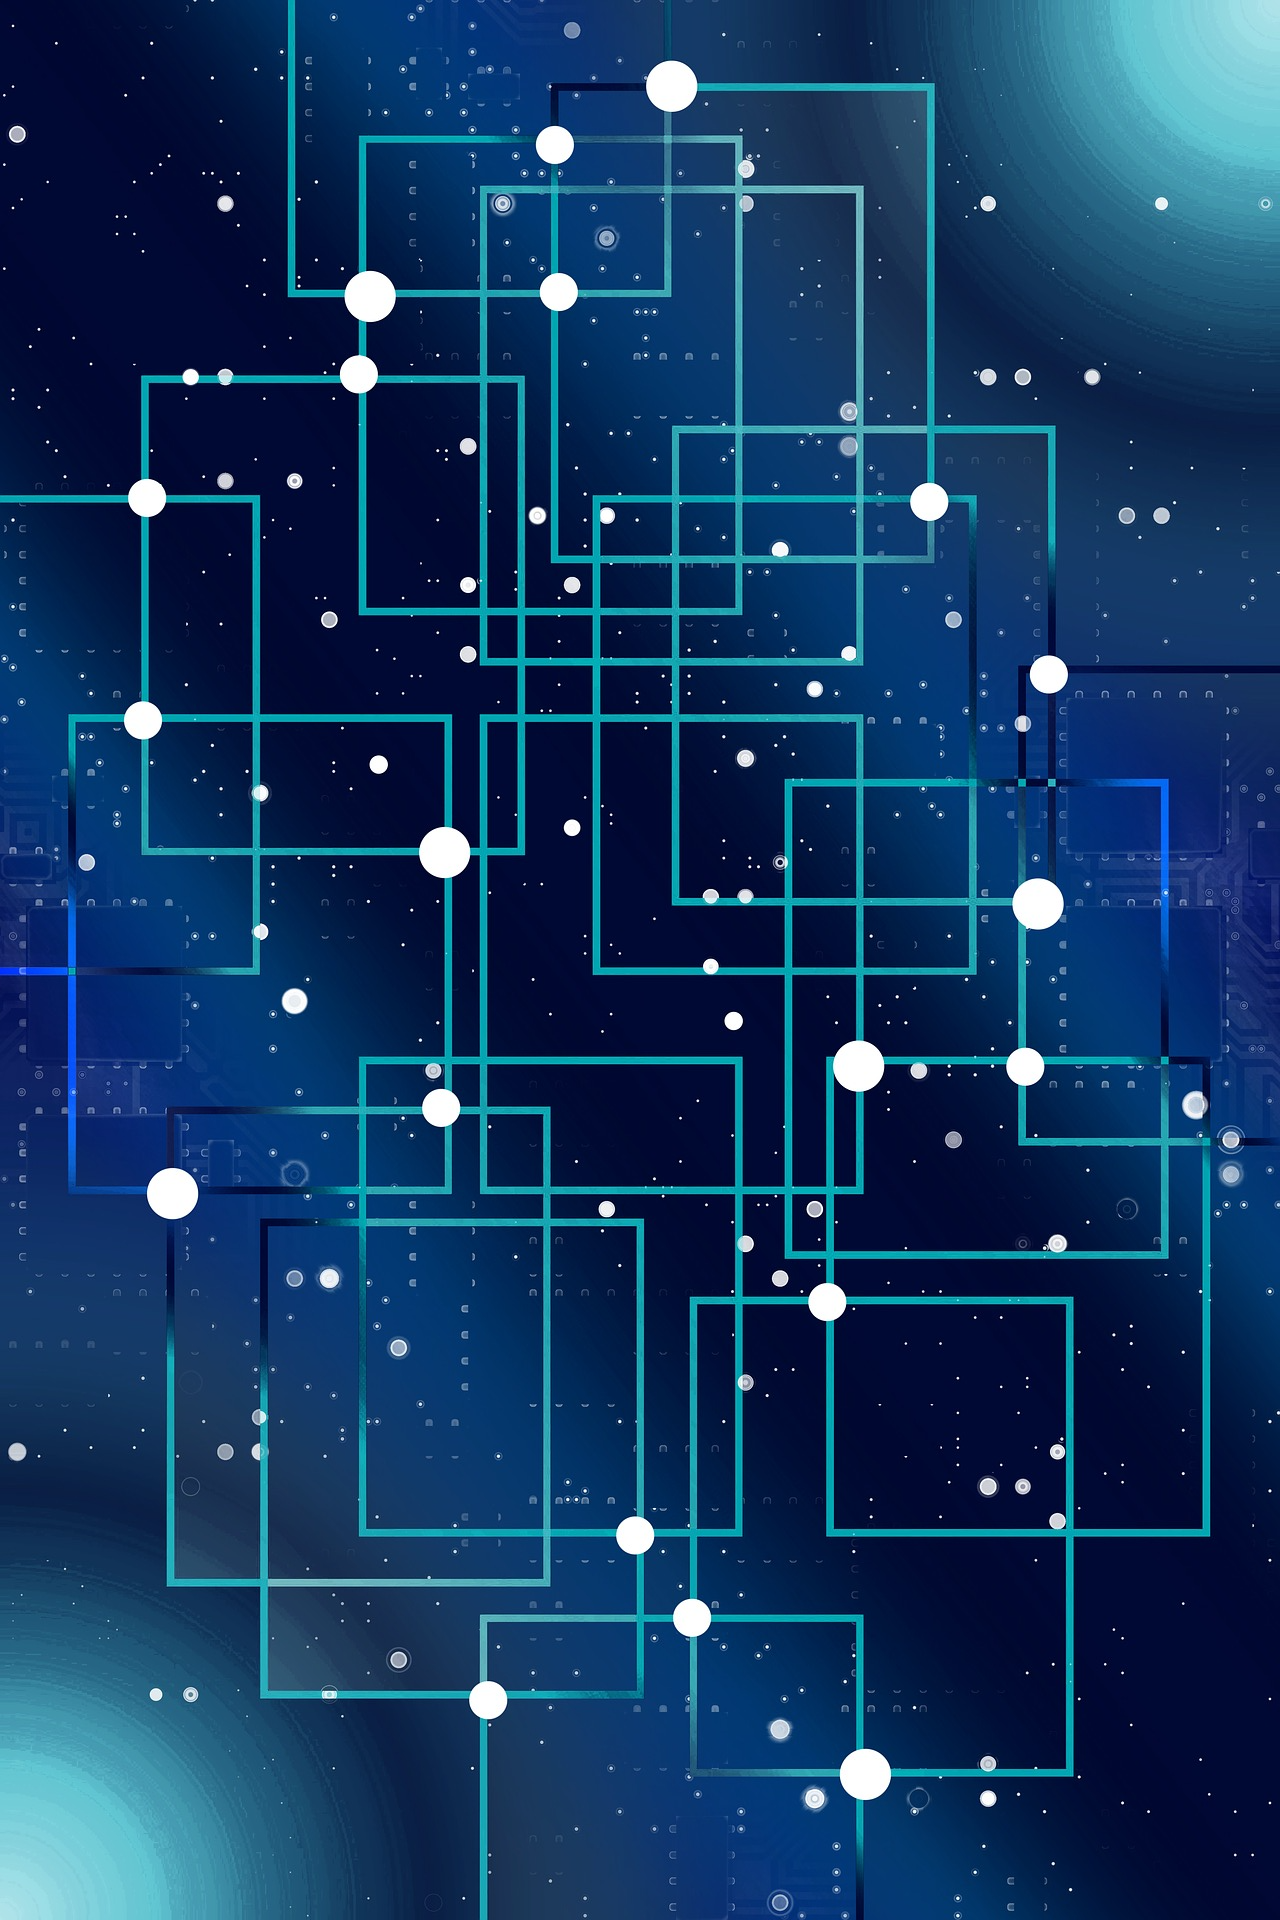
\includegraphics[width=\paperwidth]{background.png}};
\draw (current page.center) node [fill=blue!2!white,fill
opacity=0.9,text opacity=1,inner
sep=1cm]{\Huge\centering\bfseries\sffamily\parbox[c][][t]{\paperwidth}{\centering
    \TITLE \\[15pt] % Book title
{\Large \SUBTITLE}\\[20pt] % Subtitle
{\huge \AUTHOR \\ \Large \EMAIL }}}; % Author name
\end{tikzpicture}
\vfill
\endgroup

%----------------------------------------------------------------------------------------
%	COPYRIGHT PAGE
%----------------------------------------------------------------------------------------

\newpage
~\vfill
\thispagestyle{empty}

\noindent Copyright \copyright\ 2017 \AUTHOR \\

\noindent \EMAIL \\ % Copyright notice

% \noindent \textsc{Indiana University}\\ % Publisher

\noindent \textsc{https://github.com/cloudmesh/classes}\\ % URL

\begin{comment}
\noindent Licensed under the Creative Commons
Attribution-NonCommercial 3.0 Unported License (the ``License''). You
may not use this file except in compliance with the License. You may
obtain a copy of the License at
\url{http://creativecommons.org/licenses/by-nc/3.0}. Unless required
by applicable law or agreed to in writing, software distributed under
the License is distributed on an \textsc{``as is'' basis, without
  warranties or conditions of any kind}, either express or
implied. See the License for the specific language governing
permissions and limitations under the License.\\ % License information

\end{comment}

\noindent \textit{First printing, October 2017} % Printing/edition date

%----------------------------------------------------------------------------------------
%	TABLE OF CONTENTS
%----------------------------------------------------------------------------------------

%\usechapterimagefalse % If you don't want to include a chapter image, use this to toggle images off - it can be enabled later with \usechapterimagetrue

\chapterimage{TOC.png} % Table of contents heading image

\pagestyle{empty} % No headers

\tableofcontents % Print the table of contents itself

\cleardoublepage % Forces the first chapter to start on an odd page so it's on the right

\pagestyle{fancy} % Print headers again



\newcommand{\FILENAME}{\begin{fileremark}\currfiledir
    \currfilename\end{fileremark}}
\newcommand{\CHANGE}{\begin{changeremark}THIS WILL CHANGE
    \currfilename\end{changeremark}}
\newcommand{\TODO}[1]{\todo[inline]{#1}}
\newcommand{\DONE}[1]{DONE: \todo[inline,color=green!30]{#1}}

\newcommand{\FIGURE}[5]{
\begin{figure}[#1] 
  \centering 
    \includegraphics[width=#2\columnwidth]{#3} 
  \caption{#4}\label{#5} 
\end{figure} 
}

\newcommand{\URL}[1]{ \begin{itemize} \item \url{#1} \end{itemize} }
\newcommand{\HREF}[2]{ \begin{itemize} \item \href{#1}{#2} \end{itemize} }

\newcommand{\video}[4]{%
{\em \hfill \href{#4}{#3 (#2)~
\includegraphics[width=\baselineskip]{images/video.png} }}    \index{Video!#1!#3 (#2)}
}

\newcommand{\slides}[4]{%
  {\em  \hfill \href{#4}{#3 (#2)~
\includegraphics[width=\baselineskip]{images/slide.png}}} \index{Slides!#1!#3 (#2)}
}

\DefineVerbatimEnvironment{verbatim}{Verbatim}{xleftmargin=.5in}


\definecolor{codegreen}{rgb}{0,0.6,0}
\definecolor{codegray}{rgb}{0.5,0.5,0.5}
\definecolor{codepurple}{rgb}{0.58,0,0.82}
\definecolor{backcolour}{rgb}{0.97, 0.97, 0.97}
 
\lstdefinestyle{code}{
    backgroundcolor=\color{backcolour},   
    commentstyle=\color{codegreen},
    keywordstyle=\color{magenta},
    numberstyle=\tiny\color{codegray},
    stringstyle=\color{codepurple},
    basicstyle=\footnotesize,
    breakatwhitespace=false,         
    breaklines=true,                 
    captionpos=b,                    
    keepspaces=true,                 
    numbers=left,                    
    numbersep=5pt,                  
    showspaces=false,                
    showstringspaces=false,
    showtabs=false,                  
    tabsize=2
}
 
\lstset{style=code}

\newcommand{\WHERE}[2]{\ref{#1}. \nameref{#1} \hfill ~ #2 ~ \pageref{#1}}

\graphicspath{{./}{images/}{section/cluster/pi/images/}}

\chapter{Big Data Applications and Software}

\FILENAME

\section{Overview}

\slides{i524}{Pages 26}{Overview}{https://drive.google.com/file/d/0Bx_sUfI4VkKSaHlDWkZkeGh4LVE/view?usp=sharing}

\video{i524}{11:29}{Part 1}{https://www.youtube.com/watch?v=Z2M5NsTsj2Y}

\video{i524}{04:10}{Part 2}{https://www.youtube.com/watch?v=5VXhF_Z7Vdk}

\video{i524}{12:41}{Part 3}{https://www.youtube.com/watch?v=DDXqLZcavas}


\section{Introduction}

\slides{i524}{Pages 39}{Course Introduction}{https://drive.google.com/file/d/0Bx_sUfI4VkKSMHBUblVUMWg4Y00/view?usp=sharing}

\video{i524}{0:13:59}{Introduction}{https://www.youtube.com/watch?v=VWK7QdThOPQ}

\video{i524}{0:15:28}{Real World Big Data}{https://www.youtube.com/watch?v=hjrFaXMU1dg&list=PLLO4AVszo1SNIGlqjEBaQjLvc3lgpeI3M&index=2}

\video{i524}{0:10:57}{Basic Trends and Jobs}{https://www.youtube.com/watch?v=u5Y0aKbzync&index=3&list=PLLO4AVszo1SNIGlqjEBaQjLvc3lgpeI3M}

\TODO{on box but not available, move to google drive}

\slides{i524}{Pages ??? }{Acess Patterns, Data Access Patterns and Introduction to using HPC-ABDS}{https://iu.box.com/s/o5rqlsop0jv98lqdon3h9qszk3soq31g}


\video{i524}{0:27:45}{A. Introduction to HPC-ABDS Software and Access Patterns}{https://www.youtube.com/watch?v=6Kj9E38lUzU}


\video{i524}{0:18:38}{B. Science Examples (Data Access Patterns)}{https://www.youtube.com/watch?v=hYJ4_1A4kEU}

\begin{itemize}
\item  Resource 1
  \url{http://grids.ucs.indiana.edu/ptliupages/publications/HPC-ABDSDescribedv2.pdf}
\item Resource 2 \url{http://hpc-abds.org/kaleidoscope/}
\end{itemize}

\video{i524}{11:26}{C. Remaining General Access Patterns}{https://www.youtube.com/watch?v=hsEDKM7Zur4}

\video{i524}{14:32}{D. Summary HPC-ABDS Layers 1 - 6}{https://www.youtube.com/watch?v=zVPKiGV0fk0}

\video{i524}{30:52}{E. Summary HPC-ABDS Layers 7 - 13}{https://youtu.be/6Kj9E38lUzU}

\video{i524}{28:02}{F. Summary HPC-ABDS Layers 14 - 17}{https://www.youtube.com/watch?v=13EQZ-6z91k}

\video{i524}{20:20}{G. Summary HPC-ABDS Others}{https://www.youtube.com/watch?v=0kj-NEl8VF4}

\section{Application Structure}

Big Data Application Structure,Slides \url{https://iu.box.com/s/zl71trvqfw6vv4wnc8xr6gf1qpc9a2dr}

\video{i524}{0:23:25}{NIST Big Data Sub Groups}{https://www.youtube.com/watch?v=12-BlQhnCxc}

\video{i524}{0:23:51}{Big Data Patterns - Sources of Parallelism}{https://www.youtube.com/watch?v=tZfFQw5M8cU}

\video{i524}{0:18:26}{First and Second Set of Features}{https://www.youtube.com/watch?v=PgUGXql34DM}

\video{i524}{0:18:38}{Machine Learning Aspect of Second Feature Set and the Third Set}{https://www.youtube.com/watch?v=mNmmW5ZBjgs}

\section{Application Aspects}

\TODO{slides are on box and not google drive
Aspects of Big Data Applications,Slides \url{https://iu.box.com/s/atgkxucop1lzftkunf8al2fe74x65na6}
}

\video{i524}{0:16:50}{Other sources of use cases and Classical Databases/SQL Solutions}{https://youtu.be/dZRtHaf2MyA}

\video{i524}{0:18:49}{SQL Solutions -  Machine Learning Example -  and MapReduce}{https://www.youtube.com/watch?v=PZDiJNS234A}

\video{i524}{0:20:26}{Clouds vs HPC -  Data Intensive vs. Simulation Problems}{https://www.youtube.com/watch?v=gazESBGLlY8}

\section{Applications}

\TODO{slides are on box and not google drive
Big Data Applications and Generalizing their Structure,Slides \url{https://iu.box.com/s/01dndtucmynekgehur00vktfgcppgc1r}
}

\video{i524}{0:25:20}{NIST UseCases and Image Based Applications Examples I}{https://www.youtube.com/watch?v=tRoAx444A6U}

\video{i524}{0:15:23}{Image Based Applications II}{https://www.youtube.com/watch?v=FDtnWGwotjA}

\video{i524}{0:25:25}{Internet of Things Based Applications}{https://www.youtube.com/watch?v=cOuCSveoVYY}

\video{i524}{0:22:44}{Big Data Patterns - the Ogres and their Facets I}{https://www.youtube.com/watch?v=CvCfRP7J6dU}

\video{i524}{0:15:09}{Facets of the Big Data Ogres II}{https://www.youtube.com/watch?v=fGyUPApnwHw}

\section{Other}

\video{i524}{0:24:00}{More of Software Stack}{https://www.youtube.com/watch?v=apDXH_eVnEc}




\begin{comment}

\chapter{Course Policies}\label{C:course-2018}

\FILENAME

\begin{WARNING}
  As the class material will evolve during the semester it is obvious
  that some content will be improved and material will be added. This
  benefits all classes. To stay up to date, please, revisit this
  document on weekly basis. This is obvious, as we will adapt content
  based on your feedback. 

  The requirement of the classes to become an expert in cloud and/or
  Big Data applications and technologies stays unchanged.
\end{WARNING}


Residential students are required to attend all Friday classes
including those held in May.  Missing such classes will result in
grade reduction. Based on past class experience we are foced to
implement a strict strict policy. Only for medical reasons a class can
be missed. The reasoning for this is that residential students that
did not attend classes regularly tend to do not as well in this class
as their colleagues. As we want that you achieve your best we strongly
advise to attend and give with this policy an additional motivating
factor.

\section{HID}

You will be assigned an hid (Homework IDentifier) which allows us to
easily communicate with you and doe allow us to not use your
university ID to communicate with you. 

You will receive the HID within the first week of the semester by the
TA's.

\section{Notebook}\label{notebook}

All students are required to maintain a \emph{class notebook} in
github in which they summarize their weekly activities for this course
in bullet form. This includes a self maintained list of which lecture
material they viewed.

The notebook is maintained in the class github.com in your hid project
folder. It is a file called notebook.md that uses markdown as format.
While using md, you can either edit it locally and upload to github, or
directly edit it via the git hub Web editor.

You will be responsible to set up and maintaining the notebook.md and
update it accordingly. We suggest that you prepare sections such as:
Logistic, Theory, Practice, Writing and put in bullet form what you have
done into these sections during the week. We can see from the github
logs when you changed the notbook.md file to monitor progress. The
management of the notebook will be part of your discussion grade.

The format of the notebook is very specific markdown format and must
follow these rules:

\begin{itemize}
\item use headings with the \# character and have a space after the \#
\item use bullets in each topic.
\item each bullet \textbf{must} have an individual date that is of the
  form mm/dd/yy. Please do not lump bullet points under s single
  date. Have each bullet point its own date
\item if you have done the activity in a period than add the second
  date to it mm/dd/yy - mm/dd/yy
\item If you refer to section numbers in your notebook, please aslo
  add the section title as the section numbers may change in case we
  need to add content
\end{itemize}

Please examine carefully the sample note book is available at:

  \URL{https://raw.githubusercontent.com/bigdata-i523/sample-hid000/master/notebook.md}

This will render in git as:

  \URL{https://github.com/bigdata-i523/sample-hid000/blob/master/notebook.md}

The notebook.md is not a blog and should only contain a summary of
what you have done. 

\section{Blog}

Optional: If you like to maintain your own blog, you can create yourself also a
blog.md file. However do not include sensitive information in
there. A blog is not a replacement for the notebook.

\section{Calendar I524, E616, E516}\label{S:calendar}

This class is a full term class of 16 weeks.

\begin{IU}

The semester calendar is posted at 

\URL{http://registrar.indiana.edu/official-calendar/official-calendar-spring.shtml}

The class beginns Mon, Jan 8th and ends Fri, May 4th

\end{IU}

\begin{longtable}{p{3cm}p{11cm}}
  \caption{Calendar} \\   
  \toprule
  Date & Activity \\
  \midrule
  \endfirsthead
  \toprule
  Date & Activity \\
  \endhead
  \hline
  \multicolumn{2}{c}{Continued}\\   \bottomrule
  \endfoot
  \bottomrule
  \endlastfoot

  Jan 8, Mon & Class Begins\\
  
  Jan 15, Mon 9am & Setup communication pathways for the class. (1)
  You must have created a github repository in our class repository.
  (2) You must be in the class Piazza.  (3) Motivation: if we can not
  communicate with you we can not conduct the class. Everyone must be
  in piazza and github timely.  \\

  Weekly & contribution to notebook.md \\
  Weekly & contribution to piazza and/or the Handbook \\

  Jan 15, Mon & MLK Jr. Day. Good day to work on projects, computer setup \\
  Jan 22, Mon 9am & Tutorial 1 \\
  Feb 5,  Mon 9am & Tutorial 2 \\
  Feb 26, Mon 9am & Paper 1 \\
  Mar 5, Mon 9am & Project draft paper due without panelty \\
  \hline
  Spring Break &\\
  Mar 11 - Mar 18.  & This is a good time to work ahead or catch up
  with things. We strongly advise to use this time wisely. \\
  \hline
  Mar 16, Mon 9am & Project reports due without penalty \\
  Mar 23, Mon 9am & Improvments to Projects and documents possible,
  but substential work must have been done before to not encounter a
  grade reduction \\
  May 1 & Any paper submitted after May 1st will get an
  incomplete and a grade reduction. \\
\end{longtable}

\section{Incomplete}\label{incomplete}

Incompletes have to be explicitly requested in piazza. All incompletes
have to be filed by May 1st.

Incomplete's will receive a fractional Grade reduction: A will
become A-, A- will become B+, and so forth. There is enough time in the
course to complete all assignments without getting an incomplete.

Why do we have such a policy? As we teach state-of-the-art software this
software is subject to change, not only within the course, but also
after the course. As we may offer some services and only have access to
the TA's during the semester it is obvious that we like all class
projects and homework assignments to be completed within a semester.
Services that were offered during the semester may no longer be
available after the semester is over and could adversely effect your
planing. It will be in the students responsibility to identify such
services and provide alternatives if they become unavailable. We try
hard to avoid this but we can not guarantee it.

Furthermore, once an incomplete is requested, you will have 10 month to
complete it. We will need 2 month to grade. No grading will be conducted
over breaks. This may effect those that require student loans. Please
plan ahead.

The incomplete request needs to be off the following format in piazza:

\begin{verbatim}
Subject: 
    INCOMPLETE REQUEST: HID000: Lastname, Firstname

Body:
    Firstname: TBD
    Lastname: TBD
    HID: TBD
    Semester: TBD
    Course: TBD
    Online: yes/no

    URL notebook: TBD    
    URL tutorial1: TBD
    URL tutorial2: TBD
    URL paper1: TBD
    URL project: TBD

    URL other1: TBD
\end{verbatim}

Please make sure that the links ar e clickable in piazza.

\section{Registration Information}\label{registration-information}

The folloing course numbers are sections of this class

The official registration information can be found here:

\begin{itemize}
\tightlist
\item
  \url{http://registrar.indiana.edu/official-calendar/official-calendar-fall.shtml}
\end{itemize}

We summarize, but like to point out that the information here may have
changed. We advise to visit the official page. However important to note
is that all residential students meet:

\begin{verbatim}
09:30A-10:45A   Friday      I2 150 
\end{verbatim}

\subsection{E516}

\begin{verbatim}
ENGR-E 516  ENGINEERING CLOUD COMPUTING (3 CR)
              ***** RSTR     ARR             ARR    ARR       Von Laszewski G
                 Above class taught online
                 Above class open to graduates only
                 Discussion (DIS)
              33699 RSTR     11:15A-12:30P   F      I2 150    Von Laszewski G
\end{verbatim}

\begin{verbatim}
        ENGR-E 516  ENGINEERING CLOUD COMPUTING (3 CR)
              33909 RSTR     ARR             ARR    WB WEB    Von Laszewski G
                 This is a 100% online class taught by IU Bloomington. No
                 on-campus class meetings are required. A distance education
                 fee may apply; check your campus bursar website for more
                 information
                 Above class open to graduates only
\end{verbatim}

\subsection{I524 and E616}

These classes are identical. In this courses we will be focussing on
Advanced Cloud COmputing and Big Data Applications and Analytics.  It
covers the applications and technologies needed to process the
application data. It uses Clouds running Data Analytics
Collaboratively processing Big Data to solve real problems.

Intelligent Systems Engeneering:

\begin{verbatim}
	ENGR-E 616  ADVANCED CLOUD COMPUTING (3 CR)
              ***** RSTR     ARR             ARR    ARR       Von Laszewski G
                 Above class taught online
                 Above class open to graduates only
                 Discussion (DIS)
              33697 RSTR     09:30A-10:45A   F      I2 150    Von Laszewski G
\end{verbatim}

Info Residential:



\begin{verbatim}
INFO-I 524  BIG DATA SOFTWARE AND PROJECTS (3 CR) 
              ***** RSTR     ARR             ARR    ARR       Von Laszewski G          
                 Above class open to graduates only
                 Above class taught online
                 Discussion (DIS)
              13053 RSTR     09:30A-10:45A   M      I2 130    Von Laszewski G  
\end{verbatim}

\begin{WARNING}
The location and time of this class is going to change to Friday
09:30A-10:45A   room I2 150.  
\end{WARNING}

Info Online:

\begin{verbatim}        
        INFO-I 524  BIG DATA SOFTWARE AND PROJECTS (3 CR)
              13054 RSTR     ARR             ARR    ARR       Von Laszewski G          
                 Above class open to graduates only
                 This is a 100% online class taught by IU Bloomington. No
                 on-campus class meetings are required. A distance education
                 fee may apply; check your campus bursar website for more
                 information
\end{verbatim}

\subsection{E222}

Undergraduate:

In this course students will be familiarized with different specific 
applications and implementations of intelligent systems and their use 
in desktop and cloud solutions.

\begin{verbatim}
ENGR-E 222  INTELLIGENT SYSTEMS II (3 CR)
              ***** RSTR     02:30P-03:45P   TR     GY 436  Fox
                 Laboratory (LAB)
        E 222 : P - ENGR-E 221
              31434 RSTR     05:45P-06:35P   R      GY 447  Fox
                 Above class for  Intelligent Systems Engineering students

\end{verbatim}        



\section{Waitlist}\label{waitlist}

The waitlist contains students that are unable to enroll in a section of
a course. Students choose to add themselves to the waitlist. They are
not automatically added, but choose to do so intentionally based on the
status of the course. There are two reasons for students to be on the
waitlist. The first, and primary, reason is that the class is already at
the scheduled, maximum capacity. Since there are no seats available, the
student can elect to add themselves to the waitlist. The second reason
is that the students' own schedule has a time conflict. This occurs when
they are trying to enroll in a class that overlaps with the time of a
class they are already enrolled in.

Students are moved from the waitlist to the regular section during a
daily batch process, and not in real time. The process is not in
realtime because the registrar receives many requests to increase
capacity, decrease capacity, and change rooms. If the process were real
time there would be a catastrophe of conflicts.

Students are moved from the waitlist in chronological order that they
added themselves to the waitlist. If you are still on the waitlist there
are no spaces free, the batch process has not run for the day, or the
student in question has a schedule conflict.

Faculty are not able to selectively choose students from the waitlist.

How long does the waitlist process stay active?: The automated
processing of the waitlist ends on Thursday of the first week of class
At this time the waitlist will no longer be processed. 
As the residential class starts on Friday, this may cause
issues. Either talk to the department on Thursday or show up on
Friday. Most likeley there will be spaces left. 
Students on the waitlist at that time will remain on the waitlist, but remain there
until the student decides to change their registration. Students may not
do that, because they get assessed a change schedule fee.

Students tell me they still want to enroll after the first week of
classes. How do they do this?

Beginning Monday, after the first week of class students begin to use
the eAdd process to do a late addition of the course. The request is
routed to the professor of record on an eDoc and the faculty will be
notified via email. Faculty can deny or approve based on whatever
criteria they wish to apply. If the faculty member approves, the eDoc
is electronically forwarded to the Academic Operations office and we
will approve the late add \textbf{if the room capacity} allows the
addition, otherwise we must deny the addition because of fire marshal
regulations. Many times, there are seats in a
classroom/discussion/lab, but because other students have not
\emph{officially} dropped, enrollment is still at capacity.

After everything, a student that was unable to enroll in the class
attended all year and completed all course work as if they had enrolled.
Can the student get credit and can I give the student a grade?

Yes. There is a provision for a late registration - contact our office
if this occurs. Students will be assessed a tuition fee at the time of
late or retroactive registration.

\section{Auditing the class}\label{auditing-the-class}

We no longer allow students to audit I524, E516, and E616. The
motivation to not offer these classes for auditing are:

\begin{itemize}
\item Seating in the lecture room is limited and we want foster
  students that enroll full time first.

\item The best way to take the class is to conduct a project. As this can
not be achieved without taking the class full time and as auditing the
class does not provide the full value of the class, e.g. not more than
10\% of the class, we do not think it is useful to audit the class.

\item  Accounts and services have to be set up and require
  considerable resources that are not accessible to students that
  audit the class.

\end{itemize}


\section{Resource restrictions}

\begin{itemize}
\item It is not allowed to use our services for profit (e.g. just
  enrolling in the class to use our clouds).
\item In case of abuse of available compute time on our clouds the
  student is aware that we will terminate the computer account on our
  clouds and she may have to conduct the project on a public cloud or
  his own computer under her own cost. There will be no guarantee that
  cloud services we offer will be available after the semester is
  over.  Projects can be conducted as part of the class that do not
  require access to the cloud.
\end{itemize}

\section{Meeting Times}\label{meeting-times}

The classes are published online. Residential students at Indiana
University will participate in a discussion taking place at the
following time according to the information provided by the registrar.

\begin{itemize}
\item 09:30A-10:45A Friday I524/E616 residential, I2 150
\item  11:15A-12:30A Friday I516 residential, I2 150
\end{itemize}

The Monday class is moveing to Friday, if this is introducing a
conflict, let us know.

\section{Office Hours}\label{office-hours}

\begin{description}

\item[Online Students:] Online hours are prioritized for online students,
  residential students should attend the residential meetings. 

\item[Residential Students:] Residential students participate in the
  official meeting times. If additional times are required, they have
  to be done by appointment. Office hours will be announced
  publically. All technical office hours are public and can be
  attended by any student.

  Online houres are not an excusenot to come to the residential class.

  However Residential students can in addition to the residential
  class use the online student meeting times.  However, in that case
  online students will be served first. It is probably good to check
  into the zoom meeting and identify if the TA has time. They will be
  in zoom.

\end{description}

We suggest that you let the TA's know in piazza before you come, in order to make
sure they are at the office.

\begin{itemize}
\item Mon 6:00pm-7:00pm, 7:00pm-8:00pm, Gregor (online)
\item Tue TBD, Smith Research Center
\item Wed TBD, Smith Research Center
\item Thu TBD, Smith Research Center
\item Fri TBD, Smith Research Center
\item Sat TBD, Smith Research Center
\end{itemize}


If a meeting is needed with Gregor, this is done upon appointment
Tue-Thu 10am - 2:30pm. However, TA's will figure out if a meeting is needed.
Please prepare your technical questions ahead of time, and place them in Piazza
first. TA's and the class will try to answer them if possible

The link for joining the meeting on Zoom is posted in Piazza.

% \URL{https://iu.zoom.us/j/235405252}

\URL{TBD}

For more up-to-date details, refer to Piazza.

\section{Plagiarizm}

On teh first day of class you will need to read the information about
plagiarizm. If there are any questions about plagiarizm we require you
to take a course offered from the IU educational department.

\begin{WARNING}
  If we find cheating or plagirizm, your assignment will be receiving
  an {\em F}. This especially includes copying text without proper
  attribution. In addition you will be receiving an {\em F} for the
  appropriate time for the discussion points an assignment was issued,
  e.g. If a paper duration assignment is 4 weeks, you get for these
  four weeks no discussion points, meaning an {\em F}. Furthermore, we
  will follow IU policy and report your case to the dean of students
  who may elect to expell you form the university. Please understand
  that it is your doing and the instructors have no choice as to
  follow university policies. Do not blame the instructors. Excuses
  such as ``I missed the lecture on plagiarizm'', ``I forgit to
  include the original refrence as I ran out of time'', ``I did not
  understand what plagiarizm is'' do not count obvioulsy as we
  explicitly make the policies clear. This applies to all material
  prepared for class including assignments, excercises, code,
  tutorials, papers, and projects
\end{WARNING}

For more information on this topic please see:

\URL{https://studentaffairs.indiana.edu/student-conduct/misconduct-charges/academic-misconduct.shtml}
\FILENAME

\section{About the Course}\label{about-the-course}

The Big Data Applications and Analytics course is an overview course in
Data Science and covers the applications and technologies (data
analytics and clouds) needed to process the application data. It is
organized around rallying cry: Use Clouds running Data Analytics
Collaboratively processing Big Data to solve problems in X-Informatics.


\section{Tutorials, Topic Paper, Term Paper, Project Report}

\FILENAME

Dependendt on the class you need to do different assignments. The
assignments will be clearly posted in this document and updated in
case clarification is needed. 

We use the following terminology:

\begin{description}

\item[Tutorials:] Tutorials are written in markdown, RST, or LaTeX and
  include information on a particular technical issue that is in
  general helpful for other students. Tutorials can be small, but sume
  may need to be substential. As we expect that the tutorials can be
  included in the Handbook, please be careful of plagiarizm and do not
  just copy the tutorial from elswhere. 

\item[Topic Paper:] A topic paper, or short paper is a smapp paper
  about a technology, application, or useful information that provides
  an overview of what you are trying to describe and analyses its
  relatinship to the class topic. Be mindful about plagiarizm. The
  paper is written in \LaTeX and uses jabref for bibliography management. 

\item[Term Paper:] A term paper is an enhanced topic paper. The
  difference is in length. Comparative or review papers can also be
  term papers.  Term papers should have the quality to be publishable
  either in a workshop or as part of the handbook.

\item[Project Paper:] A project reportis an enhanced topic paper that
  includes not just the analysis of a topic, but an actuall code, with
  benchmark or demosntarted appliction use. Obviously it is longer
  than a paper and includes descriptions about reproducability of the
  application. Term papers should have the quality to be publishable
  either in a workshop or as part of the handbook.

\item[Assignments:] In addition to the previously discussed toppict
  you also are doing a small number of assignments. These assignments
  may take you one or multiple weeks to accomplish. Some of them are
  pass fail, while others will receive a grade. It will be clearly
  stated at the beginning of the assignment which of the evaluation
  will apply.

\end{description}

Examples from prior classes are avalable in the class proceedings
listed in Section~\ref{S:p-intro}.

Dependent on the class you have to fulfill different
requirements. Please make sure you understand which requirement you
will have.

\begin{description}

\item[E516] In these classes you will need to produce
  tutorials, topic papers and a project report with real code.

\item[E616] In these classes you will need to produce
  tutorials, topic papers and a project report with real code. 

\item[I524] same as E616, but you have the choice to
  substitute the project report with a term paper.

\end{description}

Please be aware that the project or term paper constitute to a
significant portion of your grade of your class grade. You have plenty
of time to make this choice and if you find you struggle with
programming you may want to consider a term paper instead of a
project.

In case you chose a project your maximum grade for the entire class
could be an A+. However, an A+ project must be truly outstanding and
include an exceptional project report. Such a project and report will
have the potential quality of being able to be published in a
conference.

In case you chose a term Paper for I524 your maximum grade for the
\textit{entire} class will be an A-.

Please note that a project includes writing a project paper.  However
the length is a bit shorter than for a term paper.

\subsection{Team}

Software projects and term papers can be conducted with one, two or
three class members. We do not allow more than three members in a
project, paper, or assignment team. It will be up to you to determine
a team, but we recommend that you chose wisely. Naturally if a team
member does not contribute to the project you need to address this
early on. Please do not come to us a week before the deadline is due
and say a team member has not contributed, this is far to late to do
any adjustment to the team. It is in your responsibility to manage the
team. You can build different teams throughout the semestar for
different tasks. Please communicate clearly and timely with your
class mates.

\subsection{Common Deleiverables}

Both Projects and Term paper have the following common deliverables

\begin{description}
\item[Work Breakdown:]
This is an appendix to the document that describes in detail who did
what in the project. This section comes in a new page after the
references. It does not count towards the page length of the document.
It also includes explicit URLs to the the git history that documents the
statistics to demonstrate not only one student has worked on the
project. If you can not provide such a statistic or all checkins have
been made by a single student, the project has shown that they have not
properly used git. Thus points will be deducted from the project.
Furthermore, if we detect that a student has not contributed to a
project we may invite the student to give a detailed presentation of the
project.
\item[Bibliography:]
All bibliography has to be provided in a jabref/bibtex file. This is
regardless if you use LaTeX or Word. There is \textbf{NO EXCEPTION} to
this rule. PLease be advised doing references right takes some time so
you want to do this early. Please note that exports of Endnote or other
bibliography management tools do not lead to properly formatted bibtex
files, despite they claiming to do so. You will have to clean them up
and we recommend to do it the other way around. Manage your bibliography
with jabref, and if you like to use it import them to endnote or other
tools. Naturally you may have to do some cleanup to. If you use LaTeX
and jabref, you have naturally much less work to do. What you chose is
up to you.
\item[Report Format:]
All reports will be using the our common format. This format is not the
same as the ACM format, so if you use systems such as overleaf or
sharelatex, you need to upload it and use it there.

The format for LaTeX and Word found here:

  \URL{https://github.com/bigdata-i523/sample-hid000/tree/master/paper1}

\end{description}

There will be \textbf{NO EXCEPTION} to this format. In case you are in a
team, you can use either github while collaboratively developing the
LaTeX document or use MicrosoftOne Drive which allows collaborative
editing features. All bibliographical entries must be put into a
bibliography manager such as jabref, endnote, or Mendeley. This will
guarantee that you follow proper citation styles. You can use either ACM
or IEEE reference styles. Your final submission will include the
bibliography file as a separate document.

Documents that do not follow the ACM format and are not accompanied by
references managed with jabref or endnote or are not spell checked will
be returned without review.

\TODO{Integrate the format from the class web page into the LateX
  section More details about the format can be found at
  \url{https://cloudmesh.github.io/classes/lesson/doc/report.html} }

\subsection{Project Paper}

\subsubsection{Systems Usage}

Projects may be executed on your local computer, a cloud or other
resources you may have access to. This may include:

\begin{itemize}
\item chameleoncloud.org
\item furturesystems.org
\item AWS (you will be responsible for charges)
\item Azure (you will be responsible for charges)
\item virtualbox if you have a powerful computer and like to prototype
\item other clouds, please confirm with us.
\end{itemize}

Access to clouds must be scripted and a cmd5 extension must be
developed as part of your project to receive full credit.

\subsubsection{Deliverables}

The following artifacts are part of the deliverables for a project

\begin{description}
\item[Code:]
You must deliver the \textbf{source code} in github. The code must be
compilable and a TA may try to replicate to run your code. You MUST
avoid lengthy install descriptions and everything must be installable
from the command line. We will check submission. All team members must
be responsible for one or all parts of the project.

Code repositories are for code, if you have additional libraries that
are needed you need to develop a script or use a DevOps framework to
install such software. Thus zip files and .class, .o files are not
permissible in the project. Each project must be reproducible with a
simple script. An example is:

\begin{verbatim}
git clone ....
make install
make run
make view
\end{verbatim}

Which would use a simple make file to install, run, and view the
results.  You are expected to integrate cmd5, which we teach in
class. In addition you can use or are expected to us DOCKERFILES,
ansible, or shell scripts. It is not permissible to use GUI based
DevOps preinstalled frameworks. Everything must be installable and
reproducable form the command line.

\item[Data:] Data is to be hosted on IUs google drive if needed. If
  you have larger data, it should be downloaded from the internet. It
  is in your responsibility to develop a download program,
\item[Project Report:] A report must be produced while using the
  format discussed in the Report Format section. The following length
  is required:

\begin{itemize}
\item
  6 pages, one student in the project
\item
  8 pages, two students in the project
\item
  10 pages, three students in the project
\end{itemize}

\item[License:] All projects are developed under an open source
  license such as Apache 2.0 License. You will be required to add a
  LICENCE.txt file and if you use other software identify how it can
  be reused in your project. If your project uses different licenses,
  please add in a README.rst file which packages are used and which
  license these packages have.
\end{description}

\subsection{Term Paper}

In case you chose the term paper, you or your team will pick a topic
relevant for the class. You will write a high quality scholarly paper
about this topic. The following artifacts are part of the deliverables
for a term paper. A report must be produced while using the format
discussed in the Report Format section. The following length is
required:

\begin{itemize}
\item 8 pages, one student in the project
\item 10 pages, two student in the project
\item 12 pages, three student in the project
\end{itemize}


\section{Grading}\label{grading}

Grading for homework will be done within reasonable time of the
submission if the submission was on time. This however could still
take multiple weeks. Students that miss the deadline will be graded on
best effort, which could mean at the end of the semester as TAs will
grade first papers that have been handed in on time.  A 10\% grade
reduction will be given for residential students if the project is
late.  Some homework can not be delivered late (which will be clearly
marked and 0 points will be given if late; these are mostly related to
setting up your account and communicating to us your account names.)

It is the student's responsibility to upload submissions well ahead of
the deadline to avoid last minute problems with network connectivity,
browser crashes, cloud issues, etc. It is a very good idea to make early
submissions and then upload updates as the deadline approaches; we will
grade the last submission received before the deadline.

Note that the term paper or project paper will take a considerable
amount of time and doing proper time management is a must for this
class. Avoid starting your project late. Procrastination does not pay
off. Starting a paper a day or even in the week before the deadline
will allow you not to achieve your best. Late Projects or term papers
will receive a 10\% grade reduction.

For E516 I524, E616 the grading scene is discussed in the syllabus.


\subsection{Grades on Canvas}

The final grade for your class is {\bf NOT} accurately posted in
CANVAS. Please visit the registrar for your final grade.
We have run many times into issues with CANVAS thus we try to stay as
much as possible away form it. We know that the total grade will not
be accurately reported in CANVAS.

Furthermore we are using only a letter grading scheme that
distinguishes qualitatively between grades. Typically we do not engage
in arguing if you get a point more or less. Instead we look at the
artifact and decide if it is an A or A- and so on. CANVAS on the other
hand uses a point system that may provide a misleading information as
we do not use points.

Once the due date is passed all incomplete assignments will appear as
an \textit{F} in CANVAS. Once we receive and review the submission this grade will
be changed. Please, do not cintact us if you submitted late and you
see an F in CANVAS temportrarily.

\subsection{Discussion about Grades}

Should it be necessary a discussion about a grade must not be taking
place via e-mail nor via piazza. YOu must use the CANVAS message
feature as we want to make sure that by accident you post information
to others that you do not intend to. FOr this reason we will not read
such messages on pizza and in our e-mail and deleted them without reading.

\part{Assignments}

\section{Overview}
\FILENAME

We will post in this part all assignments for the various classes. As
this page will be updated frequently, it is in the students
responsibility to check.

It is in the
responsibility of the student to check this page and complete the
assignments. Some assignment may not be graded, but they still have to
be completed. To identify the assignment they carry the name of the
Lesson as well as a number. We try to alsoinclude a refernce to the
section where this assignment may be originating from.

The following are mandated assignments for this class

\section{Due Dates}

If not explicitly mentioned here the due dates are posted in Section
\ref{S:calendar}.

\section{Deliverables}

You will have graded assignments as documented in Section
{C:course-2018}. In addition we will post here some additional
assignments, some of which are pass/fail and are integrated in your
disccussion points. You will need to add them to your notebook and if
code is required to include an explicit URL to where that particular
code is in your git repository.

\section{Week 1}

Using Piazza

\begin{itemize}
\item  Watch the introduction video at:
  \url{https://youtu.be/yC3PNkb_9mI}
\item Exercise.Piazza.1 e-piazza
\item Exercise.Piazza.2 e-piazza
\item Exercise.Piazza.3 e-piazza
\item Exercise.Organization.1 e-organization
\item Exercise.Organization.2 e-organization
\item Exercise.Organization.3 e-organization
\item Exercise.Organization.4 e-organization
\item Exercise.Organization.5 e-organization
\item 
  Conduct the entry survey after you have done the above assignments:
  \TODO{Old link:
  \url{https://piazza.com/class/j5wll7vzylg25j?cid=67}, new links will
be different for class}

\item 
  Learn about Piazza folders:
  \TODO{old link:
  \url{https://piazza.com/class/j5wll7vzylg25j?cid=103}, new links
  will be different for class}
\end{itemize}

Optional Assignment:

\begin{itemize}
\item Buy Hardware for IoT
\TODO{e616 will have hardware
  \url{https://piazza.com/class/j5wll7vzylg25j?cid=55}}
\end{itemize}

Complete the above within the first week!

\begin{comment}
\section{Week 2}\label{week-2}

This may take multiple weeks to complete for some of you:

Learn on how to use piazza for the class

\begin{itemize}
\item Exercise.Piazza.4 e-piazza
\end{itemize}

Learn Python

\begin{itemize}
\item Exercise.Python.1 e-python
\end{itemize}

\begin{description}
\item[Paper 1 Topic:]
Identify the topic for your individual paper 1 and post it on Piazza:
\url{https://piazza.com/class/j5wll7vzylg25j?cid=158} . The paper will
be due on Oct 9, 9am.
\end{description}

\section{Week 3}\label{week-3}

This assignment may take some of you multiple weeks.

Implement a command using

\begin{itemize}
\tightlist
\item
 Exercise.CMD5.2 e-cmd5
\end{itemize}

that is called ``hello'' that prints hello world. Use docopts to define
the command.

Use cms sys generate command hello

There will be a tutorial about this.

Learning about Git pull Requests while using the Class web page as
example. Only make small changes based on a paragraph and create a pull
request for it.

\begin{itemize}
\tightlist
\item
 Exercise.Contrib.0 e-contrib
\item
 Exercise.Contrib.1 e-contrib
\item
 Exercise.Contrib.5 e-contrib
\end{itemize}

There will be tutorials about this

\begin{description}
\item[Polls]
Please fill out the following polls on Piazza. They will used to track
your progress:

\begin{itemize}
\tightlist
\item
  Who has or will have a Raspberry Pi or esp8266?
  \url{https://piazza.com/class/j5wll7vzylg25j?cid=182}
\item
  Where do you intend to program in python?
  \url{https://piazza.com/class/j5wll7vzylg25j?cid=183}
\item
  What is your python knowledge?
  \url{https://piazza.com/class/j5wll7vzylg25j?cid=184}
\item
  Which lectures did you view?
  \url{https://piazza.com/class/j5wll7vzylg25j?cid=185}
\end{itemize}
\end{description}

\section{Week 4}\label{week-4}

Please identify your paper 2 topic immediately. Post it in the Followup
Discussion section of this Piazza post with the specified format:
\url{https://piazza.com/class/j5wll7vzylg25j?cid=187}

\section{Week 5}\label{week-5}

\begin{itemize}
\item
  Please read the following post on Piazza and make sure your README.md
  file is up to date (Deadline: Friday 22 Sept 9am):
  \url{https://piazza.com/class/j5wll7vzylg25j?cid=252}
\item
  \begin{description}
  \item[Experiments]
  A number of experiments are posted on Piazza. They are not
  assignments, but are experiments and if you do them right, they will
  lead to material that can be shared with all students. Experiments can
  lead to discussion points that go into your discussion grade. Here are
  the links:

  \begin{itemize}
  \tightlist
  \item
    Description \url{https://piazza.com/class/j5wll7vzylg25j?cid=240}
  \item
   Exercise.: Experimenting with gitbash on windows
    \url{https://piazza.com/class/j5wll7vzylg25j?cid=236}
  \item
   Exercise.: Experimenting Windows Subsystem for Linux Documentation
    \url{https://piazza.com/class/j5wll7vzylg25j?cid=237}
  \item
   Exercise.: Experimenting with MQTT
    \url{https://piazza.com/class/j5wll7vzylg25j?cid=238}
  \item
   Exercise.: Experimenting with Graphs
    \url{https://piazza.com/class/j5wll7vzylg25j?cid=239}
  \item
   Exercise.: Experimenting with IoT sculptures
    \url{https://piazza.com/class/j5wll7vzylg25j?cid=241}
  \item
   Exercise.: Build a camera enhanced Raspberry Pi robot car
    \url{https://piazza.com/class/j5wll7vzylg25j?cid=242}
  \item
    Exercise: Build a Raspberry PI docker swarm cluster
    \url{https://piazza.com/class/j5wll7vzylg25j?cid=243}
  \end{itemize}
  \end{description}
\end{itemize}

\section{Week 6}\label{week-6}

Group activity for Residential Students

Work on one of the following discussion posts on Piazza. You will work
in groups that were formed in the class on Friday Sep 25. Post the
results of your work on Piazza by next Thursday (Oct 5) 11:59 PM

\begin{itemize}
\tightlist
\item
  Python 2 vs 3 \url{https://piazza.com/class/j5wll7vzylg25j?cid=333}
\item
  Data formats \url{https://piazza.com/class/j5wll7vzylg25j?cid=334}
\item
  Cloudmesh.cmd5 \url{https://piazza.com/class/j5wll7vzylg25j?cid=335}
\item
  Raspberry Pi \url{https://piazza.com/class/j5wll7vzylg25j?cid=336}
\item
  open: cloudmesh.cmd5 on Windows Native and with docker
  \url{https://piazza.com/class/j5wll7vzylg25j?cid=337}
\item
  open: MQTT \url{https://piazza.com/class/j5wll7vzylg25j?cid=338}
    
\end{itemize}

\end{comment}

\FILENAME

\section{Piazza}\label{piazza}

We use Piazza (\url{https://piazza.com}) because questions and answers
on Piazza are community-edited. Each question has a single answer edited
by the students of the class and if needed an instructors' answer that
is collaboratively edited by the instructors.

Due to this wiki-style Q\&A, when a student has a question, one does not
have to look through long e-mail threads but instead can look at the
answer. For details that lead up to the answer you are highly encouraged
to also look at some comments that lead up to the answer

An advertisement video from Piazza summarizes the features:

\begin{itemize}
\tightlist
\item
  \url{https://www.youtube.com/watch?v=2jLSiN8E18w}
\end{itemize}

Piazza Support with a lot of information is available at:

\begin{itemize}
\tightlist
\item
  \url{http://support.piazza.com}
\end{itemize}

\subsection{Access to Piazza from
Canvas}\label{access-to-piazza-from-canvas}

Piazza is one of the recommended IU supported technologies within
Canvas. It replaces the CANVAS discussion groups with superior
technology targeted to support large student classes while also
focussing on student engagement.

To access piazza you can have the following situations provided in the
next four subsections. PLease read \emph{ALL}* of them
\textbf{CAREFULLY}, decide which applies tou you and follow the
instructions. If you have imporvements to this instructions, please let
us know.

\subsubsection{Situation: You have never logged into
piazza}\label{situation-you-have-never-logged-into-piazza}

First, Click the Piazza link on the left navigation of your Canvas
course.

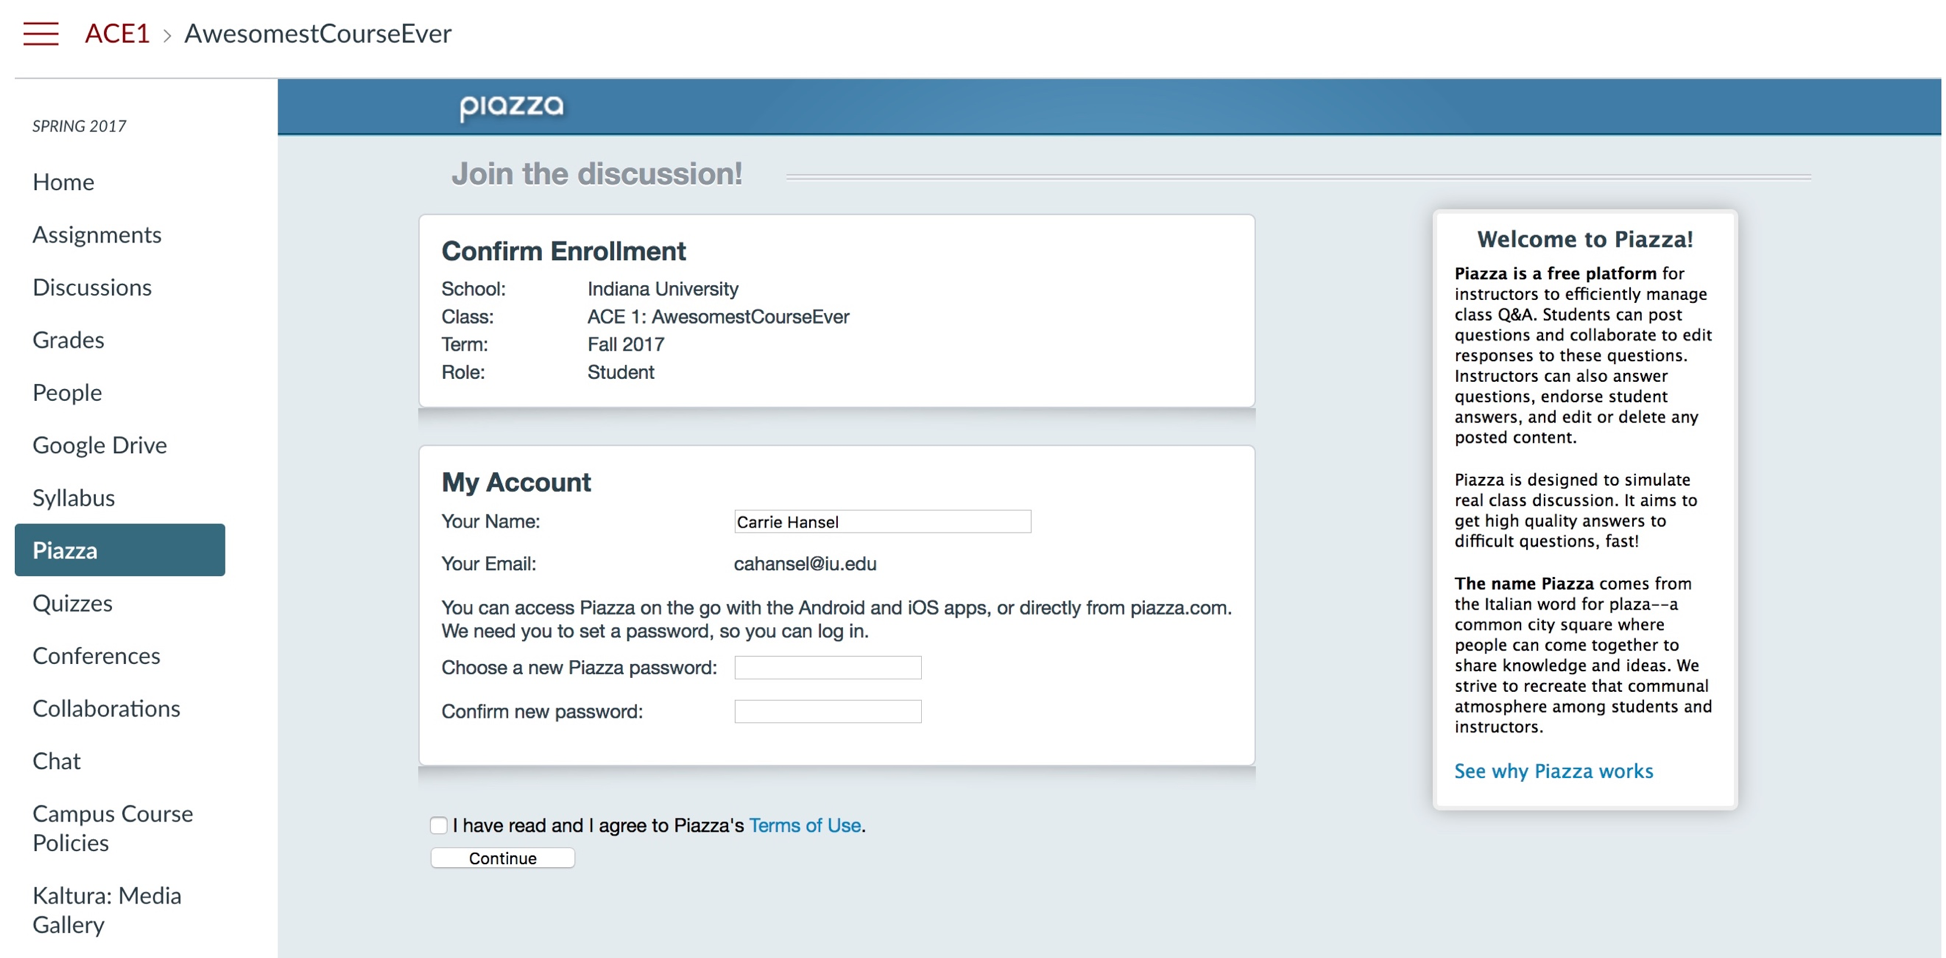
\includegraphics{images/image3.png}

Second, create password and accept terms.

\begin{description}
\item[The email address shown on this screen is your default IU]
email address. It is the address Canvas sends to all integrated tools
like Piazza. You can't edit it, so don't try.
\end{description}

\begin{description}
\item[The password you create here is for accessing Piazza from a]
mobile device. You must~use the default IU email address from this
screen to access this account on another device, so make a note of it.
\end{description}

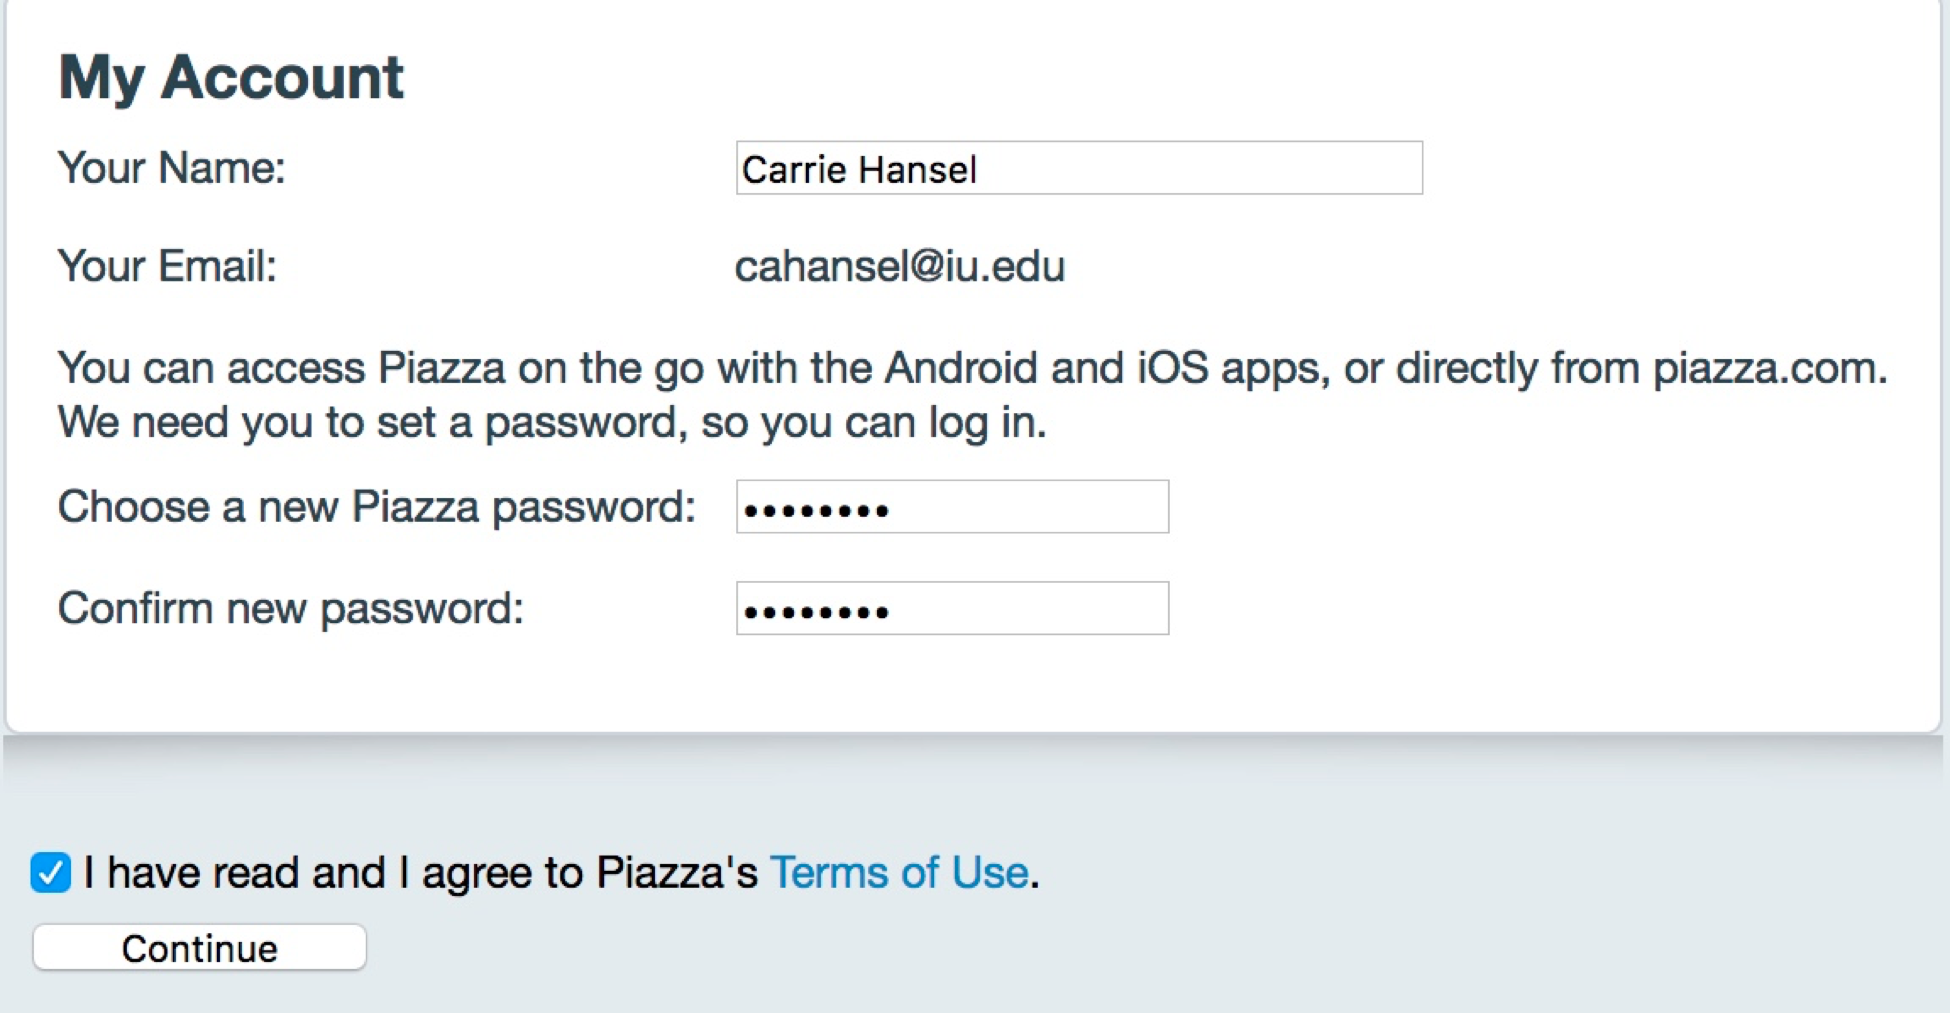
\includegraphics{images/image1.png}

Choose current degree program (only important if you want to opt into
their recruiting program on the next screen; choose whatever you want
here)

Third, associate your IU account

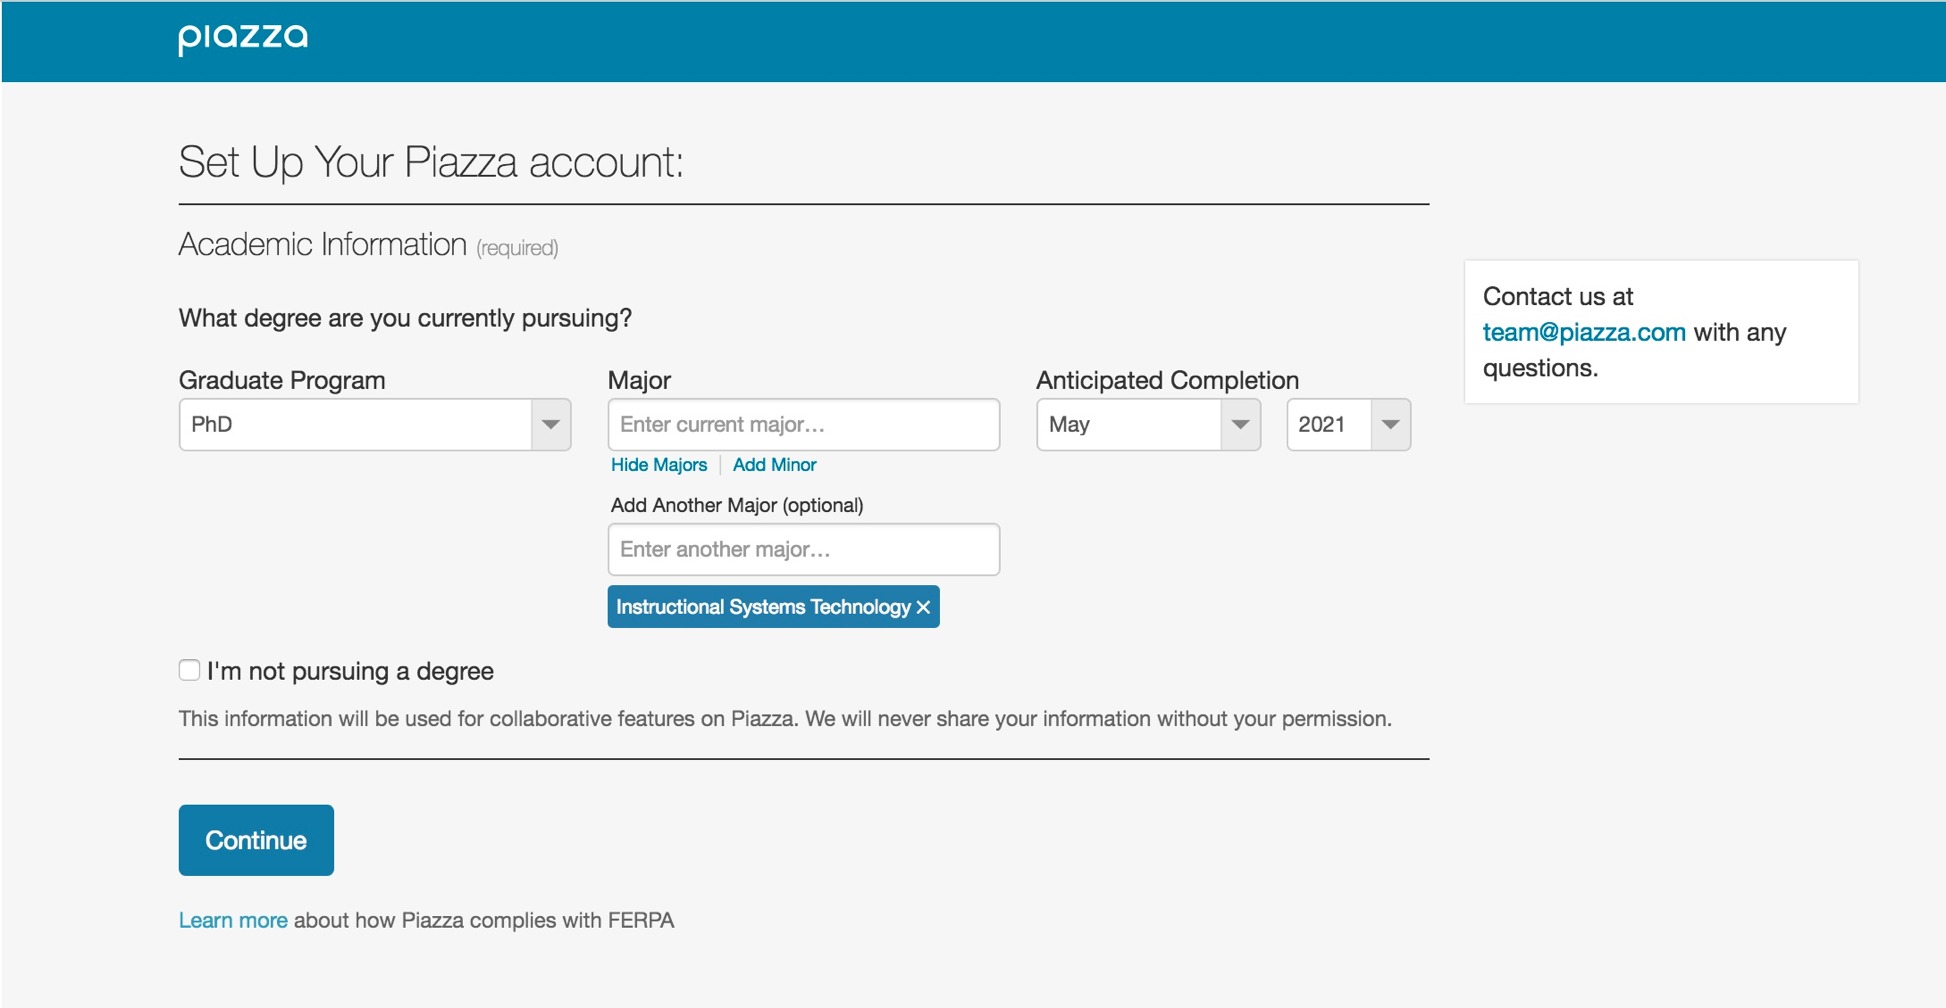
\includegraphics{images/image4.png}

Forth, if all goes well you see the Success screen

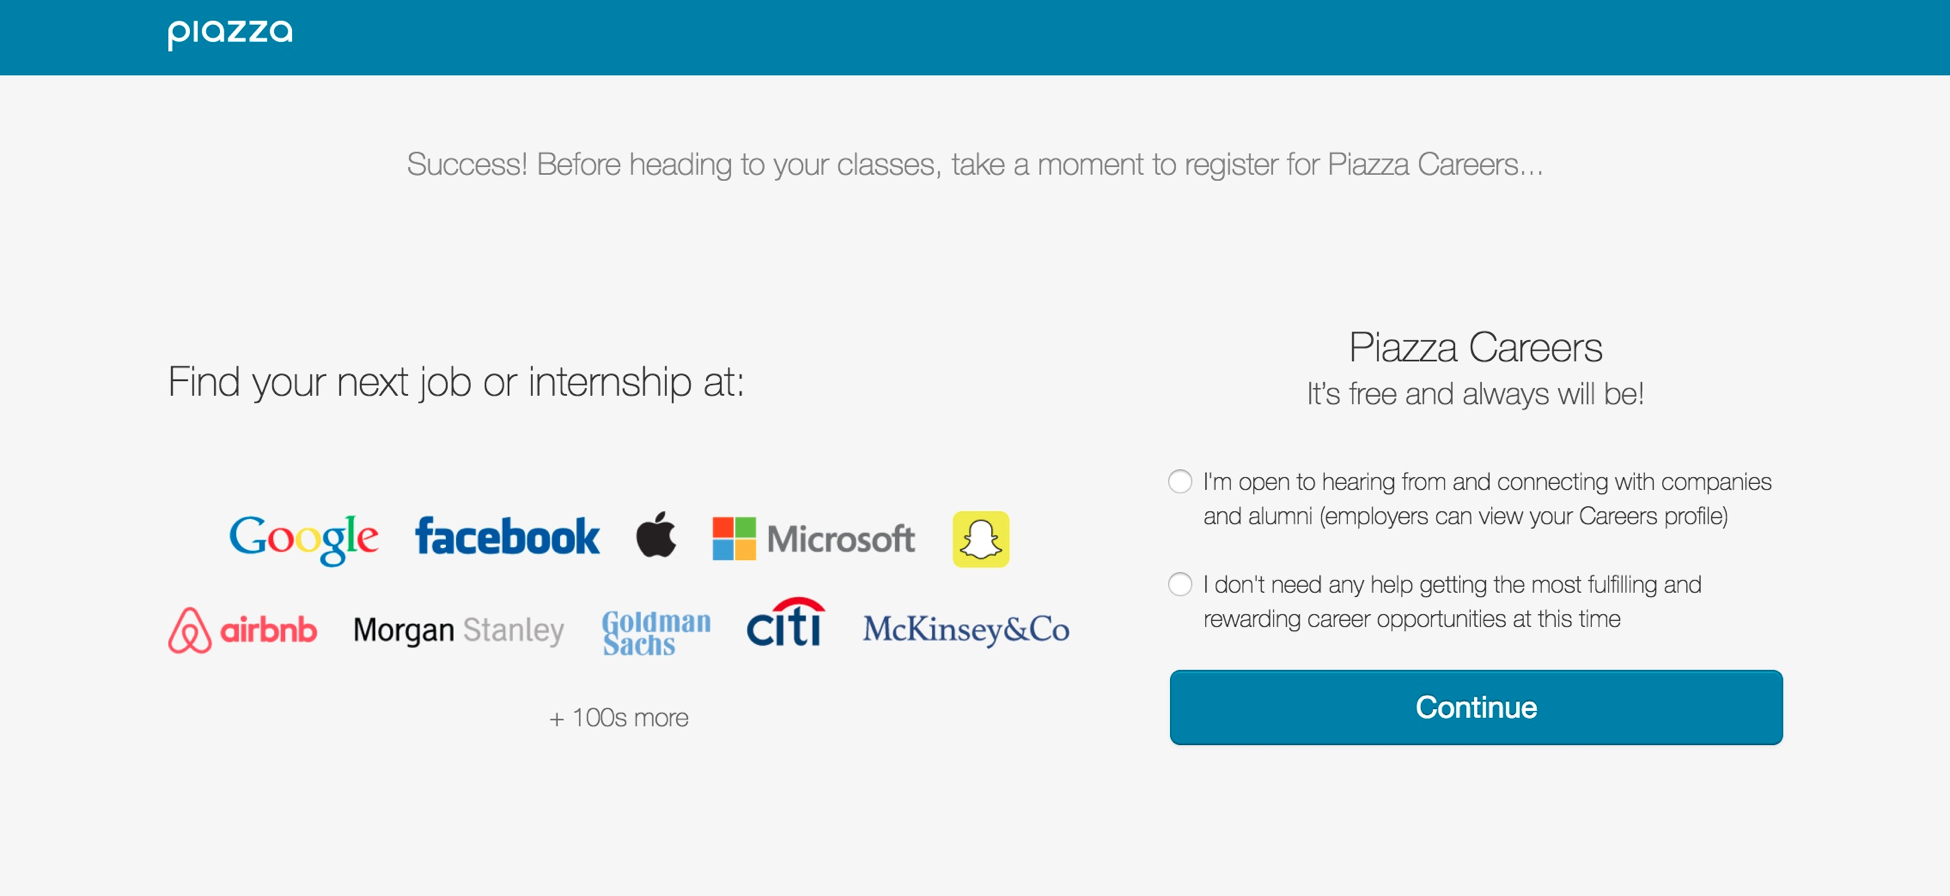
\includegraphics{images/image2.png}

\subsubsection{Situation: You have logged into piazza and used your
default IU
e-mail}\label{situation-you-have-logged-into-piazza-and-used-your-default-iu-e-mail}

\begin{enumerate}
\tightlist
\item
  Click the Piazza link on the left navigation of your Canvas course.
\item
  You will be automatically enrolled in the course Piazza site and
  logged in.
\item
  Start using Piazza.
\end{enumerate}

\subsubsection{Situation: You have logged into piazza and you used
another non IU
e-mail}\label{situation-you-have-logged-into-piazza-and-you-used-another-non-iu-e-mail}

\begin{enumerate}
\tightlist
\item
  Click the Piazza link on the left navigation of your Canvas course.
\item
  Proceed as in \#1 above. This will create your new Piazza account that
  is linked to your courses in Canvas. This is the account you should
  always use in your IU courses.
\item
  If you wish to merge other accounts that you own, please see
  \href{https://www.google.com/url?q=http://support.piazza.com/customer/portal/articles/1646661-add-an-email-address-or-merge-two-accounts\&sa=D\&ust=1502127148503000\&usg=AFQjCNHyBFh3TMAtSDpFordYOfH0IE6kPA}{Add
  an email address or merge two accounts}.
\end{enumerate}

\subsubsection{Situation: You have multiple accounts in
piazza}\label{situation-you-have-multiple-accounts-in-piazza}

\begin{enumerate}
\tightlist
\item
  If one of your multiple accounts corresponds with your default IU
  email address, you will be automatically enrolled in the course Piazza
  site and logged in.
\item
  If none of your accounts corresponds to your default IU email address,
  follow the instructions in \#3 above.
\item
  If you wish to merge other accounts that you own, please see
  \href{https://www.google.com/url?q=http://support.piazza.com/customer/portal/articles/1646661-add-an-email-address-or-merge-two-accounts\&sa=D\&ust=1502127148504000\&usg=AFQjCNHwO1kks2cnVLpWWCnOIEDFhl2fJA}{Add
  an email address or merge two accounts}.
\end{enumerate}

\begin{description}
\item[I post the official response form the CANVAS team here:]
``When a student clicks the Piazza link in your course navigation, they
will be authenticated through to Piazza. If the student already has a
Piazza account that matches their default Canvas email, they will simply
be enrolled in the Piazza course. If the student doesn't have an
account, Canvas sends the pertinent information (default email address
primarily) to Piazza, Piazza creates the student's account and enrolls
the student in the Piazza course. There is nothing you need to do to.''
\end{description}

If you have any questions regarding accessing piazza, please send them
to

``Ricci, Margaret P''
\textless{}\href{mailto:mricci@iu.edu}{\nolinkurl{mricci@iu.edu}}\textgreater{}

\subsection{Verify you are on Piazza via a
post}\label{verify-you-are-on-piazza-via-a-post}

Post on the \textbf{bio} folder a short introduction about yourself. One
that you could include in a paper.

An example is provided at \url{https://laszewski.github.io/bio.html}
with an image at \url{https://laszewski.github.io/_images/gregor.jpg}

Use the subject line \emph{Biography: Firstname Lastname} and post it
into the bio folder.

\subsection{Making Piazza Work}\label{making-piazza-work}

In order for Piazza to work students and instructors need to participate

\textbf{Students participate:} Students must collaboratively work on an
answer to a question. Students must not post irrelevant followups to a
question. If you notice your comment was irrelevant, please delete it.
Students must \textbf{search} prior to asking a new question if the
question has already been asked. Duplicated questions can be merged.

\textbf{Instructors guide:} The instructor guides the students in order
to obtain an answer to a question. In some cases the instructor may be
the only one knowing the answer in which case he tries to provide it.

\textbf{Not using e-mail:} Instructors will and must not use e-mail to
communicate with a student. All communication will be done via piazza.
There, are only very view situations where e-mail is allowed, ask on
piazza first if you should engage in e-mail conversations.

\textbf{Not using CANVAS discussions:} We will not engage in any CANVAS
message exchange. Any communication is to be done on Piazza. It is in
your responsibility to enroll in Piazza to make it work for you.
Instructions are posted in this document.

\subsection{Towards good questions}\label{towards-good-questions}

Naturally when you ask a question you need to do it in a reasonable form
and provide sufficient information so that the question can be answered.
It is in the responsibility of the student to update the question to
provide enough information.

Thus information may include: * Firstname * Lastname * PID * HID * URL
to document in question

To give you an example of a \textbf{bad} question consider:

\begin{verbatim}
*send from Xi Lee*

Hi Professor:

I read a nice article about apples and potato's and updated my
paper. Please give me feedback

Thank you

Kevin
\end{verbatim}

Here the reasons why this can be improved:

\begin{enumerate}
\def\labelenumi{\arabic{enumi}.}
\tightlist
\item
  As professors and instructors may review your document it is
  unnecessary to start with ``Hi Professor:'', just leave it away. If
  you want a particular instructor use the name explicitly, such as
  ``Gregor:'', e.g. multiple professors may be teaching your course.
\item
  You have not specified which article you read, you need to include the
  URL to the article so we can follow your argument.
\item
  You have not included the link to your document so we do not know what
  you are talking about. Remember there are many others students in the
  class
\item
  You are using a different name from the one that you are registered
  with. This can lead to confusion when we look up your name. We prefer
  that you use only one name that is associated with your e-mail.
\end{enumerate}

The above question will simply be commented on (if at all):

``Missing information'' or ``?'' indicating that information is missing.

\subsection{Guide on how to ask good
questions}\label{guide-on-how-to-ask-good-questions}

This guide is adapted from

\begin{itemize}
\tightlist
\item
  \url{http://www.techsupportalert.com/content/how-ask-question-when-you-want-technical-help.htm}
\end{itemize}

Ten steps to getting your question answered on piazza

\begin{enumerate}
\def\labelenumi{\arabic{enumi}.}
\tightlist
\item
  Before you even go to ask a question, think through what your problem
  is. Write down how you are going to describe it. Think about it from
  the other side - what would you need to know if a student came to you
  and asked the question? Gather all the system information that seems
  to bear on the problem (see how at this link). Sometimes it even
  happens that by thinking through the problem, you come up with the
  answer yourself.
\item
  Verify that your question has not yet been answered with a search on
  the Web, Class Web page, or class piazza, this may require multiple
  searches.
\item
  In case it is a technical question, write down any error codes that
  appear on your screen. do \textbf{not use screenshots} if the text is
  characters. This is because a reply my need to paste and copy from the
  original. Also screenshots are not searchable. We will not answer any
  questions that post screenshots if they are not necessary. It is far
  easier to copy and paste and use terminal type in the formatting. Also
  if the text is posted it is searchable. (Any unnecessary screenshot
  will receive a point deduction. Based on experience we have to do this
  as previous students in other classes ignored this policy).
\item
  Place your question or problem in a forum that is relevant to its
  subject. That may seem obvious but anyone who has experience with
  forums knows that a lot of questions show up in the wrong place. YOu
  will need to identify one or more a fitting piazza ``folders''
  (folders sort the posts by topics).
\item
  Select a title that briefly and accurately describes your problem. A
  title like ``Help!'' or ``Computer won't work'' will often get
  ignored. Almost any problem can be titled with a few key words that
  will raise interest in somebody who is familiar with the subject. A
  corollary to this is to avoid using all caps or a lot of exclamation
  points. Something like ``HELP!!!'' turns many people off.
\item
  In the post, briefly describe the problem in a paragraph. Leave out
  unnecessary details. Save everybody time by listing any solutions that
  you have tried but didn't work. Avoid using screenshots if they are
  not needed. (I mention this again).
\item
  IN case of a technical issue describe relevant system details. For
  example, it is essential to designate your operating system and type
  of computer and any components that might be involved in your problem.
  List any error code that has been displayed. Be prepared to provide
  more details if asked.
\item
  Tell what you were doing when you encountered the problem. If it is a
  reproducible problem, list the steps or computer operations that cause
  the problem.
\item
  If applicable, List any recent software you have installed or hardware
  changes you have made. If you have updated any drivers recently, also
  list that.
\item
  Formulate your questions and answers in a courteous manner. Respect
  the answers from others. Somebody is giving you their time and
  expertise for free. You may want to come back to the forum and it pays
  to be friendly.
\item
  If a suggested solution works, be sure to return to piazza and report
  your success. It is the least you can do to return something for the
  help you have been given. It will make you welcome in the forum the
  next time you go there for help.
\end{enumerate}

\subsection{Piazza class Links}\label{piazza-class-links}

\begin{description}
\item[Using the following direct links can lead to you not]
getting proper access via Canvas. If you click on these links
\textbf{before they create} the account via the link in your current
Canvas course, you will create an account that is not matched up with
Canvas.
\end{description}

To avoid issues make sure you integrate to piazza via Canvas first.

If you have questions bout this contact Margaret Ricci.

Classes hosted on Piazza

\begin{itemize}
\tightlist
\item
  Fall 2017:

  \begin{itemize}
  \tightlist
  \item
    I523: \url{https://piazza.com/iu/fall2017/i523/home}
  \end{itemize}
\end{itemize}

Older Classes

\begin{itemize}
\tightlist
\item
  I524 Spring 2017: \url{https://piazza.com/class/ix39m27czn5uw}
\item
  I523 Fall 2016: \url{https://piazza.com/class/irqfvh1ctrg2vt}
\end{itemize}

\subsection{Piazza Curration for I523}\label{piazza-curration-for-i523}

We are using Piazza in a currated fashion and we like that all students
participate in this. This will allow Piazza to become a superior tool
for all in the class. IN general we only allow \textbf{exactly one
folder} for a message. If a message is wrongly filed it will be
corrected, either by students or TAs.

As part of this we are intrducing anumber of folders. Some of which must
not be used by students. We list the folllowing folders and their
purpose:

\begin{description}
\item[logistics:]
Any question and discussion related to the logistics of the course
\item[lectures:]
Any question and discussion related to the lectures.
\item[p1:]
Any question and discussion related to paper 1.
\item[p2:]
Any question and discussion related to paper 2.
\item[proj-iot:]
Any question and discussion related to iot projects.
\item[proj-term:]
Any question and discussion related to the term project.
\item[python:]
Any question and discussion related to python.
\item[pi:]
Any question and discussion related to the Raspberry Pi 3. We are not
using older Raspberry Pi's and therefore can not comment to them.
\item[8266:]
Any question and discussion related to the esp8266.
\item[bio:]
A homework folder in which you only publish your bio. The bio needs to
be published as a \emph{note}. This assignment also serves us to see if
you are in piazza. Please do this assignment ASSAP. You need to post a
formal bio. See the many great examples in the folder.
\item[help:]
If you need help and none of the other folders fits, please use this
folder. If information from here will result into new Web page content
it will be added and marked into the folder \emph{resolved}. See the
\emph{resolved} folder for more detail.
\item[resolved:]
Sometimes we move some general help messages to the resolved folder in
case the help message results into information that is posted on our
class Web page. We than will add a link to where in the class Web page
this question was answered. The TAs will aggressively try to put
information into the Web page.
\item[discussion:]
Any content that deserves its seperate discussion and is not covered in
the above folder.
\end{description}

In addition to these general folders we also have two folders which
\textbf{MUST NOT BE USED BY ANY STUDENT TO POST CONTENT}. These folders
serve to communicate your assignments and are used internally between
Grgeor and the TA's.

\begin{description}
\item[\emph{assignments}:]
This folder only lists the assignments. At any time in the class you can
click on the assignment folder and list the assignments given to the
class. THus there is no confusion which assignments have been given. In
case students have questions about assignments they should not use the
\emph{assignments} folder, but the \emph{help} folder. TAs are
instructed to correct wrongly filed messages in folders.
\item[\emph{ta}:]
Any question and discussion you have for the ta's. Typically you should
however use the folder \emph{help}. Gregor use most often the \emph{ta}
folder for internal coordination with the tas.
\end{description}

It may be necessary to create new folders for the class. Their meeing
will be updated here once this occurs.

In case you decide to post privately and the information is useful for
others also, the message will be published to the class.

A convenient post with all folders that are useful to know is posted at:

\begin{itemize}
\tightlist
\item
  \url{https://piazza.com/class/j5wll7vzylg25j?cid=103}
\end{itemize}

If you click on the foldername, you can see all posts in that folder.

\subsection{Video about i523 Piazza}\label{video-about-i523-piazza}

A video on how piazzza is used in i523 is shown at:

\begin{itemize}
\tightlist
\item
  \url{https://youtu.be/9hnW-327CMQ}
\end{itemize}

\subsection{Exercise}\label{exercise}

\begin{description}
\item[EPiazza.1:]
Enroll in piazza
\item[EPiazza.2:]
Post a short formal bio in the bio folder (optionally include a
professional portrait of yourself). Make sure you understand what a
formal bio is.
\item[EPiazza.3:]
How do you find out within Piazza which assignments have been posted?
\item[EPiazza.4:]
Please watch the Video about i523 Piazza
\end{description}


%\FILENAME

\section{Piazza}\label{piazza}

We use Piazza (\url{https://piazza.com}) because questions and answers
on Piazza are community-edited. Each question has a single answer edited
by the students of the class and if needed an instructors' answer that
is collaboratively edited by the instructors.

Due to this wiki-style Q\&A, when a student has a question, one does not
have to look through long e-mail threads but instead can look at the
answer. For details that lead up to the answer you are highly encouraged
to also look at some comments that lead up to the answer

An advertisement video from Piazza summarizes the features:

\begin{itemize}
\tightlist
\item
  \url{https://www.youtube.com/watch?v=2jLSiN8E18w}
\end{itemize}

Piazza Support with a lot of information is available at:

\begin{itemize}
\tightlist
\item
  \url{http://support.piazza.com}
\end{itemize}

\subsection{Access to Piazza from
Canvas}\label{access-to-piazza-from-canvas}

Piazza is one of the recommended IU supported technologies within
Canvas. It replaces the CANVAS discussion groups with superior
technology targeted to support large student classes while also
focussing on student engagement.

To access piazza you can have the following situations provided in the
next four subsections. PLease read \emph{ALL}* of them
\textbf{CAREFULLY}, decide which applies tou you and follow the
instructions. If you have imporvements to this instructions, please let
us know.

\subsubsection{Situation: You have never logged into
piazza}\label{situation-you-have-never-logged-into-piazza}

First, Click the Piazza link on the left navigation of your Canvas
course.

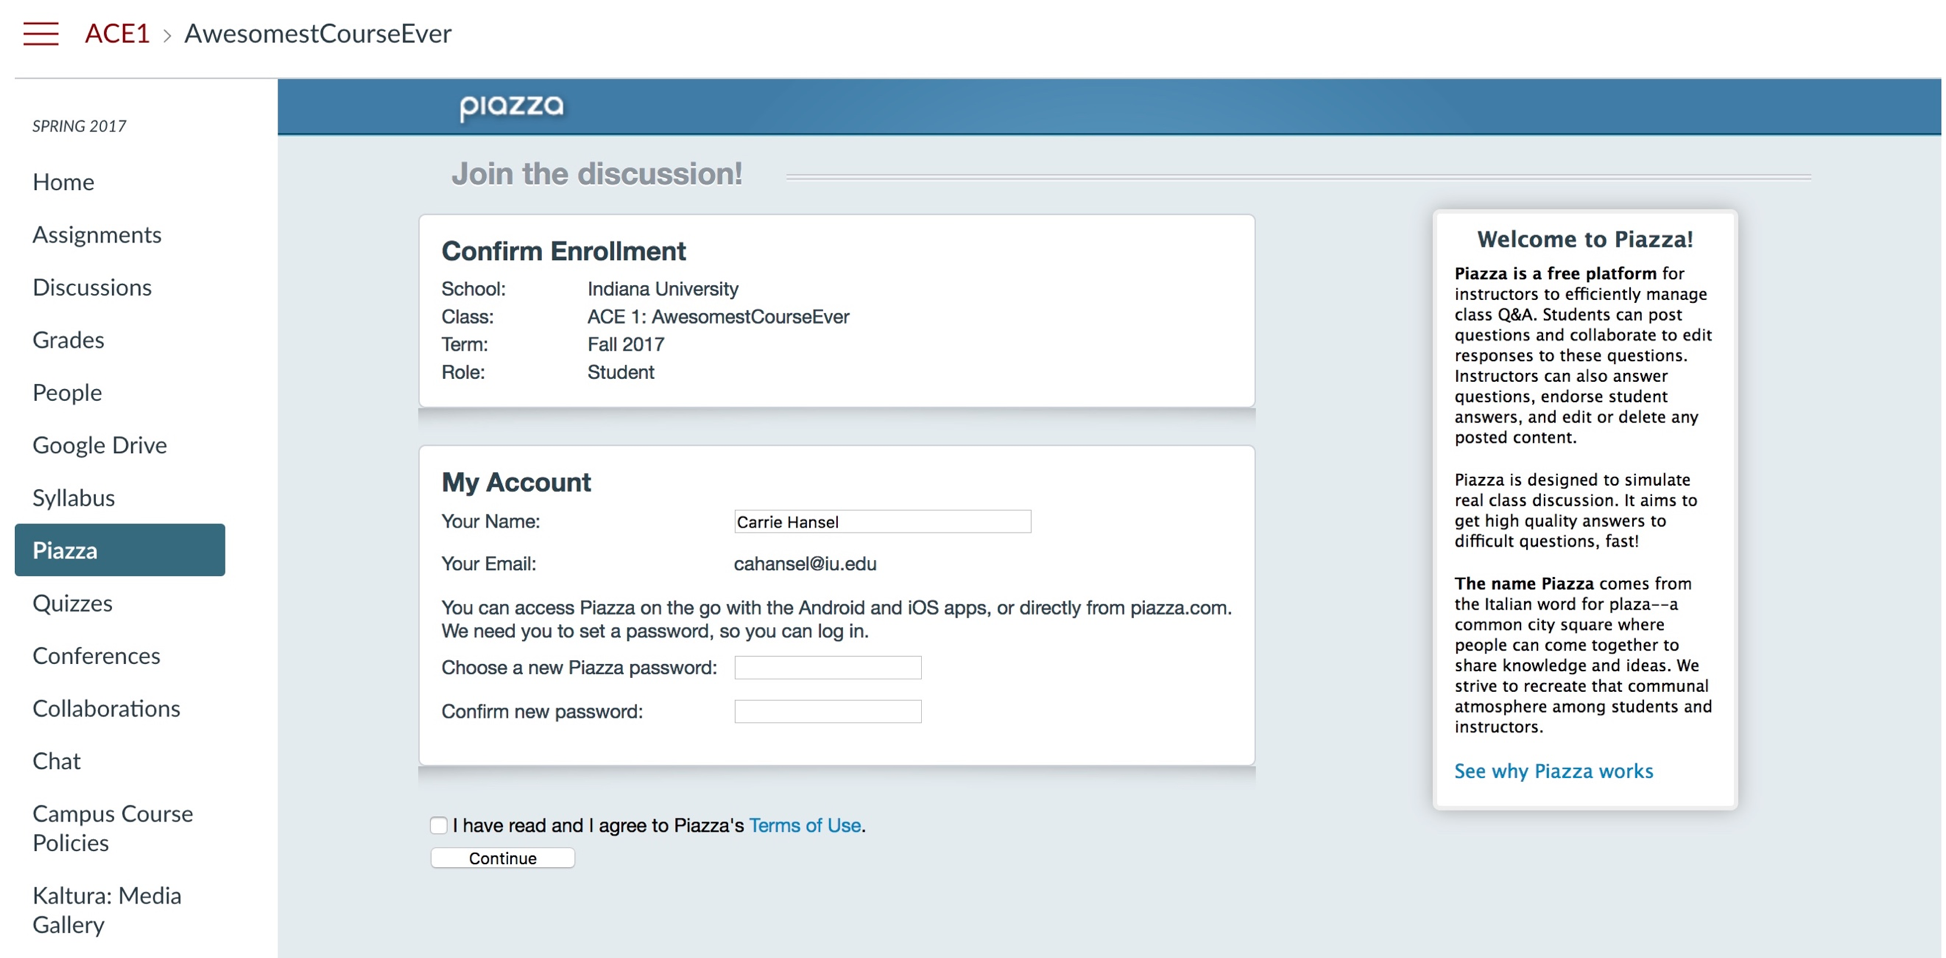
\includegraphics{images/image3.png}

Second, create password and accept terms.

\begin{description}
\item[The email address shown on this screen is your default IU]
email address. It is the address Canvas sends to all integrated tools
like Piazza. You can't edit it, so don't try.
\end{description}

\begin{description}
\item[The password you create here is for accessing Piazza from a]
mobile device. You must~use the default IU email address from this
screen to access this account on another device, so make a note of it.
\end{description}

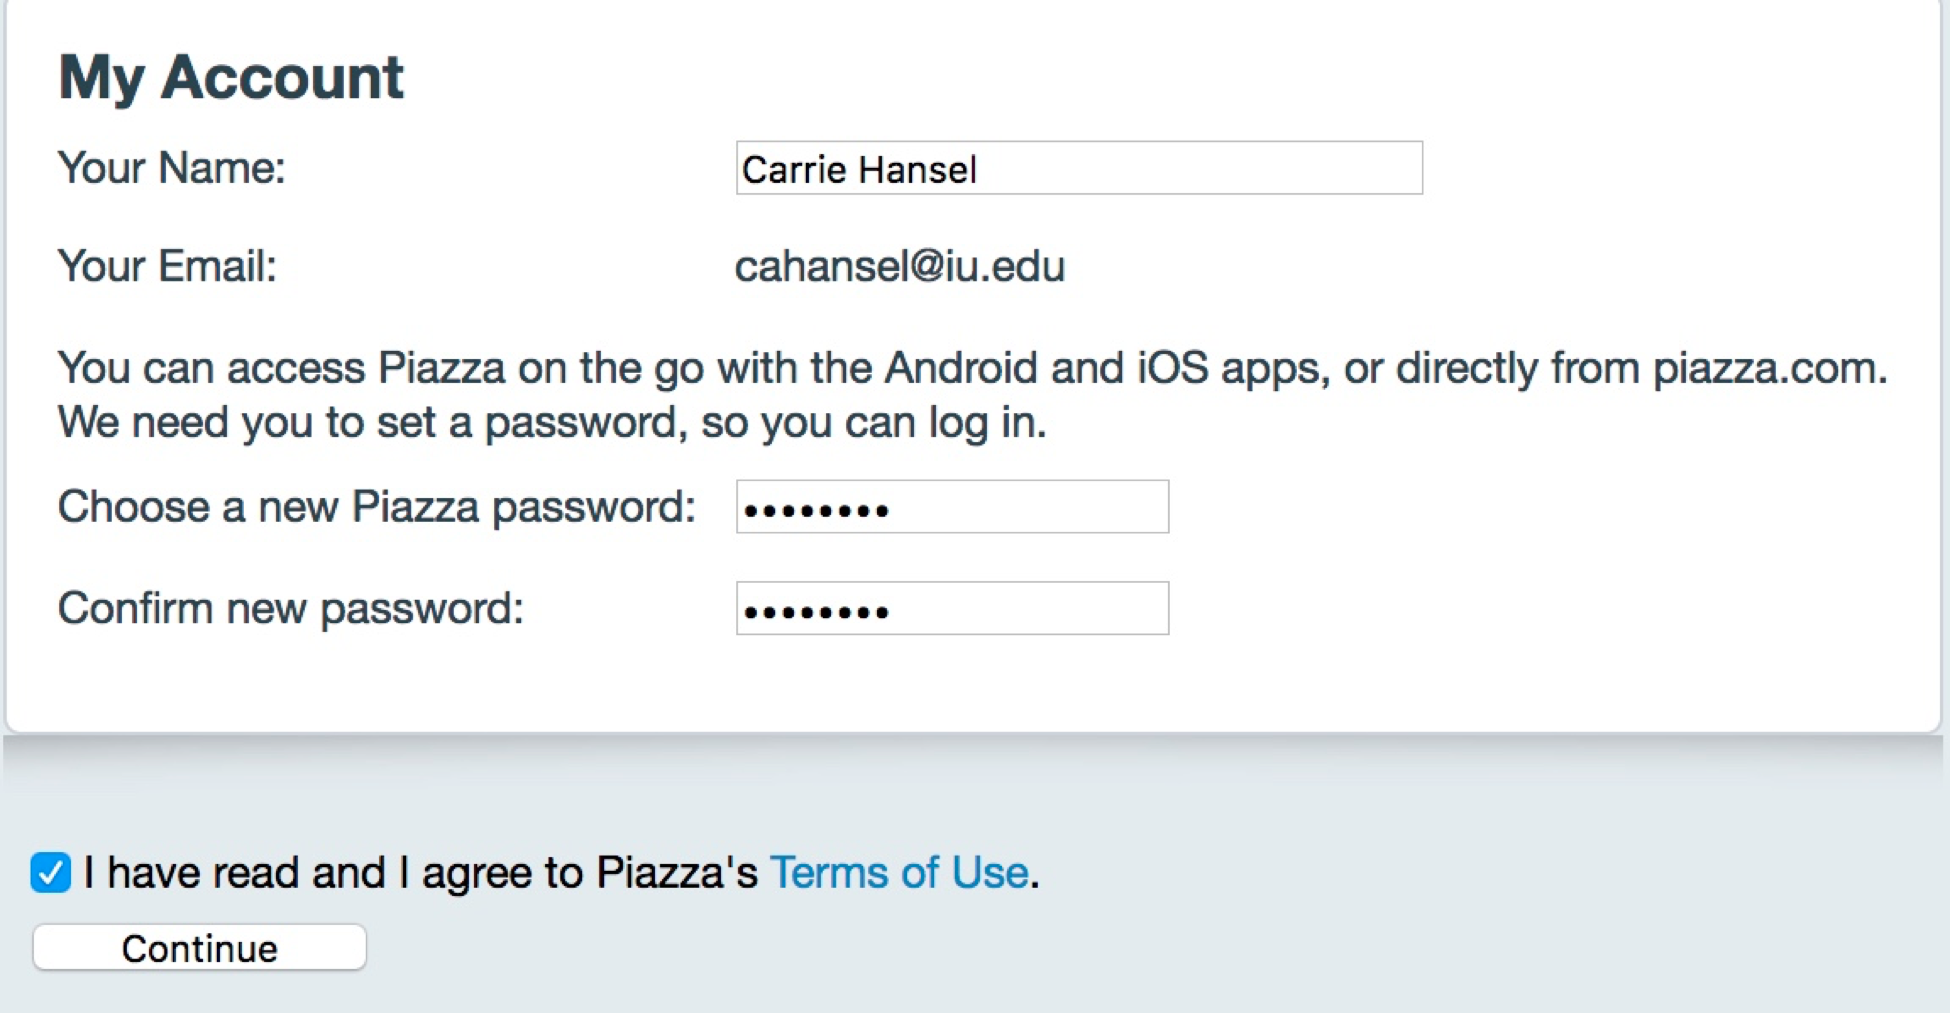
\includegraphics{images/image1.png}

Choose current degree program (only important if you want to opt into
their recruiting program on the next screen; choose whatever you want
here)

Third, associate your IU account

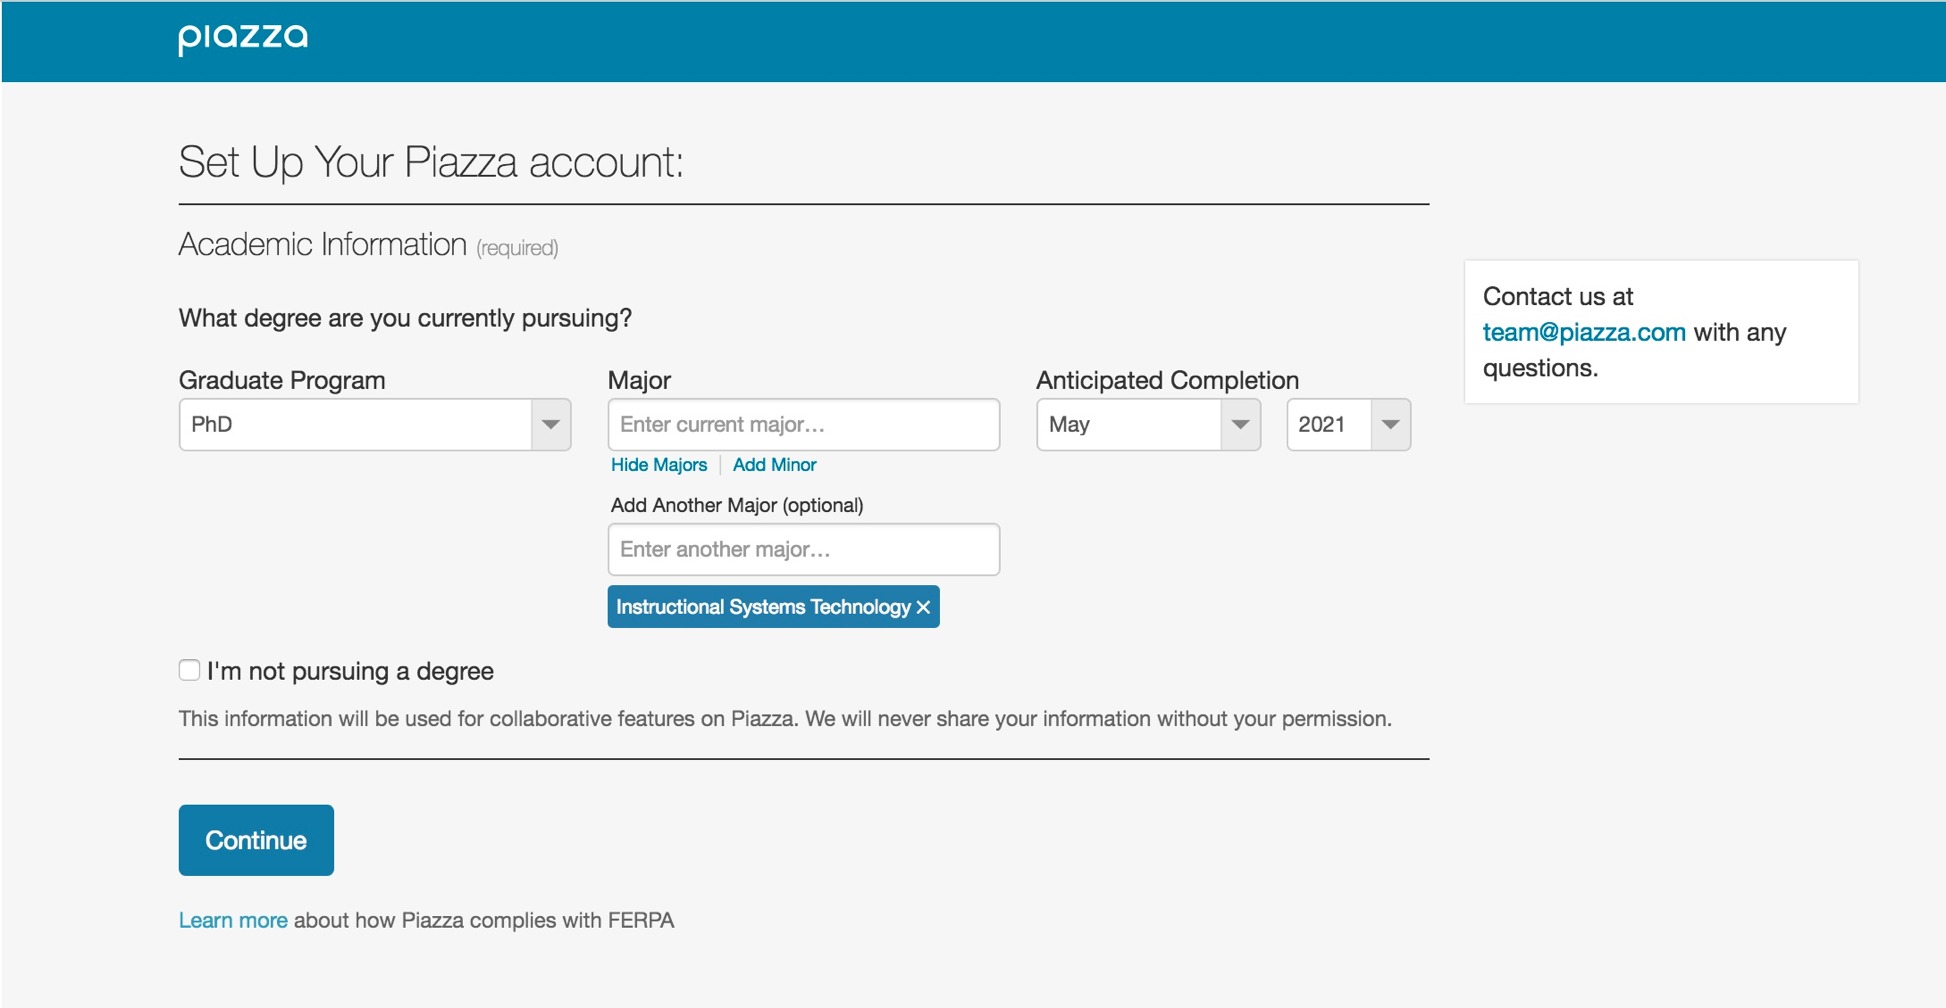
\includegraphics{images/image4.png}

Forth, if all goes well you see the Success screen

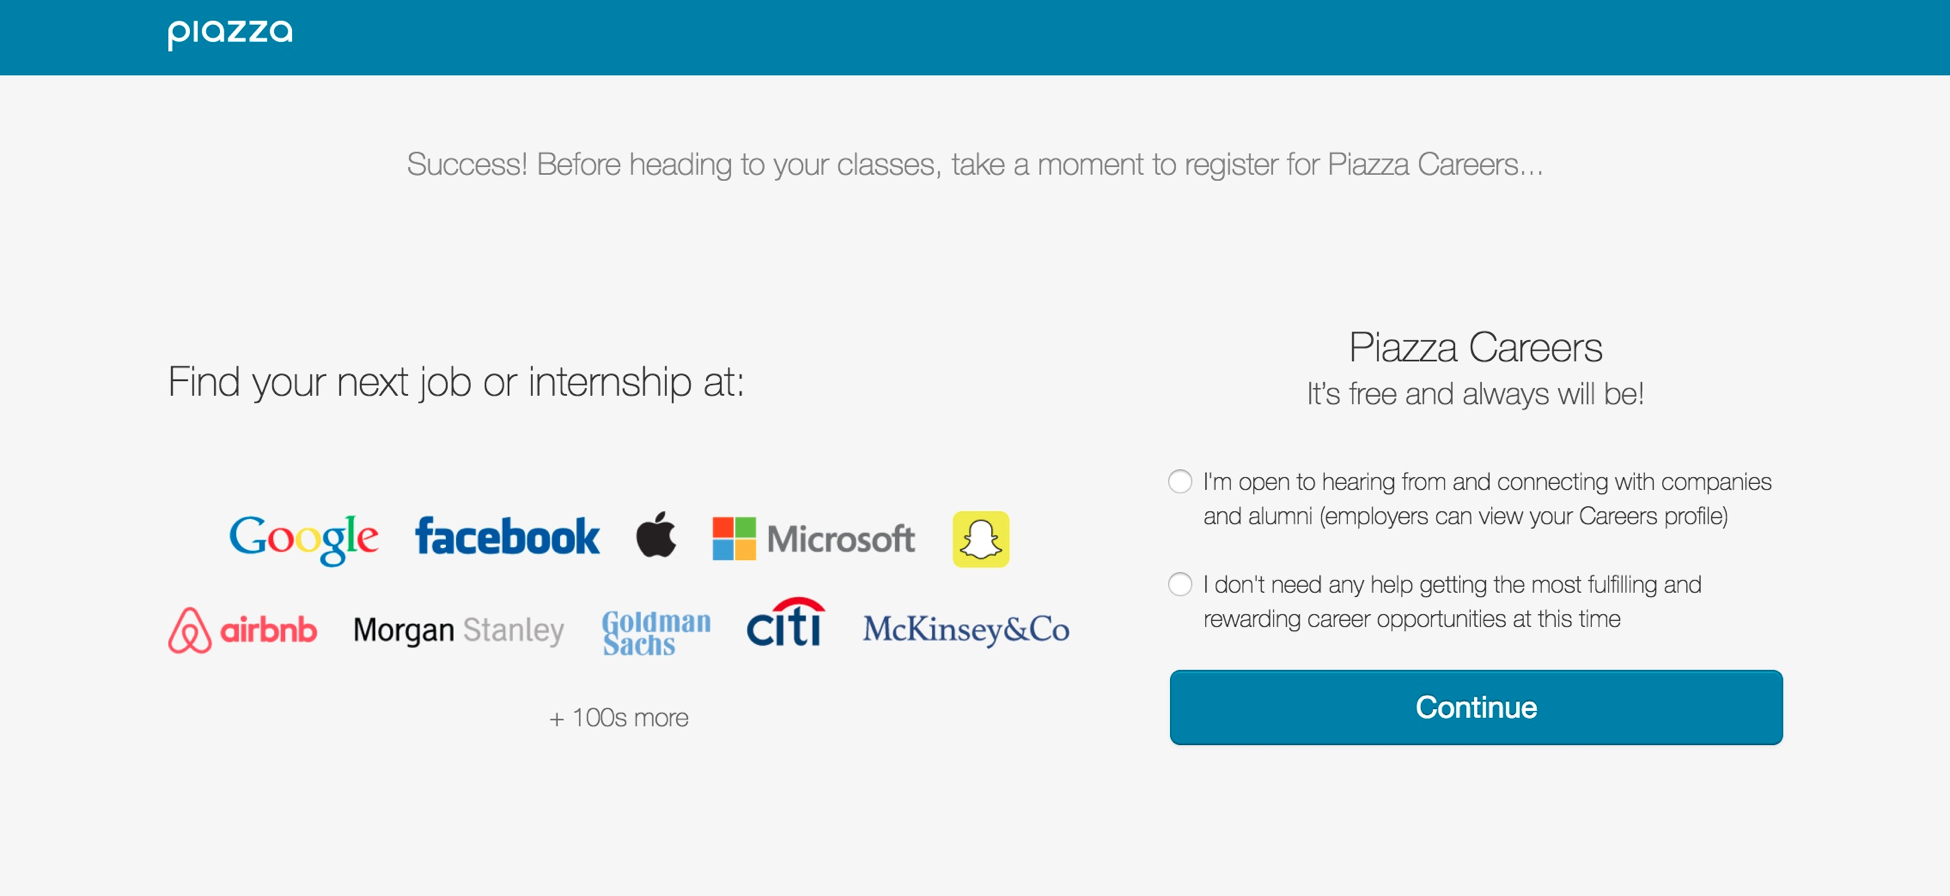
\includegraphics{images/image2.png}

\subsubsection{Situation: You have logged into piazza and used your
default IU
e-mail}\label{situation-you-have-logged-into-piazza-and-used-your-default-iu-e-mail}

\begin{enumerate}
\tightlist
\item
  Click the Piazza link on the left navigation of your Canvas course.
\item
  You will be automatically enrolled in the course Piazza site and
  logged in.
\item
  Start using Piazza.
\end{enumerate}

\subsubsection{Situation: You have logged into piazza and you used
another non IU
e-mail}\label{situation-you-have-logged-into-piazza-and-you-used-another-non-iu-e-mail}

\begin{enumerate}
\tightlist
\item
  Click the Piazza link on the left navigation of your Canvas course.
\item
  Proceed as in \#1 above. This will create your new Piazza account that
  is linked to your courses in Canvas. This is the account you should
  always use in your IU courses.
\item
  If you wish to merge other accounts that you own, please see
  \href{https://www.google.com/url?q=http://support.piazza.com/customer/portal/articles/1646661-add-an-email-address-or-merge-two-accounts\&sa=D\&ust=1502127148503000\&usg=AFQjCNHyBFh3TMAtSDpFordYOfH0IE6kPA}{Add
  an email address or merge two accounts}.
\end{enumerate}

\subsubsection{Situation: You have multiple accounts in
piazza}\label{situation-you-have-multiple-accounts-in-piazza}

\begin{enumerate}
\tightlist
\item
  If one of your multiple accounts corresponds with your default IU
  email address, you will be automatically enrolled in the course Piazza
  site and logged in.
\item
  If none of your accounts corresponds to your default IU email address,
  follow the instructions in \#3 above.
\item
  If you wish to merge other accounts that you own, please see
  \href{https://www.google.com/url?q=http://support.piazza.com/customer/portal/articles/1646661-add-an-email-address-or-merge-two-accounts\&sa=D\&ust=1502127148504000\&usg=AFQjCNHwO1kks2cnVLpWWCnOIEDFhl2fJA}{Add
  an email address or merge two accounts}.
\end{enumerate}

\begin{description}
\item[I post the official response form the CANVAS team here:]
``When a student clicks the Piazza link in your course navigation, they
will be authenticated through to Piazza. If the student already has a
Piazza account that matches their default Canvas email, they will simply
be enrolled in the Piazza course. If the student doesn't have an
account, Canvas sends the pertinent information (default email address
primarily) to Piazza, Piazza creates the student's account and enrolls
the student in the Piazza course. There is nothing you need to do to.''
\end{description}

If you have any questions regarding accessing piazza, please send them
to

``Ricci, Margaret P''
\textless{}\href{mailto:mricci@iu.edu}{\nolinkurl{mricci@iu.edu}}\textgreater{}

\subsection{Verify you are on Piazza via a
post}\label{verify-you-are-on-piazza-via-a-post}

Post on the \textbf{bio} folder a short introduction about yourself. One
that you could include in a paper.

An example is provided at \url{https://laszewski.github.io/bio.html}
with an image at \url{https://laszewski.github.io/_images/gregor.jpg}

Use the subject line \emph{Biography: Firstname Lastname} and post it
into the bio folder.

\subsection{Making Piazza Work}\label{making-piazza-work}

In order for Piazza to work students and instructors need to participate

\textbf{Students participate:} Students must collaboratively work on an
answer to a question. Students must not post irrelevant followups to a
question. If you notice your comment was irrelevant, please delete it.
Students must \textbf{search} prior to asking a new question if the
question has already been asked. Duplicated questions can be merged.

\textbf{Instructors guide:} The instructor guides the students in order
to obtain an answer to a question. In some cases the instructor may be
the only one knowing the answer in which case he tries to provide it.

\textbf{Not using e-mail:} Instructors will and must not use e-mail to
communicate with a student. All communication will be done via piazza.
There, are only very view situations where e-mail is allowed, ask on
piazza first if you should engage in e-mail conversations.

\textbf{Not using CANVAS discussions:} We will not engage in any CANVAS
message exchange. Any communication is to be done on Piazza. It is in
your responsibility to enroll in Piazza to make it work for you.
Instructions are posted in this document.

\subsection{Towards good questions}\label{towards-good-questions}

Naturally when you ask a question you need to do it in a reasonable form
and provide sufficient information so that the question can be answered.
It is in the responsibility of the student to update the question to
provide enough information.

Thus information may include: * Firstname * Lastname * PID * HID * URL
to document in question

To give you an example of a \textbf{bad} question consider:

\begin{verbatim}
*send from Xi Lee*

Hi Professor:

I read a nice article about apples and potato's and updated my
paper. Please give me feedback

Thank you

Kevin
\end{verbatim}

Here the reasons why this can be improved:

\begin{enumerate}
\def\labelenumi{\arabic{enumi}.}
\tightlist
\item
  As professors and instructors may review your document it is
  unnecessary to start with ``Hi Professor:'', just leave it away. If
  you want a particular instructor use the name explicitly, such as
  ``Gregor:'', e.g. multiple professors may be teaching your course.
\item
  You have not specified which article you read, you need to include the
  URL to the article so we can follow your argument.
\item
  You have not included the link to your document so we do not know what
  you are talking about. Remember there are many others students in the
  class
\item
  You are using a different name from the one that you are registered
  with. This can lead to confusion when we look up your name. We prefer
  that you use only one name that is associated with your e-mail.
\end{enumerate}

The above question will simply be commented on (if at all):

``Missing information'' or ``?'' indicating that information is missing.

\subsection{Guide on how to ask good
questions}\label{guide-on-how-to-ask-good-questions}

This guide is adapted from

\begin{itemize}
\tightlist
\item
  \url{http://www.techsupportalert.com/content/how-ask-question-when-you-want-technical-help.htm}
\end{itemize}

Ten steps to getting your question answered on piazza

\begin{enumerate}
\def\labelenumi{\arabic{enumi}.}
\tightlist
\item
  Before you even go to ask a question, think through what your problem
  is. Write down how you are going to describe it. Think about it from
  the other side - what would you need to know if a student came to you
  and asked the question? Gather all the system information that seems
  to bear on the problem (see how at this link). Sometimes it even
  happens that by thinking through the problem, you come up with the
  answer yourself.
\item
  Verify that your question has not yet been answered with a search on
  the Web, Class Web page, or class piazza, this may require multiple
  searches.
\item
  In case it is a technical question, write down any error codes that
  appear on your screen. do \textbf{not use screenshots} if the text is
  characters. This is because a reply my need to paste and copy from the
  original. Also screenshots are not searchable. We will not answer any
  questions that post screenshots if they are not necessary. It is far
  easier to copy and paste and use terminal type in the formatting. Also
  if the text is posted it is searchable. (Any unnecessary screenshot
  will receive a point deduction. Based on experience we have to do this
  as previous students in other classes ignored this policy).
\item
  Place your question or problem in a forum that is relevant to its
  subject. That may seem obvious but anyone who has experience with
  forums knows that a lot of questions show up in the wrong place. YOu
  will need to identify one or more a fitting piazza ``folders''
  (folders sort the posts by topics).
\item
  Select a title that briefly and accurately describes your problem. A
  title like ``Help!'' or ``Computer won't work'' will often get
  ignored. Almost any problem can be titled with a few key words that
  will raise interest in somebody who is familiar with the subject. A
  corollary to this is to avoid using all caps or a lot of exclamation
  points. Something like ``HELP!!!'' turns many people off.
\item
  In the post, briefly describe the problem in a paragraph. Leave out
  unnecessary details. Save everybody time by listing any solutions that
  you have tried but didn't work. Avoid using screenshots if they are
  not needed. (I mention this again).
\item
  IN case of a technical issue describe relevant system details. For
  example, it is essential to designate your operating system and type
  of computer and any components that might be involved in your problem.
  List any error code that has been displayed. Be prepared to provide
  more details if asked.
\item
  Tell what you were doing when you encountered the problem. If it is a
  reproducible problem, list the steps or computer operations that cause
  the problem.
\item
  If applicable, List any recent software you have installed or hardware
  changes you have made. If you have updated any drivers recently, also
  list that.
\item
  Formulate your questions and answers in a courteous manner. Respect
  the answers from others. Somebody is giving you their time and
  expertise for free. You may want to come back to the forum and it pays
  to be friendly.
\item
  If a suggested solution works, be sure to return to piazza and report
  your success. It is the least you can do to return something for the
  help you have been given. It will make you welcome in the forum the
  next time you go there for help.
\end{enumerate}

\subsection{Piazza class Links}\label{piazza-class-links}

\begin{description}
\item[Using the following direct links can lead to you not]
getting proper access via Canvas. If you click on these links
\textbf{before they create} the account via the link in your current
Canvas course, you will create an account that is not matched up with
Canvas.
\end{description}

To avoid issues make sure you integrate to piazza via Canvas first.

If you have questions bout this contact Margaret Ricci.

Classes hosted on Piazza

\begin{itemize}
\tightlist
\item
  Fall 2017:

  \begin{itemize}
  \tightlist
  \item
    I523: \url{https://piazza.com/iu/fall2017/i523/home}
  \end{itemize}
\end{itemize}

Older Classes

\begin{itemize}
\tightlist
\item
  I524 Spring 2017: \url{https://piazza.com/class/ix39m27czn5uw}
\item
  I523 Fall 2016: \url{https://piazza.com/class/irqfvh1ctrg2vt}
\end{itemize}

\subsection{Piazza Curration for I523}\label{piazza-curration-for-i523}

We are using Piazza in a currated fashion and we like that all students
participate in this. This will allow Piazza to become a superior tool
for all in the class. IN general we only allow \textbf{exactly one
folder} for a message. If a message is wrongly filed it will be
corrected, either by students or TAs.

As part of this we are intrducing anumber of folders. Some of which must
not be used by students. We list the folllowing folders and their
purpose:

\begin{description}
\item[logistics:]
Any question and discussion related to the logistics of the course
\item[lectures:]
Any question and discussion related to the lectures.
\item[p1:]
Any question and discussion related to paper 1.
\item[p2:]
Any question and discussion related to paper 2.
\item[proj-iot:]
Any question and discussion related to iot projects.
\item[proj-term:]
Any question and discussion related to the term project.
\item[python:]
Any question and discussion related to python.
\item[pi:]
Any question and discussion related to the Raspberry Pi 3. We are not
using older Raspberry Pi's and therefore can not comment to them.
\item[8266:]
Any question and discussion related to the esp8266.
\item[bio:]
A homework folder in which you only publish your bio. The bio needs to
be published as a \emph{note}. This assignment also serves us to see if
you are in piazza. Please do this assignment ASSAP. You need to post a
formal bio. See the many great examples in the folder.
\item[help:]
If you need help and none of the other folders fits, please use this
folder. If information from here will result into new Web page content
it will be added and marked into the folder \emph{resolved}. See the
\emph{resolved} folder for more detail.
\item[resolved:]
Sometimes we move some general help messages to the resolved folder in
case the help message results into information that is posted on our
class Web page. We than will add a link to where in the class Web page
this question was answered. The TAs will aggressively try to put
information into the Web page.
\item[discussion:]
Any content that deserves its seperate discussion and is not covered in
the above folder.
\end{description}

In addition to these general folders we also have two folders which
\textbf{MUST NOT BE USED BY ANY STUDENT TO POST CONTENT}. These folders
serve to communicate your assignments and are used internally between
Grgeor and the TA's.

\begin{description}
\item[\emph{assignments}:]
This folder only lists the assignments. At any time in the class you can
click on the assignment folder and list the assignments given to the
class. THus there is no confusion which assignments have been given. In
case students have questions about assignments they should not use the
\emph{assignments} folder, but the \emph{help} folder. TAs are
instructed to correct wrongly filed messages in folders.
\item[\emph{ta}:]
Any question and discussion you have for the ta's. Typically you should
however use the folder \emph{help}. Gregor use most often the \emph{ta}
folder for internal coordination with the tas.
\end{description}

It may be necessary to create new folders for the class. Their meeing
will be updated here once this occurs.

In case you decide to post privately and the information is useful for
others also, the message will be published to the class.

A convenient post with all folders that are useful to know is posted at:

\begin{itemize}
\tightlist
\item
  \url{https://piazza.com/class/j5wll7vzylg25j?cid=103}
\end{itemize}

If you click on the foldername, you can see all posts in that folder.

\subsection{Video about i523 Piazza}\label{video-about-i523-piazza}

A video on how piazzza is used in i523 is shown at:

\begin{itemize}
\tightlist
\item
  \url{https://youtu.be/9hnW-327CMQ}
\end{itemize}

\subsection{Exercise}\label{exercise}

\begin{description}
\item[EPiazza.1:]
Enroll in piazza
\item[EPiazza.2:]
Post a short formal bio in the bio folder (optionally include a
professional portrait of yourself). Make sure you understand what a
formal bio is.
\item[EPiazza.3:]
How do you find out within Piazza which assignments have been posted?
\item[EPiazza.4:]
Please watch the Video about i523 Piazza
\end{description}




% BIG DATA APPLICATIONS


%-------------------------------------------------------------------------------
%	PART
%-------------------------------------------------------------------------------

\part{Big Data Applications}

\FILENAME

\FILENAME

\section{Introduction}\label{introduction}

\begin{description}
\item[You may find that some videos may have a different lesson,]
section or unit number. Please ignore this. In case the content does not
correspond to the title, please let us know.
\end{description}

This section has a technical overview of course followed by a broad
motivation for course hosted at www-cloudmesh-classes.

The course overview covers it's content and structure. It presents an
introduction to general field of Big Data and Analytics. We are
especially analysing the many different application areas in which Big
Data can be applied. As Big Datais typically not just used in isolation
but is part of a larger Informatics issue for a particular field we also
use the term X-Informatics, where X defines a usecase or area of
specialization in which Big Data is applied to. As such we organize the
class around the the \emph{Rallying Cry} of course: Use Clouds running
Data Analytics Collaboratively processing Big Data to solve problems in
X-Informatics.

The courses is set up as a number of lessons that are typically between
20 minutes to an hour. The lessons are either provided as written
documents or as video lectures. They are enhanced by an in person
meeting that takes place either in a lecture room for residential
students or as online meeting for online students.

The course covers a mix of applications (the X in X-Informatics) and
technologies needed to support the field electronically i.e. to process
the application data. The overview ends with a discussion of course
content at highest level. The course starts with a motivation
summarizing clouds and data science, then units describing applications
in areas such as Physics, e-Commerce, Web Search and Text mining,
Health, Sensors and Remote Sensing). These are interspersed with
discussions of infrastructure (clouds) and data analytics (algorithms
like clustering and collaborative filtering used in applications). The
course uses Python as primary programming language. We will be
introducing practical use of cloud resources so that you have the
oportunity to explore example analytics applications on smaller data
sets that you define.

The course motivation starts with striking examples of the data deluge
with examples from research, business and the consumer. The growing
number of jobs in data science is highlighted. He describes industry
trend in both clouds and big data. Then the cloud computing model
developed at amazing speed by industry is introduced. The 4 paradigms of
scientific research are described with growing importance of data
oriented version.He covers 3 major X-informatics areas: Physics,
e-Commerce and Web Search followed by a broad discussion of cloud
applications. Parallel computing in general and particular features of
MapReduce are described.

We discuss in this course include the following topics. We may change
the order of the topics to allow for maximal flexibility and parallel
learning experiences.

Writing Track:

\begin{itemize}
\item  Writing a short review article
\item  Writing a porject or term report
\end{itemize}

Theory Track:

\begin{itemize}
\item  Motivation: Big Data and the Cloud; Centerpieces of the Future Economy
\item  Introduction: What is Big Data, Data Analytics
\item  Use Cases: Big Data Use Cases Survey

  \begin{itemize}
  \item    Use Case, Physics Discovery of Higgs Particle
  \item    Use Case: e-Commerce and Lifestyle with recommender systems
  \item    Use Case: Web Search and Text Mining and their technologies
  \item    Use Case: Sports
  \item    Use Case: Health
  \item    Use Case: Sensors
  \item    Use Case: Radar for Remote Sensing.
  \end{itemize}

\item Parallel Computing Overview and familiar examples
\item Cloud Technology for Big Data Applications \& Analytics
\end{itemize}

Practice Track:

\begin{itemize}
\item
  Python for Big Data Applications and Analytics: NumPy, SciPy,
  MatPlotlib
\item
  Using FutureGrid for Big Data Applications and Analytics Course
\item
  Using Chameleon Cloud for Big Data Applications and Analytics Course
\item
  {[}optional{]} Using Plotviz Software for Displaying Point
  Distributions in 3D
\item
  Recommender Systems - K-Nearest Neighbors, Clustering and heuristic
  methods
\item
  PageRank
\item
  Kmeans
\item
  MapReduce
\item
  Kmeans and MapReduce Parallelism
\end{itemize}

\subsection{Course Motivation}\label{course-motivation}

We motivate the study of X-informatics by describing data science and
clouds. He starts with striking examples of the data deluge with
examples from research, business and the consumer. The growing number of
jobs in data science is highlighted. He describes industry trend in both
clouds and big data.

He introduces the cloud computing model developed at amazing speed by
industry. The 4 paradigms of scientific research are described with
growing importance of data oriented version. He covers 3 major
X-informatics areas: Physics, e-Commerce and Web Search followed by a
broad discussion of cloud applications. Parallel computing in general
and particular features of MapReduce are described. He comments on a
data science education and the benefits of using MOOC's.

\subsubsection{Emerging Technologies}\label{emerging-technologies}

This presents the overview of talk, some trends in computing and data
and jobs. Gartner's emerging technology hype cycle shows many areas of
Clouds and Big Data. We highlight 6 issues of importance: economic
imperative, computing model, research model, Opportunities in advancing
computing, Opportunities in X-Informatics, Data Science Education


\video{Introduction}{40:14}{Motivation}  {https://drive.google.com/file/d/0B1Of61fJF7WsV2RvMlFzSDNPZEU/view?usp=sharing}
  
\slides{Introduction}{30}  {Motivation}{https://drive.google.com/file/d/0B8936_ytjfjmOUZraHc4M1ptczA/view?usp=sharing}


\subsubsection{Data Deluge}\label{data-deluge}

We give some amazing statistics for total storage; uploaded video and
uploaded photos; the social media interactions every minute; aspects of
the business big data tidal wave; monitors of aircraft engines; the
science research data sizes from particle physics to astronomy and earth
science; genes sequenced; and finally the long tail of science. The next
slide emphasizes applications using algorithms on clouds. This leads to
the rallying cry ``Use Clouds running Data Analytics Collaboratively
processing Big Data to solve problems in X-Informatics educated in data
science'`with a catalog of the many values of X''Astronomy, Biology,
Biomedicine, Business, Chemistry, Climate, Crisis, Earth Science,
Energy, Environment, Finance, Health, Intelligence, Lifestyle,
Marketing, Medicine, Pathology, Policy, Radar, Security, Sensor, Social,
Sustainability, Wealth and Wellness''


\video{Introduction}{30:38}  {Data Deluge}{https://www.youtube.com/watch?v=7VHPXJv3DN4}


\slides{Introduction}{20}  {Data  Deluge}{https://drive.google.com/open?id=0B8936_ytjfjmUXY3anBaeU9lLVU}

\subsubsection{Jobs}\label{jobs}

Jobs abound in clouds and data science. There are documented shortages
in data science, computer science and the major tech companies advertise
for new talent.


\video{Introduction}{9:39}  {Jobs}{https://www.youtube.com/watch?v=KsjiQS8uXDA}


\slides{Introduction}{8}  {Jobs}{https://drive.google.com/open?id=0B8936_ytjfjmaG50YW9TeWdvUTg}


\subsubsection{Industrial Trends}\label{industrial-trends}

Trends include the growing importance of mobile devices and comparative
decrease in desktop access, the export of internet content, the change
in dominant client operating systems, use of social media, thriving
Chinese internet companies.


\video{Introduction}{19:25} 
  {Industrial Trends}{https://www.youtube.com/watch?v=32vD7uN7fqY}


\slides{Introduction}{16}
  {Industrial
  Trends}{https://drive.google.com/open?id=0B8936_ytjfjmWW1SdXgxWkRLYjg}



\video{Introduction}{16:54}   {Industrial Trends  II}{https://www.youtube.com/watch?v=O8fgXAQcnvw}

\slides{Introduction}{16}
  {Indusrial
  Trends II}{https://drive.google.com/open?id=0B8936_ytjfjmeEV2R19ORzhBQVE}



\video{Introduction}{30:13} 
  {Indusrial Trends
  III}{https://www.youtube.com/watch?v=kW38MG7ukzs}

\slides{Introduction}{21}
  {Industrial
  Trends III}{https://drive.google.com/open?id=0B8936_ytjfjmNDZKcE1MSU45ZG8}


\subsubsection{Digital Disruption of Old
Favorites}\label{digital-disruption-of-old-favorites}

Not everything goes up. The rise of the Internet has led to declines in
some traditional areas including Shopping malls and Postal Services.

\video{Introduction}{32:54} 
{Digital Distruption
and transformation}{https://www.youtube.com/watch?v=bw9yYXwe7Bs} 



\slides{Introduction}{28}
  {Digital
  Distruption and transformation}{https://drive.google.com/open?id=0B8936_ytjfjmdW5CYnBtME9FVTQ}


\subsubsection{Computing Model}\label{computing-model}

\emph{Industry adopted clouds which are attractive for data analytics}

Clouds and Big Data are transformational on a 2-5 year time scale.
Already Amazon AWS is a lucrative business with almost a \$4B revenue.
We describe the nature of cloud centers with economies of scale and
gives examples of importance of virtualization in server consolidation.
Then key characteristics of clouds are reviewed with expected high
growth in Infrastructure, Platform and Software as a Service.


\video{Introduction}{24:03} 
  {Computing Model I}{https://www.youtube.com/watch?v=oYKTCKFGTco}


\slides{Introduction}{14}
  {Computing
  Model I}{https://drive.google.com/open?id=0B8936_ytjfjmTU9nNml2bUlsUHM}



\video{Introduction}{28:18} 
  {Computing Model II}{https://www.youtube.com/watch?v=km_eXHq7m3o}


\slides{Introduction}{27}
  {Computing
  Model II}{https://drive.google.com/open?id=0B8936_ytjfjmNHhLYnI0X0YxdFE}

\subsubsection{Research Model}\label{research-model}

\emph{4th Paradigm; From Theory to Data driven science?}

We introduce the 4 paradigms of scientific research with the focus on
the new fourth data driven methodology.


\video{Introduction}{7:33}  {Research Model}{https://www.youtube.com/watch?v=xkeECe3mmjI}


\slides{Introduction}{4}  {Research  Model}{https//drive.google.com/open?id=0B8936_ytjfjma0pMbHJnek02dDA}


\subsubsection{Data Science Process}\label{data-science-process}

We introduce the DIKW data to information to knowledge to wisdom
paradigm. Data flows through cloud services transforming itself and
emerging as new information to input into other transformations.


\video{Introduction}{15:42} {Data Science Process}{https://www.youtube.com/watch?v=KstIH2aQ60Y}


\slides{Introduction}{10}
  {Data  Science Process}{https://drive.google.com/open?id=0B8936_ytjfjmVDVZa01keW0wQmc}


\subsubsection{Physics-Informatics}\label{physics-informatics}

\emph{Looking for Higgs Particle with Large Hadron Collider LHC}

We look at important particle physics example where the Large hadron
Collider has observed the Higgs Boson. He shows this discovery as a bump
in a histogram; something that so amazed him 50 years ago that he got a
PhD in this field. He left field partly due to the incredible size of
author lists on papers.


\video{Introduction}{13:27} 
  {Physics-informatics}{https://www.youtube.com/watch?v=2A7Z741FCHs}

\slides{Introduction}{6}
  {Physics-inforamtics}{https://drive.google.com/open?id=0B8936_ytjfjmc2J2TWgwWGRwaFk}


\subsubsection{Recommender Systems}\label{recommender-systems}

Many important applications involve matching users, web pages, jobs,
movies, books, events etc. These are all optimization problems with
recommender systems one important way of performing this optimization.
We go through the example of Netflix \textasciitilde{}\textasciitilde{}
everything is a recommendation and muses about the power of viewing all
sorts of things as items in a bag or more abstractly some space with
funny properties.


\video{Introduction}{12:21}
  {Recommender Systems  I}{https://www.youtube.com/watch?v=LXhng3fcG9o}



\slides{Introduction}{9}
  {Recommender  Systems I}{https://drive.google.com/open?id=0B8936_ytjfjmOXlVd2FsSUkwekk}



\video{Introduction}{9:44} 
  {Recommender Systems
  II}{https://www.youtube.com/watch?v=Y4S0jY0yfEE}

\slides{Introduction}{6}
  {Recommender
  Systems II}{https://drive.google.com/open?id=0B8936_ytjfjmMzM2M3RhMEJ4bjQ}


\subsubsection{Web Search and Information
Retrieval}\label{web-search-and-information-retrieval}

This course also looks at Web Search and here we give an overview of the
data analytics for web search, Pagerank as a method of ranking web pages
returned and uses material from Yahoo on the subtle algorithms for
dynamic personalized choice of material for web pages.


\video{Introduction}{12:05}   {Web Search and  Information Retrieval}{https://www.youtube.com/watch?v=p-0NtNTzoh8}


\slides{Introduction}{6}  {Web  Search and Information Retrieval}{https://drive.google.com/open?id=0B8936_ytjfjmSm8zNmZ5VFJxRms}


\subsubsection{Cloud Application in
Research}\label{cloud-application-in-research}

We describe scientific applications and how they map onto clouds,
supercomputers, grids and high throughput systems. He likes the cloud
use of the Internet of Things and gives examples.


\video{Introduction}{33:51}{Cloud Applications  in Research}{https://www.youtube.com/watch?v=U3ZG2qOFpxE}


\slides{Introduction}{20}  {Cloud  Applications in Research}{https://drive.google.com/open?id=0B8936_ytjfjma0RhdU0zdkxmczA}

\subsubsection{Parallel Computing and
MapReduce}\label{parallel-computing-and-mapreduce}

We define MapReduce and gives a homely example from fruit blending.


\video{Introduction}{14:02}  {Computing and  MapReduce}{https://www.youtube.com/watch?v=aQ8NMxe9IsU}


\slides{Introduction}{9}  {Computing  and MapReduce}{https://drive.google.com/open?id=0B8936_ytjfjmeTl4NWhHRjJMOGc}

\subsubsection{Data Science Education}\label{data-science-education}

We discuss one reason you are taking this course
\textasciitilde{}\textasciitilde{} Data Science as an educational
initiative and aspects of its Indiana University implementation. Then
general; features of online education are discussed with clear growth
spearheaded by MOOC's where we use this course and others as an example.
He stresses the choice between one class to 100,000 students or 2,000
classes to 50 students and an online library of MOOC lessons. In olden
days he suggested `'hermit's cage virtual university''
\textasciitilde{}\textasciitilde{} gurus in isolated caves putting
together exciting curricula outside the traditional university model.
Grading and mentoring models and important online tools are discussed.
Clouds have MOOC's describing them and MOOC's are stored in clouds; a
pleasing symmetry.


\video{Introduction}{28:08}   {Data Science  Education}{https://www.youtube.com/watch?v=bA_eNjJTmRQ}


\slides{Introduction}{19}  {Data  Science Education}{https://drive.google.com/open?id=0B8936_ytjfjmT0J1RjYwY1VwZ1k}


\subsubsection{Conclusions}\label{conclusions}

The conclusions highlight clouds, data-intensive methodology,
employment, data science, MOOC's and never forget the Big Data ecosystem
in one sentence ``Use Clouds running Data Analytics Collaboratively
processing Big Data to solve problems in X-Informatics educated in data
science''


\video{Introduction}{4:59}  {Conclusions}{https://www.youtube.com/watch?v=FmcR5mrhYvk}

\slides{Introduction}{4}  {Conclusions}{https://drive.google.com/open?id=0B8936_ytjfjmVjRNeG1pdUNnMlE}


\subsubsection{Resources}\label{resources}

\begin{itemize}
\item
  \url{http://www.gartner.com/technology/home.jsp} and many web links
\item
  Meeker/Wu May 29 2013 Internet Trends D11 Conference
  \url{http://www.slideshare.net/kleinerperkins/kpcb-internet-trends-2013}
\item
  \url{http://cs.metrostate.edu/~sbd/slides/Sun.pdf}
\item
  Taming The Big Data Tidal Wave: Finding Opportunities in Huge Data
  Streams with Advanced Analytics, Bill Franks Wiley ISBN:
  978-1-118-20878-6
\item
  Bill Ruh
  \url{http://fisheritcenter.haas.berkeley.edu/Big_Data/index.html}
\item
  \url{http://www.genome.gov/sequencingcosts/}
\item
  CSTI General Assembly 2012, Washington, D.C., USA Technical Activities
  Coordinating Committee (TACC) Meeting, Data Management, Cloud
  Computing and the Long Tail of Science October 2012 Dennis Gannon
\item
  \url{http://www.microsoft.com/en-us/news/features/2012/mar12/03-05CloudComputingJobs.aspx}
\item
  \url{http://www.mckinsey.com/mgi/publications/big_data/index.asp}
\item
  Tom Davenport
  \url{http://fisheritcenter.haas.berkeley.edu/Big_Data/index.html}
\item
  \url{http://research.microsoft.com/en-us/people/barga/sc09_cloudcomp_tutorial.pdf}
\item
  \url{http://research.microsoft.com/pubs/78813/AJ18_EN.pdf}
\item
  \url{http://www.google.com/green/pdfs/google-green-computing.pdf}
\item
  \url{http://www.wired.com/wired/issue/16-07}
\item
  \url{http://research.microsoft.com/en-us/collaboration/fourthparadigm/}
\item
  Jeff Hammerbacher
  \url{http://berkeleydatascience.files.wordpress.com/2012/01/20120117berkeley1.pdf}
\item
  \url{http://grids.ucs.indiana.edu/ptliupages/publications/Where\%20does\%20all\%20the\%20data\%20come\%20from\%20v7.pdf}
\item
  \url{http://www.interactions.org/cms/?pid=1032811}
\item
  \url{http://www.quantumdiaries.org/2012/09/07/why-particle-detectors-need-a-trigger/atlasmgg/}
\item
  \url{http://www.sciencedirect.com/science/article/pii/S037026931200857X}
\item
  \url{http://www.slideshare.net/xamat/building-largescale-realworld-recommender-systems-recsys2012-tutorial}
\item
  \url{http://www.ifi.uzh.ch/ce/teaching/spring2012/16-Recommender-Systems_Slides.pdf}
\item
  \url{http://en.wikipedia.org/wiki/PageRank}
\item
  \url{http://pages.cs.wisc.edu/~beechung/icml11-tutorial/}
\item
  \url{https://sites.google.com/site/opensourceiotcloud/}
\item
  \url{http://datascience101.wordpress.com/2013/04/13/new-york-times-data-science-articles/}
\item
  \url{http://blog.coursera.org/post/49750392396/on-the-topic-of-boredom}
\item
  \url{http://x-informatics.appspot.com/course}
\item
  \url{http://iucloudsummerschool.appspot.com/preview}
\item
  \url{https://www.youtube.com/watch?v=M3jcSCA9_hM}
\end{itemize}



\FILENAME

\section{Overview of Data Science}\label{overview-of-data-science}

\emph{What is Big Data, Data Analytics and X-Informatics?}

The course introduction starts with X-Informatics and its rallying cry.
The growing number of jobs in data science is highlighted. The first
unit offers a look at the phenomenon described as the Data Deluge
starting with its broad features. Data science and the famous DIKW (Data
to Information to Knowledge to Wisdom) pipeline are covered. Then more
detail is given on the flood of data from Internet and Industry
applications with eBay and General Electric discussed in most detail.

In the next unit, we continue the discussion of the data deluge with a
focus on scientific research. He takes a first peek at data from the
Large Hadron Collider considered later as physics Informatics and gives
some biology examples. He discusses the implication of data for the
scientific method which is changing with the data-intensive methodology
joining observation, theory and simulation as basic methods. Two broad
classes of data are the long tail of sciences: many users with
individually modest data adding up to a lot; and a myriad of Internet
connected devices -- the Internet of
Things.

We give an initial technical overview of cloud computing as pioneered by
companies like Amazon, Google and Microsoft with new centers holding up
to a million servers. The benefits of Clouds in terms of power
consumption and the environment are also touched upon, followed by a
list of the most critical features of Cloud computing with a comparison
to supercomputing. Features of the data deluge are discussed with a
salutary example where more data did better than more thought. Then
comes Data science and one part of it \textasciitilde{}\textasciitilde{}
data analytics \textasciitilde{}\textasciitilde{} the large algorithms
that crunch the big data to give big wisdom. There are many ways to
describe data science and several are discussed to give a good composite
picture of this emerging field.

\subsection{Data Science generics and Commercial Data
Deluge}\label{data-science-generics-and-commercial-data-deluge}

We start with X-Informatics and its rallying cry. The growing number of
jobs in data science is highlighted. This unit offers a look at the
phenomenon described as the Data Deluge starting with its broad
features. Then he discusses data science and the famous DIKW (Data to
Information to Knowledge to Wisdom) pipeline. Then more detail is given
on the flood of data from Internet and Industry applications with eBay
and General Electric discussed in most detail.


\slides{Overview}{45}{TBD}{https://drive.google.com/open?id=0B88HKpainTSfenJ4dEZQOUxZSmM}


\subsubsection{What is X-Informatics and its
Motto}\label{what-is-x-informatics-and-its-motto}

This discusses trends that are driven by and accompany Big data. We give
some key terms including data, information, knowledge, wisdom, data
analytics and data science. WE introduce the motto of the course: Use
Clouds running Data Analytics Collaboratively processing Big Data to
solve problems in X-Informatics. We list many values of X you can
defined in various activities across the world.


\video{Overview}{9:49}{TBD}{https://www.youtube.com/watch?v=8T0OtdR9Bp4}




\subsubsection{Jobs}\label{jobs}

Big data is especially important as there are some many related jobs. We
illustrate this for both cloud computing and data science from reports
by Microsoft and the McKinsey institute respectively. We show a plot
from LinkedIn showing rapid increase in the number of data science and
analytics jobs as a function of time.


\video{Overview}{2:58}{TBD}{http://youtu.be/pRlfEigUJAc}

\subsubsection{Data Deluge: General
Structure}\label{data-deluge-general-structure}

We look at some broad features of the data deluge starting with the size
of data in various areas especially in science research. We give
examples from real world of the importance of big data and illustrate
how it is integrated into an enterprise IT architecture. We give some
views as to what characterizes Big data and why data science is a
science that is needed to interpret all the data.


\video{Overview}{13:04}{TBD}{http://youtu.be/mPJ9twAFRQU}

\subsubsection{Data Science: Process}\label{data-science-process}

We stress the DIKW pipeline: Data becomes information that becomes
knowledge and then wisdom, policy and decisions. This pipeline is
illustrated with Google maps and we show how complex the ecosystem of
data, transformations (filters) and its derived forms is.


\video{Overview}{4:27}{TBD}{http://youtu.be/ydH34L-z0Rk}

\subsubsection{Data Deluge: Internet}\label{data-deluge-internet}

We give examples of Big data from the Internet with Tweets, uploaded
photos and an illustration of the vitality and size of many commodity
applications.


\video{Overview}{3:42}{TBD}{http://youtu.be/rtuq5y2Bx2g}

\subsubsection{Data Deluge: Business}\label{data-deluge-business}

We give examples including the Big data that enables wind farms, city
transportation, telephone operations, machines with health monitors, the
banking, manufacturing and retail industries both online and offline in
shopping malls. We give examples from ebay showing how analytics
allowing them to refine and improve the customer experiences.


\video{Overview}{6:00}{TBD}{http://youtu.be/PJz38t6yn_s}

\video{Overview}{7:34}{TBD}{http://youtu.be/fESm-2Vox9M}

\video{Overview}{9:37}{TBD}{http://youtu.be/fcvn-IxPO00}

\subsubsection{Resources}\label{resources}

\begin{itemize}
\item
  \url{http://www.microsoft.com/en-us/news/features/2012/mar12/03-05CloudComputingJobs.aspx}
\item
  \url{http://www.mckinsey.com/mgi/publications/big_data/index.asp}
\item
  Tom Davenport
  \url{http://fisheritcenter.haas.berkeley.edu/Big_Data/index.html}
\item
  Anjul Bhambhri
  \url{http://fisheritcenter.haas.berkeley.edu/Big_Data/index.html}
\item
  Jeff Hammerbacher
  \url{http://berkeleydatascience.files.wordpress.com/2012/01/20120117berkeley1.pdf}
\item
  \url{http://www.economist.com/node/15579717}
\item
  \url{http://cs.metrostate.edu/~sbd/slides/Sun.pdf}
\item
  \url{http://jess3.com/geosocial-universe-2/}
\item
  Bill Ruh \url{http://fisheritcenter.haas.berkeley.edu/Big\_Data/index.html}
\item
  \url{http://www.hsph.harvard.edu/ncb2011/files/ncb2011-z03-rodriguez.pptx}
\item
  Hugh Williams
  \url{http://fisheritcenter.haas.berkeley.edu/Big_Data/index.html}
\end{itemize}

\subsection{Data Deluge and Scientific Applications and
Methodology}\label{data-deluge-and-scientific-applications-and-methodology}

\subsubsection{Overview}\label{overview}

We continue the discussion of the data deluge with a focus on scientific
research. He takes a first peek at data from the Large Hadron Collider
considered later as physics Informatics and gives some biology examples.
He discusses the implication of data for the scientific method which is
changing with the data-intensive methodology joining observation, theory
and simulation as basic methods. We discuss the long tail of sciences;
many users with individually modest data adding up to a lot. The last
lesson emphasizes how everyday devices
\textasciitilde{}\textasciitilde{} the Internet of Things
\textasciitilde{}\textasciitilde{} are being used to create a wealth of
data.

\slides{Overview}{22}{TBD}{https://drive.google.com/open?id=0B88HKpainTSfZzhqZHVKbllZcTA}{PDF}


\subsubsection{Science \& Research}\label{science-research}

We look into more big data examples with a focus on science and
research. We give astronomy, genomics, radiology, particle physics and
discovery of Higgs particle (Covered in more detail in later lessons),
European Bioinformatics Institute and contrast to Facebook and Walmart.


\video{Overview}{11:27}{TBD}{http://youtu.be/u1h6bAkuWQ8}

\video{Overview}{11:49}{TBD}{http://youtu.be/_JfcUg2cheg}


\subsubsection{Implications for Scientific
Method}\label{implications-for-scientific-method}

We discuss the emergences of a new fourth methodology for scientific
research based on data driven inquiry. We contrast this with third
\textasciitilde{}\textasciitilde{} computation or simulation based
discovery - methodology which emerged itself some 25 years ago.


\video{Overview}{5:07}{TBD}{http://youtu.be/srEbOAmU_g8}

\subsubsection{Long Tail of Science}\label{long-tail-of-science}

There is big science such as particle physics where a single experiment
has 3000 people collaborate!.Then there are individual investigators who
don't generate a lot of data each but together they add up to Big data.


\video{Overview}{2:10}{TBD}{http://youtu.be/dwzEKEGYhqE}

\subsubsection{Internet of Things}\label{internet-of-things}

A final category of Big data comes from the Internet of Things where
lots of small devices \textasciitilde{}\textasciitilde{} smart phones,
web cams, video games collect and disseminate data and are controlled
and coordinated in the cloud.


\video{Overview}{5:45}{TBD}{http://youtu.be/K2anbyxX48w}


\subsubsection{Resources}\label{resources-1}

\begin{itemize}
\tightlist
\item
  \url{http://www.economist.com/node/15579717}
\item
  Geoffrey Fox and Dennis Gannon Using Clouds for Technical Computing To
  be published in Proceedings of HPC 2012 Conference at Cetraro, Italy
  June 28 2012
\item
  \url{http://grids.ucs.indiana.edu/ptliupages/publications/Clouds_Technical_Computing_FoxGannonv2.pdf}
\item
  \url{http://grids.ucs.indiana.edu/ptliupages/publications/Where\%20does\%20all\%20the\%20data\%20come\%20from\%20v7.pdf}
\item
  \url{http://www.genome.gov/sequencingcosts/}
\item
  \url{http://www.quantumdiaries.org/2012/09/07/why-particle-detectors-need-a-trigger/atlasmgg}
\item
  \url{http://salsahpc.indiana.edu/dlib/articles/00001935/}
\item
  \url{http://en.wikipedia.org/wiki/Simple_linear_regression}
\item
  \url{http://www.ebi.ac.uk/Information/Brochures/}
\item
  \url{http://www.wired.com/wired/issue/16-07}
\item
  \url{http://research.microsoft.com/en-us/collaboration/fourthparadigm/}
\item
  CSTI General Assembly 2012, Washington, D.C., USA Technical Activities
  Coordinating Committee (TACC) Meeting, Data Management, Cloud
  Computing and the Long Tail of Science October 2012 Dennis Gannon
  \url{https://sites.google.com/site/opensourceiotcloud/}
\end{itemize}

\subsection{Clouds and Big Data Processing; Data Science Process and
Analytics}\label{clouds-and-big-data-processing-data-science-process-and-analytics}

\subsubsection{Overview}\label{overview-1}

We give an initial technical overview of cloud computing as pioneered by
companies like Amazon, Google and Microsoft with new centers holding up
to a million servers. The benefits of Clouds in terms of power
consumption and the environment are also touched upon, followed by a
list of the most critical features of Cloud computing with a comparison
to supercomputing.

He discusses features of the data deluge with a salutary example where
more data did better than more thought. He introduces data science and
one part of it \textasciitilde{}\textasciitilde{} data analytics
\textasciitilde{}\textasciitilde{} the large algorithms that crunch the
big data to give big wisdom. There are many ways to describe data
science and several are discussed to give a good composite picture of
this emerging field.


  \slides{Overview}{35}{TBD}{https://drive.google.com/open?id=0B88HKpainTSfV1FwdktnbTl3T1k}{PDF}


\subsection{Clouds}\label{clouds}

We describe cloud data centers with their staggering size with up to a
million servers in a single data center and centers built modularly from
shipping containers full of racks. The benefits of Clouds in terms of
power consumption and the environment are also touched upon, followed by
a list of the most critical features of Cloud computing and a comparison
to supercomputing.


\video{Overview}{16:04}{TBD}{https://www.youtube.com/watch?v=trIFW-rucgM}{MP4}



\subsubsection{Features of Data Deluge I}\label{features-of-data-deluge-i}

Data, Information, intelligence algorithms, infrastructure, data
structure, semantics and knowledge are related. The semantic web and Big
data are compared. We give an example where ``More data usually beats
better algorithms''. We discuss examples of intelligent big data and
list 8 different types of data deluge


\video{Overview}{8:02}{TBD}{http://youtu.be/FMktnTQGyrw}

\video{Overview}{6:24}{TBD}{http://youtu.be/QNVZobXHiZw}


\subsubsection{Data Science Process}\label{data-science-process-1}

We describe and critique one view of the work of a data scientists. Then
we discuss and contrast 7 views of the process needed to speed data
through the DIKW pipeline.


\video{Overview}{11:28}{TBD}{http://youtu.be/lpQ-Q9ZidR4}


\subsubsection{Data Analytics}\label{data-analytics}

\slides{Overview}{30}{TBD}{http://archive2.cra.org/ccc/files/docs/nitrdsymposium/keyes.pdf}


We stress the importance of data analytics giving examples from several
fields. We note that better analytics is as important as better
computing and storage capability. In the second video we look at High
Performance Computing in Science and Engineering: the Tree and the
Fruit.


\video{Overview}{7:28}{TBD}{http://youtu.be/RPVojR8jrb8}

\video{Overview}{6:51}{TBD}{http://youtu.be/wOSgywqdJDY}


\subsubsection{Resources}\label{resources-2}

\begin{itemize}
\tightlist
\item
  CSTI General Assembly 2012, Washington, D.C., USA Technical Activities
  Coordinating Committee (TACC) Meeting, Data Management, Cloud
  Computing and the Long Tail of Science October 2012 Dennis Gannon
\item
  Dan Reed Roger Barga Dennis Gannon Rich
  Wolskihttp://research.microsoft.com/en-us/people/barga/sc09\_cloudcomp\_tutorial.pdf
\item
  \url{http://www.datacenterknowledge.com/archives/2011/05/10/uptime-institute-the-average-pue-is-1-8/}
\item
  \url{http://loosebolts.wordpress.com/2008/12/02/our-vision-for-generation-4-modular-data-centers-one-way-of-getting-it-just-right/}
\item
  \url{http://www.mediafire.com/file/zzqna34282frr2f/koomeydatacenterelectuse2011finalversion.pdf}
\item
  Bina Ramamurthy
  \url{http://www.cse.buffalo.edu/~bina/cse487/fall2011/}
\item
  Jeff Hammerbacher
  \url{http://berkeleydatascience.files.wordpress.com/2012/01/20120117berkeley1.pdf}
\item
  Jeff Hammerbacher
  \url{http://berkeleydatascience.files.wordpress.com/2012/01/20120119berkeley.pdf}
\item
  Anjul Bhambhri
  \url{http://fisheritcenter.haas.berkeley.edu/Big_Data/index.html}
\item
  \url{http://cs.metrostate.edu/~sbd/slides/Sun.pdf}
\item
  Hugh Williams
  \url{http://fisheritcenter.haas.berkeley.edu/Big_Data/index.html}
\item
  Tom Davenport
  \url{http://fisheritcenter.haas.berkeley.edu/Big_Data/index.html}
\item
  \url{http://www.mckinsey.com/mgi/publications/big_data/index.asp}
\item
  \url{http://cra.org/ccc/docs/nitrdsymposium/pdfs/keyes.pdf}
\end{itemize}



\section{Health Informatics Case
Study}\label{health-informatics-case-study}

\FILENAME

This section starts by discussing general aspects of Big Data and Health
including data sizes, different areas including genomics, EBI, radiology
and the Quantified Self movement. We review current state of health care
and trends associated with it including increased use of Telemedicine.
We summarize an industry survey by GE and Accenture and an impressive
exemplar Cloud-based medicine system from Potsdam. We give some details
of big data in medicine. Some remarks on Cloud computing and Health
focus on security and privacy issues.

We survey an April 2013 McKinsey report on the Big Data revolution in US
health care; a Microsoft report in this area and a European Union report
on how Big Data will allow patient centered care in the future. Examples
are given of the Internet of Things, which will have great impact on
health including wearables. A study looks at 4 scenarios for healthcare
in 2032. Two are positive, one middle of the road and one negative. The
final topic is Genomics, Proteomics and Information Visualization.

\subsection{X-Informatics Case Study: Health
Informatics}\label{x-informatics-case-study-health-informatics}

\subsubsection{Overview}\label{overview}

\slides{Health}{Health}{131}{https://drive.google.com/open?id=0B6wqDMIyK2P7UGRJNmlkYkNkQk0}

This section starts by discussing general aspects of Big Data and Health
including data sizes, different areas including genomics, EBI, radiology
and the Quantified Self movement. We review current state of health care
and trends associated with it including increased use of Telemedicine.
We summarize an industry survey by GE and Accenture and an impressive
exemplar Cloud-based medicine system from Potsdam. We give some details
of big data in medicine. Some remarks on Cloud computing and Health
focus on security and privacy issues.

We survey an April 2013 McKinsey report on the Big Data revolution in US
health care; a Microsoft report in this area and a European Union report
on how Big Data will allow patient centered care in the future. Examples
are given of the Internet of Things, which will have great impact on
health including wearables. A study looks at 4 scenarios for healthcare
in 2032. Two are positive, one middle of the road and one negative. The
final topic is Genomics, Proteomics and Information Visualization.

\subsubsection{Big Data and Health}\label{big-data-and-health}

This lesson starts with general aspects of Big Data and Health including
listing subareas where Big data important. Data sizes are given in
radiology, genomics, personalized medicine, and the Quantified Self
movement, with sizes and access to European Bioinformatics Institute.

\video{Health}{10:02}{Big Data and Health}{https://www.youtube.com/watch?v=ZkM-yZJQ1Cg} 

\subsubsection{Status of Healthcare
Today}\label{status-of-healthcare-today}

This covers trends of costs and type of healthcare with low cost genomes
and an aging population. Social media and government Brain initiative.

\video{Health}{16:09}{Status of Healthcare Today}{https://www.youtube.com/watch?v=x9TpdMBqYrk} 

\subsubsection{Telemedicine (Virtual
Health)}\label{telemedicine-virtual-health}

This describes increasing use of telemedicine and how we tried and
failed to do this in 1994.

\video{Health}{8:21}{Telemedicine}{https://www.youtube.com/watch?v=Pe4CVXQaL_U} 


\subsubsection{Big Data and Healthcare
Industry}\label{big-data-and-healthcare-industry}

Summary of an industry survey by GE and Accenture.

\video{Health}{10:02}{Big Data and Healthcare Indusry}{https://www.youtube.com/watch?v=64YOUnRJVZU}


\subsubsection{Medical Big Data in the
Clouds}\label{medical-big-data-in-the-clouds}

An impressive exemplar Cloud-based medicine system from Potsdam.

\video{Health}{15:02}{Medical Big Data in the Clouds}{https://www.youtube.com/watch?v=GldSVijkJcM} 


\subsubsection{Medical image Big Data}\label{medical-image-big-data}

\video{Health}{6:33}{Midical Image Big Data}{https://www.youtube.com/watch?v=GOcVtwx2R2k} 

\subsubsection{Clouds and Health}\label{clouds-and-health}

\video{Health}{4:35}{Clouds and Health}{http://youtu.be/9Whkl_UPS5g}


\subsubsection{McKinsey Report on the big-data revolution in US health
care}\label{mckinsey-report-on-the-big-data-revolution-in-us-health-care}

This lesson covers 9 aspects of the McKinsey report. These are the
convergence of multiple positive changes has created a tipping point for
innovation; Primary data pools are at the heart of the big data
revolution in healthcare; Big data is changing the paradigm: these are
the value pathways; Applying early successes at scale could reduce US
healthcare costs by \$300 billion to \$450 billion; Most new big-data
applications target consumers and providers across pathways; Innovations
are weighted towards influencing individual decision-making levers; Big
data innovations use a range of public, acquired, and proprietary data
types; Organizations implementing a big data transformation should
provide the leadership required for the associated cultural
transformation; Companies must develop a range of big data capabilities.

\video{Health}{14:53}{McKinsey Report}{https://www.youtube.com/watch?v=fu-TWnIk980} 

\subsubsection{Microsoft Report on Big Data in
Health}\label{microsoft-report-on-big-data-in-health}

This lesson identifies data sources as Clinical Data, Pharma \& Life
Science Data, Patient \& Consumer Data, Claims \& Cost Data and
Correlational Data. Three approaches are Live data feed, Advanced
analytics and Social analytics.

\video{Health}{2:26}{Microsoft Report on Big Data in Health}{http://youtu.be/PjffvVgj1PE}


\subsubsection{EU Report on Redesigning health in Europe for
2020}\label{eu-report-on-redesigning-health-in-europe-for-2020}

This lesson summarizes an EU Report on Redesigning health in Europe for
2020. The power of data is seen as a lever for change in My Data, My
decisions; Liberate the data; Connect up everything; Revolutionize
health; and Include Everyone removing the current correlation between
health and wealth.


\video{Health}{5:00}{EU Report on Redesigning health in Europe for 2020}{http://youtu.be/9mbt_ZSs0iw}


\subsubsection{Medicine and the Internet of
Things}\label{medicine-and-the-internet-of-things}

The Internet of Things will have great impact on health including
telemedicine and wearables. Examples are given.

\video{Health}{8:17}{Medicine and the Internet of Things}{https://www.youtube.com/watch?v=Jk3EeFzZnuU}


\subsubsection{Extrapolating to 2032}\label{extrapolating-to-2032}

A study looks at 4 scenarios for healthcare in 2032. Two are positive,
one middle of the road and one negative.

\video{Health}{15:13}{Extrapolating to 2032}{https://www.youtube.com/watch?v=a5G4HACeokg} 


\subsubsection{Genomics, Proteomics and Information
Visualization}\label{genomics-proteomics-and-information-visualization}

A study of an Azure application with an Excel frontend and a cloud BLAST
backend starts this lesson. This is followed by a big data analysis of
personal genomics and an analysis of a typical DNA sequencing analytics
pipeline. The Protein Sequence Universe is defined and used to motivate
Multi dimensional Scaling MDS. Sammon's method is defined and its use
illustrated by a metagenomics example. Subtleties in use of MDS include
a monotonic mapping of the dissimilarity function. The application to
the COG Proteomics dataset is discussed. We note that the MDS approach
is related to the well known chisq method and some aspects of nonlinear
minimization of chisq (Least Squares) are discussed.

\video{Health}{6:56}{Genomics, Proteomics and  Information Visualization}{https://www.youtube.com/watch?v=zGzBtxq1ZRE}

\video{Health}{6:56}{ CC) Genomics, Proteomics and  Information Visualization}{https://drive.google.com/file/d/0B5plU-u0wqMoVzduODM0Z2dFYWM/view?usp=sharing}


Next we continue the discussion of the COG Protein Universe introduced
in the last lesson. It is shown how Proteomics clusters are clearly seen
in the Universe browser. This motivates a side remark on different
clustering methods applied to metagenomics. Then we discuss the
Generative Topographic Map GTM method that can be used in dimension
reduction when original data is in a metric space and is in this case
faster than MDS as GTM computational complexity scales like N not N
squared as seen in MDS.

Examples are given of GTM including an application to topic models in
Information Retrieval. Indiana University has developed a deterministic
annealing improvement of GTM. 3 separate clusterings are projected for
visualization and show very different structure emphasizing the
importance of visualizing results of data analytics. The final slide
shows an application of MDS to generate and visualize phylogenetic
trees.

\video{Health}{10:33}{Genomics, Proteomics and Information Visualization I}{https://drive.google.com/file/d/0B5plU-u0wqMobXdEQWRHWl95UTA/view?usp=sharing}

\video{Health}{7:41}{Genomics, Proteomics and Information Visualization: II}{https://drive.google.com/file/d/0B5plU-u0wqModlhmdVUwdGlQNTA/view?usp=sharing}

\slides{Health}{Proteomics and Information Visualization}{131}{https://drive.google.com/open?id=0B8936_ytjfjmX0lEMWhMX2kwRHc}
  


\subsubsection{Resources}\label{resources}

\begin{itemize}
\item
  \url{https://wiki.nci.nih.gov/display/CIP/CIP+Survey+of+Biomedical+Imaging+Archives}
\item
  \url{http://grids.ucs.indiana.edu/ptliupages/publications/Where\%20does\%20all\%20the\%20data\%20come\%20from\%20v7.pdf}
\item
  \url{http://www.ieee-icsc.org/ICSC2010/Tony\%20Hey\%20-\%2020100923.pdf}
\item
  \url{http://quantifiedself.com/larry-smarr/}
\item
  \url{http://www.ebi.ac.uk/Information/Brochures/}
\item
  \url{http://www.kpcb.com/internet-trends}
\item
  \url{http://www.slideshare.net/drsteventucker/wearable-health-fitness-trackers-and-the-quantified-self}
\item
  \url{http://www.siam.org/meetings/sdm13/sun.pdf}
\item
  \url{http://en.wikipedia.org/wiki/Calico_\%28company\%29}
\item
  \url{http://www.slideshare.net/GSW_Worldwide/2015-health-trends}
\item
  \url{http://www.accenture.com/SiteCollectionDocuments/PDF/Accenture-Industrial-Internet-Changing-Competitive-Landscape-Industries.pdf}
\item
  \url{http://www.slideshare.net/schappy/how-realtime-analysis-turns-big-medical-data-into-precision-medicine}
\item
  \url{http://medcitynews.com/2013/03/the-body-in-bytes-medical-images-as-a-source-of-healthcare-big-data-infographic/}
\item
  \url{http://healthinformatics.wikispaces.com/file/view/cloud_computing.ppt}
\item
  \url{http://www.mckinsey.com/~/media/McKinsey/dotcom/Insights/Health\%20care/The\%20big-data\%20revolution\%20in\%20US\%20health\%20care/The\%20big-data\%20revolution\%20in\%20US\%20health\%20care\%20Accelerating\%20value\%20and\%20innovation.ashx}
\item
  \url{https://partner.microsoft.com/download/global/40193764}
\item
  \url{http://ec.europa.eu/information_society/activities/health/docs/policy/taskforce/redesigning_health-eu-for2020-ehtf-report2012.pdf}
\item
  \url{http://www.kpcb.com/internet-trends}
\item
  \url{http://www.liveathos.com/apparel/app}
\item
  \url{http://debategraph.org/Poster.aspx?aID=77}
\item
  \url{http://www.oerc.ox.ac.uk/downloads/presentations-from-events/microsoftworkshop/gannon}
\item
  \url{http://www.delsall.org}
\item
  \url{http://salsahpc.indiana.edu/millionseq/mina/16SrRNA_index.html}
\item
  \url{http://www.geatbx.com/docu/fcnindex-01.html}
\item
  \url{https://wiki.nci.nih.gov/display/CIP/CIP+Survey+of+Biomedical+Imaging+Archives}
\item
  \url{http://grids.ucs.indiana.edu/ptliupages/publications/Where\%20does\%20all\%20the\%20data\%20come\%20from\%20v7.pdf}
\item
  \url{http://www.ieee-icsc.org/ICSC2010/Tony\%20Hey\%20-\%2020100923.pdf}
\item
  \url{http://quantifiedself.com/larry-smarr/}
\item
  \url{http://www.ebi.ac.uk/Information/Brochures/}
\item
  \url{http://www.kpcb.com/internet-trends}
\item
  \url{http://www.slideshare.net/drsteventucker/wearable-health-fitness-trackers-and-the-quantified-self}
\item
  \url{http://www.siam.org/meetings/sdm13/sun.pdf}
\item
  \url{http://en.wikipedia.org/wiki/Calico_\%28company\%29}
\item
  \url{http://www.slideshare.net/GSW_Worldwide/2015-health-trends}
\item
  \url{http://www.accenture.com/SiteCollectionDocuments/PDF/Accenture-Industrial-Internet-Changing-Competitive-Landscape-Industries.pdf}
\item
  \url{http://www.slideshare.net/schappy/how-realtime-analysis-turns-big-medical-data-into-precision-medicine}
\item
  \url{http://medcitynews.com/2013/03/the-body-in-bytes-medical-images-as-a-source-of-healthcare-big-data-infographic/}
\item
  \url{http://healthinformatics.wikispaces.com/file/view/cloud_computing.ppt}
\item
  \url{http://www.mckinsey.com/~/media/McKinsey/dotcom/Insights/Health\%20care/The\%20big-data\%20revolution\%20in\%20US\%20health\%20care/The\%20big-data\%20revolution\%20in\%20US\%20health\%20care\%20Accelerating\%20value\%20and\%20innovation.ashx}
\item
  \url{https://partner.microsoft.com/download/global/40193764}
\item
  \url{http://ec.europa.eu/information_society/activities/health/docs/policy/taskforce/redesigning_health-eu-for2020-ehtf-report2012.pdf}
\item
  \url{http://www.kpcb.com/internet-trends}
\item
  \url{http://www.liveathos.com/apparel/app}
\item
  \url{http://debategraph.org/Poster.aspx?aID=77}
\item
  \url{http://www.oerc.ox.ac.uk/downloads/presentations-from-events/microsoftworkshop/gannon}
\item
  \url{http://www.delsall.org}
\item
  \url{http://salsahpc.indiana.edu/millionseq/mina/16SrRNA_index.html}
\item
  \url{http://www.geatbx.com/docu/fcnindex-01.html}
\end{itemize}



\section{e-Commerce and LifeStyle Case
Study}\label{e-commerce-and-lifestyle-case-study}

\FILENAME

Recommender systems operate under the hood of such widely recognized
sites as Amazon, eBay, Monster and Netflix where everything is a
recommendation. This involves a symbiotic relationship between vendor
and buyer whereby the buyer provides the vendor with information about
their preferences, while the vendor then offers recommendations tailored
to match their needs. Kaggle competitions h improve the success of the
Netflix and other recommender systems. Attention is paid to models that
are used to compare how changes to the systems affect their overall
performance. It is interesting that the humble ranking has become such a
dominant driver of the world's economy. More examples of recommender
systems are given from Google News, Retail stores and in depth Yahoo!
covering the multi-faceted criteria used in deciding recommendations on
web sites.

The formulation of recommendations in terms of points in a space or bag
is given where bags of item properties, user properties, rankings and
users are useful. Detail is given on basic principles behind recommender
systems: user-based collaborative filtering, which uses similarities in
user rankings to predict their interests, and the Pearson correlation,
used to statistically quantify correlations between users viewed as
points in a space of items. Items are viewed as points in a space of
users in item-based collaborative filtering. The Cosine Similarity is
introduced, the difference between implicit and explicit ratings and the
k Nearest Neighbors algorithm. General features like the curse of
dimensionality in high dimensions are discussed. A simple Python k
Nearest Neighbor code and its application to an artificial data set in 3
dimensions is given. Results are visualized in Matplotlib in 2D and with
Plotviz in 3D. The concept of a training and a testing set are
introduced with training set pre labeled. Recommender system are used to
discuss clustering with k-means based clustering methods used and their
results examined in Plotviz. The original labelling is compared to
clustering results and extension to 28 clusters given. General issues in
clustering are discussed including local optima, the use of annealing to
avoid this and value of heuristic algorithms.

\subsection{Recommender Systems:
Introduction}\label{recommender-systems-introduction}

We introduce Recommender systems as an optimization technology used in a
variety of applications and contexts online. They operate in the
background of such widely recognized sites as Amazon, eBay, Monster and
Netflix where everything is a recommendation. This involves a symbiotic
relationship between vendor and buyer whereby the buyer provides the
vendor with information about their preferences, while the vendor then
offers recommendations tailored to match their needs, to the benefit of
both.

There follows an exploration of the Kaggle competition site, other
recommender systems and Netflix, as well as competitions held to improve
the success of the Netflix recommender system. Finally attention is paid
to models that are used to compare how changes to the systems affect
their overall performance. It is interesting how the humble ranking has
become such a dominant driver of the world's economy.

\slides{Lifestyle}{Recommender}{45}{https://drive.google.com/open?id=0B6wqDMIyK2P7YkIwczVfQlJqVG8}{PDF}


\subsubsection{Recommender Systems as an Optimization
Problem}\label{recommender-systems-as-an-optimization-problem}

We define a set of general recommender systems as matching of items to
people or perhaps collections of items to collections of people where
items can be other people, products in a store, movies, jobs, events,
web pages etc. We present this as ``yet another optimization problem''.

\video{Lifestyle}{8:06}{Recommender Systems I}{https://www.youtube.com/watch?v=kO023BIW2dw} 


\subsubsection{Recommender Systems
Introduction}\label{recommender-systems-introduction-1}

We give a general discussion of recommender systems and point out that
they are particularly valuable in long tail of tems (to be recommended)
that aren't commonly known. We pose them as a rating system and relate
them to information retrieval rating systems. We can contrast
recommender systems based on user profile and context; the most familiar
collaborative filtering of others ranking; item properties; knowledge
and hybrid cases mixing some or all of these.

\video{Lifestyle}{12:56}{Recommender Systems Introduction}{https://youtu.be/KbjBKrzFYKg}


\subsubsection{Kaggle Competitions}\label{kaggle-competitions}

We look at Kaggle competitions with examples from web site. In
particular we discuss an Irvine class project involving ranking jokes.

\video{Lifestyle}{3:36}{Kaggle Competitions: }{https://youtu.be/DFH7GPrbsJA}


\subsubsection{Examples of Recommender
Systems}\label{examples-of-recommender-systems}

We go through a list of 9 recommender systems from the same Irvine
class.

\video{Lifestyle}{1:00}{Examples of Recommender Systems}{https://youtu.be/1Eh1epQj-EQ}


\subsubsection{Netflix on Recommender
Systems}\label{netflix-on-recommender-systems}

This is Part 1.

We summarize some interesting points from a tutorial from Netflix for
whom `'everything is a recommendation''. Rankings are given in multiple
categories and categories that reflect user interests are especially
important. Criteria used include explicit user preferences, implicit
based on ratings and hybrid methods as well as freshness and diversity.
Netflix tries to explain the rationale of its recommendations. We give
some data on Netflix operations and some methods used in its recommender
systems. We describe the famous Netflix Kaggle competition to improve
its rating system. The analogy to maximizing click through rate is given
and the objectives of optimization are given.

\video{Lifestyle}{14:20}{Netflix on Recommender Systems}{https://www.youtube.com/watch?v=ModhdIT9D24}


\subsubsection{Consumer Data Science}\label{consumer-data-science}

Here we go through Netflix's methodology in letting data speak for
itself in optimizing the recommender engine. An example iis given on
choosing self produced movies. A/B testing is discussed with examples
showing how testing does allow optimizing of sophisticated criteria.
This lesson is concluded by comments on Netflix technology and the full
spectrum of issues that are involved including user interface, data, AB
testing, systems and architectures. We comment on optimizing for a
household rather than optimizing for individuals in household.

\video{Lifestyle}{13:04}{Consumer Data Science}{https://youtu.be/B8cjaOQ57LI}


\subsubsection{Resources}\label{resources}

\begin{itemize}

\item
  \url{http://www.slideshare.net/xamat/building-largescale-realworld-recommender-systems-recsys2012-tutorial}
\item
  \url{http://www.ifi.uzh.ch/ce/teaching/spring2012/16-Recommender-Systems_Slides.pdf}
\item
  \url{https://www.kaggle.com/}
\item
  \url{http://www.ics.uci.edu/~welling/teaching/CS77Bwinter12/CS77B_w12.html}
\item
  Jeff Hammerbacher
  \url{https://berkeleydatascience.files.wordpress.com/2012/01/20120117berkeley1.pdf}
\item
  \url{http://www.techworld.com/news/apps/netflix-foretells-house-of-cards-success-with-cassandra-big-data-engine-3437514/}
\item
  \url{https://en.wikipedia.org/wiki/A/B_testing}
\item
  \url{http://www.infoq.com/presentations/Netflix-Architecture}
\end{itemize}

\subsection{Recommender Systems: Examples and
Algorithms}\label{recommender-systems-examples-and-algorithms}

We continue the discussion of recommender systems and their use in
e-commerce. More examples are given from Google News, Retail stores and
in depth Yahoo! covering the multi-faceted criteria used in deciding
recommendations on web sites. Then the formulation of recommendations in
terms of points in a space or bag is given.

Here bags of item properties, user properties, rankings and users are
useful. Then we go into detail on basic principles behind recommender
systems: user-based collaborative filtering, which uses similarities in
user rankings to predict their interests, and the Pearson correlation,
used to statistically quantify correlations between users viewed as
points in a space of items.

\slides{Lifestyle}{Recommender}{49}{https://drive.google.com/open?id=0B6wqDMIyK2P7UVloVElaZ2FXcTg}{PDF}


\subsubsection{Recap and Examples of Recommender
Systems}\label{recap-and-examples-of-recommender-systems}

We start with a quick recap of recommender systems from previous unit;
what they are with brief examples.

\video{Lifestyle}{5:48}{Recap and Examples of Recommender Systems}{https://www.youtube.com/watch?v=PwS8UE4TDS4}


\subsubsection{Examples of Recommender
Systems}\label{examples-of-recommender-systems-1}

We give 2 examples in more detail: namely Google News and Markdown in
Retail.

\video{Lifestyle}{8:34}{Examples of Recommender Systems}{https://youtu.be/og07mH9fU0M}


\subsubsection{Recommender Systems in Yahoo Use Case
Example}\label{recommender-systems-in-yahoo-use-case-example}

We describe in greatest detail the methods used to optimize Yahoo web
sites. There are two lessons discussing general approach and a third
lesson examines a particular personalized Yahoo page with its different
components. We point out the different criteria that must be blended in
making decisions; these criteria include analysis of what user does
after a particular page is clicked; is the user satisfied and cannot
that we quantified by purchase decisions etc. We need to choose
Articles, ads, modules, movies, users, updates, etc to optimize metrics
such as relevance score, CTR, revenue, engagement.These lesson stress
that if though we have big data, the recommender data is sparse. We
discuss the approach that involves both batch (offline) and on-line
(real time) components.

\video{Lifestyle}{8:46}{Recap of Recommender Systems II}{https://youtu.be/FBn7HpGFNvg}

\video{Lifestyle}{10:48}{Recap of Recommender Systems III}{https://youtu.be/VS2Y4lAiP5A}

\video{Lifestyle}{3:21}{Case Study of Recommender systems}{https://youtu.be/HrRJWEF8EfU}


\subsubsection{User-based nearest-neighbor collaborative
filtering}\label{user-based-nearest-neighbor-collaborative-filtering}

Collaborative filtering is a core approach to recommender systems. There
is user-based and item-based collaborative filtering and here we discuss
the user-based case. Here similarities in user rankings allow one to
predict their interests, and typically this quantified by the Pearson
correlation, used to statistically quantify correlations between users.

\video{Lifestyle}{7:20}{User-based nearest-neighbor collaborative filtering I}{https://youtu.be/lsf_AE-8dSk}

\video{Lifestyle}{7:29}{User-based nearest-neighbor collaborative filtering II}{https://youtu.be/U7-qeX2ItPk}


\subsubsection{Vector Space Formulation of Recommender
Systems}\label{vector-space-formulation-of-recommender-systems}

We go through recommender systems thinking of them as formulated in a
funny vector space. This suggests using clustering to make
recommendations.

\video{Lifestyle}{9:06}{Vector Space Formulation of Recommender Systems new}{https://youtu.be/IlQUZOXlaSU}


\subsubsection{Resources}\label{resources-1}

\begin{itemize}

\item
  \url{http://pages.cs.wisc.edu/~beechung/icml11-tutorial/}
\end{itemize}

\subsection{Item-based Collaborative Filtering and its
Technologies}\label{item-based-collaborative-filtering-and-its-technologies}

We move on to item-based collaborative filtering where items are viewed
as points in a space of users. The Cosine Similarity is introduced, the
difference between implicit and explicit ratings and the k Nearest
Neighbors algorithm. General features like the curse of dimensionality
in high dimensions are discussed.

\slides{Lifestyle}{Filtering}{18}{https://drive.google.com/open?id=0B6wqDMIyK2P7UExxVFc5YlpOZ28}{PDF}


\subsubsection{Item-based Collaborative
Filtering}\label{item-based-collaborative-filtering}

We covered user-based collaborative filtering in the previous unit. Here
we start by discussing memory-based real time and model based offline
(batch) approaches. Now we look at item-based collaborative filtering
where items are viewed in the space of users and the cosine measure is
used to quantify distances. WE discuss optimizations and how batch
processing can help. We discuss different Likert ranking scales and
issues with new items that do not have a significant number of rankings.

\video{Lifestyle}{11:18}{Item Based Filtering}{https://www.youtube.com/watch?v=HTdYGaOTlFI}

\video{Lifestyle}{7:16}{k Nearest Neighbors and High Dimensional Spaces}{https://youtu.be/SM8EJdAa4mw}


\subsubsection{k Nearest Neighbors and High Dimensional
Spaces}\label{k-nearest-neighbors-and-high-dimensional-spaces}

We define the k Nearest Neighbor algorithms and present the Python
software but do not use it. We give examples from Wikipedia and describe
performance issues. This algorithm illustrates the curse of
dimensionality. If items were a real vectors in a low dimension space,
there would be faster solution methods.

\video{Lifestyle}{10:03}{k Nearest Neighbors and High Dimensional Spaces}{https://youtu.be/2NqUsDGQDy8}




\section{Physics Case Studies}\label{physics-case-study}

\FILENAME

This section starts by describing the LHC accelerator at CERN and
evidence found by the experiments suggesting existence of a Higgs Boson.
The huge number of authors on a paper, remarks on histograms and Feynman
diagrams is followed by an accelerator picture gallery. The next unit is
devoted to Python experiments looking at histograms of Higgs Boson
production with various forms of shape of signal and various background
and with various event totals. Then random variables and some simple
principles of statistics are introduced with explanation as to why they
are relevant to Physics counting experiments. The unit introduces
Gaussian (normal) distributions and explains why they seen so often in
natural phenomena. Several Python illustrations are given. Random
Numbers with their Generators and Seeds lead to a discussion of Binomial
and Poisson Distribution. Monte-Carlo and accept-reject methods. The
Central Limit Theorem concludes discussion.

\subsection{Looking for Higgs Particles, Bumps in Histograms,
Experiments and Accelerators (Part
1)}\label{looking-for-higgs-particles-bumps-in-histograms-experiments-and-accelerators-part-1}

This unit is devoted to Python and Java experiments looking at
histograms of Higgs Boson production with various forms of shape of
signal and various background and with various event totals. The
lectures use Python but use of Java is described.

\slides{Physics}{Higgs}{20}{https://drive.google.com/open?id=0B8936_ytjfjmYXNoM3ZadGR6QlE}

Files:
HiggsClassI-Sloping.py \textless{}/files/python/physics/mr\_higgs/higgs\_classI\_sloping.py\textgreater{}\_

\subsubsection{Looking for Higgs Particle and Counting
Introduction}\label{looking-for-higgs-particle-and-counting-introduction}

We return to particle case with slides used in introduction and stress
that particles often manifested as bumps in histograms and those bumps
need to be large enough to stand out from background in a statistically
significant fashion.

\video{Physics}{13:49}{Discovery of Higgs Particle}{https://www.youtube.com/watch?v=iaypHlgFyuU}

We give a few details on one LHC experiment ATLAS. Experimental physics
papers have a staggering number of authors and quite big budgets.
Feynman diagrams describe processes in a fundamental fashion.

\video{Physics}{7:38}{Looking for Higgs Particle and Counting Introduction II}{http://youtu.be/UAMzmOgjj7I}

\subsubsection{Physics-Informatics Looking for Higgs Particle
Experiments}\label{physics-informatics-looking-for-higgs-particle-experiments}

We give a few details on one LHC experiment ATLAS. Experimental physics
papers have a staggering number of authors and quite big budgets.
Feynman diagrams describe processes in a fundamental fashion.

\video{Physics}{9:29}{Looking for Higgs Particle Experiments}{http://youtu.be/BW12d780qT8}

\subsubsection{Accelerator Picture Gallery of Big
Science}\label{accelerator-picture-gallery-of-big-science}

This lesson gives a small picture gallery of accelerators. Accelerators,
detection chambers and magnets in tunnels and a large underground
laboratory used fpr experiments where you need to be shielded from
background like cosmic rays.

\video{Physics}{11:21}{Accelerator Picture Gallery of Big Science}{http://youtu.be/WLJIxWWMYi8}

\subsubsection{Resources}\label{resources}

\begin{itemize}

\item
  \url{http://grids.ucs.indiana.edu/ptliupages/publications/Where\%20does\%20all\%20the\%20data\%20come\%20from\%20v7.pdf}
\item
  \url{http://www.sciencedirect.com/science/article/pii/S037026931200857X}
\item
  \url{http://www.nature.com/news/specials/lhc/interactive.html}
\end{itemize}

Looking for Higgs Particles: Python Event Counting for Signal and
Background (Part 2)


This unit is devoted to Python experiments looking at histograms of
Higgs Boson production with various forms of shape of signal and various
background and with various event totals.

\slides{Physics}{Higgs II}{29}{https://drive.google.com/open?id=0B8936_ytjfjmUHRpV2g2V28walE}{PDF}

Files:

\begin{itemize}

\item
  HiggsClassI-Sloping.py \textless{}/files/python/physics/mr\_higgs/higgs\_classI\_sloping.py\textgreater{}
\item
  HiggsClassIII.py \textless{}/files/python/physics/number\_theory/higgs\_classIII.py\textgreater{}
\item
  HiggsClassIIUniform.py \textless{}/files/python/physics/mr\_higgs/higgs\_classII\_uniform.py\textgreater{}
\end{itemize}

\subsubsection{Physics Use Case II 1: Class
Software}\label{physics-use-case-ii-1-class-software}

We discuss how this unit uses Java and Python on both a backend server
(FutureGrid) or a local client. WE point out useful book on Python for
data analysis. This builds on technology training in Section 3.

\video{Physics}{9:30}{Higgs Particle Events and Counting}{https://www.youtube.com/watch?v=L8j2qB4lSZ0}

\begin{WARNING}
This video contains Java information, but we are no longer using Java in
this class.
\end{WARNING}

\subsubsection{Physics Use Case II 2: Event
Counting}\label{physics-use-case-ii-2-event-counting}

We define `'event counting'' data collection environments. We discuss
the python and Java code to generate events according to a particular
scenario (the important idea of Monte Carlo data). Here a sloping
background plus either a Higgs particle generated similarly to LHC
observation or one observed with better resolution (smaller measurement
error).

\video{Physics}{7:02}{Event Counting}{http://youtu.be/h8-szCeFugQ}

\subsubsection{Physics Use Case II 3: With Python examples of Signal
plus
Background}\label{physics-use-case-ii-3-with-python-examples-of-signal-plus-background}

This uses Monte Carlo data both to generate data like the experimental
observations and explore effect of changing amount of data and changing
measurement resolution for Higgs.

\video{Physics}{7:33}{With Python examples of Signal plus Background}{http://youtu.be/bl2f0tAzLj4}

\subsubsection{Physics Use Case II 4: Change shape of background \& num
of Higgs
Particles}\label{physics-use-case-ii-4-change-shape-of-background-num-of-higgs-particles}

This lesson continues the examination of Monte Carlo data looking at
effect of change in number of Higgs particles produced and in change in
shape of background.

\video{Physics}{7:01}{Change shape of background \& num of Higgs Particles}{http://youtu.be/bw3fd5cfQhk}

\subsubsection{Resources}\label{resources-1}

\begin{itemize}

\item
  Python for Data Analysis: Agile Tools for Real World Data By Wes
  McKinney, Publisher: O'Reilly Media, Released: October 2012, Pages:
  472.
\item
  \url{http://jwork.org/scavis/api/}
\item
  \url{https://en.wikipedia.org/wiki/DataMelt}
\end{itemize}

\subsection{Looking for Higgs Particles: Random Variables, Physics and
Normal
Distributions}\label{looking-for-higgs-particles-random-variables-physics-and-normal-distributions}

We introduce random variables and some simple principles of statistics
and explains why they are relevant to Physics counting experiments. The
unit introduces Gaussian (normal) distributions and explains why they
seen so often in natural phenomena. Several Python illustrations are
given. Java is currently not available in this unit.

\slides{Physics}{Higgs}{39}{https://drive.google.com/open?id=0B8936_ytjfjmNWhrS0xadk16SWM}

HiggsClassIII.py \textless{}/files/python/physics/number\_theory/higgs\_classIII.py\textgreater{}

\subsubsection{Statistics Overview and Fundamental Idea: Random
Variables}\label{statistics-overview-and-fundamental-idea-random-variables}

We go through the many different areas of statistics covered in the
Physics unit. We define the statistics concept of a random variable.

\video{Physics}{8:19}{Random variables and normal distributions}{https://www.youtube.com/watch?v=_sLGyt4qWWk}

\subsubsection{Physics and Random
Variables}\label{physics-and-random-variables}

We describe the DIKW pipeline for the analysis of this type of physics
experiment and go through details of analysis pipeline for the LHC ATLAS
experiment. We give examples of event displays showing the final state
particles seen in a few events. We illustrate how physicists decide
whats going on with a plot of expected Higgs production experimental
cross sections (probabilities) for signal and background.

\video{Physics}{8:34}{Physics and Random Variables I}{http://youtu.be/Tn3GBxgplxg}

\video{Physics}{5:50}{Physics and Random Variables II}{http://youtu.be/qWEjp0OtvdA}

\subsubsection{Statistics of Events with Normal
Distributions}\label{statistics-of-events-with-normal-distributions}

We introduce Poisson and Binomial distributions and define independent
identically distributed (IID) random variables. We give the law of large
numbers defining the errors in counting and leading to Gaussian
distributions for many things. We demonstrate this in Python
experiments.

\video{Physics}{11:25}{Statistics of Events with Normal Distributions}{http://youtu.be/LMBtpWOOQLo}

\subsubsection{Gaussian Distributions}\label{gaussian-distributions}

We introduce the Gaussian distribution and give Python examples of the
fluctuations in counting Gaussian distributions.

\video{Physics}{9:08}{Gaussian Distributions}{http://youtu.be/LWIbPa-P5W0}

\subsubsection{Using Statistics}\label{using-statistics}

We discuss the significance of a standard deviation and role of biases
and insufficient statistics with a Python example in getting incorrect
answers.

\video{Physics}{14:02}{Using Statistics}{http://youtu.be/n4jlUrGwgic}

\subsubsection{Resources}\label{resources-2}

\begin{itemize}

\item
  \url{http://indico.cern.ch/event/20453/session/6/contribution/15?materialId=slides}
\item
  \url{http://www.atlas.ch/photos/events.html}
\item
  \url{https://cms.cern/}
\end{itemize}

\subsection{Looking for Higgs Particles: Random Numbers, Distributions
and Central Limit Theorem (Part
3)}\label{looking-for-higgs-particles-random-numbers-distributions-and-central-limit-theorem-part-3}

We discuss Random Numbers with their Generators and Seeds. It introduces
Binomial and Poisson Distribution. Monte-Carlo and accept-reject methods
are discussed. The Central Limit Theorem and Bayes law concludes
discussion. Python and Java (for student - not reviewed in class)
examples and Physics applications are given.

\slides{Physics}{Higgs III}{44}{https://drive.google.com/open?id=0B8936_ytjfjmTUxkZXVRRmlBSUk}{PDF}

Files:

\TODO{HiggsClassIII.py: /files/python/physics/calculated\_dice\_roll/higgs\_classIV\_seeds.py}

\subsubsection{Generators and Seeds}\label{generators-and-seeds}

We define random numbers and describe how to generate them on the
computer giving Python examples. We define the seed used to define to
specify how to start generation.

\video{Physics}{6:28}{Higgs Particle Counting Errors}{https://www.youtube.com/watch?v=de4AQ9AFt54}

\video{Physics}{7:10}{Generators and Seeds II}{http://youtu.be/9QY5qkQj2Ag}

\subsubsection{Binomial Distribution}\label{binomial-distribution}

We define binomial distribution and give LHC data as an example of where
this distribution valid.

\video{Physics}{12:38}{Binomial Distribution: }{http://youtu.be/DPd-eVI_twQ}

\subsubsection{Accept-Reject}\label{accept-reject}

We introduce an advanced method \textbf{accept/reject} for generating
random variables with arbitrary distributions.

\video{Physics}{5:54}{Accept-Reject}{http://youtu.be/GfshkKMKCj8}

\subsubsection{Monte Carlo Method}\label{monte-carlo-method}

We define Monte Carlo method which usually uses accept/reject method in
typical case for distribution.

\video{Physics}{2:23}{Monte Carlo Method}{http://youtu.be/kIQ-BTyDfOQ}

\subsubsection{Poisson Distribution}\label{poisson-distribution}

We extend the Binomial to the Poisson distribution and give a set of
amusing examples from Wikipedia.

\video{Physics}{4:37}{Poisson Distribution}{http://youtu.be/WFvgsVo-k4s}

\subsubsection{Central Limit Theorem}\label{central-limit-theorem}

We introduce Central Limit Theorem and give examples from Wikipedia.

\video{Physics}{4:47}{Central Limit Theorem}{http://youtu.be/ZO53iKlPn7c}

\subsubsection{Interpretation of Probability: Bayes v.
Frequency}\label{interpretation-of-probability-bayes-v.-frequency}

This lesson describes difference between Bayes and frequency views of
probability. Bayes's law of conditional probability is derived and
applied to Higgs example to enable information about Higgs from multiple
channels and multiple experiments to be accumulated.

\video{Physics}{12:39}{Interpretation of Probability}{http://youtu.be/jzDkExAQI9M}

\subsubsection{Resources}\label{resources-3}

\TODO{integrate physics-references.bib}

\subsection{SKA Square Kilometer Array}


Professor Diamond, accompanied by Dr. Rosie Bolton from the SKA
Regional Centre Project gave a presentation at SC17 ``into the deepest
reaches of the observable universe as they describe the SKA’s
international partnership that will map and study the entire sky in
greater detail than ever before.''

\URL{http://sc17.supercomputing.org/presentation/?id=inspkr101&sess=sess263}

A summary article about this effort is available at:

\URL{https://www.hpcwire.com/2017/11/17/sc17-keynote-hpc-powers-ska-efforts-peer-deep-cosmos/}

The video is hosted at 

\URL{http://sc17.supercomputing.org/presentation/?id=inspkr101&sess=sess263}

Start at about 1:03:00 (e.g. the one hour mark)


\section{Radar Case Study}\label{radar-case-study}
\FILENAME

The changing global climate is suspected to have long-term effects on
much of the world's inhabitants. Among the various effects, the rising
sea level will directly affect many people living in low-lying coastal
regions. While the ocean-s thermal expansion has been the dominant
contributor to rises in sea level, the potential contribution of
discharges from the polar ice sheets in Greenland and Antarctica may
provide a more significant threat due to the unpredictable response to
the changing climate. The Radar-Informatics unit provides a glimpse in
the processes fueling global climate change and explains what methods
are used for ice data acquisitions and analysis.

\slides{Radar}{Radar}{58}{https://drive.google.com/open?id=0B8936_ytjfjmZ0VzZ0ZIenpUMTQ}

\subsection{Introduction}\label{introduction}

This lesson motivates radar-informatics by building on previous
discussions on why X-applications are growing in data size and why
analytics are necessary for acquiring knowledge from large data. The
lesson details three mosaics of a changing Greenland ice sheet and
provides a concise overview to subsequent lessons by detailing
explaining how other remote sensing technologies, such as the radar, can
be used to sound the polar ice sheets and what we are doing with radar
images to extract knowledge to be incorporated into numerical models.

\video{Radar}{3:31}{Radar Informatics}{https://youtu.be/LXOncC2AhsI}

\subsection{Remote Sensing}\label{remote-sensing}

This lesson explains the basics of remote sensing, the characteristics
of remote sensors and remote sensing applications. Emphasis is on image
acquisition and data collection in the electromagnetic spectrum.

\video{Radar}{6:43}{Remote Sensing}{https://youtu.be/TTrm9rmZySQ}

\subsection{Ice Sheet Science}\label{ice-sheet-science}

This lesson provides a brief understanding on why melt water at the base
of the ice sheet can be detrimental and why it's important for sensors
to sound the bedrock.

\video{Radar}{1:00}{Ice Sheet Science}{https://youtu.be/rDpjMLguVBc}

\subsection{Global Climate Change}\label{global-climate-change}

This lesson provides an understanding and the processes for the
greenhouse effect, how warming effects the Polar Regions, and the
implications of a rise in sea level.

\video{Radar}{2:51}{Global Climate Change}{https://youtu.be/f9hzzJX0qDs}

\subsection{Radio Overview}\label{radio-overview}

This lesson provides an elementary introduction to radar and its
importance to remote sensing, especially to acquiring information about
Greenland and Antarctica.

\video{Radar}{4:16}{Radio Overview}{https://youtu.be/PuI7F-RMKCI}

\subsection{Radio Informatics}\label{radio-informatics}

This lesson focuses on the use of sophisticated computer vision
algorithms, such as active contours and a hidden markov model to support
data analysis for extracting layers, so ice sheet models can accurately
forecast future changes in climate.

\video{Radar}{3:35}{Radio Informatics}{https://youtu.be/q3Pwyt49syE}

\FILENAME

\section{Sensors Case Study}\label{sensors-case-study}

We start with the Internet of Things IoT giving examples like monitors
of machine operation, QR codes, surveillance cameras, scientific
sensors, drones and self driving cars and more generally
transportation systems. We give examples of robots and drones. We
introduce the Industrial Internet of Things IIoT and summarize surveys
and expectations Industry wide. We give examples from General
Electric.  Sensor clouds control the many small distributed devices of
IoT and IIoT. More detail is given for radar data gathered by sensors;
ubiquitous or smart cities and homes including U-Korea; and finally
the smart electric grid.

\slides{Sensor}{Sensor I}{31}{https://drive.google.com/open?id=0B8936_ytjfjmVXZCUnR3TnVMMFk}
\slides{Sensor}{Sensor II}{44}{https://drive.google.com/open?id=0B8936_ytjfjmelMwSUl6Q1lLV1k}


\subsection{Internet of Things}\label{internet-of-things}

There are predicted to be 24-50 Billion devices on the Internet by 2020;
these are typically some sort of sensor defined as any source or sink of
time series data. Sensors include smartphones, webcams, monitors of
machine operation, barcodes, surveillance cameras, scientific sensors
(especially in earth and environmental science), drones and self driving
cars and more generally transportation systems. The lesson gives many
examples of distributed sensors, which form a Grid that is controlled by
a cloud.

\video{Sensor}{12:36}{Internet of Things}{https://www.youtube.com/watch?v=0O0-mz-CWtQ} 


\subsection{Robotics and IOT Expectations}\label{robotics-and-iot-expectations}

Examples of Robots and Drones.

\video{Sensor}{8:05}{Robotics and IoT Expectations}{https://www.youtube.com/watch?v=ABP0Yygw2Zg}


\subsection{Industrial Internet of Things}\label{industrial-internet-of-things}

We summarize surveys and expectations Industry wide.

\video{Sensor}{1:24:02}{Industrial Internet of Things}{https://www.youtube.com/watch?v=kxKzBfd62Og}


\subsection{Sensor Clouds}\label{sensor-clouds}

We describe the architecture of a Sensor Cloud control environment and
gives example of interface to an older version of it. The performance of
system is measured in terms of processing latency as a function of
number of involved sensors with each delivering data at 1.8 Mbps rate.

\video{Sensor}{4:40}{Sensor Clouds}{https://youtu.be/0egT1FsVGrU}


\subsection{Earth/Environment/Polar Science data gathered by
Sensors}\label{earthenvironmentpolar-science-data-gathered-by-sensors}

This lesson gives examples of some sensors in the
Earth/Environment/Polar Science field. It starts with material from the
CReSIS polar remote sensing project and then looks at the NSF Ocean
Observing Initiative and NASA's MODIS or Moderate Resolution Imaging
Spectroradiometer instrument on a satellite.

\video{Sensor}{4:58}{Earth/Environment/Polar Science data gathered by Sensors}{https://youtu.be/CS2gX7axWfI}


\subsection{Ubiquitous/Smart Cities}\label{ubiquitoussmart-cities}

For Ubiquitous/Smart cities we give two examples: Iniquitous Korea and
smart electrical grids.

\video{Sensor}{1:44}{Ubiquitous/Smart Cities}{https://youtu.be/MFFIItQ3SOo}


\subsection{U-Korea (U=Ubiquitous)}\label{u-korea-uubiquitous}

Korea has an interesting positioning where it is first worldwide in
broadband access per capita, e-government, scientific literacy and total
working hours. However it is far down in measures like quality of life
and GDP. U-Korea aims to improve the latter by Pervasive computing,
everywhere, anytime i.e. by spreading sensors everywhere. The example of
a `High-Tech Utopia' New Songdo is given.

\video{Sensor}{2:49}{U-Korea (U=Ubiquitous)}{https://www.youtube.com/watch?v=U38zWbSI2n4} 


\subsection{Smart Grid}\label{smart-grid}

The electrical Smart Grid aims to enhance USA's aging electrical
infrastructure by pervasive deployment of sensors and the integration of
their measurement in a cloud or equivalent server infrastructure. A
variety of new instruments include smart meters, power monitors, and
measures of solar irradiance, wind speed, and temperature. One goal is
autonomous local power units where good use is made of waste heat.

\video{Sensor}{6:04}{Smart Grid}{https://www.youtube.com/watch?v=UfEiIzaZzI8} 



\subsection{Resources}\label{resources}

\begin{itemize}
\item
  \url{https://www.gesoftware.com/minds-and-machines}
\item
  \url{https://www.gesoftware.com/predix}
\item
  \url{https://www.gesoftware.com/sites/default/files/the-industrial-internet/index.html}
\item
  \url{https://developer.cisco.com/site/eiot/discover/overview/}
\item
  \url{http://www.accenture.com/SiteCollectionDocuments/PDF/Accenture-Industrial-Internet-Changing-Competitive-Landscape-Industries.pdf}
\item
  \url{http://www.gesoftware.com/ge-predictivity-infographic}
\item
  \url{http://www.getransportation.com/railconnect360/rail-landscape}
\item
  \url{http://www.gesoftware.com/sites/default/files/GE-Software-Modernizing-Machine-to-Machine-Interactions.pdf}
\end{itemize}

\FILENAME

\section{Sports Case Study}\label{sports-case-study}

Sports sees significant growth in analytics with pervasive statistics
shifting to more sophisticated measures. We start with baseball as game
is built around segments dominated by individuals where detailed
(video/image) achievement measures including PITCHf/x and FIELDf/x are
moving field into big data arena. There are interesting relationships
between the economics of sports and big data analytics. We look at
Wearables and consumer sports/recreation. The importance of spatial
visualization is discussed. We look at other Sports: Soccer, Olympics,
NFL Football, Basketball, Tennis and Horse Racing.

\subsection{Sports Informatics I : Sabermetrics
(Basic)}\label{sports-informatics-i-sabermetrics-basic}

\subsubsection{Unit Overview}\label{unit-overview}

This unit discusses baseball starting with the movie Moneyball and the
2002-2003 Oakland Athletics. Unlike sports like basketball and soccer,
most baseball action is built around individuals often interacting in
pairs. This is much easier to quantify than many player phenomena in
other sports. We discuss Performance-Dollar relationship including new
stadiums and media/advertising. We look at classic baseball averages and
sophisticated measures like Wins Above Replacement.


\slides{Sport}{Overview}{40}{https://drive.google.com/open?id=0B8936_ytjfjmbWt6bGZuTFJ4TFE}


\subsubsection{Introduction and Sabermetrics (Baseball Informatics)
Lesson}\label{introduction-and-sabermetrics-baseball-informatics-lesson}

Introduction to all Sports Informatics, Moneyball The 2002-2003 Oakland
Athletics, Diamond Dollars economic model of baseball, Performance -
Dollar relationship, Value of a Win.


\video{Sport}{31:4}{Introduction and Sabermetrics (Baseball Informatics) Lesson}{https://www.youtube.com/watch?v=Dd4zV__G5Q8} 


\subsubsection{Basic Sabermetrics}\label{basic-sabermetrics}

Different Types of Baseball Data, Sabermetrics, Overview of all data,
Details of some statistics based on basic data, OPS, wOBA, ERA, ERC,
FIP, UZR.


\video{Sport}{26:53}{Basic Sabermetrics}{https://www.youtube.com/watch?v=L0X-RQJZKrs} 



\subsubsection{Wins Above Replacement}\label{wins-above-replacement}

Wins above Replacement WAR, Discussion of Calculation, Examples,
Comparisons of different methods, Coefficient of Determination, Another,
Sabermetrics Example, Summary of Sabermetrics.


\video{Sport}{30:43}{Wins Above Replacement}{https://www.youtube.com/watch?v=D6PHqPor4LA} 



\subsubsection{Resources}\label{resources}

\begin{itemize}
\item
  \url{http://www.slideshare.net/BrandEmotivity/sports-analytics-innovation-summit-data-powered-storytelling}
\item
  \url{http://www.sloansportsconference.com/}
\item
  \url{http://sabr.org/}
\item
  \url{http://en.wikipedia.org/wiki/Sabermetrics}
\item
  \url{http://en.wikipedia.org/wiki/Baseball_statistics}
\item
  \url{http://www.sportvision.com/baseball}
\item
  \url{http://m.mlb.com/news/article/68514514/mlbam-introduces-new-way-to-analyze-every-play}
\item
  \url{http://www.fangraphs.com/library/offense/offensive-statistics-list/}
\item
  \url{http://en.wikipedia.org/wiki/Component_ERA}
\item
  \url{http://www.fangraphs.com/library/pitching/fip/}
\item
  \url{http://nomaas.org/2012/05/a-look-at-the-defense-the-yankees-d-stinks-edition/}
\item
  \url{http://en.wikipedia.org/wiki/Wins_Above_Replacement}
\item
  \url{http://www.fangraphs.com/library/misc/war/}
\item
  \url{http://www.baseball-reference.com/about/war_explained.shtml}
\item
  \url{http://www.baseball-reference.com/about/war_explained_comparison.shtml}
\item
  \url{http://www.baseball-reference.com/about/war_explained_position.shtml}
\item
  \url{http://www.baseball-reference.com/about/war_explained_pitch.shtml}
\item
  \url{http://www.fangraphs.com/leaders.aspx?pos=all\&stats=bat\&lg=all\&qual=y\&type=8\&season=2014\&month=0\&season1=1871\&ind=0}
\item
  \url{http://battingleadoff.com/2014/01/08/comparing-the-three-war-measures-part-ii/}
\item
  \url{http://battingleadoff.com/2014/01/08/comparing-the-three-war-measures-part-ii/}
\item
  \url{http://en.wikipedia.org/wiki/Coefficient_of_determination}
\item
  \url{http://www.sloansportsconference.com/wp-content/uploads/2014/02/2014_SSAC_Data-driven-Method-for-In-game-Decision-Making.pdf}
\item
  \url{https://courses.edx.org/courses/BUx/SABR101x/2T2014/courseware/10e616fc7649469ab4457ae18df92b20/}
\end{itemize}

\subsection{Sports Informatics II : Sabermetrics
(Advanced)}\label{sports-informatics-ii-sabermetrics-advanced}

This unit discusses `advanced sabermetrics' covering advances possible
from using video from PITCHf/X, FIELDf/X, HITf/X, COMMANDf/X and MLBAM.


\slides{Sport}{Sporta II}{41}{https://drive.google.com/open?id=0B8936_ytjfjmUDh0Y01GbW9tWnc}


\subsubsection{Pitching Clustering}\label{pitching-clustering}

A Big Data Pitcher Clustering method introduced by Vince Gennaro, Data
from Blog and video at 2013 SABR conference.


\video{Sport}{20:59}{Pitching Clustering}{https://www.youtube.com/watch?v=rZ9-b54aEvw} 


\subsubsection{Pitcher Quality}\label{pitcher-quality}

Results of optimizing match ups, Data from video at 2013 SABR
conference.


\video{Sport}{10:02}{Pitcher Quality}{https://www.youtube.com/watch?v=OkkUaySvXOY} 



\subsection{PITCHf/X}\label{pitchfx}

Examples of use of PITCHf/X.


\video{Sport}{10:39}{PITCHf/X}{https://www.youtube.com/watch?v=m7IXhsHgQmE} 


\subsubsection{Other Video Data Gathering in
Baseball}\label{other-video-data-gathering-in-baseball}

FIELDf/X, MLBAM, HITf/X, COMMANDf/X.


\video{Sport}{18:5}{Other Video Data Gathering in Baseball}{https://www.youtube.com/watch?v=nKZiOOGccms}


\subsubsection{Resources}\label{resources-1}

\begin{itemize}
\item
  \url{http://vincegennaro.mlblogs.com/}
\item
  \url{https://www.youtube.com/watch?v=H-kx-x_d0Mk}
\item
  \url{http://www.sportvision.com/media/pitchfx-how-it-works}
\item
  \url{http://www.baseballprospectus.com/article.php?articleid=13109}
\item
  \url{http://baseball.physics.illinois.edu/FastPFXGuide.pdf}
\item
  \url{http://baseball.physics.illinois.edu/FieldFX-TDR-GregR.pdf}
\item
  \url{http://www.sportvision.com/baseball/fieldfx}
\item
  \url{http://regressing.deadspin.com/mlb-announces-revolutionary-new-fielding-tracking-syste-1534200504}
\item
  \url{http://grantland.com/the-triangle/mlb-advanced-media-play-tracking-bob-bowman-interview/}
\item
  \url{http://www.sportvision.com/baseball/hitfx}
\item
  \url{https://www.youtube.com/watch?v=YkjtnuNmK74}
\end{itemize}

\subsection{Sports Informatics III : Other
Sports}\label{sports-informatics-iii-other-sports}

We look at Wearables and consumer sports/recreation. The importance of
spatial visualization is discussed. We look at other Sports: Soccer,
Olympics, NFL Football, Basketball, Tennis and Horse Racing.


\slides{Sport}{Sports III}{44}{https://drive.google.com/open?id=0B8936_ytjfjmUGdpUzFaRzhyWXM}


\subsubsection{Wearables}\label{wearables}

Consumer Sports, Stake Holders, and Multiple Factors.


\video{Sport}{22:2}{Wearables}{https://www.youtube.com/watch?v=F_cPq6xIXw0} 


\subsubsection{Soccer and the Olympics}\label{soccer-and-the-olympics}

Soccer, Tracking Players and Balls, Olympics.


\video{Sport}{8:28}{Soccer and the Olympics}{https://www.youtube.com/watch?v=AiZneaLJMTs} 



\subsubsection{Spatial Visualization in NFL and
NBA}\label{spatial-visualization-in-nfl-and-nba}

NFL, NBA, and Spatial Visualization.


\video{Sport}{15:19}{Spatial Visualization in NFL and NBA}{https://www.youtube.com/watch?v=Uorh3RJLC1s}



\subsubsection{Tennis and Horse Racing}\label{tennis-and-horse-racing}

Tennis, Horse Racing, and Continued Emphasis on Spatial Visualization.


\v Video{8:52}{Tennis and Horse Racing}{https://www.youtube.com/watch?v=2P-pismFSrI}  



\subsubsection{Resources}\label{resources-2}

\begin{itemize}
\item
  \url{http://www.sloansportsconference.com/?page_id=481\&sort_cate=Research\%20Paper}
\item
  \url{http://www.slideshare.net/Tricon_Infotech/big-data-for-big-sports}
\item
  \url{http://www.slideshare.net/BrandEmotivity/sports-analytics-innovation-summit-data-powered-storytelling}
\item
  \url{http://www.liveathos.com/apparel/app}
\item
  \url{http://www.slideshare.net/elew/sport-analytics-innovation}
\item
  \url{http://www.wired.com/2013/02/catapault-smartball/}
\item
  \url{http://www.sloansportsconference.com/wp-content/uploads/2014/06/Automated_Playbook_Generation.pdf}
\item
  \url{http://autoscout.adsc.illinois.edu/publications/football-trajectory-dataset/}
\item
  \url{http://www.sloansportsconference.com/wp-content/uploads/2012/02/Goldsberry_Sloan_Submission.pdf}
\item
  \url{http://gamesetmap.com/}
\item
  \url{http://www.trakus.com/technology.asp\#tNetText}
\end{itemize}



\section{Big Data Use Cases Survey}\label{big-data-use-cases-survey}

\FILENAME

This section covers 51 values of X and an overall study of Big data that
emerged from a NIST (National Institute for Standards and Technology)
study of Big data. The section covers the NIST Big Data Public Working
Group (NBD-PWG) Process and summarizes the work of five subgroups:
Definitions and Taxonomies Subgroup, Reference Architecture Subgroup,
Security and Privacy Subgroup, Technology Roadmap Subgroup and the
Requirements andUse Case Subgroup. 51 use cases collected in this
process are briefly discussed with a classification of the source of
parallelism and the high and low level computational structure. We
describe the key features of this classification.

\subsection{Overview of NIST Big Data Public Working Group (NBD-PWG)
Process and1
Results}\label{overview-of-nist-big-data-public-working-group-nbd-pwg-process-and-results}

This unit covers the NIST Big Data Public Working Group (NBD-PWG)
Process and summarizes the work of five subgroups: Definitions and
Taxonomies Subgroup, Reference Architecture Subgroup, Security and
Privacy Subgroup, Technology Roadmap Subgroup and the Requirements and
Use Case Subgroup. The work of latter is continued in next two units.


\slides{Usecases}{Overview}{45}{https://drive.google.com/open?id=0B8936_ytjfjmODIxNGttU1pveWc}


\subsubsection{Introduction to NIST Big Data Public Working Group
(NBD-PWG)
Process}\label{introduction-to-nist-big-data-public-working-group-nbd-pwg-process}

The focus of the (NBD-PWG) is to form a community of interest from
industry, academia, and government, with the goal of developing a
consensus definitions, taxonomies, secure reference architectures, and
technology roadmap. The aim is to create vendor-neutral, technology and
infrastructure agnostic deliverables to enable big data stakeholders to
pick-and-choose best analytics tools for their processing and
visualization requirements on the most suitable computing platforms and
clusters while allowing value-added from big data service providers and
flow of data between the stakeholders in a cohesive and secure manner.


\video{Usecases}{13:02}{Introduction}{https://www.youtube.com/watch?v=3oKdmuH0N3k} 



\subsubsection{Definitions and Taxonomies
Subgroup}\label{definitions-and-taxonomies-subgroup}

The focus is to gain a better understanding of the principles of Big
Data. It is important to develop a consensus-based common language and
vocabulary terms used in Big Data across stakeholders from industry,
academia, and government. In addition, it is also critical to identify
essential actors with roles and responsibility, and subdivide them into
components and sub-components on how they interact/ relate with each
other according to their similarities and differences.

For Definitions: Compile terms used from all stakeholders regarding the
meaning of Big Data from various standard bodies, domain applications,
and diversified operational environments. For Taxonomies: Identify key
actors with their roles and responsibilities from all stakeholders,
categorize them into components and subcomponents based on their
similarities and differences. In particular data Science and Big Data
terms are discussed.


\video{Usecases}{7:42}{Taxonomies}{https://www.youtube.com/watch?v=7eOtuBV8udo} 


\subsubsection{Reference Architecture
Subgroup}\label{reference-architecture-subgroup}

The focus is to form a community of interest from industry, academia,
and government, with the goal of developing a consensus-based approach
to orchestrate vendor-neutral, technology and infrastructure agnostic
for analytics tools and computing environments. The goal is to enable
Big Data stakeholders to pick-and-choose technology-agnostic analytics
tools for processing and visualization in any computing platform and
cluster while allowing value-added from Big Data service providers and
the flow of the data between the stakeholders in a cohesive and secure
manner. Results include a reference architecture with well defined
components and linkage as well as several exemplars.


\video{Usecases}{10:05}{Architecture}{https://www.youtube.com/watch?v=h4ylW0vztDw} 


\subsubsection{Security and Privacy
Subgroup}\label{security-and-privacy-subgroup}

The focus is to form a community of interest from industry, academia,
and government, with the goal of developing a consensus secure reference
architecture to handle security and privacy issues across all
stakeholders. This includes gaining an understanding of what standards
are available or under development, as well as identifies which key
organizations are working on these standards. The Top Ten Big Data
Security and Privacy Challenges from the CSA (Cloud Security Alliance)
BDWG are studied. Specialized use cases include Retail/Marketing, Modern
Day Consumerism, Nielsen Homescan, Web Traffic Analysis, Healthcare,
Health Information Exchange, Genetic Privacy, Pharma Clinical Trial Data
Sharing, Cyber-security, Government, Military and Education.


\video{Usecases}{9:51}{Security}{https://www.youtube.com/watch?v=dHrHk-GvruY} 


\subsubsection{Technology Roadmap
Subgroup}\label{technology-roadmap-subgroup}

The focus is to form a community of interest from industry, academia,
and government, with the goal of developing a consensus vision with
recommendations on how Big Data should move forward by performing a good
gap analysis through the materials gathered from all other NBD
subgroups. This includes setting standardization and adoption priorities
through an understanding of what standards are available or under
development as part of the recommendations. Tasks are gather input from
NBD subgroups and study the taxonomies for the actors' roles and
responsibility, use cases and requirements, and secure reference
architecture; gain understanding of what standards are available or
under development for Big Data; perform a thorough gap analysis and
document the findings; identify what possible barriers may delay or
prevent adoption of Big Data; and document vision and recommendations.


\video{Usecases}{4:14}{Technology}{https://www.youtube.com/watch?v=va0UCR5gMTA} 


\subsubsection{Interfaces subgroup}\label{interfaces-subgroup}

This subgroup is working on the following document: \emph{NIST Big Data
Interoperability Framework: Volume 8, Reference Architecture Interface}.

This document summarizes interfaces that are instrumental for the
interaction with Clouds, Containers, and HPC systems to manage virtual
clusters to support the NIST Big Data Reference Architecture (NBDRA).
The Representational State Transfer (REST) paradigm is used to define
these interfaces allowing easy integration and adoption by a wide
variety of frameworks. . This volume, Volume 8, uses the work performed
by the NBD-PWG to identify objects instrumental for the NIST Big Data
Reference Architecture (NBDRA) which is introduced in the NBDIF: Volume
6, Reference Architecture.

This presentation was given at the \emph{2nd NIST Big Data Public
Working Group (NBD-PWG) Workshop} in Washington DC in June 2017. It
explains our thoughts on deriving automatically a refernce architecture
form the Refernce Architecture Interface specifications directly from
the document.

The workshop Web page is located at

\begin{itemize}
\item
  \url{https://bigdatawg.nist.gov/workshop2.php}
\end{itemize}

The agenda of teh workshop is as follows:

\begin{itemize}
\item
  \url{https://bigdatawg.nist.gov/2017_NIST_Big_Data_PWG_WorkshopAgenda_with_Speakers_Bio.pdf}
\end{itemize}

The Web cas of the presentation is given bellow, while you need to fast
forward to a particular time

\begin{itemize}
\item
  Webcast: Interface subgroup:
  \url{https://www.nist.gov/news-events/events/2017/06/2nd-nist-big-data-public-working-group-nbd-pwg-workshop}

  \begin{itemize}
    \item
    see: Big Data Working Group Day 1, part 2 Time start: 21:00 min,
    Time end: 44:00
  \end{itemize}
\item
  Slides:
  \url{https://github.com/cloudmesh/cloudmesh.rest/blob/master/docs/NBDPWG-vol8.pptx?raw=true}
\item
  Document:
  \url{https://github.com/cloudmesh/cloudmesh.rest/raw/master/docs/NIST.SP.1500-8-draft.pdf}
\end{itemize}

You are welcome to view other presentations if you are interested.

\subsubsection{Requirements and Use Case Subgroup
Introduction}\label{requirements-and-use-case-subgroup-introduction}

The focus is to form a community of interest from industry, academia,
and government, with the goal of developing a consensus list of Big Data
requirements across all stakeholders. This includes gathering and
understanding various use cases from diversified application
domains.Tasks are gather use case input from all stakeholders; derive
Big Data requirements from each use case; analyze/prioritize a list of
challenging general requirements that may delay or prevent adoption of
Big Data deployment; develop a set of general patterns capturing the
`'essence'' of use cases (not done yet) and work with Reference
Architecture to validate requirements and reference architecture by
explicitly implementing some patterns based on use cases. The progress
of gathering use cases (discussed in next two units) and requirements
systemization are discussed.


\video{Usecases}{27:28}{Requirements}{https://www.youtube.com/watch?v=f_vxmx3CmMU} 


\subsection{51 Big Data Use Cases}\label{big-data-use-cases}

This units consists of one or more slides for each of the 51 use cases -
typically additional (more than one) slides are associated with
pictures. Each of the use cases is identified with source of parallelism
and the high and low level computational structure. As each new
classification topic is introduced we briefly discuss it but full
discussion of topics is given in following unit.


\slides{Usecases}{51}{100}{https://drive.google.com/open?id=0B8936_ytjfjmYUlKckhLSUQxMUk}


\subsubsection{Government Use Cases}\label{government-use-cases}

This covers Census 2010 and 2000 - Title 13 Big Data; National Archives
and Records Administration Accession NARA, Search, Retrieve,
Preservation; Statistical Survey Response Improvement (Adaptive Design)
and Non-Traditional Data in Statistical Survey Response Improvement
(Adaptive Design).


\video{Usecases}{17:43}{Government Use Cases}{https://www.youtube.com/watch?v=e0ks_BuYUVM} 


\subsubsection{Commercial Use Cases}\label{commercial-use-cases}

This covers Cloud Eco-System, for Financial Industries (Banking,
Securities \& Investments, Insurance) transacting business within the
United States; Mendeley - An International Network of Research; Netflix
Movie Service; Web Search; IaaS (Infrastructure as a Service) Big Data
Business Continuity \& Disaster Recovery (BC/DR) Within A Cloud
Eco-System; Cargo Shipping; Materials Data for Manufacturing and
Simulation driven Materials Genomics.


\video{Usecases}{17:43}{Commercial Use Cases}{https://www.youtube.com/watch?v=URy9u8_34ww} 


\subsubsection{Defense Use Cases}\label{defense-use-cases}

This covers Large Scale Geospatial Analysis and Visualization; Object
identification and tracking from Wide Area Large Format Imagery (WALF)
Imagery or Full Motion Video (FMV) - Persistent Surveillance and
Intelligence Data Processing and Analysis.


\video{Usecases}{15:43}{Defense Use Cases}{https://www.youtube.com/watch?v=FXFfE8zcco8} 


\subsubsection{Healthcare and Life Science Use
Cases}\label{healthcare-and-life-science-use-cases}

This covers Electronic Medical Record (EMR) Data; Pathology
Imaging/digital pathology; Computational Bioimaging; Genomic
Measurements; Comparative analysis for metagenomes and genomes;
Individualized Diabetes Management; Statistical Relational Artificial
Intelligence for Health Care; World Population Scale Epidemiological
Study; Social Contagion Modeling for Planning, Public Health and
Disaster Management and Biodiversity and LifeWatch.


\video{Usecases}{30:11}{Healthcare and Life  Science Use Cases}{https://www.youtube.com/watch?v=uGeYrXENlpU}


\subsubsection{Deep Learning and Social Networks Use
Cases}\label{deep-learning-and-social-networks-use-cases}

This covers Large-scale Deep Learning; Organizing large-scale,
unstructured collections of consumer photos; Truthy: Information
diffusion research from Twitter Data; Crowd Sourcing in the Humanities
as Source for Bigand Dynamic Data; CINET: Cyberinfrastructure for
Network (Graph) Science and Analytics and NIST Information Access
Division analytic technology performance measurement, evaluations, and
standards.


\video{Usecases}{14:19}{Deep Learning and Social Networks Use Cases}{https://www.youtube.com/watch?v=bdWyhT8bvE4}


\subsubsection{Research Ecosystem Use
Cases}\label{research-ecosystem-use-cases}

DataNet Federation Consortium DFC; The `Discinnet process', metadata
-big data global experiment; Semantic Graph-search on Scientific
Chemical and Text-based Data and Light source beamlines.


\video{Usecases}{9:09}{Research Ecosystem Use Cases}{https://www.youtube.com/watch?v=jjyv4RmMIUU} 


\subsubsection{Astronomy and Physics Use
Cases}\label{astronomy-and-physics-use-cases}

This covers Catalina Real-Time Transient Survey (CRTS): a digital,
panoramic, synoptic sky survey; DOE Extreme Data from Cosmological Sky
Survey and Simulations; Large Survey Data for Cosmology; Particle
Physics: Analysis of LHC Large Hadron Collider Data: Discovery of Higgs
particle and Belle II High Energy Physics Experiment.


\video{Usecases}{17:33}{Astronomy and Physics Use Cases}{https://www.youtube.com/watch?v=MPEe8yDVwAo}



\subsubsection{Environment, Earth and Polar Science Use
Cases}\label{environment-earth-and-polar-science-use-cases}

EISCAT 3D incoherent scatter radar system; ENVRI, Common Operations of
Environmental Research Infrastructure; Radar Data Analysis for CReSIS
Remote Sensing of Ice Sheets; UAVSAR Data Processing, DataProduct
Delivery, and Data Services; NASA LARC/GSFC iRODS Federation Testbed;
MERRA Analytic Services MERRA/AS; Atmospheric Turbulence - Event
Discovery and Predictive Analytics; Climate Studies using the Community
Earth System Model at DOE's NERSC center; DOE-BER Subsurface
Biogeochemistry Scientific Focus Area and DOE-BER AmeriFlux and FLUXNET
Networks.


\video{Usecases}{25:29}{Environment, Earth and Polar Science Use Cases}{https://www.youtube.com/watch?v=YJGk-uvaUCg} 



\subsubsection{Energy Use Case}\label{energy-use-case}

This covers Consumption forecasting in Smart Grids.


\video{Usecases}{4:01}{Energy Use Case}{https://www.youtube.com/watch?v=5y_O-a8_Fbg} 



\subsection{Features of 51 Big Data Use
Cases}\label{features-of-51-big-data-use-cases}

This unit discusses the categories used to classify the 51 use-cases.
These categories include concepts used for parallelism and low and high
level computational structure. The first lesson is an introduction to
all categories and the further lessons give details of particular
categories.


\slides{Usecases}{Features}{43}{https://drive.google.com/open?id=0B8936_ytjfjmREJTMHhjMktXRHc}


\subsubsection{Summary of Use Case Classification
I}\label{summary-of-use-case-classification-i}

This discusses concepts used for parallelism and low and high level
computational structure. Parallelism can be over People (users or
subjects), Decision makers; Items such as Images, EMR, Sequences;
observations, contents of online store; Sensors -- Internet of Things;
Events; (Complex) Nodes in a Graph; Simple nodes as in a learning
network; Tweets, Blogs, Documents, Web Pages etc.; Files or data to be
backed up, moved or assigned metadata; Particles/cells/mesh points. Low
level computational types include PP (Pleasingly Parallel); MR
(MapReduce); MRStat; MRIter (Iterative MapReduce); Graph; Fusion; MC
(Monte Carlo) and Streaming. High level computational types include
Classification; S/Q (Search and Query); Index; CF (Collaborative
Filtering); ML (Machine Learning); EGO (Large Scale Optimizations); EM
(Expectation maximization); GIS; HPC; Agents. Patterns include Classic
Database; NoSQL; Basic processing of data as in backup or metadata; GIS;
Host of Sensors processed on demand; Pleasingly parallel processing; HPC
assimilated with observational data; Agent-based models; Multi-modal
data fusion or Knowledge Management; Crowd Sourcing.


\video{Usecases}{23:39}{Summary of Use Case Classification}{https://www.youtube.com/watch?v=X0vEmbn1Ld8}



\subsubsection{Database(SQL) Use Case
Classification}\label{databasesql-use-case-classification}

This discusses classic (SQL) datbase approach to data handling with
Search\&Query and Index features. Comparisons are made to NoSQL
approaches.


\video{Usecases}{11:13}{Database (SQL) Use Case Classification}{https://www.youtube.com/watch?v=jIVdQID11Q4}


\subsubsection{NoSQL Use Case
Classification}\label{nosql-use-case-classification}

This discusses NoSQL (compared in previous lesson) with HDFS, Hadoop and
Hbase. The Apache Big data stack is introduced and further details of
comparison with SQL.


\video{Usecases}{11:20}{NoSQL Use Case Classification}{https://www.youtube.com/watch?v=uGL8cFPrhoE} 


\subsubsection{Use Case Classifications
I}\label{use-case-classifications-i}

This discusses a subset of use case features: GIS, Sensors. the support
of data analysis and fusion by streaming data between filters.


\video{Usecases}{12:42}{Use Case Classifications I}{https://www.youtube.com/watch?v=79IwNCNjVWU} 



\subsubsection{Use Case Classifications
II}\label{use-case-classifications-ii}

This discusses a subset of use case features: Pleasingly parallel,
MRStat, Data Assimilation, Crowd sourcing, Agents, data fusion and
agents, EGO and security.


\video{Usecases}{20:18}{Use Case Classifications II}{https://www.youtube.com/watch?v=b-olNbWCJyg} 



\subsubsection{Use Case Classifications
III}\label{use-case-classifications-iii}

This discusses a subset of use case features: Classification, Monte
Carlo, Streaming, PP, MR, MRStat, MRIter and HPC(MPI), global and local
analytics (machine learning), parallel computing, Expectation
Maximization, graphs and Collaborative Filtering.


\video{Usecases}{17:25}{Use Case Classifications III}{https://www.youtube.com/watch?v=ewqoFGxyQmc} 



\subsubsection{Resources}\label{resources}

\begin{itemize}
\item
  NIST Big Data Public Working Group (NBD-PWG) Process
  \url{https://www.nist.gov/el/cyber-physical-systems/big-data-pwg}
\item
  Big Data Definitions: \url{http://dx.doi.org/10.6028/NIST.SP.1500-1}
  (link is external)
\item
  Big Data Taxonomies: \url{http://dx.doi.org/10.6028/NIST.SP.1500-2}
  (link is external)
\item
  Big Data Use Cases and Requirements:
  \url{http://dx.doi.org/10.6028/NIST.SP.1500-3} (link is external)
\item
  Big Data Security and Privacy:
  \url{http://dx.doi.org/10.6028/NIST.SP.1500-4} (link is external)
\item
  Big Data Architecture White Paper Survey:
  \url{http://dx.doi.org/10.6028/NIST.SP.1500-5} (link is external)
\item
  Big Data Reference Architecture:
  \url{http://dx.doi.org/10.6028/NIST.SP.1500-6} (link is external)
\item
  Big Data Standards Roadmap:
  \url{http://dx.doi.org/10.6028/NIST.SP.1500-7} (link is external)
\end{itemize}

Some of the links bellow may be outdated. Please let us know the new
links and notify us of the outdated links.



\begin{itemize}
\item
  DCGSA Standard
  Cloud:~\url{https://www.youtube.com/watch?v=l4Qii7T8zeg}
\item
  On line 51 Use Cases \url{http://bigdatawg.nist.gov/usecases.php}
\item
  Summary of Requirements Subgroup
  \url{http://bigdatawg.nist.gov/_uploadfiles/M0245_v5_6066621242.docx}
\item
  Use Case 6 Mendeley
  \url{http://mendeley.com\%20http//dev.mendeley.com}
\item
  Use Case 7 Netflix
  \url{http://www.slideshare.net/xamat/building-largescale-realworld-recommender-systems-recsys2012-tutoria}
\item
  Use Case 8 Search
  \url{http://www.slideshare.net/kleinerperkins/kpcb-internet-trends-2013},
  \url{http://webcourse.cs.technion.ac.il/236621/Winter2011-2012/en/ho_Lectures.html},
  \url{http://www.ifis.cs.tu-bs.de/teaching/ss-11/irws},
  \url{http://www.slideshare.net/beechung/recommender-systems-tutorialpart1intro},
  \url{http://www.worldwidewebsize.com/}
\item
  Use Case 9 IaaS (Infrastructure as a Service) Big Data Business
  Continuity \& Disaster Recovery (BC/DR) Within A Cloud Eco-System
  provided by Cloud Service Providers (CSPs) and Cloud Brokerage Service
  Providers (CBSPs) \url{http://www.disasterrecovery.org/}
\item
  Use Case 11 and Use Case 12 Simulation driven Materials Genomics
  \url{https://www.materialsproject.org/}
\item
  Use Case 13 Large Scale Geospatial Analysis and Visualization
  \url{http://www.opengeospatial.org/standards},~
  \url{http://geojson.org/}~,
  \url{http://earth-info.nga.mil/publications/specs/printed/CADRG/cadrg.html}~
\item
  Use Case 14 Object identification and tracking from Wide Area Large
  Format Imagery (WALF) Imagery or Full Motion Video (FMV) - Persistent
  Surveillance
  \url{http://www.militaryaerospace.com/topics/m/video/79088650/persistent-surveillance-relies-on-extracting-relevant-data-points-and-connecting-the-dots.htm},
  \url{http://www.defencetalk.com/wide-area-persistent-surveillance-revolutionizes-tactical-isr-45745/}
\item
  Use Case 15 Intelligence Data Processing and Analysis
  \url{http://www.afcea-aberdeen.org/files/presentations/AFCEAAberdeen_DCGSA_COLWells_PS.pdf},
  \url{http://stids.c4i.gmu.edu/papers/STIDSPapers/STIDS2012/_T14/_SmithEtAl/_HorizontalIntegrationOfWarfighterIntel.pdf},
  \url{http://stids.c4i.gmu.edu/STIDS2011/papers/STIDS2011_CR_T1_SalmenEtAl.pdf},
  \url{https://www.youtube.com/watch?v=l4Qii7T8zeg},
  \url{http://dcgsa.apg.army.mil/}


\item
  Use Case 16 Electronic Medical Record (EMR) Data:
  \href{http://www.regenstrief.org/}{Regenstrief Institute},
  \href{http://loinc.org/}{Logical observation identifiers names and
  codes}, \href{http://www.ihie.org/}{Indiana Health Information
  Exchange},
  \href{http://www.iom.edu/Activities/Quality/LearningHealthcare.aspx}{Institute
  of Medicine Learning Healthcare System}
\item
  Use Case 17 Pathology Imaging/digital pathology;
  \url{https://web.cci.emory.edu/confluence/display/PAIS}~,~https://web.cci.emory.edu/confluence/display/HadoopGIS
\item
  Use Case 19 Genome in a Bottle Consortium:
  \href{https://bigdatacoursespring2015.appspot.com/www.genomeinabottle.org}{www.genomeinabottle.org}
\item
  Use Case 20 Comparative analysis for metagenomes and genomes
  \url{http://img.jgi.doe.gov/}
\item
  Use Case 25
  \href{https://www.biodiversitycatalogue.org/}{Biodiversity} and
  \href{http://www.lifewatch.eu/web/guest/home}{LifeWatch}
\item
  Use Case 26 Deep Learning: Recent popular press coverage of deep
  learning technology:
  \url{http://www.nytimes.com/2012/11/24/science/scientists-see-advances-in-deep-learning-a-part-of-artificial-intelligence.html}~,
  \url{http://www.nytimes.com/2012/06/26/technology/in-a-big-network-of-computers-evidence-of-machine-learning.html}~,
  \url{http://www.wired.com/2013/06/andrew_ng/},~

  A recent research paper on HPC for Deep Learning:
  \url{http://www.stanford.edu/~acoates/papers/CoatesHuvalWangWuNgCatanzaro_icml2013.pdf},
  Widely-used tutorials and references for Deep Learning:
  \url{http://ufldl.stanford.edu/wiki/index.php/Main_Page},
  \url{http://deeplearning.net/}
\item
  Use Case 27 Organizing large-scale, unstructured collections of
  consumer photos \url{http://vision.soic.indiana.edu/projects/disco/}
\item
  Use Case 28 Truthy: Information diffusion research from Twitter Data
  \url{http://truthy.indiana.edu/}~,~http://cnets.indiana.edu/groups/nan/truthy/~,~http://cnets.indiana.edu/groups/nan/despic/
\item
  Use Case 30 CINET: Cyberinfrastructure for Network (Graph) Science and
  Analytics \url{http://cinet.vbi.vt.edu/cinet_new/}
\item
  Use Case 31 NIST Information Access Division analytic technology
  performance measurement, evaluations, and standards
  \url{http://www.nist.gov/itl/iad/}
\item
  Use Case 32 DataNet Federation Consortium DFC:
  \href{http://datafed.org/}{The DataNet Federation Consortium},
  \href{http://irods.org/}{iRODS}
\item
  Use Case 33 The `Discinnet process', metadata \textless{} -
  \textgreater{} big data global experiment
  \url{http://www.discinnet.org/}
\item
  Use Case 34 Semantic Graph-search on Scientific Chemical and
  Text-based Data
  \url{http://www.eurekalert.org/pub_releases/2013-07/aiop-ffm071813.php}
 , \url{http://xpdb.nist.gov/chemblast/pdb.pl}
\item
  Use Case 35 Light source beamlines
  \url{http://www-als.lbl.gov/}~,~https://www1.aps.anl.gov/
\item
  Use Case 36 \href{http://crts.caltech.edu/}{CRTS survey},
  \href{http://www.lpl.arizona.edu/css/}{CSS survey} ; For an overview
  of the classification challenges, see, e.g.,
  \url{http://arxiv.org/abs/1209.1681}
\item
  Use Case 37 DOE Extreme Data from Cosmological Sky Survey and
  Simulations
  \url{http://www.lsst.org/lsst/}~,~http://www.nersc.gov/~,~http://www.nersc.gov/assets/Uploads/HabibcosmosimV2.pdf
\item
  Use Case 38 Large Survey Data for Cosmology \url{http://desi.lbl.gov/}
 , \url{http://www.darkenergysurvey.org/}

\item
  Use Case 39 Particle Physics: Analysis of LHC Large Hadron Collider
  Data: Discovery of Higgs particle
  \url{http://grids.ucs.indiana.edu/ptliupages/publications/Where\%20does\%20all\%20the\%20data\%20come\%20from\%20v7.pdf},
  \url{http://www.es.net/assets/pubs_presos/High-throughput-lessons-from-the-LHC-experience.Johnston.TNC2013.pdf}
\item
  Use Case 40 Belle II High Energy Physics Experiment
  \url{http://belle2.kek.jp/}
\item
  Use Case 41 EISCAT 3D incoherent scatter radar system
  \url{https://www.eiscat3d.se/}

\item
  Use Case 42 ENVRI, Common Operations of Environmental Research
  Infrastructure, 
  \href{http://envri.eu/}{ENVRI Project website},
  \href{http://confluence.envri.eu:8090/display/ERM/Start}{ENVRI  Reference Model},
  \href{http://confluence.envri.eu:8090/download/attachments/327687/D3.3\%20Analysis\%20of\%20Requirements\%20V1.0.pdf?version=1\&modificationDate=1366965933706\&api=v2}{ENVRI
    deliverable D3.2 : Analysis of common requirements of
    Environmental  Research Infrastructures}, 
\href{https://www.icos-ri.eu/}{ICOS},
  \href{http://www.euro-argo.eu/}{Euro-Argo},
  \href{https://www.eiscat3d.se/node}{EISCAT 3D},
  \href{http://www.lifewatch.com/}{LifeWatch},
  \href{http://www.epos-eu.org/}{EPOS},
  \href{http://www.emso-eu.org/}{EMSO}

\item
  Use Case 43 Radar Data Analysis for CReSIS Remote Sensing of Ice
  Sheets \url{https://www.cresis.ku.edu/}
\item
  Use Case 44 UAVSAR Data Processing, Data Product Delivery, and Data
  Services
  \url{http://uavsar.jpl.nasa.gov/}, \url{http://www.asf.alaska.edu/program/sdc}, \url{http://geo-gateway.org/main.html}
\item
  Use Case 47 Atmospheric Turbulence - Event Discovery and Predictive
  Analytics
  \url{http://oceanworld.tamu.edu/resources/oceanography-book/teleconnections.htm},
  \url{http://www.forbes.com/sites/toddwoody/2012/03/21/meet-the-scientists-mining-big-data-to-predict-the-weather/}
\item
  Use Case 48 Climate Studies using the Community Earth System Model at
  DOE's NERSC center
  \url{http://www-pcmdi.llnl.gov/}, 
  \url{http://www.nersc.gov/}, 
  \url{http://science.energy.gov/ber/research/cesd/}, 
  \url{http://www2.cisl.ucar.edu/}

\item
  Use Case 50 DOE-BER AmeriFlux and FLUXNET Networks
  \url{http://ameriflux.lbl.gov/},
  \url{http://www.fluxdata.org/default.aspx}
\item
  Use Case 51 Consumption forecasting in Smart Grids
  \url{http://smartgrid.usc.edu/},
  \url{http://ganges.usc.edu/wiki/Smart_Grid},

  \url{https://www.ladwp.com/ladwp/faces/ladwp/aboutus/a-power/a-p-smartgridla?_afrLoop=157401916661989\&_afrWindowMode=0\&_afrWindowId=null\#\%40\%3F_afrWindowId\%3Dnull\%26_afrLoop\%3D157401916661989\%26_afrWindowMode\%3D0\%26_adf.ctrl-state\%3Db7yulr4rl_17},
  \url{http://ieeexplore.ieee.org/xpl/articleDetails.jsp?arnumber=6475927}


\end{itemize}

\section{Web Search and Text Mining}\label{web-search-and-text-mining}

\FILENAME

This section starts with an overview of data mining and puts our study
of classification, clustering and exploration methods in context. We
examine the problem to be solved in web and text search and note the
relevance of history with libraries, catalogs and concordances. An
overview of web search is given describing the continued evolution of
search engines and the relation to the field of Information.

The importance of recall, precision and diversity is discussed. The
important Bag of Words model is introduced and both Boolean queries and
the more general fuzzy indices. The important vector space model and
revisiting the Cosine Similarity as a distance in this bag follows. The
basic TF-IDF approach is dis cussed. Relevance is discussed with a
probabilistic model while the distinction between Bayesian and frequency
views of probability distribution completes this unit.

We start with an overview of the different steps (data analytics) in web
search and then goes key steps in detail starting with document
preparation. An inverted index is described and then how it is prepared
for web search. The Boolean and Vector Space approach to query
processing follow. This is followed by Link Structure Analysis including
Hubs, Authorities and PageRank. The application of PageRank ideas as
reputation outside web search is covered. The web graph structure,
crawling it and issues in web advertising and search follow. The use of
clustering and topic models completes the section.

\subsection{Web Search and Text Mining I}\label{web-search-and-text-mining-i}

The unit starts with the web with its size, shape (coming from the
mutual linkage of pages by URL's) and universal power laws for number of
pages with particular number of URL's linking out or in to page.
Information retrieval is introduced and compared to web search. A
comparison is given between semantic searches as in databases and the
full text search that is base of Web search. The origin of web search in
libraries, catalogs and concordances is summarized. DIKW -- Data
Information Knowledge Wisdom -- model for web search is discussed. Then
features of documents, collections and the important Bag of Words
representation. Queries are presented in context of an Information
Retrieval architecture. The method of judging quality of results
including recall, precision and diversity is described. A time line for
evolution of search engines is given.

Boolean and Vector Space models for query including the cosine
similarity are introduced. Web Crawlers are discussed and then the steps
needed to analyze data from Web and produce a set of terms. Building and
accessing an inverted index is followed by the importance of term
specificity and how it is captured in TF-IDF. We note how frequencies
are converted into belief and relevance.

\slides{Web}{Web Search and Text Mining}{56}{https://drive.google.com/open?id=0B8936_ytjfjmeWVSYk9RVXcyOFk}

\subsection{Web and Document/Text Search: The
Problem}\label{web-and-documenttext-search-the-problem}

\video{Web}{9:56}{Text Mining}{https://www.youtube.com/watch?v=RFBeAWBkUsI}

This lesson starts with the web with its size, shape (coming from the
mutual linkage of pages by URL's) and universal power laws for number of
pages with particular number of URL's linking out or in to page.



\subsection{Information Retrieval leading to Web
Search}\label{information-retrieval-leading-to-web-search}

\video{Web}{6:06}{Information Retrival}{https://youtu.be/KtWhk2cdRa4}

Information retrieval is introduced A comparison is given between
semantic searches as in databases and the full text search that is base
of Web search. The ACM classification illustrates potential complexity
of ontologies. Some differences between web search and information
retrieval are given.



\subsection{History behind Web Search}\label{history-behind-web-search}

\video{Web}{5:48}{Web Search History}{https://youtu.be/J7D61uH5gVM}

The origin of web search in libraries, catalogs and concordances is
summarized.




\subsection{Key Fundamental Principles behind Web
Search}\label{key-fundamental-principles-behind-web-search}

\video{Web}{9:30}{Principles}{https://youtu.be/yPFi6xFnDHE}

This lesson describes the DIKW -- Data Information Knowledge Wisdom --
model for web search. Then it discusses documents, collections and the
important Bag of Words representation.



\subsection{Information Retrieval (Web Search)
Components}\label{information-retrieval-web-search-components}

\video{Web}{5:06}{Fundametal Principals of Web
  Search}{https://youtu.be/EGsnonXgb3Y}

This describes queries in context of an Information Retrieval
architecture. The method of judging quality of results including recall,
precision and diversity is described.



\subsection{Search Engines}\label{search-engines}

\video{Web}{3:08}{Search Engines}{https://youtu.be/kBV-99N6f7k}

This short lesson describes a time line for evolution of search engines.
The first web search approaches were directly built on Information
retrieval but in 1998 the field was changed when Google was founded and
showed the importance of URL structure as exemplified by PageRank.



\subsection{Boolean and Vector Space
Models}\label{boolean-and-vector-space-models}

\video{Web}{6:17}{Boolean and Vector Space
  Model}{https://youtu.be/JzGBA0OhsIk}

This lesson describes the Boolean and Vector Space models for query
including the cosine similarity.



\subsection{Web crawling and Document
Preparation}\label{web-crawling-and-document-preparation}

\video{Web}{4:55}{Web crawling and Document
  Preparation}{https://youtu.be/Wv-r-PJ9lro}

This describes a Web Crawler and then the steps needed to analyze data
from Web and produce a set of terms.



\subsection{Indices}\label{indices}

\video{Web}{5:44}{Indices}{https://youtu.be/NY2SmrHoBVM}

This lesson describes both building and accessing an inverted index. It
describes how phrases are treated and gives details of query structure
from some early logs.



\subsection{TF-IDF and Probabilistic
Models}\label{tf-idf-and-probabilistic-models}

\video{Web}{3:57}{TF-IDF and Probabilistic
  Models}{https://youtu.be/9P_HUmpselU}

It describes the importance of term specificity and how it is captured
in TF-IDF. It notes how frequencies are converted into belief and
relevance.



\subsection{Resources}\label{resources}

\begin{itemize}

\item
  \url{http://saedsayad.com/data_mining_map.htm}
\item
  \url{http://webcourse.cs.technion.ac.il/236621/Winter2011-2012/en/ho_Lectures.html}
\item
  The Web Graph: an
  Overviews://www.youtube.com/watch?v=yPFi6xFnDHE\&feature=youtu.be
  Jean-Loup Guillaume and Matthieu Latapy
  \url{https://hal.archives-ouvertes.fr/file/index/docid/54458/filename/webgraph.pdf}
\item
  Constructing a reliable Web graph with information on browsing
  behavior, Yiqun Liu, Yufei Xue, Danqing Xu, Rongwei Cen, Min Zhang,
  Shaoping Ma, Liyun Ru
  \url{http://www.sciencedirect.com/science/article/pii/S0167923612001844}
\item
  \url{http://www.ifis.cs.tu-bs.de/teaching/ss-11/irws}
\end{itemize}

\subsection{Web Search and Text Mining
II}\label{web-search-and-text-mining-ii}

\slides{Web}{Text
  Mining}{33}{https://drive.google.com/open?id=0B6wqDMIyK2P7YmpLbzQ0X2xpbDg}{PDF}

We start with an overview of the different steps (data analytics) in web
search. This is followed by Link Structure Analysis including Hubs,
Authorities and PageRank. The application of PageRank ideas as
reputation outside web search is covered. Issues in web advertising and
search follow. his leads to emerging field of computational advertising.
The use of clustering and topic models completes unit with Google News
as an example.



\subsection{Data Analytics for Web Search}\label{data-analytics-for-web-search}

\video{Web}{6:11}{Web Search and Text Mining
  II}{https://www.youtube.com/watch?v=kHEFxhWwhx0}

This short lesson describes the different steps needed in web search
including: Get the digital data (from web or from scanning); Crawl web;
Preprocess data to get searchable things (words, positions); Form
Inverted Index mapping words to documents; Rank relevance of documents
with potentially sophisticated techniques; and integrate technology to
support advertising and ways to allow or stop pages artificially
enhancing relevance.




\subsection{Link Structure Analysis including PageRank}\label{link-structure-analysis-including-pagerank}

\video{Web}{17:24}{Realated
  Applications}{https://www.youtube.com/watch?v=ApDu-7_1LYk}

The value of links and the concepts of Hubs and Authorities are
discussed. This leads to definition of PageRank with examples.
Extensions of PageRank viewed as a reputation are discussed with journal
rankings and university department rankings as examples. There are many
extension of these ideas which are not discussed here although topic
models are covered briefly in a later lesson.



\subsection{Web Advertising and
Search}\label{web-advertising-and-search}

\video{Web}{9:02}{Web Advertising and
  Search}{https://www.youtube.com/watch?v=375sY1YMk5U}

Internet and mobile advertising is growing fast and can be personalized
more than for traditional media. There are several advertising types
Sponsored search, Contextual ads, Display ads and different models: Cost
per viewing, cost per clicking and cost per action. This leads to
emerging field of computational advertising.




\subsection{Clustering and Topic Models}\label{clustering-and-topic-models}

\video{Web}{6:21}{Clustering and Topic
  Models}{https://youtu.be/95cHMyZ-TUs}

We discuss briefly approaches to defining groups of documents. We
illustrate this for Google News and give an example that this can give
different answers from word-based analyses. We mention some work at
Indiana University on a Latent Semantic Indexing model.



\subsection{Resources}\label{resources-1}

\begin{itemize}
\item
  \url{http://www.ifis.cs.tu-bs.de/teaching/ss-11/irws}
\item
  \url{https://en.wikipedia.org/wiki/PageRank}
\item
  \url{http://webcourse.cs.technion.ac.il/236621/Winter2011-2012/en/ho_Lectures.html}
\item
  Meeker/Wu May 29 2013 Internet Trends D11 Conference
  \url{http://www.slideshare.net/kleinerperkins/kpcb-internet-trends-2013}
\end{itemize}




\section{Technology Training - kNN \&
Clustering}\label{technology-training---knn-clustering}
\FILENAME

This section is meant to provide a discussion on the kth Nearest
Neighbor (kNN) algorithm and clustering using K-means. Python version
for kNN is discussed in the video and instructions for both Java and
Python are mentioned in the slides. Plotviz is used for generating 3D
visualizations.

\subsection{Recommender Systems - K-Nearest
Neighbors}\label{recommender-systems---k-nearest-neighbors}

We discuss simple Python k Nearest Neighbor code and its application to
an artificial data set in 3 dimensions. Results are visualized in
Matplotlib in 2D and with Plotviz in 3D. The concept of training and
testing sets are introduced with training set pre-labelled.

Files:

\begin{itemize}

\item
  kNN.py \textless{}/files/python/knn/kNN.py\textgreater{}
\item
  kNN\_Driver.py \textless{}/files/python/knn/kNN\_Driver.py\textgreater{}
\item
  DatingTesting2.txt  \textless{}/files/python/knn/dating\_test\_set2.txt\textgreater{}
\item
  clusterFinal-M3-C3Dating-ReClustered.pviz \textless{}/files/python/knn/clusterFinal-M3-C3Dating-ReClustered.pviz\textgreater{}
\item
  DatingRating-OriginalLabels.pviz \textless{}/files/python/knn/dating\_rating\_original\_labels.pviz\textgreater{}
\item
  clusterFinal-M30-C28.pviz \textless{}/files/python/knn/clusterFinal-M30-C28.pviz\textgreater{}
\end{itemize}

\subsubsection{Python k'th Nearest Neighbor
Algorithms}\label{python-kth-nearest-neighbor-algorithms}

This lesson considers the Python k Nearest Neighbor code found on the
web associated with a book by Harrington on Machine Learning. There are
two data sets. First we consider a set of 4 2D vectors divided into two
categories (clusters) and use k=3 Nearest Neighbor algorithm to classify
3 test points. Second we consider a 3D dataset that has already been
classified and show how to normalize. In this lesson we just use
Matplotlib to give 2D plots.

\subsubsection{3D Visualization}\label{d-visualization}

The lesson modifies the online code to allow it to produce files
readable by PlotViz. We visualize already classified 3D set and rotate
in 3D.

\subsubsection{Testing k'th Nearest Neighbor
Algorithms}\label{testing-kth-nearest-neighbor-algorithms}

The lesson goes through an example of using k NN classification
algorithm by dividing dataset into 2 subsets. One is training set with
initial classification; the other is test point to be classified by k=3
NN using training set. The code records fraction of points with a
different classification from that input. One can experiment with
different sizes of the two subsets. The Python implementation of
algorithm is analyzed in detail.

\subsection{Clustering and heuristic
methods}\label{clustering-and-heuristic-methods}

We use example of recommender system to discuss clustering. The details
of methods are not discussed but k-means based clustering methods are
used and their results examined in Plotviz. The original labelling is
compared to clustering results and extension to 28 clusters given.
General issues in clustering are discussed including local optima, the
use of annealing to avoid this and value of heuristic algorithms.

Files:

\begin{itemize}

\item
  Fungi\_LSU\_3\_15\_to\_3\_26\_zeroidx.pviz \textless{}/files/python/plotviz/fungi\_lsu\_3\_15\_to\_3\_26\_zeroidx.pviz\textgreater{}
\item
  DatingRating-OriginalLabels.pviz \textless{}/files/python/plotviz/datingrating\_originallabels.pviz\textgreater{}
\item
  clusterFinal-M30-C28.pviz \textless{}/files/python/plotviz/clusterFinal-M30-C28.pviz\textgreater{}
\item
  clusterFinal-M3-C3Dating-ReClustered.pviz \textless{}/files/python/plotviz/clusterfinal\_m3\_c3dating\_reclustered.pviz\textgreater{}
\end{itemize}

\subsubsection{Kmeans Clustering}\label{kmeans-clustering}

We introduce the k means algorithm in a gentle fashion and describes its
key features including dangers of local minima. A simple example from
Wikipedia is examined.

\subsubsection{Clustering of Recommender System
Example}\label{clustering-of-recommender-system-example}

Plotviz is used to examine and compare the original classification with
an `'optimal'' clustering into 3 clusters using a fancy deterministic
annealing method that is similar to k means. The new clustering has
centers marked.

\subsubsection{Clustering of Recommender Example into more than 3
Clusters}\label{clustering-of-recommender-example-into-more-than-3-clusters}

The previous division into 3 clusters is compared into a clustering into
28 separate clusters that are naturally smaller in size and divide 3D
space covered by 1000 points into compact geometrically local regions.

\subsubsection{Local Optima in
Clustering}\label{local-optima-in-clustering}

This lesson introduces some general principles. First many important
processes are `'just'' optimization problems. Most such problems are
rife with local optima. The key idea behind annealing to avoid local
optima is described. The pervasive greedy optimization method is
described.

\subsubsection{Clustering in General}\label{clustering-in-general}

The two different applications of clustering are described. First find
geometrically distinct regions and secondly divide spaces into
geometrically compact regions that may have no `'thin air'' between
them. Generalizations such as mixture models and latent factor methods
are just mentioned. The important distinction between applications in
vector spaces and those where only inter-point distances are defined is
described. Examples are then given using PlotViz from 2D clustering of a
mass spectrometry example and the results of clustering genomic data
mapped into 3D with Multi Dimensional Scaling MDS.

\subsubsection{Heuristics}\label{heuristics}

Some remarks are given on heuristics; why are they so important why
getting exact answers is often not so important?

\subsubsection{Resources}\label{resources}

\begin{itemize}

\item
  \url{https://en.wikipedia.org/wiki/Kmeans}
\item
  \url{http://grids.ucs.indiana.edu/ptliupages/publications/DACIDR_camera_ready_v0.3.pdf}
\item
  \url{http://salsahpc.indiana.edu/millionseq/}
\item
  \url{http://salsafungiphy.blogspot.com/}
\item
  \url{https://en.wikipedia.org/wiki/Heuristic}
\end{itemize}





\section{cmd Module}\label{cmd-module}
\index{cmd}

\subsection{Introduction}\label{introduction}

The Python cmd module is useful for any more involved command-line
application. It is used in the
\href{http://cloudmesh.github.io/}{Cloudmesh Project}, for example, and
students in I524
\textless{}../../i524/index\textgreater{} have found it helpful in their
projects. The Python cmd module contains a public class, Cmd, designed
to be used as a base class for command processors such as interactive
shells and other command interpreters.

\subsection{\texorpdfstring{\emph{Hello, World} with
cmd}{Hello, World with cmd}}\label{hello-world-with-cmd}

This example shows a very simple command interpreter that simply
responds to the greet command.

In order to demonstrate commands provided by cmd, let's save the
following program in a file called helloworld.py.

\begin{lstlisting}
from __future__ import print_function, division
import cmd


class HelloWorld(cmd.Cmd):
    '''Simple command processor example.'''

    def do_greet(self, line):
        if line is not None and len(line.strip()) > 0:
            print('Hello, %s!' % line.strip().title())
        else:
            print('Hello!')

    def do_EOF(self, line):
        print('bye, bye')
        return True


if __name__ == '__main__':
    HelloWorld().cmdloop()
\end{lstlisting}

A session with this program might look like this:

\begin{lstlisting}
$ python helloworld.py

(Cmd) help

Documented commands (type help <topic>):
========================================
help

Undocumented commands:
======================
EOF  greet

(Cmd) greet
Hello!
(Cmd) greet albert
Hello, Albert!
<CTRL-D pressed>
(Cmd) bye, bye
\end{lstlisting}

The Cmd class can be used to customize a subclass that becomes a
user-defined command prompt. After you have executed your program,
commands defined in your class can be used. Take note of the following
in this example:

\begin{itemize}

\item
  The methods of the class of the form do\_xxx implement the shell
  commands, with xxx being the name of the command. For example, in the
  HelloWorld class, the function do\_greet maps to the greet on the
  command line.
\item
  The EOF command is a special command that is executed when you press
  CTRL-D on your keyboard.
\item
  As soon as any command method returns True the shell application
  exits. Thus, in this example the shell is exited by pressing CTRL-D,
  since the do\_EOF method is the only one that returns True.
\item
  The shell application is started by calling the cmdloop method of the
  class.
\end{itemize}

\subsection{A More Involved Example}\label{a-more-involved-example}

Let's look at a little more involved example. Save the following code in
a file called calculator.py.

\begin{lstlisting}
from __future__ import print_function, division
import cmd


class Calculator(cmd.Cmd):
 prompt = 'calc >>> '
 intro = 'Simple calculator that can do addition, subtraction, multiplication and division.'

 def do_add(self, line):
     args = line.split()
     total = 0
     for arg in args:
         total += float(arg.strip())
     print(total)

 def do_subtract(self, line):
     args = line.split()
     total = 0
     if len(args) > 0:
         total = float(args[0])
     for arg in args[1:]:
         total -= float(arg.strip())
     print(total)

 def do_EOF(self, line):
     print('bye, bye')
     return True


if __name__ == '__main__':
 Calculator().cmdloop()
\end{lstlisting}

A session with this program might look like this:

\begin{lstlisting}
$ python calculator.py
Simple calculator that can do addition, subtraction, multiplication and division.
calc >>> help

Documented commands (type help <topic>):
========================================
help

Undocumented commands:
======================
EOF  add  subtract

calc >>> add
0
calc >>> add 4 5 6
15.0
calc >>> subtract
0
calc >>> subtract 10 2
8.0
calc >>> subtract 10 2 20
-12.0
calc >>> bye, bye
\end{lstlisting}

\begin{itemize}

\item
  In this case we are using the prompt and intro class variables to
  define what the default prompt looks like and a welcome message when
  the command interpreter is invoked.
\item
  In the add and subtract commands we are using the strip and split
  methods to parse all arguments. If you want to get fancy, you can use
  Python modules like getopts or argparse for this, but this is not
  necessary in this simple example.
\end{itemize}

\subsection{Help Messages}\label{help-messages}

Notice that all commands presently show up as undocumented. To remedy
this, we can define help\_ methods for each command:

\begin{lstlisting}
from __future__ import print_function, division
import cmd


class Calculator(cmd.Cmd):
  prompt = 'calc >>> '
  intro = 'Simple calculator that can do addition, subtraction, multiplication and division.'

  def do_add(self, line):
      args = line.split()
      total = 0
      for arg in args:
          total += float(arg.strip())
      print(total)

  def help_add(self):
      print('\n'.join([
          'add [number,]',
          'Add the arguments together and display the total.'
      ]))

  def do_subtract(self, line):
      args = line.split()
      total = 0
      if len(args) > 0:
          total = float(args[0])
      for arg in args[1:]:
          total -= float(arg.strip())
      print(total)

  def help_subtract(self):
      print('\n'.join([
          'subtract [number,]',
          'Subtract all following arguments from the first argument.'
      ]))

  def do_EOF(self, line):
      print('bye, bye')
      return True


if __name__ == '__main__':
  Calculator().cmdloop()
\end{lstlisting}

Now, we can obtain help for the add and subtract commands:

\begin{lstlisting}
$ python calculator.py
Simple calculator that can do addition, subtraction, multiplication and division.
calc >>> help

Documented commands (type help <topic>):
========================================
add  help  subtract

Undocumented commands:
======================
EOF

calc >>> help add
add [number,]
Add the arguments together and display the total.
calc >>> help subtract
subtract [number,]
Subtract all following arguments from the first argument.
calc >>> bye, bye
\end{lstlisting}
%$

\subsection{Useful Links}\label{useful-links}

\begin{itemize}

\item
  \href{https://docs.python.org/2/library/cmd.html}{Python Docs}
\item
  \href{https://pymotw.com/2/cmd/}{Python Module of the Week: cmd --
  Create line-oriented command processors}
\end{itemize}

\section{Word Count with Parallel Python}\label{word-count-1-parallel-python}

\subsection{Introduction}

We will demonstrate Python's \texttt{multiprocessing} API
for parallel computation by writing a program that counts how many times
each word in a collection of documents appear.

\subsection{Generating a Document Collection}

Before we begin, let us write a script that will generate document
collections by specifying the number of documents and the number of
words per document. This will make benchmarking straightforward.

To keep it simple, the vocabulary of the document collection will
consist of random numbers rather than the words of an actual language:

\begin{lstlisting}
'''Usage: generate_nums.py [-h] NUM_LISTS INTS_PER_LIST MIN_INT MAX_INT DEST_DIR

Generate random lists of integers and save them as 1.txt, 2.txt, etc.

Arguments:
   NUM_LISTS     The number of lists to create.
   INTS_PER_LIST The number of integers in each list.
   MIN_NUM       Each generated integer will be >= MIN_NUM.
   MAX_NUM       Each generated integer will be <= MAX_NUM.
   DEST_DIR      A directory where the generated numbers will be stored.

Options:
  -h --help
'''

from __future__ import print_function
import os, random, logging
from docopt import docopt


def generate_random_lists(num_lists, ints_per_list, min_int, max_int):
   return [[random.randint(min_int, max_int) for _ in range(ints_per_list)] for _ in range(num_lists)]


if __name__ == '__main__':
   args = docopt(__doc__)
   num_lists, ints_per_list, min_int, max_int, dest_dir = [
      int(args['NUM_LISTS']),
  int(args['INTS_PER_LIST']),
  int(args['MIN_INT']),
  int(args['MAX_INT']),
  args['DEST_DIR']
   ]

   if not os.path.exists(dest_dir):
      os.makedirs(dest_dir)

   lists = generate_random_lists(num_lists, ints_per_list, min_int, max_int)
   curr_list = 1
   for lst in lists:
      with open(os.path.join(dest_dir, '%d.txt' % curr_list), 'w') as f:
     f.write(os.linesep.join(map(str, lst)))
  curr_list += 1
   logging.debug('Numbers written.')
\end{lstlisting}

Notice that we are using the
\href{https://pypi.python.org/pypi/docopt}{docopt} module that you
should be familiar with from the
Intro to Python \textless{}python\_intro\textgreater{} tutorial to make
the script easy to run from the command line.

You can generate a document collection with this script as follows:

\begin{lstlisting}
python generate_nums.py 1000 10000 0 100 docs-1000-10000
\end{lstlisting}

\subsection{Serial Implementation}

A first serial implementation of wordcount is straightforward:

\begin{lstlisting}
'''Usage: wordcount.py [-h] DATA_DIR

Read a collection of .txt documents and count how many times each word
appears in the collection.  

Arguments:
  DATA_DIR  A directory with documents (.txt files).

Options:
  -h --help
'''

from __future__ import division, print_function
import os, glob, logging
from docopt import docopt

logging.basicConfig(level=logging.DEBUG)


def wordcount(files):
   counts = {}
   for filepath in files:
      with open(filepath, 'r') as f:
     words = [word.strip() for word in f.read().split()]
     for word in words:
        if word not in counts:
           counts[word] = 0
        counts[word] += 1
   return counts


if __name__ == '__main__':
   args = docopt(__doc__)
   if not os.path.exists(args['DATA_DIR']):
      raise ValueError('Invalid data directory: %s' % args['DATA_DIR'])

   counts = wordcount(glob.glob(os.path.join(args['DATA_DIR'], '*.txt')))
   logging.debug(counts)
\end{lstlisting}

\subsection{Serial Implementation Using map and reduce}

We can improve the serial plementation in anticipation of parallelizing
the program by making use of Python's \texttt{map} and \texttt{reduce}
functions.

In short, you can use \texttt{map} to apply the same function to the
members of a collection. For example, to convert a list of numbers to
strings, you could do:

\begin{lstlisting}
import random
nums = [random.randint(1, 2) for _ in range(10)]
print(nums)
[2, 1, 1, 1, 2, 2, 2, 2, 2, 2]
print(map(str, nums))
['2', '1', '1', '1', '2', '2', '2', '2', '2', '2']
\end{lstlisting}

We can use reduce to apply the same function cumulatively to the items
of a sequence. For example, to find the total of the numbers in our
list, we could use \texttt{reduce} as follows:

\begin{lstlisting}
def add(x, y): 
    return x + y

print(reduce(add, nums))
17
\end{lstlisting}

We can simplify this even more by using a lambda function:

\begin{lstlisting}
print(reduce(lambda x, y: x + y, nums))
17
\end{lstlisting}

You can read more about
\href{https://docs.python.org/2.7/tutorial/controlflow.html\#lambda-expressions}{Python's
lambda function in the docs}.

With this in mind, we can reimplement the wordcount example as follows:

\begin{lstlisting}
'''Usage: wordcount_mapreduce.py [-h] DATA_DIR

Read a collection of .txt documents and count how many times each word
appears in the collection.  

Arguments: 
   DATA_DIR  A directory with documents (.txt files).

Options:
   -h --help
'''

from __future__ import division, print_function
import os, glob, logging
from docopt import docopt

logging.basicConfig(level=logging.DEBUG)

def count_words(filepath):
   counts = {}
   with open(filepath, 'r') as f:
      words = [word.strip() for word in f.read().split()]

  for word in words:
     if word not in counts:
        counts[word] = 0
     counts[word] += 1
  return counts


def merge_counts(counts1, counts2):
   for word, count in counts2.items():
      if word not in counts1:
     counts1[word] = 0
  counts1[word] += counts2[word]
   return counts1


if __name__ == '__main__':
   args = docopt(__doc__)
   if not os.path.exists(args['DATA_DIR']):
      raise ValueError('Invalid data directory: %s' % args['DATA_DIR'])

   per_doc_counts = map(count_words, glob.glob(os.path.join(args['DATA_DIR'], '*.txt')))
   counts = reduce(merge_counts, [{}] + per_doc_counts)
   logging.debug(counts)
\end{lstlisting}

\subsection{Parallel Implementation}

Drawing on the previous implementation using \texttt{map} and
\texttt{reduce}, we can parallelize the implementation using Python's
\texttt{multiprocessing} API:

\begin{lstlisting}
'''Usage: wordcount_mapreduce_parallel.py [-h] DATA_DIR NUM_PROCESSES

Read a collection of .txt documents and count, in parallel, how many
times each word appears in the collection.

Arguments:
   DATA_DIR       A directory with documents (.txt files).
   NUM_PROCESSES  The number of parallel processes to use.

Options:
   -h --help
'''

from __future__ import division, print_function
import os, glob, logging
from docopt import docopt
from wordcount_mapreduce import count_words, merge_counts
from multiprocessing import Pool

logging.basicConfig(level=logging.DEBUG)

if __name__ == '__main__':
   args = docopt(__doc__)
   if not os.path.exists(args['DATA_DIR']):
      raise ValueError('Invalid data directory: %s' % args['DATA_DIR'])
   num_processes = int(args['NUM_PROCESSES'])

   pool = Pool(processes=num_processes)
   per_doc_counts = pool.map(count_words, glob.glob(os.path.join(args['DATA_DIR'], '*.txt')))
   counts = reduce(merge_counts, [{}] + per_doc_counts)
   logging.debug(counts)
\end{lstlisting}

\subsection{Questions}

To time each of the examples above, enter it into its own Python file
and use Linux's \texttt{time} command:


\begin{lstlisting}{language=bash}
$ time python wordcount.py docs-1000-10000
\end{lstlisting}
% $

The output contains the real run time and the user run time. real is
wall clock time - time from start to finish of the call. user is the
amount of CPU time spent in user-mode code (outside the kernel) within
the process, that is, only actual CPU time used in executing the
process.

Run the three different programs (serial, seria w/ map and reduce,
parallel) and answer the following questions:

\begin{enumerate}
\item Is there any performance difference between the different
  versions of the program?
\item
  Does user time significantly differ from real time for any of the
  versions of the program?
\item
  Experiment with different numbers of processes for the parallel
  example, starting with 1. What is the performance gain when you goal
  from 1 to 2 processes? From 2 to 3? When do you stop seeing
  improvement? (this will depend on your machine architecture)
\end{enumerate}

\subsection{Next Steps}\label{next-steps}

In the next tutorials in this series, we will implement the
\texttt{wordcount} example in Hadoop, Pig, and will deploy it to
Chameleon Cloud.

\subsection{Useful Links}\label{useful-links}

\href{http://book.pythontips.com/en/latest/map_filter.html}{Map, Filter
and Reduce}
\href{https://docs.python.org/2/library/multiprocessing.html}{multiprocessing
API}



\section{Ubuntu Development Configurations}

\subsection{Development Configuration}

The documentation on how to configure the virtual machine and install many useful programs is posted at:

\URL{https://github.com/cloudmesh/ansible-cloudmesh-ubuntu-xenial}

You simply have to execute the following commands in the terminal of the virtual machine. In order to eliminate confusion with other terminals, we use the prefix 
\begin{verbatim}
vm> $ 
\end{verbatim}

to indicate any command that is to be started on the virtual machine. Otherwise it is clear from the context:

\begin{lstlisting}
vm>$ wget https://raw.githubusercontent.com/cloudmesh/ansible-cloudmesh-ubuntu-xenial/master/bootstrap.sh
vm>$ bash bootstrap.sh
\end{lstlisting} 

A video showcasing this install is available:

Video: 
\URL{https://youtu.be/YqXIj_Wzfsc}

A video showcasing the upload to gitlab from within the vm using commandline tools

Video: 
\URL{https://youtu.be/EnpneUY82I8}
\section{Using SSH Keys}

If you do not know what ssh is we recommend that you
\href{http://openssh.com/manual.html}{read up on it} . However, the
simple material presented here will help you etting started quickly. It
can however not replace the more comprehensive documentation.

To access remote resources this is often achieved via SSH. You need to
provide a public ssh key to FutureSystem. We explain how to generate a
ssh key, upload it to the FutureSystem portal and log onto the
resources. This manual covers UNIX, Mac OS X.

\subsection{Using SSH from Windows}\label{using-ssh-from-windows}

For Linux users, please skip to the section s-ssh-generate

For Mac users, please skip to the section s-ssh-osx

\begin{description}
\item[For this class we recommend that you use a virtual]
machine via virtual box and use the Linux ssh instructions. The
information here is just provided for completness and no support will be
offered for native windows support.
\end{description}

Windows users need to have some special software to be able to use the
SSH commands. If you have one that you are comfortable with and know how
to setup key pairs and access the contents of your public key, please
feel free to use it.

The most popular software making ssh clients available to Windows users
include

\begin{itemize}
\tightlist
\item
  \href{http://cygwin.com/install.html}{cygwin}
\item
  \href{http://the.earth.li/~sgtatham/putty/0.62/htmldoc/}{putty}
\item
  or installing a \href{http://cygwin.com/install.html}{virtualiztion
  software} and running Linux virtual machine on your Windows OS.
\item
  using chocolatey
\item
  using bash ubuntu under WIndows 10 (we need a contribution on this)
\end{itemize}

We will be discussing here how to use it in Powershell with the help of
chopolatey. Other options may be better suited for you and we leave it
up to you to make this decission. In general we recommend that you use
an ubuntu OS either on bare hardware or a virtual machine. Naturally
your computer must support this. It will be up to you to find such a
computer.

However if you want a unix like environments with ssh you can use
Chocolatey.

Chocolatey is a software management tool that mimics the install
experience that you have on Linux and OSX. It has a repository with many
packages. Before using and installing a package be aware of the
consequences when installing software on your computer. Please be aware
that there could be malicious code offered in the chocolatey repository
although the distributors try to remove them.

The installation is sufficently explained at

  \URL{https://chocolatey.org/install}

Once installed you have a command choco and you should make sure you
have the newest version with :

\begin{verbatim}
choco upgrade chocolatey
\end{verbatim}

Now you can browse packages at

\URL{https://chocolatey.org/packages}

Search for openssh and see the results. You may find different versions.
Select the one that most suits you and satisfies your security
requirements as well as your architecture. Lets assume you chose the
Microsoft port, than you can install it with:

\begin{verbatim}
choco install win32-openssh
\end{verbatim}

\begin{description}
\item[If you have a different version such as a 64 bit version]
please find teh appropriate commands
\end{description}

Other packages of interest include

\begin{itemize}
\item LaTeX:: choco install miktex
\item jabref: choco install jabref
\item pycharm: choco install pycharm-community
\item python 2.7.11: choco install python2
\item pip: choco install pip
\item virtual box: choco install virtualbox
\item emacs: choco install emacs
\item lyx: choco install lyx
\item vagrant: choco install vagrant
\end{itemize}

Before installing any of them evaluate if you need them.

\subsection{Using SSH on Mac OS X}\label{using-ssh-on-mac-os-x}

Mac OS X comes with an ssh client. In order to use it you need to open
the \texttt{Terminal.app} application. Go to \texttt{Finder}, then click
\texttt{Go} in the menu bar at the top of the screen. Now click
\texttt{Utilities} and then open the \texttt{Terminal} application.

\subsection{Generate a SSH key}\label{generate-a-ssh-key}

First we must generate a ssh key with the tool
\href{http://linux.die.net/man/1/ssh-keygen}{ssh-keygen}. This program
is commonly available on most UNIX systems (this includes Cygwin if you
installed the ssh module or use our pre-generated cygwin executable). It
will ask you for the location and name of the new key. It will also ask
you for a passphrase, which you \textbf{MUST} provide. Some teachers and
teaching assistants advice you to not use passphrases. This is
\textbf{WRONG} as it allows someone that gains access to your computer
to also gain access to all resources that have the public key. Also,
please use a strong passphrase to protect it appropriately.

In case you already have a ssh key in your machine, you can reuse it and
skip this whole section.

To generate the key, please type:

Example:

\begin{verbatim}
ssh-keygen -t rsa -C localname@indiana.edu
\end{verbatim}

This command requires the interaction of the user. The first question
is:

\begin{verbatim}
Enter file in which to save the key (/home/localname/.ssh/id_rsa): 
\end{verbatim}

We recommend using the default location \textasciitilde{}/.ssh/ and the
default name id\_rsa. To do so, just press the enter key.

Your \emph{localname} is the username on your computer.

The second and third question is to protect your ssh key with a
passphrase. This passphrase will protect your key because you need to
type it when you want to use it. Thus, you can either type a passphrase
or press enter to leave it without passphrase. To avoid security
problems, you \textbf{MUST} chose a passphrase. Make sure to not just
type return for an empty passphrase:

\begin{verbatim}
Enter passphrase (empty for no passphrase):
\end{verbatim}

and:

\begin{verbatim}
Enter same passphrase again:
\end{verbatim}

If executed correctly, you will see some output similar to:

\begin{verbatim}
Generating public/private rsa key pair.
Enter file in which to save the key (/home/localname/.ssh/id_rsa): 
Enter passphrase (empty for no passphrase):
Enter same passphrase again:
Your identification has been saved in /home/localname/.ssh/id_rsa.
Your public key has been saved in /home/localname/.ssh/id_rsa.pub.
The key fingerprint is:
34:87:67:ea:c2:49:ee:c2:81:d2:10:84:b1:3e:05:59 localname@indiana.edu
The key's random art image  File "/Users/grey/.pyenv/versions/2.7.13/envs/ENV2/lib/python2.7/site-packages/traitlets/config/application.py", line 445, in initialize_subcommand
subapp = import_item(subapp)
\end{verbatim}

\begin{quote}
\begin{description}
\item[File
``/Users/grey/.pyenv/versions/2.7.13/envs/ENV2/lib/python2.7/site-packages/ipython\_genutils/importstring.py'',
line 31, in import\_item]
module = \_\_import\_\_(package, fromlist={[}obj{]})
\end{description}
\end{quote}

\begin{description}
\item[ImportError: No module named nbconvert.nbconvertapp]
is:

\begin{verbatim}
+--[ RSA 2048]----+
|.+...Eo= .       |
| ..=.o + o +o    |
|O.  o o +.o      |
| = .   . .       |
+-----------------+
\end{verbatim}
\end{description}

Once, you have generated your key, you should have them in the .ssh
directory. You can check it by :

\begin{verbatim}
$ cat ~/.ssh/id_rsa.pub
\end{verbatim}

If everything is normal, you will see something like:

\begin{verbatim}
ssh-rsa AAAAB3NzaC1yc2EAAAADAQABAAABAQCXJH2iG2FMHqC6T/U7uB8kt
6KlRh4kUOjgw9sc4Uu+Uwe/EwD0wk6CBQMB+HKb9upvCRW/851UyRUagtlhgy
thkoamyi0VvhTVZhj61pTdhyl1t8hlkoL19JVnVBPP5kIN3wVyNAJjYBrAUNW
4dXKXtmfkXp98T3OW4mxAtTH434MaT+QcPTcxims/hwsUeDAVKZY7UgZhEbiE
xxkejtnRBHTipi0W03W05TOUGRW7EuKf/4ftNVPilCO4DpfY44NFG1xPwHeim
Uk+t9h48pBQj16FrUCp0rS02Pj+4/9dNeS1kmNJu5ZYS8HVRhvuoTXuAY/UVc
ynEPUegkp+qYnR user@myemail.edu
\end{verbatim}

\subsection{Add or Replace Passphrase for an Already Generated
Key}\label{add-or-replace-passphrase-for-an-already-generated-key}

In case you need to change your change passphrase, you can simply run
``ssh-keygen -p'' command. Then specify the location of your current
key, and input (old and) new passphrases. There is no need to
re-generate keys:

\begin{verbatim}
ssh-keygen -p
\end{verbatim}

You will see the following output once you have completed that step:

\begin{verbatim}
Enter file in which the key is (/home/localname/.ssh/id_rsa):
Enter old passphrase:
Key has comment '/home/localname/.ssh/id_rsa'
Enter new passphrase (empty for no passphrase):
Enter same passphrase again:
Your identification has been saved with the new passphrase.  
\end{verbatim}

\subsection{Upload the key to gitlab}\label{upload-the-key-to-gitlab}

Follow the instructions provided here:

  \URL{http://docs.gitlab.com/ce/ssh/README.html}

\subsection{Exercise}\label{exercise}

\begin{description}
\item[SSH.1:]
create an SSH key pair
\item[SSH.2:]
upload the key to github and/or gitlab. Create a fork in git and use
your ssh key to clone and commit to it
\item[SSH.3:]
Get an account on futuresystems.org (if you are authorized to do so).
Upload your key to futuresystems.org. Login to india.futuresystems.org
Note. that this could take some time as administrators need to approve
you. Be patient.
\end{description}

\section{Refcards}\label{refcards}
\index{Refcards}
\index{Refcards!emacs}
\index{Refcards!vi}
\index{Refcards!Makefile}
\index{Refcards!R}
\index{Refcards!Python}
\index{Refcards!Python!Data}
\index{Refcards!LaTeX}
\index{Refcards!vim}
\index{Refcards!git}
\index{Refcards!rst}
\index{Refcards!OpenStack}

We present you with a list of useful short refrence cards. This cards
can be extremly useful to remind yourself about some important commands
and features. Having them could simplify your interaction with the
systems, We not only collected here some refcards about Linux, but also
about other useful tools and services.

If you like to add new topics, let us know via your contribution (see
the contribution section).
{\footnotesize
\begin{longtable}{p{2.5cm}p{11.5cm}}
\toprule
Emacs
 & 
\url{https://www.gnu.org/software/emacs/refcards/pdf/refcard.pdf}
\tabularnewline
Vi
 & 
\url{http://www.ks.uiuc.edu/Training/Tutorials/Reference/virefcard.pdf}
\tabularnewline
Linux
 & 
\url{http://www.cs.jhu.edu/~joanne/unixRC.pdf}
\tabularnewline
Makefile
 & 
\url{http://www.tofgarion.net/lectures/IN323/refcards/refcardMakeIN323.pdf}
\tabularnewline
R
 & 
\url{https://cran.r-project.org/doc/contrib/Short-refcard.pdf}
\tabularnewline
Python
 & 
\url{https://dzone.com/refcardz/core-python}
\tabularnewline
Python Data
 & 
\url{https://dzone.com/refcardz/data-mining-discovering-and}
\tabularnewline
SQL
 & 
\url{http://www.digilife.be/quickreferences/QRC/MySQL-4.02a.pdf}
\tabularnewline
Vim
 & 
\url{http://michaelgoerz.net/refcards/vimqrc.pdf}
\tabularnewline
LaTeX
 & 
\url{https://wch.github.io/latexsheet/latexsheet.pdf}
\tabularnewline
Git
 & 
\url{https://education.github.com/git-cheat-sheet-education.pdf}
\tabularnewline
Openstack
 & 
\url{http://docs.openstack.org/user-guide/cli_cheat_sheet.html}
\tabularnewline
Openstack
 & 
\url{http://cmias.free.fr/IMG/pdf/rc208_010d-openstack_2.pdf}
\tabularnewline
RST
 & 
\url{https://github.com/ralsina/rst-cheatsheet/blob/master/rst-cheatsheet.pdf}
\tabularnewline
\bottomrule
\end{longtable}
}

Others:
{\footnotesize
\begin{longtable}{p{2.5cm}p{11.5cm}}
\toprule
  Numpi/Pandas &
  \url{http://www.cheat-sheets.org/saved-copy/NumPy_SciPy_Pandas_Quandl_Cheat_Sheet.pdf}
\tabularnewline
  Cheat Sheets & \url{http://www.cheat-sheets.org/}
\tabularnewline
  Python Tutorial &
  \url{http://fivedots.coe.psu.ac.th/Software.coe/learnPython/Cheat\%20Sheets/python2.pdf}
\tabularnewline
  Python &
  \url{http://www.cheat-sheets.org/saved-copy/PQRC-2.4-A4-latest.pdf}
\tabularnewline
  Python &
  \url{https://www.cheatography.com/davechild/cheat-sheets/python/pdf/}
\tabularnewline
  Python API Index & \url{http://overapi.com/python}
\tabularnewline
  Python 3 &
  \url{https://perso.limsi.fr/pointal/_media/python:cours:mementopython3-english.pdf}
\tabularnewline
\bottomrule
\end{longtable}

\section{Datasets}\label{datasets}

Below are links to collections of datasets that may be of use for
homework assignments or projects.

\begin{itemize}

\item
  \url{https://www.data.gov/}
\item
  \url{https://github.com/caesar0301/awesome-public-datasets}
\item
  \url{https://aws.amazon.com/public-data-sets/}
\item
  \url{https://www.kaggle.com/datasets}
\item
  \url{https://cloud.google.com/bigquery/public-data/github}
\item
  \url{https://www.quora.com/Where-can-I-find-large-datasets-open-to-the-public}
\end{itemize}

For NIST Projects:

\begin{itemize}

\item
  \href{http://www.nist.gov/itl/iad/ig/sd27a.cfm}{NIST Special Database
  27A - 4GB}
\item
  \href{http://pascal.inrialpes.fr/data/human/}{INRIA Person Dataset}
\item
  \href{https://www.cms.gov/Research-Statistics-Data-and-Systems/Downloadable-Public-Use-Files/Part-B-National-Summary-Data-File/Overview.html}{Healthcare
  data from CMS}
\item
  \href{https://github.com/fivethirtyeight/uber-tlc-foil-response}{Uber
  Ride Sharing GPS Data}
\item
  \href{http://www.census.gov/population/www/cen2010/glance/}{Census
  Data}
\end{itemize}

\section{Ansible I: Simplest Example}\label{ansible-i-simplest-example}

\subsection{Prerequisite}\label{prerequisite}

In order to conduct this lesson:

\begin{itemize}
\item
  You can install Ubuntu 16.04 virtual machine on VirtualBox
\item
  You can install software packages via `apt-get' tool in Ubuntu virtual
  host
\item
  You already reserved a virtual cluster (with at least 1 virtual
  machine in it) on some cloud. OR you can use VMs installed in
  VirtualBox instead.
\item
  You set up SSH credentials and can login to your virtual machines.
\end{itemize}

\subsection{What can you do with
Ansible?}\label{what-can-you-do-with-ansible}

Humans do maintenance and configurations on computers. Essentially, we
specify a list of operations and a list of target machines where the
operations apply to. After defining these two critical lists, the
creative works are done, and the rest labour can be automated. And this
is what Ansible is used for.

Let us develop a sample from scratch, based on this paradigm.

\subsection{A sample use case}\label{a-sample-use-case}

In this example, we are going to use Ansible to install Apache server on
our VMs.

\begin{itemize}

\item
  install Ansible tool on your machine first
\end{itemize}

\begin{lstlisting}
$ sudo apt-get update
$ sudo apt-get install ansible
\end{lstlisting}

\begin{itemize}

\item
  prepare a working environment for your Ansible
\end{itemize}

\begin{lstlisting}
$ mkdir}ansible-apache
$ cd ansible-apache
\end{lstlisting}

\begin{itemize}

\item
  next, we are going to create a local configuration file for Ansible.
\end{itemize}

When you execute Ansible within this folder, this local configuration
file is always going to overwrite a system level Ansible configuration.
It is in general beneficial to keep custom configurations locally unless
you absolutely believe it should be applied system wide. Create a file
`ansible.cfg' in this folder, and fill:

\begin{verbatim}
[defaults]
hostfile = hosts
\end{verbatim}

This local configuration file simple tells that the target machines'
names are given in a file named `hosts'

In your assignments, we choose to use \texttt{inventory} instead of
\texttt{ansible.cfg}. More details will be given when we introduce
\texttt{ansible-galaxy} in following chapters. At this moment, getting
yourself familiar with some concepts of configuring the Ansible
environment is good enough.

\begin{itemize}

\item
  specify hosts in the file
\end{itemize}

You should have accesses to all VMs listed in this file as part of our
prerequisites. Create and edit file `hosts':

\begin{verbatim}
[apache]
<server_ip> ansible_ssh_user=<server_username>
\end{verbatim}

The name `apache' in the brackets defines the server group name. We will
use this name to refer to all server items in this group next. Fill in
IP addresses of the virtual machines you launched in your VirtualBox and
fire up these VMs in you VirtualBox.

\begin{itemize}

\item
  compose a playbook
\end{itemize}

A playbook tells Ansible what to do. it uses YAML Markup syntax. Create
and edit a file with a proper name e.g. apache.yml as follow:

\begin{verbatim}
---
- hosts: apache #comment: apache is the group name we just defined
  become: yes #comment: this operation needs privilege access
  tasks:
    - name: install apache2 # text description
      apt: name=apache2 update_cache=yes state=latest
\end{verbatim}

This block defines the target VMs and operations(tasks) need to apply.
you may wonder what `apt' means. here comes the concept of Ansible
modules in next paragraph.

\subsection{The concept of modules}\label{the-concept-of-modules}

`apt' is the module used in our sample playbook. it installs packages on
Ubuntu for us.

Ansible relies on various kinds of modules to fulfil tasks on the remote
servers. These modules are developed for particular tasks and take in
related arguments. For instance, when we use `apt' module, we certainly
need to tell which package we intend to install. That is why we provide
a value for the `name' argument.

\subsection{Run you playbook}\label{run-you-playbook}

In the same folder, execute

\begin{lstlisting}
ansible-playbook apache.yml --ask-sudo-pass
\end{lstlisting}

After a successful run, open a browser and fill in your server IP. you
should se a `It works!' Apache2 Ubuntu default page. Make sure the
security policy on your cloud opens port 80 to let the HTTP traffic go
through.

Ansible playbook can have more complex and fancy structure and syntaxes.
Go explore! this sample is based on:
\url{https://www.digitalocean.com/community/tutorials/how-to-configure-apache-using-ansible-on-ubuntu-14-04}

We are going to offer an advanced Ansible in next chapter.
\section{Ansible II: Roles}\label{ansible-ii-roles}

In this example, we are going to install R package onto your cloud VMs.
R is a useful statistic programing language commonly used in many
scientific and statistics computing projects, maybe also the one you
chose for this class.

In addition to last basic example, we are going to illustrate the
concept of Ansible Roles, install source code through Github, and make
use of variables. These are key features you will find useful in your
project deployments.

We are going to use a top-down fashion in this example. We first start
from a playbook that is already good to go. You can execute this
playbook (don't do it yet) to get R installed in your remote hosts. We
then further complicate this concise playbook by introducing
functionalities to do the same tasks but in different ways. Although
these detours are not necessary in this simply case, it helps you grasp
the power of Ansible and ease your life when they are needed in your
real projects.

\subsection{Prerequisite}\label{prerequisite}

\begin{itemize}

\item
  Finished Ansible Lesson I
\item
  Have VMs reserved on cloud and SSH Key setup
\end{itemize}

\subsection{A completed playbook}\label{a-completed-playbook}

From the earlier example, we already can compose a playbook
`example.yml' that install a software package, for example:

\begin{verbatim}
---
- hosts: R_hosts
  become: yes
  tasks:
    - name: install the R package
      apt: name=r-base update_cache=yes state=latest
\end{verbatim}

the hosts are defined in a file `hosts', which we configured in
`ansible.cfg':

\begin{verbatim}
[R_hosts]
<cloud_server_ip> ansible_ssh_user=<cloud_server_username>
\end{verbatim}

In your assignments, we choose to use \texttt{inventory} instead of
\texttt{ansible.cfg}. More details will be given when we introduce
\texttt{ansible-galaxy} in following chapters. At this moment, getting
yourself familiar with some concepts of configuring the Ansible
environment is good enough.

This should get the installation job done. But we are going to extend it
via new features next.

\subsection{Introducing Roles}\label{introducing-roles}

Role is an important concept used very often in large Ansible projects.
You divide a series of tasks into different groups. Each group
corresponds to certain role of the whole project.

For example, if your project is to deploy a web site, you may need to
install the back end database, the web server that responses HTTP
requests and the web application itself. They are three different roles
and should carry out their own installation and configuration tasks.

Even though we only need to install the R package in this example, we
can still do it by defining a role `r'. Modify your `example.yml' to be:

\begin{verbatim}
---
- hosts: R_hosts

  roles:
    - r
\end{verbatim}

and create directory structure in your top project directory:

\begin{verbatim}
$ mkdir -p roles/r/tasks
$ touch roles/r/tasks/main.yml
\end{verbatim}

edit this `main.yml' to be:

\begin{verbatim}
---
- name: install the R package
  apt: name=r-base update_cache=yes state=latest
  become: yes
\end{verbatim}

You probably already get the point. We take the `tasks' section out of
the one-for-all example.yml and re-organize them into roles. Each role
specified in example.yml should have its own directory under roles/ and
the tasks need be done by this role is listed in a file `tasks/main.yml'
as above.

\subsection{Install source code from
Github}\label{install-source-code-from-github}

Although R can be installed through the OS package manager (apt-get
etc.), the software used in your projects may not. Many research
projects are available by Git instead. Here we are going to show you how
to install packages from their Git repositories. Instead of directly
executing the module `apt', we pretend Ubuntu does not provide this
package and you have to find it on Git. The source code of R can be
found at \url{https://github.com/wch/r-source.git}. We are going to
clone it to a remote VM's hard drive, build the package and install the
binary there.

To do so, we need a few new Ansible modules. You may remember from last
example that Ansible modules assist us to do various kinds of jobs when
fed correct arguments. No surprise, Ansible has a module `git' to take
care of git-related works, and a `command' module to run shell commands.
Let's modify `roles/r/tasks/main.yml' to be:

\begin{verbatim}
---
- name: get R package source
  git:
    repo: https://github.com/wch/r-source.git
    dest: /tmp/R

- name: build and install R
  become: yes
  command: chdir=/tmp/R "{{ item }}"
  with_items:
    - ./configure
    - make
    - make install
\end{verbatim}

The role `r' carries out its two tasks now. One to clone the R source
code into /tmp/R, the other uses a series of shell commands to build and
install the packages.

Note that the commands executed by the second task may not be available
on a fresh VM image. But the point of this example is to show an
alternative way to install packages, so we conveniently assume
conditions are all met.

\subsection{Using variables in a separate
file}\label{using-variables-in-a-separate-file}

We typed several string constants in our Ansible scripts so far. In
general, it is a good practice to give these values names and use them
by referring to their names. This way, you complex Ansible project can
be less error prone. Create a file in the same directory, and name it
`vars.yml':

\begin{verbatim}
---
repository: https://github.com/wch/r-source.git
tmp: /tmp/R
\end{verbatim}

Accordingly, we will update our `example.yml':

\begin{verbatim}
---
- hosts: R_hosts
  vars_files:
    - vars.yml
  roles:
    - r
\end{verbatim}

As shown, we specify a `vars\_files' telling the script that the file
`vars.yml' is going to supply variable values, whose keys are denoted by
Double curly brackets like in `roles/r/tasks/main.yml':

\begin{verbatim}
---
- name: get R package source
  git:
    repo: "{{ repository }}"
    dest: "{{ tmp }}"

- name: build and install R
  become: yes
  command: chdir="{{ tmp }}" "{{ item }}"
  with_items:
    - ./configure
    - make
    - make install
\end{verbatim}

\subsection{Summarize}\label{summarize}

Now, just edit the `hosts' file with your target VMs' IP addresses and
execute the playbook.

You should be able to extend the Ansible playbook for your project.
Configuration tools like Ansible are important components to master the
cloud environment. There is much to explore and it's worth it.
\section{Ansible III: Ansible Galaxy}\label{ansible-iii-ansible-galaxy}

By finishing the first two chapters, you should be able to compose
Ansible projects to install, configure or do other maintenances on your
software packages. We introduced the powerful component \texttt{Roles}
in the previous chapters, and emphasized the concepts of modularize and
re-usability. With these preparations, we are ready to start working on
Ansible Galaxy.

Think Ansible Galaxy as of an marketplace, where developers can share
Ansible Roles to complete their system administration tasks. Roles
exchanged in Ansible Galaxy community need to follow common conventions
so that all participants know what to expect. We will illustrate details
in this chapter.

It is good to follow the Ansible Galaxy standard during your development
assignment as much as possible, however, you will submit your
assignments to this class's repository not the global Galaxy community.

\subsection{Ansible Galaxy helloworld}\label{ansible-galaxy-helloworld}

Let us start with a simplest case: We will build an Ansible Galaxy
project. This project will install the Emacs software package on your
localhost as the target host. It is a ``helloworld'' project only meant
to get us familiar with Ansible Galaxy project structures.

\subsubsection{create the directory}\label{create-the-directory}

Setup your submission directory after you clone and rebased with
\url{https://github.com/cloudmesh/sp17-i524}:

\begin{verbatim}
$ git rebase upstream/master
$ ./setup galaxy <your HID>
\end{verbatim}

It will create a folder named after your HID inside directory galaxy/.
Your Galaxy related assignments will be completed and submitted there.
Go ahead and create files \texttt{README.md}, \texttt{playbook.yml},
\texttt{inventory} and a subdirectory \texttt{roles/} then. playbook.yml
is your project playbook. It should perform the Emacs installation task
by executing the corresponding role you will develop in the folder
`roles/'. The only difference is that we will construct the role with
the help of ansible-galaxy this time.

Now, let ansible-galaxy initialize the directory structure for you:

\begin{verbatim}
$ cd roles
$ ansible-galaxy init <to-be-created-role-name>
\end{verbatim}

The naming convention is to concatenate your name and the role name by a
dot. Here is how it looks like:

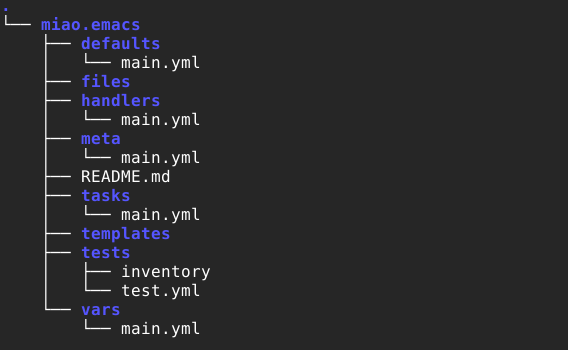
\includegraphics{/images/ansible-galaxy-init-structure.png}

\subsubsection{fill in information}\label{fill-in-information}

Let us fill in information to our project. There are several
\texttt{main.yml} files in different folders, and we will illustrate
their usages.

\begin{description}
\item[defaults and vars:]
These folders should hold variables key-value pairs for your playbook
scripts. We will leave them empty in this example.
\item[files:]
This folder is for files need to be copied to the target hosts. Data
files or configuration files can be specified if needed. We will leave
it empty too.
\item[templates:]
Similar missions to files/, templates is allocated for template files.
Keep empty for a simple Emacs installation.
\item[handlers:]
This is reserved for services running on target hosts. For example, to
restart a service under certain circumstance.
\end{description}

tasks:

\begin{quote}
This file is the actual script for all tasks. You can use the role you
built previously for Emacs installation here:

\begin{verbatim}
---
- name: install Emacs on Ubuntu 16.04
  become: yes
  package: name=emacs state=present
\end{verbatim}
\end{quote}

\begin{description}
\item[meta:]
Provide necessary metatdata for our Ansible Galaxy project for shipping:

\begin{verbatim}
---
galaxy_info:
  author: <you name>
  description: emacs installation on Ubuntu 16.04
  license:
    - MIT
  min_ansible_version: 2.0
  platforms:
    - name: Ubuntu
      versions:
        - xenial
  galaxy_tags:
    - development

dependencies: []
\end{verbatim}
\end{description}

\subsubsection{Test it out}\label{test-it-out}

You have your Ansible Galaxy role ready now. To test it as a user, go to
your HID directory and edit the other two files \texttt{inventory} and
\texttt{playbook.yml}, which are already generated for you in directory
\texttt{tests} by the script:

\begin{verbatim}
$ ansible-playbook -i ./hosts playbook.yml
\end{verbatim}

After running this playbook, you should have Emacs installed on
localhost.

\subsection{A Complete Ansible Galaxy
Project}\label{a-complete-ansible-galaxy-project}

We are going to use ansible-galaxy to setup a sample project. This
sample project will:

\begin{itemize}

\item
  use a cloud cluster with multiple VMs
\item
  deploy Apache Spark on this cluster
\item
  install a particular HPC application
\item
  prepare raw data for this cluster to process
\item
  run the experiment and collect results
\end{itemize}
\section{Ansible: Write a Playbooks for
MongoDB}\label{ansible-write-a-playbooks-for-mongodb}

Ansible Playbooks are automated scripts written in YAML data format.
Instead of using manual commands to setup multiple remote machines, you
can utilize Ansible Playbooks to configure your entire systems. YAML
syntax is easy to read and express the data structure of certain Ansible
functions. You simply write some tasks, for example, installing
software, configuring default settings, and starting the software, in a
Ansible Playbook. With a few examples in this tutorial, you will
understand how it works and how to write your own Playbooks.

\begin{description}
\item[There are also several examples of using Ansible
\href{http://docs.ansible.com/playbooks.html}{Playbooks} from the
official site. It covers]
from basic usage of Ansible Playbooks to advanced usage such as applying
patches and updates with different roles and groups.
\end{description}

\subsection{Tutorial: Writing Ansible
Playbook}\label{tutorial-writing-ansible-playbook}

In this tutorial, we are going to write a basic playbook of Ansible
software. Keep in mind that \texttt{Ansible} is a main program and
\texttt{playbook} is a template that you would like to use. You may have
several playbooks in your Ansible.

\subsubsection{First playbook for MongoDB
Installation}\label{first-playbook-for-mongodb-installation}

As a first example, we are going to write a playbook which installs
MongoDB server. It includes the following tasks:

\begin{itemize}

\item
  Import the public key used by the package management system
\item
  Create a list file for MongoDB
\item
  Reload local package database
\item
  Install the MongoDB packages
\item
  Start MongoDB
\end{itemize}

This tutorial is based on the manual installation of MongoDB from the
official site:
\url{http://docs.mongodb.org/manual/tutorial/install-mongodb-on-ubuntu/*}

We also assume that we install MongoDB on Ubuntu 15.10.

\subsubsection{Enabling Root SSH Access}\label{enabling-root-ssh-access}

Some setups of managed nodes may not allow you to log in as root. As
this may be problematic later, let us create a playbook to resolve this.
Create a \texttt{enable-root-access.yaml} file with the following
contents:

\begin{verbatim}
---
- hosts: ansible-test
  remote_user: ubuntu
  tasks:
    - name: Enable root login
      shell: sudo cp ~/.ssh/authorized_keys /root/.ssh/
\end{verbatim}

Explanation:

\begin{itemize}

\item
  \texttt{hosts} specifies the name of a group of machines in the
  inventory
\item
  \texttt{remote\_user} specifies the username on the managed nodes to
  log in as
\item
  \texttt{tasks} is a list of tasks to accomplish having a \texttt{name}
  (a description) and modules to execute. In this case we use the
  \texttt{shell} module.
\end{itemize}

We can run this playbook like so:

\begin{verbatim}
$ ansible-playbook -i inventory.txt -c ssh enable-root-access.yaml

PLAY [ansible-test] *********************************************************** 

GATHERING FACTS *************************************************************** 
ok: [10.23.2.105]
ok: [10.23.2.104]

TASK: [Enable root login] ***************************************************** 
changed: [10.23.2.104]
changed: [10.23.2.105]

PLAY RECAP ******************************************************************** 
10.23.2.104                : ok=2    changed=1    unreachable=0    failed=0   
10.23.2.105                : ok=2    changed=1    unreachable=0    failed=0
\end{verbatim}

\subsubsection{Hosts and Users}\label{hosts-and-users}

First step is choosing hosts to install MongoDB and a user account to
run commands (tasks). We start with the following lines in the example
filename of \texttt{mongodb.yaml}:

\begin{verbatim}
---
- hosts: ansible-test
  remote_user: root
  become: yes
\end{verbatim}

In a previous tutorial, we setup two machines with \texttt{ansible-test}
group name. This tutorial uses that two machines for MongoDB
installation. Also, we use \texttt{root} account to complete Ansible
tasks.

\begin{description}
\item[Indentation is important in YAML format. Do not ignore spaces
start]
with in each line.
\end{description}

\subsubsection{Tasks}\label{tasks}

A list of tasks contains commands or configurations to be executed on
remote machines in a sequential order. Each task comes with a
\texttt{name} and a \texttt{module} to run your command or
configuration. You provide a description of your task in \texttt{name}
section and choose a \texttt{module} for your task. There are several
modules that you can use, for example, \texttt{shell} module simply
executes a command without considering a return value. You may use
\texttt{apt} or \texttt{yum} module which is one of the packaging
modules to install software. You can find an entire list of modules
here: \url{http://docs.ansible.com/list_of_all_modules.html}

\subsubsection{\texorpdfstring{Module \texttt{apt\_key}: add repository
keys}{Module apt\_key: add repository keys}}\label{module-apt_key-add-repository-keys}

We need to import the MongoDB public GPG Key. This is going to be a
first task in our playbook.:

\begin{verbatim}
tasks:
  - name: Import the public key used by the package management system
    apt_key: keyserver=hkp://keyserver.ubuntu.com:80 id=7F0CEB10 state=present
\end{verbatim}

\subsubsection{\texorpdfstring{Module \texttt{apt\_repository}: add
repositories}{Module apt\_repository: add repositories}}\label{module-apt_repository-add-repositories}

Next add the MongoDB repository to apt:

\begin{verbatim}
- name: Add MongoDB repository
  apt_repository: repo='deb http://downloads-distro.mongodb.org/repo/ubuntu-upstart dist 10gen' state=present
\end{verbatim}

\subsubsection{\texorpdfstring{Module \texttt{apt}: install
packages}{Module apt: install packages}}\label{module-apt-install-packages}

We use \texttt{apt} module to install \texttt{mongodb-org} package.
\texttt{notify} action is added to start \texttt{mongod} after the
completion of this task. Use the \texttt{update\_cache=yes} option to
reload the local package database.:

\begin{verbatim}
- name: install mongodb
  apt: pkg=mongodb-org state=latest update_cache=yes
  notify:
  - start mongodb
\end{verbatim}

\subsubsection{\texorpdfstring{Module \texttt{service}: manage
services}{Module service: manage services}}\label{module-service-manage-services}

We use \texttt{handlers} here to start or restart services. It is
similar to \texttt{tasks} but will run only once.:

\begin{verbatim}
handlers:
  - name: start mongodb
    service: name=mongod state=started
\end{verbatim}

\subsubsection{The Full Playbook}\label{the-full-playbook}

Our first playbook looks like this:

\begin{verbatim}
---
- hosts: ansible-test
  remote_user: root
  become: yes
  tasks:
  - name: Import the public key used by the package management system
    apt_key: keyserver=hkp://keyserver.ubuntu.com:80 id=7F0CEB10 state=present
  - name: Add MongoDB repository
    apt_repository: repo='deb http://downloads-distro.mongodb.org/repo/ubuntu-upstart dist 10gen' state=present
  - name: install mongodb
    apt: pkg=mongodb-org state=latest update_cache=yes
    notify:
    - start mongodb
  handlers:
    - name: start mongodb
      service: name=mongod state=started
\end{verbatim}

\subsubsection{Running a Playbook}\label{running-a-playbook}

We use \texttt{ansible-playbook} command to run our playbook:

\begin{verbatim}
$ ansible-playbook -i inventory.txt -c ssh mongodb.yaml

PLAY [ansible-test] *********************************************************** 

GATHERING FACTS *************************************************************** 
ok: [10.23.2.104]
ok: [10.23.2.105]

TASK: [Import the public key used by the package management system] *********** 
changed: [10.23.2.104]
changed: [10.23.2.105]

TASK: [Add MongoDB repository] ************************************************ 
changed: [10.23.2.104]
changed: [10.23.2.105]

TASK: [install mongodb] ******************************************************* 
changed: [10.23.2.104]
changed: [10.23.2.105]

NOTIFIED: [start mongodb] ***************************************************** 
ok: [10.23.2.105]
ok: [10.23.2.104]

PLAY RECAP ******************************************************************** 
10.23.2.104                : ok=5    changed=3    unreachable=0    failed=0   
10.23.2.105                : ok=5    changed=3    unreachable=0    failed=0
\end{verbatim}

If you rerun the playbook, you should see that nothing changed:

\begin{verbatim}
$ ansible-playbook -i inventory.txt -c ssh mongodb.yaml 

PLAY [ansible-test] *********************************************************** 

GATHERING FACTS *************************************************************** 
ok: [10.23.2.105]
ok: [10.23.2.104]

TASK: [Import the public key used by the package management system] *********** 
ok: [10.23.2.104]
ok: [10.23.2.105]

TASK: [Add MongoDB repository] ************************************************ 
ok: [10.23.2.104]
ok: [10.23.2.105]

TASK: [install mongodb] ******************************************************* 
ok: [10.23.2.105]
ok: [10.23.2.104]

PLAY RECAP ******************************************************************** 
10.23.2.104                : ok=4    changed=0    unreachable=0    failed=0   
10.23.2.105                : ok=4    changed=0    unreachable=0    failed=0
\end{verbatim}

\subsubsection{Sanity Check: Test
MongoDB}\label{sanity-check-test-mongodb}

Let's try to run `mongo' to enter mongodb shell.:

\begin{verbatim}
$ ssh ubuntu@$IP
$ mongo
MongoDB shell version: 2.6.9
connecting to: test
Welcome to the MongoDB shell.
For interactive help, type "help".
For more comprehensive documentation, see
        http://docs.mongodb.org/
Questions? Try the support group
        http://groups.google.com/group/mongodb-user
> 
\end{verbatim}

\subsubsection{Terms}\label{terms}

\begin{itemize}

\item
  Module: Ansible library to run or manage services, packages, files or
  commands.
\item
  Handler: A task for notifier.
\item
  Task: Ansible job to run a command, check files, or update
  configurations.
\item
  Playbook: a list of tasks for Ansible nodes. YAML format used.
\item
  YAML: Human readable generic data serialization.
\end{itemize}

\subsubsection{Reference}\label{reference}

The main tutorial from Ansible is here:
\url{http://docs.ansible.com/playbooks_intro.html}

You can also find an index of the ansible modules here:
\url{http://docs.ansible.com/modules_by_category.html}
\section{Ansible Assignment}\label{ansible-assignment}

We have shown a couple of examples of using Ansible tools. Before you
apply it in you final project, we will practice it in this assignment.

\subsection{Requirements}\label{requirements}

\begin{itemize}

\item
  use the \texttt{galaxy} directory in the class assignment repository
\item
  set up the project structure similar to Ansible Galaxy example
\item
  install MongoDB from the package manager (apt in this class)
\item
  configure your MongoDB installation to start the service automatically
\item
  use default port and let it serve local client connections only
\end{itemize}

\section{Hadoop Virtual Cluster
Installation}\label{hadoop-virtual-cluster-installation}

\subsection{Cloudmesh Cluster
Installation}\label{cloudmesh-cluster-installation}

Before you start this lesson, you MUST finish cm\_install\_.

This lesson is created and test under the newest version of Cloudmesh
client. Update yours if not.

To manage virtual cluster on cloud, the command is \texttt{cm\ cluster}.
Try \texttt{cm\ cluster\ help} to see what other commands are and what
options they supported.

\subsubsection{Create Cluster}\label{create-cluster}

To create a virtual cluster on cloud, we must define an active cluster
specification with \texttt{cm\ cluster\ define} command. For example, we
define a cluster with 3 nodes:

\begin{verbatim}
$ cm cluster define --count 3
\end{verbatim}

\begin{description}
\item[All options will use the default setting if not specified during
cluster]
define. Try \texttt{cm\ cluster\ help} command to see what options
\texttt{cm\ cluster\ define} has and means, here is part of the usage
information: :
\end{description}

\$ cm cluster help usage: cluster create {[}-n NAME{]} {[}-c COUNT{]}
{[}-C CLOUD{]} {[}-u NAME{]} {[}-i IMAGE{]} {[}-f FLAVOR{]} {[}-k KEY{]}
{[}-s NAME{]} {[}-AI{]} Options: -A --no-activate Don't activate this
cluster -I --no-floating-ip Don't assign floating IPs -n NAME
--name=NAME Name of the cluster -c COUNT --count=COUNT Number of nodes
in the cluster -C NAME --cloud=NAME Name of the cloud -u NAME
--username=NAME Name of the image login user -i NAME --image=NAME Name
of the image -f NAME --flavor=NAME Name of the flavor -k NAME --key=NAME
Name of the key -s NAME --secgroup=NAME NAME of the security group -o
PATH --path=PATH Output to this path \ldots{}

\begin{description}
\item[Floating IP is a valuable and limited resource on cloud.]
\texttt{cm\ cluster\ define} will assign floating IP to every node
within the cluster by default. Cluster creation will fail if the
floating IPs run out on cloud. When you run into error like this, use
option \texttt{-I} or \texttt{-\/-no-floating-ip} to avoid assigning
floating IPs during cluster creation:
\end{description}

\$ cm cluster define --count 3 --no-floating-ip

\begin{quote}
Then manually assign floating IP to one of the nodes. Use this node as a
logging node or head node to log in to all the other nodes.
\end{quote}

We can have multiple specifications defined at the same time. Every time
a new cluster specification is defined, the counter of the default
cluster name will increment. Hence, the default cluster name will be
\texttt{cluster-001}, \texttt{cluster-002}, \texttt{cluster-003} and so
on. Use \texttt{cm\ cluster\ avail} to check all the available cluster
specifications:

\begin{verbatim}
$ cm cluster avail
  cluster-001
    count                         : 3
    image                         : CC-Ubuntu14.04
    key                           : xl41
    flavor                        : m1.small
    secgroup                      : default
    assignFloatingIP              : True
    cloud                         : chameleon
> cluster-002
    count                         : 3
    image                         : CC-Ubuntu14.04
    key                           : xl41
    flavor                        : m1.small
    secgroup                      : default
    assignFloatingIP              : False
    cloud                         : chameleon
\end{verbatim}

With \texttt{cm\ cluster\ use\ {[}NAME{]}}, we are able to switch
between different specifications with given cluster name:

\begin{verbatim}
$ cm cluster use cluster-001
$ cm cluster avail
> cluster-001
    count                         : 3
    image                         : CC-Ubuntu14.04
    key                           : xl41
    flavor                        : m1.small
    secgroup                      : default
    assignFloatingIP              : True
    cloud                         : chameleon
  cluster-002
    count                         : 3
    image                         : CC-Ubuntu14.04
    key                           : xl41
    flavor                        : m1.small
    secgroup                      : default
    assignFloatingIP              : False
    cloud                         : chameleon
\end{verbatim}

This will activate specification \texttt{cluster-001} which assigns
floating IP during creation rather than the latest one
\texttt{cluster-002}.

With our cluster specification ready, we create the cluster with command
\texttt{cm\ cluster\ allocate}. This will create a virtual cluster on
the cloud with the activated specification:

\begin{verbatim}
$ cm cluster allocate
\end{verbatim}

Each specification can have one active cluster, which means
\texttt{cm\ cluster\ \ \ allocate} does nothing if there is a
successfully active cluster.

\subsubsection{Check Created Cluster}\label{check-created-cluster}

With command \texttt{cm\ cluster\ list}, we can see the cluster with the
default name \texttt{cluster-001} we just created:

\begin{verbatim}
$ cm cluster list
cluster-001
\end{verbatim}

Using \texttt{cm\ cluster\ nodes\ {[}NAME{]}}, we can also see the nodes
of the cluster along with their assigned floating IPs of the cluster:

\begin{verbatim}
$ cm cluster nodes cluster-001
xl41-001 129.114.33.147
xl41-002 129.114.33.148
xl41-003 129.114.33.149
\end{verbatim}

If option \texttt{-\/-no-floating-ip} is included during definition, you
will see nodes without floating IP:

\begin{verbatim}
$ cm cluster nodes cluster-002
xl41-004 None
xl41-005 None
xl41-006 None
\end{verbatim}

To log in one of them, use command
\texttt{cm\ vm\ assign\ IP\ {[}NAME{]}} to assign a floating IP to one
of them:

\begin{verbatim}
$ cm vm ip assign xl41-006
$ cm cluster nodes cluster-002
xl41-004 None
xl41-005 None
xl41-006 129.114.33.150
\end{verbatim}

Then you can log in this node as a head node of your cluster by
\texttt{cm\ vm\ ssh\ {[}NAME{]}}:

\begin{verbatim}
$ cm vm ssh xl41-006
cc@xl41-006 $
\end{verbatim}

\subsubsection{Delete Cluster}\label{delete-cluster}

Using \texttt{cm\ cluster\ delete\ {[}NAME{]}}, we are able to delete
the cluster we created:

\begin{verbatim}
$ cm cluster delete cluster-001
\end{verbatim}

\begin{description}
\item[Option \texttt{-\/-all} can delete all the clusters created, so be
careful:]
:
\end{description}

\$ cm cluster delete --all

Then we need to undefine our cluster specification with command
\texttt{cm\ cluster\ undefine\ {[}NAME{]}}:

\begin{verbatim}
$ cm cluster undefine cluster-001
\end{verbatim}

Option \texttt{-\/-all} can delete all the cluster specifications:

\begin{verbatim}
$ cm cluster undefine --all
\end{verbatim}

\subsection{Hadoop Cluster
Installation}\label{hadoop-cluster-installation}

This section is built upon the previous one. Please finish the previous
one before start this one.

\subsubsection{Create Hadoop Cluster}\label{create-hadoop-cluster}

To create a Hadoop cluster, we need to first define a cluster with
\texttt{cm\ cluster\ define} command:

\begin{verbatim}
$ cm cluster define --count 3
\end{verbatim}

\begin{description}
\item[To deploy a Hadoop cluster, we only support image
\texttt{CC-Ubuntu14.04}]
on Chameleon. DO NOT use \texttt{CC-Ubuntu16.04} or any other images.
You will need to specify it if it's not the default image:
\end{description}

\$ cm cluster define --count 3 --image CC-Ubuntu14.04

Then we define the Hadoop cluster upon the cluster we defined using
\texttt{cm\ hadoop\ define} command:

\begin{verbatim}
$ cm hadoop define
\end{verbatim}

Same as \texttt{cm\ cluster\ define}, you can define multiple
specifications for the Hadoop cluster and check them with
\texttt{cm\ hadoop\ avail}:

\begin{verbatim}
$ cm hadoop avail
> stack-001
  local_path                    : /Users/tony/.cloudmesh/stacks/stack-001
  addons                        : []
\end{verbatim}

We can use \texttt{cm\ hadoop\ use\ {[}NAME{]}} to activate the
specification with the given name:

\begin{verbatim}
$ cm hadoop use stack-001
\end{verbatim}

May not be available for current version of Cloudmesh Client.

Before deploy, we need to use \texttt{cm\ hadoop\ sync} to checkout /
synchronize the Big Data Stack from Github.com:

\begin{verbatim}
$ cm hadoop sync
\end{verbatim}

\begin{description}
\item[To avoid errors, make sure you are able to connect to Github.com
using SSH:]
\url{https://help.github.com/articles/connecting-to-github-with-ssh/}.
\end{description}

Finally, we are ready to deploy our Hadoop cluster:

\begin{verbatim}
$ cm hadoop deploy
\end{verbatim}

This process could take up to 10 minutes based on your network.

To check Hadoop is working or not. Use \texttt{cm\ vm\ ssh} to log into
the \texttt{Namenode} of the Hadoop cluster. It's usually the first node
of the cluster:

\begin{verbatim}
$ cm vm ssh node-001
cc@hostname$
\end{verbatim}

Switch to user \texttt{hadoop} and check HDFS is set up or not:

\begin{verbatim}
cc@hostname$ sudo su - hadoop
hadoop@hostname$ hdfs dfs -ls /
Found 1 items
drwxrwx---   - hadoop hadoop,hadoopadmin          0 2017-02-15 17:26 /tmp
\end{verbatim}

Now the Hadoop cluster is properly installed and configured.

\subsubsection{Delete Hadoop Cluster}\label{delete-hadoop-cluster}

To delete the Hadoop cluster we created, use command
\texttt{cm\ cluster\ delete\ {[}NAME{]}} to delete the cluster with
given name:

\begin{verbatim}
$ cm cluster delete cluster-001
\end{verbatim}

Then undefine the Hadoop specification and the cluster specification:

\begin{verbatim}
$ cm hadoop undefine stack-001
$ cm cluster undefine cluster-001
\end{verbatim}

May not be available for current version of Cloudmesh Client.

\subsection{Advanced Topics with
Hadoop}\label{advanced-topics-with-hadoop}

\subsubsection{Hadoop Virtual Cluster with Spark and/or
Pig}\label{hadoop-virtual-cluster-with-spark-andor-pig}

To install Spark and/or Pig with Hadoop cluster, we first use command
\texttt{cm\ hadoop\ define} but with \texttt{ADDON} to define the
cluster specification.

For example, we create a 3-node Spark cluster with Pig. To do that, all
we need is to specify \texttt{spark} as an \texttt{ADDON} during Hadoop
definition:

\begin{verbatim}
$ cm cluster define --count 3
$ cm hadoop define spark pig
\end{verbatim}

Using \texttt{cm\ hadoop\ addons}, we are able to check the current
supported addon:

\begin{verbatim}
$ cm hadoop addons
\end{verbatim}

With \texttt{cm\ hadoop\ avail}, we can see the detail of the
specification for the Hadoop cluster:

\begin{verbatim}
$ cm hadoop avail
> stack-001
  local_path                    : /Users/tony/.cloudmesh/stacks/stack-001
  addons                        : [u'spark', u'pig']
\end{verbatim}

Then we use \texttt{cm\ hadoop\ sync} and \texttt{cm\ hadoop\ deploy} to
deploy our Spark cluster:

\begin{verbatim}
$ cm hadoop sync
$ cm hadoop deploy
\end{verbatim}

This process will take 15 minutes or longer.

Before we proceed to the next step, there is one more thing we need to,
which is to make sure we are able to ssh from every node to others
without password. To achieve that, we need to execute
\texttt{cm\ cluster\ cross\_ssh}:

\begin{verbatim}
$ cm cluster cross_ssh
\end{verbatim}

\subsubsection{Word Count Example on
Spark}\label{word-count-example-on-spark}

Now with the cluster ready, let's run a simple Spark job, Word Count, on
one of William Shakespear's work. Use \texttt{cm\ vm\ ssh} to log into
the \texttt{Namenode} of the Spark cluster. It should be the first node
of the cluster:

\begin{verbatim}
$ cm vm ssh node-001
cc@hostname$
\end{verbatim}

Switch to user \texttt{hadoop} and check HDFS is set up or not:

\begin{verbatim}
cc@hostname$ sudo su - hadoop
hadoop@hostname$
\end{verbatim}

Download the input file from the Internet:

\begin{verbatim}
wget --no-check-certificate -O inputfile.txt \
https://ocw.mit.edu/ans7870/6/6.006/s08/lecturenotes/files/t8.shakespeare.txt
\end{verbatim}

You can also use any other text file you preferred. Create a new
directory \texttt{wordcount} within HDFS to store the input and output:

\begin{verbatim}
$ hdfs dfs -mkdir /wordcount
\end{verbatim}

Store the input text file into the directory:

\begin{verbatim}
$ hdfs dfs -put inputfile.txt /wordcount/inputfile.txt
\end{verbatim}

Save the following code as \texttt{wordcount.py} on the local file
system on Namenode:

\begin{verbatim}
import sys

from pyspark import SparkContext, SparkConf

if __name__ == "__main__":

  # tak two arguments, input and output
  if len(sys.argv) != 3:
    print("Usage: wordcount <input> <output>")
    exit(-1)

  # create Spark context with Spark configuration
  conf = SparkConf().setAppName("Spark Count")
  sc = SparkContext(conf=conf)

  # read in text file
  text_file = sc.textFile(sys.argv[1])

  # split each line into words
  # count the occurrence of each word
  # sort the output based on word
  counts = text_file.flatMap(lambda line: line.split(" ")) \
           .map(lambda word: (word, 1)) \
           .reduceByKey(lambda a, b: a + b) \
           .sortByKey()

  # save the result in the output text file
  counts.saveAsTextFile(sys.argv[2])
\end{verbatim}

Next submit the job to Yarn and run in distribute:

\begin{verbatim}
$ spark-submit --master yarn --deploy-mode client --executor-memory 1g \
--name wordcount --conf "spark.app.id=wordcount" wordcount.py \
hdfs://192.168.0.236:8020/wordcount/inputfile.txt \
hdfs://192.168.0.236:8020/wordcount/output
\end{verbatim}

Finally, take a look at the result in the output directory:

\begin{verbatim}
$ hdfs dfs -ls /wordcount/outputfile/
Found 3 items
-rw-r--r--   1 hadoop hadoop,hadoopadmin          0 2017-03-07 21:28 /wordcount/output/_SUCCESS
-rw-r--r--   1 hadoop hadoop,hadoopadmin     483182 2017-03-07 21:28 /wordcount/output/part-00000
-rw-r--r--   1 hadoop hadoop,hadoopadmin     639649 2017-03-07 21:28 /wordcount/output/part-00001
$ hdfs dfs -cat /wordcount/output/part-00000 | less
(u'', 517065)
(u'"', 241)
(u'"\'Tis', 1)
(u'"A', 4)
(u'"AS-IS".', 1)
(u'"Air,"', 1)
(u'"Alas,', 1)
(u'"Amen"', 2)
(u'"Amen"?', 1)
(u'"Amen,"', 1)
...
\end{verbatim}

\section{Box}\label{box}

what is box

Link:

\begin{itemize}

\item
  \url{http://opensource.box.com/box-python-sdk/tutorials/intro.html}
\item
  \url{https://github.com/box/box-python-sdk/tree/1.5/demo}
\end{itemize}

Install:

\begin{verbatim}
pip install boxsdk
\end{verbatim}

app.cfg:

\begin{verbatim}
* A Box client ID for a Box application
* The corresponding Box client secret
* A valid developer token for that application
\end{verbatim}

code:

\begin{verbatim}
# Import two classes from the boxsdk module - Client and OAuth2
from boxsdk import Client, OAuth2

# Define client ID, client secret, and developer token.
CLIENT_ID = None
CLIENT_SECRET = None
ACCESS_TOKEN = None

# Read app info from text file
with open('app.cfg', 'r') as app_cfg:
  CLIENT_ID = app_cfg.readline()
  CLIENT_SECRET = app_cfg.readline()
  ACCESS_TOKEN = app_cfg.readline()

# Create OAuth2 object. It's already authenticated, thanks to the developer token.
oauth2 = OAuth2(CLIENT_ID, CLIENT_SECRET, access_token=ACCESS_TOKEN)

# Create the authenticated client
client = Client(oauth2, LoggingNetwork())

# Get information about the logged in user (that's whoever owns the developer token)
my = client.user(user_id='me').get()
print (my.name)
print (my.login)
print (my.avatar_url)

root_folder = client.folder('0')
root_folder_with_info = root_folder.get()

print (root_folder_with_info)
\end{verbatim}

Questions

\begin{itemize}

\item
  how to list all file sin dir
\item
  how to recursively iterate
\item
  how to download each file when we iterate
\end{itemize}

\subsection{boxpython}\label{boxpython}

* \url{https://github.com/wesleyfr/boxpython}

\begin{quote}
from boxpython import BoxAuthenticateFlow, BoxSession, BoxError
\end{quote}

\textgreater{}\textgreater{}\textgreater{}
\textgreater{}\textgreater{}\textgreater{} flow =
BoxAuthenticateFlow(`\textless{}client\_id\textgreater{}',
`\textless{}client\_secret\textgreater{}')
\textgreater{}\textgreater{}\textgreater{}
flow.get\_authorization\_url()
`\url{https://www.box.com/api/oauth2/authorize?response_type=code\&client_id}=\textless{}client\_id\textgreater{}\&state=authenticated'
\textgreater{}\textgreater{}\textgreater{}

access\_token, refresh\_token =
flow.get\_access\_tokens(`\textless{}auth\_code\textgreater{}')

def tokens\_changed(refresh\_token, access\_token): \ldots{}
save\_to\_file(refresh\_token, access\_token) \ldots{}
\textgreater{}\textgreater{}\textgreater{} box =
BoxSession(`\textless{}client\_id\textgreater{}',
`\textless{}client\_secret\textgreater{}', refresh\_token,
access\_token, tokens\_changed)

box.get\_folder\_info(0)

box.download\_file(11006194629, `/tmp/test\_dl.txt')

\subsection{Pybox}\label{pybox}

\url{https://github.com/hzheng/pybox}

\section{Anaconda}\label{anaconda}

\begin{description}
\item[We do not recommend that you use anaconda as it may]
interfere with your default python interpreters and setup.
\end{description}

\begin{description}
\item[This section about anaconda is experimental and has not]
been tested.
\end{description}

You can add anaconda to your pyenv with the following commands:

\begin{verbatim}
pyenv install anaconda2-4.3.1
pyenv install anaconda3-4.3.1
\end{verbatim}

Here we install both the version 2 and version 3 python environments
from anavconda. Please be aware that the install may tacke several
minutes. Make sure to install the latest release which you can find out
if you leave of the version after the 2 or 3.

When executing:

\begin{verbatim}
pyenv versions
\end{verbatim}

you will see after the install completed the anaconda versiosn
installed:

\begin{verbatim}
pyenv versions
system
2.7.13
2.7.13/envs/ENV2
3.6.1
3.6.1/envs/ENV3
* ENV2 (set by PYENV_VERSION environment variable)
ENV3
anaconda2-4.3.1
anaconda3-4.3.1
\end{verbatim}

Let us now create virtualenv for anaconda:

\begin{verbatim}
$ pyenv virtualenv anaconda2-4.3.1 ANA2
$ pyenv virtualenv anaconda3-4.3.1 ANA3
\end{verbatim}

\section{Excersise}\label{excersise}

\begin{description}
\item[Econda.1:]
Write installation instructions for an operating system of your choice
and add to this documentation.
\item[Econda.2:]
Replicate the steps above, so you can type in ENV2 and ENV3 in your
terminals to switch between python 2 and 3.
\end{description}

\section{Python for Big Data}\label{python-for-big-data}

\subsection{An Example with Pandas, NumPy and
Matplotlib}\label{an-example-with-pandas-numpy-and-matplotlib}

In this example, we will download some traffic citation data for the
city of Bloomington, IN, load it into Python and generate a histogram.
In doing so, you will be exposed to important Python libraries for
working with big data such as \href{www.numpy.org}{numpy},
\href{pandas.pydata.org}{pandas} and \href{matplotlib.org}{matplotlib}.

\subsubsection{Set Up Directories and Get Test
Data}\label{set-up-directories-and-get-test-data}

Data.gov is a government portal for open data and the
\href{https://catalog.data.gov/dataset?organization_type=City+Government\&organization=city-of-bloomington\&_organization_limit=0}{city
of Bloomington, Indiana makes available a number of datasets there}.

We will use traffic citations data for 2016.

To start, let's create a separate directory for this project and
download the CSV data:

\begin{verbatim}
$ cd ~/projects/i524
$ mkdir btown-citations
$ cd btown-citations
$ wget https://data.bloomington.in.gov/dataset/c543f0c1-1e37-46ce-a0ba-e0a949bd248a/resource/24841976-fd35-4483-a2b4-573bd1e77cfb/download/2016-first-quarter-citations.csv
\end{verbatim}

Depending on your directory organization, the above might be slightly
different for you.

If you go to the link to data.gov for Bloomington above, you will see
that the citations data is organized per quarter, so there are a total
of four files. Above, we downloaded the data for the first quarter. Go
ahead and download the remaining three files with \texttt{wget}.

In this example, we will use three modules, \texttt{numpy},
\texttt{pandas} and \texttt{matplotlib}. If you set up
\texttt{virtualenv} as described in the
Python tutorial \textless{}python\_intro\textgreater{}, the first two of
these are already installed for you. To install \texttt{matplotlib},
make sure you've activated your \texttt{virtualenv} and use
\texttt{pip}:

\begin{verbatim}
$ source ~/ENV/bin/activate
$ pip install matplotlib
\end{verbatim}

If you are using a different distribution of Python, you will need to
make sure that all three of these modules are installed.

\subsubsection{Load Data in Pandas}\label{load-data-in-pandas}

From the same directory where you saved the citations data, let's start
the Python interpreter and load the citations data for Q1 2016

\begin{verbatim}
$ python
>>> from __future__ import division, print_function
>>> import numpy as np
>>> import pandas as pd
>>> import matplotlib.pyplot as plt
>>> data = pd.read_csv('2016-first-quarter-citations.csv')
\end{verbatim}

If the first \texttt{import} statement seems confusing, take a look at
the Python tutorial \textless{}python\_intro\textgreater{}. The next
three \texttt{import} statements load each of the modules we will use in
this example. The final line uses Pandas' \texttt{read\_csv} function to
load the data into a Pandas \texttt{DataFrame} data structure.

\subsubsection{Working with DataFrames}\label{working-with-dataframes}

You can verify that you are working with a \texttt{DataFrame} and use
some of its methods to take a look at the structure of the data as
follows:

\begin{verbatim}
>>> type(data)
<class 'pandas.core.frame.DataFrame'>
>>> data.index
Int64Index([  0,   1,   2,   3,   4,   5,   6,   7,   8,   9,
...
197, 198, 199, 200, 201, 202, 203, 204, 205, 206],
dtype='int64', length=200)
>>> data.columns
Index([u'Citation Number', u'Date Issued', u'Time Issued', u'Location ',
u'District', u'Cited Person Age', u'Cited Person Sex',
u'Cited Person Race', u'Offense Code', u'Offense Description',
u'Officer Age', u'Officer Sex', u'Officer Race'],
dtype='object')
>>> data.dtypes
Citation Number                object
Date Issued                    object
Time Issued                    object
Location                       object
District                       object
Cited Person Age              float64
Cited Person Sex               object
Cited Person Race              object
Offense Code                   object
Offense Description            object
Officer Age                   float64
Officer Sex                    object
Officer Race                   object
dtype: object
>>> data.shape
(200, 15)
\end{verbatim}

As you can see from the \texttt{columns} field, when the CSV file was
read, the header line was used to populate the name of the columns in
the \texttt{DataFrame}. In addition, you will notice that
\texttt{read\_csv} correctly inferred the data type of some columns like
\emph{Age}, but not of others like \emph{Date Issued} and \emph{Time
Issued}. \texttt{read\_csv} is a very customizable function and in
general, you can correct issues like this using the \texttt{dtype} and
\texttt{converters} parameters. In this specific case, it makes more
sense to combine the \emph{Date Issued} and \emph{Time Issued} columns
into a new column containing a time stamp. We will see how to do this
shortly.

You can also look at the data itself with the \texttt{DataFrame}'s
\texttt{head()} and \texttt{tail()} methods:

\begin{verbatim}
>>> data.head()
<Output omitted for brevity>
>>> data.tail()
<Output omitted for brevity>
\end{verbatim}

In addition to letting you examine your data easily, \texttt{DataFrame}s
have methods that help you deal with missing values:

\begin{verbatim}
>>> data = data.dropna(how='any')
>>> data.shape
\end{verbatim}

Adding columns to the data is also easy. Here, we add two columns.
First, a
\href{https://docs.python.org/2/library/datetime.html}{datetime} column
that is a combination of the \texttt{Date\ Issued} and
\texttt{Time\ Issued} columns originally in the data. Second, a column
identifying what day of the week each citation was given. To understand
this example better, take a look at the Python docs for the
\texttt{strptime} and \texttt{strftime} functions in the
\texttt{datetime} module linked above.

\begin{verbatim}
>>> from datetime import datetime
>>> data['DateTime Issued'] = data.apply(
...  lambda row: datetime.strptime(row['Date Issued'] + ':' + row['Time Issued'], '%m/%d/%y:%I:%M %p'), axis=1
... )
>>> data.columns
>>> data['Day of Week Issued'] = data.apply(
...  lambda row: datetime.strftime(row['DateTime Issued'], '%A'), axis=1
... )
\end{verbatim}

\subsubsection{Plotting with Matplotlib and
NumPy}\label{plotting-with-matplotlib-and-numpy}

Let's say we want to see how many citations were given each day of the
week. We gather the data first:

\begin{verbatim}
>>> days = ['Monday', 'Tuesday', 'Wednesday', 'Thursday', 'Friday', 'Saturday', 'Sunday']
>>> dow_data = [days.index(dow) for dow in data['Day of Week Issued']]
>>> dow_data
<Output omitted for brevity>
\end{verbatim}

Then we use \texttt{matplotlib} to plot it:

\begin{verbatim}
>>> fig = plt.figure()
>>> ax = fig.add_subplot(1, 1, 1)
>>> plt.hist(dow_data, bins=len(days))
>>> plt.xticks(range(len(days)), days)
>>> plt.show()
\end{verbatim}

You should see something like this on your screen:

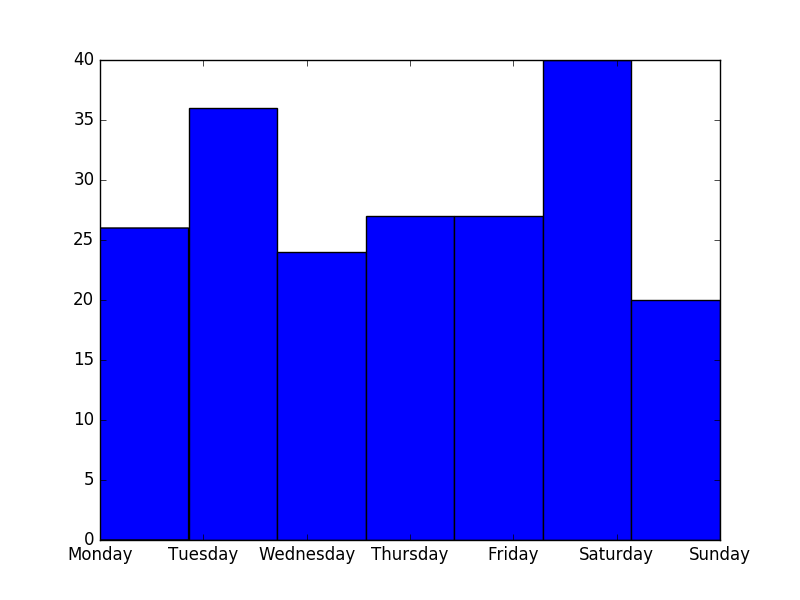
\includegraphics[width=4.16667in]{dow.png}

\subsubsection{\texorpdfstring{More \emph{DataFrame} Manipulation and
Plotting}{More DataFrame Manipulation and Plotting}}\label{more-dataframe-manipulation-and-plotting}

\texttt{DataFrame}s and \texttt{numpy} give us other ways to manipulate
data. For example, we can plot a histogram of the ages of violators like
this:

\begin{verbatim}
>>> ages = data['Cited Person Age'].astype(int)
>>> fig = plt.figure()
>>> ax = fig.add_subplot(1, 1, 1)
>>> plt.hist(ages, bins=np.max(ages) - np.min(ages))
>>> plt.show()
\end{verbatim}

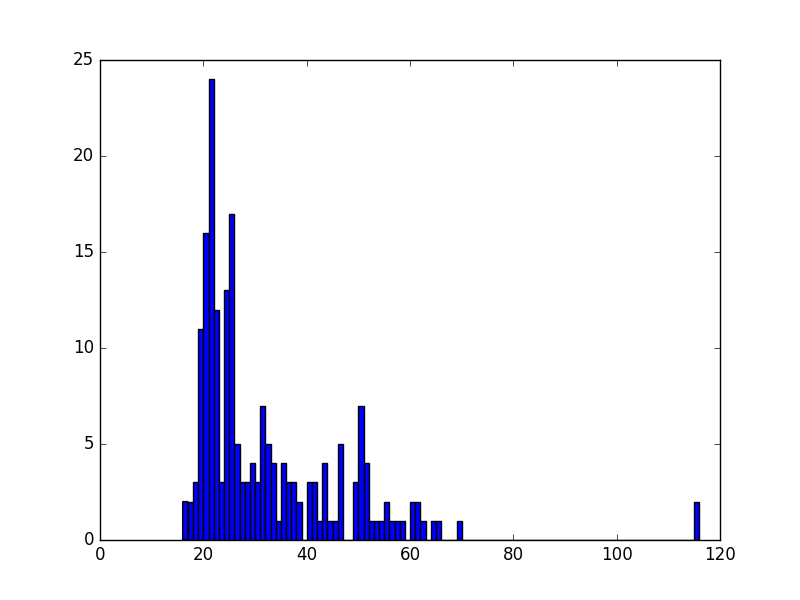
\includegraphics[width=4.16667in]{ages.png}

Surprisingly, we see some 116 year-old violators! This is probably an
error in the data, so we can remove these data points easily and plot
the histogram again:

\begin{verbatim}
>>> ages = ages[ages < 100]
>>> fig = plt.figure()
>>> ax = fig.add_subplot(1, 1, 1)
>>> plt.hist(ages, bins=np.max(ages) - np.min(ages))
>>> plt.show()
\end{verbatim}

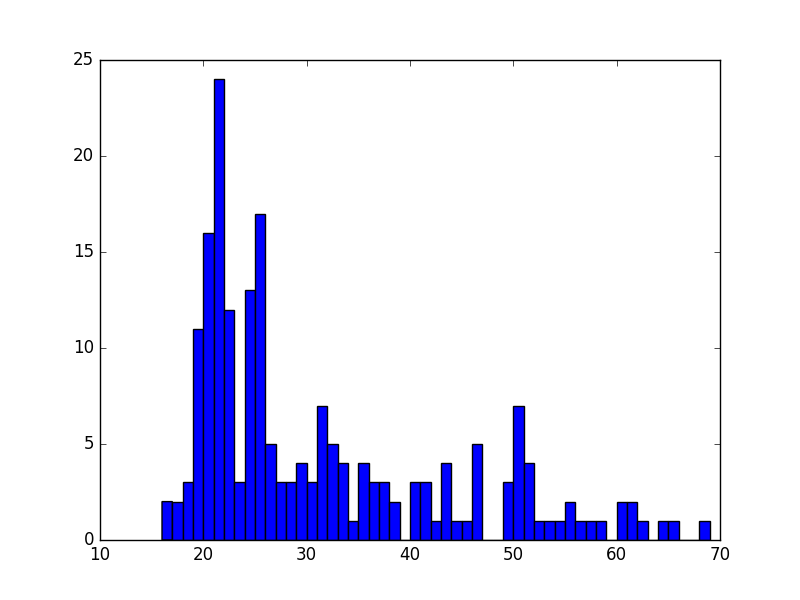
\includegraphics[width=4.16667in]{ages-filtered.png}

\subsubsection{Saving Plots to PDF}\label{saving-plots-to-pdf}

Oftentimes, you will want to save your \texttt{matplotlib} graph as a
PDF or an SVG file instead of just viewing it on your screen. For both,
we need to create a \texttt{figure} and plot the histogram as before:

\begin{verbatim}
>>> fig = plt.figure()
>>> ax = fig.add_subplot(1, 1, 1)
>>> plt.hist(ages, bins=np.max(ages) - np.min(ages))
\end{verbatim}

Then, instead of calling \texttt{plt.show()} we can invoke
\texttt{plt.savefig()} to save as SVG:

\begin{verbatim}
>>> plt.savefig('hist.svg')
\end{verbatim}

If we want to save the figure as PDF instead, we need to use the
\texttt{PdfPages} module together with \texttt{savefig()}:

\begin{verbatim}
>>> import matplotlib.patches as mpatches
>>> from matplotlib.backends.backend_pdf import PdfPages   
>>> pp = PdfPages('hist.pdf')
>>> fig.savefig(pp, format='pdf')
>>> pp.close()
\end{verbatim}

\subsubsection{Next Steps and Exercises}\label{next-steps-and-exercises}

There is a lot more to working with \texttt{pandas}, \texttt{numpy} and
\texttt{matplotlib} than we can show you here, but hopefully this
example has piqued your curiosity.

Don't worry if you don't understand everything in this example. For a
more detailed explanation on these modules and the examples we did,
please take a look at the tutorials below. The \texttt{numpy} and
\texttt{pandas} tutorials are mandatory if you want to be able to use
these modules, and the \texttt{matplotlib} gallery has many useful code
examples.

\subsection{Summary of Useful
Libraries}\label{summary-of-useful-libraries}

\subsubsection{Numpy}\label{numpy}

\begin{itemize}
\tightlist
\item
  \url{http://www.numpy.org/}
\end{itemize}

According to the Numpy Web page "NumPy is a package for scientific
computing with Python. It contains a powerful N-dimensional array
object, sophisticated (broadcasting) functions, tools for integrating
C/C++ and Fortran code, useful linear algebra, Fourier transform, and
random number capabilities

Tutorial:
\url{https://docs.scipy.org/doc/numpy-dev/user/quickstart.html}

\subsubsection{MatplotLib}\label{matplotlib}

\begin{itemize}
\tightlist
\item
  \url{http://matplotlib.org/}
\end{itemize}

According the the Matplotlib Web page, ``matplotlib is a python 2D
plotting library which produces publication quality figures in a variety
of hardcopy formats and interactive environments across platforms.
matplotlib can be used in python scripts, the python and ipython shell
(ala MATLAB®* or Mathematica®†), web application servers, and six
graphical user interface toolkits.''

Matplotlib Gallery: \url{http://matplotlib.org/gallery.html}

\subsubsection{Pandas}\label{pandas}

\begin{itemize}
\tightlist
\item
  \url{http://pandas.pydata.org/}
\end{itemize}

According to the Pandas Web page, ``Pandas is a library library
providing high-performance, easy-to-use data structures and data
analysis tools for the Python programming language.''

In addition to access to charts via matplotlib it has elementary
functionality for conduction data analysis. Pandas may be very suitable
for your projects.

Tutorial: \url{http://pandas.pydata.org/pandas-docs/stable/10min.html}

Pandas Cheat Sheet:
\url{https://github.com/pandas-dev/pandas/blob/master/doc/cheatsheet/Pandas_Cheat_Sheet.pdf}

\subsection{Other Useful Libraries}\label{other-useful-libraries}

\subsubsection{Scipy}\label{scipy}

\begin{itemize}
\tightlist
\item
  \url{https://www.scipy.org/}
\end{itemize}

According to the SciPy Web page, ``SciPy (pronounced ``Sigh Pie'') is a
Python-based ecosystem of open-source software for mathematics, science,
and engineering. In particular, these are some of the core packages:

\begin{itemize}
\tightlist
\item
  NumPy
\item
  IPython
\item
  Pandas
\item
  Matplotlib
\item
  Sympy
\item
  SciPy library
\end{itemize}

It is thus an agglomeration of useful pacakes and will prbably sufice
for your projects in case you use Python.

\subsubsection{ggplot}\label{ggplot}

\begin{itemize}
\tightlist
\item
  \url{http://ggplot.yhathq.com/}
\end{itemize}

According to the ggplot python Web page ggplot is a plotting system for
Python based on R's ggplot2. It allows to quickly generate some plots
quickly with little effort. Often it may be easier to use than
matplotlib directly.

\subsubsection{seaborn}\label{seaborn}

\url{http://www.data-analysis-in-python.org/t_seaborn.html}

The good library for plotting is called seaborn which is build on top of
matplotlib. It provides high level templates for common statistical
plots.

\begin{itemize}
\tightlist
\item
  Gallery:
  \url{http://stanford.edu/~mwaskom/software/seaborn/examples/index.html}
\item
  Original Tutorial:
  \url{http://stanford.edu/~mwaskom/software/seaborn/tutorial.html}
\item
  Additional Tutorial:
  \url{https://stanford.edu/~mwaskom/software/seaborn/tutorial/distributions.html}
\end{itemize}

\subsubsection{Bokeh}\label{bokeh}

Bokeh is an interactive visualization library with focus on web browsers
for display. Its goal is to provide a similar experience as D3.js

\begin{itemize}
\tightlist
\item
  URL: \url{http://bokeh.pydata.org/}
\item
  Gallery: \url{http://bokeh.pydata.org/en/latest/docs/gallery.html}
\end{itemize}

\subsubsection{pygal}\label{pygal}

Pygal is a simple API to produce graphs that can be easily embedded into
your Web pages. It contains annotations when you hover over data points.
It also allows to present the data in a table.

\begin{itemize}
\tightlist
\item
  URL: \url{http://pygal.org/}
\end{itemize}

\subsubsection{Network and Graphs}\label{network-and-graphs}

\begin{itemize}
\tightlist
\item
  igraph: \url{http://www.pythonforsocialscientists.org/t_igraph.html}
\item
  networkx: \url{https://networkx.github.io/}
\end{itemize}

\subsubsection{REST}\label{rest}

\begin{itemize}
\tightlist
\item
  django REST FRamework \url{http://www.django-rest-framework.org/}
\item
  flask
  \url{https://blog.miguelgrinberg.com/post/designing-a-restful-api-with-python-and-flask}
\item
  requests
  \url{https://realpython.com/blog/python/api-integration-in-python/}
\item
  urllib2
  \url{http://rest.elkstein.org/2008/02/using-rest-in-python.html} (not
  recommended)
\item
  web
  \url{http://www.dreamsyssoft.com/python-scripting-tutorial/create-simple-rest-web-service-with-python.php}
  (not recommended)
\item
  bottle \url{http://bottlepy.org/docs/dev/index.html}
\item
  falcon \url{https://falconframework.org/}
\item
  eve \url{http://python-eve.org/}
\item
  \url{https://code.tutsplus.com/tutorials/building-rest-apis-using-eve--cms-22961}
\end{itemize}

\subsection{Other Examples}\label{other-examples}

\begin{itemize}
\tightlist
\item
  Fingerprint Analysis \textless{}python\_lesson1\textgreater{}
\end{itemize}

\section{REST with Eve}\label{rest-with-eve}

\subsection{Overview of REST}\label{overview-of-rest}

REST stands for REpresentational State Transfer. REST is an architecture
style for designing networked applications. It is based on stateless,
client-server, cacheable communications protocol. Although not based on
http, in most cases, the HTTP protocol is used. In contrast to what some
others write or say, REST is not a \emph{standard}.

RESTful applications use HTTP requests to:

\begin{itemize}
\tightlist
\item
  post data: while creating and/or updating it,
\item
  read data: while making queries, and
\item
  delete data.
\end{itemize}

Hence REST uses HTTP for the four CRUD operations:

\begin{itemize}
\tightlist
\item
  Create
\item
  Read
\item
  Update
\item
  Delete
\end{itemize}

As part of the HTTP protocol we have methods such as GET, PUT, POST, and
DELETE. These methods can than be used to implement a REST service. As
REST introduces collections and items we need to implement the CRUD
functions for them. The semantics is explained in the Table
illustrationg how to implement them with HTTP methods.

Source:
\url{https://en.wikipedia.org/wiki/Representational_state_transfer}

\subsection{REST and eve}\label{rest-and-eve}

Now that we have outlined the basic functionality that we need, we lke
to introduce you to Eve that makes this process rather trivial. We will
provide you with an implementation example that showcases that we can
create REST services without writing a single line of code. The code for
this is located at \url{https://github.com/cloudmesh/rest}

This code will have a master branch but will also have a dev branch in
which we will add gradually more objects. Objects in the dev branch will
include:

\begin{itemize}
\tightlist
\item
  virtual directories
\item
  virtual clusters
\item
  job sequences
\item
  inventories
\end{itemize}

;You may want to check our active development work in the dev branch.
However for the purpose of this class the master branch will be
sufficient.

\subsubsection{Installation}\label{installation}

First we havt to install mongodb. The instalation will depend on your
operating system. For the use of the rest service it is not important to
integrate mongodb into the system upon reboot, which is focus of many
online documents. However, for us it is better if we can start and stop
the services explicitly for now.

On ubuntu, you need to do the following steps:

\begin{verbatim}
TO BE CONTRIBUTED BY THE STUDENTS OF THE CLASS as homework
\end{verbatim}

On windows 10, you need to do the following steps:

\begin{verbatim}
TO BE CONTRIBUTED BY THE STUDENTS OF THE CLASS as homework, if you
elect Windows 10. YOu could be using the online documentation
provided by starting it on Windows, or rinning it in a docker container.
\end{verbatim}

On OSX you can use homebrew and install it with:

\begin{verbatim}
brew update
brew install mongodb
\end{verbatim}

\begin{description}
\item[In future we may want to add ssl authentication in which case you
may]
need to install it as follows:
\end{description}

brew install mongodb --with-openssl

\subsubsection{Starting the service}\label{starting-the-service}

We have provided a convenient Makefile that currently only works for
OSX. It will be easy for you to adapt it to Linux. Certainly you can
look at the targes in the makefile and replicate them one by one.
Improtaht targest are deploy and test.

When using the makefile you can start the services with:

\begin{verbatim}
make deploy
\end{verbatim}

IT will start two terminals. IN one you will see the mongo service, in
the other you will see the eve service. The eve service will take a file
called sample.settings.py that is base on sample.json for the start of
the eve service. The mongo servide is configured in suc a wahy that it
only accepts incimming connections from the local host which will be
suffiicent fpr our case. The mongo data is written into the
\$USER/.cloudmesh directory, so make sure it exists.

To test the services you can say:

\begin{verbatim}
make test
\end{verbatim}

YOu will se a number of json text been written to the screen.

\subsection{Creating your own objects}\label{creating-your-own-objects}

The example demonstrated how easy it is to create a mongodb and an eve
rest service. Now lets use this example to creat your own. FOr this we
have modified a tool called evegenie to install it onto your system.

The original documentation for evegenie is located at:

\begin{itemize}
\tightlist
\item
  \url{http://evegenie.readthedocs.io/en/latest/}
\end{itemize}

However, we have improved evegenie while providing a commandline tool
based on it. The improved code is located at:

\begin{itemize}
\tightlist
\item
  \url{https://github.com/cloudmesh/evegenie}
\end{itemize}

You clone it and install on your system as follows:

\begin{verbatim}
cd ~/github
git clone https://github.com/cloudmesh/evegenie
cd evegenie
python setup.py install
pip install .
\end{verbatim}

This shoudl install in your system evegenie. YOu can verify this by
typing:

\begin{verbatim}
which evegenie
\end{verbatim}

If you see the path evegenie is installed. With evegenie installed its
usaage is simple:

\begin{verbatim}
$ evegenie

Usage:
    evegenie --help
    evegenie FILENAME
\end{verbatim}

It takes a json file as input and writes out a settings file for the use
in eve. Lets assume the file is called sample.json, than the settings
file will be called sample.settings.py. Having the evegenie programm
will allow us to generate the settings files easily. You can include
them into your project and leverage the Makefile targets to start the
services in your project. In case you generate new objects, make sure
you rerun evegenie, kill all previous windows in whcih you run eve and
mongo and restart. In case of changes to objects that you have designed
and run previously, you need to also delete the mongod database.

\subsection{Towards cmd5 extensions to manage eve and
mongo}\label{towards-cmd5-extensions-to-manage-eve-and-mongo}

Naturally it is of advantage to have in cms administration commands to
manage mongo and eve from cmd instead of targets in the Makefile. Hence,
we \textbf{propose} that the class develops such an extension. We will
create in the repository the extension called admin and hobe that
students through collaborative work and pull requests complete such an
admin command.

The proposed command is located at:

\begin{itemize}
\tightlist
\item
  \url{https://github.com/cloudmesh/rest/blob/master/cloudmesh/ext/command/admin.py}
\end{itemize}

It will be up to the class to implement such a command. Please
coordinate with each other.

The implementation based on what we provided in the Make file seems
straight forward. A great extensinion is to load the objects definitions
or eve e.g. settings.py not from the class, but forma place in
.cloudmesh. I propose to place the file at:

\begin{verbatim}
.cloudmesh/db/settings.py
\end{verbatim}

the location of this file is used whne the Service class is initialized
with None. Prior to starting the service the file needs to be copied
there. This could be achived with a set commad.

\section{Visualization}

\begin{figure}
\centering
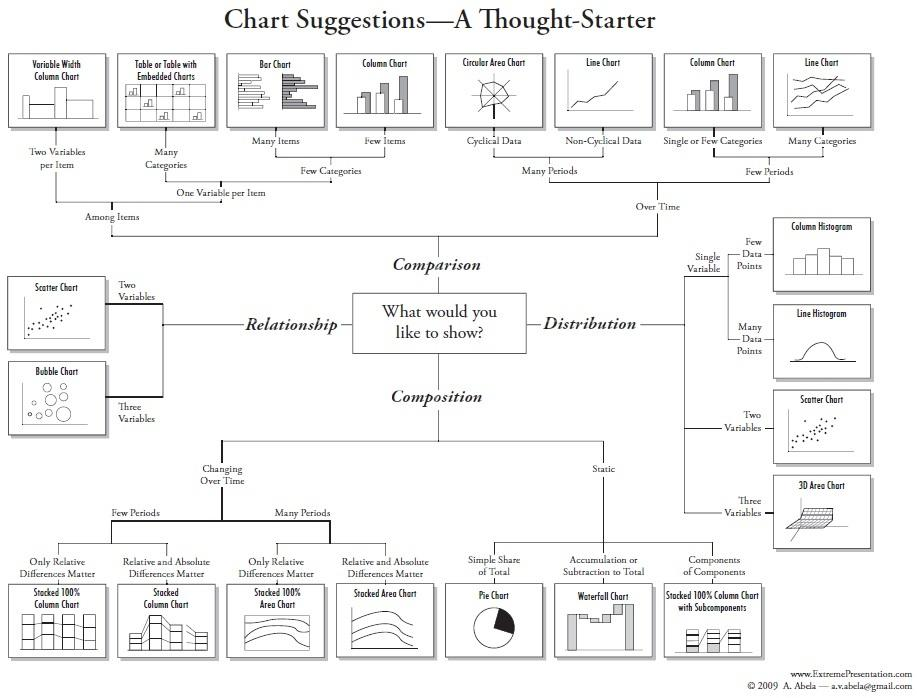
\includegraphics[width=\textwidth]{images/which-chart-when.jpeg}
\caption{Visualisation}
\end{figure}

\URL{https://github.com/d3/d3/wiki/Gallery}

\section{Software Projects}\label{software-projects}

\textbf{Contents}

Please read the information in the overview page at

\begin{itemize}
\tightlist
\item
  \url{http://bdaafall2016.readthedocs.io/en/latest/overview.html\#software-project}
\end{itemize}

After doing so please return to this page. Identify a project suitable
for this class, propose it and work on it.

There are several categories of software projects, which are detailed in
lower sections:

\begin{enumerate}
\tightlist
\item
  Deployment
\item
  Analytics
\end{enumerate}

You may propose a project in one of these categories, if you are doing a
software projects.

These are non-trivial project and involve substantial work. Many
students vastly underestimate the difficulty and the amount of time
required. This is the reason why the project assignment is early on in
the semester so you have ample time to propose and work on it. If you
start the project 2 weeks before December (Note the early due data) We
assume you may not finish.

\subsection{Common Requirements}\label{common-requirements}

All software projects must:

\begin{enumerate}
\item
  Be submitted via gitlab (a repository will be created for you)
\item
  Be reproducibly deployed

  Assume you are given a username and a set of IP addresses. From this
  starting point, you should be able to deploy everything in a single
  command line invocation.

  Do not assume that the username or IP address will be the ones you use
  during development and testing.
\item
  Provide a report in the \texttt{docs/report} directory

  LaTeX or Word may be used. Include the original sources as well as a
  PDF called \texttt{report.pdf} (See overview-software-project for
  additional details on the report format. You will be using 2 column
  ACM format we have used before.)
\item
  Provide a properly formatted \texttt{README.rst} or \texttt{README.md}
  in the root directory

  The README should have the following sections:

  \begin{itemize}
  \tightlist
  \item
    Authors: list the authors
  \item
    Project Type: one of ``Deployment'', ``Analytics''
  \item
    Problem: describe the task and/or problem
  \item
    Requirements: describe your assumptions and requirements for
    deployment/running. This should include any software requirements
    with a link to their webpage. Also indicate which versions you have
    developed/tested with.
  \item
    Running: describe the steps needed to deploy and run
  \item
    Acknowledgements: provide proper attribution to any websites, or
    code you may have used or adapted
  \end{itemize}

  \begin{description}
  \item[in the past we got projects that had 10 pages]
  installation instructions. Certainly that is not good and you will get
  point deductions. The installation should be possible in a couple of
  lines. A nice example is the installation of the development software
  in the ubuntu vm. Naturally you can use other technologies, other than
  ansible. Shell scrips, makefiles, python scripts are all acceptable.
  \end{description}
\item
  A \texttt{LICENSE} file (this should be the \texttt{LICENSE} for
  Apache License Version 2.0)
\item
  All figures should include labels with the following format:
  \texttt{label\ (units)}.

  For example:

  \begin{itemize}
  \tightlist
  \item
    \texttt{distance\ (meters)}
  \item
    \texttt{volume\ (liters)}
  \item
    \texttt{cost\ (USD)}
  \end{itemize}
\item
  All figures should have a caption describing what the measurement is,
  and a summary of the conclusions drawn.

  For example:

  \begin{quote}
  This shows how A changes with regards to B, indicating that under
  conditions X, Y, Z, Alpha is 42 times better than otherwise.
  \end{quote}
\end{enumerate}

\subsection{Deployment Projects}\label{deployment-projects}

Deployment projects focuses on automated software deployments on
multiple nodes using automation tools such as Ansible, Chef, Puppet,
Salt, or Juju. You are also allowed to use shell scripts, pdsh, vagrant,
or fabric. For example, you could work on deploying Hadoop to a cluster
of several machines. Use of Ansible is recommended and supported. Other
tools such as Chef, Puppet, etc, will not be supported.

Note that it is not sufficient to merely deploy the software on the
cluster. You must also demonstrate the use of the cluster by running
some program on it and show the utilization of your entire cluster. You
should also benchmark the deployment and running of your demonstration
on several sizes of a cluster (eg 1, 3, 6, 10 nodes) (Note that these
numbers are for example only).

We expect to see figures showing times for each (deployment, running)
pair on for each cluster size, with error bars. This means that you need
to run each benchmark multiple times (at least three times) in order to
get the error bars. You should also demonstrate cluster utilization for
each cluster size.

The program used for demonstration can be simple and straightforward.
This is not the focus of this type of project.

\subsection{IaaS}\label{iaas}

It is allowable to use

\begin{itemize}
\tightlist
\item
  virtualbox
\item
  chameleon cloud
\item
  futuresystems
\item
  AWS (your own cost)
\item
  Azure (your own cost)
\end{itemize}

for your projects. Note that on powerful desktop machines even
virtualbox can run multiple vms. Use of docker is allowed, but you must
make sure to use docker properly. In the past we had students that used
docker but did not use it in the way it was designed for. Use of docker
swarm is allowed.

\subsubsection{Requirements}\label{requirements}

Deployment projects must include a repeatable deployment framework that
uses cmd5 and ansible. When using ansible it should be called from a
custoom cmd5 program.

\subsubsection{Example projects}\label{example-projects}

See also
\url{https://docs.google.com/document/d/1KylDsRBmVbCZSqGpRbzYwdzUGKFi92bkATwU03of5gw}

\begin{itemize}
\tightlist
\item
  deploy Apache Spark on top of Hadoop
\item
  deploy Apache Pig on top of Hadoop
\item
  deploy Apache Storm
\item
  deploy Apache Flink
\item
  deploy a Tensorflow cluster
\item
  deploy a PostgreSQL cluster
\item
  deploy a MongoDB cluster
\item
  deploy a CouchDB cluster
\item
  deploy a Memcached cluster
\item
  deploy a MySQL cluster
\item
  deploy a Redis cluster
\item
  deploy a Mesos cluster
\item
  deploy a Hadoop cluster
\item
  deploy a docker swarm cluster
\item
  deploy NIST Fingerprint Matching
\item
  deploy NIST Human Detection and Face Detection
\item
  deploy NIST Live Twitter Analysis
\item
  deploy NIST Big Data Analytics for Healthcare Data and Health
  Informatics
\item
  deploy NIST Data Warehousing and Data mining
\end{itemize}

Deployment projects must have EASY installation setup just as we
demonstrated in the ubuntu image.

A command to manage the deployment must be written using python docopts
that than starts your deployment and allows management of it. You can
than from within this command call whatever other framework you use to
manage it. The docopts manual page should be designed first and
discussed in the team for completeness.

Using argparse and other python commandline interface environments is
not allowed.

Deployment project will not only deply the farmewor, but either provide
a sophisticated benchmark while doing a simple analysis using the
deployed software.

\subsection{Analytics Projects}\label{analytics-projects}

Analytics projects focus on data exploration. For this type of projects,
you should focus on analysis of a dataset (see datasets for starting
points). The key here is to take a dataset and extract some meaningful
information from in using tools such as \texttt{scikit-learn},
\texttt{mllib}, or others. You should be able to provide graphs,
descriptions for your graphs, and argue for conclusions drawn from your
analysis.

Your deployment should handle the process of downloading and installing
the required datasets and pushing the analysis code to the remote node.
You should provide instructions on how to run and interpret your
analysis code in your README.

\subsubsection{Requirements}\label{requirements-1}

An analytocs project may focus on a sophisticated and academically
correct usage of an analytics of data. It must be significant and not
just a simple replication of what others have done before.

\subsubsection{Example projects}\label{example-projects-1}

\begin{itemize}
\tightlist
\item
  analysis of US Census data
\item
  analysis of Uber ride sharing GPS data
\item
  analysis of Health Care data
\item
  analysis of images for Human Face detection
\item
  analysis of streaming Twitter data
\item
  analysis of airline prices, flights, etc
\item
  analysis of network graphs (social networks, disease networks, protein
  networks, etc)
\item
  analysis of music files for recommender engines
\item
  analysis of NIST Fingerprint Matching
\item
  analysis of NIST Human Detection and Face Detection
\item
  analysis of NIST Live Twitter Analysis
\item
  analysis of NIST Big Data Analytics for Healthcare Data and Health
  Informatics
\item
  analysis of NIST Data Warehousing and Data mining
\item
  author disambiguity problem in academic papers
\item
  application of a k-means algorithm
\item
  application of a MDS
\end{itemize}

\subsection{Project Idea: World wide road
kill}\label{project-idea-world-wide-road-kill}

This project can also be executed as bonus project to gather information
about the feasability of existing databases.

It would be important to identify also how to potentially merge these
databases into a single world map and derive statistics from them. This
project can be done on your local machines. Not more than 6 people can
work on this.

Identify someone that has experience with android and/or iphone
programming Design an application that preferably works on iphone and
android that allows a user while driving to

\begin{itemize}
\tightlist
\item
  call a number to report roadkill via voice and submitting the gps
  coordinates
\item
  have a button on the phone that allows the gps coordinates to be
  collected and allow upload either live, or when the user presses
  another butten.
\item
  have provisions in the application that allow you to augment the data
\item
  have an html page that displays the data
\item
  test it out within users of this class (remember we have world wide
  audience)
\end{itemize}

Make sure the app is ready early so others can test and use it and you
can collect data.

Before starting the project identify if such an application already
exists.

If more than 6 people sign up we may build a second group doing
something similar, maybe potholes ..

Gregor would like to get this project or at least the database search
query staffed.

\subsection{Project Idea: Author disambiguty
problem}\label{project-idea-author-disambiguty-problem}

Given millions of publications how do we identify if an author of paper
a with the name Will Smith is the sam as the author of paper 2 with the
name Will Smith, or William Smith, or W. Smith. AUthor databases are
either provided in bibtex format, or a database that can not be shared
outside of this class. YOu may have to add additional information from
IEEE explorer, rsearch gate, ISI, or other online databases.

Identify further issues and discuss solutions to them. Example, an
author name changes, the author changes the institution.

Do a comprehensive literature review

Some ideas:

\begin{itemize}
\tightlist
\item
  Develop a graph view application in JS that showcases dependencies
  between coauthors, institutions
\item
  Derive probabilities for the publications written by an auther given
  they are the same
\item
  Utilize dependency graphs as given by online databases
\item
  Utilize the and or topic/abstarct/full text to identify similarity
\item
  Utilize keywords in the title
\item
  Utilize refernces of the paper
\item
  Prepare some vizualization of your result
\item
  Prepare som interactive vizualization
\end{itemize}

A possible good start is a previous project published at

\begin{itemize}
\tightlist
\item
  \url{https://github.com/scienceimpact/bibliometric}
\end{itemize}

There are also some screenshots available:

\begin{itemize}
\tightlist
\item
  \url{https://github.com/scienceimpact/bibliometric/blob/master/Project\%20Screenshots/Relationship_Authors_Publications.PNG}
\item
  \url{https://github.com/scienceimpact/bibliometric/blob/master/Project\%20Screenshots/Relationship_Authors_Publications2_Clusters.PNG}
\end{itemize}


\end{comment}

%\part{Linux}
%

\chapter{Linux}
\label{C:linux}

\FILENAME

\section{History}

LINUX is a reimplementation by the community of UNIX which was
developed in 1969 by Ken Thompson and Dennis Ritchie of Bell
Laboratories and rewritten in C. An important part of UNIX is what is
called the {\em kernel} which allows the software to talk to
the hardware and utilize it. 

In 1991 Linus Trovalds started developing a Linux Kernel that was
initially targeted for PC's. THis made it possible to run it on
Laptops and was later on further developed by making it a full
Operating system replacement for UNIX. 

\section{Shell}

One of the most important features for us will be to access the
computer with the help of a {\em shell}. THe shell is typically run in
what is called a terminal and allows interaction to the computer with
commandline programs. 

There are many good tutorials out there that explain why one needs a
linux shell and not just a GUI. Randomly we picked the first one that
came up with a google query (This is not an endorsement for the material
we point to, but could be a worth while read for someone that has no
experience in Shell programming:

\URL{http://linuxcommand.org/lc3_learning_the_shell.php}

Certainly you are welcome to use other resources that may suite you
best. We will however summarize in table form a number of useful
commands that you may als find even as a RefCard.

\URL{http://www.cheat-sheets.org/\#Linux}

We provide in Table \ref{T:shell-commands} a number of useful commands
that you want to explore. For more information simply type man and the
name of the command.


\begin{center}
\begin{longtable}{|p{4cm}|p{8cm}|}
\caption{Common commands}\label{T:shell-commands}\\

\hline
\multicolumn{1}{|p{4cm}|}{\textbf{Example}} & \multicolumn{1}{p{8cm}|}{\textbf{Description}} \\ 
\hline 
\endfirsthead

\multicolumn{2}{p{12cm}}%
{{\bfseries \tablename\ \thetable{} -- continued from previous page}} \\
\hline 
\hline \multicolumn{1}{|p{4cm}|}{\textbf{Example}} & \multicolumn{1}{p{8cm}|}{\textbf{Description}} \\ 
\hline 
\endhead

\hline 
\multicolumn{2}{|r|}{{Continued on next page}} \\
\hline
\endfoot

%\hline 
\hline
\endlastfoot

  \multicolumn{2}{|l|}{\cellcolor{blue!15} Help Commands}\\
  \hline
  man \emph{command} & manual page for the \emph{command} \\
  apropos {\em text} & list all commands that have text in it\\
  & \\

  \hline
  \multicolumn{2}{|l|}{\cellcolor{blue!15} File Commands}\\
  \hline
  ls & Directory listing\\
  ls -lisa & list details \\
  tree & list the directories in graphical form \\
  cd \emph{dirname} & Change directory to \emph{dirname} \\
  mkdir \emph{dirname} & create the directory \\
  pwd & print working directory \\
  rm \emph{file} & remove the file \\
  cp \emph{a} \emph{b} & copy file \emph{a} to \emph{b} \\
  mv \emph{a} \emph{b} & move/rename file \emph{a} to \emph{b}\\
  cat \emph{a} & print content of file\emph{a}\\
  cat - n &  (assignment) \\
  less \emph{a} & print paged content of file \emph{a}\\
  head -5 \emph{a} & Display first 5 lines of file \emph{a}\\
  tail -5 \emph{a} & Display last 5 lines of file \emph{a}\\
  du -hs . & show in human readable form the space used by the current
             directory\\
  wc {\em filename} &  counts the word in a file \\
  sort {\em filename} &  sorts the file \\
  tar -xvf {\em dir} &  tars up a compressed version of the directory \\
  rsync &  (assignment) \\
  gzip &  (assignment) \\
  bzip2 &  (assignment) \\
  & \\
  
  %\hline
  %\multicolumn{2}{|l|}{\cellcolor{blue!15} Search Commands}\\
  %\hline
  chmod go-rwx {\em file} & changes the permission of the file \\
  chown {\em username} {\em file} & changes the ownership of the file \\
  chgrp {\em group} {\em file} & changes the group of a file\\
  & \\

  \hline
  \multicolumn{2}{|l|}{\cellcolor{blue!15} Search Commands}\\
  \hline
  fgrep ``text'' filename &  searches the text in the given file \\
  grep -R ``xyz'' . & recursively searches for xyz in all files \\
  find . -name ``*.py'' &  find all files with .py at the end \\
  & \\

  %\hline
  %\multicolumn{2}{|l|}{\cellcolor{blue!15} Process Commands}\\
  %\hline
  ps & list the running processes \\
  kill -9 1234 & kill the process with the id 1234 \\
  at &  (assignment) \\
  cron &  (assignment) \\
  crontab &  (assignment) \\
  & \\

  \hline
  \multicolumn{2}{|l|}{\cellcolor{blue!15} Device Commands}\\
  \hline
  mount /dev/cdrom /mnt/cdrom & mount a filesystem from a cd rom to /mnt/cdrom\\
  & \\

  \hline
  \multicolumn{2}{|l|}{\cellcolor{blue!15} System Commands}\\
  \hline
  users &  (assignment) \\
  who &  (assignment) \\
  whoami &  (assignment) \\
  dmesg &  (assignment) \\
  last &  (assignment) \\
  free -tm &  (assignment) \\
  uname &  (assignment) \\
  date &  prints the current date and time \\
  time {\em &  (assignment) \\
  shutdown -h ``shut down'' & (assignment) \\
  & \\

  \hline
  \multicolumn{2}{|l|}{\cellcolor{blue!15} Networking Commands}\\
  \hline
  ping &  (assignment) \\
  netstat &  (assignment) \\
  hostname &  (assignment) \\
  traceroute &  (assignment) \\
  ifconfig &  (assignment) \\
  & \\

  \hline
  \multicolumn{2}{|l|}{\cellcolor{blue!15} Internet Commands}\\
  \hline
  host &  (assignment) \\
  whois &  (assignment) \\
  dig &  (assignment) \\
  wget &  (assignment) \\
  curl &  (assignment) \\
  & \\

  \hline
  \multicolumn{2}{|l|}{\cellcolor{blue!15} Remote Access Commands}\\
  \hline
  ssh &  (assignment) \\
  scp &  (assignment) \\
  sftp &  (assignment) \\
  & \\


\end{longtable}
\end{center}

\section{Multi-command execution}

One of the important features is that one can execute multiple
commands in the shell.

To execute command 2 once command 1 has finished use

\begin{verbatim}
command1; command2
\end{verbatim}

To execute command 2 as soon as command 1 forwards output to stdout use

\begin{verbatim}
command1; command2
\end{verbatim}

To execute command 1 in the background use

\begin{verbatim}
command1 &
\end{verbatim}



\section{Keyboard Shortcuts}\label{keyboard-shortcuts}

These shortcuts will come in handy. Note that many overlap with emacs
short cuts.

\begin{tabular}{ll}
Keys     & Description  \\
\hline
Up Arrow & Show the previous command\\
Ctrl + z & Stops the current command  \\
         & Resume with fg in the foreground \\
         & Resume with bg in the background \\
Ctrl + c & Halts the current command\\
Ctrl + l & Clear the screen\\
Ctrl + a & Return to the start of the line\\
Ctrl + e & Go to the end of the line\\
Ctrl + k & Cut everything after the cursor to a special clipboard\\
Ctrl + y & Paste from the special clipboard \\
Ctrl + d & Log out of current session, similar to exit \\
\end{tabular}

\section{.bashrc and .bash\_profile}\label{bashrc-and-.bash_profile}

Usage of a particular command and all the attributes associated with it,
use `man' command. Avoid using \verb|rm -r| command to delete files
recursively. A good way to avoid accidental deletion is to include the
following in your \verb|.bash_profile| file:

\begin{verbatim}
alias e=open_emacs
alias rm='rm -i'
alias mv='mv -i' 
alias h='history'
\end{verbatim}

More Information

\url{https://cloudmesh.github.io/classes/lesson/linux/refcards.html}

\section{Exercise}

\begin{description}
\item[Linux.1:]
Familiarize yourself with the commands
\item[Linux.2:]
Find more commands that you find useful and add them to this page.
\item[Linux.3:]
Use the sort command to sort all lines of a file while removing
duplicates.
\item[Linux.4:] In Table \ref{T:shell-commands} you will find a number
  of commands with (assignment). Develop descriptions that you will
  contribute and add to the manual with a pull request. Work in a team
  so that only one pull request is issued. Do not only provide the
  description, but also a real example as showcased within the table.
\item[Linux.4:] Should there be other commands listed in the table. If
  so which? Create a pull request for them. 
\end{description}


%%----------------------------------------------------------------------------------------
%	PART
%----------------------------------------------------------------------------------------

\part{Documenting Scientific Research}



%----------------------------------------------------------------------------------------
%	CHAPTER 1
%----------------------------------------------------------------------------------------

\chapterimage{writing.png} % Chapter heading image

\chapter{Documenting Scientific Research}
\label{c:doc}

\FILENAME

\FILENAME

\section{Plagiarism}\label{S:plagiarism}

We start with the review of a most important topic.

\subsection{Plagiarism Definition}

In academic life it is important to understand and avoid plagiarism.
The dictionary defines plagiarism as follows \url{dictionary.com}:

% \textipa{['pl\=aj@""riz@m]}

\begin{description}
\item[pla·gia·rism] ``the practice of taking someone else's work or ideas and passing them
off as one's own.''
\end{description}



\subsection{Plagiarism Policies}
Organizations and universities will have policies in place do address
plagiarism. An example is provided for Indiana University
\cite{www-iu-plagiarism}. We quote:

\begin{quotation}
``Honesty requires that any ideas or materials taken from
another source for either written or oral use must be fully
acknowledged. Offering the work of someone else as one’s own is
plagiarism. The language or ideas thus taken from another may range
from isolated formulas, sentences, or paragraphs to entire articles
copied from books, periodicals, speeches, or the writings of other
students. The offering of materials assembled or collected by others
in the form of projects or collections without acknowledgment also is
considered plagiarism. Any student who fails to give credit for ideas
or materials taken from another source is guilty of plagiarism. 

(Faculty Council, May 2, 1961; University Faculty Council, March 11,
1975; Board of Trustees, July 11, 1975)''
\end{quotation}

Faculty members at Universitys are also bound by policies that mandate
reporting. At Indiana University the following policy applies (for a
complete policy see the Web page):

\begin{quotation}
``Should
the faculty member detect signs of plagiarism or cheating, it is his
or her most serious obligation to investigate these thoroughly, to
take appropriate action with respect to the grades of students, and
\textit{in any event} to report the matter to the Dean for Student Services [or
equivalent administrator]. The necessity to report every case of
cheating, whether or not further action is desirable, arises
particularly because of the possibility that this is not the student’s
first offense, or that other offenses may follow it. Equity also
demands that a uniform reporting practice be enforced; otherwise, some
students will be penalized while others guilty of the same actions
will go free.

(Faculty Council, May 2, 1961)''
\end{quotation}

Naturally if a student has any questions about understanding
plagiarism the University can provide assistance. If a student is in
doubt and asks for help this is not considered at that time
plagiarism. 

As you can see from the previous policies, the faculty do not have any
choice but reporting real cases of plagiarism to the university
administration.  Thus you must not hold them personally responsible as
this is part of the tasks they are required to do if they like it or
not. Instead, it is {\bf the responsibility of the authors of the
  document} to assure no plagiarism occurs. If you are a student of a
class that writes a paper or project report this naturally also all
applies to you. In addition, if you work in a team you need to assure
the entire team addresses plagiarism appropriately.

In practice this means that the teachers of a course expect yo know
plagiarism and you need to be informed about it. This is typically
done in other courses. However, as it is often overlooked by the
student we are pointing it out here so we can make sure you contribute
to courses that require you to write papers and reports. This also
means you can not claim you did not know what plagiarism is. You are
required to know what it is, know how to detect it and know how to
avoid it. The resources provided next will give you the necessary
tools and background.

\subsection{Plagiarism Resources}

The \href{http://education.indiana.edu/}{School of Education at Indiana
University} has a significant set of resources to get educated about
plagiarism. These resources are intended to ``preparing educators,
advancing knowledge, and improving education'' \cite{}
\url{https://www.indiana.edu/~istd/patterns.html}

The content here is copied from the Web Page

  \URL{https://www.indiana.edu/~istd/patterns.html}

As such we have not included quotes but refer to their Web page for the
original source which may also include updates. Naturally we do not want
to be accused of plagiarize in a chapter about plagiarism.  Thus assume
the content for the rest ov this chapter are copied from that Web page.

\subsection{Pattern}\label{pattern}

\begin{itemize}
\item
  \href{https://www.indiana.edu/~istd/definition.html}{IU Definition} of
  Plagiarism from Student Code of Conduct
\item
  \href{https://www.indiana.edu/~istd/overview.html}{Overview} How to
  give proper credit, steps.
\item
  \href{https://www.indiana.edu/~istd/cases.html}{Cases} of Plagiarism
  in the US, in the news, and elsewhere
\item
  \href{https://www.indiana.edu/~istd/examples.html}{Examples} Word for
  word, paraphrasing
\item
  \href{https://www.indiana.edu/~istd/practice.html}{Practice} with
  feedback on word-for-word and paraphrasing plagiarism
\item
  \href{https://www.indiana.edu/~istd/test.html}{Test} 10 questions on
  recognizing plagiarism
\item
  \href{https://www.indiana.edu/~istd/sitemap.html}{Tutorial Site Map}
  Expanded table of contents
\item
  \href{https://www.indiana.edu/~istd/resources.html}{Resources}
  Websites, books, dictionary links, references for learning more about
  plagiarism
\end{itemize}

\subsection{Tutorials}\label{S:ptutorial}

A number of tutorials are offerd by Indiana University \href{http://education.indiana.edu/graduate/programs/instructional-systems/index.html}{Instructional
  Systems Technology Department}
 Web pages ealing with plagiarism. Thes include:

\begin{itemize}
\item
  \href{https://www.indiana.edu/~academy/firstPrinciples/choice.html}{Plagiarsim
    Tutorial}
\item
  \href{https://www.indiana.edu/~tedfrick/plagiarism/}{Understanding
  Plagiarism}
\end{itemize}

\subsection{How to Recognize Plagiarism}

We are listing fifteen patterns of plagiarism that are defined on the Web
pages itedntified in Section~\ref{S:ptutorial}:

\begin{tabular}{p{4cm}p{3cm}p{8cm}}
Name & Plagiarism Type & Reason \\
\hline
  \href{patternCluelessQuote.html}{Clueless Quote} &  word-for-word & no
  quotes, no citation, no reference 
\\
  \href{patternCraftyCoverUp.html}{Crafty Cover-up} &  proper paraphrase
  but word-for-word  &  also present
\\
  \href{patternCunningCoverUp.html}{Cunning Cover-up} &  paraphrasing & no
  citation, no reference
\\
  \href{patternDeceptiveDupe.html}{Deceptive Dupe} &  word-for-word  &  no
  quotes, no citation, but has reference
\\
  \href{patternDisconnectedDupe.html}{Delinked Dupe} &  word-for-word  &  no
  reference, even though quotes and citation
\\
  \href{patternDeviousDupe.html}{Devious Dupe} &  correct quote but word-for-word  & 
  also present
\\
  \href{patternDippyDupe.html}{Dippy Dupe} &  word-for-word  &  quotes
  missing, even though full citation and reference
\\
  \href{patternDisguisedDupe.html}{Disguised Dupe} &  looks like proper
  para, but actually word-for-word  &  no quotes, no locator
\\
  \href{patternDoubleTrouble.html}{Double Trouble} & word-for-word  and
  paraphrasing  & although has reference
\\
  \href{patternLostLoser.html}{Linkless Loser} &  word-for-word  &  citation
  and reference lacking, although has quotes and locator
\\
  \href{patternLostLocator.html}{Lost Locator} &  word-for-word  &  missing
  locator, although has quotes, citation, and reference
\\
  \href{patternPointlessParaphrase.html}{Placeless Paraphrase} &  paraphrasing  & 
  no reference, although citation present
\\
  \href{patternSeveredCite.html}{Severed Cite} &  paraphrasing  &  reference
  but no citation
\\
  \href{patternShirkingCite.html}{Shirking Cite} &  word-for-word  &  lacks
  locator and reference, although quotes and citation present
\\
  \href{patternTripleD.html}{Triple D--Disguised Disconnected Dupe} & 
  word-for-word  & looks like proper para, but no quotes, no reference, no locator
\end{tabular}

In addition they do specify  three patterns of
non-plagiarism:

\begin{tabular}{p{2cm}p{4cm}p{8cm}}
Name & Type & Description \\
\hline
\\
  \href{patternCorrectQuote.html}{Correct Quote} &  non-plagiarizm & takes another's words
  verbatim and acknowledges with quotation marks, full in-text citation
  with locator, and reference
\\
  \href{patternProperParaphrase.html}{Proper Paraphrase} &  non-plagiarizm & summarizes
  another's words and acknowledges with in-text citation and reference
\\
  \href{patternMindlessParaphrase.html}{Parroted Paraphrase} &  non-plagiarizm & appears to
  be paraphrasing, and technically may not be plagiarism, but \ldots{}
  ???
\end{tabular}


\FILENAME

\section{Acknowledgements}
\label{S:acknowledgements}

In many cases you want to include an acknowledgement section. In some cases you may be tempted to eliminate this section as you think you are out of space and the acknowledgement section may give you some additional space. This however is the wrong strategy and you should not do this. Instead you should shorten your paper elsewhere and leave enough space for acknowledgements.

In some cases where you get financial support from a university for a project such as from NIH or NSF specific information {\bf must} be included. The best way is to verify with your coauthors. Additional acknowledgements may have to be added and you need te evaluate if for example significant help on the paper warrants co-authorship.

An issue that we have seen often is for example when a professor has helped significantly on the paper but is not properly acknowledged. This can even lead to the professor asking you to remove him from the acknowledgement. A bad acknowledh]gement example is the following:

\begin{quote}
We like to thank Professor Zweistein for his help in compiling  the \LaTeX paper.
\end{quote}

We do not think that the professor will be happy with this acknowledgement as it sounds like the only thing that was provided was the help on LaTeX that you should have done anyways without the help of the professor. Ask yourself, if he introduced you to the field, has helped you with preparing the text, has given you insights, has corrected things in your paper, made suggestions. So instead of the above maybe a more general term such as {\em helped with the paper} would be more appropriate. If not leaving it off is more appropriate. In some cases you may wan to invite your professor to become a co-author. 

\FILENAME

\section{Writing a Scientific Article or Conference Paper}
\index{Writing}

An important part of any scientific research is to document it. This is
often done through scientific conferences or journal articles. Hence it
is important to learn how to prepare and submit such papers. Most
conferences accept typically the papers in PDF format but require the
papers to be prepared on MSWord or in LaTeX. While working with many
students in the past we noticed however that those students using Word
often spend unnecessarily countless hours on trying to make there papers
beautiful while actually violating the template provided by the
conference. Furthermore, we noticed that the same students had issues
with bibliography management. Instead of Word helping the student it
provided the illusion to be easier than LaTeX but when adding up the
time spend on the paper we found that LaTeX actually saved time. This
has been especially true with the advent of collaborative editing
services such as sharelatex \cite{www-sharelatex} and overleaf
\cite{www-overleaf}. 

In this section we provide you with a professional template that is used
for either system based on the ACM standard that you can use to write
papers. Naturally this will be extremely useful if the quality of your
research is strong enough to be submitted to a conference. We structure
this section as follows. Although we do not recommend that you use
MSWord for your editing of a scientific paper, we have included a short
section about it and outline some of its pitfalls that initially you may
not think is problematic, but has proven to be an issue with students.
Next we will focus on introducing you to LaTeX and showcasing you the
advantages and disadvantages. We will dedicate an entire section on
bibliography management and teach you jhow to use jabref which clearly
has advantages for us.

Having a uniform report format not only helps the students but allow
allows the comparison of paper length and effort as part of teaching a
course. We have added an entire section to this chapter that discusses
how we can manage a \emph{Class Proceedings} form papers that are
contributed by teams in the class.

\subsection{Professional Paper Format}\label{professional-paper-format}

The report format we suggest here is based on the standard ACM
proccedings format. It is of very high quality and can be adapted for
your own activities. Moreover, it is possible to use most of teh text to
adapt to other formats in case the conference you intend to submit your
paper to has a different format. The ACM format is always a good start.

Important is that you do not need to change the template but you can
change some parameters in case you are not submitting the paper to a
conference but use it for class papers. Certainly you should not change
the spacing or the layout and instead focus on writing content. As for
bibliography management we recommend you use jabref which we will
introduce in Section \ref{??}.

We recommend that you carefully study the requirements for the report
format. We would nat want that your paper gets rejected by a journal,
conference or the class just because you try to modify the format or do
not follow the established publication guidlines.

The template we are providing is available from:

\URL{https://github.com/cloudmesh/classes/tree/master/docs/source/format/report}

Convenient compressed files are available at

\URL{https://github.com/cloudmesh/classes/tree/master/docs/source/format/report.tar.gz}
\URL{https://github.com/cloudmesh/classes/tree/master/docs/source/format/report.zip}

You will find in it a modified ACM proceedings templates for Word and
for LaTeX that has an identification box removed on the lower left hand
side of the first page. This is done for classes so that you have more
space to write. In case you must submit to a conference you can use the
original ACM template. This template can be found at

\subsection{Submission Requirements}\label{submission-requirements}

Although the initial requirement for some conferences or journals is the
document PDF, in many cases you must be prepared to provide the source
when submitting to the conference. This includes the submission of the
original images in an images foder. You may ba asked to package the
document into a folder with all of its sources and submit to the
conference for professional publication.

\subsection{Microsoft Word vs. \LaTeX}\label{microsoft-word}

Microsoft word will provide you with the initial impression that you
will safe lots of time writing in it while you see the layout of the
document. This will be initially true, but once you progress to the
more challenging parts and later pages such as image menagement and
bibliography management you will see some issues. Thes include that
figure placement in Word need sto be done just right in order for images
to be where they need. We have seen students spending hours with the
placement of figures in a paper but when they did additional changes the
images jumped around and were not at the place where teh students
expected them to be. So if you work with images, make sure you
understand how to place them. Also always use relative caption counters
so that if an image gets placed elsewhere the counter stays consistent.
So nefer use just the number, but a reference to the figure when referring
to it. Recently a new bibliography management system was added to Word.
However, however it is not well documented and the references are placed
in the system bibliography rather than a local managed bibliography.
This mah have severe consequences when working with many authors on a
paper. The same is true when using Endnote. We have heard in many
occasions that the combination of endnote and Word destroyed documents.
You certainly do not want that to happen the day before your deadline.
Also in classes we observed that those using LaTeX deliver better
structured and written papers as the focus is on text and not beautiful
layout.

For all these reasons we do not recommend that you use Word.

In LaTeX where we have an easier time with this as we can just ignore
all of these issues due to relative good image placement and excellent
support for academic reference management. Hence, it is in your best
interest to use LaTeX. The information we provide here will make it easy
for you to get started and write a paper in no time as it is just like
filling out a form.

\subsection{Working in a Team}\label{working-in-a-team}

Today research is done in potentially large research teams. This also
include the writing of a document. There are multiple ways this is done
these days and depends on the system you chose.

In MSWord you can use skydrive, while for LaTeX you can use sharelatex
and overleaf. However, in many cases the use of github is possible as
the same groups that develop the code are also familiar with github.
Thus we provide you here also with the introduction on how to write a
document in github while group members can contribute.

Here are the options:

\begin{description}

\item [LaTeX and git:] This option will likely safe you time as you can use
  jabref also for managing collaborative bibliographies and
\item [sharelatex:] an online tool to write latex documents
\item [overleaf:] an online tool to write latex documents
\item [MS onedrive:] It allows you to edit a word document in collaboration.
  We recommend that you use a local installed version of Word and do the
  editing with that, rather than using the online version. The online
  editor has some bugs. See also (untested):
  \url{http://www.paulkiddie.com/2009/07/jabref-exports-to-word-2007-xml/},
  \url{http://usefulcodes.blogspot.com/2015/01/using-jabref-to-import-bib-to-microsoft.html}
\item [Google Drive:] google drive could be used to collaborate on text that
  is than pasted into document. However it is just a starting point as
  it does not support typically the format required by the publisher.
  Hence at one point you need to swithc to one of the other systems.
\end{description}

\subsection{Timemanagement}\label{timemanagement}

Obviously writing a paper takes time and you need to car-fully make sure
you devote enough time to it. The important part is that the paper
should not be an after thought but should be the initial activity to
conduct and execute your research. Remember that

\begin{enumerate}

\item  It takes time to read the information
\item  It takes time understand the information
\item  It takes time to do the research

\end{enumerate}

For deadlines the following will get you in trouble:

\begin{enumerate}

\item
  \emph{There are still 10 weeks left till the deadline, so let me start
  in 4 week \ldots{}}. Procrastination is your worst enemy.
\item
  If you work in a team that has time management issues address them
  immediately
\item
  Do not underestimate the time it takes to prepare the final submission
  into the submission system. Prepare automated scripts that can deliver
  the package for submission in minutes rather than hours by hand.
\end{enumerate}

\subsection{Paper and Report Checklist}\label{paper-checklist}
\index{Writing!Checklist}

In this section we summarize a number of checks that you may perform to
make sure your paper is properly formatted and in excellent shape.
Naturally this list is just a partial list and if you find things we
should add here, let us know.

\begin{itemize}[label=$\Box$]

\item Have you written the report in the specified format?

\item Have you included an acknowledgement section?

\item Have you included the paper in the submission system (In our
  case git). This includes all images, bibliography files and other
  material that is needed to build the paper from scratch?

\item Have you added the bibliography file that you managed (In our
  case jabref to make it simple for you)?

\item Have you specified proper identification in the submission
  system for your submission.  This is typically a form or ASCII text
  that needs to be filled out and follows a very particular format.
  In our case it is a README.md file that ncludes a homework ID, names
  of the authors, and e-mails)?

\item In case you used word have you also provided the jabref?

\item In case of a class and if you do a multi-author paper, have you
  added a work-breakdown section in the appendix describing who did
  what in the paper?

\item IN case you have an appenix it is included fater the bibliography

\item Have you spellchecked the paper?

\item Have you grammar chacked the paper?

\item Are you using \textbf{a} and \textbf{the} properly?

\item Have you made sure you do not plagiarize?

\item Is the title properly capitalized?

\item Have you not used phrases such as shown in the Figure below, but
  instead used as shown in Figure 3 when referring to the 3rd figure?
  Numbers in LaTeX are done with \verb|\label{}| after captions and
  \verb|\ref{}| in the text (See examples in the LaTeX section). In
  word you must use relative numbering.

\item Have you capitalized ``Figure 3'', ``Table 1''?

\item Have you removed any figure that is not referred explicitly in
  the text. E. ech figure needs a text such as  {\em As shown in
    Figure ..} or similar.

\item Are the figure captions bellow the figures and not on top. (Do
  not include the titles of the figures in the figure itself but
  instead use the caption or that information?

\item When using tables have you put the table caption above the table?

\item When using image have you put the table caption bellow the image?

\item Make the figures large enough so we can read the details. If
  needed make the figure over two columns? 

\item Do not worry about the figure placement if they are at a
  different location than you think. Figures are allowed to float. In
  many submissions you may have to place all figures at the end of the
  paper so you can focus on content rather than placing figures. In
  addition it will help you to refer to the figures by index.

\item Are all figures and tables at the end?

\item In case you copied a figure from another paper you need to ask
  for copyright permission. In case of a class paper you \textbf{must}
  include a reference to the original at the end of the figure caption.

\item Do not use the word ``I'' instead use ``we'' even if you are the
  sole author.

\item Do not use the phrase ``In this paper/report we show'' instead
  use ``We show''. It is not important if this is a paper or a report
  and does not need to be mentioned.

\item Do not artificially inflate your paper if you are bellow the
  page limit and have nothing to say anymore.

\item If your paper limit is 12 pages but you want to hand in 120
  pages, please check first ;-) If your page limoit is 2 pages but you
  hand in 4 thats is no issue.

\item Do not use the characters \& \# \% \_  in the paper if you use
  LaTeX. If you use them you probably need a bakslash in front of them.

\item Latex uses double single open quotes and double single closed
  quotes for quotes. Have you made sure you replaced them?

  When using quotes in LaTeX, do not use the double quote but instead
  use two single quotes such as \verb|``This is a quote''|. THis will
  place the proper quotes in the text. To only use the quotes when you
  literraly quote from other papers. Never use a quote to emphasize a
  thext. For that you use \verb|{\em this is emphasize}| resulting in
  {\em This is emphasized}.

\item If you want to say and do not use \& but use the word {\em
    and}. If you need tou use it be reminded to write it as \verb|\&|


\item Pasting and copying from the Web often results in non ascii
  characters to be used in your text, please remove them and replace
  accordingly. This includes some form of -- that you may see showing
  up as fi in pdf

\item Is your Abstract not a proposal? Abstracts are no proposals, e.g
  This paper intends to show .... If the paper intends to show you are
  still in the draft phase of the paper. However, if you say We sow
  ... That would be good. Let us just assume you intended to show
  something but did not achieve then you can say We intended to show
  this but we showed it was not possible. As you can see not only the
  intention is communicated, but the result. If you just focuss on the
  intent that's just a proposal and is not a proper abstract.

\item Are you not using the word paper in your writeup?  Abstracts and
  the entire paper should not have the word paper in it.

\item If your paper is an introduction or overview paper, please do
  not assume the reader to be an expert. Provide enough material for
  the paper to be useful for an introduction into the topic. 

\item Are you refernces correct? References to a paper are no
  afterthought, they should be properly cited. Use jabref and make
  sure the citation type of the refernce is correct and fill out as
  many fields as you can. Some jouranls and conferences have for
  example special requirements that go beyond the requirements of for
  example jabref. One example is that maky conferences require you
  that wne you cite papers form another conference to augment the
  conferences not only with the location where the conference took
  place, but also with the dates the conference took
  place. Unfortunately, this is information that is often only
  avalable through additional google quesies and many refernce entries
  you find in the internet do not have this information readily
  available.

\end{itemize}

In case of a class

\begin{itemize}[label=$\Box$] 

\item Check in your current work of the paper on a weekly basis to
  show consistent progress.

\item Please use the dedicated report format for class. It may not be
  the ACM or IEEE format, but may have some additions that make
  management of bibliographies easier. Do follow our instructions for
  bibliographies.

\end{itemize}

In case you are allowed to use word in class, such as the one we teach
at IU, the following applies in addition:

\begin{itemize}[label=$\Box$] 

\item Are you managing your references in jabref and endnote (we need
  both)
\item Are you using the right template we have a special 2 column
  template for the class that is a modified version from the 2 column
  ACM template
\item Are you using build in numbered section management? MSWord has
  Sections that must be used
\item Are you using real bulleted lists in Word and not just a ``*''
  or a ``-''?
\item Have you carelessly pasted and copied into the document without
  using proper formats. E.g. in MSWord this is a problem. You need to
  fix the format and use the build in format. Not that if you paste
  wrong you effect the format styles.
\item Have you created not only a docx document but also the PDF.

\item Make sure you use .docx and not .doc

\end{itemize}

If you observe something missing let us know.

\subsection{Example Paper}\label{example-paper}

An example report in PDF format is available:

\begin{itemize}

\item
  \href{https://github.com/cloudmesh/classes/blob/master/docs/source/format/report/latex/report.pdf}{report.pdf}
\end{itemize}

\subsection{Creating the PDF from LaTeX on your
Computer}\label{creating-the-pdf-from-latex-on-your-computer}

Latex can be easily installed on any computer as long as you have
enough space. Furthermore if your machine can execute the make command
we have provided in the standard report format a simple
\href{https://github.com/cloudmesh/classes/blob/master/docs/source/format/report/latex/Makefile}{Makefile}
that allows you to do editing with immediate preview as documented in
the LaTeX lesson.

\subsection{Class Specific README.md}\label{class-specific-readme.md}

For the class we will manage all papers via github.com. You will be
added to our github at

\URL{https://github.com/bigdata-i523}

and assigned an hid (homework index directory) directory with a unique
hid number for you. In addition, once you decide for a project, you will
aslso get a project id (pid) and a directory in which you place the
projects. Projects must not be placed in hid directories as they are
treated differently and a class proceedings is automatically created
based on your submission.

As part of the hid directory, you will need to create a README.md file
in it, that \textbf{must} follow a specific format. The good news is
that we have developed an easy template that with common sense you can
modify easily. The template is located at

\URL{https://raw.githubusercontent.com/bigdata-i523/sample-hid000/master/README.md}

As the format may have been updated over time it does not hurt to
revisit it and compare with your README.md and make corrections. It is
important that you follow the format and not eliminate the lines with
the three quotes. The text in the quotes is actually yaml. yaml is a
data format the any data scientist must know. If you do not, you can
look it up. However, if you follow our rules you should be good. If you
find a rule missing for our purpose, let us know. We like to keep it
simple and want you to fill out the \emph{template} with your
information.

Simple rules:

\begin{itemize}

\item
  replace the hid nimber with your hid number.
\item naturally if you see sample- in the directory name you need to

  delete that as your directory name does not have sample- in it.
\item do not ignore where the author is to be placed, it is in a list

  starting with a -
\item there is always a space after a -

\item do not introduce empty lines

\item do not use TAB and make sure your editor does not bay accident

  automatically creates tabs. This is probably the most frequent error
  we see.
\item do not use any : \& \_ in the attribute text including titles

\item an object defined in the README.md must have on a single type

  field.  for example in the project section. Make sure you select
  only one type and delete the other
\item in case you have long paragraphs you can use the \textgreater{}

  after the abstract
\item Once you understood how the README.md works, please delete the

  comment section.
\item Add a chapter topic that your paper belongs to

\end{itemize}

\subsection{Exercise}\label{exercise}

\begin{description}
\item[Report.1:]
Install latex and jabref on your system
\item[Report.2:]
Check out the report example directory. Create a PDF and view it. Modify
and recompile.
\item[Report.4:]
Learn about the different bibliographic entry formats in bibtex
\item[Report.5:]
What is an article in a magazine? Is it really an Article or a Misc?
\item[Report.6:]
What is an InProceedings and how does it differ from Conference?
\item[Report.7:]
What is a Misc?
\item[Report.8:]
Why are spaces, underscores in directory names problematic and why
should you avoid using them for your projects
\item[Report.9:]
Write an objective report about the advantages and disadvantages of
programs to write reports.
\item[Report.10:]
Why is it advantageous that directories are lowercase have no underscore
or space in the name?
\end{description}

% \FILENAME

\section{Report Format}\label{report-format}

Although we provide \textbf{trivial} but detailed report format
requirements, we observed over the years that some students still asked
us can I make my report shorter, or can i use a different format? The
answer to these questions is \textbf{no}. Furthermore, we observed that
the same students than went ahead and played with the formating and
introduced empty lines, increased tables or figures, or worse modified
the fontsize to circumvent the page limit requirement.

Thus we have adopted a much simpler approach that is easy to summarize

\begin{enumerate}
\def\labelenumi{\arabic{enumi}.}

\item
  We provide you with a \textbf{high quality} report template format
  that you must not change and is used by millions of researchers.
\item
  All references must be managed with jabref as reference management
  tool and must be provided in addition to the document.
\item
  If your document does not follow the format or we find that you have
  modified the style of the template we provide will return the document
  without review.
\item
  It is in the students responsibility to use the template format from
  the beginning on. In fact, our assignments will use the template for
  all assignments and not just your term paper or term report.
\end{enumerate}

The template for the report is available from:

\begin{itemize}

\item
  \url{https://github.com/cloudmesh/classes/tree/master/docs/source/format/report}
\end{itemize}

Convenient compressed files are available at

\begin{itemize}

\item
  \url{https://github.com/cloudmesh/classes/tree/master/docs/source/format/report.tar.gz}
\item
  \url{https://github.com/cloudmesh/classes/tree/master/docs/source/format/report.zip}
\end{itemize}

You have two choices. A good one and a bad one.

The good choice is to use the LaTeX template and write your document in
LaTeX. The bad one is to use the Word template and write the document in
Word. Both templates are included in our git repository.

Hence, it is in your best interest to use LaTeX. The good news is that
we have made it simple for you to use it. Furthermore, you are allowed
to use online services. An example report in PDF format is available:

\begin{itemize}

\item
  \href{https://github.com/cloudmesh/classes/blob/master/docs/source/format/report/latex/report.pdf}{report.pdf}
\end{itemize}

We provide a very simple
\href{https://github.com/cloudmesh/classes/blob/master/docs/source/format/report/latex/Makefile}{Makefile}
that allows you to do editing with immediate preview as documented in
the LaTeX lesson. Due to LaTeX being a \textbf{trivial} ASCII based
format and having a superior bibliography management you will save
yourself many hours of work that you will face while fighting with Word.
We got feedback from those that tried it and they thanked us later.
Furthermore, in case you are in a team, you can use either git while
collaboratively developing the LaTeX document, use sharelatex, or
overleaf.

However, we allow you to use word under the following conditions:

\begin{enumerate}
\def\labelenumi{\arabic{enumi}.}

\item
  You accept the risk that Word may crash and you may find yourself in
  last minute in the situation that you lost your work and your document
  is broken. We will not be sympathetic to this situation as we
  recommended that you use LaTeX.
\item
  You must use not only Endnote, but also jabref when managing your
  references, so you have to do the management of references twice. This
  is so that your document could be converted to LaTeX in case we think
  it suitable for publication in a conference or workshop.
\item
  You do not modify the theme.
\item
  All images and tables are placed at the end of the paper.
\item
  Git wil be used to submit all documents with regular updates.
\end{enumerate}

For LaTeX you will encounter a much more smooth experience.

\begin{enumerate}
\def\labelenumi{\arabic{enumi}.}

\item
  Your final document must be committed in git and as LaTeX is ASCII
  based you can do thous throughout the semester and have backups via
  git.
\item
  You will be using jabref to manage your bibliography and as LaTeX has
  build in support for bibliography management there is not much you
  need to pay attention to, all Format of the references is done for you
  in case you entered them correctly
\item
  You do not modify our theme.
\item
  All images and tables are placed at the end of the paper.
\item
  Git wil be used to submit all documents.
\item
  You are allowed to use sharelatex or overleave so you do not have to
  install LaTeX on your computer, but see 5. and the next paragraph.
\end{enumerate}

Whatever format you use, your final submission must be in \textbf{the
class} git. We will not review any documents stored on sharelatex or
overleaf or in any git repository not belonging to the class. Your final
submission will include the bibliography file(s) as a separate
document(s). All images must be placed in an images folder and submitted
in your repository with the originals. When using sharelatex or overleaf
you must replicate the directory layout carefully from our template and
include your final documents in git with a Makefile that can recreate
the document. It is in your responsibility that this works. We will
regenerate the document from source before we grade it. Thus it is not
sufficient to just check in the final PDF. The report must be spell
checked.

\begin{description}
\item[There will be \textbf{NO EXCEPTION} to this. We will not]
review your report if its submission is incomplete.
\end{description}

\subsection{Leverage parallel editing}\label{leverage-parallel-editing}

In most cases you will be able to work in groups on class projects. This
allows you to develop the report collaboratively. Here are some options:

\begin{enumerate}

\item
  LaTeX and git: THis option will likely safe you time as you can use
  jabref also for manageing collaborative bibliographies and
\item
  MS onedrive: It allows you to edit a word document in collaboration.
  We recommend that you use a local installed version of Word and do the
  editiong with that, rather than useing the online verison. The online
  editor has some bugs. See also (untested):
  \url{http://www.paulkiddie.com/2009/07/jabref-exports-to-word-2007-xml/},
  \url{http://usefulcodes.blogspot.com/2015/01/using-jabref-to-import-bib-to-microsoft.html}
\item
  Google Drive: google drive could be used to collaborate on text that
  is than pasted into document. he final document will not accept as
  google document. You must use the 2 column ACM template. We observed
  that students that use google docs lack structure and we no longer
  allow it as final document format. It also does not allow us to
  uniformly compare the documents between each other. It is easy to
  transfer it to LaTeX.
\end{enumerate}

\subsection{Timemanagement Tips}\label{timemanagement-tips}

Obviously taking a class takes time

\begin{enumerate}

\item
  It takes time to read the information
\item
  It takes time understand the information
\item
  It takes time to do the project
\item
  This will get you in trouble: \emph{There are still 10 weeks left till
  the project is due so let me start in 4 weeks \ldots{}}. Postponing
  the project till the last moment
\item
  Do not spend significant time on unimportant documentation and setup.
  Instead spend time to develop cmd5 comamnds and scripts that do these
  things automatically
\end{enumerate}

\subsection{Report Checklist}\label{report-checklist}

This partiald list may serve as a way to check if you follow the rules

\begin{enumerate}

\item
  Have you written the report in the specified format?
\item
  Have you included an acknowledgement section?
\item
  Have you included the report in git?
\item
  Have you specified the HID, names, and e-mails of all team members in
  your report. E.g. the Real Names that are registered in Canvas?
\item
  Have you included the project number in the report?
\item
  Have you included all images in native and PDF format in git in the
  images folder?
\item
  Have you added the bibliography file that you managed with jabref
\item
  In case you used word have you also provided the endnote file
\item
  Have you added an appendix describing who did what in the project or
  report?
\item
  Have you spellchecked the paper?
\item
  Are you useing \textbf{a} and \textbf{the} properly?
\item
  Have you made sure you do not plagiarize?
\item
  Have you not used phrases such as shown in the Figure below, but
  instead used as shown in Figure 3 when referring to the 3rd figure?
\item
  Have you capitalized ``Figure 3'', ``Table 1'', \ldots{} ?
\item
  Any figure that is not referred to explicitly in the text must be
  removed.
\item
  Are the figure captions bellow the figures and not on top. (Do not
  include the titles of the figures in the figure itself but instead use
  the caption or that information?
\item
  When using tables have you put the table caption on top?
\item
  Make the figures large enough so we can read the details. If needed
  make the figure over two columns?
\item
  Do not worry about the figure placement if they are at a different
  location than you think. Figures are allowed to float. If you want you
  can place all figures at the end of the report?
\item
  Are all figures and tables at the end?
\item
  Do not use the word ``I'' instead use we even if you are the sole
  author?
\item
  Do not use the phrase ``In this paper/report we show'' instead use
  ``We show''. It is not important if this is a paper or a report and
  does not need to be mentioned.
\item
  Do not artificially inflate your report if you are bellow the page
  limit and have nothing to say anymore.
\item
  If your paper limit is 12 pages but you want to hand in 120 pages,
  please check first with an instructor ;-)
\item
  Check in your current work of the report on a weekly basis to show
  consistent progress.
\item
  Please use the dedicated report format for class. It may not be the
  ACM or IEEE format, but may have some additions that make management
  of bibliographies easier. Do follow our instructions for
  bibliographies.
\item
  Do not use the characters \& \# \% in the paper if you use LaTeX. If
  you use them you prabably need a in front of them.
\item
  If you want to say and do not use \& but use the word and.
\item
  (I524) Is in your report directory a README.rst file in it as shown in
  the example project that we introduced you to?
\item
  (I523) you do not have to place a readme in your report or paper
  directories. Instead create a README.md in your hid or pid
  directories.
\end{enumerate}

If you observe something missing let us know.

In case you are allowed to use word The following applies in addition

\begin{enumerate}

\item
  Are you manageing your refernces in jabref and endnote (we need both)
\item
  Are you using the right template we have a special 2 column template
  for the class that is a modified version from the 2 column ACM
  template
\item
  Are you using build in numbered section management? MSWord has
  Sections that must be used
\item
  Are you using real bulleted lists in Word and not just a ``*'' or a
  ``-''?
\item
  Have you carelessly pasted and copied into the document without using
  proper formats. E.g. in MSWord this is a problem. You need to fix the
  format and use the build in format. Not that if you paste wrong you
  effect the format styles.
\item
  Have you created not only a docx document but also the PDF.
\item
  Make sure you use .docx and not .doc
\end{enumerate}

If you have other things to add, send them via piazza and we will add
them here.

\subsection{README.md}\label{readme.md}

For I523, Fall 2017, we will manage all papers via github.com. You will
be added to our github at

\begin{itemize}

\item
  \url{https://github.com/bigdata-i523}
\end{itemize}

and assigned an hid (homework index directory) directory with a unique
hid number for you. In addition, once you decide for a project, you will
aslso get a project id (pid) and a directory in which you place the
projects. Projects must not be placed in hid directories as they are
treated differently and a class proceedings is automatically created
based on your submission.

As part of the hid directory, you will need to create a README.md file
in it, that \textbf{must} follow a specific format. The good news is
that we have developed an easy template that with common sense you can
modify easily. The template is located at

\begin{itemize}

\item
  \url{https://raw.githubusercontent.com/bigdata-i523/sample-hid000/master/README.md}
\end{itemize}

As the format may have been updated over time it does not hurt to
revisit it and compare with your README.md and make corrections. It is
important that you follow the format and not eliminate the lines with
the three quotes. The text in the quotes is actually yaml. yaml is a
data format the any data scientist must know. If you do not, you can
look it up. However, if you follow our rules you should be good. If you
find a rule missing for our purpose, let us know. We like to keep it
simple and want you to fill out the \emph{template} with your
information.

Simple rules:

\begin{itemize}

\item
  replace the hid nimber with your hid number.
\item
  naturally if you see sample- in the directory name you need to delete
  that as your directory name does not have sample- in it.
\item
  do not ignore where the author is to be placed, it is in a list
  starting with a -
\item
  there is always a space after a -
\item
  do not introduce empty lines
\item
  do not use TAB and make sure your editor does not bay accident
  automatically creates tabs. This is probably the most frequent error
  we see.
\item
  do not use any : \& \_ in the attribute text including titles
\item
  an object defined in the README.md must have on a single type field.
  for example in the project section. Make sure you select only one type
  and delete the other
\item
  in case you have long paragraphs you can use the \textgreater{} after
  the abstract
\item
  Once you understood how the README.md works, please delete the comment
  section.
\end{itemize}

\subsection{README.rst (for I524, Spring
2017)}\label{readme.rst-for-i524-spring-2017}

In the directory that containes the report, please include the following
README.rst file. Without this file we will not review your document:

\begin{verbatim}
Title: The title of your paper (one line)

Author: The author s of the paper (one line)

HID: The HID of the authors in the order as specified in authors (one line)

PID: The PID of the paper (there will be exactly one)

E-mail: The e-mails of the authors in the order of the author list (one line)

Format: latex or word (specify one)
\end{verbatim}

Please note that all information has an empty line between them and all
information is stored in one line

This information is used to autogenerate the class proceedings.

\subsection{Exercise}\label{exercise}

\begin{description}
\item[Report.1:]
Install latex and jabref on your system
\item[Report.2:]
Check out the report example directory. Create a PDF and view it. Modify
and recompile.
\item[Report.4:]
Learn about the different bibliographic entry formats in bibtex
\item[Report.5:]
What is an article in a magazine? Is it really an Article or a Misc?
\item[Report.6:]
What is an InProceedings and how does it differ from Conference?
\item[Report.7:]
What is a Misc?
\item[Report.8:]
Why are spaces, underscores in directory names problematic and why
should you avoid using them for your projects
\item[Report.9:]
Write an objective report about the advantages and disadvantages of
programs to write reports.
\item[Report.10:]
Why is it advantageous that directories are lowercase have no underscore
or space in the name?
\end{description}



\chapter{Introduction to \LaTeX}
\label{C:latex}

\FILENAME

Mastering a text processing system is an essential part of a
researcher's life. Not knowing how to use a text processing system can
slow down the productivity of research drastically.

\section{Installation}
\label{installation}
\index{Latex!installation}

LaTeX is available on all modern computer systems. A very good
installation for OSX is available at:

\begin{itemize}
\item
  \url{https://tug.org/mactex/}
\end{itemize}


However, if you have older versions on your systems you may have to
first completely uninstall them.

\subsection{Local Install}\label{local-install}

Installing LaTeX is trivial, and is documented on the internet very
well. However, it requires sufficient space and time as it is a large
environment. A system such as TeX Live takes in full install about 5.5
GB. In addition to LaTeX we recommend that you install jabref and use it
for bibliography management.

Thus you will have the most of them on your system.

\begin{itemize}

\item
  pdflatex: the latex program producing pdf
\item
  bibtex: to create bibliographies
\item
  jabref: GUI application to bibtex files (\url{http://www.jabref.org/})
\end{itemize}

Make sure you check that these programs are there, for example with the
Linux commands:

\begin{verbatim}
which pdflatex
which bibtex
which jabref (on OSX you may have an icon for it)
\end{verbatim}

If these commands are missing, please install them. For the newest
documentation on installation of LaTeX we recommend you look up the
installation for your specific OS.

\subsubsection{Install on Ubuntu 16.04}\label{install-on-ubuntu-16.04}
\index{Latex!installation!ubuntu}

The easiest way to install it on ubuntu is to use the terminal and type
in (make sure you have enough space):

\begin{verbatim}
sudo apt-get install texlive-full
\end{verbatim}

One of the best editors for LaTeX is emacs as you can also do
bibliography management with it and not just LaTeX. However, other
editors are available including:

\begin{itemize}

\item
  Kile, TeXworks, JLatexEditor, Gedit LaTeX Plugin, TeXMaker
\end{itemize}

Please look up how to install them if you like to use them. TeXMaker is
popular, However I find the combination of emacs and latexmk superior.
TeXmaker is installed with:

\begin{verbatim}
sudo apt-get install texmaker
\end{verbatim}

Other installations:

\begin{itemize}

\item
  kile is installed by default
\item
  \url{https://www.tug.org/texworks/} (Works on ubuntu, Windows, OSX)
\end{itemize}

\subsubsection{LaTeX for OSX}\label{latex-for-osx}
\index{Latex!installation!OSX}

\begin{itemize}

\item
  \url{https://www.latex-project.org/get/}
\end{itemize}

\subsubsection{LaTeX for Windows}\label{latex-for-windows}
\index{Latex!installation!Windows}

\begin{itemize}

\item
  \url{https://www.latex-project.org/get/}
\end{itemize}


\URL{https://miktex.org/howto/install-miktex}

\begin{exercise}

Evaluate if you can install \LaTeX~ on Windows. We suggest you start
with miktex. Find out how to install gitbash and make as we have some
makefiles.. we also want to figure out how to instal latexmk

\end{exercise}

\subsection{Online Services}\label{online-services}

\subsubsection{Sharelatex}\label{sharelatex}
\index{Latex!Sharelatex}

ShareLaTeX is an online, collaborative LaTeX editor that makes the
creation, preview, and sharing of LaTeX documents easy through a
web-based interface.  Those that like to use latex, but do not have it
installed on their computers may want to look at the following video:

Video: \url{https://youtu.be/PfhSOjuQk8Y}

Video with cc: \url{https://www.youtube.com/watch?v=8IDCGTFXoBs}

ShareLaTeX not only allows you to edit online, but allows you to share
your documents in a group of up to three. Licenses are available if you
need more than three people in a team.

\paragraph{IU Licensed ShareLaTeX}

At IU we has a license for the ShareLaTeX service available to School
of Informatics and Computing and Engineering students, faculty, and
staff only on the Bloomington campus.  

You can create a free ShareLaTeX account but the free accounts have
limitations.  Adding your account to the IU license will give you access
to advanced features, including unlimited sharing.  
It will also allow GitHub integration. THis however only works with
the commercial github.com and not the IU Enterprise GitHub at
github.iu.edu. As we require in our courses github.com you will be
able to use it.

\textit{Please note that this license is only available to School of
Informatics and Computing students, faculty, and staff on the
Bloomington campus.  Students must be enrolled in one of the SoIC
degree programs on the Bloomington campus to be eligible.  Students in
other degree programs (even those taking SoIC classes) are not
eligible.}


If you want to use this service, please do and be aware of the following: 

\begin{enumerate}

\item Go to the ShareLaTeX site and register.  Please note that you
  {\bf must} use either an \verb|@indiana.edu| or \verb|@iu.edu| email
  address when you register. If you use any other email address, we
  will not be able to add you to our site license.  You are also
  required to use your IU passphrase as your ShareLaTeX password.
  Once you have registered, send an email to
  \verb|soichelp@indiana.edu| asking to have your sharelatex account 
  added to the IU license.  

\item
  In your request, you must include the following: The IU email
  address you used when you registered (which must be in either the
  \verb|@indiana.edu| or \verb|@iu.edu| domain) A statement indicating
  that you understand that the ShareLaTeX service cannot be used for
  any sensitive data

\item Note that the ShareLaTeX service is {\bf not} qualified for any
  sensitive data. This includes all data in the Critical, Restricted,
  and University-Internal categories as defined in the Data
  Classifications Page.

\end{enumerate}


\subsubsection{Overleaf}\label{overleaf}
\index{Latex!overleaf}

Overleaf.com is a collaborative latex editor. In its free version it has
a very limited disk space. However it comes with a Rich text mode that
allows you to edit the document in a preview mode. The free templates
provided do not include ACM template, put you are allowed to use the OSA
template.

Features of overleaf are documented at:
\url{https://www.overleaf.com/benefits}

\subsubsection{Paperia}\label{paperia}

We do not know where this service is located. However it offers similar
services as ShareLatex and Overleaf.

\begin{itemize}

\item
  \url{https://papeeria.com/}
\end{itemize}


\section{Basic LaTeX Elements}\label{latex}
\index{Latex!Elements}

Often researchers may be initially overwhelmed with all the features
that \LaTeX~ provides. However, it is much simpler than you initially
believe. In Chapter ?? we introduced you towards using an article
template. As a template is provided you can just look at the elements
in that article and modify or copy them while adapting the
content. Thus, it is more like filling out a form. You do not have to
learn much and you can learn as you go. We are providing in this
chapter some basic \LaTeX~ elements that will help you getting started
quickly while serving you as a reminder what how to do certain things
in \LaTeX~.



\subsection{Characters}\label{characters}
\index{Latex!\%}
\index{Latex!\$}
\index{Latex!\#}
\index{Latex!\_}

LaTeX is a command language and as such uses some special characters as
part of the language. Thus if you want to use these characters either in
your text or bibliography you need to be especially carful about. These
characters include \% \$ \# \_

Other than in hyperref links and urls you need to put a backslash in
front of them. For example to print a \% in the text you need to use:

\begin{verbatim}
\%
\end{verbatim}

Furthermore the character \verb|"| is not at all used as discussed in the next
section.

\subsection{Highlighting Text}\label{highlighting-text}
\index{Latex!Elements!highlight text}

Quotes are not written with the \verb|"| character, but are embedded in two
left single quotes and two right single quotes:



\begin{tcblisting}{colback=blue!5!white,colframe=gray!50!blue,listing side text,
  title=quote,fonttitle=\bfseries}
``This is a quote''
\end{tcblisting}



In many papers we see that the quote is misused while putting quotes
around a word. However quotes are often just used to quote a text from
another paper. Instead of using quotes authors may actually emphasize a
word. LaTeX has a special command for that using:

\begin{tcblisting}{colback=blue!5!white,colframe=gray!50!blue,listing side text,
  title=emphasize,fonttitle=\bfseries}
\textit{this is emphasized}
\end{tcblisting}

To write a text as bold (which should also be avoided as bold is
typically used in section headers), you can use:

\begin{tcblisting}{colback=blue!5!white,colframe=gray!50!blue,listing side text,
  title=bold fett,fonttitle=\bfseries}
{\bf this is bold fett}
\end{tcblisting}

\subsection{Sections}\label{sections}
\index{Latex!Elements!sections}

LaTeX provides a convenient mechanism to structure a paper with sections
and subsections THis is achieved with the following commands:

\begin{verbatim}
\section{This is a Section}
\subsection{This is a Subsection}
\subsubsection{This is a Subsubsection}  
\end{verbatim}

Once you use one of these commands the next paragraph will start bellow
the section command.

In addition you have the command:

\begin{verbatim}
\paragraph{This is a paragraph.}

The line is behind the paragraph heading
\end{verbatim}

The command is special as it does not introduce a new line between the
Heading and the next line even if you include empty lines

\subsection{Empty Lines}\label{empty-lines}

Multiple empty lines will be reduced to a single empty line.

\subsection{Itemize}\label{itemize}
\index{Latex!Elements!itemiz}


Itemized lists can be written as follows:


\begin{tcblisting}{colback=blue!5!white,colframe=gray!50!blue,listing side text,
  title=itemize,fonttitle=\bfseries}
\begin{itemize}
   \item First item
   \item Second item
\end{itemize}
\end{tcblisting} 


\subsection{Enumerate}\label{enumerate}
\index{Latex!Elements!enumerate}

Enumerations can be written as:

\begin{tcblisting}{colback=blue!5!white,colframe=gray!50!blue,listing side text,
  title=enumerate,fonttitle=\bfseries}
\begin{enumerate}
   \item First item
   \item Second item
\end{enumerate}
\end{tcblisting} 

\subsection{Descriptions}\label{descriptions}
\index{Latex!Elements!description}

Description lists can be written as:

\begin{tcblisting}{colback=blue!5!white,colframe=gray!50!blue,listing side text,
  title=enumerate,fonttitle=\bfseries}
\begin{description}
   \item[Cloud:] My definition of a Cloud is over more than one line
     so we show the indentation.
   \item[Big Data:] My definition of Big Data is also a long description.
\end{description}
\end{tcblisting} 




\subsection{Images}\label{images}
\index{Latex!Elements!images}

Figures are extremely easy to handle by including them from source. We
never worry about the placement as LaTeX does typically a very
good job of doing this.:

\begin{verbatim}
In Figure~\ref{F:flow} we show a black and white graph about ... .

\begin{figure}[htb]
  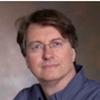
\includegraphics[width=1.0\columnwidth]{images/gregor.png}
  \caption{A demonstration in the scalability of PDF images.}
  \label{F:flow}
\end{figure}
\end{verbatim}

Which results in the following:
\begin{quote}
In Figure~\ref{F:flow} we show a black and white graph about ... .

\begin{figure}[htb]
  \includegraphics[width=1.0\columnwidth]{images/i523-overview.pdf}
  \caption{A demonstration in the scalability of PDF images.}
  \label{F:flow}
\end{figure}
\end{quote}

Note that las17graph must be a label of a valid bibtex entry. This is
needed if you have copied the image from elsewhere to avoid plagiarism.
However, if you came up with the graph yourself than you do not need a
citation.

We recommend that you place in your paper drafts all images at the which
can be done with the endfloat package

This can be enabled if you include the following lines before begin
document command:

\begin{verbatim}
\usepackage{endfloat}
\renewcommand{\efloatseparator}{\mbox{}} 

\begin{document}
\end{verbatim}

\subsection{Tables}\label{tables}
\index{Latex!Elements!tables}

Latex tables are very similar to csv table. Thus you could with
appropriate manipulation create tables from csv tables and use tools
such as spreadsheet editors to manage your table. There are even
packages that allow you to import the contents of csv tables directly
into \LaTeX.

In many cases you simply can start with an online table generator such as

\URL{https://www.tablesgenerator.com/}

For some tables you may want to rescale the width with

\begin{verbatim}
\resizebox{\textwidth}{!}{%
   ... PUT YOUR TABLE HERE ....
}
\end{verbatim}

In other cases you may want to rotate the table which you can easily
google for. In all cases use as figures, tables need to be in the
\verb|table| float environment. In contrast to figures captions are on
the top. All tables must be referred to by \verb|ref|. For more
information in directly including csv tables see 

\URL{http://mirror.utexas.edu/ctan/macros/latex/contrib/csvsimple/csvsimple.pdf}

However the format is very easy and can in most cases directly be
included in latex as shown in Table~\ref{T:elements}.

\begin{verbatim}
\begin{table}[htb]
\caption{Table with elements}\label{T:elements}
\bigskip
\begin{center}
\begin{tabular}{ c c c }
 column1  & column2  & column3 \\
\hline
\hline
 element1 & element2 & element3 \\ 
 element4 & element5 & element6 \\  
 element7 & element8 & element9 \\
\hline
\end{tabular}
\end{center}
\end{table}
\end{verbatim}

\begin{table}[htb]
\caption{Table with elements}\label{T:elements}
\bigskip
\begin{center}
\begin{tabular}{ c c c }
 column1  & column2  & column3 \\
\hline
\hline
 element1 & element2 & element3 \\ 
 element4 & element5 & element6 \\  
 element7 & element8 & element9 \\
\hline
\end{tabular}
\end{center}
\end{table}

\subsection{Labels}\label{labels}
\index{Latex!Elements!labels}

As we saw already for figures and tables it is recommended to use the
label and ref commands to refer to figure or table numbers. This applies
also to sections. Thus I can place a label after a section:

\begin{verbatim}
\section{Introduction}\label{S:introduction}
\end{verbatim}

and write elsewhere in the paper:

\begin{verbatim}
As we showcased in Section~\ref{S:introduction}
\end{verbatim}

Furthermore to conveniently distinguish sections tables and figures, we
use the prefix S T F followed by a colon for the label. This helps
organizing your paper in case you have many labels.

\subsection{Mathematics}\label{math}
\index{Latex!Elements!mathematics}

One of the strength of LaTeX thi the ability to write easily
sophisticated mathematical expressions on paper with high quality. A
good online resource is provided by the following online resource from
which we have copied some examples:

\begin{itemize}

\item
  \url{https://en.wikibooks.org/wiki/LaTeX/Mathematics}
\end{itemize}

To activate them use 

\begin{verbatim}
\usepackage{amsmath}
\end{verbatim}

at the beginning of the document after the document class

Exponents are using the \^{} character:

\begin{tcblisting}{colback=blue!5!white,colframe=gray!50!blue,listing side text,
  title=exponents,fonttitle=\bfseries}
$(a+b)^2 = a^2 + 2ab + b^{c+2}$
\end{tcblisting} 

Greek letters are referred to by their name proceeded by the slash:

\begin{tcblisting}{colback=blue!5!white,colframe=gray!50!blue,listing side text,
  title=greek,fonttitle=\bfseries}
$ \alpha \beta \gamma \Gamma \pi \Pi \phi $
\end{tcblisting}


Limits can be written as follows:

\begin{tcblisting}{colback=blue!5!white,colframe=gray!50!blue,listing side text,  title=limits,fonttitle=\bfseries}
$ \lim_{x \to \infty} \exp(-x) = 0 $
\end{tcblisting}

Fractions are indicated by the frac command, and binomials by binom:

\begin{tcblisting}{colback=blue!5!white,colframe=gray!50!blue,listing side text,  title=fraction,fonttitle=\bfseries}
$ \frac{n!}{k!(n-k)!} = \binom{n}{k} $   
\end{tcblisting}

Matrices can be created as follows:

\begin{tcblisting}{colback=blue!5!white,colframe=gray!50!blue,listing side text,  title=matrix,fonttitle=\bfseries}
$ A_{m,n} = 
\begin{pmatrix}
  a_{1,1} & a_{1,2} & \cdots & a_{1,n} \\
  a_{2,1} & a_{2,2} & \cdots & a_{2,n} \\
  \vdots  & \vdots  & \ddots & \vdots  \\
  a_{m,1} & a_{m,2} & \cdots & a_{m,n} 
\end{pmatrix} $
\end{tcblisting}



\section{Advanced topics}

\subsection{ACM and IEEE Proceedings Format}\label{acm-proceedings-format}
\index{Latex!proceedings!acm}
\index{Latex!proceedings!ieee}

\begin{figure}[!h]
  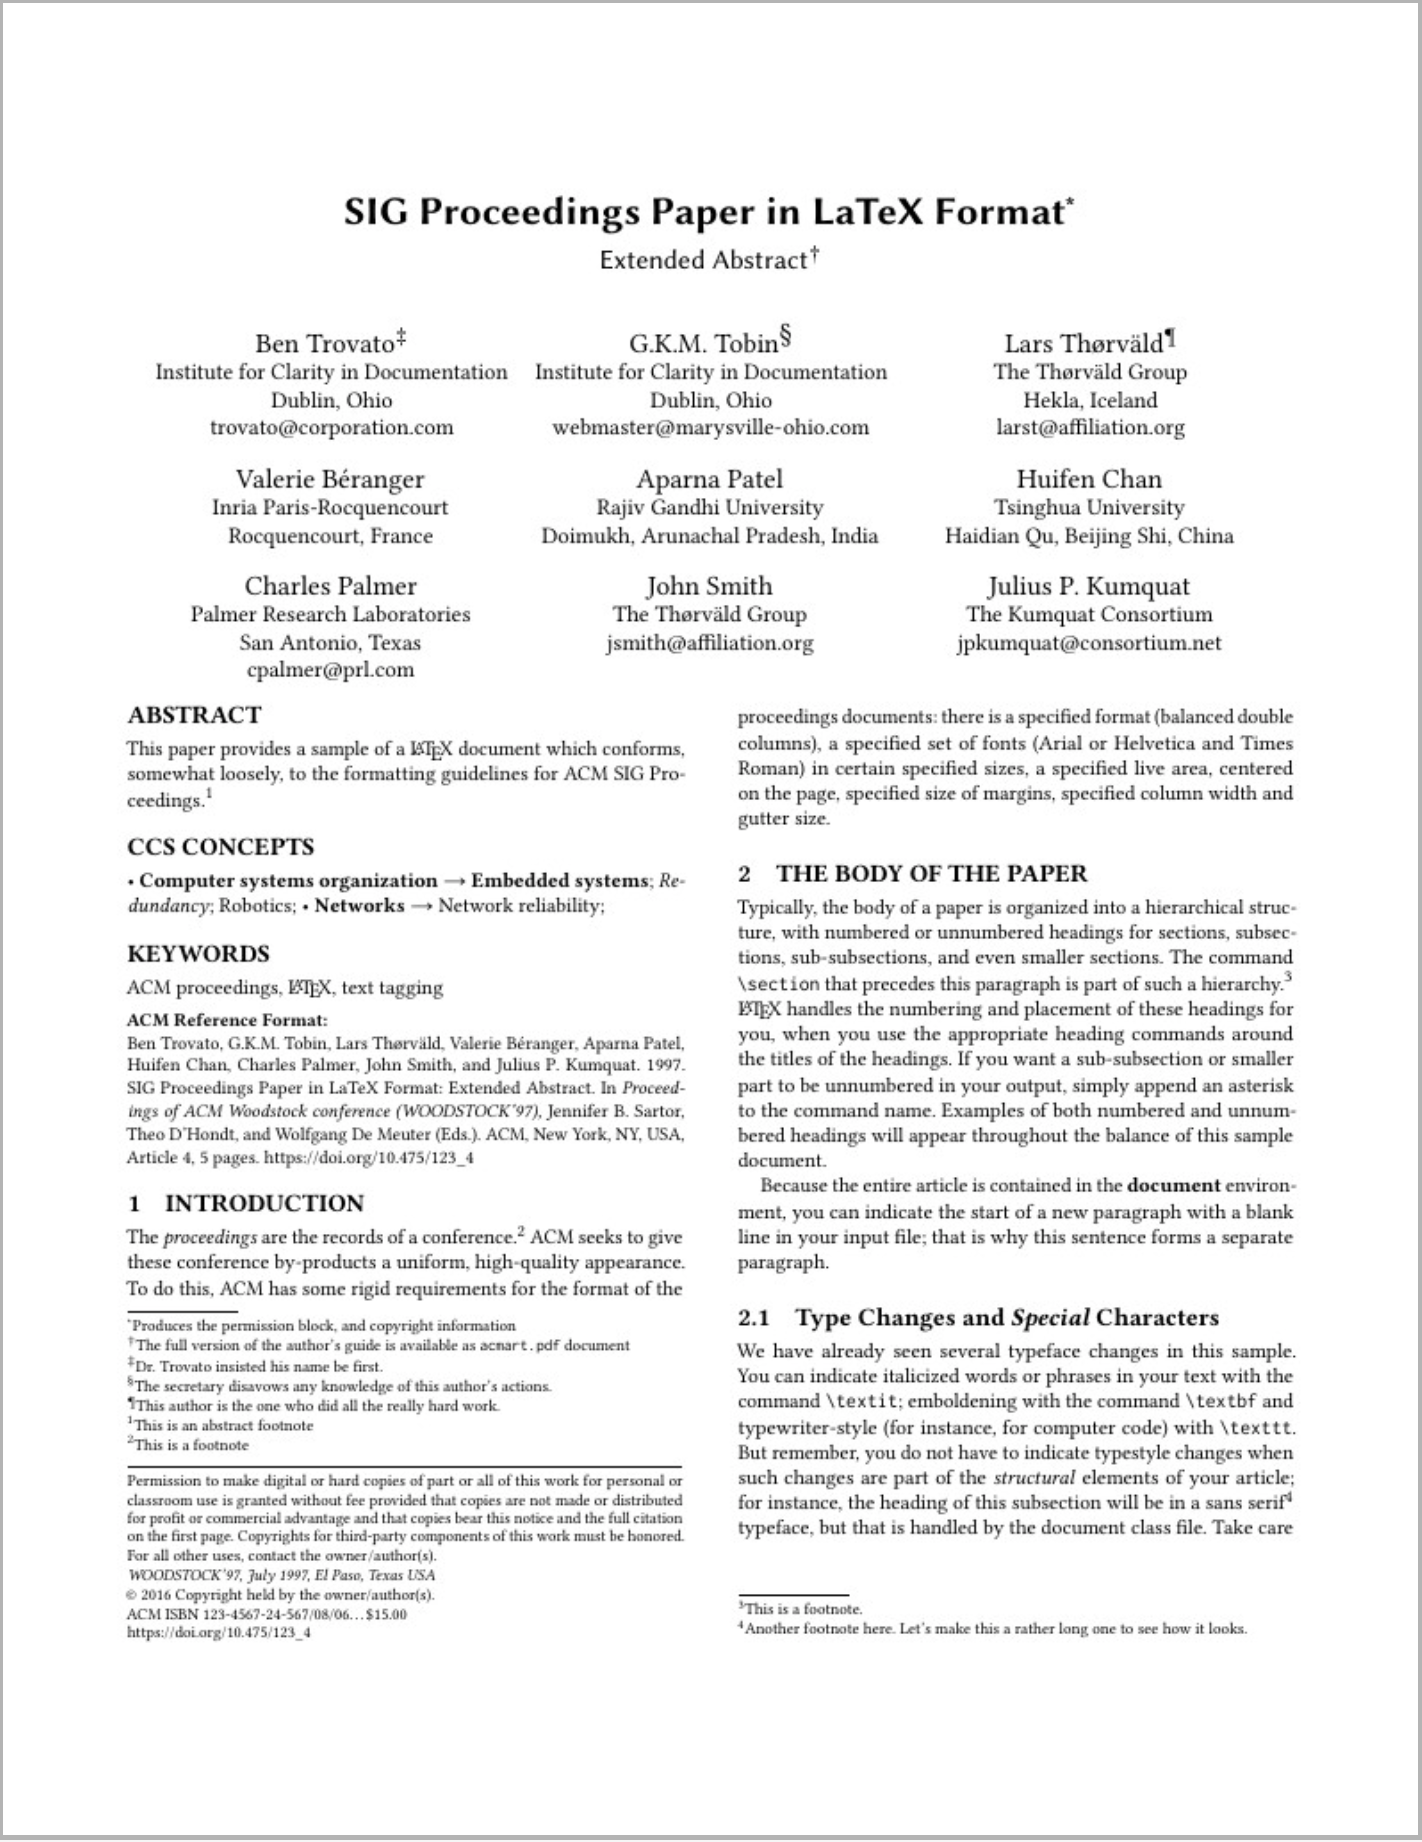
\includegraphics[width=6cm]{images/doc/acm.png}
  \hfill
  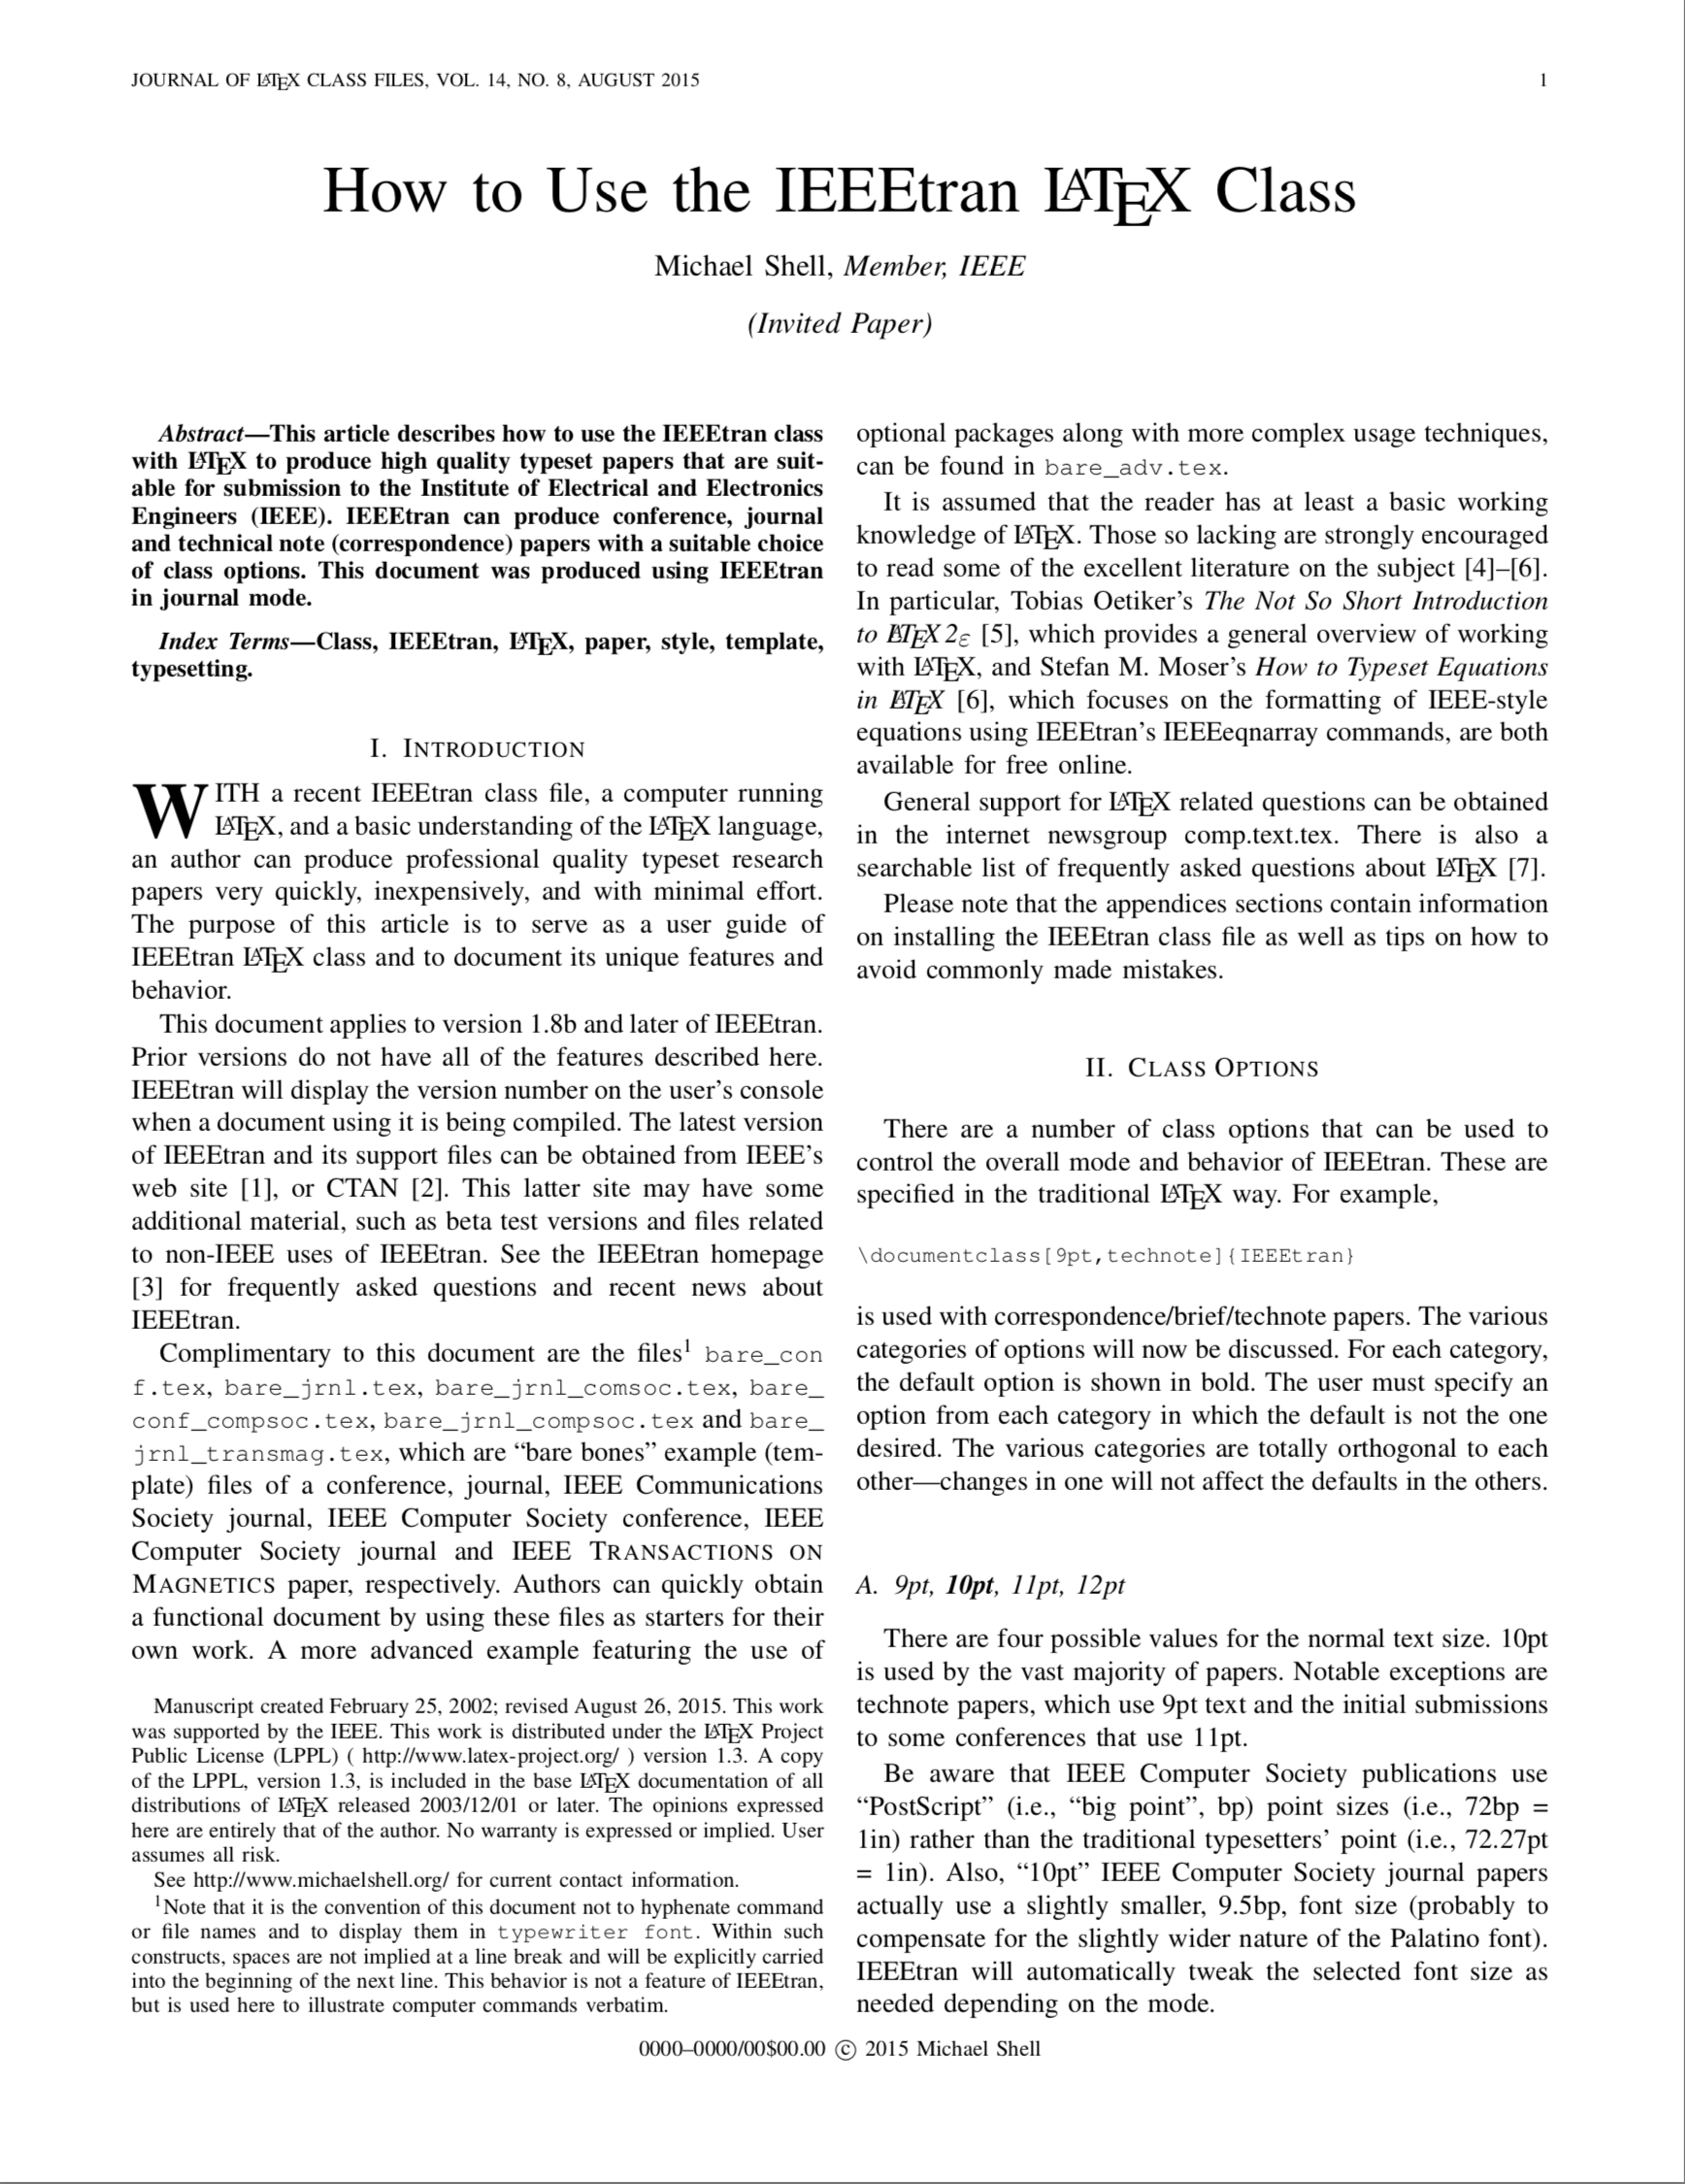
\includegraphics[width=6cm]{images/doc/ieee.png}
\caption{The look of the ACM and IEEE format templates}
\end{figure}

\begin{itemize}

\item
  \url{http://www.acm.org/publications/proceedings-template}
\item
  \url{https://www.ieee.org/conferences_events/conferences/publishing/templates.html}
\end{itemize}

\subsection{Generating and Managing Images}\label{generating-images}

To produce high quality images the programs PowerPoint and omnigraffle
on OSX are recommended. When using powerpoint please keep the image
ratio to 4x3 as they produce nice size graphics which you also can use
in your presentations. When using other rations they may not fit in
presentations and thus you may increase unnecessarily your work. We do
not recommend vizio as it is not universally available and produces
images that in case you have to present them in a slide presentation
does not easily reformat if you do not use 4x3 aspect ratio.

Naturally, graphics should be provided in SVG or PDF format so they can
scale well when we look at the final PDF. Including PNG, gif, or jpeg
files often do not result in the necessary resolution or the files
become real big. For this reason we for example can also not recommend
tools such as tablaeu as they do not provide proper exports to high
quality publication formats. For interactive display such tool may be
good, but for publications it produces inferior formatted images.

We recommend that all images be stored into a folder called images in
the same directory where your \LaTeX~ main document resides.



\subsection{Colored Boxes}

The package \verb|tcolorbox| provides sophisticated support to include
color boxes. Together with the new environment we can create nice add
ons to for example include notes.

\URL{http://osl.ugr.es/CTAN/macros/latex/contrib/tcolorbox/tcolorbox.pdf}

We have provided in this document notes as follows


\begin{tcblisting}{colback=blue!5!white,colframe=gray!50!blue,listing side text,  title=Note,fonttitle=\bfseries}
\begin{NOTE}
This is a note
\end{NOTE}
\end{tcblisting}

\begin{tcblisting}{colback=blue!5!white,colframe=gray!50!blue,listing side text,  title=Warning,fonttitle=\bfseries}
\begin{WARNING}
This is a note
\end{WARNING}
\end{tcblisting}


\subsection{Slides}\label{slides}
\index{Latex!slides}

Slides are best produced with the seminar package:

\begin{verbatim}
\documentclass{seminar}

\begin{slide}

    Hello World on slide 1

\end{slide}

The text between slides is ignored

\begin{slide}

    Hello World on slide 2

\end{slide}
\end{verbatim}

However, in case you need to have a slide presentation we recommend you
use ppt. Just paste and copy content from your PDF or your LaTeX source
file into the ppt.



\subsection{LaTeX vs. X}\label{latex-vs.-x}

We will refrain from providing a detailed analysis on why we use LaTeX
in many cases versus other technologies. In general, we find that LaTeX:

\begin{itemize}

\item
  is incredibly stable
\item
  produces high-quality output
\item
  is platform independent
\item
  has lots of templates
\item
  has been around for many years so it works well
\item
  removes you from the pain of figure placements
\item
  focusses you on content rather tan the appearance of the paper
\item
  integrates well with code repositories such as git to write
  collaborative papers.
\item
  has superior bibliography integration
\item
  has a rich set of tools that make using LaTeX easier
\item
  authors do not play with layouts much so papers in a format are
  uniform
\end{itemize}

In case you need a graphical view to edit LaTeX or LateX exportable
files you also find AucTeX and Lyx.

\subsubsection{Word}\label{word}

Word is arguably available to many, but if you work on Linux you may be
out of luck. Also Word often focusses not on structure of the text but
on its appearance. Many students abuse Word and the documents in Word
become a pain to edit with multiple users. Recently Microsoft has
offered online services to collaborate on writing documents in groups
which work well. Integration with bibliography managers such as endnote
or Mendeley is possible.

However, we ran into issues whenever we use word:

\begin{itemize}

\item
  Word tends sometimes to crash for unknown reasons and we lost a lot of
  work
\item
  Word has some issues with the bibliography managers and tends to crash
  sometimes for unknown reasons.
\item
  Word is slow with integration to large bibliographies.
\item
  Figure placement in Word in some formats is a disaster and you will
  spend many hours to correct things just to find out that if you make
  small changes you have to spend additional many hours to get used to
  the new placement. We have not yet experienced a word version where we
  have not lost images. Maybe that has changed, so let us know
\end{itemize}

However, we highly recommend the collaborative editing features of Word
that work on a paragraph and not letter level. Thus saving is essential
so you do not block other people from editing the paragraph.

\subsubsection{Google Docs}\label{google-docs}

Unfortunately, many useful features got lost in the new google docs.
However, it is great to collaborate quickly online, share thoughts and
even write your latex documents together if you like (just copy your
work in a file offline and use latex to compile it ;-) )

The biggest issue we have with Google Docs is that it does not allow the
support of 2 column formats, that the bibliography integration is
non-existent and that paste and copy from web pages and images
encourages unintended plagiarism when collecting information without
annotations (LaTeX and Word are prone to this too, but we found from
experience that it tends to happen more with Google docs users.

\subsubsection{A Place for Each}\label{a-place-for-each}

When looking at the tools we find a place for each:

\begin{description}
\item[Google docs:]
Short meeting notes, small documents, quick online collaborations to
develop documents collaboratively at the same time.
\item[Word:]
Available to many, supports 2 column format, supports paragraph based
collaborative editing, Integrates with bibliography managers.
\item[LaTeX:]
Reduces failures, great offline editing, superior bibliography
management, superior image placement, runs everywhere. Great
collaborative editing with sharelatex, allows easy generation of
proceedings written by hundreds of people with shared index.
\item[The best choice for your class:]
LaTeX
\end{description}

\section{Editing}\label{editing}

\subsection{Emacs}\label{emacs}

The text editor emacs provides a great basis for editing TeX and LaTeX
documents. Both modes are supported. In addition there exists a color
highlight module enabling the color display of LaTeX and TeX commands.
On OSX aquaemacs and carbon emacs have build in support for LaTeX. Spell
checking is done with flyspell in emacs.

\subsubsection{Aquamacs}

Aquamacs is an editor based on GNU Emacs that runs on OSX and
integrates with the OSX desktop. This is for many the preferred editor
on OSX for \LaTeX.

\url{http://aquamacs.org}

\begin{figure}[!htb]
  \centering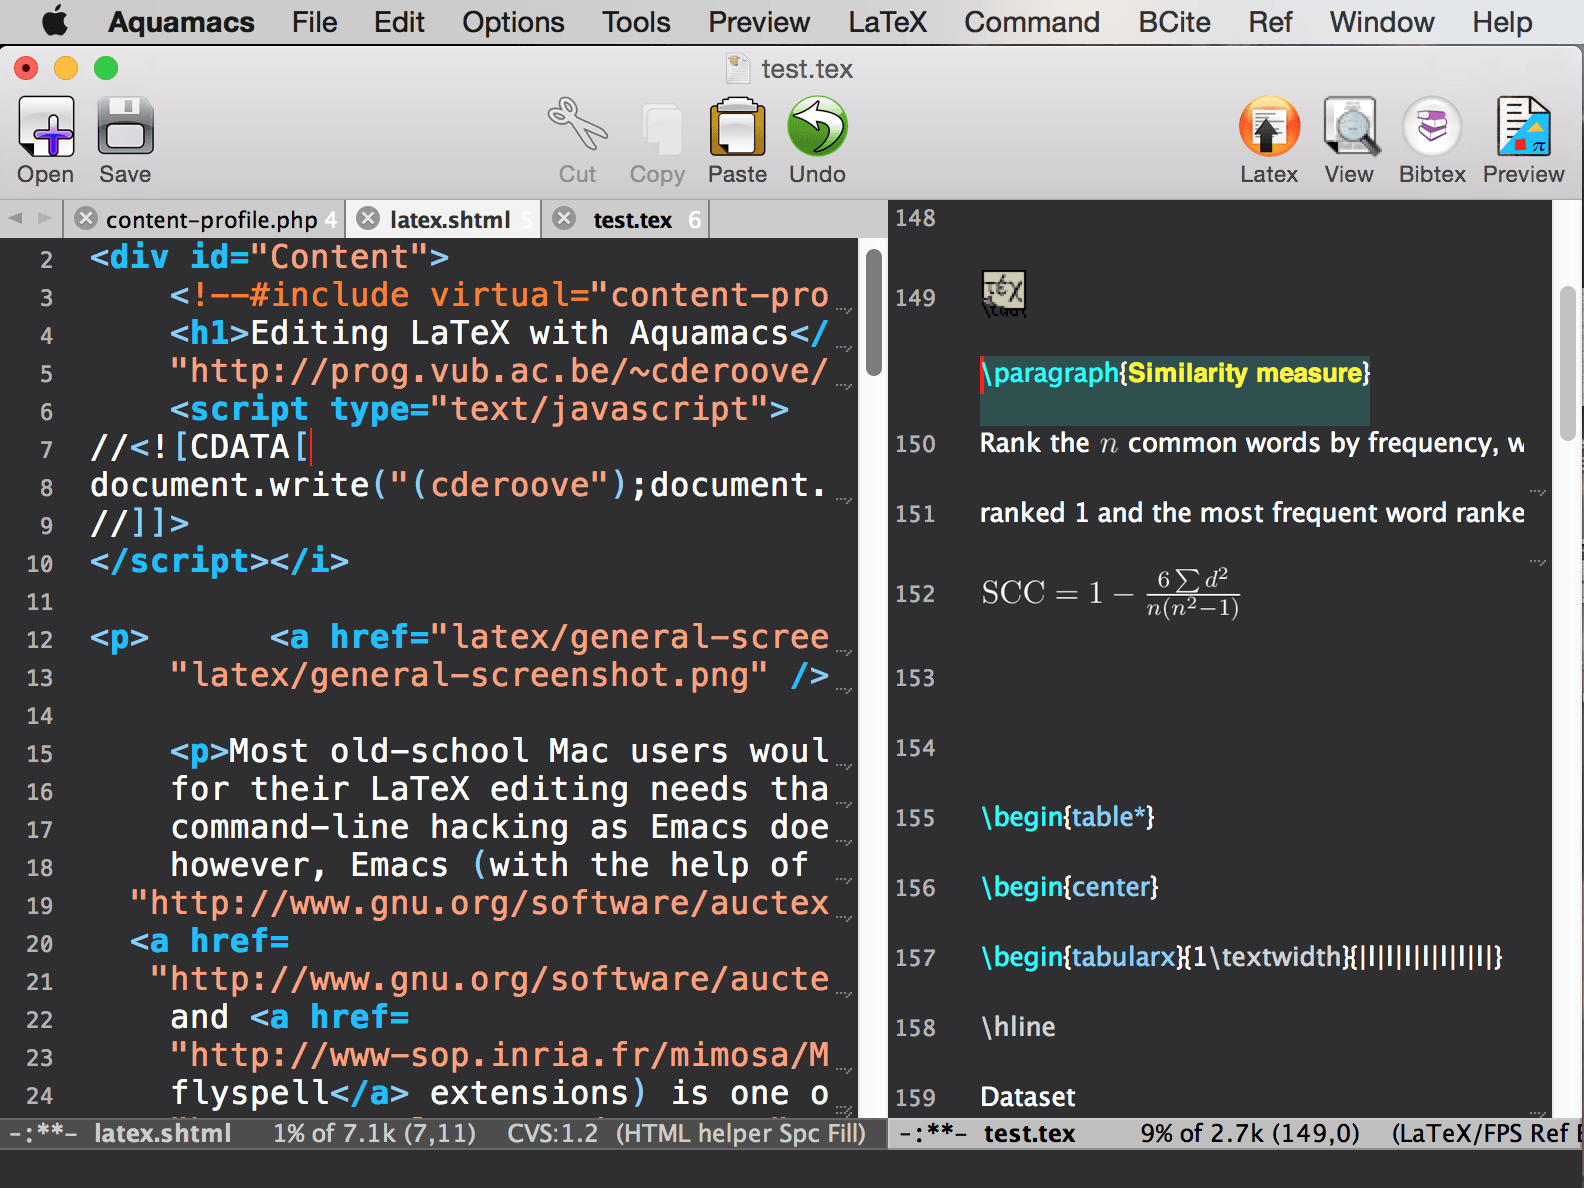
\includegraphics[width=8cm]{images/aquamacs.png}
  \caption{Aquamacs}
  \label{F:aquamacs}
\end{figure}


\subsection{Vi/Vim}\label{vivim}

Another popular editor is vi or vim. It is less feature rich but many
programmers ar using it. As it can edit ASCII text you can edit LaTeX.
With the LaTeX add-ons to vim, vim becomes similar powerful while
offering help and syntax highlighting for LaTeX as emacs does. (The
authors still prefer emacs)

\subsection{TeXshop}\label{texshop}

Other editors such as TeXshop are available which provide a more
integrated experience. However, we find them at times to stringent and
prefer editors such as emacs.

\subsection{LyX}\label{lyx}

We have made very good experiences with Lyx. You must assure that the
team you work with uses it consistently and that you all use the same
version.

\begin{figure}[!htb]
  \centering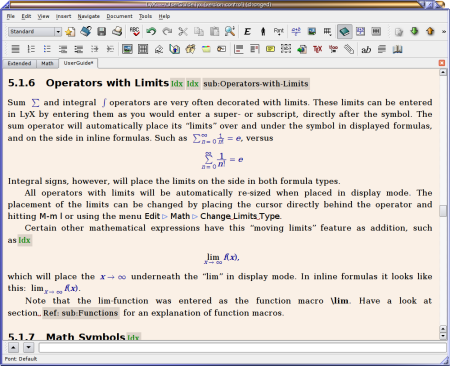
\includegraphics[width=8cm]{images/lyx.png}
  \caption{Lyx}
  \label{F:lyx}
\end{figure}

Using the ACM templates is documented here:

\begin{itemize}

\item
  \url{https://wiki.lyx.org/Examples/AcmSiggraph}
\end{itemize}

On OSX it is important that you have a new version of LaTeX and Lyx
installed. As it takes up quite some space, you ma want to delete older
versions. The new version of LyX comes with the acmsigplan template
included. However on OSX and other platforms the .cls file is not
included by default. However the above link clearly documents how to fix
this.

\subsection{WYSIWYG locally}\label{wysiwyg-locally}

We have found that editors such as Lyx and Auctex provide very good
WYSIWYG alike features. However, we found an even easier way while using
skim, a pdf previewer, in conjunction with emacs and latexmk. This can
be achieved while using the following command assuming your latex file
is called `report.tex`:

\begin{verbatim}
latexmk -pvc -view=pdf report
\end{verbatim}

This command will update your pdf previewer (make sure to use skim)
whenever you edit the file report.tex and save it. It will maintain via
skim the current position, thus you have a real great way of editing in
one window, while seeing the results in the other.

Skim can be found at: \url{http://skim-app.sourceforge.net/}

\subsection{Markdown and \LaTeX}
\index{Latex!markdown}

It may come as a surprise to many that one can actually write simple
LaTeX documents also in markdown Syntax or mix section written in
markdown while others are written in LaTeX. To do so all you ahve to
do is place the markdown text in a separate file. Let us call the file 
\verb|content.md| which has the following lines included in it:

\begin{verbatim}
# Section

* item a
* item b
\end{verbatim}

Obviously, we would have to convert this to LaTeX. Luckily there is a
very useful program called \textit{pandoc} that does this for you. YOu
could make the translation in the shell, but you could also make the
translation locally on your computer while allowing \LaTeX~ to start up
external programs. This is achieved with the \textit{write18} command and
allowing LaTeX explicitly to call external programs. Please inspect
the following latex file that includes a template on how to do
this. We assume the file is called markdown.tex for our example.

\begin{verbatim}
\documentclass{article}

\include{graphicx}
\newcommand{\tightlist}{}

\begin{document}
\immediate\write18{pandoc content.md -o content.tex}

\input{content}

\end{document}
\end{verbatim}

Now to generate the PDF we simply have to call the following command
that include the \textit{-shell-escape} flag to allow the execution of
write18 embedded commands:

\begin{verbatim}
pdflatex -shell-escape markdown-test
\end{verbatim}

The output will be \textit{markdown.pdf} with the content from the
markdown file translated. Doing this naturally allows you to write
large portions in markdown and automatically include them in your
LaTeX document. Hence, you can use editors such as Macdown to initially
work in semi WYSIWYG mode and do fairly straight forward
edition. Naturally the same can be done in RST. Naturally the most
elementary features are supported. For more sophisticated features,
please use LaTeX directly.


\subsection{Including RST into LaTeX}

content.rst:

\begin{verbatim}
Section
-------

* item a
* item b
\end{verbatim}

sample.tex:

\begin{verbatim}
\documentclass{article}

\include{graphicx}
\newcommand{\tightlist}{}

\begin{document}
\immediate\write18{pandoc content.rst -o content.tex}

\input{content}

\end{document}
\end{verbatim}


\subsection{pyCharm}

TODO: comment on how we can use pycharm for editing and what the
limitations are.

\subsection{MSWord}

it is possible to use Word.

be careful with 

\section{The LaTeX Cycle}\label{the-latex-cycle}
\index{Latex!cycle}

To create a PDF file from latex yo need to generate it following a
simple development and improvement cycle.

First, Create/edit ASCII source file with \texttt{file.tex} file:

\begin{verbatim}
emacs file.tex
\end{verbatim}

Create/edit bibliography file:

\begin{verbatim}
jabref refs.bib
\end{verbatim}

Create the PDF:

\begin{verbatim}
pdflatex file
bibtex file
pdflatex file
pdflatex file
\end{verbatim}

View the PDF:

\begin{verbatim}
open file
\end{verbatim}

It not only showcases you an example file in ACM 2 column format, but
also integrates with a bibliography. Furthermore, it provides a sample
Makefile that you can use to generate view and recompile, or even
autogenerate. A compilation would look like:

\begin{verbatim}
make
make view
\end{verbatim}

If however you want to do things on change in the tex file you can do
this automatically simply with:

\begin{verbatim}
make watch
\end{verbatim}

for make watch its best to use skim as pdf previewer


\section{Tips}\label{tips}

Including figures over two columns:

\begin{itemize}
\item
  \url{http://tex.stackexchange.com/questions/30985/displaying-a-wide-figure-in-a-two-column-document}
\item
  positioning figures with textwidth and columnwidth
  \url{https://www.sharelatex.com/learn/Positioning_images_and_tables}
\item
  An organization as the author. Assume the author is National Institute
  of Health and want to have the author show up, please do:

\begin{verbatim}
key= {National Institute of Health},
author= {{National Institute of Health}},
\end{verbatim}

  Please note the \{\{ \}\}
\item
  words containing `fi' or `ffi' showing blank places like below after
  recompiling it: find as nd efficiency as e ciency

  You copied from word or PDF ff which is actually not an ff, but a
  condensed character, change it to ff and ffi, you may find other such
  examples such as any non ASCII character. A degree is for example
  another common issue in data science.
\item
  do not use \textbar{} \& and other latex characters in bibtex
  references, instead use , and the word and
\item
  If you need to use \_ it is \_ but if you use urls leave them as is
\item
  We do recommend that you use sharelatex and jabref for writing papers.
  This is the easiest solution and beats in many cases MSWord as you can
  focus on writing and not on formatting.
\end{itemize}

\subsection{Colorful Output}

Instead of using pdflatex, you can also install \verb|pydflatex| that
provides a convenient wrapper and colorizes the output while
eliminating a lot of warnings that you may initially not want to deal
with. To install it please use:

\begin{verbatim}
pip install blessings
pip install -e "git+https://github.com/olivierverdier/pydflatex#egg=pydflatex"
\end{verbatim}

You can see the manual page with 

\begin{verbatim}
pydflatex --help

usage: usage: pydflatex [options] texfile1

Compile a tex file with pdflatex and make the auxiliary files invisible. Note
that the '.tex' extension may be omitted

positional arguments:
  tex path            path to tex file

optional arguments:
  -h, --help          show this help message and exit
  -o, --open          view the pdf file(s) in a pdf viewer.
  -k, --continue      continue on error
  -w, --with-warning  do not suppress common warnings
  -v, --verbose       Verbose output for debugging
  -p, --plain         No coloured output
  -x, --xetex         Use XeLaTeX engine
  -l, --log-parsing   Only parse log
  -t, --typesetting   Only typeset
\end{verbatim}

\subsection{latex2html}

\LaTeX~ can be exported to html with the the tool
\verb|latex2html|. It is available 

for Linux and OSX. More information can be found at

\URL{http://mirrors.ctan.org/support/latex2html/manual.pdf}

\URL{www.latex2html.org}

\begin{WARNING}
At this time the inastallation via brew install of latex2html is
broken. Instead one needs to conduct the insalation from source.

\begin{verbatim}
brew install latex2html
\end{verbatim}
\end{WARNING} 

The instalation from source can be conducted as follows

\begin{verbatim}
brew install libpng
wget https://github.com/latex2html/latex2html/archive/master.zip
uzip master.zip 
cd latex2html-master/
configure
make
make check
sudo make install
\end{verbatim}

\subsection{lachek}
\label{s:lacheck}
\index{lacheck}
\index{\LaTeX!lacheck}

Lacheck allows to find­ing common mistakes in \LaTeX~
documents. We recommend that you use it to check your latex files.

You can invoke it as follows

\begin{lstlisting}
lacheck filename.tex
\end{lstlisting}

More information can be found at

\URL{https://ctan.org/tex-archive/support/lacheck}

\subsection{chktex}
\label{s:chktex}
\index{chktex}
\index{\LaTeX!chktex}

LaTeX is a powerfull program to develop professional documents. In
some cases i is useful to check some semantics on the document. For
this reason you can use 

\begin{lstlisting}
chktex filename.tex
\end{lstlisting}

It will execute a number of filters and produce a check on them. You
can configure it to produce warnings and errors based on the error
type.

For a manual page use

\begin{lstlisting}
chktex --help
\end{lstlisting}

When using it some errors and wrnings can be ignored, while others
should be considerd. Supported featured mantiond on the Web page
include:
``
\begin{itemize}
          \item  Commands terminated with space. Ignores \verb|\tt|, etc.
          \item  Space in front of references instead of \verb|~|.
          \item  Forgetting to group parenthesis characters when
            sub-/superscripting.
          \item  Italic correction (\verb|\/|) mistakes (double, missing,
            unnecessary).
          \item  Parenthesis and environment matching.
          \item  Ellipsis detection; also checks whether to use \verb|\dots|,
            \verb|\cdots| or \verb|\ldots|.
          \item  Enforcement of normal space after abbreviation. Detects most
            abbreviations automagically.
          \item  Enforcement of end-of-sentence space when the last sentence
            ended with capital letter.
          \item  Math-mode on/off detection.
          \item  Quote checking, both wrong types (\verb|"|) and wrong direction.
          \item  Recommends splitting three quotes in a row.
          \item  Searching for user patterns.
          \item  Displays comments.
          \item  Space in front of \verb|\label| and similar commands.
          \item  Use of \verb|x| instead of \verb|$\times$| between numbers.
          \item  Multiple spaces in input which will be rendered as one space
            (or multiple spaces, where that is undesirable).
          \item  Warns about text which may be ignored.
          \item  Mathematical operators typeset as variables.
          \item  No space in front of/after parenthesis.
          \item  Demands a consistent quote style.
          \item  Punctuation inside inner math mode/outside display math mode.
          \item  Use of TeX primitives where LaTeX equivalents are available.
          \item  Space in front of footnotes.
          \item  Bogus characters following commands.
\end{itemize}
``

For more details see

\URL{http://baruch.ev-en.org/proj/chktex/}

\subsection{References}
\index{Latex!other documentation}

\begin{description}


\item[Latex Sheet:]    \url{https://wch.github.io/latexsheet/latexsheet.pdf}

\item[Latex Short:]    \url{http://tug.ctan.org/info/lshort/english/lshort.pdf}

\item[Wikibook:]       \url{https://en.wikibooks.org/wiki/LaTeX}
\item[Wikibook (PDF)]: \url{https://upload.wikimedia.org/wikipedia/commons/2/2d/LaTeX.pdf}

\item [Links to books:] \url{https://latexforhumans.wordpress.com/2008/10/11/the-best-guides-to-latex/}
\item [Links to books:] \url{https://www.latex-project.org/help/books/}
\item [LaTeX2e:]
  The
  \href{http://texdoc.net/texmf-dist/doc/latex/latex2e-help-texinfo/latex2e.pdf}{LaTeX
  Reference Manual} provides a good introduction to Latex.

\end{description}


\begin{itemize}

\item
  LaTeX Users and Reference Guide, by Leslie Lamport
  \url{https://www.amazon.com/LaTeX-Document-Preparation-System-2nd/dp/0201529831/ref=sr_1_2?s=books\&ie=UTF8\&qid=1507114870\&sr=1-2\&keywords=lamport}
\item
  LaTeX an Introduction, by Helmut Kopka
  \url{https://www.amazon.com/Guide-LaTeX-4th-Helmut-Kopka/dp/0321173856/ref=pd_lpo_sbs_14_t_0?_encoding=UTF8\&psc=1\&refRID=2BB4APDFEX34A4JM65ZB}
\item
  The LaTeX Companion, by Frank Mittelbach
  \url{https://www.amazon.com/LaTeX-Companion-Techniques-Computer-Typesetting/dp/0201362996}
\end{itemize}



\chapter{Managing Bibliographies}
\label{C:bibtex}

\FILENAME

\section{Integrating Bibliographies}
\label{S:bibliographies}
\index{Bibliography}
\index{bibtex}
\index{biber}

Bibliography management in \LaTeX\ is one of the many features that
motivate many researchers to make \LaTeX the tool of choice to write
academic papers. There are numerous bibliography styles available that
allow easy adaptation to differen journal and proceedings style. As
such, it includes styles for bibliographies formated in ACM and IEEE
style.

\subsection{biber}

\TODO{Describe use of biber instead of bibtex}

\subsection{bibtex}

This section assumes we use the standard bibtex program to integrate
citations into a \LaTeX\ paper.

An example to use the IEEE style for a paper includes to set
the style to IEEEtran before you add the reference:

\begin{verbatim}
\bibliographystyle{IEEEtran}
\bibliography{references.bib}
\end{verbatim}

To properly create PDF papers which using bibtex, we have to make sure
that all indexes, citations, references and labels are updated. This
is done with the help of the following commands assuming your file is
called \verb|file.tex|

\begin{verbatim}
pdflatex  file
bibtex file
pdflatex  file
pdflatex  file
\end{verbatim}


\begin{IU}
At IU you are required to use our template. which includes a Makefile
and either calls the above three commands or used latexmk
\end{IU}

The reason for the multiple execution of the latex program is to update
all cross-references correctly. In case you are not interested in
updating the library every time in the writing progress just postpone it
till the end. Missing citations are viewed as {[}?{]}.

Two programs stand out when managing bibliographies: emacs and jabref:

  \URL{http://www.jabref.org/}

Other programs such as Mendeley, Zotero, and even endnote integrate with
bibtex. However their support is limited, so we recommend that you just
use jabref as it is free and runs on all platforms.

\subsection{jabref}\label{jabref}

\TODO{Tyler: include cite for jabref, bibtex, biber at appropriate
  location in this section. Add them to the bib file.}

Practical experience with many generations of students shows that
\textit{jabref} is a very simple to use bibliography manager for LaTeX and
other systems. It can create a multitude of bibliography file formats
and allows upload in other online bibliography managers.

For information on how to install and use jabref please go to 
\url{http://www.jabref.org/}. There you will find the appropriate
download link.

We provide also a convenient video on how to use jabref and show
several methods on how to add entries easily to your bibliography database.

\video{Bibliography}{1:41}{jabref}{https://youtu.be/QVbifcLgMic}



\section{Entry types}

In this section we will explain how to find and properly generate
bibliographic entries. We are using bibtex for this as it is easy to
use and generates reasonable entries that can be included in
papers. What we like to achieve in this section is not to just show
you a final entry, but to document the process on how that entry was
derived. This will allow you to replicate or learn from the process to
apply to your own entries. As part of this we copy and paste
information found via Web searches.

We will address a number of important reference types which includes:

\begin{itemize}

\item
  wikipedia entries
\item
  github (see Section~\ref{s:e:source-code-references})
\item
  books
\item
  articles in a scientific journal (see Section~\ref{s:e:article-in-a-journal})
\item
  articles in a conference (see Section~\ref{s:e:article-in-a-conference-proceedings})
\item
  articles in magazines (non scientific)
\item
  blogs
\end{itemize}

\subsection{Source Code References}
\label{s:e:source-code-references}
\index{Bibtex!Source code}

Often, we need to cite a source code from a publicly hosted
repository. Such repositories are frequently used and include, for
example github, bitbucket, sourceforge, or your Universities code
repository as long as it is publicly reachable. As changes can occur on
these repositories, it is important that the date of access is listed in
the entry or even the release version of the source code.

Let us without bias chose a random source dode entry that has been
contributed by a student as follows:

\begin{verbatim}
@Misc{gonzalez_2015,
  Title =  {Buildstep},
  Author =     {Gonzalez, Jose and Lindsay, Jeff},
  HowPublished = {Web Page},
  Month =  {Jul},
  Note =   {Accessed: 2017-1-24},
  Year =   2015,
  Key =        {www-buildstep},
  Url =        {https://github.com/progrium/buildstep}
}
\end{verbatim}

Is this entry correct? Let us analyse. But first we need to undersrand
the semantics of the fields.

\subsubsection{What are the Different entry Types and Fields}

You see that the entry contains a number of fields. An extensive
explanation of these fields can be found at 

Please see \url{https://en.wikipedia.org/wiki/BibTeX}

We provide for this example a comprehensive discussions of the fields
used. For other examples we suggest you refer to the document to
identify what needs to be filled out.

\subsubsection{Entry type Misc}\label{s:e:entry-type-misc}
\index{Bibtex!Field!Misc}

First, it seems appropriate to use a \emph{@misc} entry. We correctly
identify this is a misc entry as it is online available. More recent
version of bibtex include also the type \emph{@online} for it. However,
in order to maintain compatibility to older formats we chose simply Misc
here and if we really would need to we could replace it easily.

\subsubsection{Label}\label{s:e:label}
\index{Bibtex!Field!Label}

Typically the bibliography label should contain 3 letters from an
author name, short year and the short name of the publication to
provide maximum information regarding the publication. However in this
case the project is hosted on github, so creating the label based on
just the github location seems more logical. Thus our label that we
propose is given by 

\verb|github-progrium-buildstep|


Under no circumstances should you use underscores as they can have unintended
consequences in programs we use to create papers for our classes. Just
use a minus sign instead. As it is hosted on github we also want the
githubname and the projectname. As you can see we just derived it from
the URL.

\begin{IU}
When managing bibliography entries with large numbers of collaborators
it is advisable that all bibliography labels be initially be prefixed
with an id for the collaborator. In our case we use the HID. Thus in
our case we will have the following label.

\verb|hid-sp18-000-github-progrium-buildstep|

\end{IU}


\subsubsection{Author}\label{s:e:author}
\index{Bibtex!Field!Author}

Normally we can write in the author fiels the names of the authors
separated by the work and. IT is important tu use the word \verb|and|
but not use a comma. However, this only works if the lastname does not
contain a space in it. In order to avoid confusing the system, we
recommend therefore to write all names in the form
\verb|Lastname, Firstname Middle Initials|

Thus we find in our example

\verb|  Author =     {Gonzalez, Jose and Lindsay, Jeff},|

\begin{WARNING}
Please note the word and between authors. and not a comma, commas are
only used to distinguish between lastname and firstname.
\end{WARNING}


\subsubsection{Key}\label{s:e:key}
\index{Bibtex!Field!Key}

In this case the key field can be removed as the entry has an author
field entry. If there was no author field, we use the key to specify
the alphabetical ordering based on the specified key. Note that a key is
not the label. In fact in our original entry the key field was wrongly
used and the student did not understand that the key is used for
sorting.

\subsubsection{Howpublished}\label{s:e:howpublished}
\index{Bibtex!Field!Howpublished}

Since the source is a github project repository, the howpublished field
shall hold the value \verb|{Code Repository}|. If the
url specified was a normal webpage, the \verb|{Web Page}| entry would be
valid.

\subsubsection{Month}\label{s:e:month}
\index{Bibtex!Field!Month}

To allow internationalization of the month we use the first 3 letters
in the english language for the month. Thus it is 
\verb|month = jul|. Note that there are no brackets around the month.

\subsubsection{Owner}\label{s:e:owner}
\index{Bibtex!Field!Owner}

In class we introduced the convention to put the student HID in it. If
multiple students contributed, add them with space separation.

\subsubsection{Accessed}\label{s:e:accessed}
\index{Bibtex!Field!Accessed}

As some styles do not support the accessed field, we simply include it in
the note field. This is absolutely essential as code can change and when
we read the code we looked at a particular snapshot in time. In addition
it is often necessary to record the actual version of the code or the branch.
Typically for github entries, it is best to just use the month and
year field as some styles check for it.

\subsubsection{Final Entry}

Filling out as many fields as possible with information for this entry
we get:

\begin{verbatim}
@Misc{github-progrium-buildstep,
  Title =  {Buildstep},
  Author =     {Jose Gonzalez and Jeff Lindsay},
  HowPublished = {Code Repository},
  Year =   {2015},
  Month =  jul,
  Note =   {Accessed: 2017-1-24, master branch},
  Url =    {https://github.com/progrium/buildstep},
  Owner =  {S17-IO-3025},
}
\end{verbatim}

We are using the release date in the year and month field as this
project uses this for organizing releases. However, other project may
have release versions so you would have in addition to using the data
also to include the version in the note field such as:

\begin{verbatim}
Note =     {Version: 1.2.3, Accessed: 2017-1-24},
\end{verbatim}


\subsection{Pedigree}

Often it is advantageous to document the pedigree of the bibtex
entries. Eg, how did you derive the final entry? To do so you can
simply add a field such as \verb|bibsource| and include in it all
links you used to gather the final entry. However, we believe that the
effort to curate an entry is sufficient to manage your own
bibliography which you should freely distribute and constitute an own
contribution. 

\subsection{Article in a Journal}
\label{s:e:article-in-a-journal}
\index{Bibtex!Article}

Many online bibtex entries that you will find are wrong or
incomplete. Often you may find via google a bibtex entry that may need
some more research. Let us assume your first google query returns a
publication and you cite it such as this:

\begin{verbatim}
@Unpublished{unpublished-google-sawzall,
    Title = {{Interpreting the Data: Parallel Analysis with Sawzall}},
    Author = {{Rob Pike, Sean Dorward, Robert Griesemer, Sean Quinlan}},
    Note = {accessed 2017-01-28},
    Month = {October},
    Year = {2005},
    Owner = {for the purpose of this discussion removed},
    Timestamp = {2017.01.31}
}
\end{verbatim}

Could we improve this entry to achieve your best? We observe:

\begin{enumerate}
\item
  The author field has a wrong entry as the , is to be replaced by an
  and.
\item
  The author field has authors and thus must not have a \{\{ \}\}
\item
  The url is missing, as the simple google search actually finds a PDF
  document.
\end{enumerate}

Let us investigate a bit more while searching for the title. We find

\begin{enumerate}
\def\labelenumi{\Alph{enumi})}
\item
  \url{https://www.google.com/url?sa=t\&rct=j\&q}=\&esrc=s\&source=web\&cd=1\&ved=0ahUKEwj\_ytSA-PDRAhUH8IMKHaomC-oQFggaMAA\&url=https\%3A\%2F\%2Fresearch.google.com\%2Farchive\%2Fsawzall-sciprog.pdf\&usg=AFQjCNHSSfKBwbxVAVPQ0td4rTjitKucpA\&sig2=vbiVzi36B3gGFjIzlUKBDA\&bvm=bv.146073913,d.amc
\item
  \url{https://research.google.com/pubs/pub61.html}
\item
  \url{http://dl.acm.org/citation.cfm?id=1239658}
\end{enumerate}

Let us look at A)

As you can see from the url this is actually some redirection to a google
web page which probably is replaced by B as its from google research. So
let us look at B)

Now when you look at the link we find the url
\url{https://research.google.com/archive/sawzall-sciprog.pdf} which
redirects you to the PDF paper.

When we go to B) we find surprisingly a bibtex entry as follows:

\begin{verbatim}
@article{61,
  title = {Interpreting the Data: Parallel Analysis with Sawzall},
  author = {Rob Pike and Sean Dorward and Robert Griesemer and Sean Quinlan},
  year = 2005,
  URL = {https://research.google.com/archive/sawzall.html},
  journal = {Scientific Programming Journal},
  pages = {277--298},
  volume = {13}
}
\end{verbatim}

Now we could say let us be satisfied, but C) seems to be even more
interesting as its from a major publisher. So lats just make sure we
look at C)

If you go to C, you find under the colored box entitled Tools and
Resources a link called \textbf{bibtex}. Thus it seems a good idea to
click on it. This will give you:

\begin{verbatim}
@article{Pike:2005:IDP:1239655.1239658,
    author = {Pike, Rob and Dorward, Sean and Griesemer, Robert and Quinlan, Sean},
    title = {Interpreting the Data: Parallel Analysis with Sawzall},
    journal = {Sci. Program.},
    issue_date = {October 2005},
    volume = {13},
    number = {4},
    month = oct,
    year = {2005},
    issn = {1058-9244},
    pages = {277--298},
    numpages = {22},
    url = {http://dx.doi.org/10.1155/2005/962135},
    doi = {10.1155/2005/962135},
    acmid = {1239658},
    publisher = {IOS Press},
    address = {Amsterdam, The Netherlands, The Netherlands},
}
\end{verbatim}

Now we seem to be at a position to combine our search result as neither
entry is sufficient. As the doi number properly specifies a paper (look
up what a doi is) we can replace the url with one that we find online,
such as the one we found in A) Next we see that all field sin B are
already covered in C, so we take C) and add the url. Now as the label is
great and uniform for ACM, but for us a bit less convenient as its
difficult to remember, we just change it while for example using
authors, title, and year information. let us also make sure to do mostly
lowercase in the label just as a convention. Thus our entry looks like:

\begin{verbatim}
@article{pike05swazall,
    author = {Pike, Rob and Dorward, Sean and Griesemer, Robert and Quinlan, Sean},
    title = {Interpreting the Data: Parallel Analysis with Sawzall},
    journal = {Sci. Program.},
    issue_date = {October 2005},
    volume = {13},
    number = {4},
    month = oct,
    year = {2005},
    issn = {1058-9244},
    pages = {277--298},
    numpages = {22},
    url = {https://research.google.com/archive/sawzall-sciprog.pdf},
    doi = {10.1155/2005/962135},
    acmid = {1239658},
    publisher = {IOS Press},
    address = {Amsterdam, The Netherlands, The Netherlands},
}
\end{verbatim}

As you can see properly specifying a reference takes multiple google
queries and merging of the results you find from various returns. As
you still have time to correct things I advise that you check your
references and correct them. If the original reference would have been
graded it would have been graded with a ``fail'' instead of a ``pass''.

Naturally you need to judge if you can integrate the URL or not, often
papers exist in a prepublication and you must make sure to cite the
version you used. IN fact if you have the prepublicAtion, you should
obtain the final manuscript as it could contain significant
corrections to the previous draft. In other cases the prepublication
may just be fine and you could for your own references keep the
url. FOr the final publication you probably want to make sure that the
doi is used. FOr the collection of your references, adding the url
could be useful.

\subsection{Article in a Conference Proceedings}
\label{s:e:article-in-a-conference-proceedings}
\index{Bibtex!InProceedings}

Now let us look at another obvious example that needs improvement:

\begin{verbatim}
@InProceedings{wettinger-any2api,
  Title      = {Any2API - Automated APIfication},
  Author     = {Wettinger, Johannes and
                Uwe Breitenb{\"u}cher
                and Frank Leymann},
  Booktitle  = {Proceedings of the 5th International
                Conference on Cloud Computing and
                Services Science},
  Year       = {2015},
  Pages      = {475­486},
  Publisher  = {SciTePress},
  ISSN       = {2326-7550},
  Owner      = {S17-IO-3005},
  Url        = {https://pdfs.semanticscholar.org/1cd4/4b87be8cf68ea5c4c642d38678a7b40a86de.pdf}
}
\end{verbatim}

As you can see this entry seems to define all required fields, so we
could be tempted to stop here. But its good to double check. Let us do
some queries against ACM and google scholar. Let us just type in the
title, and if this is in a proceedings they should return hopefully a
predefined bibtex record for us.

Let us query:

\begin{verbatim}
google: googlescholar Any2API Automated APIfication
\end{verbatim}

We get:

\begin{itemize}

\item
  \url{https://scholar.google.de/citations?view_op=view_citation\&hl=en\&user=j6lIXt0AAAAJ\&citation_for_view=j6lIXt0AAAAJ:8k81kl-MbHgC}
\end{itemize}

On that page we see
\href{https://scholar.google.com/scholar_lookup?title=Automated+drug+dispensing+system+reduces+medication+errors+in+an+intensive+care+setting\&author=Chapuis\&publication_year=2010\#}{Cite}

So we find a PDF at
\url{https://pdfs.semanticscholar.org/1cd4/4b87be8cf68ea5c4c642d38678a7b40a86de.pdf}

Let us click on this and the document includes a bibtex entry such as:

\begin{verbatim}
@inproceedings{Wettinger2015, 
  author= {Johannes Wettinger and Uwe Breitenb{\"u}cher and Frank
       Leymann},
  title = {Any2API - Automated APIfication},
  booktitle = {Proceedings of the 5th International Conference on Cloud
       Computing and Service Science (CLOSER)},
  year = {2015},
  pages = {475--486},
  publisher = {SciTePress}
} 
\end{verbatim}

Now let us add the URL and owner:

\begin{verbatim}
@inproceedings{Wettinger2015, 
  author= {Johannes Wettinger and Uwe Breitenb{\"u}cher and Frank
       Leymann},
  title = {Any2API - Automated APIfication},
  booktitle = {Proceedings of the 5th International Conference on Cloud
       Computing and Service Science (CLOSER)},
  year = {2015},
  pages = {475--486},
  publisher = {SciTePress},
  url ={https://pdfs.semanticscholar.org/1cd4/4b87be8cf68ea5c4c642d38678a7b40a86de.pdf},
  owner = {S17-IO-3005},
} 
\end{verbatim}

Should we be satisfied? No, even our original information we gathered
provided more information. So let us continue. Let us issue additional
google searches with ACM or IEEE and the title. When doing the IEEE in the
example we find an entry called

\href{http://dblp.uni-trier.de\%2Fpers\%2Fl\%2FLeymann\%3AFrank\&usg=AFQjCNHCu-66qxWH0zRlPLr4DA8jIo5V-g\&sig2=1vYdnGOEiMcLBEMpbeBA7g}{dlp:
Frank Leyman}

Let us look at it and we find two entries:

\begin{verbatim}
@inproceedings{DBLP:conf/closer/WettingerBL15,
  author    = {Johannes Wettinger and
       Uwe Breitenb{\"{u}}cher and
       Frank Leymann},
  title     = {{ANY2API} - Automated APIfication - Generating APIs for Executables
       to Ease their Integration and Orchestration for Cloud Application
       Deployment Automation},
  booktitle = {{CLOSER} 2015 - Proceedings of the 5th International Conference on
       Cloud Computing and Services Science, Lisbon, Portugal, 20-22 May,
       2015.},
  pages     = {475--486},
  year      = {2015},
  crossref  = {DBLP:conf/closer/2015},
  url       = {http://dx.doi.org/10.5220/0005472704750486},
  doi       = {10.5220/0005472704750486},
  timestamp = {Tue, 04 Aug 2015 09:28:21 +0200},
  biburl    = {http://dblp.uni-trier.de/rec/bib/conf/closer/WettingerBL15},
  bibsource = {dblp computer science bibliography, http://dblp.org}
}

@proceedings{DBLP:conf/closer/2015,
  editor    = {Markus Helfert and
       Donald Ferguson and
       V{\'{\i}}ctor M{\'{e}}ndez Mu{\-{n}}oz},
  title     = {{CLOSER 2015 - Proceedings of the 5th International Conference on
       Cloud Computing and Services Science, Lisbon, Portugal, 20-22 May,
       2015}},
  publisher = {SciTePress},
  year      = {2015},
  isbn      = {978-989-758-104-5},
  timestamp = {Tue, 04 Aug 2015 09:17:34 +0200},
  biburl    = {http://dblp.uni-trier.de/rec/bib/conf/closer/2015},
  bibsource = {dblp computer science bibliography, http://dblp.org}
}
\end{verbatim}

So let us look at the entry and see how to get a better one for our
purpose and combine them. When using jabref, you see optional and
required fields, we want to add as many as possible, regardless if
optional or required, so Let us do that (We write it here in ASCII as it
is easier to document and can also be done in emacs:

\begin{verbatim}
@InProceedings{,
  author =   {},
  title =    {},
  OPTcrossref =  {},
  OPTkey =   {},
  OPTbooktitle = {},
  OPTyear =      {},
  OPTeditor =    {},
  OPTvolume =    {},
  OPTnumber =    {},
  OPTseries =    {},
  OPTpages =     {},
  OPTmonth =     {},
  OPTaddress =   {},
  OPTorganization = {},
  OPTpublisher = {},
  OPTnote =      {},
  OPTannote =    {},
  url = {}
}
\end{verbatim}

Now we copy and fill out the \textbf{form} from our various searches:

\begin{verbatim}
@InProceedings{Wettinger2015any2api,    
  author    = {Johannes Wettinger and
     Uwe Breitenb{\"{u}}cher and
     Frank Leymann},
  title     = {{ANY2API - Automated APIfication - Generating APIs for Executables
     to Ease their Integration and Orchestration for Cloud Application
     Deployment Automation}},
  booktitle = {{CLOSER 2015 - Proceedings of the 5th International Conference on
       Cloud Computing and Services Science}},
  year =     {2015},
  editor    = {Markus Helfert and
       Donald Ferguson and
       V{\'{\i}}ctor M{\'{e}}ndez Mu{\-{n}}oz},
  publisher = {SciTePress},
  isbn      = {978-989-758-104-5},
  pages = {475--486},
  month = {20-22 May},
  address =      {Lisbon, Portugal},
  doi       = {10.5220/0005472704750486},
  url ={https://pdfs.semanticscholar.org/1cd4/4b87be8cf68ea5c4c642d38678a7b40a86de.pdf},
  owner = {S17-IO-3005},
}
\end{verbatim}


For the rest of the section we provide just some simple examples.

\subsection{InProceedings}\label{s:e:inproceedings}
\index{Bibtex!InProceedings}

Please fill out

\begin{verbatim}
@InProceedings{,
  author =       {},
  title =        {},
  OPTcrossref =  {},
  OPTkey =       {},
  OPTbooktitle = {},
  OPTyear =      {},
  OPTeditor =    {},
  OPTvolume =    {},
  OPTnumber =    {},
  OPTseries =    {},
  OPTpages =     {},
  OPTmonth =     {},
  OPTaddress =   {},
  OPTorganization = {},
  OPTpublisher = {},
  OPTnote =      {},
  OPTannote =    {},
  url = {}
}
\end{verbatim}

\begin{verbatim}
@inproceedings{vonLaszewski15tas,
  author =     {DeLeon, Robert L. and Furlani, Thomas R. and Gallo,
                  Steven M. and White, Joseph P. and Jones, Matthew
                  D. and Patra, Abani and Innus, Martins and Yearke,
                  Thomas and Palmer, Jeffrey T. and Sperhac, Jeanette
                  M. and Rathsam, Ryan and Simakov, Nikolay and von
                  Laszewski, Gregor and Wang, Fugang},
  title =  {{TAS View of XSEDE Users and Usage}},
  booktitle =  {Proceedings of the 2015 XSEDE Conference: Scientific
                  Advancements Enabled by Enhanced
                  Cyberinfrastructure},
  series =     {XSEDE '15},
  year =   2015,
  isbn =   {978-1-4503-3720-5},
  location =   {St. Louis, Missouri},
  pages =  {21:1--21:8},
  articleno =  21,
  numpages =   8,
  url =        {http://doi.acm.org/10.1145/2792745.2792766},
  doi =        {10.1145/2792745.2792766},
  acmid =  2792766,
  publisher =  {ACM},
  address =    {New York, NY, USA},
  keywords =   {HPC, SUPReMM, TAS, XDMoD, XSEDE usage, XSEDE users},
}
\end{verbatim}

\subsection{TechReport}\label{s:e:techreport}
\index{Bibtex!TechReport}

Please fill out

\begin{verbatim}
@TechReport{,
  author =       {},
  title =        {},
  institution =  {},
  year =         {},
  OPTkey =       {},
  OPTtype =      {},
  OPTnumber =    {},
  OPTaddress =   {},
  OPTmonth =     {},
  OPTnote =      {},
  OPTannote =    {},
  url = {}    
}
\end{verbatim}

\begin{verbatim}
@TechReport{las05exp,
  title =  {{The Java CoG Kit Experiment Manager}},
  Author =     {von Laszewski, Gregor},
  Institution =    {Argonne National Laboratory},
  Year =   2005,
  Month =  jun,
  Number =     {P1259},
  url = {https://laszewski.github.io/papers/vonLaszewski-exp.pdf}
}
\end{verbatim}

\subsection{Article}
\index{Bibtex!Article}

Please fill out

\begin{verbatim}
@Article{,
  author =       {},
  title =        {},
  journal =      {},
  year =         {},
  OPTkey =       {},
  OPTvolume =    {},
  OPTnumber =    {},
  OPTpages =     {},
  OPTmonth =     {},
  OPTnote =      {},
  OPTannote =    {},,
  url = {}
}
\end{verbatim}

\begin{verbatim}
@Article{las05gridhistory,
  title =  {{The Grid-Idea and Its Evolution}},
  author =     {von Laszewski, Gregor},
  journal =    {Journal of Information Technology},
  year =   2005,
  month =  jun,
  number =     6,
  pages =  {319-329},
  volume =     47,
  doi =        {10.1524/itit.2005.47.6.319},
  url = {https://laszewski.github.io/papers/vonLaszewski-grid-idea.pdf}
}
\end{verbatim}

\subsection{Proceedings}\label{s:e:proceedings}
\index{Bibtex!Proceedings}

Please fill out

\begin{verbatim}
@Proceedings{,
  title =        {},
  year =         {},
  OPTkey =       {},
  OPTbooktitle = {},
  OPTeditor =    {},
  OPTvolume =    {},
  OPTnumber =    {},
  OPTseries =    {},
  OPTaddress =   {},
  OPTmonth =     {},
  OPTorganization = {},
  OPTpublisher = {},
  OPTnote =      {},
  OPTannote =    {},
  url = {}
}
\end{verbatim}

\begin{verbatim}
@Proceedings{las12fedcloud-proc,
  title =  {{FederatedClouds '12: Proceedings of the 2012
                  Workshop on Cloud Services, Federation, and the 8th
                  Open Cirrus Summit}},
  year =   2012,
  address =    {New York, NY, USA},
  editor =     {vonLaszewski, Gregor and Robert Grossman and Michael
                  Kozuchand Rick McGeerand Dejan Milojicic},
  publisher =  {ACM},
  iSBN =   {978-1-4503-1754-2},
  location =   {San Jose, California, USA},
  url =
                  {http://dl.acm.org/citation.cfm?id=2378975&picked=prox&cfid=389635474&cftoken=32712991}
}
\end{verbatim}

\subsection{Wikipedia Entry}\label{s:e:wikipedia-entry}
\index{Bibtex!Wikipedia Entry}

Please fill out

\begin{verbatim}
@Misc{,
  OPTkey =       {},
  OPTauthor =    {},
  OPTtitle =     {},
  OPThowpublished = {},
  OPTmonth =     {},
  OPTyear =      {},
  OPTnote =      {},
  OPTannote =    {},
  url = {}
}
\end{verbatim}

\begin{verbatim}
@Misc{www-ode-wikipedia,
  Title =  {Apache ODE},
  HowPublished = {Web Page},
  Note =   {Accessed: 2017-2-11},
  Key =        {Apache ODE},
  Url =        {https://en.wikipedia.org/wiki/Apache_ODE}
}
\end{verbatim}

\subsection{Blogs}\label{blogs}
\index{Bibtex!Blog}

Please fill out

\begin{verbatim}
@Misc{,
  OPTkey =       {},
  OPTauthor =    {},
  OPTtitle =     {},
  OPThowpublished = {},
  OPTmonth =     {},
  OPTyear =      {},
  OPTnote =      {},
  OPTannote =    {},
  OPTurl = {}
}
\end{verbatim}

\begin{verbatim}
@Misc{www-clarridge-discoproject-blog,
  title =  {Disco - A Powerful Erlang and Python Map/Reduce
                  Framework},
  uthor =  {Clarridge, Tait},
  howpublished = {Blog},
  month =  may,
  note =   {Accessed: 25-feb-2017},
  year =   2014,
  url =  {http://www.taitclarridge.com/techlog/2014/05/disco-a-powerful-erlang-and-python-mapreduce-framework.html}
}
\end{verbatim}

\subsection{Web Page}\label{s:e:web-page}
\index{Bibtex!Web Page}

Please fill out

\begin{verbatim}
@Misc{, 
  OPTkey =       {}, 
  OPTauthor =    {}, 
  OPTtitle =     {}, 
  OPThowpublished = {}, 
  OPTmonth =     {}, 
  OPTyear =      {}, 
  OPTnote =      {},
  OPTannote =    {},
  url = {}
}
\end{verbatim}

\begin{verbatim}
@Misc{www-cloudmesh-classes,
  OPTkey =       {},
  author =    {von Laszewski, Gregor},
  title =     {Cloudmesh Classes},
  howpublished = {Web Page},
  OPTmonth =     {},
  OPTyear =      {},
  OPTnote =      {},
  OPTannote =    {},
  url = {https://cloudmesh.github.io/classes/}
}
\end{verbatim}

\begin{verbatim}
@Misc{www-awslambda,
  title =  {AWS Lambda},
  author =     {{Amazon}},
  key =        {AWS Lambda},
  howpublished = {Web Page},
  url =        {https://aws.amazon.com/lambda/faqs/}
}
\end{verbatim}

\subsection{Book}\label{s:e:book}
\index{Bibtex!book}

Given the following entry. What is the proper entry for this book.
Provide rationale:

\begin{verbatim}
@Book{netty-book,
    Title = {Netty in Action},
    Author = {Maurer, Norman and Wolfthal, Marvin},
    Publisher = {Manning Publications},
    Year = {2016},
}
\end{verbatim}

To obtain the record of a book you can look at many information sources.
The can include:

\begin{itemize}

\item
  \url{https://www.manning.com/books/netty-in-action}
\item
  \url{https://www.amazon.com/Netty-Action-Norman-Maurer/dp/1617291471}
\item
  \url{http://www.barnesandnoble.com/w/netty-in-action-norman-maurer/1117342155?ean=9781617291470\#productInfoTabs}
\item
  \url{http://www.powells.com/book/netty-in-action-9781617291470/1-0}
\end{itemize}

Furthermore, we need to consider the entry of a book, we simply look it
up in emacs where we find the following but add the owner and the url
field:

\begin{verbatim}
@Book{,
  ALTauthor =      {},
  ALTeditor =      {},
  title =      {},
  publisher =      {},
  year =   {},
  OPTkey =     {},
  OPTvolume =      {},
  OPTnumber =      {},
  OPTseries =      {},
  OPTaddress =     {},
  OPTedition =     {},
  OPTmonth =   {},
  OPTnote =    {},
  OPTannote =      {},
  ownwer =       {},
  url = {}
}
\end{verbatim}

In summary we find the following fields:

\begin{description}
\item[Required fields:]
author/editor, title, publisher, year
\item[Optional fields:]
volume/number, series, address, edition, month, note, key
\end{description}

We apply the following to fill out the fields which is the standard
definition as defined by \LaTeX.

\begin{description}
\item[address:]
The address is the Publisher's address. Usually just the city, but can
be the full address for lesser-known publishers.
\item[author:]
The name(s) of the author(s) (in the case of more than one author,
separated by and) Names can be written in one of two forms: Donald E.
Knuth or Knuth, Donald E. or van Halen, Eddie. Please note that Eddie
van Halen would result in a wrong name. For our purpose we keep nobelity
titles part of the last name.
\item[edition:]
The edition of a book, long form (such as ``First'' or ``Second'')
\item[editor:]
The name(s) of the editor(s)
\item[key:]
A hidden field used for specifying or overriding the alphabetical order
of entries (when the ``author'' and ``editor'' fields are missing). Note
that this is very different from the key that is used to cite or
cross-reference the entry.
\item[label:]
The label field should contain three letters from the auth field, a
short year reference and a short name of the publication to provide the
maximum information regarding the publication. Underscores should be
replaced with dashes or removed completely.
\item[month:]
The month of publication or, if unpublished, the month of creation. Use
three-letter abbreviations for this field in order to account for
languages that do not capitalize month names. Additional information for
the day can be included as follows: aug \#``\textasciitilde{}10,''
\item[publisher:]
The publisher's name
\item[series:]
The series of books the book was published in (e.g. ``The Hardy Boys''
or ``Lecture Notes in Computer Science'')
\item[title:]
The title of the work. As the capitalization depends on the bibliography
style and the language used we typically use camel case. To force
capitalization of a word or its first letter you can use the curly
braces, `\{ \}'. To keep the title in camel case simple use title =
\{\{My Title\}\}
\item[type:]
The field overriding the default type of publication (e.g. ``Research
Note'' for techreport, ``\{PhD\} dissertation'' for phdthesis,
``Section'' for inbook/incollection) volume The volume of a journal or
multi-volume book year The year of publication (or, if unpublished, the
year of creation)
\end{description}

While applying the above rules and tips we summarize what we have done
for this entry:

\begin{enumerate}
\def\labelenumi{\arabic{enumi}.}
\item
  Search for the book by title/Author on ACM (\url{http://dl.acm.org/})
  or Amazon or barnesandnoble or upcitemdb (\url{http://upcitemdb.com}).
  These services return bibtex entrie that you can improve.
\item
  Hence one option is t get the ISBN of the book. For ``Mesos in
  action'' from upcitemdb we got the ISBN as ``9781617 292927''. This is
  the 13 digit ISBN. The first 3 digits (GS1 code) can be skipped. Using
  the rest of 10 digits ``1617 292927'', Add in JabRef in Optional
  Fields-\textgreater{}ISBN.

  However it is fine to youst specify the full number.

  We can also return a bibtex entry generated while using Click on the
  ``Get BibTex from ISBN''.

  Now we get more information on this book entry from ISBN. We can opt
  either the original or newly searched entry for the below bibtex
  fields or merge as appropriate. URL may not match from where we
  initially read the book, however there is option to put your original
  url or newly searched url. EAN, Edition, Pages,url,published date etc.
  Do a search on amazon for ``ASIN''. Can skip if not available.
  Sometime we get ASIN for a different publication, maybe a paperback
  ASIN=\{B01MT311CU\} We can add it as it becomes easier to search
\end{enumerate}

\begin{description}
\item[doi:]
If you can find a doi numer you should also add it. IN this case we
could not locate one.
\end{description}

As a result we obtain the entry:

\begin{verbatim}
@Book{netty-book,
  title = {Netty in Action},
  publisher = {Manning Publications Co.},
  year = {2015},
  author = {Maurer, Norman and Wolfthal, Marvin Allen},
  address = {Greenwich, CT, USA},
  edition = {1st},
  isbn = {1617291471},
  asin = {1617291471},
  date = {2015-12-23},
  ean = {9781617291470},
  owner = {S17-IO-3022 S17-IO-3010 S17-IO-3012},
  pages = {296},
  url = {http://www.ebook.de/de/product/21687528/norman_maurer_netty_in_action.html},
}
\end{verbatim}

\section{Integrating Bibtex entries into Other Systems}

We have not tested any of this

\subsection{jabref and MSWord}
\index{Bibtex!MSWord}

According to others it is possible to integrate jabref references
directly into MSWord. 
For more information please see:
\URL{https://www.paulkiddie.com/2009/07/jabref-exports-to-word-2007-xml/}


\subsection{Bibtex import to MSWord}\label{bibtex-import-to-msword}

\subsubsection{XML import}
\index{Bibtex!MSWord}

Please give feedback if you used this.

see:
\URL{http://blog.pengyifan.com/using-bibtex-in-ms-word-2015-mac-os/}

\begin{enumerate}

\item  In JabRef, export the bibliography in MS Word 2008 xml format

\item  Name the file Sources.xml (case sensitive)
\item   In OSX with MS Word 2015: Go to
  \verb|/Library/Containers/com.microsoft.word/Data/Library/Application Support/Microsoft/Office.|
\item  Rename the original Sources.xml file to Sources.xml.bak
\item  Copy the generated Sources.xml in this folder
\item  Restart MS Word.

\end{enumerate}

We do not know what needs to be done in case you need to make changes to
the references. Please report back your experiences. To avoid issues we
recommend that you use LaTeX. and not MSWord.

\subsubsection{BibTex4Word}
\index{bibtex4word}

We have not tried this:

\URL{http://www.ee.ic.ac.uk/hp/staff/dmb/perl/index.html}


You are highly recommended to use Jabref for bibliography management in
this class. Here is an introductory video on Jabref:
\url{https://youtu.be/roi7vezNmfo?t=8m6s}

\section{Other Reference Managers}

Please note that you should first decide which reference manager you
like to use. In case you for example install zotero and mendeley, that
may not work with word or other programs.

\subsection{Endnote}
\index{Endnote}

Endnote os a reference manager that works with Windows. Many people use
Endnote. However, in the past, Endnote has caused complications when
dealing with collaborative management of references. Its price is
considerable. We have lost many hours of work because of instability of
Endnote in some cases. As a student, you may be able to use Endnote for
free at Indiana University.

\URL{http://endnote.com/}


\subsection{Mendeley}
\index{Mendeley}

Mendeley is a free reference manager compatible with Windows Word 2013,
Mac Word 2011, LibreOffice, BibTeX. Videos on how to use it are
available at:

\URL{https://community.mendeley.com/guides/videos}


Installation instructions are available at

\URL{https://www.mendeley.com/features/reference-manager/}


When dealing with large databases, we found the integration of Mendeley
into word slow.

\subsection{Zotero}
\index{Zotero}

Zotero is a free tool to help you collect, organize, cite, and share
your research sources. Documentation is available at

\URL{https://www.zotero.org/support/}

The download link is available from

\URL{https://www.zotero.org/}


We have limited experience with Zotero

\subsection{Paperpile}
\index{Paperpile}

Paper pile is a Web based reference management tool that integrates
with Google docs. It can export the database as bibtex. Paperpile is a
commercial tool costing about \$36 a year for academic users. For
others it is about 3 times as expensive.

\URL{https://paperpile.com}

\chapter{Editors}
\FILENAME

\section{Basic Emacs}
\label{C:emacs}

One of the most useful short manuals for emacs is the following refrence
card. It takes some time to use this card efficiently, but the most
important commands are written on it. Generations of students have
litterally been just presented with this card and they learned emacs
from it.

\URL{https://www.gnu.org/software/emacs/refcards/pdf/refcard.pdf}


There is naturally also additional material available and a great
manual. You could also look at

\URL{https://www.gnu.org/software/emacs/tour/}


From the last page we have summarized the most useful and
\textbf{simple} features. And present them here. One of the hidden gems
of emacs is the ability to recreate replay able macros which we include
here also. You ought to try it and you will find that for data science
and the cleanup of data emacs (applied to smaller datasets) is a gem.

Notation

\begin{longtable}[]{@{}ll@{}}
\toprule
Key & Description\tabularnewline
\midrule
\endhead
C & Control\tabularnewline
M & Esc (meta character)\tabularnewline
\bottomrule
\end{longtable}

Here are some other ways on what to do if you have accidentally
pressed a wrong key:

\begin{itemize}
\item C-g If you pressed a prefix key (e.g. C-x) or you invoked
a command which is now prompting you for input (e.g. Find file:
\ldots{}), type C-g, repeatedly if necessary, to cancel. C-g also
cancels a long-running operation if it appears that Emacs has frozen.

\item C-/ If you executed a command and Emacs has modified your buffer, use C-/ to
undo that change. 
\end{itemize}

To save the current file say 

\begin{longtable}[]{ll}
\toprule
Key & Description\tabularnewline
\midrule
\endhead
C-x C-w & Write the buffer to file \tabularnewline
C-x C-s & Write the buffer to file and quit Emacs \tabularnewline
\bottomrule
\end{longtable}


Moving around in buffers can be done with cursor keys, or with the
following key combinations:

\begin{longtable}[]{ll}
\toprule
Key & Description\tabularnewline
\midrule
\endhead
C-f & Forward one character\tabularnewline
C-n & Next line\tabularnewline
C-b & Back one character\tabularnewline
C-p & Previous line\tabularnewline
\bottomrule
\end{longtable}

Here are some ways to move around in larger increments:

\begin{longtable}[]{ll}
\toprule
Key & Description\tabularnewline
\midrule
\endhead
C-a & Beginning of line\tabularnewline
M-f & Forward one word\tabularnewline
M-a & Previous sentence\tabularnewline
M-v & Previous screen\tabularnewline
M-\textless{} & Beginning of buffer\tabularnewline
C-e & End of line\tabularnewline
M-b & Back one word\tabularnewline
M-e & Next sentence\tabularnewline
C-v & Next screen\tabularnewline
M-\textgreater{} & End of buffer\tabularnewline
\bottomrule
\end{longtable}

You can jump directly to a particular line number in a buffer:

\begin{longtable}[]{ll}
\toprule
Key & Description\tabularnewline
\midrule
\endhead
M-g g & Jump to specified line\tabularnewline
\bottomrule
\end{longtable}

Searching is easy with the following commands

\begin{longtable}[]{ll}
\toprule
Key & Description\tabularnewline
\midrule
\endhead
C-s & Incremental search forward\tabularnewline
C-r & Incremental search backward\tabularnewline
\bottomrule
\end{longtable}

Replace

\begin{longtable}[]{ll}
\toprule
Key & Description\tabularnewline
\midrule
\endhead
M-\% & Query replace\tabularnewline
\bottomrule
\end{longtable}

Killing (``cutting'') text

\begin{longtable}[]{ll}
\toprule
Key & Description\tabularnewline
\midrule
\endhead
C-k & Kill line\tabularnewline
\bottomrule
\end{longtable}

Yanking

\begin{longtable}[]{ll}
\toprule
Key & Description\tabularnewline
\midrule
\endhead
C-y & Yanks last killed text\tabularnewline
\bottomrule
\end{longtable}

Macros

Keyboard Macros

Keyboard macros are a way to remember a fixed sequence of keys for later
repetition. They're handy for automating some boring editing tasks.

\begin{longtable}[]{ll}
\toprule
Key & Description\tabularnewline
\midrule
\endhead
M-x ( & Start recording macro\tabularnewline
M-x ) & Stop recording macro\tabularnewline
M-x e & Play back macro once\tabularnewline
M-5 C-x-e & Play back macro 5 times\tabularnewline
\bottomrule
\end{longtable}

Modes

``Every buffer has an associated major mode, which alters certain
behaviors, key bindings, and text display in that buffer. The idea is to
customize the appearance and features available based on the contents of
the buffer.'' modes are typically activated by ending such as .py,
.java, .rst, \ldots{}

\begin{longtable}[]{ll}
\toprule
Key & Description\tabularnewline
\midrule
\endhead
M-x python-mode & Mode for editing Python files\tabularnewline
M-x auto-fill-mode & Wraps your lines automatically when they get longer
than 70 characters.\tabularnewline
M-x flyspell-mode & Highlights misspelled words as you type.\tabularnewline
\bottomrule
\end{longtable}


\chapter{Other Formats}
\FILENAME

\section{reStructuredText}\label{restructuredtext}

reStructuredText (RST) pur{[}pose is to provide an easy-to-read,
what-you-see-is-what-you-get plaintext markup syntax and parser system.
With its help you can develop documentation not only for stand aone
documentation, simple web pages, an in-line program documentation (such
as Python). RST is extensible and new features can be added. It is used
in sphinx as one of its supported formats.

\subsection{Links}\label{links}

\begin{itemize}
\tightlist
\item
  RST Sphinx documentation:
  \url{http://www.sphinx-doc.org/en/stable/rest.html}
\item
  RST Syntax: \url{http://docutils.sourceforge.net/rst.html}
\item
  Important extensions: \url{http://sphinx-doc.org/ext/todo.html}
\end{itemize}

Cheatcheat:
\smallskip

  \URL{http://github.com/ralsina/rst-cheatsheet/raw/master/rst-cheatsheet.pdf}
  \URL{http://docutils.sourceforge.net/docs/ref/rst/directives.html}

\subsection{Source}\label{source}

The source for this page is located at

  \URL{https://raw.githubusercontent.com/cloudmesh/classes/master/docs/source/lesson/doc/rst.rst}

This way you can look at the source on how we create this page.

\subsection{Sections}\label{sections}

\# with overline, for parts * with overline, for chapters =, for
sections -, for subsections \^{}, for subsubsections ", for paragraphs

RST allows to specify a number of sections. You can do this with the
various underlines:

\begin{verbatim}
*********************
Chapter
*********************
Section
=====================
Subsection
---------------------
Subsubsection
^^^^^^^^^^^^^^^^^^^^^
Paragraph
~~~~~~~~~~~~~~~~~~~~~
\end{verbatim}

\subsection{Listtable}\label{listtable}

\begin{verbatim}
.. csv-table:: Eye colors
   :header: "Name", "Firstname", "eyes"
   :widths: 20, 20, 10

   "von Laszewski", "Gregor", "gray"
\end{verbatim}

\subsection{Exceltable}\label{exceltable}

we have integrated Excel table from
\url{http://pythonhosted.org//sphinxcontrib-exceltable/} intou our
sphinx allowing the definition of more elaborate tables specified in
excel. Howere the most convenient way may be to use list-tables. The
documentation to list tables can be found at
\url{http://docutils.sourceforge.net/docs/ref/rst/directives.html\#list-table}

\subsection{Boxes}\label{boxes}

\subsubsection{Seealso}\label{seealso}

\begin{verbatim}
.. seealso:: This is a simple **seealso** note. 
\end{verbatim}

\subsubsection{Note}\label{note}

This is a \textbf{note} box.

\begin{verbatim}
.. note::  This is a **note** box.
\end{verbatim}

\subsubsection{Warning}\label{warning}

note the space between the directive and the text

\begin{verbatim}
.. warning:: note the space between the directive and the text
\end{verbatim}

\subsubsection{Others}\label{others}

This is an \textbf{attention} box.

\begin{verbatim}
.. attention:: This is an **attention** box.
\end{verbatim}

This is a \textbf{caution} box.

\begin{verbatim}
.. caution:: This is a **caution** box.
\end{verbatim}

This is a \textbf{danger} box.

\begin{verbatim}
.. danger:: This is a **danger** box.
\end{verbatim}

This is a \textbf{error} box.

\begin{verbatim}
.. error:: This is a **error** box.
\end{verbatim}

This is a \textbf{hint} box.

\begin{verbatim}
.. hint:: This is a **hint** box.
\end{verbatim}

This is an \textbf{important} box.

\begin{verbatim}
.. important:: This is an **important** box.
\end{verbatim}

This is a \textbf{tip} box.

\begin{verbatim}
.. tip:: This is a **tip** box.
\end{verbatim}

\subsection{Sidebar directive}\label{sidebar-directive}

It is possible to create sidebar using the following code:

\begin{verbatim}
.. sidebar:: Sidebar Title
    :subtitle: Optional Sidebar Subtitle

    Subsequent indented lines comprise
    the body of the sidebar, and are
    interpreted as body elements.
\end{verbatim}

\textbf{Sidebar Title: Optional Sidebar Subtitle}

Subsequent indented lines comprise the body of the sidebar, and are
interpreted as body elements.

\subsection{Sphinx Prompt}\label{sphinx-prompt}

\begin{verbatim}
.. prompt:: bash, cloudmesh$

   wget -O cm-setup.sh http://bit.ly/cloudmesh-client-xenial
   sh cm-setup.sh
\end{verbatim}

\subsection{Programm examples}\label{programm-examples}

You can include code examples and bash commands with two colons.

This is an example for python:

\begin{verbatim}
print ("Hallo World")
\end{verbatim}

This is an example for a shell command:

\begin{verbatim}
$ ls -lisa
\end{verbatim}

\subsection{Hyperlinks}\label{hyperlinks}

Direct links to html pages can ve done with:

\begin{verbatim}
`This is a link to an html page <hadoop.html>`_
\end{verbatim}

Note that this page could be generated from an rst page

Links to the FG portal need to be formulated with the portal tag:

\begin{verbatim}
:portal:`List to FG projects </projects/all>`
\end{verbatim}

In case a subsection has a link declared you can use :ref: (this is the
prefered way as it can be used to point even to subsections:

\begin{verbatim}
:ref:`Connecting private network VMs  clusters <_s_vpn>` 
\end{verbatim}

A html link can be created anywhere in the document but must be unique.
for example if you place:

\begin{verbatim}
.. _s_vpn:
\end{verbatim}

in the text it will create a target to which the above link points when
you click on it

\subsection{Todo}\label{todo}

\begin{verbatim}
.. todo:: an example
\end{verbatim}

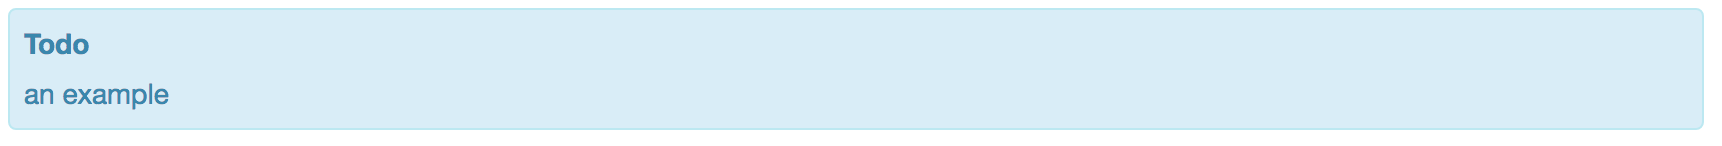
\includegraphics[width=\columnwidth]{../../images/todo.png}

\FILENAME

\section{Markdown}\label{markdown}

The content form this section originates from see:
\url{https://en.wikipedia.org/wiki/Markdown}.

Markdown is a simple markup language, however there is no precise
standard defined for it and implementations may have features not
supported by other implementations. Nevertheless, it provieds as imple
and easy way to quicly develop clean looking documents.

There are severla tools that make markdown attractive allowing to
write the text in one window while at the same time seeing the
rendered out put in another.

This includes

\begin{description}

\item[Macdown] An editor for mardown targeted on OSX

\end{description}

To convert the markdown to other formats with \verb|pandoc|

\begin{verbatim}
# Heading

## Sub-heading

### Another deeper heading
 
Paragraphs are separated
by a blank line.

Two spaces at the end of a line leave a  
line break.

Text attributes _italic_, *italic*, __bold__, **bold**, `monospace`.

Horizontal rule:

---

Bullet list:

  * apples
  * oranges
  * pears

Numbered list:

  1. apples
  2. oranges
  3. pears

A [link](http://example.com).

\end{verbatim}

\subsection{Tools}

\begin{description}
\item [Dilinger] \URL{https://dillinger.io/}. A HTML5 based cloud
  enabled editor. It allows to download the created Markdown.
\item[Macdown] \URL{https://macdown.uranusjr.com/} ``MacDown is an
  open source Markdown editor for macOS''
\end{description}
\FILENAME

\section{Communicating Research in Other Ways}\label{communicating-research}

Naturally, writing papers is not the only way to communicate your
research with others. We find that today we see additional pathways
for cumminication includine blogs, twitter, facebook, e-mail, Web
pages, and electronic notebooks. Let us refisit some of them and
identify when they are helpful.

\subsection{Blogs}\label{blogs}

\begin{description}
\item[blog:]
noun, a regularly updated website or web page, typically one run by an
individual or small group, that is written in an informal or
conversational style.
\end{description}

Advantages:

\begin{itemize}
\tightlist
\item
  encourages spontaneous posts
\item
  encourages small short contributions
\item
  chronologically ordered
\item
  standard software exists to set up blogs
\item
  online services exists to set up blogs
\end{itemize}

Disadvantages:

\begin{itemize}
\tightlist
\item
  structuring data is difficult (some blog software support it)
\item
  not suitable for formal development of a paper
\item
  often lack of sophisticated track change features
\item
  no collaborative editing features
\end{itemize}

\subsection{Sphinx}\label{sphinx}

Sphinx (\url{http://www.sphinx-doc.org/}) is a tool that to create
integrated documentation from a markup language whlie.

Advantages:

\begin{itemize}
\tightlist
\item
  output formats: html, LaTeX, PDF, ePub
\item
  integrates well with directory structure
\item
  powerful markup language (reStructuredText)
\item
  can be hosted on github via github pages
\item
  can integare other renderers such as Markdown
\item
  automatic table of content, tebale of index
\item
  code documentation integration
\item
  search
\item
  written in python and using bash, so extensions and custom automation
  are possible
\end{itemize}

Disadvantage:

\begin{itemize}
\tightlist
\item
  requires compile step
\item
  When using markdown github can render individual page
\end{itemize}

Others:

\begin{itemize}
\tightlist
\item
  Read the Docs (\url{https://readthedocs.org/})
\item
  Doxygen (\url{http://www.stack.nl/~dimitri/doxygen/})
\item
  MkDocs (\url{http://www.mkdocs.org/})
\end{itemize}

\subsection{Notebooks}\label{notebooks}

\subsubsection{Jupyter}\label{jupyter}

The Jupyter Notebook (\url{http://jupyter.org/}) is an open-source web
application allowing users to create and share documents that contain
live code, equations, visualizations and explanatory text. Use cases
include data cleaning and transformation, numerical simulation,
statistical modeling, machine learning.

Advantages:

\begin{itemize}
\tightlist
\item
  Integrates with python
\item
  Recently other programming languages have been integrated
\item
  Allows experimenting with settings
\item
  Allows a form of literate programming while mixing documentation with
  code
\item
  automatically renders on github
\item
  comes with web service that allows hosting
\end{itemize}

Disadvantage:

\begin{itemize}
\tightlist
\item
  mostly encourages short documents
\item
  mark up language is limited
\item
  editing in ASCII is complex and Web editing is prefered
\end{itemize}

\subsubsection{Apache Zeppilin}\label{apache-zeppilin}

A Web-based notebook that enables data-driven, interactive data
analytics and collaborative documents with SQL, Scala and hadoop. It
integrates a web-based notebook with data ingestion, data exploration,
visualization, sharing and collaboration features to Hadoop and Spark.

Advantages:

\begin{itemize}
\tightlist
\item
  integration to various framework
\item
  Web framework
\item
  integration with spark, hadoop
\end{itemize}

Disadvantages:

\begin{itemize}
\tightlist
\item
  larger framework
\item
  must leverages existing deployments of spak, hadoop
\end{itemize}


\begin{comment}
\subsection{References}\label{references}

Collaboratories:

\begin{itemize}
\tightlist
\item
  Myers JD, TC Allison, SJ Bittner, BT Didier, M Frenklach, WH Green, YL
  Ho, J Hewson, WS Koegler, CS Lansing, D Leahy, M Lee, R McCoy, M
  Minkoff, S Nijsure, G von Laszewski, D Montoya, L Oluwole, CM
  Pancerella, R Pinzon, W Pitz, LA Rahn, B Ruscic, KL Schuchardt, EG
  Stephan, A Wagner, TL Windus, and C Yang. 2005. ``A Collaborative
  Informatics Infrastructure for Multi-scale Science.'' Cluster
  Computing 8(4):243-253.
\item
  Metadata in the Collaboratory for Multi-Scale Chemical Science Carmen
  Pancerella, John Hewson, Wendy Koegler, David Leahy, Michael Lee,
  Larry Rahn, Christine Yang, James D. Myers, Brett Didier, Renata
  McCoy, Karen Schuchardt, Eric Stephan, Theresa Windus, Kaizar Amin,
  Sandra Bittner, Carina Lansing, Michael Minkoff, Sandeep Nijsure,
  Gregor von Laszewski, Reinhardt Pinzon, Branko Ruscic, Al Wagner,
  Baoshan Wang, William Pitz, Yen-Ling Ho, David Montoya, Lili Xu,
  Thomas C. Allison, William H. Green, Jr., Michael Frenklach
  \url{http://dcpapers.dublincore.org/pubs/article/view/740/736}
\end{itemize}
\end{comment}



%%----------------------------------------------------------------------------------------
%	PART
%----------------------------------------------------------------------------------------

\part{Documenting Scientific Research}



%----------------------------------------------------------------------------------------
%	CHAPTER 1
%----------------------------------------------------------------------------------------

\chapterimage{writing.png} % Chapter heading image

\chapter{Documenting Scientific Research}
\label{c:doc}

\FILENAME

\FILENAME

\section{Plagiarism}\label{S:plagiarism}

We start with the review of a most important topic.

\subsection{Plagiarism Definition}

In academic life it is important to understand and avoid plagiarism.
The dictionary defines plagiarism as follows \url{dictionary.com}:

% \textipa{['pl\=aj@""riz@m]}

\begin{description}
\item[pla·gia·rism] ``the practice of taking someone else's work or ideas and passing them
off as one's own.''
\end{description}



\subsection{Plagiarism Policies}
Organizations and universities will have policies in place do address
plagiarism. An example is provided for Indiana University
\cite{www-iu-plagiarism}. We quote:

\begin{quotation}
``Honesty requires that any ideas or materials taken from
another source for either written or oral use must be fully
acknowledged. Offering the work of someone else as one’s own is
plagiarism. The language or ideas thus taken from another may range
from isolated formulas, sentences, or paragraphs to entire articles
copied from books, periodicals, speeches, or the writings of other
students. The offering of materials assembled or collected by others
in the form of projects or collections without acknowledgment also is
considered plagiarism. Any student who fails to give credit for ideas
or materials taken from another source is guilty of plagiarism. 

(Faculty Council, May 2, 1961; University Faculty Council, March 11,
1975; Board of Trustees, July 11, 1975)''
\end{quotation}

Faculty members at Universitys are also bound by policies that mandate
reporting. At Indiana University the following policy applies (for a
complete policy see the Web page):

\begin{quotation}
``Should
the faculty member detect signs of plagiarism or cheating, it is his
or her most serious obligation to investigate these thoroughly, to
take appropriate action with respect to the grades of students, and
\textit{in any event} to report the matter to the Dean for Student Services [or
equivalent administrator]. The necessity to report every case of
cheating, whether or not further action is desirable, arises
particularly because of the possibility that this is not the student’s
first offense, or that other offenses may follow it. Equity also
demands that a uniform reporting practice be enforced; otherwise, some
students will be penalized while others guilty of the same actions
will go free.

(Faculty Council, May 2, 1961)''
\end{quotation}

Naturally if a student has any questions about understanding
plagiarism the University can provide assistance. If a student is in
doubt and asks for help this is not considered at that time
plagiarism. 

As you can see from the previous policies, the faculty do not have any
choice but reporting real cases of plagiarism to the university
administration.  Thus you must not hold them personally responsible as
this is part of the tasks they are required to do if they like it or
not. Instead, it is {\bf the responsibility of the authors of the
  document} to assure no plagiarism occurs. If you are a student of a
class that writes a paper or project report this naturally also all
applies to you. In addition, if you work in a team you need to assure
the entire team addresses plagiarism appropriately.

In practice this means that the teachers of a course expect yo know
plagiarism and you need to be informed about it. This is typically
done in other courses. However, as it is often overlooked by the
student we are pointing it out here so we can make sure you contribute
to courses that require you to write papers and reports. This also
means you can not claim you did not know what plagiarism is. You are
required to know what it is, know how to detect it and know how to
avoid it. The resources provided next will give you the necessary
tools and background.

\subsection{Plagiarism Resources}

The \href{http://education.indiana.edu/}{School of Education at Indiana
University} has a significant set of resources to get educated about
plagiarism. These resources are intended to ``preparing educators,
advancing knowledge, and improving education'' \cite{}
\url{https://www.indiana.edu/~istd/patterns.html}

The content here is copied from the Web Page

  \URL{https://www.indiana.edu/~istd/patterns.html}

As such we have not included quotes but refer to their Web page for the
original source which may also include updates. Naturally we do not want
to be accused of plagiarize in a chapter about plagiarism.  Thus assume
the content for the rest ov this chapter are copied from that Web page.

\subsection{Pattern}\label{pattern}

\begin{itemize}
\item
  \href{https://www.indiana.edu/~istd/definition.html}{IU Definition} of
  Plagiarism from Student Code of Conduct
\item
  \href{https://www.indiana.edu/~istd/overview.html}{Overview} How to
  give proper credit, steps.
\item
  \href{https://www.indiana.edu/~istd/cases.html}{Cases} of Plagiarism
  in the US, in the news, and elsewhere
\item
  \href{https://www.indiana.edu/~istd/examples.html}{Examples} Word for
  word, paraphrasing
\item
  \href{https://www.indiana.edu/~istd/practice.html}{Practice} with
  feedback on word-for-word and paraphrasing plagiarism
\item
  \href{https://www.indiana.edu/~istd/test.html}{Test} 10 questions on
  recognizing plagiarism
\item
  \href{https://www.indiana.edu/~istd/sitemap.html}{Tutorial Site Map}
  Expanded table of contents
\item
  \href{https://www.indiana.edu/~istd/resources.html}{Resources}
  Websites, books, dictionary links, references for learning more about
  plagiarism
\end{itemize}

\subsection{Tutorials}\label{S:ptutorial}

A number of tutorials are offerd by Indiana University \href{http://education.indiana.edu/graduate/programs/instructional-systems/index.html}{Instructional
  Systems Technology Department}
 Web pages ealing with plagiarism. Thes include:

\begin{itemize}
\item
  \href{https://www.indiana.edu/~academy/firstPrinciples/choice.html}{Plagiarsim
    Tutorial}
\item
  \href{https://www.indiana.edu/~tedfrick/plagiarism/}{Understanding
  Plagiarism}
\end{itemize}

\subsection{How to Recognize Plagiarism}

We are listing fifteen patterns of plagiarism that are defined on the Web
pages itedntified in Section~\ref{S:ptutorial}:

\begin{tabular}{p{4cm}p{3cm}p{8cm}}
Name & Plagiarism Type & Reason \\
\hline
  \href{patternCluelessQuote.html}{Clueless Quote} &  word-for-word & no
  quotes, no citation, no reference 
\\
  \href{patternCraftyCoverUp.html}{Crafty Cover-up} &  proper paraphrase
  but word-for-word  &  also present
\\
  \href{patternCunningCoverUp.html}{Cunning Cover-up} &  paraphrasing & no
  citation, no reference
\\
  \href{patternDeceptiveDupe.html}{Deceptive Dupe} &  word-for-word  &  no
  quotes, no citation, but has reference
\\
  \href{patternDisconnectedDupe.html}{Delinked Dupe} &  word-for-word  &  no
  reference, even though quotes and citation
\\
  \href{patternDeviousDupe.html}{Devious Dupe} &  correct quote but word-for-word  & 
  also present
\\
  \href{patternDippyDupe.html}{Dippy Dupe} &  word-for-word  &  quotes
  missing, even though full citation and reference
\\
  \href{patternDisguisedDupe.html}{Disguised Dupe} &  looks like proper
  para, but actually word-for-word  &  no quotes, no locator
\\
  \href{patternDoubleTrouble.html}{Double Trouble} & word-for-word  and
  paraphrasing  & although has reference
\\
  \href{patternLostLoser.html}{Linkless Loser} &  word-for-word  &  citation
  and reference lacking, although has quotes and locator
\\
  \href{patternLostLocator.html}{Lost Locator} &  word-for-word  &  missing
  locator, although has quotes, citation, and reference
\\
  \href{patternPointlessParaphrase.html}{Placeless Paraphrase} &  paraphrasing  & 
  no reference, although citation present
\\
  \href{patternSeveredCite.html}{Severed Cite} &  paraphrasing  &  reference
  but no citation
\\
  \href{patternShirkingCite.html}{Shirking Cite} &  word-for-word  &  lacks
  locator and reference, although quotes and citation present
\\
  \href{patternTripleD.html}{Triple D--Disguised Disconnected Dupe} & 
  word-for-word  & looks like proper para, but no quotes, no reference, no locator
\end{tabular}

In addition they do specify  three patterns of
non-plagiarism:

\begin{tabular}{p{2cm}p{4cm}p{8cm}}
Name & Type & Description \\
\hline
\\
  \href{patternCorrectQuote.html}{Correct Quote} &  non-plagiarizm & takes another's words
  verbatim and acknowledges with quotation marks, full in-text citation
  with locator, and reference
\\
  \href{patternProperParaphrase.html}{Proper Paraphrase} &  non-plagiarizm & summarizes
  another's words and acknowledges with in-text citation and reference
\\
  \href{patternMindlessParaphrase.html}{Parroted Paraphrase} &  non-plagiarizm & appears to
  be paraphrasing, and technically may not be plagiarism, but \ldots{}
  ???
\end{tabular}


\FILENAME

\section{Acknowledgements}
\label{S:acknowledgements}

In many cases you want to include an acknowledgement section. In some cases you may be tempted to eliminate this section as you think you are out of space and the acknowledgement section may give you some additional space. This however is the wrong strategy and you should not do this. Instead you should shorten your paper elsewhere and leave enough space for acknowledgements.

In some cases where you get financial support from a university for a project such as from NIH or NSF specific information {\bf must} be included. The best way is to verify with your coauthors. Additional acknowledgements may have to be added and you need te evaluate if for example significant help on the paper warrants co-authorship.

An issue that we have seen often is for example when a professor has helped significantly on the paper but is not properly acknowledged. This can even lead to the professor asking you to remove him from the acknowledgement. A bad acknowledh]gement example is the following:

\begin{quote}
We like to thank Professor Zweistein for his help in compiling  the \LaTeX paper.
\end{quote}

We do not think that the professor will be happy with this acknowledgement as it sounds like the only thing that was provided was the help on LaTeX that you should have done anyways without the help of the professor. Ask yourself, if he introduced you to the field, has helped you with preparing the text, has given you insights, has corrected things in your paper, made suggestions. So instead of the above maybe a more general term such as {\em helped with the paper} would be more appropriate. If not leaving it off is more appropriate. In some cases you may wan to invite your professor to become a co-author. 

\FILENAME

\section{Writing a Scientific Article or Conference Paper}
\index{Writing}

An important part of any scientific research is to document it. This is
often done through scientific conferences or journal articles. Hence it
is important to learn how to prepare and submit such papers. Most
conferences accept typically the papers in PDF format but require the
papers to be prepared on MSWord or in LaTeX. While working with many
students in the past we noticed however that those students using Word
often spend unnecessarily countless hours on trying to make there papers
beautiful while actually violating the template provided by the
conference. Furthermore, we noticed that the same students had issues
with bibliography management. Instead of Word helping the student it
provided the illusion to be easier than LaTeX but when adding up the
time spend on the paper we found that LaTeX actually saved time. This
has been especially true with the advent of collaborative editing
services such as sharelatex \cite{www-sharelatex} and overleaf
\cite{www-overleaf}. 

In this section we provide you with a professional template that is used
for either system based on the ACM standard that you can use to write
papers. Naturally this will be extremely useful if the quality of your
research is strong enough to be submitted to a conference. We structure
this section as follows. Although we do not recommend that you use
MSWord for your editing of a scientific paper, we have included a short
section about it and outline some of its pitfalls that initially you may
not think is problematic, but has proven to be an issue with students.
Next we will focus on introducing you to LaTeX and showcasing you the
advantages and disadvantages. We will dedicate an entire section on
bibliography management and teach you jhow to use jabref which clearly
has advantages for us.

Having a uniform report format not only helps the students but allow
allows the comparison of paper length and effort as part of teaching a
course. We have added an entire section to this chapter that discusses
how we can manage a \emph{Class Proceedings} form papers that are
contributed by teams in the class.

\subsection{Professional Paper Format}\label{professional-paper-format}

The report format we suggest here is based on the standard ACM
proccedings format. It is of very high quality and can be adapted for
your own activities. Moreover, it is possible to use most of teh text to
adapt to other formats in case the conference you intend to submit your
paper to has a different format. The ACM format is always a good start.

Important is that you do not need to change the template but you can
change some parameters in case you are not submitting the paper to a
conference but use it for class papers. Certainly you should not change
the spacing or the layout and instead focus on writing content. As for
bibliography management we recommend you use jabref which we will
introduce in Section \ref{??}.

We recommend that you carefully study the requirements for the report
format. We would nat want that your paper gets rejected by a journal,
conference or the class just because you try to modify the format or do
not follow the established publication guidlines.

The template we are providing is available from:

\URL{https://github.com/cloudmesh/classes/tree/master/docs/source/format/report}

Convenient compressed files are available at

\URL{https://github.com/cloudmesh/classes/tree/master/docs/source/format/report.tar.gz}
\URL{https://github.com/cloudmesh/classes/tree/master/docs/source/format/report.zip}

You will find in it a modified ACM proceedings templates for Word and
for LaTeX that has an identification box removed on the lower left hand
side of the first page. This is done for classes so that you have more
space to write. In case you must submit to a conference you can use the
original ACM template. This template can be found at

\subsection{Submission Requirements}\label{submission-requirements}

Although the initial requirement for some conferences or journals is the
document PDF, in many cases you must be prepared to provide the source
when submitting to the conference. This includes the submission of the
original images in an images foder. You may ba asked to package the
document into a folder with all of its sources and submit to the
conference for professional publication.

\subsection{Microsoft Word vs. \LaTeX}\label{microsoft-word}

Microsoft word will provide you with the initial impression that you
will safe lots of time writing in it while you see the layout of the
document. This will be initially true, but once you progress to the
more challenging parts and later pages such as image menagement and
bibliography management you will see some issues. Thes include that
figure placement in Word need sto be done just right in order for images
to be where they need. We have seen students spending hours with the
placement of figures in a paper but when they did additional changes the
images jumped around and were not at the place where teh students
expected them to be. So if you work with images, make sure you
understand how to place them. Also always use relative caption counters
so that if an image gets placed elsewhere the counter stays consistent.
So nefer use just the number, but a reference to the figure when referring
to it. Recently a new bibliography management system was added to Word.
However, however it is not well documented and the references are placed
in the system bibliography rather than a local managed bibliography.
This mah have severe consequences when working with many authors on a
paper. The same is true when using Endnote. We have heard in many
occasions that the combination of endnote and Word destroyed documents.
You certainly do not want that to happen the day before your deadline.
Also in classes we observed that those using LaTeX deliver better
structured and written papers as the focus is on text and not beautiful
layout.

For all these reasons we do not recommend that you use Word.

In LaTeX where we have an easier time with this as we can just ignore
all of these issues due to relative good image placement and excellent
support for academic reference management. Hence, it is in your best
interest to use LaTeX. The information we provide here will make it easy
for you to get started and write a paper in no time as it is just like
filling out a form.

\subsection{Working in a Team}\label{working-in-a-team}

Today research is done in potentially large research teams. This also
include the writing of a document. There are multiple ways this is done
these days and depends on the system you chose.

In MSWord you can use skydrive, while for LaTeX you can use sharelatex
and overleaf. However, in many cases the use of github is possible as
the same groups that develop the code are also familiar with github.
Thus we provide you here also with the introduction on how to write a
document in github while group members can contribute.

Here are the options:

\begin{description}

\item [LaTeX and git:] This option will likely safe you time as you can use
  jabref also for managing collaborative bibliographies and
\item [sharelatex:] an online tool to write latex documents
\item [overleaf:] an online tool to write latex documents
\item [MS onedrive:] It allows you to edit a word document in collaboration.
  We recommend that you use a local installed version of Word and do the
  editing with that, rather than using the online version. The online
  editor has some bugs. See also (untested):
  \url{http://www.paulkiddie.com/2009/07/jabref-exports-to-word-2007-xml/},
  \url{http://usefulcodes.blogspot.com/2015/01/using-jabref-to-import-bib-to-microsoft.html}
\item [Google Drive:] google drive could be used to collaborate on text that
  is than pasted into document. However it is just a starting point as
  it does not support typically the format required by the publisher.
  Hence at one point you need to swithc to one of the other systems.
\end{description}

\subsection{Timemanagement}\label{timemanagement}

Obviously writing a paper takes time and you need to car-fully make sure
you devote enough time to it. The important part is that the paper
should not be an after thought but should be the initial activity to
conduct and execute your research. Remember that

\begin{enumerate}

\item  It takes time to read the information
\item  It takes time understand the information
\item  It takes time to do the research

\end{enumerate}

For deadlines the following will get you in trouble:

\begin{enumerate}

\item
  \emph{There are still 10 weeks left till the deadline, so let me start
  in 4 week \ldots{}}. Procrastination is your worst enemy.
\item
  If you work in a team that has time management issues address them
  immediately
\item
  Do not underestimate the time it takes to prepare the final submission
  into the submission system. Prepare automated scripts that can deliver
  the package for submission in minutes rather than hours by hand.
\end{enumerate}

\subsection{Paper and Report Checklist}\label{paper-checklist}
\index{Writing!Checklist}

In this section we summarize a number of checks that you may perform to
make sure your paper is properly formatted and in excellent shape.
Naturally this list is just a partial list and if you find things we
should add here, let us know.

\begin{itemize}[label=$\Box$]

\item Have you written the report in the specified format?

\item Have you included an acknowledgement section?

\item Have you included the paper in the submission system (In our
  case git). This includes all images, bibliography files and other
  material that is needed to build the paper from scratch?

\item Have you added the bibliography file that you managed (In our
  case jabref to make it simple for you)?

\item Have you specified proper identification in the submission
  system for your submission.  This is typically a form or ASCII text
  that needs to be filled out and follows a very particular format.
  In our case it is a README.md file that ncludes a homework ID, names
  of the authors, and e-mails)?

\item In case you used word have you also provided the jabref?

\item In case of a class and if you do a multi-author paper, have you
  added a work-breakdown section in the appendix describing who did
  what in the paper?

\item IN case you have an appenix it is included fater the bibliography

\item Have you spellchecked the paper?

\item Have you grammar chacked the paper?

\item Are you using \textbf{a} and \textbf{the} properly?

\item Have you made sure you do not plagiarize?

\item Is the title properly capitalized?

\item Have you not used phrases such as shown in the Figure below, but
  instead used as shown in Figure 3 when referring to the 3rd figure?
  Numbers in LaTeX are done with \verb|\label{}| after captions and
  \verb|\ref{}| in the text (See examples in the LaTeX section). In
  word you must use relative numbering.

\item Have you capitalized ``Figure 3'', ``Table 1''?

\item Have you removed any figure that is not referred explicitly in
  the text. E. ech figure needs a text such as  {\em As shown in
    Figure ..} or similar.

\item Are the figure captions bellow the figures and not on top. (Do
  not include the titles of the figures in the figure itself but
  instead use the caption or that information?

\item When using tables have you put the table caption above the table?

\item When using image have you put the table caption bellow the image?

\item Make the figures large enough so we can read the details. If
  needed make the figure over two columns? 

\item Do not worry about the figure placement if they are at a
  different location than you think. Figures are allowed to float. In
  many submissions you may have to place all figures at the end of the
  paper so you can focus on content rather than placing figures. In
  addition it will help you to refer to the figures by index.

\item Are all figures and tables at the end?

\item In case you copied a figure from another paper you need to ask
  for copyright permission. In case of a class paper you \textbf{must}
  include a reference to the original at the end of the figure caption.

\item Do not use the word ``I'' instead use ``we'' even if you are the
  sole author.

\item Do not use the phrase ``In this paper/report we show'' instead
  use ``We show''. It is not important if this is a paper or a report
  and does not need to be mentioned.

\item Do not artificially inflate your paper if you are bellow the
  page limit and have nothing to say anymore.

\item If your paper limit is 12 pages but you want to hand in 120
  pages, please check first ;-) If your page limoit is 2 pages but you
  hand in 4 thats is no issue.

\item Do not use the characters \& \# \% \_  in the paper if you use
  LaTeX. If you use them you probably need a bakslash in front of them.

\item Latex uses double single open quotes and double single closed
  quotes for quotes. Have you made sure you replaced them?

  When using quotes in LaTeX, do not use the double quote but instead
  use two single quotes such as \verb|``This is a quote''|. THis will
  place the proper quotes in the text. To only use the quotes when you
  literraly quote from other papers. Never use a quote to emphasize a
  thext. For that you use \verb|{\em this is emphasize}| resulting in
  {\em This is emphasized}.

\item If you want to say and do not use \& but use the word {\em
    and}. If you need tou use it be reminded to write it as \verb|\&|


\item Pasting and copying from the Web often results in non ascii
  characters to be used in your text, please remove them and replace
  accordingly. This includes some form of -- that you may see showing
  up as fi in pdf

\item Is your Abstract not a proposal? Abstracts are no proposals, e.g
  This paper intends to show .... If the paper intends to show you are
  still in the draft phase of the paper. However, if you say We sow
  ... That would be good. Let us just assume you intended to show
  something but did not achieve then you can say We intended to show
  this but we showed it was not possible. As you can see not only the
  intention is communicated, but the result. If you just focuss on the
  intent that's just a proposal and is not a proper abstract.

\item Are you not using the word paper in your writeup?  Abstracts and
  the entire paper should not have the word paper in it.

\item If your paper is an introduction or overview paper, please do
  not assume the reader to be an expert. Provide enough material for
  the paper to be useful for an introduction into the topic. 

\item Are you refernces correct? References to a paper are no
  afterthought, they should be properly cited. Use jabref and make
  sure the citation type of the refernce is correct and fill out as
  many fields as you can. Some jouranls and conferences have for
  example special requirements that go beyond the requirements of for
  example jabref. One example is that maky conferences require you
  that wne you cite papers form another conference to augment the
  conferences not only with the location where the conference took
  place, but also with the dates the conference took
  place. Unfortunately, this is information that is often only
  avalable through additional google quesies and many refernce entries
  you find in the internet do not have this information readily
  available.

\end{itemize}

In case of a class

\begin{itemize}[label=$\Box$] 

\item Check in your current work of the paper on a weekly basis to
  show consistent progress.

\item Please use the dedicated report format for class. It may not be
  the ACM or IEEE format, but may have some additions that make
  management of bibliographies easier. Do follow our instructions for
  bibliographies.

\end{itemize}

In case you are allowed to use word in class, such as the one we teach
at IU, the following applies in addition:

\begin{itemize}[label=$\Box$] 

\item Are you managing your references in jabref and endnote (we need
  both)
\item Are you using the right template we have a special 2 column
  template for the class that is a modified version from the 2 column
  ACM template
\item Are you using build in numbered section management? MSWord has
  Sections that must be used
\item Are you using real bulleted lists in Word and not just a ``*''
  or a ``-''?
\item Have you carelessly pasted and copied into the document without
  using proper formats. E.g. in MSWord this is a problem. You need to
  fix the format and use the build in format. Not that if you paste
  wrong you effect the format styles.
\item Have you created not only a docx document but also the PDF.

\item Make sure you use .docx and not .doc

\end{itemize}

If you observe something missing let us know.

\subsection{Example Paper}\label{example-paper}

An example report in PDF format is available:

\begin{itemize}

\item
  \href{https://github.com/cloudmesh/classes/blob/master/docs/source/format/report/latex/report.pdf}{report.pdf}
\end{itemize}

\subsection{Creating the PDF from LaTeX on your
Computer}\label{creating-the-pdf-from-latex-on-your-computer}

Latex can be easily installed on any computer as long as you have
enough space. Furthermore if your machine can execute the make command
we have provided in the standard report format a simple
\href{https://github.com/cloudmesh/classes/blob/master/docs/source/format/report/latex/Makefile}{Makefile}
that allows you to do editing with immediate preview as documented in
the LaTeX lesson.

\subsection{Class Specific README.md}\label{class-specific-readme.md}

For the class we will manage all papers via github.com. You will be
added to our github at

\URL{https://github.com/bigdata-i523}

and assigned an hid (homework index directory) directory with a unique
hid number for you. In addition, once you decide for a project, you will
aslso get a project id (pid) and a directory in which you place the
projects. Projects must not be placed in hid directories as they are
treated differently and a class proceedings is automatically created
based on your submission.

As part of the hid directory, you will need to create a README.md file
in it, that \textbf{must} follow a specific format. The good news is
that we have developed an easy template that with common sense you can
modify easily. The template is located at

\URL{https://raw.githubusercontent.com/bigdata-i523/sample-hid000/master/README.md}

As the format may have been updated over time it does not hurt to
revisit it and compare with your README.md and make corrections. It is
important that you follow the format and not eliminate the lines with
the three quotes. The text in the quotes is actually yaml. yaml is a
data format the any data scientist must know. If you do not, you can
look it up. However, if you follow our rules you should be good. If you
find a rule missing for our purpose, let us know. We like to keep it
simple and want you to fill out the \emph{template} with your
information.

Simple rules:

\begin{itemize}

\item
  replace the hid nimber with your hid number.
\item naturally if you see sample- in the directory name you need to

  delete that as your directory name does not have sample- in it.
\item do not ignore where the author is to be placed, it is in a list

  starting with a -
\item there is always a space after a -

\item do not introduce empty lines

\item do not use TAB and make sure your editor does not bay accident

  automatically creates tabs. This is probably the most frequent error
  we see.
\item do not use any : \& \_ in the attribute text including titles

\item an object defined in the README.md must have on a single type

  field.  for example in the project section. Make sure you select
  only one type and delete the other
\item in case you have long paragraphs you can use the \textgreater{}

  after the abstract
\item Once you understood how the README.md works, please delete the

  comment section.
\item Add a chapter topic that your paper belongs to

\end{itemize}

\subsection{Exercise}\label{exercise}

\begin{description}
\item[Report.1:]
Install latex and jabref on your system
\item[Report.2:]
Check out the report example directory. Create a PDF and view it. Modify
and recompile.
\item[Report.4:]
Learn about the different bibliographic entry formats in bibtex
\item[Report.5:]
What is an article in a magazine? Is it really an Article or a Misc?
\item[Report.6:]
What is an InProceedings and how does it differ from Conference?
\item[Report.7:]
What is a Misc?
\item[Report.8:]
Why are spaces, underscores in directory names problematic and why
should you avoid using them for your projects
\item[Report.9:]
Write an objective report about the advantages and disadvantages of
programs to write reports.
\item[Report.10:]
Why is it advantageous that directories are lowercase have no underscore
or space in the name?
\end{description}

% \FILENAME

\section{Report Format}\label{report-format}

Although we provide \textbf{trivial} but detailed report format
requirements, we observed over the years that some students still asked
us can I make my report shorter, or can i use a different format? The
answer to these questions is \textbf{no}. Furthermore, we observed that
the same students than went ahead and played with the formating and
introduced empty lines, increased tables or figures, or worse modified
the fontsize to circumvent the page limit requirement.

Thus we have adopted a much simpler approach that is easy to summarize

\begin{enumerate}
\def\labelenumi{\arabic{enumi}.}

\item
  We provide you with a \textbf{high quality} report template format
  that you must not change and is used by millions of researchers.
\item
  All references must be managed with jabref as reference management
  tool and must be provided in addition to the document.
\item
  If your document does not follow the format or we find that you have
  modified the style of the template we provide will return the document
  without review.
\item
  It is in the students responsibility to use the template format from
  the beginning on. In fact, our assignments will use the template for
  all assignments and not just your term paper or term report.
\end{enumerate}

The template for the report is available from:

\begin{itemize}

\item
  \url{https://github.com/cloudmesh/classes/tree/master/docs/source/format/report}
\end{itemize}

Convenient compressed files are available at

\begin{itemize}

\item
  \url{https://github.com/cloudmesh/classes/tree/master/docs/source/format/report.tar.gz}
\item
  \url{https://github.com/cloudmesh/classes/tree/master/docs/source/format/report.zip}
\end{itemize}

You have two choices. A good one and a bad one.

The good choice is to use the LaTeX template and write your document in
LaTeX. The bad one is to use the Word template and write the document in
Word. Both templates are included in our git repository.

Hence, it is in your best interest to use LaTeX. The good news is that
we have made it simple for you to use it. Furthermore, you are allowed
to use online services. An example report in PDF format is available:

\begin{itemize}

\item
  \href{https://github.com/cloudmesh/classes/blob/master/docs/source/format/report/latex/report.pdf}{report.pdf}
\end{itemize}

We provide a very simple
\href{https://github.com/cloudmesh/classes/blob/master/docs/source/format/report/latex/Makefile}{Makefile}
that allows you to do editing with immediate preview as documented in
the LaTeX lesson. Due to LaTeX being a \textbf{trivial} ASCII based
format and having a superior bibliography management you will save
yourself many hours of work that you will face while fighting with Word.
We got feedback from those that tried it and they thanked us later.
Furthermore, in case you are in a team, you can use either git while
collaboratively developing the LaTeX document, use sharelatex, or
overleaf.

However, we allow you to use word under the following conditions:

\begin{enumerate}
\def\labelenumi{\arabic{enumi}.}

\item
  You accept the risk that Word may crash and you may find yourself in
  last minute in the situation that you lost your work and your document
  is broken. We will not be sympathetic to this situation as we
  recommended that you use LaTeX.
\item
  You must use not only Endnote, but also jabref when managing your
  references, so you have to do the management of references twice. This
  is so that your document could be converted to LaTeX in case we think
  it suitable for publication in a conference or workshop.
\item
  You do not modify the theme.
\item
  All images and tables are placed at the end of the paper.
\item
  Git wil be used to submit all documents with regular updates.
\end{enumerate}

For LaTeX you will encounter a much more smooth experience.

\begin{enumerate}
\def\labelenumi{\arabic{enumi}.}

\item
  Your final document must be committed in git and as LaTeX is ASCII
  based you can do thous throughout the semester and have backups via
  git.
\item
  You will be using jabref to manage your bibliography and as LaTeX has
  build in support for bibliography management there is not much you
  need to pay attention to, all Format of the references is done for you
  in case you entered them correctly
\item
  You do not modify our theme.
\item
  All images and tables are placed at the end of the paper.
\item
  Git wil be used to submit all documents.
\item
  You are allowed to use sharelatex or overleave so you do not have to
  install LaTeX on your computer, but see 5. and the next paragraph.
\end{enumerate}

Whatever format you use, your final submission must be in \textbf{the
class} git. We will not review any documents stored on sharelatex or
overleaf or in any git repository not belonging to the class. Your final
submission will include the bibliography file(s) as a separate
document(s). All images must be placed in an images folder and submitted
in your repository with the originals. When using sharelatex or overleaf
you must replicate the directory layout carefully from our template and
include your final documents in git with a Makefile that can recreate
the document. It is in your responsibility that this works. We will
regenerate the document from source before we grade it. Thus it is not
sufficient to just check in the final PDF. The report must be spell
checked.

\begin{description}
\item[There will be \textbf{NO EXCEPTION} to this. We will not]
review your report if its submission is incomplete.
\end{description}

\subsection{Leverage parallel editing}\label{leverage-parallel-editing}

In most cases you will be able to work in groups on class projects. This
allows you to develop the report collaboratively. Here are some options:

\begin{enumerate}

\item
  LaTeX and git: THis option will likely safe you time as you can use
  jabref also for manageing collaborative bibliographies and
\item
  MS onedrive: It allows you to edit a word document in collaboration.
  We recommend that you use a local installed version of Word and do the
  editiong with that, rather than useing the online verison. The online
  editor has some bugs. See also (untested):
  \url{http://www.paulkiddie.com/2009/07/jabref-exports-to-word-2007-xml/},
  \url{http://usefulcodes.blogspot.com/2015/01/using-jabref-to-import-bib-to-microsoft.html}
\item
  Google Drive: google drive could be used to collaborate on text that
  is than pasted into document. he final document will not accept as
  google document. You must use the 2 column ACM template. We observed
  that students that use google docs lack structure and we no longer
  allow it as final document format. It also does not allow us to
  uniformly compare the documents between each other. It is easy to
  transfer it to LaTeX.
\end{enumerate}

\subsection{Timemanagement Tips}\label{timemanagement-tips}

Obviously taking a class takes time

\begin{enumerate}

\item
  It takes time to read the information
\item
  It takes time understand the information
\item
  It takes time to do the project
\item
  This will get you in trouble: \emph{There are still 10 weeks left till
  the project is due so let me start in 4 weeks \ldots{}}. Postponing
  the project till the last moment
\item
  Do not spend significant time on unimportant documentation and setup.
  Instead spend time to develop cmd5 comamnds and scripts that do these
  things automatically
\end{enumerate}

\subsection{Report Checklist}\label{report-checklist}

This partiald list may serve as a way to check if you follow the rules

\begin{enumerate}

\item
  Have you written the report in the specified format?
\item
  Have you included an acknowledgement section?
\item
  Have you included the report in git?
\item
  Have you specified the HID, names, and e-mails of all team members in
  your report. E.g. the Real Names that are registered in Canvas?
\item
  Have you included the project number in the report?
\item
  Have you included all images in native and PDF format in git in the
  images folder?
\item
  Have you added the bibliography file that you managed with jabref
\item
  In case you used word have you also provided the endnote file
\item
  Have you added an appendix describing who did what in the project or
  report?
\item
  Have you spellchecked the paper?
\item
  Are you useing \textbf{a} and \textbf{the} properly?
\item
  Have you made sure you do not plagiarize?
\item
  Have you not used phrases such as shown in the Figure below, but
  instead used as shown in Figure 3 when referring to the 3rd figure?
\item
  Have you capitalized ``Figure 3'', ``Table 1'', \ldots{} ?
\item
  Any figure that is not referred to explicitly in the text must be
  removed.
\item
  Are the figure captions bellow the figures and not on top. (Do not
  include the titles of the figures in the figure itself but instead use
  the caption or that information?
\item
  When using tables have you put the table caption on top?
\item
  Make the figures large enough so we can read the details. If needed
  make the figure over two columns?
\item
  Do not worry about the figure placement if they are at a different
  location than you think. Figures are allowed to float. If you want you
  can place all figures at the end of the report?
\item
  Are all figures and tables at the end?
\item
  Do not use the word ``I'' instead use we even if you are the sole
  author?
\item
  Do not use the phrase ``In this paper/report we show'' instead use
  ``We show''. It is not important if this is a paper or a report and
  does not need to be mentioned.
\item
  Do not artificially inflate your report if you are bellow the page
  limit and have nothing to say anymore.
\item
  If your paper limit is 12 pages but you want to hand in 120 pages,
  please check first with an instructor ;-)
\item
  Check in your current work of the report on a weekly basis to show
  consistent progress.
\item
  Please use the dedicated report format for class. It may not be the
  ACM or IEEE format, but may have some additions that make management
  of bibliographies easier. Do follow our instructions for
  bibliographies.
\item
  Do not use the characters \& \# \% in the paper if you use LaTeX. If
  you use them you prabably need a in front of them.
\item
  If you want to say and do not use \& but use the word and.
\item
  (I524) Is in your report directory a README.rst file in it as shown in
  the example project that we introduced you to?
\item
  (I523) you do not have to place a readme in your report or paper
  directories. Instead create a README.md in your hid or pid
  directories.
\end{enumerate}

If you observe something missing let us know.

In case you are allowed to use word The following applies in addition

\begin{enumerate}

\item
  Are you manageing your refernces in jabref and endnote (we need both)
\item
  Are you using the right template we have a special 2 column template
  for the class that is a modified version from the 2 column ACM
  template
\item
  Are you using build in numbered section management? MSWord has
  Sections that must be used
\item
  Are you using real bulleted lists in Word and not just a ``*'' or a
  ``-''?
\item
  Have you carelessly pasted and copied into the document without using
  proper formats. E.g. in MSWord this is a problem. You need to fix the
  format and use the build in format. Not that if you paste wrong you
  effect the format styles.
\item
  Have you created not only a docx document but also the PDF.
\item
  Make sure you use .docx and not .doc
\end{enumerate}

If you have other things to add, send them via piazza and we will add
them here.

\subsection{README.md}\label{readme.md}

For I523, Fall 2017, we will manage all papers via github.com. You will
be added to our github at

\begin{itemize}

\item
  \url{https://github.com/bigdata-i523}
\end{itemize}

and assigned an hid (homework index directory) directory with a unique
hid number for you. In addition, once you decide for a project, you will
aslso get a project id (pid) and a directory in which you place the
projects. Projects must not be placed in hid directories as they are
treated differently and a class proceedings is automatically created
based on your submission.

As part of the hid directory, you will need to create a README.md file
in it, that \textbf{must} follow a specific format. The good news is
that we have developed an easy template that with common sense you can
modify easily. The template is located at

\begin{itemize}

\item
  \url{https://raw.githubusercontent.com/bigdata-i523/sample-hid000/master/README.md}
\end{itemize}

As the format may have been updated over time it does not hurt to
revisit it and compare with your README.md and make corrections. It is
important that you follow the format and not eliminate the lines with
the three quotes. The text in the quotes is actually yaml. yaml is a
data format the any data scientist must know. If you do not, you can
look it up. However, if you follow our rules you should be good. If you
find a rule missing for our purpose, let us know. We like to keep it
simple and want you to fill out the \emph{template} with your
information.

Simple rules:

\begin{itemize}

\item
  replace the hid nimber with your hid number.
\item
  naturally if you see sample- in the directory name you need to delete
  that as your directory name does not have sample- in it.
\item
  do not ignore where the author is to be placed, it is in a list
  starting with a -
\item
  there is always a space after a -
\item
  do not introduce empty lines
\item
  do not use TAB and make sure your editor does not bay accident
  automatically creates tabs. This is probably the most frequent error
  we see.
\item
  do not use any : \& \_ in the attribute text including titles
\item
  an object defined in the README.md must have on a single type field.
  for example in the project section. Make sure you select only one type
  and delete the other
\item
  in case you have long paragraphs you can use the \textgreater{} after
  the abstract
\item
  Once you understood how the README.md works, please delete the comment
  section.
\end{itemize}

\subsection{README.rst (for I524, Spring
2017)}\label{readme.rst-for-i524-spring-2017}

In the directory that containes the report, please include the following
README.rst file. Without this file we will not review your document:

\begin{verbatim}
Title: The title of your paper (one line)

Author: The author s of the paper (one line)

HID: The HID of the authors in the order as specified in authors (one line)

PID: The PID of the paper (there will be exactly one)

E-mail: The e-mails of the authors in the order of the author list (one line)

Format: latex or word (specify one)
\end{verbatim}

Please note that all information has an empty line between them and all
information is stored in one line

This information is used to autogenerate the class proceedings.

\subsection{Exercise}\label{exercise}

\begin{description}
\item[Report.1:]
Install latex and jabref on your system
\item[Report.2:]
Check out the report example directory. Create a PDF and view it. Modify
and recompile.
\item[Report.4:]
Learn about the different bibliographic entry formats in bibtex
\item[Report.5:]
What is an article in a magazine? Is it really an Article or a Misc?
\item[Report.6:]
What is an InProceedings and how does it differ from Conference?
\item[Report.7:]
What is a Misc?
\item[Report.8:]
Why are spaces, underscores in directory names problematic and why
should you avoid using them for your projects
\item[Report.9:]
Write an objective report about the advantages and disadvantages of
programs to write reports.
\item[Report.10:]
Why is it advantageous that directories are lowercase have no underscore
or space in the name?
\end{description}



\chapter{Introduction to \LaTeX}
\label{C:latex}

\FILENAME

Mastering a text processing system is an essential part of a
researcher's life. Not knowing how to use a text processing system can
slow down the productivity of research drastically.

\section{Installation}
\label{installation}
\index{Latex!installation}

LaTeX is available on all modern computer systems. A very good
installation for OSX is available at:

\begin{itemize}
\item
  \url{https://tug.org/mactex/}
\end{itemize}


However, if you have older versions on your systems you may have to
first completely uninstall them.

\subsection{Local Install}\label{local-install}

Installing LaTeX is trivial, and is documented on the internet very
well. However, it requires sufficient space and time as it is a large
environment. A system such as TeX Live takes in full install about 5.5
GB. In addition to LaTeX we recommend that you install jabref and use it
for bibliography management.

Thus you will have the most of them on your system.

\begin{itemize}

\item
  pdflatex: the latex program producing pdf
\item
  bibtex: to create bibliographies
\item
  jabref: GUI application to bibtex files (\url{http://www.jabref.org/})
\end{itemize}

Make sure you check that these programs are there, for example with the
Linux commands:

\begin{verbatim}
which pdflatex
which bibtex
which jabref (on OSX you may have an icon for it)
\end{verbatim}

If these commands are missing, please install them. For the newest
documentation on installation of LaTeX we recommend you look up the
installation for your specific OS.

\subsubsection{Install on Ubuntu 16.04}\label{install-on-ubuntu-16.04}
\index{Latex!installation!ubuntu}

The easiest way to install it on ubuntu is to use the terminal and type
in (make sure you have enough space):

\begin{verbatim}
sudo apt-get install texlive-full
\end{verbatim}

One of the best editors for LaTeX is emacs as you can also do
bibliography management with it and not just LaTeX. However, other
editors are available including:

\begin{itemize}

\item
  Kile, TeXworks, JLatexEditor, Gedit LaTeX Plugin, TeXMaker
\end{itemize}

Please look up how to install them if you like to use them. TeXMaker is
popular, However I find the combination of emacs and latexmk superior.
TeXmaker is installed with:

\begin{verbatim}
sudo apt-get install texmaker
\end{verbatim}

Other installations:

\begin{itemize}

\item
  kile is installed by default
\item
  \url{https://www.tug.org/texworks/} (Works on ubuntu, Windows, OSX)
\end{itemize}

\subsubsection{LaTeX for OSX}\label{latex-for-osx}
\index{Latex!installation!OSX}

\begin{itemize}

\item
  \url{https://www.latex-project.org/get/}
\end{itemize}

\subsubsection{LaTeX for Windows}\label{latex-for-windows}
\index{Latex!installation!Windows}

\begin{itemize}

\item
  \url{https://www.latex-project.org/get/}
\end{itemize}


\URL{https://miktex.org/howto/install-miktex}

\begin{exercise}

Evaluate if you can install \LaTeX~ on Windows. We suggest you start
with miktex. Find out how to install gitbash and make as we have some
makefiles.. we also want to figure out how to instal latexmk

\end{exercise}

\subsection{Online Services}\label{online-services}

\subsubsection{Sharelatex}\label{sharelatex}
\index{Latex!Sharelatex}

ShareLaTeX is an online, collaborative LaTeX editor that makes the
creation, preview, and sharing of LaTeX documents easy through a
web-based interface.  Those that like to use latex, but do not have it
installed on their computers may want to look at the following video:

Video: \url{https://youtu.be/PfhSOjuQk8Y}

Video with cc: \url{https://www.youtube.com/watch?v=8IDCGTFXoBs}

ShareLaTeX not only allows you to edit online, but allows you to share
your documents in a group of up to three. Licenses are available if you
need more than three people in a team.

\paragraph{IU Licensed ShareLaTeX}

At IU we has a license for the ShareLaTeX service available to School
of Informatics and Computing and Engineering students, faculty, and
staff only on the Bloomington campus.  

You can create a free ShareLaTeX account but the free accounts have
limitations.  Adding your account to the IU license will give you access
to advanced features, including unlimited sharing.  
It will also allow GitHub integration. THis however only works with
the commercial github.com and not the IU Enterprise GitHub at
github.iu.edu. As we require in our courses github.com you will be
able to use it.

\textit{Please note that this license is only available to School of
Informatics and Computing students, faculty, and staff on the
Bloomington campus.  Students must be enrolled in one of the SoIC
degree programs on the Bloomington campus to be eligible.  Students in
other degree programs (even those taking SoIC classes) are not
eligible.}


If you want to use this service, please do and be aware of the following: 

\begin{enumerate}

\item Go to the ShareLaTeX site and register.  Please note that you
  {\bf must} use either an \verb|@indiana.edu| or \verb|@iu.edu| email
  address when you register. If you use any other email address, we
  will not be able to add you to our site license.  You are also
  required to use your IU passphrase as your ShareLaTeX password.
  Once you have registered, send an email to
  \verb|soichelp@indiana.edu| asking to have your sharelatex account 
  added to the IU license.  

\item
  In your request, you must include the following: The IU email
  address you used when you registered (which must be in either the
  \verb|@indiana.edu| or \verb|@iu.edu| domain) A statement indicating
  that you understand that the ShareLaTeX service cannot be used for
  any sensitive data

\item Note that the ShareLaTeX service is {\bf not} qualified for any
  sensitive data. This includes all data in the Critical, Restricted,
  and University-Internal categories as defined in the Data
  Classifications Page.

\end{enumerate}


\subsubsection{Overleaf}\label{overleaf}
\index{Latex!overleaf}

Overleaf.com is a collaborative latex editor. In its free version it has
a very limited disk space. However it comes with a Rich text mode that
allows you to edit the document in a preview mode. The free templates
provided do not include ACM template, put you are allowed to use the OSA
template.

Features of overleaf are documented at:
\url{https://www.overleaf.com/benefits}

\subsubsection{Paperia}\label{paperia}

We do not know where this service is located. However it offers similar
services as ShareLatex and Overleaf.

\begin{itemize}

\item
  \url{https://papeeria.com/}
\end{itemize}


\section{Basic LaTeX Elements}\label{latex}
\index{Latex!Elements}

Often researchers may be initially overwhelmed with all the features
that \LaTeX~ provides. However, it is much simpler than you initially
believe. In Chapter ?? we introduced you towards using an article
template. As a template is provided you can just look at the elements
in that article and modify or copy them while adapting the
content. Thus, it is more like filling out a form. You do not have to
learn much and you can learn as you go. We are providing in this
chapter some basic \LaTeX~ elements that will help you getting started
quickly while serving you as a reminder what how to do certain things
in \LaTeX~.



\subsection{Characters}\label{characters}
\index{Latex!\%}
\index{Latex!\$}
\index{Latex!\#}
\index{Latex!\_}

LaTeX is a command language and as such uses some special characters as
part of the language. Thus if you want to use these characters either in
your text or bibliography you need to be especially carful about. These
characters include \% \$ \# \_

Other than in hyperref links and urls you need to put a backslash in
front of them. For example to print a \% in the text you need to use:

\begin{verbatim}
\%
\end{verbatim}

Furthermore the character \verb|"| is not at all used as discussed in the next
section.

\subsection{Highlighting Text}\label{highlighting-text}
\index{Latex!Elements!highlight text}

Quotes are not written with the \verb|"| character, but are embedded in two
left single quotes and two right single quotes:



\begin{tcblisting}{colback=blue!5!white,colframe=gray!50!blue,listing side text,
  title=quote,fonttitle=\bfseries}
``This is a quote''
\end{tcblisting}



In many papers we see that the quote is misused while putting quotes
around a word. However quotes are often just used to quote a text from
another paper. Instead of using quotes authors may actually emphasize a
word. LaTeX has a special command for that using:

\begin{tcblisting}{colback=blue!5!white,colframe=gray!50!blue,listing side text,
  title=emphasize,fonttitle=\bfseries}
\textit{this is emphasized}
\end{tcblisting}

To write a text as bold (which should also be avoided as bold is
typically used in section headers), you can use:

\begin{tcblisting}{colback=blue!5!white,colframe=gray!50!blue,listing side text,
  title=bold fett,fonttitle=\bfseries}
{\bf this is bold fett}
\end{tcblisting}

\subsection{Sections}\label{sections}
\index{Latex!Elements!sections}

LaTeX provides a convenient mechanism to structure a paper with sections
and subsections THis is achieved with the following commands:

\begin{verbatim}
\section{This is a Section}
\subsection{This is a Subsection}
\subsubsection{This is a Subsubsection}  
\end{verbatim}

Once you use one of these commands the next paragraph will start bellow
the section command.

In addition you have the command:

\begin{verbatim}
\paragraph{This is a paragraph.}

The line is behind the paragraph heading
\end{verbatim}

The command is special as it does not introduce a new line between the
Heading and the next line even if you include empty lines

\subsection{Empty Lines}\label{empty-lines}

Multiple empty lines will be reduced to a single empty line.

\subsection{Itemize}\label{itemize}
\index{Latex!Elements!itemiz}


Itemized lists can be written as follows:


\begin{tcblisting}{colback=blue!5!white,colframe=gray!50!blue,listing side text,
  title=itemize,fonttitle=\bfseries}
\begin{itemize}
   \item First item
   \item Second item
\end{itemize}
\end{tcblisting} 


\subsection{Enumerate}\label{enumerate}
\index{Latex!Elements!enumerate}

Enumerations can be written as:

\begin{tcblisting}{colback=blue!5!white,colframe=gray!50!blue,listing side text,
  title=enumerate,fonttitle=\bfseries}
\begin{enumerate}
   \item First item
   \item Second item
\end{enumerate}
\end{tcblisting} 

\subsection{Descriptions}\label{descriptions}
\index{Latex!Elements!description}

Description lists can be written as:

\begin{tcblisting}{colback=blue!5!white,colframe=gray!50!blue,listing side text,
  title=enumerate,fonttitle=\bfseries}
\begin{description}
   \item[Cloud:] My definition of a Cloud is over more than one line
     so we show the indentation.
   \item[Big Data:] My definition of Big Data is also a long description.
\end{description}
\end{tcblisting} 




\subsection{Images}\label{images}
\index{Latex!Elements!images}

Figures are extremely easy to handle by including them from source. We
never worry about the placement as LaTeX does typically a very
good job of doing this.:

\begin{verbatim}
In Figure~\ref{F:flow} we show a black and white graph about ... .

\begin{figure}[htb]
  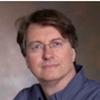
\includegraphics[width=1.0\columnwidth]{images/gregor.png}
  \caption{A demonstration in the scalability of PDF images.}
  \label{F:flow}
\end{figure}
\end{verbatim}

Which results in the following:
\begin{quote}
In Figure~\ref{F:flow} we show a black and white graph about ... .

\begin{figure}[htb]
  \includegraphics[width=1.0\columnwidth]{images/i523-overview.pdf}
  \caption{A demonstration in the scalability of PDF images.}
  \label{F:flow}
\end{figure}
\end{quote}

Note that las17graph must be a label of a valid bibtex entry. This is
needed if you have copied the image from elsewhere to avoid plagiarism.
However, if you came up with the graph yourself than you do not need a
citation.

We recommend that you place in your paper drafts all images at the which
can be done with the endfloat package

This can be enabled if you include the following lines before begin
document command:

\begin{verbatim}
\usepackage{endfloat}
\renewcommand{\efloatseparator}{\mbox{}} 

\begin{document}
\end{verbatim}

\subsection{Tables}\label{tables}
\index{Latex!Elements!tables}

Latex tables are very similar to csv table. Thus you could with
appropriate manipulation create tables from csv tables and use tools
such as spreadsheet editors to manage your table. There are even
packages that allow you to import the contents of csv tables directly
into \LaTeX.

In many cases you simply can start with an online table generator such as

\URL{https://www.tablesgenerator.com/}

For some tables you may want to rescale the width with

\begin{verbatim}
\resizebox{\textwidth}{!}{%
   ... PUT YOUR TABLE HERE ....
}
\end{verbatim}

In other cases you may want to rotate the table which you can easily
google for. In all cases use as figures, tables need to be in the
\verb|table| float environment. In contrast to figures captions are on
the top. All tables must be referred to by \verb|ref|. For more
information in directly including csv tables see 

\URL{http://mirror.utexas.edu/ctan/macros/latex/contrib/csvsimple/csvsimple.pdf}

However the format is very easy and can in most cases directly be
included in latex as shown in Table~\ref{T:elements}.

\begin{verbatim}
\begin{table}[htb]
\caption{Table with elements}\label{T:elements}
\bigskip
\begin{center}
\begin{tabular}{ c c c }
 column1  & column2  & column3 \\
\hline
\hline
 element1 & element2 & element3 \\ 
 element4 & element5 & element6 \\  
 element7 & element8 & element9 \\
\hline
\end{tabular}
\end{center}
\end{table}
\end{verbatim}

\begin{table}[htb]
\caption{Table with elements}\label{T:elements}
\bigskip
\begin{center}
\begin{tabular}{ c c c }
 column1  & column2  & column3 \\
\hline
\hline
 element1 & element2 & element3 \\ 
 element4 & element5 & element6 \\  
 element7 & element8 & element9 \\
\hline
\end{tabular}
\end{center}
\end{table}

\subsection{Labels}\label{labels}
\index{Latex!Elements!labels}

As we saw already for figures and tables it is recommended to use the
label and ref commands to refer to figure or table numbers. This applies
also to sections. Thus I can place a label after a section:

\begin{verbatim}
\section{Introduction}\label{S:introduction}
\end{verbatim}

and write elsewhere in the paper:

\begin{verbatim}
As we showcased in Section~\ref{S:introduction}
\end{verbatim}

Furthermore to conveniently distinguish sections tables and figures, we
use the prefix S T F followed by a colon for the label. This helps
organizing your paper in case you have many labels.

\subsection{Mathematics}\label{math}
\index{Latex!Elements!mathematics}

One of the strength of LaTeX thi the ability to write easily
sophisticated mathematical expressions on paper with high quality. A
good online resource is provided by the following online resource from
which we have copied some examples:

\begin{itemize}

\item
  \url{https://en.wikibooks.org/wiki/LaTeX/Mathematics}
\end{itemize}

To activate them use 

\begin{verbatim}
\usepackage{amsmath}
\end{verbatim}

at the beginning of the document after the document class

Exponents are using the \^{} character:

\begin{tcblisting}{colback=blue!5!white,colframe=gray!50!blue,listing side text,
  title=exponents,fonttitle=\bfseries}
$(a+b)^2 = a^2 + 2ab + b^{c+2}$
\end{tcblisting} 

Greek letters are referred to by their name proceeded by the slash:

\begin{tcblisting}{colback=blue!5!white,colframe=gray!50!blue,listing side text,
  title=greek,fonttitle=\bfseries}
$ \alpha \beta \gamma \Gamma \pi \Pi \phi $
\end{tcblisting}


Limits can be written as follows:

\begin{tcblisting}{colback=blue!5!white,colframe=gray!50!blue,listing side text,  title=limits,fonttitle=\bfseries}
$ \lim_{x \to \infty} \exp(-x) = 0 $
\end{tcblisting}

Fractions are indicated by the frac command, and binomials by binom:

\begin{tcblisting}{colback=blue!5!white,colframe=gray!50!blue,listing side text,  title=fraction,fonttitle=\bfseries}
$ \frac{n!}{k!(n-k)!} = \binom{n}{k} $   
\end{tcblisting}

Matrices can be created as follows:

\begin{tcblisting}{colback=blue!5!white,colframe=gray!50!blue,listing side text,  title=matrix,fonttitle=\bfseries}
$ A_{m,n} = 
\begin{pmatrix}
  a_{1,1} & a_{1,2} & \cdots & a_{1,n} \\
  a_{2,1} & a_{2,2} & \cdots & a_{2,n} \\
  \vdots  & \vdots  & \ddots & \vdots  \\
  a_{m,1} & a_{m,2} & \cdots & a_{m,n} 
\end{pmatrix} $
\end{tcblisting}



\section{Advanced topics}

\subsection{ACM and IEEE Proceedings Format}\label{acm-proceedings-format}
\index{Latex!proceedings!acm}
\index{Latex!proceedings!ieee}

\begin{figure}[!h]
  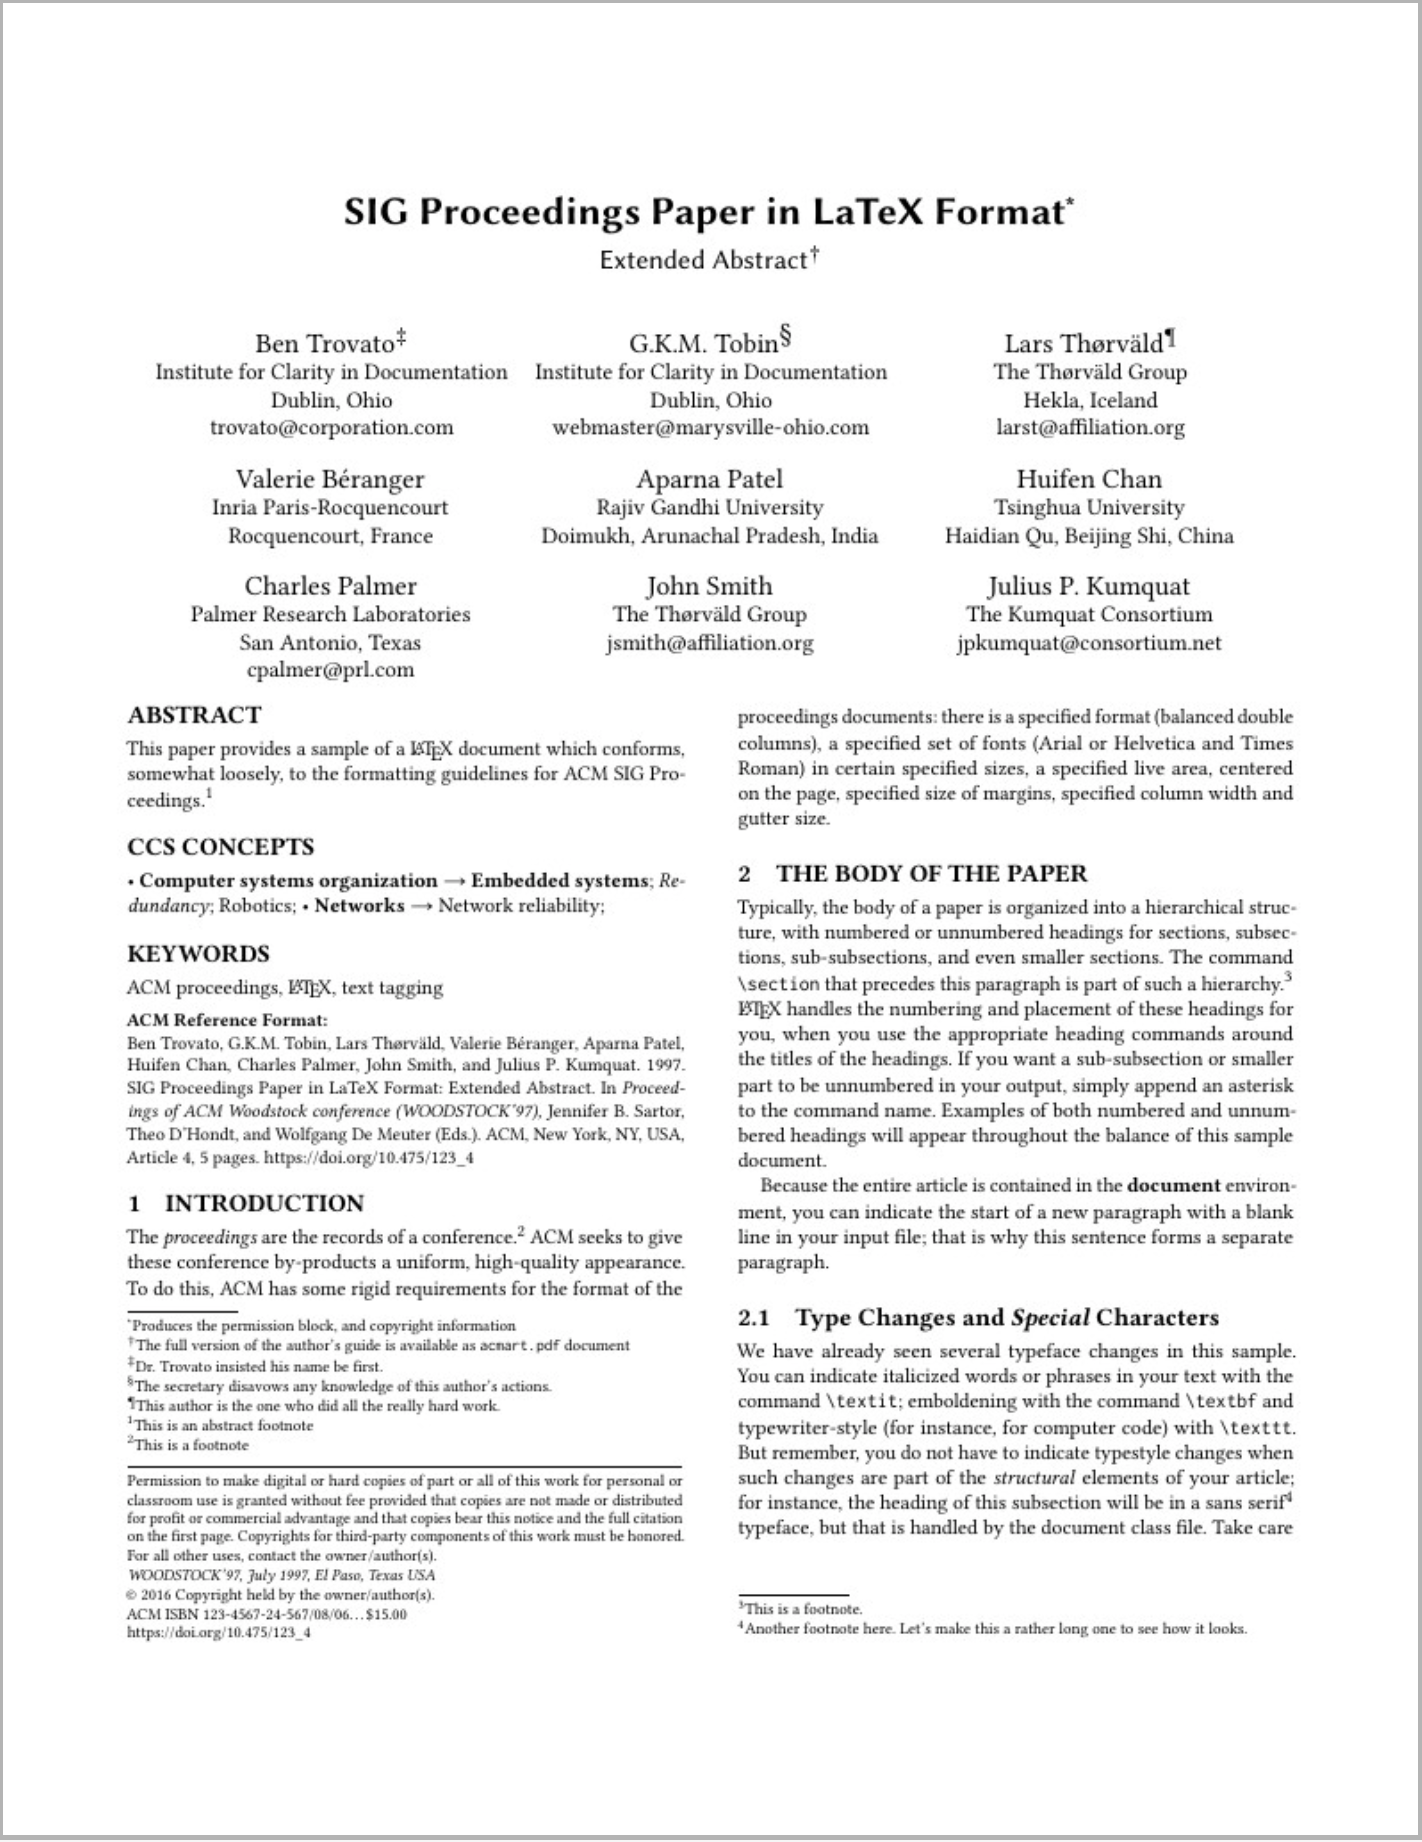
\includegraphics[width=6cm]{images/doc/acm.png}
  \hfill
  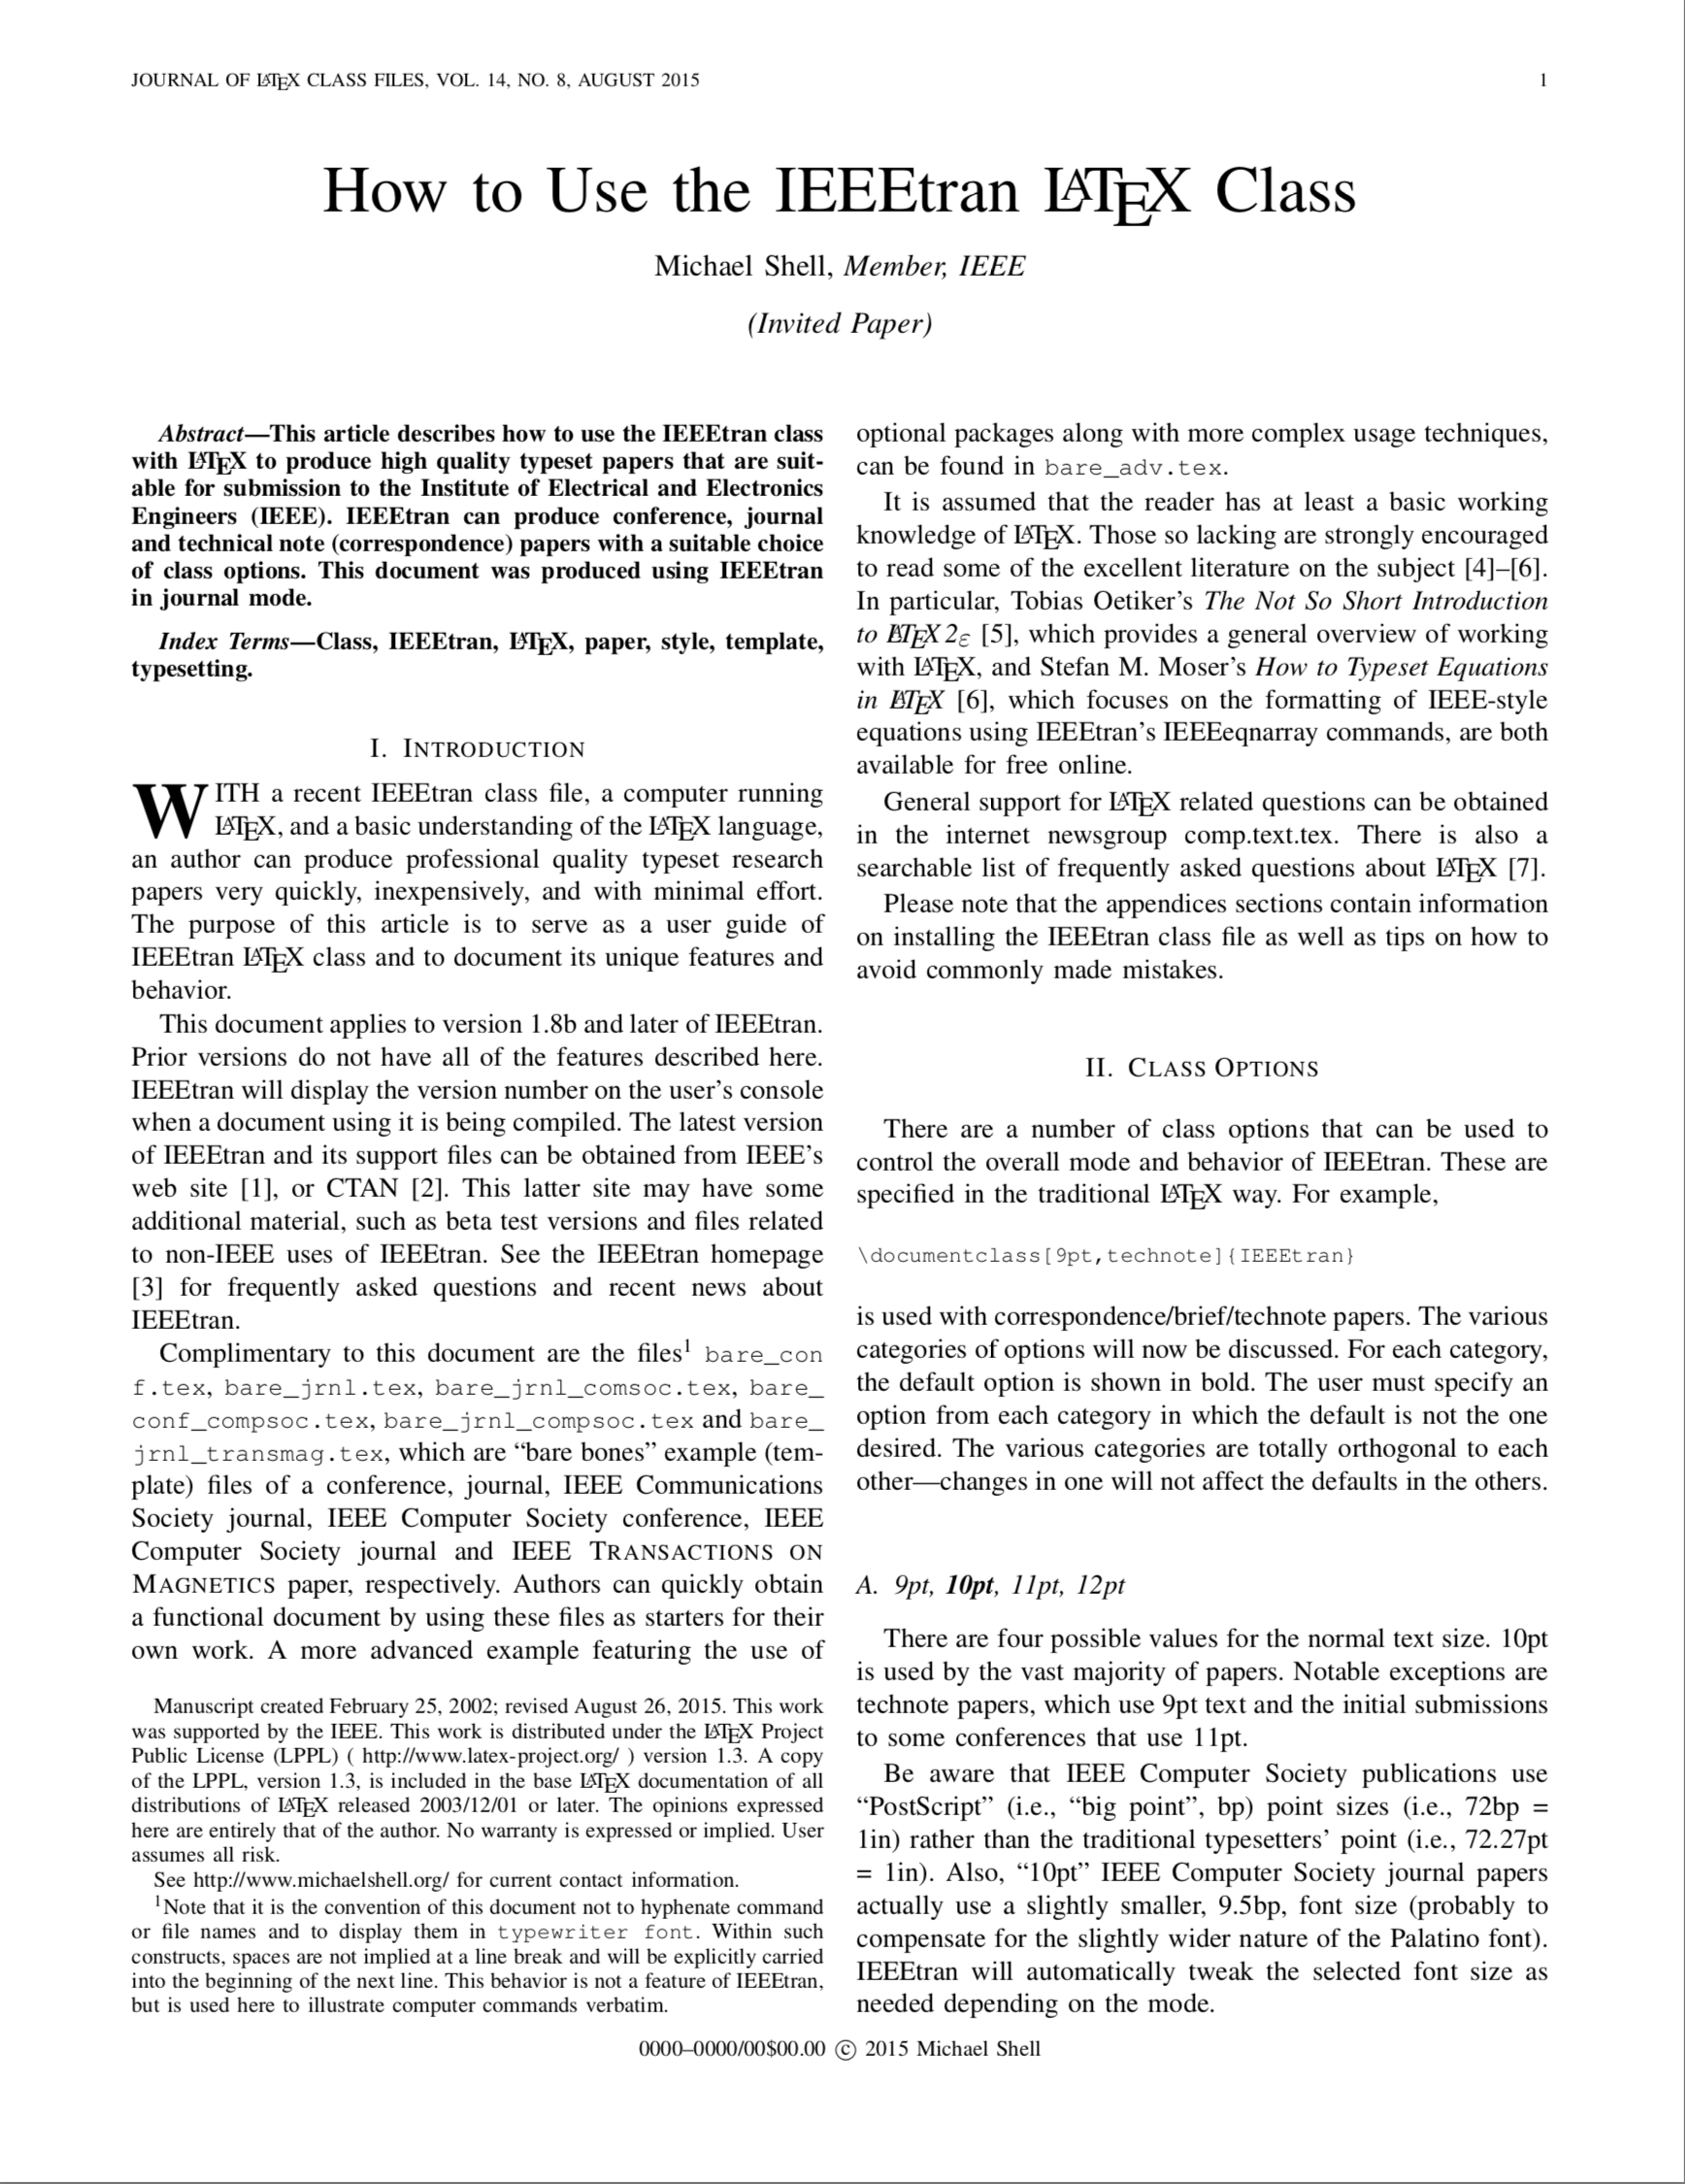
\includegraphics[width=6cm]{images/doc/ieee.png}
\caption{The look of the ACM and IEEE format templates}
\end{figure}

\begin{itemize}

\item
  \url{http://www.acm.org/publications/proceedings-template}
\item
  \url{https://www.ieee.org/conferences_events/conferences/publishing/templates.html}
\end{itemize}

\subsection{Generating and Managing Images}\label{generating-images}

To produce high quality images the programs PowerPoint and omnigraffle
on OSX are recommended. When using powerpoint please keep the image
ratio to 4x3 as they produce nice size graphics which you also can use
in your presentations. When using other rations they may not fit in
presentations and thus you may increase unnecessarily your work. We do
not recommend vizio as it is not universally available and produces
images that in case you have to present them in a slide presentation
does not easily reformat if you do not use 4x3 aspect ratio.

Naturally, graphics should be provided in SVG or PDF format so they can
scale well when we look at the final PDF. Including PNG, gif, or jpeg
files often do not result in the necessary resolution or the files
become real big. For this reason we for example can also not recommend
tools such as tablaeu as they do not provide proper exports to high
quality publication formats. For interactive display such tool may be
good, but for publications it produces inferior formatted images.

We recommend that all images be stored into a folder called images in
the same directory where your \LaTeX~ main document resides.



\subsection{Colored Boxes}

The package \verb|tcolorbox| provides sophisticated support to include
color boxes. Together with the new environment we can create nice add
ons to for example include notes.

\URL{http://osl.ugr.es/CTAN/macros/latex/contrib/tcolorbox/tcolorbox.pdf}

We have provided in this document notes as follows


\begin{tcblisting}{colback=blue!5!white,colframe=gray!50!blue,listing side text,  title=Note,fonttitle=\bfseries}
\begin{NOTE}
This is a note
\end{NOTE}
\end{tcblisting}

\begin{tcblisting}{colback=blue!5!white,colframe=gray!50!blue,listing side text,  title=Warning,fonttitle=\bfseries}
\begin{WARNING}
This is a note
\end{WARNING}
\end{tcblisting}


\subsection{Slides}\label{slides}
\index{Latex!slides}

Slides are best produced with the seminar package:

\begin{verbatim}
\documentclass{seminar}

\begin{slide}

    Hello World on slide 1

\end{slide}

The text between slides is ignored

\begin{slide}

    Hello World on slide 2

\end{slide}
\end{verbatim}

However, in case you need to have a slide presentation we recommend you
use ppt. Just paste and copy content from your PDF or your LaTeX source
file into the ppt.



\subsection{LaTeX vs. X}\label{latex-vs.-x}

We will refrain from providing a detailed analysis on why we use LaTeX
in many cases versus other technologies. In general, we find that LaTeX:

\begin{itemize}

\item
  is incredibly stable
\item
  produces high-quality output
\item
  is platform independent
\item
  has lots of templates
\item
  has been around for many years so it works well
\item
  removes you from the pain of figure placements
\item
  focusses you on content rather tan the appearance of the paper
\item
  integrates well with code repositories such as git to write
  collaborative papers.
\item
  has superior bibliography integration
\item
  has a rich set of tools that make using LaTeX easier
\item
  authors do not play with layouts much so papers in a format are
  uniform
\end{itemize}

In case you need a graphical view to edit LaTeX or LateX exportable
files you also find AucTeX and Lyx.

\subsubsection{Word}\label{word}

Word is arguably available to many, but if you work on Linux you may be
out of luck. Also Word often focusses not on structure of the text but
on its appearance. Many students abuse Word and the documents in Word
become a pain to edit with multiple users. Recently Microsoft has
offered online services to collaborate on writing documents in groups
which work well. Integration with bibliography managers such as endnote
or Mendeley is possible.

However, we ran into issues whenever we use word:

\begin{itemize}

\item
  Word tends sometimes to crash for unknown reasons and we lost a lot of
  work
\item
  Word has some issues with the bibliography managers and tends to crash
  sometimes for unknown reasons.
\item
  Word is slow with integration to large bibliographies.
\item
  Figure placement in Word in some formats is a disaster and you will
  spend many hours to correct things just to find out that if you make
  small changes you have to spend additional many hours to get used to
  the new placement. We have not yet experienced a word version where we
  have not lost images. Maybe that has changed, so let us know
\end{itemize}

However, we highly recommend the collaborative editing features of Word
that work on a paragraph and not letter level. Thus saving is essential
so you do not block other people from editing the paragraph.

\subsubsection{Google Docs}\label{google-docs}

Unfortunately, many useful features got lost in the new google docs.
However, it is great to collaborate quickly online, share thoughts and
even write your latex documents together if you like (just copy your
work in a file offline and use latex to compile it ;-) )

The biggest issue we have with Google Docs is that it does not allow the
support of 2 column formats, that the bibliography integration is
non-existent and that paste and copy from web pages and images
encourages unintended plagiarism when collecting information without
annotations (LaTeX and Word are prone to this too, but we found from
experience that it tends to happen more with Google docs users.

\subsubsection{A Place for Each}\label{a-place-for-each}

When looking at the tools we find a place for each:

\begin{description}
\item[Google docs:]
Short meeting notes, small documents, quick online collaborations to
develop documents collaboratively at the same time.
\item[Word:]
Available to many, supports 2 column format, supports paragraph based
collaborative editing, Integrates with bibliography managers.
\item[LaTeX:]
Reduces failures, great offline editing, superior bibliography
management, superior image placement, runs everywhere. Great
collaborative editing with sharelatex, allows easy generation of
proceedings written by hundreds of people with shared index.
\item[The best choice for your class:]
LaTeX
\end{description}

\section{Editing}\label{editing}

\subsection{Emacs}\label{emacs}

The text editor emacs provides a great basis for editing TeX and LaTeX
documents. Both modes are supported. In addition there exists a color
highlight module enabling the color display of LaTeX and TeX commands.
On OSX aquaemacs and carbon emacs have build in support for LaTeX. Spell
checking is done with flyspell in emacs.

\subsubsection{Aquamacs}

Aquamacs is an editor based on GNU Emacs that runs on OSX and
integrates with the OSX desktop. This is for many the preferred editor
on OSX for \LaTeX.

\url{http://aquamacs.org}

\begin{figure}[!htb]
  \centering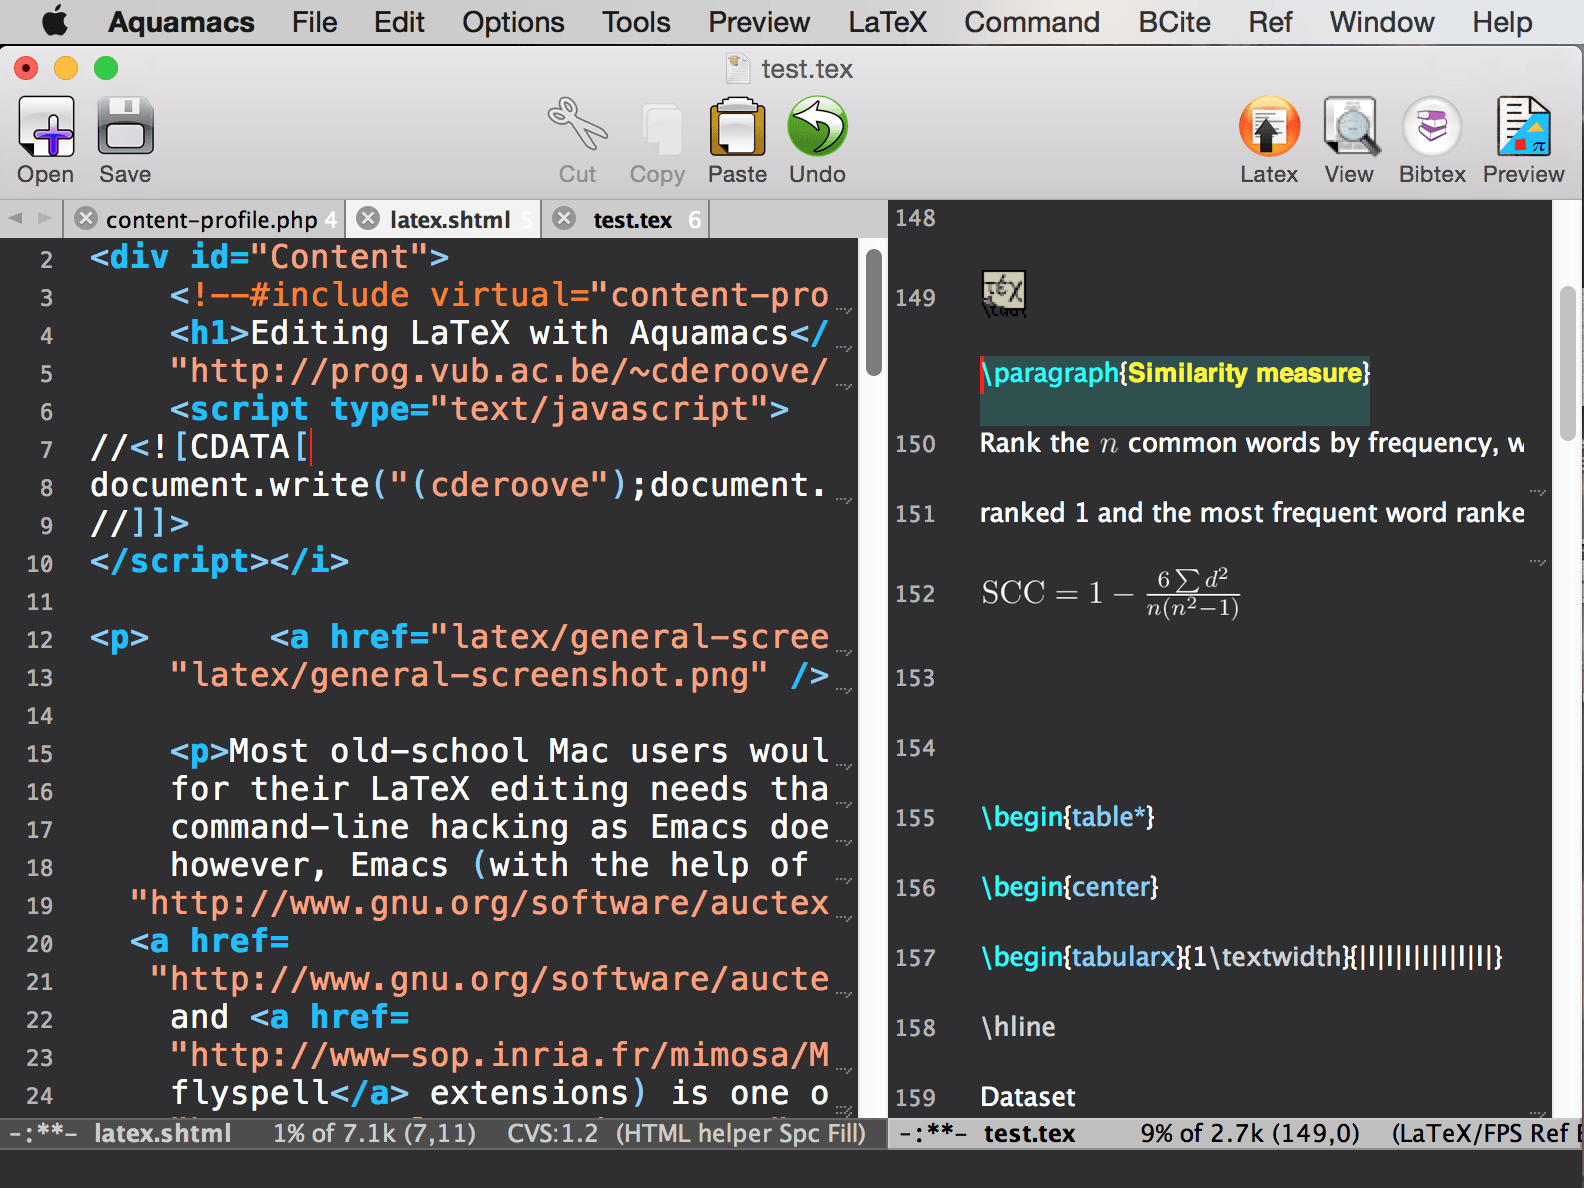
\includegraphics[width=8cm]{images/aquamacs.png}
  \caption{Aquamacs}
  \label{F:aquamacs}
\end{figure}


\subsection{Vi/Vim}\label{vivim}

Another popular editor is vi or vim. It is less feature rich but many
programmers ar using it. As it can edit ASCII text you can edit LaTeX.
With the LaTeX add-ons to vim, vim becomes similar powerful while
offering help and syntax highlighting for LaTeX as emacs does. (The
authors still prefer emacs)

\subsection{TeXshop}\label{texshop}

Other editors such as TeXshop are available which provide a more
integrated experience. However, we find them at times to stringent and
prefer editors such as emacs.

\subsection{LyX}\label{lyx}

We have made very good experiences with Lyx. You must assure that the
team you work with uses it consistently and that you all use the same
version.

\begin{figure}[!htb]
  \centering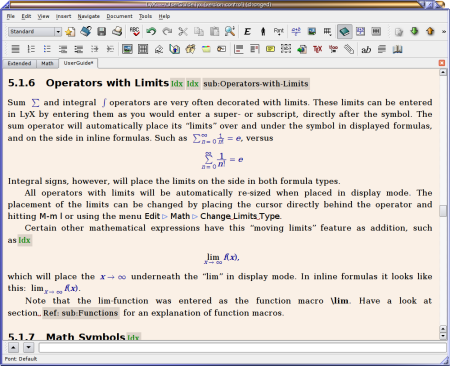
\includegraphics[width=8cm]{images/lyx.png}
  \caption{Lyx}
  \label{F:lyx}
\end{figure}

Using the ACM templates is documented here:

\begin{itemize}

\item
  \url{https://wiki.lyx.org/Examples/AcmSiggraph}
\end{itemize}

On OSX it is important that you have a new version of LaTeX and Lyx
installed. As it takes up quite some space, you ma want to delete older
versions. The new version of LyX comes with the acmsigplan template
included. However on OSX and other platforms the .cls file is not
included by default. However the above link clearly documents how to fix
this.

\subsection{WYSIWYG locally}\label{wysiwyg-locally}

We have found that editors such as Lyx and Auctex provide very good
WYSIWYG alike features. However, we found an even easier way while using
skim, a pdf previewer, in conjunction with emacs and latexmk. This can
be achieved while using the following command assuming your latex file
is called `report.tex`:

\begin{verbatim}
latexmk -pvc -view=pdf report
\end{verbatim}

This command will update your pdf previewer (make sure to use skim)
whenever you edit the file report.tex and save it. It will maintain via
skim the current position, thus you have a real great way of editing in
one window, while seeing the results in the other.

Skim can be found at: \url{http://skim-app.sourceforge.net/}

\subsection{Markdown and \LaTeX}
\index{Latex!markdown}

It may come as a surprise to many that one can actually write simple
LaTeX documents also in markdown Syntax or mix section written in
markdown while others are written in LaTeX. To do so all you ahve to
do is place the markdown text in a separate file. Let us call the file 
\verb|content.md| which has the following lines included in it:

\begin{verbatim}
# Section

* item a
* item b
\end{verbatim}

Obviously, we would have to convert this to LaTeX. Luckily there is a
very useful program called \textit{pandoc} that does this for you. YOu
could make the translation in the shell, but you could also make the
translation locally on your computer while allowing \LaTeX~ to start up
external programs. This is achieved with the \textit{write18} command and
allowing LaTeX explicitly to call external programs. Please inspect
the following latex file that includes a template on how to do
this. We assume the file is called markdown.tex for our example.

\begin{verbatim}
\documentclass{article}

\include{graphicx}
\newcommand{\tightlist}{}

\begin{document}
\immediate\write18{pandoc content.md -o content.tex}

\input{content}

\end{document}
\end{verbatim}

Now to generate the PDF we simply have to call the following command
that include the \textit{-shell-escape} flag to allow the execution of
write18 embedded commands:

\begin{verbatim}
pdflatex -shell-escape markdown-test
\end{verbatim}

The output will be \textit{markdown.pdf} with the content from the
markdown file translated. Doing this naturally allows you to write
large portions in markdown and automatically include them in your
LaTeX document. Hence, you can use editors such as Macdown to initially
work in semi WYSIWYG mode and do fairly straight forward
edition. Naturally the same can be done in RST. Naturally the most
elementary features are supported. For more sophisticated features,
please use LaTeX directly.


\subsection{Including RST into LaTeX}

content.rst:

\begin{verbatim}
Section
-------

* item a
* item b
\end{verbatim}

sample.tex:

\begin{verbatim}
\documentclass{article}

\include{graphicx}
\newcommand{\tightlist}{}

\begin{document}
\immediate\write18{pandoc content.rst -o content.tex}

\input{content}

\end{document}
\end{verbatim}


\subsection{pyCharm}

TODO: comment on how we can use pycharm for editing and what the
limitations are.

\subsection{MSWord}

it is possible to use Word.

be careful with 

\section{The LaTeX Cycle}\label{the-latex-cycle}
\index{Latex!cycle}

To create a PDF file from latex yo need to generate it following a
simple development and improvement cycle.

First, Create/edit ASCII source file with \texttt{file.tex} file:

\begin{verbatim}
emacs file.tex
\end{verbatim}

Create/edit bibliography file:

\begin{verbatim}
jabref refs.bib
\end{verbatim}

Create the PDF:

\begin{verbatim}
pdflatex file
bibtex file
pdflatex file
pdflatex file
\end{verbatim}

View the PDF:

\begin{verbatim}
open file
\end{verbatim}

It not only showcases you an example file in ACM 2 column format, but
also integrates with a bibliography. Furthermore, it provides a sample
Makefile that you can use to generate view and recompile, or even
autogenerate. A compilation would look like:

\begin{verbatim}
make
make view
\end{verbatim}

If however you want to do things on change in the tex file you can do
this automatically simply with:

\begin{verbatim}
make watch
\end{verbatim}

for make watch its best to use skim as pdf previewer


\section{Tips}\label{tips}

Including figures over two columns:

\begin{itemize}
\item
  \url{http://tex.stackexchange.com/questions/30985/displaying-a-wide-figure-in-a-two-column-document}
\item
  positioning figures with textwidth and columnwidth
  \url{https://www.sharelatex.com/learn/Positioning_images_and_tables}
\item
  An organization as the author. Assume the author is National Institute
  of Health and want to have the author show up, please do:

\begin{verbatim}
key= {National Institute of Health},
author= {{National Institute of Health}},
\end{verbatim}

  Please note the \{\{ \}\}
\item
  words containing `fi' or `ffi' showing blank places like below after
  recompiling it: find as nd efficiency as e ciency

  You copied from word or PDF ff which is actually not an ff, but a
  condensed character, change it to ff and ffi, you may find other such
  examples such as any non ASCII character. A degree is for example
  another common issue in data science.
\item
  do not use \textbar{} \& and other latex characters in bibtex
  references, instead use , and the word and
\item
  If you need to use \_ it is \_ but if you use urls leave them as is
\item
  We do recommend that you use sharelatex and jabref for writing papers.
  This is the easiest solution and beats in many cases MSWord as you can
  focus on writing and not on formatting.
\end{itemize}

\subsection{Colorful Output}

Instead of using pdflatex, you can also install \verb|pydflatex| that
provides a convenient wrapper and colorizes the output while
eliminating a lot of warnings that you may initially not want to deal
with. To install it please use:

\begin{verbatim}
pip install blessings
pip install -e "git+https://github.com/olivierverdier/pydflatex#egg=pydflatex"
\end{verbatim}

You can see the manual page with 

\begin{verbatim}
pydflatex --help

usage: usage: pydflatex [options] texfile1

Compile a tex file with pdflatex and make the auxiliary files invisible. Note
that the '.tex' extension may be omitted

positional arguments:
  tex path            path to tex file

optional arguments:
  -h, --help          show this help message and exit
  -o, --open          view the pdf file(s) in a pdf viewer.
  -k, --continue      continue on error
  -w, --with-warning  do not suppress common warnings
  -v, --verbose       Verbose output for debugging
  -p, --plain         No coloured output
  -x, --xetex         Use XeLaTeX engine
  -l, --log-parsing   Only parse log
  -t, --typesetting   Only typeset
\end{verbatim}

\subsection{latex2html}

\LaTeX~ can be exported to html with the the tool
\verb|latex2html|. It is available 

for Linux and OSX. More information can be found at

\URL{http://mirrors.ctan.org/support/latex2html/manual.pdf}

\URL{www.latex2html.org}

\begin{WARNING}
At this time the inastallation via brew install of latex2html is
broken. Instead one needs to conduct the insalation from source.

\begin{verbatim}
brew install latex2html
\end{verbatim}
\end{WARNING} 

The instalation from source can be conducted as follows

\begin{verbatim}
brew install libpng
wget https://github.com/latex2html/latex2html/archive/master.zip
uzip master.zip 
cd latex2html-master/
configure
make
make check
sudo make install
\end{verbatim}

\subsection{lachek}
\label{s:lacheck}
\index{lacheck}
\index{\LaTeX!lacheck}

Lacheck allows to find­ing common mistakes in \LaTeX~
documents. We recommend that you use it to check your latex files.

You can invoke it as follows

\begin{lstlisting}
lacheck filename.tex
\end{lstlisting}

More information can be found at

\URL{https://ctan.org/tex-archive/support/lacheck}

\subsection{chktex}
\label{s:chktex}
\index{chktex}
\index{\LaTeX!chktex}

LaTeX is a powerfull program to develop professional documents. In
some cases i is useful to check some semantics on the document. For
this reason you can use 

\begin{lstlisting}
chktex filename.tex
\end{lstlisting}

It will execute a number of filters and produce a check on them. You
can configure it to produce warnings and errors based on the error
type.

For a manual page use

\begin{lstlisting}
chktex --help
\end{lstlisting}

When using it some errors and wrnings can be ignored, while others
should be considerd. Supported featured mantiond on the Web page
include:
``
\begin{itemize}
          \item  Commands terminated with space. Ignores \verb|\tt|, etc.
          \item  Space in front of references instead of \verb|~|.
          \item  Forgetting to group parenthesis characters when
            sub-/superscripting.
          \item  Italic correction (\verb|\/|) mistakes (double, missing,
            unnecessary).
          \item  Parenthesis and environment matching.
          \item  Ellipsis detection; also checks whether to use \verb|\dots|,
            \verb|\cdots| or \verb|\ldots|.
          \item  Enforcement of normal space after abbreviation. Detects most
            abbreviations automagically.
          \item  Enforcement of end-of-sentence space when the last sentence
            ended with capital letter.
          \item  Math-mode on/off detection.
          \item  Quote checking, both wrong types (\verb|"|) and wrong direction.
          \item  Recommends splitting three quotes in a row.
          \item  Searching for user patterns.
          \item  Displays comments.
          \item  Space in front of \verb|\label| and similar commands.
          \item  Use of \verb|x| instead of \verb|$\times$| between numbers.
          \item  Multiple spaces in input which will be rendered as one space
            (or multiple spaces, where that is undesirable).
          \item  Warns about text which may be ignored.
          \item  Mathematical operators typeset as variables.
          \item  No space in front of/after parenthesis.
          \item  Demands a consistent quote style.
          \item  Punctuation inside inner math mode/outside display math mode.
          \item  Use of TeX primitives where LaTeX equivalents are available.
          \item  Space in front of footnotes.
          \item  Bogus characters following commands.
\end{itemize}
``

For more details see

\URL{http://baruch.ev-en.org/proj/chktex/}

\subsection{References}
\index{Latex!other documentation}

\begin{description}


\item[Latex Sheet:]    \url{https://wch.github.io/latexsheet/latexsheet.pdf}

\item[Latex Short:]    \url{http://tug.ctan.org/info/lshort/english/lshort.pdf}

\item[Wikibook:]       \url{https://en.wikibooks.org/wiki/LaTeX}
\item[Wikibook (PDF)]: \url{https://upload.wikimedia.org/wikipedia/commons/2/2d/LaTeX.pdf}

\item [Links to books:] \url{https://latexforhumans.wordpress.com/2008/10/11/the-best-guides-to-latex/}
\item [Links to books:] \url{https://www.latex-project.org/help/books/}
\item [LaTeX2e:]
  The
  \href{http://texdoc.net/texmf-dist/doc/latex/latex2e-help-texinfo/latex2e.pdf}{LaTeX
  Reference Manual} provides a good introduction to Latex.

\end{description}


\begin{itemize}

\item
  LaTeX Users and Reference Guide, by Leslie Lamport
  \url{https://www.amazon.com/LaTeX-Document-Preparation-System-2nd/dp/0201529831/ref=sr_1_2?s=books\&ie=UTF8\&qid=1507114870\&sr=1-2\&keywords=lamport}
\item
  LaTeX an Introduction, by Helmut Kopka
  \url{https://www.amazon.com/Guide-LaTeX-4th-Helmut-Kopka/dp/0321173856/ref=pd_lpo_sbs_14_t_0?_encoding=UTF8\&psc=1\&refRID=2BB4APDFEX34A4JM65ZB}
\item
  The LaTeX Companion, by Frank Mittelbach
  \url{https://www.amazon.com/LaTeX-Companion-Techniques-Computer-Typesetting/dp/0201362996}
\end{itemize}



\chapter{Managing Bibliographies}
\label{C:bibtex}

\FILENAME

\section{Integrating Bibliographies}
\label{S:bibliographies}
\index{Bibliography}
\index{bibtex}
\index{biber}

Bibliography management in \LaTeX\ is one of the many features that
motivate many researchers to make \LaTeX the tool of choice to write
academic papers. There are numerous bibliography styles available that
allow easy adaptation to differen journal and proceedings style. As
such, it includes styles for bibliographies formated in ACM and IEEE
style.

\subsection{biber}

\TODO{Describe use of biber instead of bibtex}

\subsection{bibtex}

This section assumes we use the standard bibtex program to integrate
citations into a \LaTeX\ paper.

An example to use the IEEE style for a paper includes to set
the style to IEEEtran before you add the reference:

\begin{verbatim}
\bibliographystyle{IEEEtran}
\bibliography{references.bib}
\end{verbatim}

To properly create PDF papers which using bibtex, we have to make sure
that all indexes, citations, references and labels are updated. This
is done with the help of the following commands assuming your file is
called \verb|file.tex|

\begin{verbatim}
pdflatex  file
bibtex file
pdflatex  file
pdflatex  file
\end{verbatim}


\begin{IU}
At IU you are required to use our template. which includes a Makefile
and either calls the above three commands or used latexmk
\end{IU}

The reason for the multiple execution of the latex program is to update
all cross-references correctly. In case you are not interested in
updating the library every time in the writing progress just postpone it
till the end. Missing citations are viewed as {[}?{]}.

Two programs stand out when managing bibliographies: emacs and jabref:

  \URL{http://www.jabref.org/}

Other programs such as Mendeley, Zotero, and even endnote integrate with
bibtex. However their support is limited, so we recommend that you just
use jabref as it is free and runs on all platforms.

\subsection{jabref}\label{jabref}

\TODO{Tyler: include cite for jabref, bibtex, biber at appropriate
  location in this section. Add them to the bib file.}

Practical experience with many generations of students shows that
\textit{jabref} is a very simple to use bibliography manager for LaTeX and
other systems. It can create a multitude of bibliography file formats
and allows upload in other online bibliography managers.

For information on how to install and use jabref please go to 
\url{http://www.jabref.org/}. There you will find the appropriate
download link.

We provide also a convenient video on how to use jabref and show
several methods on how to add entries easily to your bibliography database.

\video{Bibliography}{1:41}{jabref}{https://youtu.be/QVbifcLgMic}



\section{Entry types}

In this section we will explain how to find and properly generate
bibliographic entries. We are using bibtex for this as it is easy to
use and generates reasonable entries that can be included in
papers. What we like to achieve in this section is not to just show
you a final entry, but to document the process on how that entry was
derived. This will allow you to replicate or learn from the process to
apply to your own entries. As part of this we copy and paste
information found via Web searches.

We will address a number of important reference types which includes:

\begin{itemize}

\item
  wikipedia entries
\item
  github (see Section~\ref{s:e:source-code-references})
\item
  books
\item
  articles in a scientific journal (see Section~\ref{s:e:article-in-a-journal})
\item
  articles in a conference (see Section~\ref{s:e:article-in-a-conference-proceedings})
\item
  articles in magazines (non scientific)
\item
  blogs
\end{itemize}

\subsection{Source Code References}
\label{s:e:source-code-references}
\index{Bibtex!Source code}

Often, we need to cite a source code from a publicly hosted
repository. Such repositories are frequently used and include, for
example github, bitbucket, sourceforge, or your Universities code
repository as long as it is publicly reachable. As changes can occur on
these repositories, it is important that the date of access is listed in
the entry or even the release version of the source code.

Let us without bias chose a random source dode entry that has been
contributed by a student as follows:

\begin{verbatim}
@Misc{gonzalez_2015,
  Title =  {Buildstep},
  Author =     {Gonzalez, Jose and Lindsay, Jeff},
  HowPublished = {Web Page},
  Month =  {Jul},
  Note =   {Accessed: 2017-1-24},
  Year =   2015,
  Key =        {www-buildstep},
  Url =        {https://github.com/progrium/buildstep}
}
\end{verbatim}

Is this entry correct? Let us analyse. But first we need to undersrand
the semantics of the fields.

\subsubsection{What are the Different entry Types and Fields}

You see that the entry contains a number of fields. An extensive
explanation of these fields can be found at 

Please see \url{https://en.wikipedia.org/wiki/BibTeX}

We provide for this example a comprehensive discussions of the fields
used. For other examples we suggest you refer to the document to
identify what needs to be filled out.

\subsubsection{Entry type Misc}\label{s:e:entry-type-misc}
\index{Bibtex!Field!Misc}

First, it seems appropriate to use a \emph{@misc} entry. We correctly
identify this is a misc entry as it is online available. More recent
version of bibtex include also the type \emph{@online} for it. However,
in order to maintain compatibility to older formats we chose simply Misc
here and if we really would need to we could replace it easily.

\subsubsection{Label}\label{s:e:label}
\index{Bibtex!Field!Label}

Typically the bibliography label should contain 3 letters from an
author name, short year and the short name of the publication to
provide maximum information regarding the publication. However in this
case the project is hosted on github, so creating the label based on
just the github location seems more logical. Thus our label that we
propose is given by 

\verb|github-progrium-buildstep|


Under no circumstances should you use underscores as they can have unintended
consequences in programs we use to create papers for our classes. Just
use a minus sign instead. As it is hosted on github we also want the
githubname and the projectname. As you can see we just derived it from
the URL.

\begin{IU}
When managing bibliography entries with large numbers of collaborators
it is advisable that all bibliography labels be initially be prefixed
with an id for the collaborator. In our case we use the HID. Thus in
our case we will have the following label.

\verb|hid-sp18-000-github-progrium-buildstep|

\end{IU}


\subsubsection{Author}\label{s:e:author}
\index{Bibtex!Field!Author}

Normally we can write in the author fiels the names of the authors
separated by the work and. IT is important tu use the word \verb|and|
but not use a comma. However, this only works if the lastname does not
contain a space in it. In order to avoid confusing the system, we
recommend therefore to write all names in the form
\verb|Lastname, Firstname Middle Initials|

Thus we find in our example

\verb|  Author =     {Gonzalez, Jose and Lindsay, Jeff},|

\begin{WARNING}
Please note the word and between authors. and not a comma, commas are
only used to distinguish between lastname and firstname.
\end{WARNING}


\subsubsection{Key}\label{s:e:key}
\index{Bibtex!Field!Key}

In this case the key field can be removed as the entry has an author
field entry. If there was no author field, we use the key to specify
the alphabetical ordering based on the specified key. Note that a key is
not the label. In fact in our original entry the key field was wrongly
used and the student did not understand that the key is used for
sorting.

\subsubsection{Howpublished}\label{s:e:howpublished}
\index{Bibtex!Field!Howpublished}

Since the source is a github project repository, the howpublished field
shall hold the value \verb|{Code Repository}|. If the
url specified was a normal webpage, the \verb|{Web Page}| entry would be
valid.

\subsubsection{Month}\label{s:e:month}
\index{Bibtex!Field!Month}

To allow internationalization of the month we use the first 3 letters
in the english language for the month. Thus it is 
\verb|month = jul|. Note that there are no brackets around the month.

\subsubsection{Owner}\label{s:e:owner}
\index{Bibtex!Field!Owner}

In class we introduced the convention to put the student HID in it. If
multiple students contributed, add them with space separation.

\subsubsection{Accessed}\label{s:e:accessed}
\index{Bibtex!Field!Accessed}

As some styles do not support the accessed field, we simply include it in
the note field. This is absolutely essential as code can change and when
we read the code we looked at a particular snapshot in time. In addition
it is often necessary to record the actual version of the code or the branch.
Typically for github entries, it is best to just use the month and
year field as some styles check for it.

\subsubsection{Final Entry}

Filling out as many fields as possible with information for this entry
we get:

\begin{verbatim}
@Misc{github-progrium-buildstep,
  Title =  {Buildstep},
  Author =     {Jose Gonzalez and Jeff Lindsay},
  HowPublished = {Code Repository},
  Year =   {2015},
  Month =  jul,
  Note =   {Accessed: 2017-1-24, master branch},
  Url =    {https://github.com/progrium/buildstep},
  Owner =  {S17-IO-3025},
}
\end{verbatim}

We are using the release date in the year and month field as this
project uses this for organizing releases. However, other project may
have release versions so you would have in addition to using the data
also to include the version in the note field such as:

\begin{verbatim}
Note =     {Version: 1.2.3, Accessed: 2017-1-24},
\end{verbatim}


\subsection{Pedigree}

Often it is advantageous to document the pedigree of the bibtex
entries. Eg, how did you derive the final entry? To do so you can
simply add a field such as \verb|bibsource| and include in it all
links you used to gather the final entry. However, we believe that the
effort to curate an entry is sufficient to manage your own
bibliography which you should freely distribute and constitute an own
contribution. 

\subsection{Article in a Journal}
\label{s:e:article-in-a-journal}
\index{Bibtex!Article}

Many online bibtex entries that you will find are wrong or
incomplete. Often you may find via google a bibtex entry that may need
some more research. Let us assume your first google query returns a
publication and you cite it such as this:

\begin{verbatim}
@Unpublished{unpublished-google-sawzall,
    Title = {{Interpreting the Data: Parallel Analysis with Sawzall}},
    Author = {{Rob Pike, Sean Dorward, Robert Griesemer, Sean Quinlan}},
    Note = {accessed 2017-01-28},
    Month = {October},
    Year = {2005},
    Owner = {for the purpose of this discussion removed},
    Timestamp = {2017.01.31}
}
\end{verbatim}

Could we improve this entry to achieve your best? We observe:

\begin{enumerate}
\item
  The author field has a wrong entry as the , is to be replaced by an
  and.
\item
  The author field has authors and thus must not have a \{\{ \}\}
\item
  The url is missing, as the simple google search actually finds a PDF
  document.
\end{enumerate}

Let us investigate a bit more while searching for the title. We find

\begin{enumerate}
\def\labelenumi{\Alph{enumi})}
\item
  \url{https://www.google.com/url?sa=t\&rct=j\&q}=\&esrc=s\&source=web\&cd=1\&ved=0ahUKEwj\_ytSA-PDRAhUH8IMKHaomC-oQFggaMAA\&url=https\%3A\%2F\%2Fresearch.google.com\%2Farchive\%2Fsawzall-sciprog.pdf\&usg=AFQjCNHSSfKBwbxVAVPQ0td4rTjitKucpA\&sig2=vbiVzi36B3gGFjIzlUKBDA\&bvm=bv.146073913,d.amc
\item
  \url{https://research.google.com/pubs/pub61.html}
\item
  \url{http://dl.acm.org/citation.cfm?id=1239658}
\end{enumerate}

Let us look at A)

As you can see from the url this is actually some redirection to a google
web page which probably is replaced by B as its from google research. So
let us look at B)

Now when you look at the link we find the url
\url{https://research.google.com/archive/sawzall-sciprog.pdf} which
redirects you to the PDF paper.

When we go to B) we find surprisingly a bibtex entry as follows:

\begin{verbatim}
@article{61,
  title = {Interpreting the Data: Parallel Analysis with Sawzall},
  author = {Rob Pike and Sean Dorward and Robert Griesemer and Sean Quinlan},
  year = 2005,
  URL = {https://research.google.com/archive/sawzall.html},
  journal = {Scientific Programming Journal},
  pages = {277--298},
  volume = {13}
}
\end{verbatim}

Now we could say let us be satisfied, but C) seems to be even more
interesting as its from a major publisher. So lats just make sure we
look at C)

If you go to C, you find under the colored box entitled Tools and
Resources a link called \textbf{bibtex}. Thus it seems a good idea to
click on it. This will give you:

\begin{verbatim}
@article{Pike:2005:IDP:1239655.1239658,
    author = {Pike, Rob and Dorward, Sean and Griesemer, Robert and Quinlan, Sean},
    title = {Interpreting the Data: Parallel Analysis with Sawzall},
    journal = {Sci. Program.},
    issue_date = {October 2005},
    volume = {13},
    number = {4},
    month = oct,
    year = {2005},
    issn = {1058-9244},
    pages = {277--298},
    numpages = {22},
    url = {http://dx.doi.org/10.1155/2005/962135},
    doi = {10.1155/2005/962135},
    acmid = {1239658},
    publisher = {IOS Press},
    address = {Amsterdam, The Netherlands, The Netherlands},
}
\end{verbatim}

Now we seem to be at a position to combine our search result as neither
entry is sufficient. As the doi number properly specifies a paper (look
up what a doi is) we can replace the url with one that we find online,
such as the one we found in A) Next we see that all field sin B are
already covered in C, so we take C) and add the url. Now as the label is
great and uniform for ACM, but for us a bit less convenient as its
difficult to remember, we just change it while for example using
authors, title, and year information. let us also make sure to do mostly
lowercase in the label just as a convention. Thus our entry looks like:

\begin{verbatim}
@article{pike05swazall,
    author = {Pike, Rob and Dorward, Sean and Griesemer, Robert and Quinlan, Sean},
    title = {Interpreting the Data: Parallel Analysis with Sawzall},
    journal = {Sci. Program.},
    issue_date = {October 2005},
    volume = {13},
    number = {4},
    month = oct,
    year = {2005},
    issn = {1058-9244},
    pages = {277--298},
    numpages = {22},
    url = {https://research.google.com/archive/sawzall-sciprog.pdf},
    doi = {10.1155/2005/962135},
    acmid = {1239658},
    publisher = {IOS Press},
    address = {Amsterdam, The Netherlands, The Netherlands},
}
\end{verbatim}

As you can see properly specifying a reference takes multiple google
queries and merging of the results you find from various returns. As
you still have time to correct things I advise that you check your
references and correct them. If the original reference would have been
graded it would have been graded with a ``fail'' instead of a ``pass''.

Naturally you need to judge if you can integrate the URL or not, often
papers exist in a prepublication and you must make sure to cite the
version you used. IN fact if you have the prepublicAtion, you should
obtain the final manuscript as it could contain significant
corrections to the previous draft. In other cases the prepublication
may just be fine and you could for your own references keep the
url. FOr the final publication you probably want to make sure that the
doi is used. FOr the collection of your references, adding the url
could be useful.

\subsection{Article in a Conference Proceedings}
\label{s:e:article-in-a-conference-proceedings}
\index{Bibtex!InProceedings}

Now let us look at another obvious example that needs improvement:

\begin{verbatim}
@InProceedings{wettinger-any2api,
  Title      = {Any2API - Automated APIfication},
  Author     = {Wettinger, Johannes and
                Uwe Breitenb{\"u}cher
                and Frank Leymann},
  Booktitle  = {Proceedings of the 5th International
                Conference on Cloud Computing and
                Services Science},
  Year       = {2015},
  Pages      = {475­486},
  Publisher  = {SciTePress},
  ISSN       = {2326-7550},
  Owner      = {S17-IO-3005},
  Url        = {https://pdfs.semanticscholar.org/1cd4/4b87be8cf68ea5c4c642d38678a7b40a86de.pdf}
}
\end{verbatim}

As you can see this entry seems to define all required fields, so we
could be tempted to stop here. But its good to double check. Let us do
some queries against ACM and google scholar. Let us just type in the
title, and if this is in a proceedings they should return hopefully a
predefined bibtex record for us.

Let us query:

\begin{verbatim}
google: googlescholar Any2API Automated APIfication
\end{verbatim}

We get:

\begin{itemize}

\item
  \url{https://scholar.google.de/citations?view_op=view_citation\&hl=en\&user=j6lIXt0AAAAJ\&citation_for_view=j6lIXt0AAAAJ:8k81kl-MbHgC}
\end{itemize}

On that page we see
\href{https://scholar.google.com/scholar_lookup?title=Automated+drug+dispensing+system+reduces+medication+errors+in+an+intensive+care+setting\&author=Chapuis\&publication_year=2010\#}{Cite}

So we find a PDF at
\url{https://pdfs.semanticscholar.org/1cd4/4b87be8cf68ea5c4c642d38678a7b40a86de.pdf}

Let us click on this and the document includes a bibtex entry such as:

\begin{verbatim}
@inproceedings{Wettinger2015, 
  author= {Johannes Wettinger and Uwe Breitenb{\"u}cher and Frank
       Leymann},
  title = {Any2API - Automated APIfication},
  booktitle = {Proceedings of the 5th International Conference on Cloud
       Computing and Service Science (CLOSER)},
  year = {2015},
  pages = {475--486},
  publisher = {SciTePress}
} 
\end{verbatim}

Now let us add the URL and owner:

\begin{verbatim}
@inproceedings{Wettinger2015, 
  author= {Johannes Wettinger and Uwe Breitenb{\"u}cher and Frank
       Leymann},
  title = {Any2API - Automated APIfication},
  booktitle = {Proceedings of the 5th International Conference on Cloud
       Computing and Service Science (CLOSER)},
  year = {2015},
  pages = {475--486},
  publisher = {SciTePress},
  url ={https://pdfs.semanticscholar.org/1cd4/4b87be8cf68ea5c4c642d38678a7b40a86de.pdf},
  owner = {S17-IO-3005},
} 
\end{verbatim}

Should we be satisfied? No, even our original information we gathered
provided more information. So let us continue. Let us issue additional
google searches with ACM or IEEE and the title. When doing the IEEE in the
example we find an entry called

\href{http://dblp.uni-trier.de\%2Fpers\%2Fl\%2FLeymann\%3AFrank\&usg=AFQjCNHCu-66qxWH0zRlPLr4DA8jIo5V-g\&sig2=1vYdnGOEiMcLBEMpbeBA7g}{dlp:
Frank Leyman}

Let us look at it and we find two entries:

\begin{verbatim}
@inproceedings{DBLP:conf/closer/WettingerBL15,
  author    = {Johannes Wettinger and
       Uwe Breitenb{\"{u}}cher and
       Frank Leymann},
  title     = {{ANY2API} - Automated APIfication - Generating APIs for Executables
       to Ease their Integration and Orchestration for Cloud Application
       Deployment Automation},
  booktitle = {{CLOSER} 2015 - Proceedings of the 5th International Conference on
       Cloud Computing and Services Science, Lisbon, Portugal, 20-22 May,
       2015.},
  pages     = {475--486},
  year      = {2015},
  crossref  = {DBLP:conf/closer/2015},
  url       = {http://dx.doi.org/10.5220/0005472704750486},
  doi       = {10.5220/0005472704750486},
  timestamp = {Tue, 04 Aug 2015 09:28:21 +0200},
  biburl    = {http://dblp.uni-trier.de/rec/bib/conf/closer/WettingerBL15},
  bibsource = {dblp computer science bibliography, http://dblp.org}
}

@proceedings{DBLP:conf/closer/2015,
  editor    = {Markus Helfert and
       Donald Ferguson and
       V{\'{\i}}ctor M{\'{e}}ndez Mu{\-{n}}oz},
  title     = {{CLOSER 2015 - Proceedings of the 5th International Conference on
       Cloud Computing and Services Science, Lisbon, Portugal, 20-22 May,
       2015}},
  publisher = {SciTePress},
  year      = {2015},
  isbn      = {978-989-758-104-5},
  timestamp = {Tue, 04 Aug 2015 09:17:34 +0200},
  biburl    = {http://dblp.uni-trier.de/rec/bib/conf/closer/2015},
  bibsource = {dblp computer science bibliography, http://dblp.org}
}
\end{verbatim}

So let us look at the entry and see how to get a better one for our
purpose and combine them. When using jabref, you see optional and
required fields, we want to add as many as possible, regardless if
optional or required, so Let us do that (We write it here in ASCII as it
is easier to document and can also be done in emacs:

\begin{verbatim}
@InProceedings{,
  author =   {},
  title =    {},
  OPTcrossref =  {},
  OPTkey =   {},
  OPTbooktitle = {},
  OPTyear =      {},
  OPTeditor =    {},
  OPTvolume =    {},
  OPTnumber =    {},
  OPTseries =    {},
  OPTpages =     {},
  OPTmonth =     {},
  OPTaddress =   {},
  OPTorganization = {},
  OPTpublisher = {},
  OPTnote =      {},
  OPTannote =    {},
  url = {}
}
\end{verbatim}

Now we copy and fill out the \textbf{form} from our various searches:

\begin{verbatim}
@InProceedings{Wettinger2015any2api,    
  author    = {Johannes Wettinger and
     Uwe Breitenb{\"{u}}cher and
     Frank Leymann},
  title     = {{ANY2API - Automated APIfication - Generating APIs for Executables
     to Ease their Integration and Orchestration for Cloud Application
     Deployment Automation}},
  booktitle = {{CLOSER 2015 - Proceedings of the 5th International Conference on
       Cloud Computing and Services Science}},
  year =     {2015},
  editor    = {Markus Helfert and
       Donald Ferguson and
       V{\'{\i}}ctor M{\'{e}}ndez Mu{\-{n}}oz},
  publisher = {SciTePress},
  isbn      = {978-989-758-104-5},
  pages = {475--486},
  month = {20-22 May},
  address =      {Lisbon, Portugal},
  doi       = {10.5220/0005472704750486},
  url ={https://pdfs.semanticscholar.org/1cd4/4b87be8cf68ea5c4c642d38678a7b40a86de.pdf},
  owner = {S17-IO-3005},
}
\end{verbatim}


For the rest of the section we provide just some simple examples.

\subsection{InProceedings}\label{s:e:inproceedings}
\index{Bibtex!InProceedings}

Please fill out

\begin{verbatim}
@InProceedings{,
  author =       {},
  title =        {},
  OPTcrossref =  {},
  OPTkey =       {},
  OPTbooktitle = {},
  OPTyear =      {},
  OPTeditor =    {},
  OPTvolume =    {},
  OPTnumber =    {},
  OPTseries =    {},
  OPTpages =     {},
  OPTmonth =     {},
  OPTaddress =   {},
  OPTorganization = {},
  OPTpublisher = {},
  OPTnote =      {},
  OPTannote =    {},
  url = {}
}
\end{verbatim}

\begin{verbatim}
@inproceedings{vonLaszewski15tas,
  author =     {DeLeon, Robert L. and Furlani, Thomas R. and Gallo,
                  Steven M. and White, Joseph P. and Jones, Matthew
                  D. and Patra, Abani and Innus, Martins and Yearke,
                  Thomas and Palmer, Jeffrey T. and Sperhac, Jeanette
                  M. and Rathsam, Ryan and Simakov, Nikolay and von
                  Laszewski, Gregor and Wang, Fugang},
  title =  {{TAS View of XSEDE Users and Usage}},
  booktitle =  {Proceedings of the 2015 XSEDE Conference: Scientific
                  Advancements Enabled by Enhanced
                  Cyberinfrastructure},
  series =     {XSEDE '15},
  year =   2015,
  isbn =   {978-1-4503-3720-5},
  location =   {St. Louis, Missouri},
  pages =  {21:1--21:8},
  articleno =  21,
  numpages =   8,
  url =        {http://doi.acm.org/10.1145/2792745.2792766},
  doi =        {10.1145/2792745.2792766},
  acmid =  2792766,
  publisher =  {ACM},
  address =    {New York, NY, USA},
  keywords =   {HPC, SUPReMM, TAS, XDMoD, XSEDE usage, XSEDE users},
}
\end{verbatim}

\subsection{TechReport}\label{s:e:techreport}
\index{Bibtex!TechReport}

Please fill out

\begin{verbatim}
@TechReport{,
  author =       {},
  title =        {},
  institution =  {},
  year =         {},
  OPTkey =       {},
  OPTtype =      {},
  OPTnumber =    {},
  OPTaddress =   {},
  OPTmonth =     {},
  OPTnote =      {},
  OPTannote =    {},
  url = {}    
}
\end{verbatim}

\begin{verbatim}
@TechReport{las05exp,
  title =  {{The Java CoG Kit Experiment Manager}},
  Author =     {von Laszewski, Gregor},
  Institution =    {Argonne National Laboratory},
  Year =   2005,
  Month =  jun,
  Number =     {P1259},
  url = {https://laszewski.github.io/papers/vonLaszewski-exp.pdf}
}
\end{verbatim}

\subsection{Article}
\index{Bibtex!Article}

Please fill out

\begin{verbatim}
@Article{,
  author =       {},
  title =        {},
  journal =      {},
  year =         {},
  OPTkey =       {},
  OPTvolume =    {},
  OPTnumber =    {},
  OPTpages =     {},
  OPTmonth =     {},
  OPTnote =      {},
  OPTannote =    {},,
  url = {}
}
\end{verbatim}

\begin{verbatim}
@Article{las05gridhistory,
  title =  {{The Grid-Idea and Its Evolution}},
  author =     {von Laszewski, Gregor},
  journal =    {Journal of Information Technology},
  year =   2005,
  month =  jun,
  number =     6,
  pages =  {319-329},
  volume =     47,
  doi =        {10.1524/itit.2005.47.6.319},
  url = {https://laszewski.github.io/papers/vonLaszewski-grid-idea.pdf}
}
\end{verbatim}

\subsection{Proceedings}\label{s:e:proceedings}
\index{Bibtex!Proceedings}

Please fill out

\begin{verbatim}
@Proceedings{,
  title =        {},
  year =         {},
  OPTkey =       {},
  OPTbooktitle = {},
  OPTeditor =    {},
  OPTvolume =    {},
  OPTnumber =    {},
  OPTseries =    {},
  OPTaddress =   {},
  OPTmonth =     {},
  OPTorganization = {},
  OPTpublisher = {},
  OPTnote =      {},
  OPTannote =    {},
  url = {}
}
\end{verbatim}

\begin{verbatim}
@Proceedings{las12fedcloud-proc,
  title =  {{FederatedClouds '12: Proceedings of the 2012
                  Workshop on Cloud Services, Federation, and the 8th
                  Open Cirrus Summit}},
  year =   2012,
  address =    {New York, NY, USA},
  editor =     {vonLaszewski, Gregor and Robert Grossman and Michael
                  Kozuchand Rick McGeerand Dejan Milojicic},
  publisher =  {ACM},
  iSBN =   {978-1-4503-1754-2},
  location =   {San Jose, California, USA},
  url =
                  {http://dl.acm.org/citation.cfm?id=2378975&picked=prox&cfid=389635474&cftoken=32712991}
}
\end{verbatim}

\subsection{Wikipedia Entry}\label{s:e:wikipedia-entry}
\index{Bibtex!Wikipedia Entry}

Please fill out

\begin{verbatim}
@Misc{,
  OPTkey =       {},
  OPTauthor =    {},
  OPTtitle =     {},
  OPThowpublished = {},
  OPTmonth =     {},
  OPTyear =      {},
  OPTnote =      {},
  OPTannote =    {},
  url = {}
}
\end{verbatim}

\begin{verbatim}
@Misc{www-ode-wikipedia,
  Title =  {Apache ODE},
  HowPublished = {Web Page},
  Note =   {Accessed: 2017-2-11},
  Key =        {Apache ODE},
  Url =        {https://en.wikipedia.org/wiki/Apache_ODE}
}
\end{verbatim}

\subsection{Blogs}\label{blogs}
\index{Bibtex!Blog}

Please fill out

\begin{verbatim}
@Misc{,
  OPTkey =       {},
  OPTauthor =    {},
  OPTtitle =     {},
  OPThowpublished = {},
  OPTmonth =     {},
  OPTyear =      {},
  OPTnote =      {},
  OPTannote =    {},
  OPTurl = {}
}
\end{verbatim}

\begin{verbatim}
@Misc{www-clarridge-discoproject-blog,
  title =  {Disco - A Powerful Erlang and Python Map/Reduce
                  Framework},
  uthor =  {Clarridge, Tait},
  howpublished = {Blog},
  month =  may,
  note =   {Accessed: 25-feb-2017},
  year =   2014,
  url =  {http://www.taitclarridge.com/techlog/2014/05/disco-a-powerful-erlang-and-python-mapreduce-framework.html}
}
\end{verbatim}

\subsection{Web Page}\label{s:e:web-page}
\index{Bibtex!Web Page}

Please fill out

\begin{verbatim}
@Misc{, 
  OPTkey =       {}, 
  OPTauthor =    {}, 
  OPTtitle =     {}, 
  OPThowpublished = {}, 
  OPTmonth =     {}, 
  OPTyear =      {}, 
  OPTnote =      {},
  OPTannote =    {},
  url = {}
}
\end{verbatim}

\begin{verbatim}
@Misc{www-cloudmesh-classes,
  OPTkey =       {},
  author =    {von Laszewski, Gregor},
  title =     {Cloudmesh Classes},
  howpublished = {Web Page},
  OPTmonth =     {},
  OPTyear =      {},
  OPTnote =      {},
  OPTannote =    {},
  url = {https://cloudmesh.github.io/classes/}
}
\end{verbatim}

\begin{verbatim}
@Misc{www-awslambda,
  title =  {AWS Lambda},
  author =     {{Amazon}},
  key =        {AWS Lambda},
  howpublished = {Web Page},
  url =        {https://aws.amazon.com/lambda/faqs/}
}
\end{verbatim}

\subsection{Book}\label{s:e:book}
\index{Bibtex!book}

Given the following entry. What is the proper entry for this book.
Provide rationale:

\begin{verbatim}
@Book{netty-book,
    Title = {Netty in Action},
    Author = {Maurer, Norman and Wolfthal, Marvin},
    Publisher = {Manning Publications},
    Year = {2016},
}
\end{verbatim}

To obtain the record of a book you can look at many information sources.
The can include:

\begin{itemize}

\item
  \url{https://www.manning.com/books/netty-in-action}
\item
  \url{https://www.amazon.com/Netty-Action-Norman-Maurer/dp/1617291471}
\item
  \url{http://www.barnesandnoble.com/w/netty-in-action-norman-maurer/1117342155?ean=9781617291470\#productInfoTabs}
\item
  \url{http://www.powells.com/book/netty-in-action-9781617291470/1-0}
\end{itemize}

Furthermore, we need to consider the entry of a book, we simply look it
up in emacs where we find the following but add the owner and the url
field:

\begin{verbatim}
@Book{,
  ALTauthor =      {},
  ALTeditor =      {},
  title =      {},
  publisher =      {},
  year =   {},
  OPTkey =     {},
  OPTvolume =      {},
  OPTnumber =      {},
  OPTseries =      {},
  OPTaddress =     {},
  OPTedition =     {},
  OPTmonth =   {},
  OPTnote =    {},
  OPTannote =      {},
  ownwer =       {},
  url = {}
}
\end{verbatim}

In summary we find the following fields:

\begin{description}
\item[Required fields:]
author/editor, title, publisher, year
\item[Optional fields:]
volume/number, series, address, edition, month, note, key
\end{description}

We apply the following to fill out the fields which is the standard
definition as defined by \LaTeX.

\begin{description}
\item[address:]
The address is the Publisher's address. Usually just the city, but can
be the full address for lesser-known publishers.
\item[author:]
The name(s) of the author(s) (in the case of more than one author,
separated by and) Names can be written in one of two forms: Donald E.
Knuth or Knuth, Donald E. or van Halen, Eddie. Please note that Eddie
van Halen would result in a wrong name. For our purpose we keep nobelity
titles part of the last name.
\item[edition:]
The edition of a book, long form (such as ``First'' or ``Second'')
\item[editor:]
The name(s) of the editor(s)
\item[key:]
A hidden field used for specifying or overriding the alphabetical order
of entries (when the ``author'' and ``editor'' fields are missing). Note
that this is very different from the key that is used to cite or
cross-reference the entry.
\item[label:]
The label field should contain three letters from the auth field, a
short year reference and a short name of the publication to provide the
maximum information regarding the publication. Underscores should be
replaced with dashes or removed completely.
\item[month:]
The month of publication or, if unpublished, the month of creation. Use
three-letter abbreviations for this field in order to account for
languages that do not capitalize month names. Additional information for
the day can be included as follows: aug \#``\textasciitilde{}10,''
\item[publisher:]
The publisher's name
\item[series:]
The series of books the book was published in (e.g. ``The Hardy Boys''
or ``Lecture Notes in Computer Science'')
\item[title:]
The title of the work. As the capitalization depends on the bibliography
style and the language used we typically use camel case. To force
capitalization of a word or its first letter you can use the curly
braces, `\{ \}'. To keep the title in camel case simple use title =
\{\{My Title\}\}
\item[type:]
The field overriding the default type of publication (e.g. ``Research
Note'' for techreport, ``\{PhD\} dissertation'' for phdthesis,
``Section'' for inbook/incollection) volume The volume of a journal or
multi-volume book year The year of publication (or, if unpublished, the
year of creation)
\end{description}

While applying the above rules and tips we summarize what we have done
for this entry:

\begin{enumerate}
\def\labelenumi{\arabic{enumi}.}
\item
  Search for the book by title/Author on ACM (\url{http://dl.acm.org/})
  or Amazon or barnesandnoble or upcitemdb (\url{http://upcitemdb.com}).
  These services return bibtex entrie that you can improve.
\item
  Hence one option is t get the ISBN of the book. For ``Mesos in
  action'' from upcitemdb we got the ISBN as ``9781617 292927''. This is
  the 13 digit ISBN. The first 3 digits (GS1 code) can be skipped. Using
  the rest of 10 digits ``1617 292927'', Add in JabRef in Optional
  Fields-\textgreater{}ISBN.

  However it is fine to youst specify the full number.

  We can also return a bibtex entry generated while using Click on the
  ``Get BibTex from ISBN''.

  Now we get more information on this book entry from ISBN. We can opt
  either the original or newly searched entry for the below bibtex
  fields or merge as appropriate. URL may not match from where we
  initially read the book, however there is option to put your original
  url or newly searched url. EAN, Edition, Pages,url,published date etc.
  Do a search on amazon for ``ASIN''. Can skip if not available.
  Sometime we get ASIN for a different publication, maybe a paperback
  ASIN=\{B01MT311CU\} We can add it as it becomes easier to search
\end{enumerate}

\begin{description}
\item[doi:]
If you can find a doi numer you should also add it. IN this case we
could not locate one.
\end{description}

As a result we obtain the entry:

\begin{verbatim}
@Book{netty-book,
  title = {Netty in Action},
  publisher = {Manning Publications Co.},
  year = {2015},
  author = {Maurer, Norman and Wolfthal, Marvin Allen},
  address = {Greenwich, CT, USA},
  edition = {1st},
  isbn = {1617291471},
  asin = {1617291471},
  date = {2015-12-23},
  ean = {9781617291470},
  owner = {S17-IO-3022 S17-IO-3010 S17-IO-3012},
  pages = {296},
  url = {http://www.ebook.de/de/product/21687528/norman_maurer_netty_in_action.html},
}
\end{verbatim}

\section{Integrating Bibtex entries into Other Systems}

We have not tested any of this

\subsection{jabref and MSWord}
\index{Bibtex!MSWord}

According to others it is possible to integrate jabref references
directly into MSWord. 
For more information please see:
\URL{https://www.paulkiddie.com/2009/07/jabref-exports-to-word-2007-xml/}


\subsection{Bibtex import to MSWord}\label{bibtex-import-to-msword}

\subsubsection{XML import}
\index{Bibtex!MSWord}

Please give feedback if you used this.

see:
\URL{http://blog.pengyifan.com/using-bibtex-in-ms-word-2015-mac-os/}

\begin{enumerate}

\item  In JabRef, export the bibliography in MS Word 2008 xml format

\item  Name the file Sources.xml (case sensitive)
\item   In OSX with MS Word 2015: Go to
  \verb|/Library/Containers/com.microsoft.word/Data/Library/Application Support/Microsoft/Office.|
\item  Rename the original Sources.xml file to Sources.xml.bak
\item  Copy the generated Sources.xml in this folder
\item  Restart MS Word.

\end{enumerate}

We do not know what needs to be done in case you need to make changes to
the references. Please report back your experiences. To avoid issues we
recommend that you use LaTeX. and not MSWord.

\subsubsection{BibTex4Word}
\index{bibtex4word}

We have not tried this:

\URL{http://www.ee.ic.ac.uk/hp/staff/dmb/perl/index.html}


You are highly recommended to use Jabref for bibliography management in
this class. Here is an introductory video on Jabref:
\url{https://youtu.be/roi7vezNmfo?t=8m6s}

\section{Other Reference Managers}

Please note that you should first decide which reference manager you
like to use. In case you for example install zotero and mendeley, that
may not work with word or other programs.

\subsection{Endnote}
\index{Endnote}

Endnote os a reference manager that works with Windows. Many people use
Endnote. However, in the past, Endnote has caused complications when
dealing with collaborative management of references. Its price is
considerable. We have lost many hours of work because of instability of
Endnote in some cases. As a student, you may be able to use Endnote for
free at Indiana University.

\URL{http://endnote.com/}


\subsection{Mendeley}
\index{Mendeley}

Mendeley is a free reference manager compatible with Windows Word 2013,
Mac Word 2011, LibreOffice, BibTeX. Videos on how to use it are
available at:

\URL{https://community.mendeley.com/guides/videos}


Installation instructions are available at

\URL{https://www.mendeley.com/features/reference-manager/}


When dealing with large databases, we found the integration of Mendeley
into word slow.

\subsection{Zotero}
\index{Zotero}

Zotero is a free tool to help you collect, organize, cite, and share
your research sources. Documentation is available at

\URL{https://www.zotero.org/support/}

The download link is available from

\URL{https://www.zotero.org/}


We have limited experience with Zotero

\subsection{Paperpile}
\index{Paperpile}

Paper pile is a Web based reference management tool that integrates
with Google docs. It can export the database as bibtex. Paperpile is a
commercial tool costing about \$36 a year for academic users. For
others it is about 3 times as expensive.

\URL{https://paperpile.com}

\chapter{Editors}
\FILENAME

\section{Basic Emacs}
\label{C:emacs}

One of the most useful short manuals for emacs is the following refrence
card. It takes some time to use this card efficiently, but the most
important commands are written on it. Generations of students have
litterally been just presented with this card and they learned emacs
from it.

\URL{https://www.gnu.org/software/emacs/refcards/pdf/refcard.pdf}


There is naturally also additional material available and a great
manual. You could also look at

\URL{https://www.gnu.org/software/emacs/tour/}


From the last page we have summarized the most useful and
\textbf{simple} features. And present them here. One of the hidden gems
of emacs is the ability to recreate replay able macros which we include
here also. You ought to try it and you will find that for data science
and the cleanup of data emacs (applied to smaller datasets) is a gem.

Notation

\begin{longtable}[]{@{}ll@{}}
\toprule
Key & Description\tabularnewline
\midrule
\endhead
C & Control\tabularnewline
M & Esc (meta character)\tabularnewline
\bottomrule
\end{longtable}

Here are some other ways on what to do if you have accidentally
pressed a wrong key:

\begin{itemize}
\item C-g If you pressed a prefix key (e.g. C-x) or you invoked
a command which is now prompting you for input (e.g. Find file:
\ldots{}), type C-g, repeatedly if necessary, to cancel. C-g also
cancels a long-running operation if it appears that Emacs has frozen.

\item C-/ If you executed a command and Emacs has modified your buffer, use C-/ to
undo that change. 
\end{itemize}

To save the current file say 

\begin{longtable}[]{ll}
\toprule
Key & Description\tabularnewline
\midrule
\endhead
C-x C-w & Write the buffer to file \tabularnewline
C-x C-s & Write the buffer to file and quit Emacs \tabularnewline
\bottomrule
\end{longtable}


Moving around in buffers can be done with cursor keys, or with the
following key combinations:

\begin{longtable}[]{ll}
\toprule
Key & Description\tabularnewline
\midrule
\endhead
C-f & Forward one character\tabularnewline
C-n & Next line\tabularnewline
C-b & Back one character\tabularnewline
C-p & Previous line\tabularnewline
\bottomrule
\end{longtable}

Here are some ways to move around in larger increments:

\begin{longtable}[]{ll}
\toprule
Key & Description\tabularnewline
\midrule
\endhead
C-a & Beginning of line\tabularnewline
M-f & Forward one word\tabularnewline
M-a & Previous sentence\tabularnewline
M-v & Previous screen\tabularnewline
M-\textless{} & Beginning of buffer\tabularnewline
C-e & End of line\tabularnewline
M-b & Back one word\tabularnewline
M-e & Next sentence\tabularnewline
C-v & Next screen\tabularnewline
M-\textgreater{} & End of buffer\tabularnewline
\bottomrule
\end{longtable}

You can jump directly to a particular line number in a buffer:

\begin{longtable}[]{ll}
\toprule
Key & Description\tabularnewline
\midrule
\endhead
M-g g & Jump to specified line\tabularnewline
\bottomrule
\end{longtable}

Searching is easy with the following commands

\begin{longtable}[]{ll}
\toprule
Key & Description\tabularnewline
\midrule
\endhead
C-s & Incremental search forward\tabularnewline
C-r & Incremental search backward\tabularnewline
\bottomrule
\end{longtable}

Replace

\begin{longtable}[]{ll}
\toprule
Key & Description\tabularnewline
\midrule
\endhead
M-\% & Query replace\tabularnewline
\bottomrule
\end{longtable}

Killing (``cutting'') text

\begin{longtable}[]{ll}
\toprule
Key & Description\tabularnewline
\midrule
\endhead
C-k & Kill line\tabularnewline
\bottomrule
\end{longtable}

Yanking

\begin{longtable}[]{ll}
\toprule
Key & Description\tabularnewline
\midrule
\endhead
C-y & Yanks last killed text\tabularnewline
\bottomrule
\end{longtable}

Macros

Keyboard Macros

Keyboard macros are a way to remember a fixed sequence of keys for later
repetition. They're handy for automating some boring editing tasks.

\begin{longtable}[]{ll}
\toprule
Key & Description\tabularnewline
\midrule
\endhead
M-x ( & Start recording macro\tabularnewline
M-x ) & Stop recording macro\tabularnewline
M-x e & Play back macro once\tabularnewline
M-5 C-x-e & Play back macro 5 times\tabularnewline
\bottomrule
\end{longtable}

Modes

``Every buffer has an associated major mode, which alters certain
behaviors, key bindings, and text display in that buffer. The idea is to
customize the appearance and features available based on the contents of
the buffer.'' modes are typically activated by ending such as .py,
.java, .rst, \ldots{}

\begin{longtable}[]{ll}
\toprule
Key & Description\tabularnewline
\midrule
\endhead
M-x python-mode & Mode for editing Python files\tabularnewline
M-x auto-fill-mode & Wraps your lines automatically when they get longer
than 70 characters.\tabularnewline
M-x flyspell-mode & Highlights misspelled words as you type.\tabularnewline
\bottomrule
\end{longtable}


\chapter{Other Formats}
\FILENAME

\section{reStructuredText}\label{restructuredtext}

reStructuredText (RST) pur{[}pose is to provide an easy-to-read,
what-you-see-is-what-you-get plaintext markup syntax and parser system.
With its help you can develop documentation not only for stand aone
documentation, simple web pages, an in-line program documentation (such
as Python). RST is extensible and new features can be added. It is used
in sphinx as one of its supported formats.

\subsection{Links}\label{links}

\begin{itemize}
\tightlist
\item
  RST Sphinx documentation:
  \url{http://www.sphinx-doc.org/en/stable/rest.html}
\item
  RST Syntax: \url{http://docutils.sourceforge.net/rst.html}
\item
  Important extensions: \url{http://sphinx-doc.org/ext/todo.html}
\end{itemize}

Cheatcheat:
\smallskip

  \URL{http://github.com/ralsina/rst-cheatsheet/raw/master/rst-cheatsheet.pdf}
  \URL{http://docutils.sourceforge.net/docs/ref/rst/directives.html}

\subsection{Source}\label{source}

The source for this page is located at

  \URL{https://raw.githubusercontent.com/cloudmesh/classes/master/docs/source/lesson/doc/rst.rst}

This way you can look at the source on how we create this page.

\subsection{Sections}\label{sections}

\# with overline, for parts * with overline, for chapters =, for
sections -, for subsections \^{}, for subsubsections ", for paragraphs

RST allows to specify a number of sections. You can do this with the
various underlines:

\begin{verbatim}
*********************
Chapter
*********************
Section
=====================
Subsection
---------------------
Subsubsection
^^^^^^^^^^^^^^^^^^^^^
Paragraph
~~~~~~~~~~~~~~~~~~~~~
\end{verbatim}

\subsection{Listtable}\label{listtable}

\begin{verbatim}
.. csv-table:: Eye colors
   :header: "Name", "Firstname", "eyes"
   :widths: 20, 20, 10

   "von Laszewski", "Gregor", "gray"
\end{verbatim}

\subsection{Exceltable}\label{exceltable}

we have integrated Excel table from
\url{http://pythonhosted.org//sphinxcontrib-exceltable/} intou our
sphinx allowing the definition of more elaborate tables specified in
excel. Howere the most convenient way may be to use list-tables. The
documentation to list tables can be found at
\url{http://docutils.sourceforge.net/docs/ref/rst/directives.html\#list-table}

\subsection{Boxes}\label{boxes}

\subsubsection{Seealso}\label{seealso}

\begin{verbatim}
.. seealso:: This is a simple **seealso** note. 
\end{verbatim}

\subsubsection{Note}\label{note}

This is a \textbf{note} box.

\begin{verbatim}
.. note::  This is a **note** box.
\end{verbatim}

\subsubsection{Warning}\label{warning}

note the space between the directive and the text

\begin{verbatim}
.. warning:: note the space between the directive and the text
\end{verbatim}

\subsubsection{Others}\label{others}

This is an \textbf{attention} box.

\begin{verbatim}
.. attention:: This is an **attention** box.
\end{verbatim}

This is a \textbf{caution} box.

\begin{verbatim}
.. caution:: This is a **caution** box.
\end{verbatim}

This is a \textbf{danger} box.

\begin{verbatim}
.. danger:: This is a **danger** box.
\end{verbatim}

This is a \textbf{error} box.

\begin{verbatim}
.. error:: This is a **error** box.
\end{verbatim}

This is a \textbf{hint} box.

\begin{verbatim}
.. hint:: This is a **hint** box.
\end{verbatim}

This is an \textbf{important} box.

\begin{verbatim}
.. important:: This is an **important** box.
\end{verbatim}

This is a \textbf{tip} box.

\begin{verbatim}
.. tip:: This is a **tip** box.
\end{verbatim}

\subsection{Sidebar directive}\label{sidebar-directive}

It is possible to create sidebar using the following code:

\begin{verbatim}
.. sidebar:: Sidebar Title
    :subtitle: Optional Sidebar Subtitle

    Subsequent indented lines comprise
    the body of the sidebar, and are
    interpreted as body elements.
\end{verbatim}

\textbf{Sidebar Title: Optional Sidebar Subtitle}

Subsequent indented lines comprise the body of the sidebar, and are
interpreted as body elements.

\subsection{Sphinx Prompt}\label{sphinx-prompt}

\begin{verbatim}
.. prompt:: bash, cloudmesh$

   wget -O cm-setup.sh http://bit.ly/cloudmesh-client-xenial
   sh cm-setup.sh
\end{verbatim}

\subsection{Programm examples}\label{programm-examples}

You can include code examples and bash commands with two colons.

This is an example for python:

\begin{verbatim}
print ("Hallo World")
\end{verbatim}

This is an example for a shell command:

\begin{verbatim}
$ ls -lisa
\end{verbatim}

\subsection{Hyperlinks}\label{hyperlinks}

Direct links to html pages can ve done with:

\begin{verbatim}
`This is a link to an html page <hadoop.html>`_
\end{verbatim}

Note that this page could be generated from an rst page

Links to the FG portal need to be formulated with the portal tag:

\begin{verbatim}
:portal:`List to FG projects </projects/all>`
\end{verbatim}

In case a subsection has a link declared you can use :ref: (this is the
prefered way as it can be used to point even to subsections:

\begin{verbatim}
:ref:`Connecting private network VMs  clusters <_s_vpn>` 
\end{verbatim}

A html link can be created anywhere in the document but must be unique.
for example if you place:

\begin{verbatim}
.. _s_vpn:
\end{verbatim}

in the text it will create a target to which the above link points when
you click on it

\subsection{Todo}\label{todo}

\begin{verbatim}
.. todo:: an example
\end{verbatim}

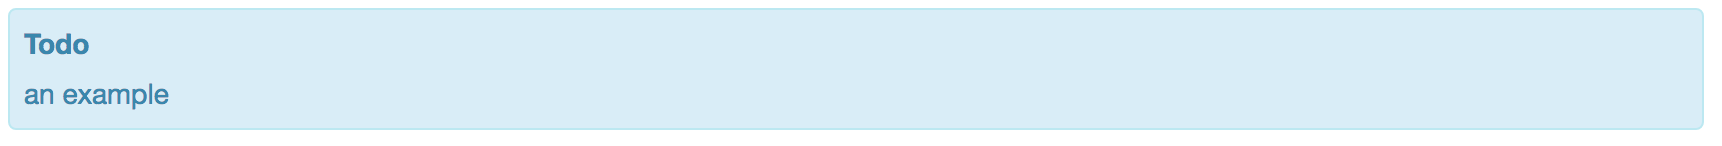
\includegraphics[width=\columnwidth]{../../images/todo.png}

\FILENAME

\section{Markdown}\label{markdown}

The content form this section originates from see:
\url{https://en.wikipedia.org/wiki/Markdown}.

Markdown is a simple markup language, however there is no precise
standard defined for it and implementations may have features not
supported by other implementations. Nevertheless, it provieds as imple
and easy way to quicly develop clean looking documents.

There are severla tools that make markdown attractive allowing to
write the text in one window while at the same time seeing the
rendered out put in another.

This includes

\begin{description}

\item[Macdown] An editor for mardown targeted on OSX

\end{description}

To convert the markdown to other formats with \verb|pandoc|

\begin{verbatim}
# Heading

## Sub-heading

### Another deeper heading
 
Paragraphs are separated
by a blank line.

Two spaces at the end of a line leave a  
line break.

Text attributes _italic_, *italic*, __bold__, **bold**, `monospace`.

Horizontal rule:

---

Bullet list:

  * apples
  * oranges
  * pears

Numbered list:

  1. apples
  2. oranges
  3. pears

A [link](http://example.com).

\end{verbatim}

\subsection{Tools}

\begin{description}
\item [Dilinger] \URL{https://dillinger.io/}. A HTML5 based cloud
  enabled editor. It allows to download the created Markdown.
\item[Macdown] \URL{https://macdown.uranusjr.com/} ``MacDown is an
  open source Markdown editor for macOS''
\end{description}
\FILENAME

\section{Communicating Research in Other Ways}\label{communicating-research}

Naturally, writing papers is not the only way to communicate your
research with others. We find that today we see additional pathways
for cumminication includine blogs, twitter, facebook, e-mail, Web
pages, and electronic notebooks. Let us refisit some of them and
identify when they are helpful.

\subsection{Blogs}\label{blogs}

\begin{description}
\item[blog:]
noun, a regularly updated website or web page, typically one run by an
individual or small group, that is written in an informal or
conversational style.
\end{description}

Advantages:

\begin{itemize}
\tightlist
\item
  encourages spontaneous posts
\item
  encourages small short contributions
\item
  chronologically ordered
\item
  standard software exists to set up blogs
\item
  online services exists to set up blogs
\end{itemize}

Disadvantages:

\begin{itemize}
\tightlist
\item
  structuring data is difficult (some blog software support it)
\item
  not suitable for formal development of a paper
\item
  often lack of sophisticated track change features
\item
  no collaborative editing features
\end{itemize}

\subsection{Sphinx}\label{sphinx}

Sphinx (\url{http://www.sphinx-doc.org/}) is a tool that to create
integrated documentation from a markup language whlie.

Advantages:

\begin{itemize}
\tightlist
\item
  output formats: html, LaTeX, PDF, ePub
\item
  integrates well with directory structure
\item
  powerful markup language (reStructuredText)
\item
  can be hosted on github via github pages
\item
  can integare other renderers such as Markdown
\item
  automatic table of content, tebale of index
\item
  code documentation integration
\item
  search
\item
  written in python and using bash, so extensions and custom automation
  are possible
\end{itemize}

Disadvantage:

\begin{itemize}
\tightlist
\item
  requires compile step
\item
  When using markdown github can render individual page
\end{itemize}

Others:

\begin{itemize}
\tightlist
\item
  Read the Docs (\url{https://readthedocs.org/})
\item
  Doxygen (\url{http://www.stack.nl/~dimitri/doxygen/})
\item
  MkDocs (\url{http://www.mkdocs.org/})
\end{itemize}

\subsection{Notebooks}\label{notebooks}

\subsubsection{Jupyter}\label{jupyter}

The Jupyter Notebook (\url{http://jupyter.org/}) is an open-source web
application allowing users to create and share documents that contain
live code, equations, visualizations and explanatory text. Use cases
include data cleaning and transformation, numerical simulation,
statistical modeling, machine learning.

Advantages:

\begin{itemize}
\tightlist
\item
  Integrates with python
\item
  Recently other programming languages have been integrated
\item
  Allows experimenting with settings
\item
  Allows a form of literate programming while mixing documentation with
  code
\item
  automatically renders on github
\item
  comes with web service that allows hosting
\end{itemize}

Disadvantage:

\begin{itemize}
\tightlist
\item
  mostly encourages short documents
\item
  mark up language is limited
\item
  editing in ASCII is complex and Web editing is prefered
\end{itemize}

\subsubsection{Apache Zeppilin}\label{apache-zeppilin}

A Web-based notebook that enables data-driven, interactive data
analytics and collaborative documents with SQL, Scala and hadoop. It
integrates a web-based notebook with data ingestion, data exploration,
visualization, sharing and collaboration features to Hadoop and Spark.

Advantages:

\begin{itemize}
\tightlist
\item
  integration to various framework
\item
  Web framework
\item
  integration with spark, hadoop
\end{itemize}

Disadvantages:

\begin{itemize}
\tightlist
\item
  larger framework
\item
  must leverages existing deployments of spak, hadoop
\end{itemize}


\begin{comment}
\subsection{References}\label{references}

Collaboratories:

\begin{itemize}
\tightlist
\item
  Myers JD, TC Allison, SJ Bittner, BT Didier, M Frenklach, WH Green, YL
  Ho, J Hewson, WS Koegler, CS Lansing, D Leahy, M Lee, R McCoy, M
  Minkoff, S Nijsure, G von Laszewski, D Montoya, L Oluwole, CM
  Pancerella, R Pinzon, W Pitz, LA Rahn, B Ruscic, KL Schuchardt, EG
  Stephan, A Wagner, TL Windus, and C Yang. 2005. ``A Collaborative
  Informatics Infrastructure for Multi-scale Science.'' Cluster
  Computing 8(4):243-253.
\item
  Metadata in the Collaboratory for Multi-Scale Chemical Science Carmen
  Pancerella, John Hewson, Wendy Koegler, David Leahy, Michael Lee,
  Larry Rahn, Christine Yang, James D. Myers, Brett Didier, Renata
  McCoy, Karen Schuchardt, Eric Stephan, Theresa Windus, Kaizar Amin,
  Sandra Bittner, Carina Lansing, Michael Minkoff, Sandeep Nijsure,
  Gregor von Laszewski, Reinhardt Pinzon, Branko Ruscic, Al Wagner,
  Baoshan Wang, William Pitz, Yen-Ling Ho, David Montoya, Lili Xu,
  Thomas C. Allison, William H. Green, Jr., Michael Frenklach
  \url{http://dcpapers.dublincore.org/pubs/article/view/740/736}
\end{itemize}
\end{comment}



%\chapter{Run Docker Locally on your Machine}\label{S:docker-local}

\FILENAME

\section{Installing Docker Community Edition}\label{installing-docker-community-edition}

To install docker on your computer, please visit the page:

\URL{https://www.docker.com/community-edition}{Docker Community Edition}

Here you will find a variety of packages, one of which will hopefully
suitable for your OS. The supported operating systems currently include:

\begin{itemize}
\item  OSX, Windows, Centos, Debian, Fedora, Ubuntu, AWS, Azure
\end{itemize}

Please chose the one most suitable for you.

\subsection{Instalation for OSX}\label{instalation-for-osx}

The docker community edition for OSX can be found at the following link

\href{https://store.docker.com/editions/community/docker-ce-desktop-mac?tab=description}{Information for OSX}

We recommend that at this time you get the version {\em Docker CE for MAC (stable)}

\URL{https://download.docker.com/mac/stable/Docker.dmg}

CLicking on the link will download a dmg file to your machine, that
you than will need to install by double clicking and allowing access
to the dmg file. Upon instalation a \texttt{whale} in the top status
bar shows that Docker is running, and you can acess it via a terminal.

\begin{figure}[htb]
\centering

\includegraphics[width=0.5\textwidth]{whale-in-menu-bar.png}
\caption{Docker integrated in the menu bar on OSX}
\end{figure}

\section{Testing if the install works}\label{testing-if-the-install-works}

To test if it works execute the following commands in a terminal:

\begin{verbatim}
docker version
\end{verbatim}

You should see an output similar to

\begin{verbatim}
docker version

Client:
  Version:      17.03.1-ce
  API version:  1.27
  Go version:   go1.7.5
  Git commit:   c6d412e
  Built:        Tue Mar 28 00:40:02 2017
  OS/Arch:      darwin/amd64

Server:
  Version:      17.03.1-ce
  API version:  1.27 (minimum version 1.12)
  Go version:   go1.7.5
  Git commit:   c6d412e
  Built:        Fri Mar 24 00:00:50 2017
  OS/Arch:      linux/amd64
  Experimental: true
\end{verbatim}

To see if you can run a container use

\begin{verbatim}
docker run hello-world
\end{verbatim}

Once executed you should see an outout similar to

\begin{verbatim}
Unable to find image 'hello-world:latest' locally
latest: Pulling from library/hello-world
78445dd45222: Pull complete 
Digest: sha256:c5515758d4c5e1e838e9cd307f6c6a .....
Status: Downloaded newer image for hello-world:latest

Hello from Docker!
This message shows that your installation appears to 
be working correctly.

To generate this message, Docker took the following steps:
1. The Docker client contacted the Docker daemon.
2. The Docker daemon pulled the "hello-world" image 
   from the Docker Hub.
3. The Docker daemon created a new container from that 
   image which runs the executable that produces the 
   output you are currently reading.
4. The Docker daemon streamed that output to the Docker 
   client, which sent it to your terminal.

To try something more ambitious, you can run an Ubuntu container 
with:

$ docker run -it ubuntu bash

Share images, automate workflows, and more with a free Docker ID:
https://cloud.docker.com/

For more examples and ideas, visit:
https://docs.docker.com/engine/userguide/
\end{verbatim}

%\chapter{Running Docker on FutureSystems}\label{S:docker-fg}

\FILENAME

\section{Overview}\label{overview}

This documentation introduces how to run Docker container on
FutureSystems. Currently we have deployed Docker swarm on Echo.

\section{Getting Access}\label{getting-access}

You will need an account on FutureSystems. To verify, try to see if you
can log into india.futuresystems.org. You need to be a member of a valid
FutureSystems project, and had submitted an ssh public key via the
FutureSystems portal.

If your access to the india host has been verified, try to login to the
docker swarm head node with the same username and key:

\textbf{NOTE: If you have access to india but not the docker swarm
system, your project may not have been authorized to access the docker
swarm cluster. Send a ticket to FutureSystems ticket system to request
this.}

Once logged in to the docker swarm head node, try to run:

to verify `docker run' works.

\section{Creating a service and deploy to the swarm
cluster}\label{creating-a-service-and-deploy-to-the-swarm-cluster}

While `docker run' can start a container and you may even attach to its
console, the recommended way to use a docker swarm cluster is to create
a service and have it run on the swarm cluster. The service will be
scheduled to one or many number of the nodes of the swarm cluster, based
on the configuration. It's also easy to scale up the service when more
swarm nodes are available. Docker swarm really makes it easier for
service/application developers to focus on the functionality development
but not worrying about how and where to bind the service to some
resources/server. The deployment, access, and scaling up/down when
necessary, are all managed transparently. Thus achieving the new
paradigm of `serverless computing'.

As an example, the following command creates a service and deploy it to
the swarm cluster:

\begin{quote}
docker service create --name notebook\_test -p 9001:8888
jupyter/datascience-notebook start-notebook.sh
--NotebookApp.password=NOTEBOOK\_PASS
\end{quote}

It pulls a published image from docker cloud, starts a container and
runs a script to start the service inside the container with necessary
parameters. The option ``-p 9001:8888'' maps the service port inside the
container (8888) to an external port of the cluster node (9001) so the
service could be accessed from the Internet. In this example, you can
then visit the URL:

\begin{quote}
\url{http://149.165.150.76:9001}
\end{quote}

to access the Jupyter notebook. Using the specified password when you
create the service to login.

Please note the service will be dynamically deployed to a container
instance, which would be allocated to a swarm node based on the
allocation policy. Docker makes this process transparent to the user and
even created mesh routing so you can access the service using the IP
address of the management head node of the swarm cluster, no matter
which actual physical node the service was deployed to.

This also implies that the external port number used has to be free at
the time when the service was created.

Some useful related commands:


\begin{verbatim}
docker service ls
\end{verbatim}

lists the currently running services.

\begin{verbatim}
docker service ps notebook_test
\end{verbatim}

lists the detailed info of the container where the service is running.

\begin{verbatim}
docker node ps NODE
\end{verbatim}

lists all the running containers of a node.

\begin{verbatim}
docker node ls
\end{verbatim}

lists all the nodes in the swarm cluster.

To stop the service and the container:

\begin{verbatim}
docker service rm noteboot_test
\end{verbatim}


\subsection{Create your own service}\label{create-your-own-service}

You can create your own service and run it. To do so, start from a base
image, e.g., a ubuntu image from the docker cloud. Then you could:

\begin{itemize}

\item Run a container from the image and attach to its console to develop
the service, and create a new image from the changed instance using
command `docker commit'.

\item Create a dockerfile, which has the step by step building process of
the service, and then build an image from it.

\end{itemize}

In reality, the first approach is probably useful when you are in the
phase of develop and debug your application/service. Once you have the
step by step instructions developped the latter approach is the
recommended way.

Publish the image to the docker cloud by following this documentation:

\begin{quote}
\url{https://docs.docker.com/docker-cloud/builds/push-images/}
\end{quote}

Please make sure no sensitive information is included in the image to
be published. Alternatively you could publish the image internally to
the swarm cluster.

\paragraph{Publish an image privately within the swarm cluster}
\label{publish-an-image-privately-within-the-swarm-cluster}

\TODO{Fugang: create image for distribution}

Once the image is published and available to the swarm cluster, you
could start a new service from the image similar to the Jupyter Notebook
example.


%\part{Preface}

\markdownInput{iu.md} 
 

%\part{Syllabus}

\chapter{Syllabus E516}

We present the syllabus for the E516 course tought at Indiana University that 
uses in part the material presented in this document. The information includes the section or chapter number, the name of the chapter or section, and the timeframe  when it is recommended to work through the material and the page number where to find the material in this document. Please note that we will update the document throughout the semester thus, pagenumbers will change. A specific date of publication whne the last update occured is 

\today~\currenttime 


\section{Communication Track}

\WHERE{c:doc}{(Month 1)}

\WHERE{S:plagiarism}{(Month 1)}

\WHERE{S:writing}{(Month 1)}

\WHERE{C:latex}{(Month 1)}

\WHERE{C:bibtex}{(Month 1)}

\WHERE{C:emacs}{(Optional, highly recommended)}

\WHERE{S:markdown}{(Month 1)}


\section{Theory Track}



\section{Programming Track}

\section{Cluster Track}

\chapter{Syllabus E616}

We present the syllabus for the E516 course tought at Indiana University that 
uses in part the material presented in this document. The information includes the section or chapter number, the name of the chapter or section, and the timeframe  when it is recommended to work through the material and the page number where to find the material in this document. Please note that we will update the document throughout the semester thus, pagenumbers will change. A specific date of publication whne the last update occured is

\today~\currenttime 

\section{Communication Track}

\WHERE{c:doc}{(Month 1)}

\WHERE{S:plagiarism}{(Week 1)}

\WHERE{S:writing}{(Week 1)}

\WHERE{C:latex}{(Week 2)}

\WHERE{C:bibtex}{(Week 2)}

\WHERE{C:emacs}{(Week 1, Optional, highly recommended)}

\WHERE{S:markdown}{(Week1)}


\section{Theory Track}


\section{Programming Track}

\subsection{Development Environment}

\WHERE{C:linux-shell}{Week 2}

\WHERE{C:github}{Week 3}

\WHERE{S:virtual-box}{Week 3}

\subsection{Python}

\WHERE{P:python}{Week 3 - 4}

\WHERE{c:numpy}{}

\WHERE{c:scipy}{} 

\WHERE{c:opencv}{}

\WHERE{c:secchi-disk}{}

\section{Cluster Track}

\WHERE{c:pi-cluster-form-factor}{(Month 1)}

%\section{I524 Lectures}\label{i524-lectures}



\begin{description}
\item[This page is under construction, but most lectures are]
already available. All tracks will change considerably. If you want to
work ahead, start with the theory track.
\end{description}

\begin{description}
\item[At the end of the page, you find a link to unreleased]
lectures.
\end{description}

Based on our experience with residential and online classes we will for
the first time not require that you have to do the class videos at a
particular time once they are released. This, however, has the danger
that you are not watching them at all and you cheat yourself as you do
not allow yourself the educational lessons that this class offers to
you. It also requires you to assemble your own schedule for watching the
videos that will have to be managed through Github as part of a
README.md file in your git repository. You will need to do the
technology track, the communications track, as well as the theory track.

\begin{description}

\item[Theory Track:]
Some lectures have been designed to introduce you to a number of
technologies. These lectures are of more theoretical nature and do not
require much hands on activities. Thus you can start them any time.

\item[Collaboration Track:]
These lectures provide the tools for you to collaborate with your peers
and with instructors.

\item[Systems Track:]
These lectures cover topics that are fundamental to executing your
project.

\item[Technology Track:]
These are lectures with strong technology content and introduce you to
using a selected number of technologies as part of the class. It is
expected that you will use them as part of the project. Instead of
slowing you down with graded homework we expect that you learn these
technologies and reuse them as part of the project. It would be a big
mistake to start the project 2 weeks before the semester ends, you will
not succeed. You must start your project in the first month of the
course. Progress is reported on a monthly basis while the report is
updated and snapshot every month. We will monitor your progress and
include them into the discussion grade. For residential students there
should be no reason why you can not provide a monthly update. For online
students, a valid update would be: ``I changed my company and could not
work on the project due to moving''. This will give you some points if
submitted in time. However, if you submit nothing, we will not issue any
points.

\end{description}

\subsection{Lectures - Theory Track}\label{lectures---theory-track}


\subsubsection{Overview}

\slides{i524}{Pages ??}{Overview}{https://drive.google.com/file/d/0Bx_sUfI4VkKSaHlDWkZkeGh4LVE/view?usp=sharing}

\video{i524}{11:29}{Part 1}{https://www.youtube.com/watch?v=Z2M5NsTsj2Y}

\video{i524}{04:10}{Part 2, Video }{https://www.youtube.com/watch?v=5VXhF_Z7Vdk}

\video{i524}{12:41}{Part 3, Video }{https://www.youtube.com/watch?v=DDXqLZcavas}

\subsubsection{Web Page}

,Course Web Page, Web Page \url{https://cloudmesh.github.io/classes/index.html},

\video{i524}{11:25}{Part 1,Video }{https://www.youtube.com/watch?v=uE45GE1Ceok}

\video{i524}{17:31}{Part 2,Video }{https://www.youtube.com/watch?v=Tkhu96TreMk}

\subsection{Technology List}

Web Page \url{https://cloudmesh.github.io/classes/i524/technologies.html}, 

\video{i524}{ 40:08}{TechList.1 Homework, Video }{https://www.youtube.com/watch?v=roi7vezNmfo}

\subsubsection{Introduction}

Course Introduction,Slides \url{https://drive.google.com/file/d/0Bx_sUfI4VkKSMHBUblVUMWg4Y00/view?usp=sharing}

\video{i524}{0:13:59}{Introduction,Video }{https://www.youtube.com/watch?v=VWK7QdThOPQ}

\video{i524}{0:15:28}{Real World Big Data,Video }{https://www.youtube.com/watch?v=hjrFaXMU1dg&list=PLLO4AVszo1SNIGlqjEBaQjLvc3lgpeI3M&index=2}

\video{i524}{0:10:57}{Basic Trends and Jobs,Video }{https://www.youtube.com/watch?v=u5Y0aKbzync&index=3&list=PLLO4AVszo1SNIGlqjEBaQjLvc3lgpeI3M}

Acess Patterns, Data Access Patterns and Introduction to using HPC-ABDS,Slides \url{https://iu.box.com/s/o5rqlsop0jv98lqdon3h9qszk3soq31g}

\video{i524}{0:27:45}{A. Introduction to HPC-ABDS Software and Access Patterns,Video }{https://www.youtube.com/watch?v=6Kj9E38lUzU}

-  Resource 1  \url{http://grids.ucs.indiana.edu/ptliupages/publications/HPC-ABDSDescribedv2.pdf}

\video{i524}{0:18:38}{B. Science Examples (Data Access Patterns),Video }{https://www.youtube.com/watch?v=hYJ4_1A4kEU}

-  Resource 2 \url{http://hpc-abds.org/kaleidoscope/}

\video{i524}{0:11:26}{C. Remaining General Access Patterns,Video }{https://www.youtube.com/watch?v=hsEDKM7Zur4}

\video{i524}{0:14:32}{D. Summary of HPC-ABDS Layers 1 - 6,Video }{https://www.youtube.com/watch?v=zVPKiGV0fk0}

\video{i524}{0:30:52}{E. Summary of HPC-ABDS Layers 7 - 13,Video }{https://youtu.be/6Kj9E38lUzU}

\video{i524}{0:28:02}{F. Summary of HPC-ABDS Layers 14 - 17,Video }{https://www.youtube.com/watch?v=13EQZ-6z91k}

\video{i524}{0:20:20}{Final Part Summary of Stack,Video }{https://www.youtube.com/watch?v=0kj-NEl8VF4}

\subsubsection{Application Structure}

Big Data Application Structure,Slides \url{https://iu.box.com/s/zl71trvqfw6vv4wnc8xr6gf1qpc9a2dr}

\video{i524}{0:23:25}{NIST Big Data Sub Groups,Video }{https://www.youtube.com/watch?v=12-BlQhnCxc}

\video{i524}{0:23:51}{Big Data Patterns - Sources of Parallelism,Video }{https://www.youtube.com/watch?v=tZfFQw5M8cU}

\video{i524}{0:18:26}{First and Second Set of Features,Video }{https://www.youtube.com/watch?v=PgUGXql34DM}

\video{i524}{0:18:38}{Machine Learning Aspect of Second Feature Set and the Third Set,Video }{https://www.youtube.com/watch?v=mNmmW5ZBjgs}

\subsubsection{Application Aspects}

Aspects of Big Data Applications,Slides \url{https://iu.box.com/s/atgkxucop1lzftkunf8al2fe74x65na6}

\video{i524}{0:16:50}{Other sources of use cases and Classical Databases/SQL Solutions,Video }{https://youtu.be/dZRtHaf2MyA}

\video{i524}{0:18:49}{SQL Solutions -  Machine Learning Example -  and MapReduce,Video }{https://www.youtube.com/watch?v=PZDiJNS234A}

\video{i524}{0:20:26}{Clouds vs HPC -  Data Intensive vs. Simulation Problems,Video }{https://www.youtube.com/watch?v=gazESBGLlY8}

\subsubsection{Applications}

Big Data Applications and Generalizing their Structure,Slides \url{https://iu.box.com/s/01dndtucmynekgehur00vktfgcppgc1r}

\video{i524}{0:25:20}{NIST UseCases and Image Based Applications Examples I,Video }{https://www.youtube.com/watch?v=tRoAx444A6U}

\video{i524}{0:15:23}{Image Based Applications II,Video }{https://www.youtube.com/watch?v=FDtnWGwotjA}

\video{i524}{0:25:25}{Internet of Things Based Applications,Video }{https://www.youtube.com/watch?v=cOuCSveoVYY}

\video{i524}{0:22:44}{Big Data Patterns - the Ogres and their Facets I,Video }{https://www.youtube.com/watch?v=CvCfRP7J6dU}

\video{i524}{0:15:09}{Facets of the Big Data Ogres II,Video }{https://www.youtube.com/watch?v=fGyUPApnwHw}

\subsubsection{Other}

\video{i524}{0:24:00}{More of Software Stack,Video }{https://www.youtube.com/watch?v=apDXH_eVnEc}

\subsection{Lectures - Collaboration Track}\label{lectures---collaboration-track}


\subsubsection{Organization}
 Lessons vs Lectures, Web Page \url{../lesson/org/index.html},
\subsubsection{Piazza}
 Information about Piazza, PDF \url{https://piazza.com/pdfs/piazza_product_introduction.pdf},
\subsubsection{Web Page}
 Contributing to the Web Page, Web Page \url{../lesson/contrib/contributing.html},


\subsubsection{Github}
 

Overview and Introduction, Web page \url{../lesson/prg/github.html#video-lectures-on-github}

Install Instructions, Web page  \url{https://www.atlassian.com/git/tutorials/install-git}
 
\video{i524}{2:47}{config, Video }{https://www.youtube.com/watch?v=ZChtKFLiaNw}

\video{i524}{1:41}{fork, Video }{https://www.youtube.com/watch?v=5oJHRbqEofs}

\video{i524}{3:11}{checkout, Video }{https://www.youtube.com/watch?v=HwrPhOp6-aM}

\video{i524}{4:26}{pull, Video }{https://www.youtube.com/watch?v=d5wpJ5VimSU}

\video{i524}{2:25}{branch, Video }{https://www.youtube.com/watch?v=H5GJfcp3p4Q}

\video{i524}{4:50}{merge, Video }{https://www.youtube.com/watch?v=yyLiplDQtf0}

\video{i524}{4:20}{rebase, Video }{https://www.youtube.com/watch?v=SxzjZtJwOgo}

\video{i524}{3:47}{GUI, Video }{https://www.youtube.com/watch?v=BMYOs5jflGE}

\video{i524}{1:25}{Windows - unsupported, Video }{https://www.youtube.com/watch?v=YBbkvCrfDSo}


\subsubsection{Paper}


\video{i524}{ 34:24}{How to write a paper by Simon Peyton Jones, Video }{https://www.youtube.com/watch?v=g3dkRsTqdDA}

\video{i524}{}{LaTeX - Overview of LaTeX Resources, Web Page }{../lesson/doc/latex.html}

\video{i524}{ 8:49}{(optional) ShareLaTeX, Video }{https://youtu.be/PfhSOjuQk8Y}

\video{i524}{14:41}{jabref, Video }{https://youtu.be/cMtYOHCHZ3k}

bibtex, Web Page \url{../lesson/doc/bibtex.html},

Report Format, Web Page \url{../lesson/doc/report.html} 

Git \url{https://github.com/cloudmesh/classes/tree/master/docs/source/format/report}

PDF \url{https://github.com/cloudmesh/classes/tree/master/docs/source/format/report},

Advice based on paper 1 submissions,Web Page \url{paper-advice},,Mar 30



\subsubsection{RST}
, (Draft) Restructured Text, Web Page \url{../lesson/doc/rst.html},


\subsection{Lectures - Systems}\label{lectures---systems}

Ubuntu, Development OS for the class, Web page \url{../lesson/linux/ubuntu}

Virtualbox, Virtualbox for class, Web page \url{../lesson/linux/virtualbox}

  , Instalation of ubuntu in virtualbox, Video \url{https://youtu.be/NWibDntN2M4}

  , Instalation of guest additions in virtualbox, Video \url{https://youtu.be/wdCoiNdn2jA}

Shell, Linux Shell, Video \url{https://www.youtube.com/watch?v=LeTlm_ck2GI} | Web Page \url{../lesson/linux/linux}

Python, Introduction to Python, Web page \url{../lesson/prg/python_intro}

      , Python for Big Data, Web Page \url{../lesson/prg/python_big_data}

      , Python CMD, Web Page \url{../lesson/prg/python_cmd}

      , Python CMD5, Web Page \url{../lesson/prg/python_cmd5},,Mar 30

      , Cloudmesh.rest, Web Page \url{../lesson/prg/rest},,Mar 31     

      , (Optional) Python pyenv, Web Page \url{../lesson/prg/pyenv},,Feb 24

      , (Draft - Advanced) Python Fingerprint example, Web page \url{../lesson/prg/python_lesson1}

\video{i524}{Minutes ????}{PyCharm, Video }{https://www.youtube.com/watch?v=X8ZpbZweJcw}

Refcards, Reference cards, Web Page \url{../lesson/linux/refcards}

Emacs, (Optional) Useful emacs commands, Web Page \url{../lesson/doc/emacs}

\video{i524}{Minutes ???}{Cloudmesh Client,Installation of Cloudmesh Client}{https://www.youtube.com/watch?v=R50IQYhr-vg} 

| Web Page \url{../lesson/cloud/cloudmesh-installation},,Feb 14

\video{i524}{Minutes ???}{Setting up a cluster and Hadoop, Pig, and Spark with Cloudmesh,    Video }{https://www.youtube.com/watch?v=KOV8PqvX-GQ} 

Web Page \url{../lesson/devops/hadoop},,Mar 20

Use only one public IP address, Web Page \url{../lesson/cloud/cm-cluster-with-one-ip},,Apr 11

\video{i524}{Minutes ???}{Ansible, Starting Point, Video }{https://www.youtube.com/watch?v=no52OmHg1ek} 

Web Page \url{../lesson/devops/ansible/ansible-I},,Feb 14

\video{i524}{Minutes ???}{Roles and Others, Video       }{https://www.youtube.com/watch?v=eN52x5XxJAE} 

Web Page \url{../lesson/devops/ansible/ansible-II},,Feb 14

Ansible Galaxy, Web Page \url{../lesson/devops/ansible/ansible-III},, Feb 14


\subsection{Lectures -Tech}

Unit 4, FutureSystems Openstack, , 

\video{i524}{ 0:12:00}{Unit 4.A, Introduction and Overview, Video }{https://mix.office.com/watch/u7uovy9i06jo}

Unit.Linux, Linux Basics - Overview - Shell Scripting -  Editors (Emacs - vi - nano - pico - PyCharm), ,

Unit.Linix.2, Python - Package Managers - Advanced SSH - Modules, ,

Unit.VM.1, shared resources - install image -  start vm -  loginto vm using your local key from the VB using command line tools and not web client, ,

Unit.Cloud.1, Introduction to Cloud Computing, , 

Unit.Cloud.2, IaaS: OpenStack, ,

Unit.Cloud.2.1, IaaS: Nova, Web Page \url{../lesson/iaas/openstack},

X.Unit.Cloud.2.2, IaaS: Nova, H2 \url{http://cloudmesh.github.io/introduction_to_cloud_computing/class/lesson/iaas/openstack.html#exercises} ,

X.Unit.Cloud.2.3, IaaS: Nova, H2-2: Horizon \url{http://cloudmesh.github.io/introduction_to_cloud_computing/class/lesson/iaas/openstack_horizon.html#exercises},

Unit.Cloud.3, IaaS: Azure, Web page \url{../lesson/iaas/azure},  

Unit.Cloud.4, Hybrid Clouds, Cloudmesh \url{https://mix.office.com/watch/1c7rd1l9i4c8o},

Unit.DevOps.1.3, Ansible, Web page \url{../lesson/devops/ansible},

Unit.Devops.2.1, SaltStack, Web page \url{../lesson/devops/saltstack}, 

X.Unit.DevOps.2.2, SaltSalt, Web Page page \url{http://cloudmesh.github.io/introduction_to_cloud_computing/class/lesson/devops/saltstack.html#ref-class-lesson-devops-saltstack-exercises}, 

Unit.DevOps.2.1, Puppet, Web page \url{../lesson/devops/puppet}, 

\video{i524}{ 0:35:00}{Unit.DevOps.2.2, Chef, Chef }{https://mix.office.com/watch/1g90jbv8llv0j}

Unit.DevOps.2.3, Chef, Web page \url{../lesson/devops/chef}, 

\video{i524}{ 0:20:00}{Unit.DevOps.4.1, OpenStack Heat, Video }{https://mix.office.com/watch/1ry7jrkuvkfwh}

Unit.DevOps.4.2, OpenSrack Heat, Web page \url{../lesson/devops/openstack_heat}, 

X.Unit.Devops.4.3, H4-2: Heat, Web page \url{http://cloudmesh.github.io/introduction_to_cloud_computing/class/lesson/devops/openstack_heat.html#ref-class-lesson-devops-openstack-heat-exercises}, 

Unit.DevOps.5.1, Ubuntu Juju, Web page \url{..//lesson/devops/juju}, 

X.Unit.DevOps.5.2, Ubuntu Juju, H: Juju  \url{http://cloudmesh.github.io/introduction_to_cloud_computing/class/lesson/devops/juju.html#ref -class -lesson -devops -juju -exercises}, 

R.Hadoop.1, Hadoop, Web page \url{http://cloudmesh.github.io/introduction_to_cloud_computing/class/vc_sp15/hadoop_cluster_manual.html#ref-class-lesson-deploying-hadoop-cluster-manual}, 

X.Hadoop.2, Hadoop, ext H: Hadoop \url{http://cloudmesh.github.io/introduction_to_cloud_computing/class/vc_sp15/hadoop_cluster_manual.html#ref-class-lesson-deploying-hadoop-cluster-manuale-exercise}  , 

\video{i524}{   0:33:00}{Hadoop.3, Hadoop Word Count, Video }{https://mix.office.com/watch/1on4q8t1vcjfh}

F.Hadoop.4, Hadoop Word Count, Web page \url{http://cloudmesh.github.io/introduction_to_cloud_computing/class/lesson/cluster/wordcount.html#ref-class-lesson-hadoop-word-count}  , 

\video{i524}{  0:04:00}{Mongo.1, Mongo, Video  }{https://mix.office.com/watch/1rx90yz48fqpn}

Mongo.2, Mongo, Web page \url{../lesson/database/mongodb_cluster}, 

\video{i524}{   0:04:00   }{VirtualClusters.1, Introduction and Overview, Video }{https://mix.office.com/watch/eap9zdqfifgp}

\video{i524}{   0:04:00}{VirtualClusters.2, Dynamic Deployment of Arbitrary X Software on Virtual Cluster,  Video }{https://mix.office.com/watch/zukoz9wswe7z}

\video{i524}{   0:34:00}{VirtualCluster.3.1, Apache Hadoop YARN, Video }{https://mix.office.com/watch/1eopy3tfq6kim}

VirtualCluster.3.2, Apache Hadoop YARN, Web page \url{../lesson/tech/yarn},   

\video{i524}{   0:40:00}{VirtualCluster.3.3, Apache Zookeeper, Apache ZooKeeper }{https://mix.office.com/watch/1ptxm2uj2s7y3}

VirtualCluster.3.4, Apache Zookeeper, Web page \url{../lesson/tech/zookeeper}, 

F.VirtualCluster.4, Open MPI Virtual Cluster,  Web page \url{../lesson/tech/openmpi},

Cluster.1, HPC Queuing System, Web page \url{../lesson/tech/hpc},

Docker.1, Docker Basics, Web page \url{../lesson/tech/docker} ,

VM.1, VM Software - Vagrant, Web page \url{../lesson/tech/vagrant}, 

X.Hadoop.x, Hadoop MRv2, Web page \url{http://cloudmesh.github.io/introduction_to_cloud_computing/class/lesson/cluster/hadoop2.html#ref-class-lesson-hadoop2} ,



\subsection{Unreleased Lectures}\label{unreleased-lectures}

A list of unreleased lectures that we are currently working on is
available here: ref-unreleased



%%----------------------------------------------------------------------------------------
%	PART
%----------------------------------------------------------------------------------------

\part{Documenting Scientific Research}

\FILENAME

%----------------------------------------------------------------------------------------
%	CHAPTER 1
%----------------------------------------------------------------------------------------

\chapterimage{writing.png} % Chapter heading image

\chapter{Documenting Scientific Research}

\FILENAME

\section{Plagiarism}\label{S:plagiarism}

We start with the review of a most important topic.

\subsection{Plagiarism Definition}

In academic life it is important to understand and avoid plagiarism.
The dictionary defines plagiarism as follows \url{dictionary.com}:

% \textipa{['pl\=aj@""riz@m]}

\begin{description}
\item[pla·gia·rism] ``the practice of taking someone else's work or ideas and passing them
off as one's own.''
\end{description}



\subsection{Plagiarism Policies}
Organizations and universities will have policies in place do address
plagiarism. An example is provided for Indiana University
\cite{www-iu-plagiarism}. We quote:

\begin{quotation}
``Honesty requires that any ideas or materials taken from
another source for either written or oral use must be fully
acknowledged. Offering the work of someone else as one’s own is
plagiarism. The language or ideas thus taken from another may range
from isolated formulas, sentences, or paragraphs to entire articles
copied from books, periodicals, speeches, or the writings of other
students. The offering of materials assembled or collected by others
in the form of projects or collections without acknowledgment also is
considered plagiarism. Any student who fails to give credit for ideas
or materials taken from another source is guilty of plagiarism. 

(Faculty Council, May 2, 1961; University Faculty Council, March 11,
1975; Board of Trustees, July 11, 1975)''
\end{quotation}

Faculty members at Universitys are also bound by policies that mandate
reporting. At Indiana University the following policy applies (for a
complete policy see the Web page):

\begin{quotation}
``Should
the faculty member detect signs of plagiarism or cheating, it is his
or her most serious obligation to investigate these thoroughly, to
take appropriate action with respect to the grades of students, and
\textit{in any event} to report the matter to the Dean for Student Services [or
equivalent administrator]. The necessity to report every case of
cheating, whether or not further action is desirable, arises
particularly because of the possibility that this is not the student’s
first offense, or that other offenses may follow it. Equity also
demands that a uniform reporting practice be enforced; otherwise, some
students will be penalized while others guilty of the same actions
will go free.

(Faculty Council, May 2, 1961)''
\end{quotation}

Naturally if a student has any questions about understanding
plagiarism the University can provide assistance. If a student is in
doubt and asks for help this is not considered at that time
plagiarism. 

As you can see from the previous policies, the faculty do not have any
choice but reporting real cases of plagiarism to the university
administration.  Thus you must not hold them personally responsible as
this is part of the tasks they are required to do if they like it or
not. Instead, it is {\bf the responsibility of the authors of the
  document} to assure no plagiarism occurs. If you are a student of a
class that writes a paper or project report this naturally also all
applies to you. In addition, if you work in a team you need to assure
the entire team addresses plagiarism appropriately.

In practice this means that the teachers of a course expect yo know
plagiarism and you need to be informed about it. This is typically
done in other courses. However, as it is often overlooked by the
student we are pointing it out here so we can make sure you contribute
to courses that require you to write papers and reports. This also
means you can not claim you did not know what plagiarism is. You are
required to know what it is, know how to detect it and know how to
avoid it. The resources provided next will give you the necessary
tools and background.

\subsection{Plagiarism Resources}

The \href{http://education.indiana.edu/}{School of Education at Indiana
University} has a significant set of resources to get educated about
plagiarism. These resources are intended to ``preparing educators,
advancing knowledge, and improving education'' \cite{}
\url{https://www.indiana.edu/~istd/patterns.html}

The content here is copied from the Web Page

  \URL{https://www.indiana.edu/~istd/patterns.html}

As such we have not included quotes but refer to their Web page for the
original source which may also include updates. Naturally we do not want
to be accused of plagiarize in a chapter about plagiarism.  Thus assume
the content for the rest ov this chapter are copied from that Web page.

\subsection{Pattern}\label{pattern}

\begin{itemize}
\item
  \href{https://www.indiana.edu/~istd/definition.html}{IU Definition} of
  Plagiarism from Student Code of Conduct
\item
  \href{https://www.indiana.edu/~istd/overview.html}{Overview} How to
  give proper credit, steps.
\item
  \href{https://www.indiana.edu/~istd/cases.html}{Cases} of Plagiarism
  in the US, in the news, and elsewhere
\item
  \href{https://www.indiana.edu/~istd/examples.html}{Examples} Word for
  word, paraphrasing
\item
  \href{https://www.indiana.edu/~istd/practice.html}{Practice} with
  feedback on word-for-word and paraphrasing plagiarism
\item
  \href{https://www.indiana.edu/~istd/test.html}{Test} 10 questions on
  recognizing plagiarism
\item
  \href{https://www.indiana.edu/~istd/sitemap.html}{Tutorial Site Map}
  Expanded table of contents
\item
  \href{https://www.indiana.edu/~istd/resources.html}{Resources}
  Websites, books, dictionary links, references for learning more about
  plagiarism
\end{itemize}

\subsection{Tutorials}\label{S:ptutorial}

A number of tutorials are offerd by Indiana University \href{http://education.indiana.edu/graduate/programs/instructional-systems/index.html}{Instructional
  Systems Technology Department}
 Web pages ealing with plagiarism. Thes include:

\begin{itemize}
\item
  \href{https://www.indiana.edu/~academy/firstPrinciples/choice.html}{Plagiarsim
    Tutorial}
\item
  \href{https://www.indiana.edu/~tedfrick/plagiarism/}{Understanding
  Plagiarism}
\end{itemize}

\subsection{How to Recognize Plagiarism}

We are listing fifteen patterns of plagiarism that are defined on the Web
pages itedntified in Section~\ref{S:ptutorial}:

\begin{tabular}{p{4cm}p{3cm}p{8cm}}
Name & Plagiarism Type & Reason \\
\hline
  \href{patternCluelessQuote.html}{Clueless Quote} &  word-for-word & no
  quotes, no citation, no reference 
\\
  \href{patternCraftyCoverUp.html}{Crafty Cover-up} &  proper paraphrase
  but word-for-word  &  also present
\\
  \href{patternCunningCoverUp.html}{Cunning Cover-up} &  paraphrasing & no
  citation, no reference
\\
  \href{patternDeceptiveDupe.html}{Deceptive Dupe} &  word-for-word  &  no
  quotes, no citation, but has reference
\\
  \href{patternDisconnectedDupe.html}{Delinked Dupe} &  word-for-word  &  no
  reference, even though quotes and citation
\\
  \href{patternDeviousDupe.html}{Devious Dupe} &  correct quote but word-for-word  & 
  also present
\\
  \href{patternDippyDupe.html}{Dippy Dupe} &  word-for-word  &  quotes
  missing, even though full citation and reference
\\
  \href{patternDisguisedDupe.html}{Disguised Dupe} &  looks like proper
  para, but actually word-for-word  &  no quotes, no locator
\\
  \href{patternDoubleTrouble.html}{Double Trouble} & word-for-word  and
  paraphrasing  & although has reference
\\
  \href{patternLostLoser.html}{Linkless Loser} &  word-for-word  &  citation
  and reference lacking, although has quotes and locator
\\
  \href{patternLostLocator.html}{Lost Locator} &  word-for-word  &  missing
  locator, although has quotes, citation, and reference
\\
  \href{patternPointlessParaphrase.html}{Placeless Paraphrase} &  paraphrasing  & 
  no reference, although citation present
\\
  \href{patternSeveredCite.html}{Severed Cite} &  paraphrasing  &  reference
  but no citation
\\
  \href{patternShirkingCite.html}{Shirking Cite} &  word-for-word  &  lacks
  locator and reference, although quotes and citation present
\\
  \href{patternTripleD.html}{Triple D--Disguised Disconnected Dupe} & 
  word-for-word  & looks like proper para, but no quotes, no reference, no locator
\end{tabular}

In addition they do specify  three patterns of
non-plagiarism:

\begin{tabular}{p{2cm}p{4cm}p{8cm}}
Name & Type & Description \\
\hline
\\
  \href{patternCorrectQuote.html}{Correct Quote} &  non-plagiarizm & takes another's words
  verbatim and acknowledges with quotation marks, full in-text citation
  with locator, and reference
\\
  \href{patternProperParaphrase.html}{Proper Paraphrase} &  non-plagiarizm & summarizes
  another's words and acknowledges with in-text citation and reference
\\
  \href{patternMindlessParaphrase.html}{Parroted Paraphrase} &  non-plagiarizm & appears to
  be paraphrasing, and technically may not be plagiarism, but \ldots{}
  ???
\end{tabular}


\FILENAME

\section{Writing a Scientific Article or Conference Paper}
\index{Writing}

An important part of any scientific research is to document it. This is
often done through scientific conferences or journal articles. Hence it
is important to learn how to prepare and submit such papers. Most
conferences accept typically the papers in PDF format but require the
papers to be prepared on MSWord or in LaTeX. While working with many
students in the past we noticed however that those students using Word
often spend unnecessarily countless hours on trying to make there papers
beautiful while actually violating the template provided by the
conference. Furthermore, we noticed that the same students had issues
with bibliography management. Instead of Word helping the student it
provided the illusion to be easier than LaTeX but when adding up the
time spend on the paper we found that LaTeX actually saved time. This
has been especially true with the advent of collaborative editing
services such as sharelatex \cite{www-sharelatex} and overleaf
\cite{www-overleaf}. 

In this section we provide you with a professional template that is used
for either system based on the ACM standard that you can use to write
papers. Naturally this will be extremely useful if the quality of your
research is strong enough to be submitted to a conference. We structure
this section as follows. Although we do not recommend that you use
MSWord for your editing of a scientific paper, we have included a short
section about it and outline some of its pitfalls that initially you may
not think is problematic, but has proven to be an issue with students.
Next we will focus on introducing you to LaTeX and showcasing you the
advantages and disadvantages. We will dedicate an entire section on
bibliography management and teach you jhow to use jabref which clearly
has advantages for us.

Having a uniform report format not only helps the students but allow
allows the comparison of paper length and effort as part of teaching a
course. We have added an entire section to this chapter that discusses
how we can manage a \emph{Class Proceedings} form papers that are
contributed by teams in the class.

\subsection{Professional Paper Format}\label{professional-paper-format}

The report format we suggest here is based on the standard ACM
proccedings format. It is of very high quality and can be adapted for
your own activities. Moreover, it is possible to use most of teh text to
adapt to other formats in case the conference you intend to submit your
paper to has a different format. The ACM format is always a good start.

Important is that you do not need to change the template but you can
change some parameters in case you are not submitting the paper to a
conference but use it for class papers. Certainly you should not change
the spacing or the layout and instead focus on writing content. As for
bibliography management we recommend you use jabref which we will
introduce in Section \ref{??}.

We recommend that you carefully study the requirements for the report
format. We would nat want that your paper gets rejected by a journal,
conference or the class just because you try to modify the format or do
not follow the established publication guidlines.

The template we are providing is available from:

\URL{https://github.com/cloudmesh/classes/tree/master/docs/source/format/report}

Convenient compressed files are available at

\URL{https://github.com/cloudmesh/classes/tree/master/docs/source/format/report.tar.gz}
\URL{https://github.com/cloudmesh/classes/tree/master/docs/source/format/report.zip}

You will find in it a modified ACM proceedings templates for Word and
for LaTeX that has an identification box removed on the lower left hand
side of the first page. This is done for classes so that you have more
space to write. In case you must submit to a conference you can use the
original ACM template. This template can be found at

\subsection{Submission Requirements}\label{submission-requirements}

Although the initial requirement for some conferences or journals is the
document PDF, in many cases you must be prepared to provide the source
when submitting to the conference. This includes the submission of the
original images in an images foder. You may ba asked to package the
document into a folder with all of its sources and submit to the
conference for professional publication.

\subsection{Microsoft Word vs. \LaTeX}\label{microsoft-word}

Microsoft word will provide you with the initial impression that you
will safe lots of time writing in it while you see the layout of the
document. This will be initially true, but once you progress to the
more challenging parts and later pages such as image menagement and
bibliography management you will see some issues. Thes include that
figure placement in Word need sto be done just right in order for images
to be where they need. We have seen students spending hours with the
placement of figures in a paper but when they did additional changes the
images jumped around and were not at the place where teh students
expected them to be. So if you work with images, make sure you
understand how to place them. Also always use relative caption counters
so that if an image gets placed elsewhere the counter stays consistent.
So nefer use just the number, but a reference to the figure when referring
to it. Recently a new bibliography management system was added to Word.
However, however it is not well documented and the references are placed
in the system bibliography rather than a local managed bibliography.
This mah have severe consequences when working with many authors on a
paper. The same is true when using Endnote. We have heard in many
occasions that the combination of endnote and Word destroyed documents.
You certainly do not want that to happen the day before your deadline.
Also in classes we observed that those using LaTeX deliver better
structured and written papers as the focus is on text and not beautiful
layout.

For all these reasons we do not recommend that you use Word.

In LaTeX where we have an easier time with this as we can just ignore
all of these issues due to relative good image placement and excellent
support for academic reference management. Hence, it is in your best
interest to use LaTeX. The information we provide here will make it easy
for you to get started and write a paper in no time as it is just like
filling out a form.

\subsection{Working in a Team}\label{working-in-a-team}

Today research is done in potentially large research teams. This also
include the writing of a document. There are multiple ways this is done
these days and depends on the system you chose.

In MSWord you can use skydrive, while for LaTeX you can use sharelatex
and overleaf. However, in many cases the use of github is possible as
the same groups that develop the code are also familiar with github.
Thus we provide you here also with the introduction on how to write a
document in github while group members can contribute.

Here are the options:

\begin{description}

\item [LaTeX and git:] This option will likely safe you time as you can use
  jabref also for managing collaborative bibliographies and
\item [sharelatex:] an online tool to write latex documents
\item [overleaf:] an online tool to write latex documents
\item [MS onedrive:] It allows you to edit a word document in collaboration.
  We recommend that you use a local installed version of Word and do the
  editing with that, rather than using the online version. The online
  editor has some bugs. See also (untested):
  \url{http://www.paulkiddie.com/2009/07/jabref-exports-to-word-2007-xml/},
  \url{http://usefulcodes.blogspot.com/2015/01/using-jabref-to-import-bib-to-microsoft.html}
\item [Google Drive:] google drive could be used to collaborate on text that
  is than pasted into document. However it is just a starting point as
  it does not support typically the format required by the publisher.
  Hence at one point you need to swithc to one of the other systems.
\end{description}

\subsection{Timemanagement}\label{timemanagement}

Obviously writing a paper takes time and you need to car-fully make sure
you devote enough time to it. The important part is that the paper
should not be an after thought but should be the initial activity to
conduct and execute your research. Remember that

\begin{enumerate}

\item  It takes time to read the information
\item  It takes time understand the information
\item  It takes time to do the research

\end{enumerate}

For deadlines the following will get you in trouble:

\begin{enumerate}

\item
  \emph{There are still 10 weeks left till the deadline, so let me start
  in 4 week \ldots{}}. Procrastination is your worst enemy.
\item
  If you work in a team that has time management issues address them
  immediately
\item
  Do not underestimate the time it takes to prepare the final submission
  into the submission system. Prepare automated scripts that can deliver
  the package for submission in minutes rather than hours by hand.
\end{enumerate}

\subsection{Paper and Report Checklist}\label{paper-checklist}
\index{Writing!Checklist}

In this section we summarize a number of checks that you may perform to
make sure your paper is properly formatted and in excellent shape.
Naturally this list is just a partial list and if you find things we
should add here, let us know.

\begin{itemize}[label=$\Box$]

\item Have you written the report in the specified format?

\item Have you included an acknowledgement section?

\item Have you included the paper in the submission system (In our
  case git). This includes all images, bibliography files and other
  material that is needed to build the paper from scratch?

\item Have you added the bibliography file that you managed (In our
  case jabref to make it simple for you)?

\item Have you specified proper identification in the submission
  system for your submission.  This is typically a form or ASCII text
  that needs to be filled out and follows a very particular format.
  In our case it is a README.md file that ncludes a homework ID, names
  of the authors, and e-mails)?

\item In case you used word have you also provided the jabref?

\item In case of a class and if you do a multi-author paper, have you
  added a work-breakdown section in the appendix describing who did
  what in the paper?

\item IN case you have an appenix it is included fater the bibliography

\item Have you spellchecked the paper?

\item Have you grammar chacked the paper?

\item Are you using \textbf{a} and \textbf{the} properly?

\item Have you made sure you do not plagiarize?

\item Is the title properly capitalized?

\item Have you not used phrases such as shown in the Figure below, but
  instead used as shown in Figure 3 when referring to the 3rd figure?
  Numbers in LaTeX are done with \verb|\label{}| after captions and
  \verb|\ref{}| in the text (See examples in the LaTeX section). In
  word you must use relative numbering.

\item Have you capitalized ``Figure 3'', ``Table 1''?

\item Have you removed any figure that is not referred explicitly in
  the text. E. ech figure needs a text such as  {\em As shown in
    Figure ..} or similar.

\item Are the figure captions bellow the figures and not on top. (Do
  not include the titles of the figures in the figure itself but
  instead use the caption or that information?

\item When using tables have you put the table caption above the table?

\item When using image have you put the table caption bellow the image?

\item Make the figures large enough so we can read the details. If
  needed make the figure over two columns? 

\item Do not worry about the figure placement if they are at a
  different location than you think. Figures are allowed to float. In
  many submissions you may have to place all figures at the end of the
  paper so you can focus on content rather than placing figures. In
  addition it will help you to refer to the figures by index.

\item Are all figures and tables at the end?

\item In case you copied a figure from another paper you need to ask
  for copyright permission. In case of a class paper you \textbf{must}
  include a reference to the original at the end of the figure caption.

\item Do not use the word ``I'' instead use ``we'' even if you are the
  sole author.

\item Do not use the phrase ``In this paper/report we show'' instead
  use ``We show''. It is not important if this is a paper or a report
  and does not need to be mentioned.

\item Do not artificially inflate your paper if you are bellow the
  page limit and have nothing to say anymore.

\item If your paper limit is 12 pages but you want to hand in 120
  pages, please check first ;-) If your page limoit is 2 pages but you
  hand in 4 thats is no issue.

\item Do not use the characters \& \# \% \_  in the paper if you use
  LaTeX. If you use them you probably need a bakslash in front of them.

\item Latex uses double single open quotes and double single closed
  quotes for quotes. Have you made sure you replaced them?

  When using quotes in LaTeX, do not use the double quote but instead
  use two single quotes such as \verb|``This is a quote''|. THis will
  place the proper quotes in the text. To only use the quotes when you
  literraly quote from other papers. Never use a quote to emphasize a
  thext. For that you use \verb|{\em this is emphasize}| resulting in
  {\em This is emphasized}.

\item If you want to say and do not use \& but use the word {\em
    and}. If you need tou use it be reminded to write it as \verb|\&|


\item Pasting and copying from the Web often results in non ascii
  characters to be used in your text, please remove them and replace
  accordingly. This includes some form of -- that you may see showing
  up as fi in pdf

\item Is your Abstract not a proposal? Abstracts are no proposals, e.g
  This paper intends to show .... If the paper intends to show you are
  still in the draft phase of the paper. However, if you say We sow
  ... That would be good. Let us just assume you intended to show
  something but did not achieve then you can say We intended to show
  this but we showed it was not possible. As you can see not only the
  intention is communicated, but the result. If you just focuss on the
  intent that's just a proposal and is not a proper abstract.

\item Are you not using the word paper in your writeup?  Abstracts and
  the entire paper should not have the word paper in it.

\item If your paper is an introduction or overview paper, please do
  not assume the reader to be an expert. Provide enough material for
  the paper to be useful for an introduction into the topic. 

\item Are you refernces correct? References to a paper are no
  afterthought, they should be properly cited. Use jabref and make
  sure the citation type of the refernce is correct and fill out as
  many fields as you can. Some jouranls and conferences have for
  example special requirements that go beyond the requirements of for
  example jabref. One example is that maky conferences require you
  that wne you cite papers form another conference to augment the
  conferences not only with the location where the conference took
  place, but also with the dates the conference took
  place. Unfortunately, this is information that is often only
  avalable through additional google quesies and many refernce entries
  you find in the internet do not have this information readily
  available.

\end{itemize}

In case of a class

\begin{itemize}[label=$\Box$] 

\item Check in your current work of the paper on a weekly basis to
  show consistent progress.

\item Please use the dedicated report format for class. It may not be
  the ACM or IEEE format, but may have some additions that make
  management of bibliographies easier. Do follow our instructions for
  bibliographies.

\end{itemize}

In case you are allowed to use word in class, such as the one we teach
at IU, the following applies in addition:

\begin{itemize}[label=$\Box$] 

\item Are you managing your references in jabref and endnote (we need
  both)
\item Are you using the right template we have a special 2 column
  template for the class that is a modified version from the 2 column
  ACM template
\item Are you using build in numbered section management? MSWord has
  Sections that must be used
\item Are you using real bulleted lists in Word and not just a ``*''
  or a ``-''?
\item Have you carelessly pasted and copied into the document without
  using proper formats. E.g. in MSWord this is a problem. You need to
  fix the format and use the build in format. Not that if you paste
  wrong you effect the format styles.
\item Have you created not only a docx document but also the PDF.

\item Make sure you use .docx and not .doc

\end{itemize}

If you observe something missing let us know.

\subsection{Example Paper}\label{example-paper}

An example report in PDF format is available:

\begin{itemize}

\item
  \href{https://github.com/cloudmesh/classes/blob/master/docs/source/format/report/latex/report.pdf}{report.pdf}
\end{itemize}

\subsection{Creating the PDF from LaTeX on your
Computer}\label{creating-the-pdf-from-latex-on-your-computer}

Latex can be easily installed on any computer as long as you have
enough space. Furthermore if your machine can execute the make command
we have provided in the standard report format a simple
\href{https://github.com/cloudmesh/classes/blob/master/docs/source/format/report/latex/Makefile}{Makefile}
that allows you to do editing with immediate preview as documented in
the LaTeX lesson.

\subsection{Class Specific README.md}\label{class-specific-readme.md}

For the class we will manage all papers via github.com. You will be
added to our github at

\URL{https://github.com/bigdata-i523}

and assigned an hid (homework index directory) directory with a unique
hid number for you. In addition, once you decide for a project, you will
aslso get a project id (pid) and a directory in which you place the
projects. Projects must not be placed in hid directories as they are
treated differently and a class proceedings is automatically created
based on your submission.

As part of the hid directory, you will need to create a README.md file
in it, that \textbf{must} follow a specific format. The good news is
that we have developed an easy template that with common sense you can
modify easily. The template is located at

\URL{https://raw.githubusercontent.com/bigdata-i523/sample-hid000/master/README.md}

As the format may have been updated over time it does not hurt to
revisit it and compare with your README.md and make corrections. It is
important that you follow the format and not eliminate the lines with
the three quotes. The text in the quotes is actually yaml. yaml is a
data format the any data scientist must know. If you do not, you can
look it up. However, if you follow our rules you should be good. If you
find a rule missing for our purpose, let us know. We like to keep it
simple and want you to fill out the \emph{template} with your
information.

Simple rules:

\begin{itemize}

\item
  replace the hid nimber with your hid number.
\item naturally if you see sample- in the directory name you need to

  delete that as your directory name does not have sample- in it.
\item do not ignore where the author is to be placed, it is in a list

  starting with a -
\item there is always a space after a -

\item do not introduce empty lines

\item do not use TAB and make sure your editor does not bay accident

  automatically creates tabs. This is probably the most frequent error
  we see.
\item do not use any : \& \_ in the attribute text including titles

\item an object defined in the README.md must have on a single type

  field.  for example in the project section. Make sure you select
  only one type and delete the other
\item in case you have long paragraphs you can use the \textgreater{}

  after the abstract
\item Once you understood how the README.md works, please delete the

  comment section.
\item Add a chapter topic that your paper belongs to

\end{itemize}

\subsection{Exercise}\label{exercise}

\begin{description}
\item[Report.1:]
Install latex and jabref on your system
\item[Report.2:]
Check out the report example directory. Create a PDF and view it. Modify
and recompile.
\item[Report.4:]
Learn about the different bibliographic entry formats in bibtex
\item[Report.5:]
What is an article in a magazine? Is it really an Article or a Misc?
\item[Report.6:]
What is an InProceedings and how does it differ from Conference?
\item[Report.7:]
What is a Misc?
\item[Report.8:]
Why are spaces, underscores in directory names problematic and why
should you avoid using them for your projects
\item[Report.9:]
Write an objective report about the advantages and disadvantages of
programs to write reports.
\item[Report.10:]
Why is it advantageous that directories are lowercase have no underscore
or space in the name?
\end{description}

% \FILENAME

\section{Report Format}\label{report-format}

Although we provide \textbf{trivial} but detailed report format
requirements, we observed over the years that some students still asked
us can I make my report shorter, or can i use a different format? The
answer to these questions is \textbf{no}. Furthermore, we observed that
the same students than went ahead and played with the formating and
introduced empty lines, increased tables or figures, or worse modified
the fontsize to circumvent the page limit requirement.

Thus we have adopted a much simpler approach that is easy to summarize

\begin{enumerate}
\def\labelenumi{\arabic{enumi}.}

\item
  We provide you with a \textbf{high quality} report template format
  that you must not change and is used by millions of researchers.
\item
  All references must be managed with jabref as reference management
  tool and must be provided in addition to the document.
\item
  If your document does not follow the format or we find that you have
  modified the style of the template we provide will return the document
  without review.
\item
  It is in the students responsibility to use the template format from
  the beginning on. In fact, our assignments will use the template for
  all assignments and not just your term paper or term report.
\end{enumerate}

The template for the report is available from:

\begin{itemize}

\item
  \url{https://github.com/cloudmesh/classes/tree/master/docs/source/format/report}
\end{itemize}

Convenient compressed files are available at

\begin{itemize}

\item
  \url{https://github.com/cloudmesh/classes/tree/master/docs/source/format/report.tar.gz}
\item
  \url{https://github.com/cloudmesh/classes/tree/master/docs/source/format/report.zip}
\end{itemize}

You have two choices. A good one and a bad one.

The good choice is to use the LaTeX template and write your document in
LaTeX. The bad one is to use the Word template and write the document in
Word. Both templates are included in our git repository.

Hence, it is in your best interest to use LaTeX. The good news is that
we have made it simple for you to use it. Furthermore, you are allowed
to use online services. An example report in PDF format is available:

\begin{itemize}

\item
  \href{https://github.com/cloudmesh/classes/blob/master/docs/source/format/report/latex/report.pdf}{report.pdf}
\end{itemize}

We provide a very simple
\href{https://github.com/cloudmesh/classes/blob/master/docs/source/format/report/latex/Makefile}{Makefile}
that allows you to do editing with immediate preview as documented in
the LaTeX lesson. Due to LaTeX being a \textbf{trivial} ASCII based
format and having a superior bibliography management you will save
yourself many hours of work that you will face while fighting with Word.
We got feedback from those that tried it and they thanked us later.
Furthermore, in case you are in a team, you can use either git while
collaboratively developing the LaTeX document, use sharelatex, or
overleaf.

However, we allow you to use word under the following conditions:

\begin{enumerate}
\def\labelenumi{\arabic{enumi}.}

\item
  You accept the risk that Word may crash and you may find yourself in
  last minute in the situation that you lost your work and your document
  is broken. We will not be sympathetic to this situation as we
  recommended that you use LaTeX.
\item
  You must use not only Endnote, but also jabref when managing your
  references, so you have to do the management of references twice. This
  is so that your document could be converted to LaTeX in case we think
  it suitable for publication in a conference or workshop.
\item
  You do not modify the theme.
\item
  All images and tables are placed at the end of the paper.
\item
  Git wil be used to submit all documents with regular updates.
\end{enumerate}

For LaTeX you will encounter a much more smooth experience.

\begin{enumerate}
\def\labelenumi{\arabic{enumi}.}

\item
  Your final document must be committed in git and as LaTeX is ASCII
  based you can do thous throughout the semester and have backups via
  git.
\item
  You will be using jabref to manage your bibliography and as LaTeX has
  build in support for bibliography management there is not much you
  need to pay attention to, all Format of the references is done for you
  in case you entered them correctly
\item
  You do not modify our theme.
\item
  All images and tables are placed at the end of the paper.
\item
  Git wil be used to submit all documents.
\item
  You are allowed to use sharelatex or overleave so you do not have to
  install LaTeX on your computer, but see 5. and the next paragraph.
\end{enumerate}

Whatever format you use, your final submission must be in \textbf{the
class} git. We will not review any documents stored on sharelatex or
overleaf or in any git repository not belonging to the class. Your final
submission will include the bibliography file(s) as a separate
document(s). All images must be placed in an images folder and submitted
in your repository with the originals. When using sharelatex or overleaf
you must replicate the directory layout carefully from our template and
include your final documents in git with a Makefile that can recreate
the document. It is in your responsibility that this works. We will
regenerate the document from source before we grade it. Thus it is not
sufficient to just check in the final PDF. The report must be spell
checked.

\begin{description}
\item[There will be \textbf{NO EXCEPTION} to this. We will not]
review your report if its submission is incomplete.
\end{description}

\subsection{Leverage parallel editing}\label{leverage-parallel-editing}

In most cases you will be able to work in groups on class projects. This
allows you to develop the report collaboratively. Here are some options:

\begin{enumerate}

\item
  LaTeX and git: THis option will likely safe you time as you can use
  jabref also for manageing collaborative bibliographies and
\item
  MS onedrive: It allows you to edit a word document in collaboration.
  We recommend that you use a local installed version of Word and do the
  editiong with that, rather than useing the online verison. The online
  editor has some bugs. See also (untested):
  \url{http://www.paulkiddie.com/2009/07/jabref-exports-to-word-2007-xml/},
  \url{http://usefulcodes.blogspot.com/2015/01/using-jabref-to-import-bib-to-microsoft.html}
\item
  Google Drive: google drive could be used to collaborate on text that
  is than pasted into document. he final document will not accept as
  google document. You must use the 2 column ACM template. We observed
  that students that use google docs lack structure and we no longer
  allow it as final document format. It also does not allow us to
  uniformly compare the documents between each other. It is easy to
  transfer it to LaTeX.
\end{enumerate}

\subsection{Timemanagement Tips}\label{timemanagement-tips}

Obviously taking a class takes time

\begin{enumerate}

\item
  It takes time to read the information
\item
  It takes time understand the information
\item
  It takes time to do the project
\item
  This will get you in trouble: \emph{There are still 10 weeks left till
  the project is due so let me start in 4 weeks \ldots{}}. Postponing
  the project till the last moment
\item
  Do not spend significant time on unimportant documentation and setup.
  Instead spend time to develop cmd5 comamnds and scripts that do these
  things automatically
\end{enumerate}

\subsection{Report Checklist}\label{report-checklist}

This partiald list may serve as a way to check if you follow the rules

\begin{enumerate}

\item
  Have you written the report in the specified format?
\item
  Have you included an acknowledgement section?
\item
  Have you included the report in git?
\item
  Have you specified the HID, names, and e-mails of all team members in
  your report. E.g. the Real Names that are registered in Canvas?
\item
  Have you included the project number in the report?
\item
  Have you included all images in native and PDF format in git in the
  images folder?
\item
  Have you added the bibliography file that you managed with jabref
\item
  In case you used word have you also provided the endnote file
\item
  Have you added an appendix describing who did what in the project or
  report?
\item
  Have you spellchecked the paper?
\item
  Are you useing \textbf{a} and \textbf{the} properly?
\item
  Have you made sure you do not plagiarize?
\item
  Have you not used phrases such as shown in the Figure below, but
  instead used as shown in Figure 3 when referring to the 3rd figure?
\item
  Have you capitalized ``Figure 3'', ``Table 1'', \ldots{} ?
\item
  Any figure that is not referred to explicitly in the text must be
  removed.
\item
  Are the figure captions bellow the figures and not on top. (Do not
  include the titles of the figures in the figure itself but instead use
  the caption or that information?
\item
  When using tables have you put the table caption on top?
\item
  Make the figures large enough so we can read the details. If needed
  make the figure over two columns?
\item
  Do not worry about the figure placement if they are at a different
  location than you think. Figures are allowed to float. If you want you
  can place all figures at the end of the report?
\item
  Are all figures and tables at the end?
\item
  Do not use the word ``I'' instead use we even if you are the sole
  author?
\item
  Do not use the phrase ``In this paper/report we show'' instead use
  ``We show''. It is not important if this is a paper or a report and
  does not need to be mentioned.
\item
  Do not artificially inflate your report if you are bellow the page
  limit and have nothing to say anymore.
\item
  If your paper limit is 12 pages but you want to hand in 120 pages,
  please check first with an instructor ;-)
\item
  Check in your current work of the report on a weekly basis to show
  consistent progress.
\item
  Please use the dedicated report format for class. It may not be the
  ACM or IEEE format, but may have some additions that make management
  of bibliographies easier. Do follow our instructions for
  bibliographies.
\item
  Do not use the characters \& \# \% in the paper if you use LaTeX. If
  you use them you prabably need a in front of them.
\item
  If you want to say and do not use \& but use the word and.
\item
  (I524) Is in your report directory a README.rst file in it as shown in
  the example project that we introduced you to?
\item
  (I523) you do not have to place a readme in your report or paper
  directories. Instead create a README.md in your hid or pid
  directories.
\end{enumerate}

If you observe something missing let us know.

In case you are allowed to use word The following applies in addition

\begin{enumerate}

\item
  Are you manageing your refernces in jabref and endnote (we need both)
\item
  Are you using the right template we have a special 2 column template
  for the class that is a modified version from the 2 column ACM
  template
\item
  Are you using build in numbered section management? MSWord has
  Sections that must be used
\item
  Are you using real bulleted lists in Word and not just a ``*'' or a
  ``-''?
\item
  Have you carelessly pasted and copied into the document without using
  proper formats. E.g. in MSWord this is a problem. You need to fix the
  format and use the build in format. Not that if you paste wrong you
  effect the format styles.
\item
  Have you created not only a docx document but also the PDF.
\item
  Make sure you use .docx and not .doc
\end{enumerate}

If you have other things to add, send them via piazza and we will add
them here.

\subsection{README.md}\label{readme.md}

For I523, Fall 2017, we will manage all papers via github.com. You will
be added to our github at

\begin{itemize}

\item
  \url{https://github.com/bigdata-i523}
\end{itemize}

and assigned an hid (homework index directory) directory with a unique
hid number for you. In addition, once you decide for a project, you will
aslso get a project id (pid) and a directory in which you place the
projects. Projects must not be placed in hid directories as they are
treated differently and a class proceedings is automatically created
based on your submission.

As part of the hid directory, you will need to create a README.md file
in it, that \textbf{must} follow a specific format. The good news is
that we have developed an easy template that with common sense you can
modify easily. The template is located at

\begin{itemize}

\item
  \url{https://raw.githubusercontent.com/bigdata-i523/sample-hid000/master/README.md}
\end{itemize}

As the format may have been updated over time it does not hurt to
revisit it and compare with your README.md and make corrections. It is
important that you follow the format and not eliminate the lines with
the three quotes. The text in the quotes is actually yaml. yaml is a
data format the any data scientist must know. If you do not, you can
look it up. However, if you follow our rules you should be good. If you
find a rule missing for our purpose, let us know. We like to keep it
simple and want you to fill out the \emph{template} with your
information.

Simple rules:

\begin{itemize}

\item
  replace the hid nimber with your hid number.
\item
  naturally if you see sample- in the directory name you need to delete
  that as your directory name does not have sample- in it.
\item
  do not ignore where the author is to be placed, it is in a list
  starting with a -
\item
  there is always a space after a -
\item
  do not introduce empty lines
\item
  do not use TAB and make sure your editor does not bay accident
  automatically creates tabs. This is probably the most frequent error
  we see.
\item
  do not use any : \& \_ in the attribute text including titles
\item
  an object defined in the README.md must have on a single type field.
  for example in the project section. Make sure you select only one type
  and delete the other
\item
  in case you have long paragraphs you can use the \textgreater{} after
  the abstract
\item
  Once you understood how the README.md works, please delete the comment
  section.
\end{itemize}

\subsection{README.rst (for I524, Spring
2017)}\label{readme.rst-for-i524-spring-2017}

In the directory that containes the report, please include the following
README.rst file. Without this file we will not review your document:

\begin{verbatim}
Title: The title of your paper (one line)

Author: The author s of the paper (one line)

HID: The HID of the authors in the order as specified in authors (one line)

PID: The PID of the paper (there will be exactly one)

E-mail: The e-mails of the authors in the order of the author list (one line)

Format: latex or word (specify one)
\end{verbatim}

Please note that all information has an empty line between them and all
information is stored in one line

This information is used to autogenerate the class proceedings.

\subsection{Exercise}\label{exercise}

\begin{description}
\item[Report.1:]
Install latex and jabref on your system
\item[Report.2:]
Check out the report example directory. Create a PDF and view it. Modify
and recompile.
\item[Report.4:]
Learn about the different bibliographic entry formats in bibtex
\item[Report.5:]
What is an article in a magazine? Is it really an Article or a Misc?
\item[Report.6:]
What is an InProceedings and how does it differ from Conference?
\item[Report.7:]
What is a Misc?
\item[Report.8:]
Why are spaces, underscores in directory names problematic and why
should you avoid using them for your projects
\item[Report.9:]
Write an objective report about the advantages and disadvantages of
programs to write reports.
\item[Report.10:]
Why is it advantageous that directories are lowercase have no underscore
or space in the name?
\end{description}




\chapter{Introduction to \LaTeX}

\FILENAME

Mastering a text processing system is an essential part of a
researcher's life. Not knowing how to use a text processing system can
slow down the productivity of research drastically.

\section{Installation}
\label{installation}
\index{Latex!installation}

LaTeX is available on all modern computer systems. A very good
installation for OSX is available at:

\begin{itemize}
\item
  \url{https://tug.org/mactex/}
\end{itemize}


However, if you have older versions on your systems you may have to
first completely uninstall them.

\subsection{Local Install}\label{local-install}

Installing LaTeX is trivial, and is documented on the internet very
well. However, it requires sufficient space and time as it is a large
environment. A system such as TeX Live takes in full install about 5.5
GB. In addition to LaTeX we recommend that you install jabref and use it
for bibliography management.

Thus you will have the most of them on your system.

\begin{itemize}

\item
  pdflatex: the latex program producing pdf
\item
  bibtex: to create bibliographies
\item
  jabref: GUI application to bibtex files (\url{http://www.jabref.org/})
\end{itemize}

Make sure you check that these programs are there, for example with the
Linux commands:

\begin{verbatim}
which pdflatex
which bibtex
which jabref (on OSX you may have an icon for it)
\end{verbatim}

If these commands are missing, please install them. For the newest
documentation on installation of LaTeX we recommend you look up the
installation for your specific OS.

\subsubsection{Install on Ubuntu 16.04}\label{install-on-ubuntu-16.04}
\index{Latex!installation!ubuntu}

The easiest way to install it on ubuntu is to use the terminal and type
in (make sure you have enough space):

\begin{verbatim}
sudo apt-get install texlive-full
\end{verbatim}

One of the best editors for LaTeX is emacs as you can also do
bibliography management with it and not just LaTeX. However, other
editors are available including:

\begin{itemize}

\item
  Kile, TeXworks, JLatexEditor, Gedit LaTeX Plugin, TeXMaker
\end{itemize}

Please look up how to install them if you like to use them. TeXMaker is
popular, However I find the combination of emacs and latexmk superior.
TeXmaker is installed with:

\begin{verbatim}
sudo apt-get install texmaker
\end{verbatim}

Other installations:

\begin{itemize}

\item
  kile is installed by default
\item
  \url{https://www.tug.org/texworks/} (Works on ubuntu, Windows, OSX)
\end{itemize}

\subsubsection{LaTeX for OSX}\label{latex-for-osx}
\index{Latex!installation!OSX}

\begin{itemize}

\item
  \url{https://www.latex-project.org/get/}
\end{itemize}

\subsubsection{LaTeX for Windows}\label{latex-for-windows}
\index{Latex!installation!Windows}

\begin{itemize}

\item
  \url{https://www.latex-project.org/get/}
\end{itemize}


\URL{https://miktex.org/howto/install-miktex}

\begin{exercise}

Evaluate if you can install \LaTeX~ on Windows. We suggest you start
with miktex. Find out how to install gitbash and make as we have some
makefiles.. we also want to figure out how to instal latexmk

\end{exercise}

\subsection{Online Services}\label{online-services}

\subsubsection{Sharelatex}\label{sharelatex}
\index{Latex!Sharelatex}

ShareLaTeX is an online, collaborative LaTeX editor that makes the
creation, preview, and sharing of LaTeX documents easy through a
web-based interface.  Those that like to use latex, but do not have it
installed on their computers may want to look at the following video:

Video: \url{https://youtu.be/PfhSOjuQk8Y}

Video with cc: \url{https://www.youtube.com/watch?v=8IDCGTFXoBs}

ShareLaTeX not only allows you to edit online, but allows you to share
your documents in a group of up to three. Licenses are available if you
need more than three people in a team.

\paragraph{IU Licensed ShareLaTeX}

At IU we has a license for the ShareLaTeX service available to School
of Informatics and Computing and Engineering students, faculty, and
staff only on the Bloomington campus.  

You can create a free ShareLaTeX account but the free accounts have
limitations.  Adding your account to the IU license will give you access
to advanced features, including unlimited sharing.  
It will also allow GitHub integration. THis however only works with
the commercial github.com and not the IU Enterprise GitHub at
github.iu.edu. As we require in our courses github.com you will be
able to use it.

\textit{Please note that this license is only available to School of
Informatics and Computing students, faculty, and staff on the
Bloomington campus.  Students must be enrolled in one of the SoIC
degree programs on the Bloomington campus to be eligible.  Students in
other degree programs (even those taking SoIC classes) are not
eligible.}


If you want to use this service, please do and be aware of the following: 

\begin{enumerate}

\item Go to the ShareLaTeX site and register.  Please note that you
  {\bf must} use either an \verb|@indiana.edu| or \verb|@iu.edu| email
  address when you register. If you use any other email address, we
  will not be able to add you to our site license.  You are also
  required to use your IU passphrase as your ShareLaTeX password.
  Once you have registered, send an email to
  \verb|soichelp@indiana.edu| asking to have your sharelatex account 
  added to the IU license.  

\item
  In your request, you must include the following: The IU email
  address you used when you registered (which must be in either the
  \verb|@indiana.edu| or \verb|@iu.edu| domain) A statement indicating
  that you understand that the ShareLaTeX service cannot be used for
  any sensitive data

\item Note that the ShareLaTeX service is {\bf not} qualified for any
  sensitive data. This includes all data in the Critical, Restricted,
  and University-Internal categories as defined in the Data
  Classifications Page.

\end{enumerate}


\subsubsection{Overleaf}\label{overleaf}
\index{Latex!overleaf}

Overleaf.com is a collaborative latex editor. In its free version it has
a very limited disk space. However it comes with a Rich text mode that
allows you to edit the document in a preview mode. The free templates
provided do not include ACM template, put you are allowed to use the OSA
template.

Features of overleaf are documented at:
\url{https://www.overleaf.com/benefits}

\subsubsection{Paperia}\label{paperia}

We do not know where this service is located. However it offers similar
services as ShareLatex and Overleaf.

\begin{itemize}

\item
  \url{https://papeeria.com/}
\end{itemize}


\section{Basic LaTeX Elements}\label{latex}
\index{Latex!Elements}

Often researchers may be initially overwhelmed with all the features
that \LaTeX~ provides. However, it is much simpler than you initially
believe. In Chapter ?? we introduced you towards using an article
template. As a template is provided you can just look at the elements
in that article and modify or copy them while adapting the
content. Thus, it is more like filling out a form. You do not have to
learn much and you can learn as you go. We are providing in this
chapter some basic \LaTeX~ elements that will help you getting started
quickly while serving you as a reminder what how to do certain things
in \LaTeX~.



\subsection{Characters}\label{characters}
\index{Latex!\%}
\index{Latex!\$}
\index{Latex!\#}
\index{Latex!\_}

LaTeX is a command language and as such uses some special characters as
part of the language. Thus if you want to use these characters either in
your text or bibliography you need to be especially carful about. These
characters include \% \$ \# \_

Other than in hyperref links and urls you need to put a backslash in
front of them. For example to print a \% in the text you need to use:

\begin{verbatim}
\%
\end{verbatim}

Furthermore the character \verb|"| is not at all used as discussed in the next
section.

\subsection{Highlighting Text}\label{highlighting-text}
\index{Latex!Elements!highlight text}

Quotes are not written with the \verb|"| character, but are embedded in two
left single quotes and two right single quotes:



\begin{tcblisting}{colback=blue!5!white,colframe=gray!50!blue,listing side text,
  title=quote,fonttitle=\bfseries}
``This is a quote''
\end{tcblisting}



In many papers we see that the quote is misused while putting quotes
around a word. However quotes are often just used to quote a text from
another paper. Instead of using quotes authors may actually emphasize a
word. LaTeX has a special command for that using:

\begin{tcblisting}{colback=blue!5!white,colframe=gray!50!blue,listing side text,
  title=emphasize,fonttitle=\bfseries}
\textit{this is emphasized}
\end{tcblisting}

To write a text as bold (which should also be avoided as bold is
typically used in section headers), you can use:

\begin{tcblisting}{colback=blue!5!white,colframe=gray!50!blue,listing side text,
  title=bold fett,fonttitle=\bfseries}
{\bf this is bold fett}
\end{tcblisting}

\subsection{Sections}\label{sections}
\index{Latex!Elements!sections}

LaTeX provides a convenient mechanism to structure a paper with sections
and subsections THis is achieved with the following commands:

\begin{verbatim}
\section{This is a Section}
\subsection{This is a Subsection}
\subsubsection{This is a Subsubsection}  
\end{verbatim}

Once you use one of these commands the next paragraph will start bellow
the section command.

In addition you have the command:

\begin{verbatim}
\paragraph{This is a paragraph.}

The line is behind the paragraph heading
\end{verbatim}

The command is special as it does not introduce a new line between the
Heading and the next line even if you include empty lines

\subsection{Empty Lines}\label{empty-lines}

Multiple empty lines will be reduced to a single empty line.

\subsection{Itemize}\label{itemize}
\index{Latex!Elements!itemiz}


Itemized lists can be written as follows:


\begin{tcblisting}{colback=blue!5!white,colframe=gray!50!blue,listing side text,
  title=itemize,fonttitle=\bfseries}
\begin{itemize}
   \item First item
   \item Second item
\end{itemize}
\end{tcblisting} 


\subsection{Enumerate}\label{enumerate}
\index{Latex!Elements!enumerate}

Enumerations can be written as:

\begin{tcblisting}{colback=blue!5!white,colframe=gray!50!blue,listing side text,
  title=enumerate,fonttitle=\bfseries}
\begin{enumerate}
   \item First item
   \item Second item
\end{enumerate}
\end{tcblisting} 

\subsection{Descriptions}\label{descriptions}
\index{Latex!Elements!description}

Description lists can be written as:

\begin{tcblisting}{colback=blue!5!white,colframe=gray!50!blue,listing side text,
  title=enumerate,fonttitle=\bfseries}
\begin{description}
   \item[Cloud:] My definition of a Cloud is over more than one line
     so we show the indentation.
   \item[Big Data:] My definition of Big Data is also a long description.
\end{description}
\end{tcblisting} 




\subsection{Images}\label{images}
\index{Latex!Elements!images}

Figures are extremely easy to handle by including them from source. We
never worry about the placement as LaTeX does typically a very
good job of doing this.:

\begin{verbatim}
In Figure~\ref{F:flow} we show a black and white graph about ... .

\begin{figure}[htb]
  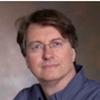
\includegraphics[width=1.0\columnwidth]{images/gregor.png}
  \caption{A demonstration in the scalability of PDF images.}
  \label{F:flow}
\end{figure}
\end{verbatim}

Which results in the following:
\begin{quote}
In Figure~\ref{F:flow} we show a black and white graph about ... .

\begin{figure}[htb]
  \includegraphics[width=1.0\columnwidth]{images/i523-overview.pdf}
  \caption{A demonstration in the scalability of PDF images.}
  \label{F:flow}
\end{figure}
\end{quote}

Note that las17graph must be a label of a valid bibtex entry. This is
needed if you have copied the image from elsewhere to avoid plagiarism.
However, if you came up with the graph yourself than you do not need a
citation.

We recommend that you place in your paper drafts all images at the which
can be done with the endfloat package

This can be enabled if you include the following lines before begin
document command:

\begin{verbatim}
\usepackage{endfloat}
\renewcommand{\efloatseparator}{\mbox{}} 

\begin{document}
\end{verbatim}

\subsection{Tables}\label{tables}
\index{Latex!Elements!tables}

Latex tables are very similar to csv table. Thus you could with
appropriate manipulation create tables from csv tables and use tools
such as spreadsheet editors to manage your table. There are even
packages that allow you to import the contents of csv tables directly
into \LaTeX.

In many cases you simply can start with an online table generator such as

\URL{https://www.tablesgenerator.com/}

For some tables you may want to rescale the width with

\begin{verbatim}
\resizebox{\textwidth}{!}{%
   ... PUT YOUR TABLE HERE ....
}
\end{verbatim}

In other cases you may want to rotate the table which you can easily
google for. In all cases use as figures, tables need to be in the
\verb|table| float environment. In contrast to figures captions are on
the top. All tables must be referred to by \verb|ref|. For more
information in directly including csv tables see 

\URL{http://mirror.utexas.edu/ctan/macros/latex/contrib/csvsimple/csvsimple.pdf}

However the format is very easy and can in most cases directly be
included in latex as shown in Table~\ref{T:elements}.

\begin{verbatim}
\begin{table}[htb]
\caption{Table with elements}\label{T:elements}
\bigskip
\begin{center}
\begin{tabular}{ c c c }
 column1  & column2  & column3 \\
\hline
\hline
 element1 & element2 & element3 \\ 
 element4 & element5 & element6 \\  
 element7 & element8 & element9 \\
\hline
\end{tabular}
\end{center}
\end{table}
\end{verbatim}

\begin{table}[htb]
\caption{Table with elements}\label{T:elements}
\bigskip
\begin{center}
\begin{tabular}{ c c c }
 column1  & column2  & column3 \\
\hline
\hline
 element1 & element2 & element3 \\ 
 element4 & element5 & element6 \\  
 element7 & element8 & element9 \\
\hline
\end{tabular}
\end{center}
\end{table}

\subsection{Labels}\label{labels}
\index{Latex!Elements!labels}

As we saw already for figures and tables it is recommended to use the
label and ref commands to refer to figure or table numbers. This applies
also to sections. Thus I can place a label after a section:

\begin{verbatim}
\section{Introduction}\label{S:introduction}
\end{verbatim}

and write elsewhere in the paper:

\begin{verbatim}
As we showcased in Section~\ref{S:introduction}
\end{verbatim}

Furthermore to conveniently distinguish sections tables and figures, we
use the prefix S T F followed by a colon for the label. This helps
organizing your paper in case you have many labels.

\subsection{Mathematics}\label{math}
\index{Latex!Elements!mathematics}

One of the strength of LaTeX thi the ability to write easily
sophisticated mathematical expressions on paper with high quality. A
good online resource is provided by the following online resource from
which we have copied some examples:

\begin{itemize}

\item
  \url{https://en.wikibooks.org/wiki/LaTeX/Mathematics}
\end{itemize}

To activate them use 

\begin{verbatim}
\usepackage{amsmath}
\end{verbatim}

at the beginning of the document after the document class

Exponents are using the \^{} character:

\begin{tcblisting}{colback=blue!5!white,colframe=gray!50!blue,listing side text,
  title=exponents,fonttitle=\bfseries}
$(a+b)^2 = a^2 + 2ab + b^{c+2}$
\end{tcblisting} 

Greek letters are referred to by their name proceeded by the slash:

\begin{tcblisting}{colback=blue!5!white,colframe=gray!50!blue,listing side text,
  title=greek,fonttitle=\bfseries}
$ \alpha \beta \gamma \Gamma \pi \Pi \phi $
\end{tcblisting}


Limits can be written as follows:

\begin{tcblisting}{colback=blue!5!white,colframe=gray!50!blue,listing side text,  title=limits,fonttitle=\bfseries}
$ \lim_{x \to \infty} \exp(-x) = 0 $
\end{tcblisting}

Fractions are indicated by the frac command, and binomials by binom:

\begin{tcblisting}{colback=blue!5!white,colframe=gray!50!blue,listing side text,  title=fraction,fonttitle=\bfseries}
$ \frac{n!}{k!(n-k)!} = \binom{n}{k} $   
\end{tcblisting}

Matrices can be created as follows:

\begin{tcblisting}{colback=blue!5!white,colframe=gray!50!blue,listing side text,  title=matrix,fonttitle=\bfseries}
$ A_{m,n} = 
\begin{pmatrix}
  a_{1,1} & a_{1,2} & \cdots & a_{1,n} \\
  a_{2,1} & a_{2,2} & \cdots & a_{2,n} \\
  \vdots  & \vdots  & \ddots & \vdots  \\
  a_{m,1} & a_{m,2} & \cdots & a_{m,n} 
\end{pmatrix} $
\end{tcblisting}



\section{Advanced topics}

\subsection{ACM and IEEE Proceedings Format}\label{acm-proceedings-format}
\index{Latex!proceedings!acm}
\index{Latex!proceedings!ieee}

\begin{figure}[!h]
  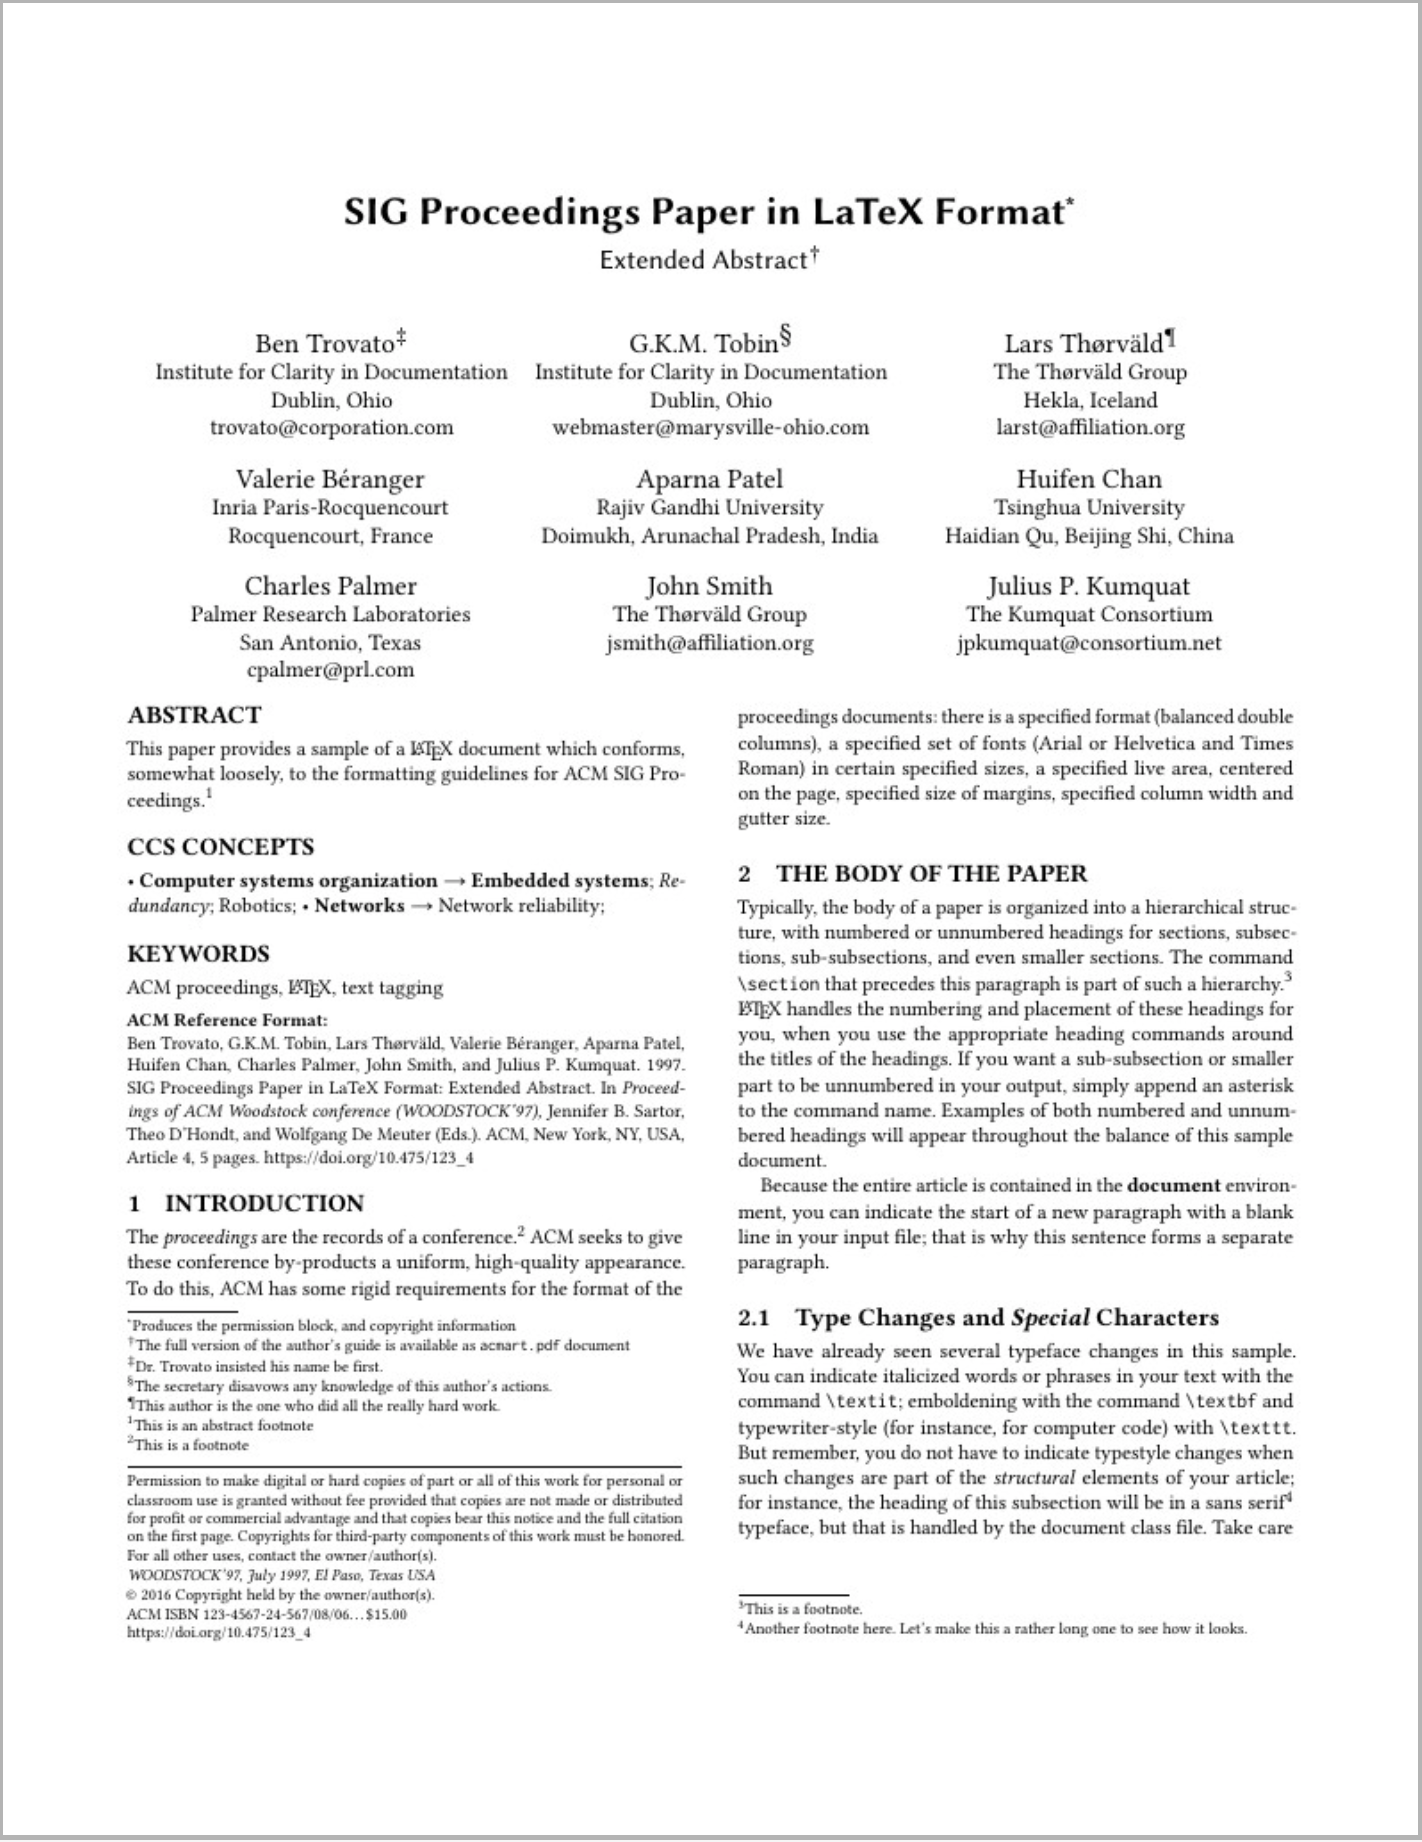
\includegraphics[width=6cm]{images/doc/acm.png}
  \hfill
  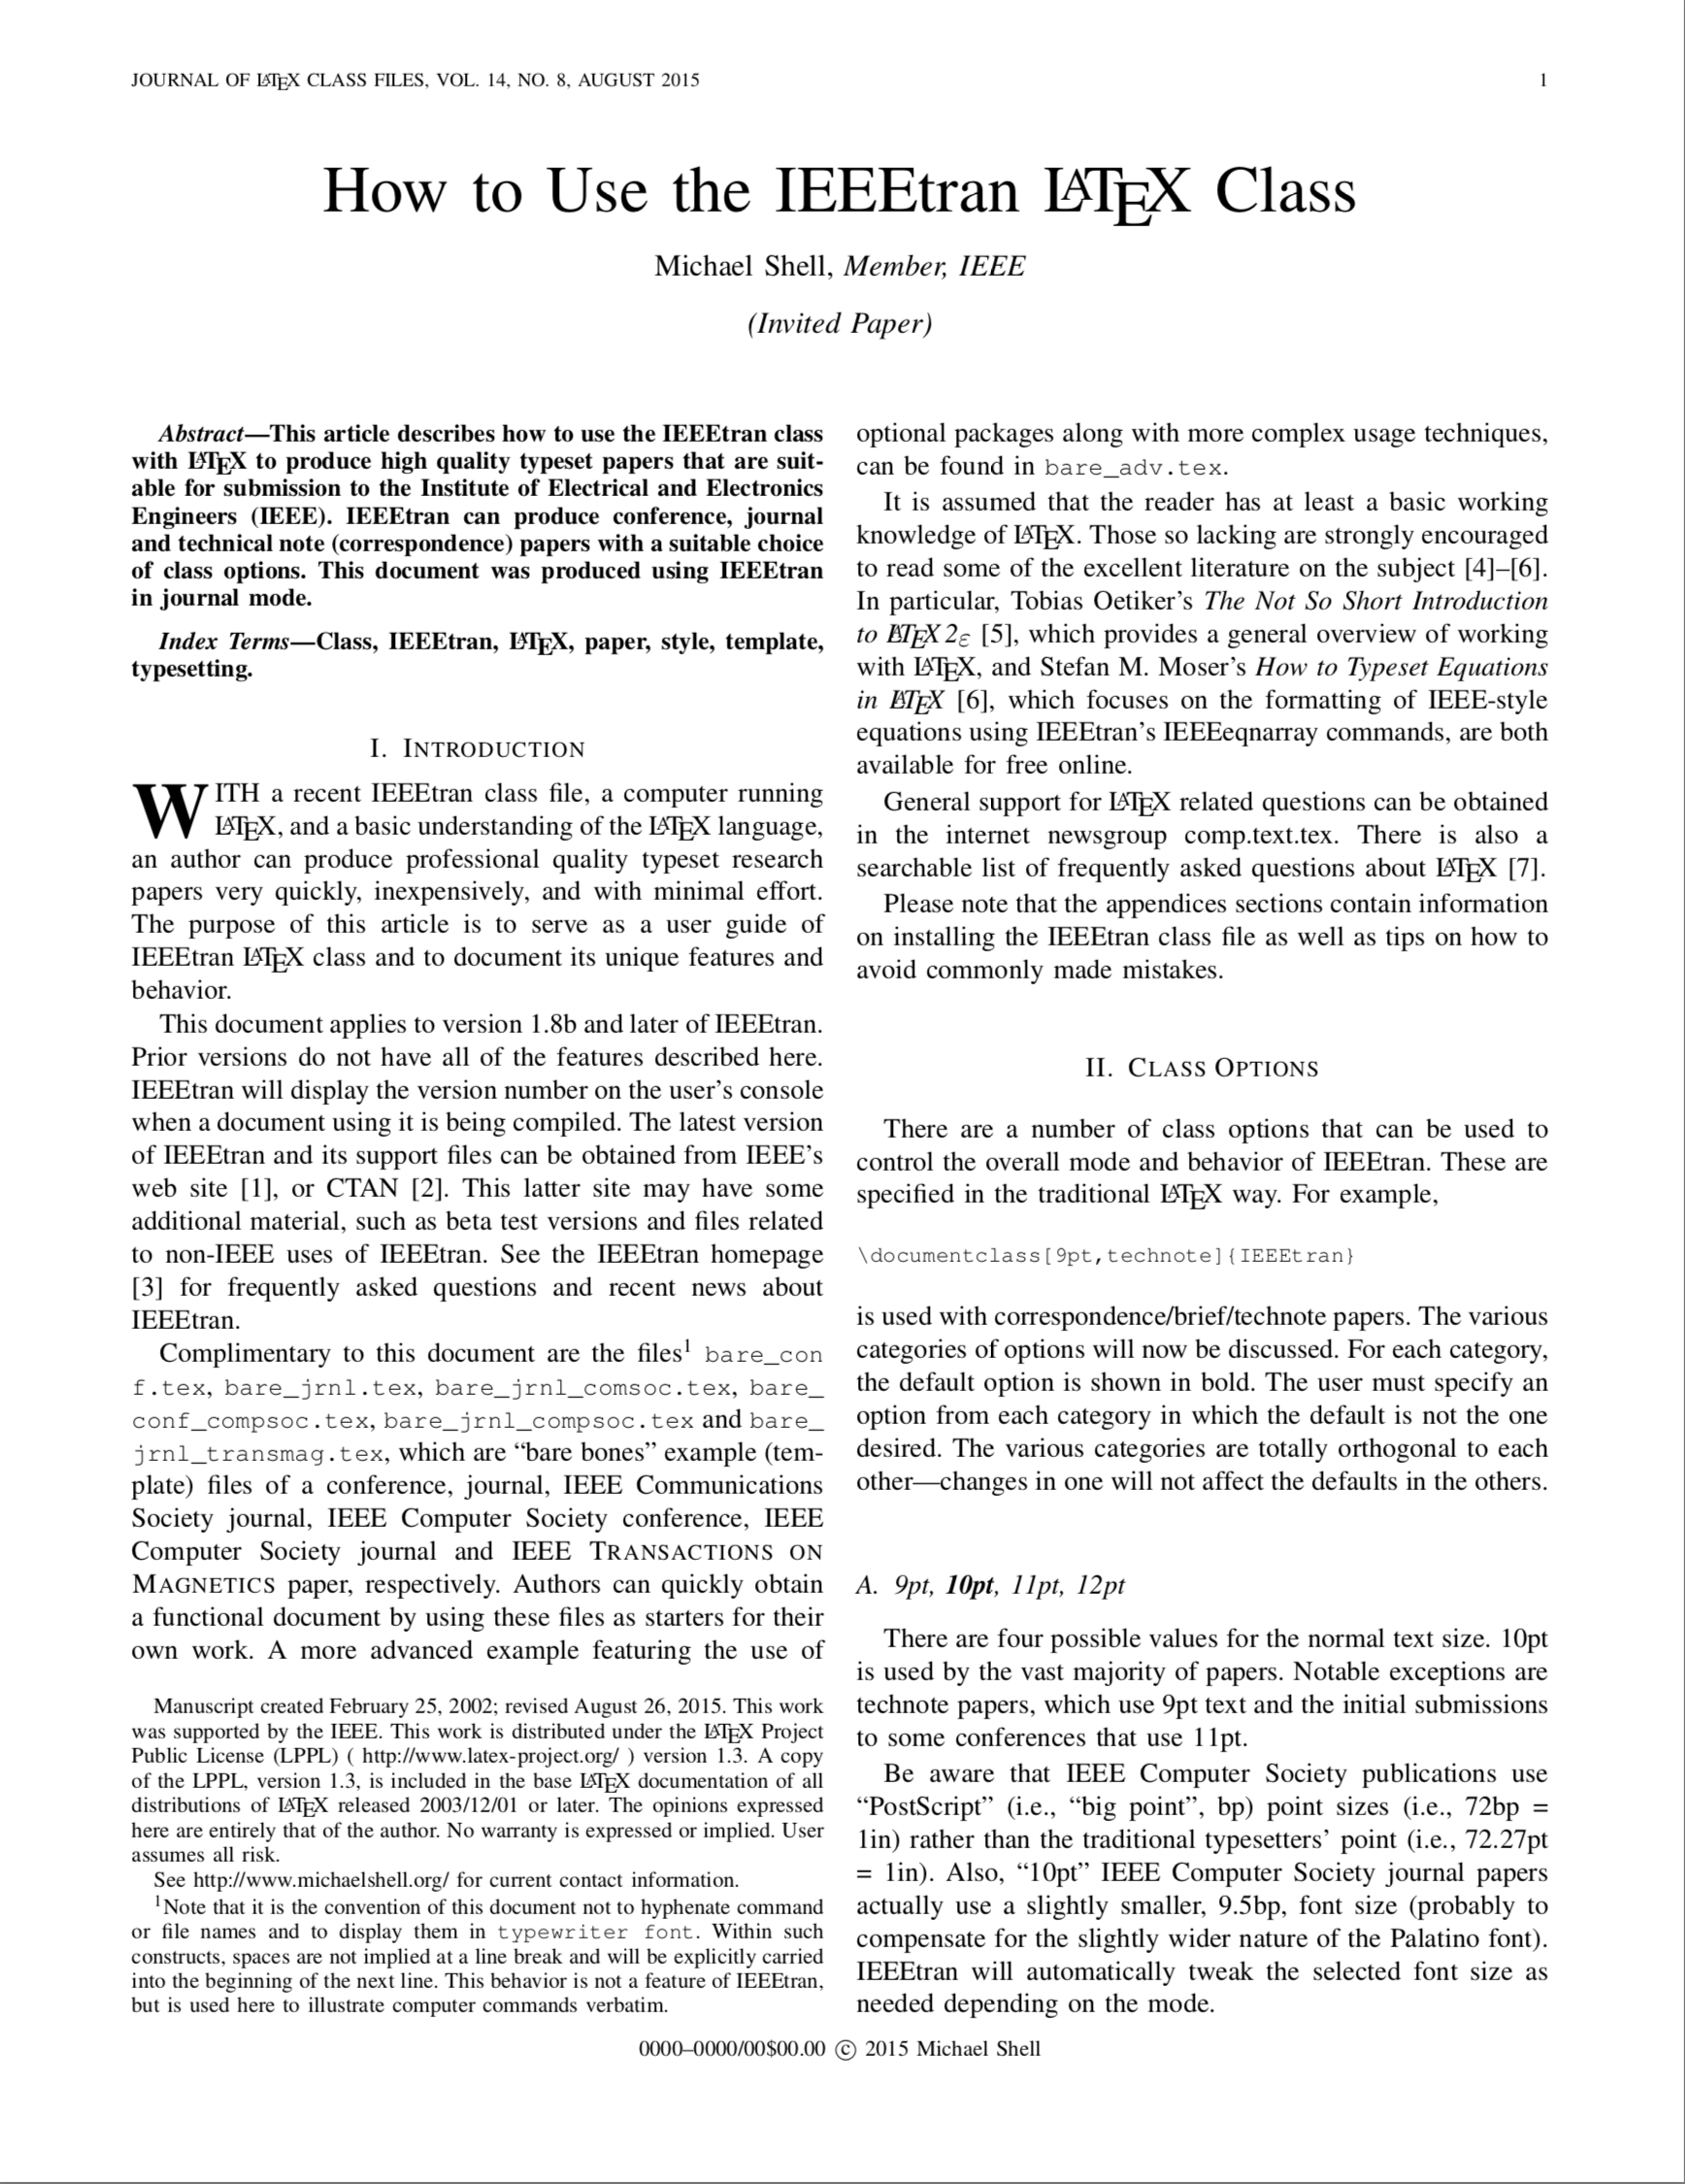
\includegraphics[width=6cm]{images/doc/ieee.png}
\caption{The look of the ACM and IEEE format templates}
\end{figure}

\begin{itemize}

\item
  \url{http://www.acm.org/publications/proceedings-template}
\item
  \url{https://www.ieee.org/conferences_events/conferences/publishing/templates.html}
\end{itemize}

\subsection{Generating and Managing Images}\label{generating-images}

To produce high quality images the programs PowerPoint and omnigraffle
on OSX are recommended. When using powerpoint please keep the image
ratio to 4x3 as they produce nice size graphics which you also can use
in your presentations. When using other rations they may not fit in
presentations and thus you may increase unnecessarily your work. We do
not recommend vizio as it is not universally available and produces
images that in case you have to present them in a slide presentation
does not easily reformat if you do not use 4x3 aspect ratio.

Naturally, graphics should be provided in SVG or PDF format so they can
scale well when we look at the final PDF. Including PNG, gif, or jpeg
files often do not result in the necessary resolution or the files
become real big. For this reason we for example can also not recommend
tools such as tablaeu as they do not provide proper exports to high
quality publication formats. For interactive display such tool may be
good, but for publications it produces inferior formatted images.

We recommend that all images be stored into a folder called images in
the same directory where your \LaTeX~ main document resides.



\subsection{Colored Boxes}

The package \verb|tcolorbox| provides sophisticated support to include
color boxes. Together with the new environment we can create nice add
ons to for example include notes.

\URL{http://osl.ugr.es/CTAN/macros/latex/contrib/tcolorbox/tcolorbox.pdf}

We have provided in this document notes as follows


\begin{tcblisting}{colback=blue!5!white,colframe=gray!50!blue,listing side text,  title=Note,fonttitle=\bfseries}
\begin{NOTE}
This is a note
\end{NOTE}
\end{tcblisting}

\begin{tcblisting}{colback=blue!5!white,colframe=gray!50!blue,listing side text,  title=Warning,fonttitle=\bfseries}
\begin{WARNING}
This is a note
\end{WARNING}
\end{tcblisting}


\subsection{Slides}\label{slides}
\index{Latex!slides}

Slides are best produced with the seminar package:

\begin{verbatim}
\documentclass{seminar}

\begin{slide}

    Hello World on slide 1

\end{slide}

The text between slides is ignored

\begin{slide}

    Hello World on slide 2

\end{slide}
\end{verbatim}

However, in case you need to have a slide presentation we recommend you
use ppt. Just paste and copy content from your PDF or your LaTeX source
file into the ppt.



\subsection{LaTeX vs. X}\label{latex-vs.-x}

We will refrain from providing a detailed analysis on why we use LaTeX
in many cases versus other technologies. In general, we find that LaTeX:

\begin{itemize}

\item
  is incredibly stable
\item
  produces high-quality output
\item
  is platform independent
\item
  has lots of templates
\item
  has been around for many years so it works well
\item
  removes you from the pain of figure placements
\item
  focusses you on content rather tan the appearance of the paper
\item
  integrates well with code repositories such as git to write
  collaborative papers.
\item
  has superior bibliography integration
\item
  has a rich set of tools that make using LaTeX easier
\item
  authors do not play with layouts much so papers in a format are
  uniform
\end{itemize}

In case you need a graphical view to edit LaTeX or LateX exportable
files you also find AucTeX and Lyx.

\subsubsection{Word}\label{word}

Word is arguably available to many, but if you work on Linux you may be
out of luck. Also Word often focusses not on structure of the text but
on its appearance. Many students abuse Word and the documents in Word
become a pain to edit with multiple users. Recently Microsoft has
offered online services to collaborate on writing documents in groups
which work well. Integration with bibliography managers such as endnote
or Mendeley is possible.

However, we ran into issues whenever we use word:

\begin{itemize}

\item
  Word tends sometimes to crash for unknown reasons and we lost a lot of
  work
\item
  Word has some issues with the bibliography managers and tends to crash
  sometimes for unknown reasons.
\item
  Word is slow with integration to large bibliographies.
\item
  Figure placement in Word in some formats is a disaster and you will
  spend many hours to correct things just to find out that if you make
  small changes you have to spend additional many hours to get used to
  the new placement. We have not yet experienced a word version where we
  have not lost images. Maybe that has changed, so let us know
\end{itemize}

However, we highly recommend the collaborative editing features of Word
that work on a paragraph and not letter level. Thus saving is essential
so you do not block other people from editing the paragraph.

\subsubsection{Google Docs}\label{google-docs}

Unfortunately, many useful features got lost in the new google docs.
However, it is great to collaborate quickly online, share thoughts and
even write your latex documents together if you like (just copy your
work in a file offline and use latex to compile it ;-) )

The biggest issue we have with Google Docs is that it does not allow the
support of 2 column formats, that the bibliography integration is
non-existent and that paste and copy from web pages and images
encourages unintended plagiarism when collecting information without
annotations (LaTeX and Word are prone to this too, but we found from
experience that it tends to happen more with Google docs users.

\subsubsection{A Place for Each}\label{a-place-for-each}

When looking at the tools we find a place for each:

\begin{description}
\item[Google docs:]
Short meeting notes, small documents, quick online collaborations to
develop documents collaboratively at the same time.
\item[Word:]
Available to many, supports 2 column format, supports paragraph based
collaborative editing, Integrates with bibliography managers.
\item[LaTeX:]
Reduces failures, great offline editing, superior bibliography
management, superior image placement, runs everywhere. Great
collaborative editing with sharelatex, allows easy generation of
proceedings written by hundreds of people with shared index.
\item[The best choice for your class:]
LaTeX
\end{description}

\section{Editing}\label{editing}

\subsection{Emacs}\label{emacs}

The text editor emacs provides a great basis for editing TeX and LaTeX
documents. Both modes are supported. In addition there exists a color
highlight module enabling the color display of LaTeX and TeX commands.
On OSX aquaemacs and carbon emacs have build in support for LaTeX. Spell
checking is done with flyspell in emacs.

\subsubsection{Aquamacs}

Aquamacs is an editor based on GNU Emacs that runs on OSX and
integrates with the OSX desktop. This is for many the preferred editor
on OSX for \LaTeX.

\url{http://aquamacs.org}

\begin{figure}[!htb]
  \centering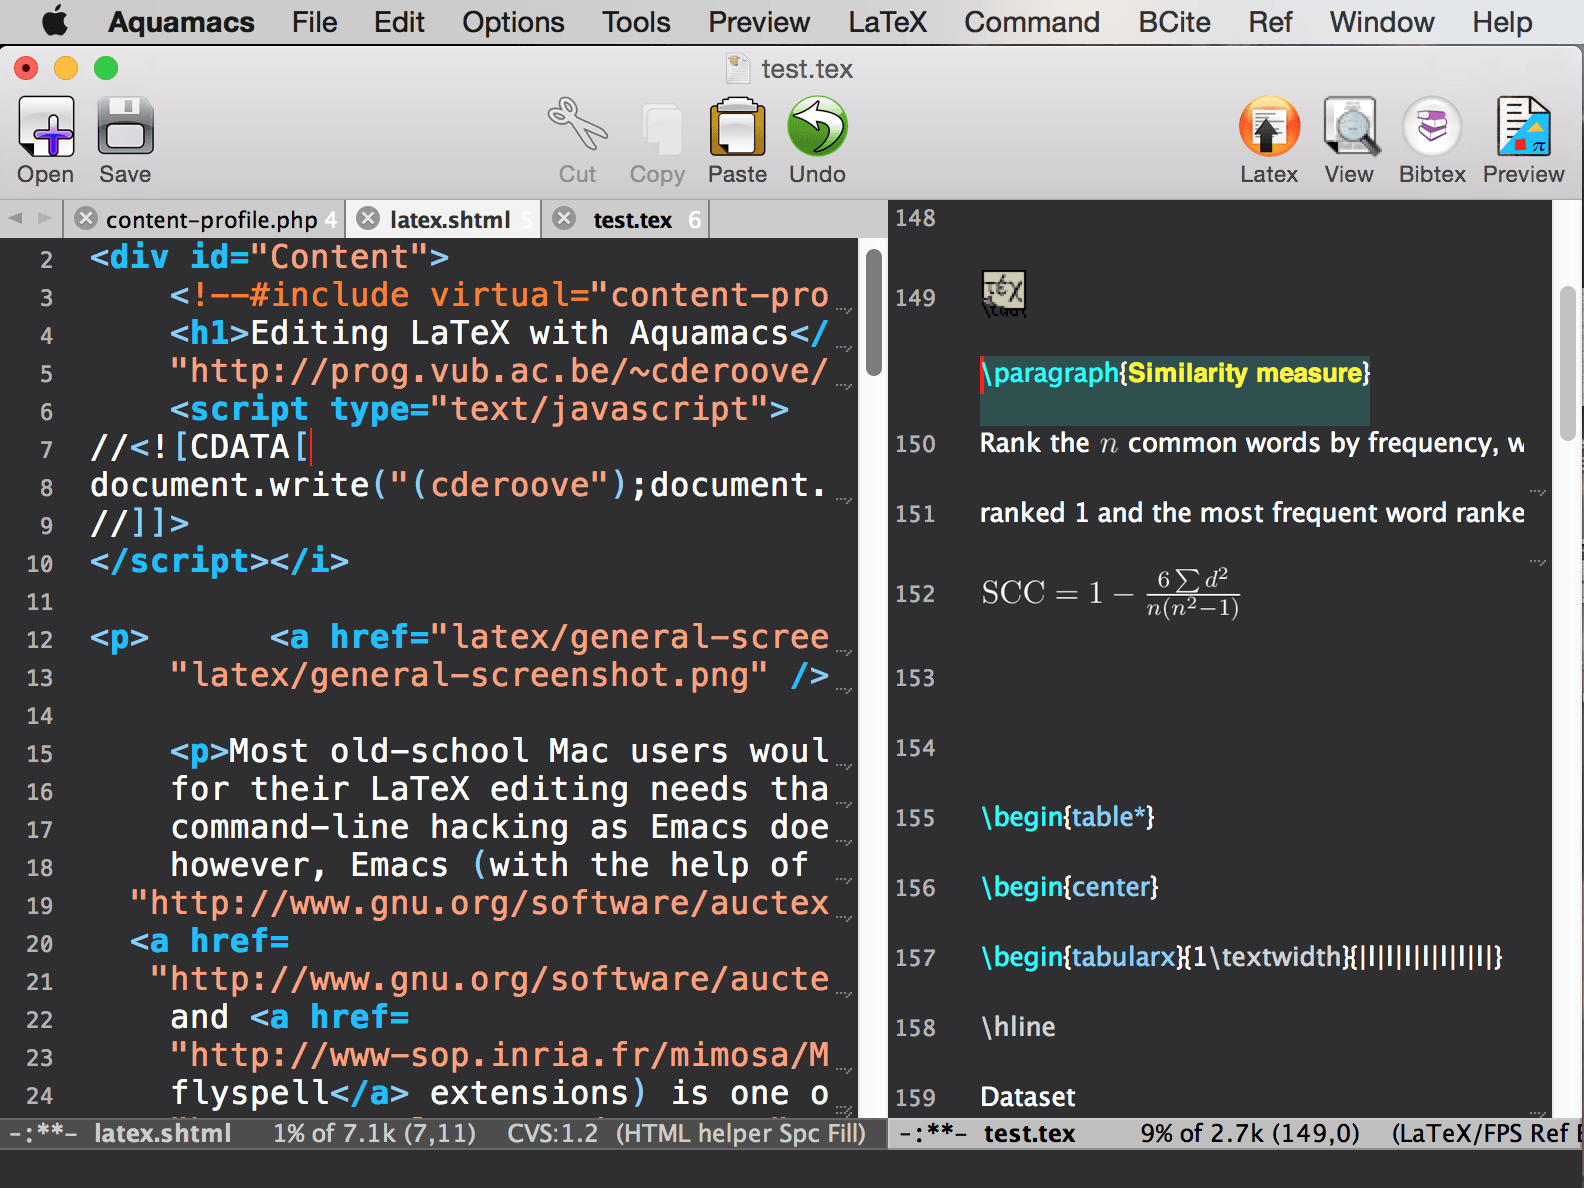
\includegraphics[width=8cm]{images/aquamacs.png}
  \caption{Aquamacs}
  \label{F:aquamacs}
\end{figure}


\subsection{Vi/Vim}\label{vivim}

Another popular editor is vi or vim. It is less feature rich but many
programmers ar using it. As it can edit ASCII text you can edit LaTeX.
With the LaTeX add-ons to vim, vim becomes similar powerful while
offering help and syntax highlighting for LaTeX as emacs does. (The
authors still prefer emacs)

\subsection{TeXshop}\label{texshop}

Other editors such as TeXshop are available which provide a more
integrated experience. However, we find them at times to stringent and
prefer editors such as emacs.

\subsection{LyX}\label{lyx}

We have made very good experiences with Lyx. You must assure that the
team you work with uses it consistently and that you all use the same
version.

\begin{figure}[!htb]
  \centering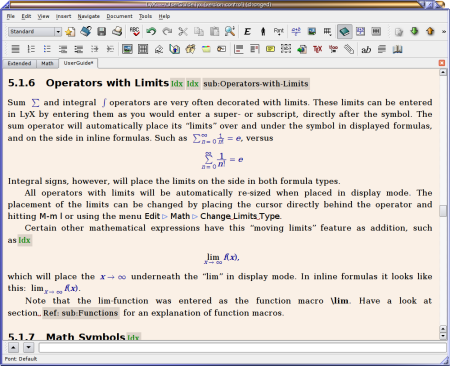
\includegraphics[width=8cm]{images/lyx.png}
  \caption{Lyx}
  \label{F:lyx}
\end{figure}

Using the ACM templates is documented here:

\begin{itemize}

\item
  \url{https://wiki.lyx.org/Examples/AcmSiggraph}
\end{itemize}

On OSX it is important that you have a new version of LaTeX and Lyx
installed. As it takes up quite some space, you ma want to delete older
versions. The new version of LyX comes with the acmsigplan template
included. However on OSX and other platforms the .cls file is not
included by default. However the above link clearly documents how to fix
this.

\subsection{WYSIWYG locally}\label{wysiwyg-locally}

We have found that editors such as Lyx and Auctex provide very good
WYSIWYG alike features. However, we found an even easier way while using
skim, a pdf previewer, in conjunction with emacs and latexmk. This can
be achieved while using the following command assuming your latex file
is called `report.tex`:

\begin{verbatim}
latexmk -pvc -view=pdf report
\end{verbatim}

This command will update your pdf previewer (make sure to use skim)
whenever you edit the file report.tex and save it. It will maintain via
skim the current position, thus you have a real great way of editing in
one window, while seeing the results in the other.

Skim can be found at: \url{http://skim-app.sourceforge.net/}

\subsection{Markdown and \LaTeX}
\index{Latex!markdown}

It may come as a surprise to many that one can actually write simple
LaTeX documents also in markdown Syntax or mix section written in
markdown while others are written in LaTeX. To do so all you ahve to
do is place the markdown text in a separate file. Let us call the file 
\verb|content.md| which has the following lines included in it:

\begin{verbatim}
# Section

* item a
* item b
\end{verbatim}

Obviously, we would have to convert this to LaTeX. Luckily there is a
very useful program called \textit{pandoc} that does this for you. YOu
could make the translation in the shell, but you could also make the
translation locally on your computer while allowing \LaTeX~ to start up
external programs. This is achieved with the \textit{write18} command and
allowing LaTeX explicitly to call external programs. Please inspect
the following latex file that includes a template on how to do
this. We assume the file is called markdown.tex for our example.

\begin{verbatim}
\documentclass{article}

\include{graphicx}
\newcommand{\tightlist}{}

\begin{document}
\immediate\write18{pandoc content.md -o content.tex}

\input{content}

\end{document}
\end{verbatim}

Now to generate the PDF we simply have to call the following command
that include the \textit{-shell-escape} flag to allow the execution of
write18 embedded commands:

\begin{verbatim}
pdflatex -shell-escape markdown-test
\end{verbatim}

The output will be \textit{markdown.pdf} with the content from the
markdown file translated. Doing this naturally allows you to write
large portions in markdown and automatically include them in your
LaTeX document. Hence, you can use editors such as Macdown to initially
work in semi WYSIWYG mode and do fairly straight forward
edition. Naturally the same can be done in RST. Naturally the most
elementary features are supported. For more sophisticated features,
please use LaTeX directly.


\subsection{Including RST into LaTeX}

content.rst:

\begin{verbatim}
Section
-------

* item a
* item b
\end{verbatim}

sample.tex:

\begin{verbatim}
\documentclass{article}

\include{graphicx}
\newcommand{\tightlist}{}

\begin{document}
\immediate\write18{pandoc content.rst -o content.tex}

\input{content}

\end{document}
\end{verbatim}


\subsection{pyCharm}

TODO: comment on how we can use pycharm for editing and what the
limitations are.

\subsection{MSWord}

it is possible to use Word.

be careful with 

\section{The LaTeX Cycle}\label{the-latex-cycle}
\index{Latex!cycle}

To create a PDF file from latex yo need to generate it following a
simple development and improvement cycle.

First, Create/edit ASCII source file with \texttt{file.tex} file:

\begin{verbatim}
emacs file.tex
\end{verbatim}

Create/edit bibliography file:

\begin{verbatim}
jabref refs.bib
\end{verbatim}

Create the PDF:

\begin{verbatim}
pdflatex file
bibtex file
pdflatex file
pdflatex file
\end{verbatim}

View the PDF:

\begin{verbatim}
open file
\end{verbatim}

It not only showcases you an example file in ACM 2 column format, but
also integrates with a bibliography. Furthermore, it provides a sample
Makefile that you can use to generate view and recompile, or even
autogenerate. A compilation would look like:

\begin{verbatim}
make
make view
\end{verbatim}

If however you want to do things on change in the tex file you can do
this automatically simply with:

\begin{verbatim}
make watch
\end{verbatim}

for make watch its best to use skim as pdf previewer


\section{Tips}\label{tips}

Including figures over two columns:

\begin{itemize}
\item
  \url{http://tex.stackexchange.com/questions/30985/displaying-a-wide-figure-in-a-two-column-document}
\item
  positioning figures with textwidth and columnwidth
  \url{https://www.sharelatex.com/learn/Positioning_images_and_tables}
\item
  An organization as the author. Assume the author is National Institute
  of Health and want to have the author show up, please do:

\begin{verbatim}
key= {National Institute of Health},
author= {{National Institute of Health}},
\end{verbatim}

  Please note the \{\{ \}\}
\item
  words containing `fi' or `ffi' showing blank places like below after
  recompiling it: find as nd efficiency as e ciency

  You copied from word or PDF ff which is actually not an ff, but a
  condensed character, change it to ff and ffi, you may find other such
  examples such as any non ASCII character. A degree is for example
  another common issue in data science.
\item
  do not use \textbar{} \& and other latex characters in bibtex
  references, instead use , and the word and
\item
  If you need to use \_ it is \_ but if you use urls leave them as is
\item
  We do recommend that you use sharelatex and jabref for writing papers.
  This is the easiest solution and beats in many cases MSWord as you can
  focus on writing and not on formatting.
\end{itemize}

\subsection{Colorful Output}

Instead of using pdflatex, you can also install \verb|pydflatex| that
provides a convenient wrapper and colorizes the output while
eliminating a lot of warnings that you may initially not want to deal
with. To install it please use:

\begin{verbatim}
pip install blessings
pip install -e "git+https://github.com/olivierverdier/pydflatex#egg=pydflatex"
\end{verbatim}

You can see the manual page with 

\begin{verbatim}
pydflatex --help

usage: usage: pydflatex [options] texfile1

Compile a tex file with pdflatex and make the auxiliary files invisible. Note
that the '.tex' extension may be omitted

positional arguments:
  tex path            path to tex file

optional arguments:
  -h, --help          show this help message and exit
  -o, --open          view the pdf file(s) in a pdf viewer.
  -k, --continue      continue on error
  -w, --with-warning  do not suppress common warnings
  -v, --verbose       Verbose output for debugging
  -p, --plain         No coloured output
  -x, --xetex         Use XeLaTeX engine
  -l, --log-parsing   Only parse log
  -t, --typesetting   Only typeset
\end{verbatim}

\subsection{latex2html}

\LaTeX~ can be exported to html with the the tool
\verb|latex2html|. It is available 

for Linux and OSX. More information can be found at

\URL{http://mirrors.ctan.org/support/latex2html/manual.pdf}

\URL{www.latex2html.org}

\begin{WARNING}
At this time the inastallation via brew install of latex2html is
broken. Instead one needs to conduct the insalation from source.

\begin{verbatim}
brew install latex2html
\end{verbatim}
\end{WARNING} 

The instalation from source can be conducted as follows

\begin{verbatim}
brew install libpng
wget https://github.com/latex2html/latex2html/archive/master.zip
uzip master.zip 
cd latex2html-master/
configure
make
make check
sudo make install
\end{verbatim}

\subsection{lachek}
\label{s:lacheck}
\index{lacheck}
\index{\LaTeX!lacheck}

Lacheck allows to find­ing common mistakes in \LaTeX~
documents. We recommend that you use it to check your latex files.

You can invoke it as follows

\begin{lstlisting}
lacheck filename.tex
\end{lstlisting}

More information can be found at

\URL{https://ctan.org/tex-archive/support/lacheck}

\subsection{chktex}
\label{s:chktex}
\index{chktex}
\index{\LaTeX!chktex}

LaTeX is a powerfull program to develop professional documents. In
some cases i is useful to check some semantics on the document. For
this reason you can use 

\begin{lstlisting}
chktex filename.tex
\end{lstlisting}

It will execute a number of filters and produce a check on them. You
can configure it to produce warnings and errors based on the error
type.

For a manual page use

\begin{lstlisting}
chktex --help
\end{lstlisting}

When using it some errors and wrnings can be ignored, while others
should be considerd. Supported featured mantiond on the Web page
include:
``
\begin{itemize}
          \item  Commands terminated with space. Ignores \verb|\tt|, etc.
          \item  Space in front of references instead of \verb|~|.
          \item  Forgetting to group parenthesis characters when
            sub-/superscripting.
          \item  Italic correction (\verb|\/|) mistakes (double, missing,
            unnecessary).
          \item  Parenthesis and environment matching.
          \item  Ellipsis detection; also checks whether to use \verb|\dots|,
            \verb|\cdots| or \verb|\ldots|.
          \item  Enforcement of normal space after abbreviation. Detects most
            abbreviations automagically.
          \item  Enforcement of end-of-sentence space when the last sentence
            ended with capital letter.
          \item  Math-mode on/off detection.
          \item  Quote checking, both wrong types (\verb|"|) and wrong direction.
          \item  Recommends splitting three quotes in a row.
          \item  Searching for user patterns.
          \item  Displays comments.
          \item  Space in front of \verb|\label| and similar commands.
          \item  Use of \verb|x| instead of \verb|$\times$| between numbers.
          \item  Multiple spaces in input which will be rendered as one space
            (or multiple spaces, where that is undesirable).
          \item  Warns about text which may be ignored.
          \item  Mathematical operators typeset as variables.
          \item  No space in front of/after parenthesis.
          \item  Demands a consistent quote style.
          \item  Punctuation inside inner math mode/outside display math mode.
          \item  Use of TeX primitives where LaTeX equivalents are available.
          \item  Space in front of footnotes.
          \item  Bogus characters following commands.
\end{itemize}
``

For more details see

\URL{http://baruch.ev-en.org/proj/chktex/}

\subsection{References}
\index{Latex!other documentation}

\begin{description}


\item[Latex Sheet:]    \url{https://wch.github.io/latexsheet/latexsheet.pdf}

\item[Latex Short:]    \url{http://tug.ctan.org/info/lshort/english/lshort.pdf}

\item[Wikibook:]       \url{https://en.wikibooks.org/wiki/LaTeX}
\item[Wikibook (PDF)]: \url{https://upload.wikimedia.org/wikipedia/commons/2/2d/LaTeX.pdf}

\item [Links to books:] \url{https://latexforhumans.wordpress.com/2008/10/11/the-best-guides-to-latex/}
\item [Links to books:] \url{https://www.latex-project.org/help/books/}
\item [LaTeX2e:]
  The
  \href{http://texdoc.net/texmf-dist/doc/latex/latex2e-help-texinfo/latex2e.pdf}{LaTeX
  Reference Manual} provides a good introduction to Latex.

\end{description}


\begin{itemize}

\item
  LaTeX Users and Reference Guide, by Leslie Lamport
  \url{https://www.amazon.com/LaTeX-Document-Preparation-System-2nd/dp/0201529831/ref=sr_1_2?s=books\&ie=UTF8\&qid=1507114870\&sr=1-2\&keywords=lamport}
\item
  LaTeX an Introduction, by Helmut Kopka
  \url{https://www.amazon.com/Guide-LaTeX-4th-Helmut-Kopka/dp/0321173856/ref=pd_lpo_sbs_14_t_0?_encoding=UTF8\&psc=1\&refRID=2BB4APDFEX34A4JM65ZB}
\item
  The LaTeX Companion, by Frank Mittelbach
  \url{https://www.amazon.com/LaTeX-Companion-Techniques-Computer-Typesetting/dp/0201362996}
\end{itemize}



\chapter{Managing Bibliographies}

\FILENAME

\section{Integrating Bibliographies}
\label{S:bibliographies}
\index{Bibliography}
\index{bibtex}
\index{biber}

Bibliography management in \LaTeX\ is one of the many features that
motivate many researchers to make \LaTeX the tool of choice to write
academic papers. There are numerous bibliography styles available that
allow easy adaptation to differen journal and proceedings style. As
such, it includes styles for bibliographies formated in ACM and IEEE
style.

\subsection{biber}

\TODO{Describe use of biber instead of bibtex}

\subsection{bibtex}

This section assumes we use the standard bibtex program to integrate
citations into a \LaTeX\ paper.

An example to use the IEEE style for a paper includes to set
the style to IEEEtran before you add the reference:

\begin{verbatim}
\bibliographystyle{IEEEtran}
\bibliography{references.bib}
\end{verbatim}

To properly create PDF papers which using bibtex, we have to make sure
that all indexes, citations, references and labels are updated. This
is done with the help of the following commands assuming your file is
called \verb|file.tex|

\begin{verbatim}
pdflatex  file
bibtex file
pdflatex  file
pdflatex  file
\end{verbatim}


\begin{IU}
At IU you are required to use our template. which includes a Makefile
and either calls the above three commands or used latexmk
\end{IU}

The reason for the multiple execution of the latex program is to update
all cross-references correctly. In case you are not interested in
updating the library every time in the writing progress just postpone it
till the end. Missing citations are viewed as {[}?{]}.

Two programs stand out when managing bibliographies: emacs and jabref:

  \URL{http://www.jabref.org/}

Other programs such as Mendeley, Zotero, and even endnote integrate with
bibtex. However their support is limited, so we recommend that you just
use jabref as it is free and runs on all platforms.

\subsection{jabref}\label{jabref}

\TODO{Tyler: include cite for jabref, bibtex, biber at appropriate
  location in this section. Add them to the bib file.}

Practical experience with many generations of students shows that
\textit{jabref} is a very simple to use bibliography manager for LaTeX and
other systems. It can create a multitude of bibliography file formats
and allows upload in other online bibliography managers.

For information on how to install and use jabref please go to 
\url{http://www.jabref.org/}. There you will find the appropriate
download link.

We provide also a convenient video on how to use jabref and show
several methods on how to add entries easily to your bibliography database.

\video{Bibliography}{1:41}{jabref}{https://youtu.be/QVbifcLgMic}



\section{Entry types}

In this section we will explain how to find and properly generate
bibliographic entries. We are using bibtex for this as it is easy to
use and generates reasonable entries that can be included in
papers. What we like to achieve in this section is not to just show
you a final entry, but to document the process on how that entry was
derived. This will allow you to replicate or learn from the process to
apply to your own entries. As part of this we copy and paste
information found via Web searches.

We will address a number of important reference types which includes:

\begin{itemize}

\item
  wikipedia entries
\item
  github (see Section~\ref{s:e:source-code-references})
\item
  books
\item
  articles in a scientific journal (see Section~\ref{s:e:article-in-a-journal})
\item
  articles in a conference (see Section~\ref{s:e:article-in-a-conference-proceedings})
\item
  articles in magazines (non scientific)
\item
  blogs
\end{itemize}

\subsection{Source Code References}
\label{s:e:source-code-references}
\index{Bibtex!Source code}

Often, we need to cite a source code from a publicly hosted
repository. Such repositories are frequently used and include, for
example github, bitbucket, sourceforge, or your Universities code
repository as long as it is publicly reachable. As changes can occur on
these repositories, it is important that the date of access is listed in
the entry or even the release version of the source code.

Let us without bias chose a random source dode entry that has been
contributed by a student as follows:

\begin{verbatim}
@Misc{gonzalez_2015,
  Title =  {Buildstep},
  Author =     {Gonzalez, Jose and Lindsay, Jeff},
  HowPublished = {Web Page},
  Month =  {Jul},
  Note =   {Accessed: 2017-1-24},
  Year =   2015,
  Key =        {www-buildstep},
  Url =        {https://github.com/progrium/buildstep}
}
\end{verbatim}

Is this entry correct? Let us analyse. But first we need to undersrand
the semantics of the fields.

\subsubsection{What are the Different entry Types and Fields}

You see that the entry contains a number of fields. An extensive
explanation of these fields can be found at 

Please see \url{https://en.wikipedia.org/wiki/BibTeX}

We provide for this example a comprehensive discussions of the fields
used. For other examples we suggest you refer to the document to
identify what needs to be filled out.

\subsubsection{Entry type Misc}\label{s:e:entry-type-misc}
\index{Bibtex!Field!Misc}

First, it seems appropriate to use a \emph{@misc} entry. We correctly
identify this is a misc entry as it is online available. More recent
version of bibtex include also the type \emph{@online} for it. However,
in order to maintain compatibility to older formats we chose simply Misc
here and if we really would need to we could replace it easily.

\subsubsection{Label}\label{s:e:label}
\index{Bibtex!Field!Label}

Typically the bibliography label should contain 3 letters from an
author name, short year and the short name of the publication to
provide maximum information regarding the publication. However in this
case the project is hosted on github, so creating the label based on
just the github location seems more logical. Thus our label that we
propose is given by 

\verb|github-progrium-buildstep|


Under no circumstances should you use underscores as they can have unintended
consequences in programs we use to create papers for our classes. Just
use a minus sign instead. As it is hosted on github we also want the
githubname and the projectname. As you can see we just derived it from
the URL.

\begin{IU}
When managing bibliography entries with large numbers of collaborators
it is advisable that all bibliography labels be initially be prefixed
with an id for the collaborator. In our case we use the HID. Thus in
our case we will have the following label.

\verb|hid-sp18-000-github-progrium-buildstep|

\end{IU}


\subsubsection{Author}\label{s:e:author}
\index{Bibtex!Field!Author}

Normally we can write in the author fiels the names of the authors
separated by the work and. IT is important tu use the word \verb|and|
but not use a comma. However, this only works if the lastname does not
contain a space in it. In order to avoid confusing the system, we
recommend therefore to write all names in the form
\verb|Lastname, Firstname Middle Initials|

Thus we find in our example

\verb|  Author =     {Gonzalez, Jose and Lindsay, Jeff},|

\begin{WARNING}
Please note the word and between authors. and not a comma, commas are
only used to distinguish between lastname and firstname.
\end{WARNING}


\subsubsection{Key}\label{s:e:key}
\index{Bibtex!Field!Key}

In this case the key field can be removed as the entry has an author
field entry. If there was no author field, we use the key to specify
the alphabetical ordering based on the specified key. Note that a key is
not the label. In fact in our original entry the key field was wrongly
used and the student did not understand that the key is used for
sorting.

\subsubsection{Howpublished}\label{s:e:howpublished}
\index{Bibtex!Field!Howpublished}

Since the source is a github project repository, the howpublished field
shall hold the value \verb|{Code Repository}|. If the
url specified was a normal webpage, the \verb|{Web Page}| entry would be
valid.

\subsubsection{Month}\label{s:e:month}
\index{Bibtex!Field!Month}

To allow internationalization of the month we use the first 3 letters
in the english language for the month. Thus it is 
\verb|month = jul|. Note that there are no brackets around the month.

\subsubsection{Owner}\label{s:e:owner}
\index{Bibtex!Field!Owner}

In class we introduced the convention to put the student HID in it. If
multiple students contributed, add them with space separation.

\subsubsection{Accessed}\label{s:e:accessed}
\index{Bibtex!Field!Accessed}

As some styles do not support the accessed field, we simply include it in
the note field. This is absolutely essential as code can change and when
we read the code we looked at a particular snapshot in time. In addition
it is often necessary to record the actual version of the code or the branch.
Typically for github entries, it is best to just use the month and
year field as some styles check for it.

\subsubsection{Final Entry}

Filling out as many fields as possible with information for this entry
we get:

\begin{verbatim}
@Misc{github-progrium-buildstep,
  Title =  {Buildstep},
  Author =     {Jose Gonzalez and Jeff Lindsay},
  HowPublished = {Code Repository},
  Year =   {2015},
  Month =  jul,
  Note =   {Accessed: 2017-1-24, master branch},
  Url =    {https://github.com/progrium/buildstep},
  Owner =  {S17-IO-3025},
}
\end{verbatim}

We are using the release date in the year and month field as this
project uses this for organizing releases. However, other project may
have release versions so you would have in addition to using the data
also to include the version in the note field such as:

\begin{verbatim}
Note =     {Version: 1.2.3, Accessed: 2017-1-24},
\end{verbatim}


\subsection{Pedigree}

Often it is advantageous to document the pedigree of the bibtex
entries. Eg, how did you derive the final entry? To do so you can
simply add a field such as \verb|bibsource| and include in it all
links you used to gather the final entry. However, we believe that the
effort to curate an entry is sufficient to manage your own
bibliography which you should freely distribute and constitute an own
contribution. 

\subsection{Article in a Journal}
\label{s:e:article-in-a-journal}
\index{Bibtex!Article}

Many online bibtex entries that you will find are wrong or
incomplete. Often you may find via google a bibtex entry that may need
some more research. Let us assume your first google query returns a
publication and you cite it such as this:

\begin{verbatim}
@Unpublished{unpublished-google-sawzall,
    Title = {{Interpreting the Data: Parallel Analysis with Sawzall}},
    Author = {{Rob Pike, Sean Dorward, Robert Griesemer, Sean Quinlan}},
    Note = {accessed 2017-01-28},
    Month = {October},
    Year = {2005},
    Owner = {for the purpose of this discussion removed},
    Timestamp = {2017.01.31}
}
\end{verbatim}

Could we improve this entry to achieve your best? We observe:

\begin{enumerate}
\item
  The author field has a wrong entry as the , is to be replaced by an
  and.
\item
  The author field has authors and thus must not have a \{\{ \}\}
\item
  The url is missing, as the simple google search actually finds a PDF
  document.
\end{enumerate}

Let us investigate a bit more while searching for the title. We find

\begin{enumerate}
\def\labelenumi{\Alph{enumi})}
\item
  \url{https://www.google.com/url?sa=t\&rct=j\&q}=\&esrc=s\&source=web\&cd=1\&ved=0ahUKEwj\_ytSA-PDRAhUH8IMKHaomC-oQFggaMAA\&url=https\%3A\%2F\%2Fresearch.google.com\%2Farchive\%2Fsawzall-sciprog.pdf\&usg=AFQjCNHSSfKBwbxVAVPQ0td4rTjitKucpA\&sig2=vbiVzi36B3gGFjIzlUKBDA\&bvm=bv.146073913,d.amc
\item
  \url{https://research.google.com/pubs/pub61.html}
\item
  \url{http://dl.acm.org/citation.cfm?id=1239658}
\end{enumerate}

Let us look at A)

As you can see from the url this is actually some redirection to a google
web page which probably is replaced by B as its from google research. So
let us look at B)

Now when you look at the link we find the url
\url{https://research.google.com/archive/sawzall-sciprog.pdf} which
redirects you to the PDF paper.

When we go to B) we find surprisingly a bibtex entry as follows:

\begin{verbatim}
@article{61,
  title = {Interpreting the Data: Parallel Analysis with Sawzall},
  author = {Rob Pike and Sean Dorward and Robert Griesemer and Sean Quinlan},
  year = 2005,
  URL = {https://research.google.com/archive/sawzall.html},
  journal = {Scientific Programming Journal},
  pages = {277--298},
  volume = {13}
}
\end{verbatim}

Now we could say let us be satisfied, but C) seems to be even more
interesting as its from a major publisher. So lats just make sure we
look at C)

If you go to C, you find under the colored box entitled Tools and
Resources a link called \textbf{bibtex}. Thus it seems a good idea to
click on it. This will give you:

\begin{verbatim}
@article{Pike:2005:IDP:1239655.1239658,
    author = {Pike, Rob and Dorward, Sean and Griesemer, Robert and Quinlan, Sean},
    title = {Interpreting the Data: Parallel Analysis with Sawzall},
    journal = {Sci. Program.},
    issue_date = {October 2005},
    volume = {13},
    number = {4},
    month = oct,
    year = {2005},
    issn = {1058-9244},
    pages = {277--298},
    numpages = {22},
    url = {http://dx.doi.org/10.1155/2005/962135},
    doi = {10.1155/2005/962135},
    acmid = {1239658},
    publisher = {IOS Press},
    address = {Amsterdam, The Netherlands, The Netherlands},
}
\end{verbatim}

Now we seem to be at a position to combine our search result as neither
entry is sufficient. As the doi number properly specifies a paper (look
up what a doi is) we can replace the url with one that we find online,
such as the one we found in A) Next we see that all field sin B are
already covered in C, so we take C) and add the url. Now as the label is
great and uniform for ACM, but for us a bit less convenient as its
difficult to remember, we just change it while for example using
authors, title, and year information. let us also make sure to do mostly
lowercase in the label just as a convention. Thus our entry looks like:

\begin{verbatim}
@article{pike05swazall,
    author = {Pike, Rob and Dorward, Sean and Griesemer, Robert and Quinlan, Sean},
    title = {Interpreting the Data: Parallel Analysis with Sawzall},
    journal = {Sci. Program.},
    issue_date = {October 2005},
    volume = {13},
    number = {4},
    month = oct,
    year = {2005},
    issn = {1058-9244},
    pages = {277--298},
    numpages = {22},
    url = {https://research.google.com/archive/sawzall-sciprog.pdf},
    doi = {10.1155/2005/962135},
    acmid = {1239658},
    publisher = {IOS Press},
    address = {Amsterdam, The Netherlands, The Netherlands},
}
\end{verbatim}

As you can see properly specifying a reference takes multiple google
queries and merging of the results you find from various returns. As
you still have time to correct things I advise that you check your
references and correct them. If the original reference would have been
graded it would have been graded with a ``fail'' instead of a ``pass''.

Naturally you need to judge if you can integrate the URL or not, often
papers exist in a prepublication and you must make sure to cite the
version you used. IN fact if you have the prepublicAtion, you should
obtain the final manuscript as it could contain significant
corrections to the previous draft. In other cases the prepublication
may just be fine and you could for your own references keep the
url. FOr the final publication you probably want to make sure that the
doi is used. FOr the collection of your references, adding the url
could be useful.

\subsection{Article in a Conference Proceedings}
\label{s:e:article-in-a-conference-proceedings}
\index{Bibtex!InProceedings}

Now let us look at another obvious example that needs improvement:

\begin{verbatim}
@InProceedings{wettinger-any2api,
  Title      = {Any2API - Automated APIfication},
  Author     = {Wettinger, Johannes and
                Uwe Breitenb{\"u}cher
                and Frank Leymann},
  Booktitle  = {Proceedings of the 5th International
                Conference on Cloud Computing and
                Services Science},
  Year       = {2015},
  Pages      = {475­486},
  Publisher  = {SciTePress},
  ISSN       = {2326-7550},
  Owner      = {S17-IO-3005},
  Url        = {https://pdfs.semanticscholar.org/1cd4/4b87be8cf68ea5c4c642d38678a7b40a86de.pdf}
}
\end{verbatim}

As you can see this entry seems to define all required fields, so we
could be tempted to stop here. But its good to double check. Let us do
some queries against ACM and google scholar. Let us just type in the
title, and if this is in a proceedings they should return hopefully a
predefined bibtex record for us.

Let us query:

\begin{verbatim}
google: googlescholar Any2API Automated APIfication
\end{verbatim}

We get:

\begin{itemize}

\item
  \url{https://scholar.google.de/citations?view_op=view_citation\&hl=en\&user=j6lIXt0AAAAJ\&citation_for_view=j6lIXt0AAAAJ:8k81kl-MbHgC}
\end{itemize}

On that page we see
\href{https://scholar.google.com/scholar_lookup?title=Automated+drug+dispensing+system+reduces+medication+errors+in+an+intensive+care+setting\&author=Chapuis\&publication_year=2010\#}{Cite}

So we find a PDF at
\url{https://pdfs.semanticscholar.org/1cd4/4b87be8cf68ea5c4c642d38678a7b40a86de.pdf}

Let us click on this and the document includes a bibtex entry such as:

\begin{verbatim}
@inproceedings{Wettinger2015, 
  author= {Johannes Wettinger and Uwe Breitenb{\"u}cher and Frank
       Leymann},
  title = {Any2API - Automated APIfication},
  booktitle = {Proceedings of the 5th International Conference on Cloud
       Computing and Service Science (CLOSER)},
  year = {2015},
  pages = {475--486},
  publisher = {SciTePress}
} 
\end{verbatim}

Now let us add the URL and owner:

\begin{verbatim}
@inproceedings{Wettinger2015, 
  author= {Johannes Wettinger and Uwe Breitenb{\"u}cher and Frank
       Leymann},
  title = {Any2API - Automated APIfication},
  booktitle = {Proceedings of the 5th International Conference on Cloud
       Computing and Service Science (CLOSER)},
  year = {2015},
  pages = {475--486},
  publisher = {SciTePress},
  url ={https://pdfs.semanticscholar.org/1cd4/4b87be8cf68ea5c4c642d38678a7b40a86de.pdf},
  owner = {S17-IO-3005},
} 
\end{verbatim}

Should we be satisfied? No, even our original information we gathered
provided more information. So let us continue. Let us issue additional
google searches with ACM or IEEE and the title. When doing the IEEE in the
example we find an entry called

\href{http://dblp.uni-trier.de\%2Fpers\%2Fl\%2FLeymann\%3AFrank\&usg=AFQjCNHCu-66qxWH0zRlPLr4DA8jIo5V-g\&sig2=1vYdnGOEiMcLBEMpbeBA7g}{dlp:
Frank Leyman}

Let us look at it and we find two entries:

\begin{verbatim}
@inproceedings{DBLP:conf/closer/WettingerBL15,
  author    = {Johannes Wettinger and
       Uwe Breitenb{\"{u}}cher and
       Frank Leymann},
  title     = {{ANY2API} - Automated APIfication - Generating APIs for Executables
       to Ease their Integration and Orchestration for Cloud Application
       Deployment Automation},
  booktitle = {{CLOSER} 2015 - Proceedings of the 5th International Conference on
       Cloud Computing and Services Science, Lisbon, Portugal, 20-22 May,
       2015.},
  pages     = {475--486},
  year      = {2015},
  crossref  = {DBLP:conf/closer/2015},
  url       = {http://dx.doi.org/10.5220/0005472704750486},
  doi       = {10.5220/0005472704750486},
  timestamp = {Tue, 04 Aug 2015 09:28:21 +0200},
  biburl    = {http://dblp.uni-trier.de/rec/bib/conf/closer/WettingerBL15},
  bibsource = {dblp computer science bibliography, http://dblp.org}
}

@proceedings{DBLP:conf/closer/2015,
  editor    = {Markus Helfert and
       Donald Ferguson and
       V{\'{\i}}ctor M{\'{e}}ndez Mu{\-{n}}oz},
  title     = {{CLOSER 2015 - Proceedings of the 5th International Conference on
       Cloud Computing and Services Science, Lisbon, Portugal, 20-22 May,
       2015}},
  publisher = {SciTePress},
  year      = {2015},
  isbn      = {978-989-758-104-5},
  timestamp = {Tue, 04 Aug 2015 09:17:34 +0200},
  biburl    = {http://dblp.uni-trier.de/rec/bib/conf/closer/2015},
  bibsource = {dblp computer science bibliography, http://dblp.org}
}
\end{verbatim}

So let us look at the entry and see how to get a better one for our
purpose and combine them. When using jabref, you see optional and
required fields, we want to add as many as possible, regardless if
optional or required, so Let us do that (We write it here in ASCII as it
is easier to document and can also be done in emacs:

\begin{verbatim}
@InProceedings{,
  author =   {},
  title =    {},
  OPTcrossref =  {},
  OPTkey =   {},
  OPTbooktitle = {},
  OPTyear =      {},
  OPTeditor =    {},
  OPTvolume =    {},
  OPTnumber =    {},
  OPTseries =    {},
  OPTpages =     {},
  OPTmonth =     {},
  OPTaddress =   {},
  OPTorganization = {},
  OPTpublisher = {},
  OPTnote =      {},
  OPTannote =    {},
  url = {}
}
\end{verbatim}

Now we copy and fill out the \textbf{form} from our various searches:

\begin{verbatim}
@InProceedings{Wettinger2015any2api,    
  author    = {Johannes Wettinger and
     Uwe Breitenb{\"{u}}cher and
     Frank Leymann},
  title     = {{ANY2API - Automated APIfication - Generating APIs for Executables
     to Ease their Integration and Orchestration for Cloud Application
     Deployment Automation}},
  booktitle = {{CLOSER 2015 - Proceedings of the 5th International Conference on
       Cloud Computing and Services Science}},
  year =     {2015},
  editor    = {Markus Helfert and
       Donald Ferguson and
       V{\'{\i}}ctor M{\'{e}}ndez Mu{\-{n}}oz},
  publisher = {SciTePress},
  isbn      = {978-989-758-104-5},
  pages = {475--486},
  month = {20-22 May},
  address =      {Lisbon, Portugal},
  doi       = {10.5220/0005472704750486},
  url ={https://pdfs.semanticscholar.org/1cd4/4b87be8cf68ea5c4c642d38678a7b40a86de.pdf},
  owner = {S17-IO-3005},
}
\end{verbatim}


For the rest of the section we provide just some simple examples.

\subsection{InProceedings}\label{s:e:inproceedings}
\index{Bibtex!InProceedings}

Please fill out

\begin{verbatim}
@InProceedings{,
  author =       {},
  title =        {},
  OPTcrossref =  {},
  OPTkey =       {},
  OPTbooktitle = {},
  OPTyear =      {},
  OPTeditor =    {},
  OPTvolume =    {},
  OPTnumber =    {},
  OPTseries =    {},
  OPTpages =     {},
  OPTmonth =     {},
  OPTaddress =   {},
  OPTorganization = {},
  OPTpublisher = {},
  OPTnote =      {},
  OPTannote =    {},
  url = {}
}
\end{verbatim}

\begin{verbatim}
@inproceedings{vonLaszewski15tas,
  author =     {DeLeon, Robert L. and Furlani, Thomas R. and Gallo,
                  Steven M. and White, Joseph P. and Jones, Matthew
                  D. and Patra, Abani and Innus, Martins and Yearke,
                  Thomas and Palmer, Jeffrey T. and Sperhac, Jeanette
                  M. and Rathsam, Ryan and Simakov, Nikolay and von
                  Laszewski, Gregor and Wang, Fugang},
  title =  {{TAS View of XSEDE Users and Usage}},
  booktitle =  {Proceedings of the 2015 XSEDE Conference: Scientific
                  Advancements Enabled by Enhanced
                  Cyberinfrastructure},
  series =     {XSEDE '15},
  year =   2015,
  isbn =   {978-1-4503-3720-5},
  location =   {St. Louis, Missouri},
  pages =  {21:1--21:8},
  articleno =  21,
  numpages =   8,
  url =        {http://doi.acm.org/10.1145/2792745.2792766},
  doi =        {10.1145/2792745.2792766},
  acmid =  2792766,
  publisher =  {ACM},
  address =    {New York, NY, USA},
  keywords =   {HPC, SUPReMM, TAS, XDMoD, XSEDE usage, XSEDE users},
}
\end{verbatim}

\subsection{TechReport}\label{s:e:techreport}
\index{Bibtex!TechReport}

Please fill out

\begin{verbatim}
@TechReport{,
  author =       {},
  title =        {},
  institution =  {},
  year =         {},
  OPTkey =       {},
  OPTtype =      {},
  OPTnumber =    {},
  OPTaddress =   {},
  OPTmonth =     {},
  OPTnote =      {},
  OPTannote =    {},
  url = {}    
}
\end{verbatim}

\begin{verbatim}
@TechReport{las05exp,
  title =  {{The Java CoG Kit Experiment Manager}},
  Author =     {von Laszewski, Gregor},
  Institution =    {Argonne National Laboratory},
  Year =   2005,
  Month =  jun,
  Number =     {P1259},
  url = {https://laszewski.github.io/papers/vonLaszewski-exp.pdf}
}
\end{verbatim}

\subsection{Article}
\index{Bibtex!Article}

Please fill out

\begin{verbatim}
@Article{,
  author =       {},
  title =        {},
  journal =      {},
  year =         {},
  OPTkey =       {},
  OPTvolume =    {},
  OPTnumber =    {},
  OPTpages =     {},
  OPTmonth =     {},
  OPTnote =      {},
  OPTannote =    {},,
  url = {}
}
\end{verbatim}

\begin{verbatim}
@Article{las05gridhistory,
  title =  {{The Grid-Idea and Its Evolution}},
  author =     {von Laszewski, Gregor},
  journal =    {Journal of Information Technology},
  year =   2005,
  month =  jun,
  number =     6,
  pages =  {319-329},
  volume =     47,
  doi =        {10.1524/itit.2005.47.6.319},
  url = {https://laszewski.github.io/papers/vonLaszewski-grid-idea.pdf}
}
\end{verbatim}

\subsection{Proceedings}\label{s:e:proceedings}
\index{Bibtex!Proceedings}

Please fill out

\begin{verbatim}
@Proceedings{,
  title =        {},
  year =         {},
  OPTkey =       {},
  OPTbooktitle = {},
  OPTeditor =    {},
  OPTvolume =    {},
  OPTnumber =    {},
  OPTseries =    {},
  OPTaddress =   {},
  OPTmonth =     {},
  OPTorganization = {},
  OPTpublisher = {},
  OPTnote =      {},
  OPTannote =    {},
  url = {}
}
\end{verbatim}

\begin{verbatim}
@Proceedings{las12fedcloud-proc,
  title =  {{FederatedClouds '12: Proceedings of the 2012
                  Workshop on Cloud Services, Federation, and the 8th
                  Open Cirrus Summit}},
  year =   2012,
  address =    {New York, NY, USA},
  editor =     {vonLaszewski, Gregor and Robert Grossman and Michael
                  Kozuchand Rick McGeerand Dejan Milojicic},
  publisher =  {ACM},
  iSBN =   {978-1-4503-1754-2},
  location =   {San Jose, California, USA},
  url =
                  {http://dl.acm.org/citation.cfm?id=2378975&picked=prox&cfid=389635474&cftoken=32712991}
}
\end{verbatim}

\subsection{Wikipedia Entry}\label{s:e:wikipedia-entry}
\index{Bibtex!Wikipedia Entry}

Please fill out

\begin{verbatim}
@Misc{,
  OPTkey =       {},
  OPTauthor =    {},
  OPTtitle =     {},
  OPThowpublished = {},
  OPTmonth =     {},
  OPTyear =      {},
  OPTnote =      {},
  OPTannote =    {},
  url = {}
}
\end{verbatim}

\begin{verbatim}
@Misc{www-ode-wikipedia,
  Title =  {Apache ODE},
  HowPublished = {Web Page},
  Note =   {Accessed: 2017-2-11},
  Key =        {Apache ODE},
  Url =        {https://en.wikipedia.org/wiki/Apache_ODE}
}
\end{verbatim}

\subsection{Blogs}\label{blogs}
\index{Bibtex!Blog}

Please fill out

\begin{verbatim}
@Misc{,
  OPTkey =       {},
  OPTauthor =    {},
  OPTtitle =     {},
  OPThowpublished = {},
  OPTmonth =     {},
  OPTyear =      {},
  OPTnote =      {},
  OPTannote =    {},
  OPTurl = {}
}
\end{verbatim}

\begin{verbatim}
@Misc{www-clarridge-discoproject-blog,
  title =  {Disco - A Powerful Erlang and Python Map/Reduce
                  Framework},
  uthor =  {Clarridge, Tait},
  howpublished = {Blog},
  month =  may,
  note =   {Accessed: 25-feb-2017},
  year =   2014,
  url =  {http://www.taitclarridge.com/techlog/2014/05/disco-a-powerful-erlang-and-python-mapreduce-framework.html}
}
\end{verbatim}

\subsection{Web Page}\label{s:e:web-page}
\index{Bibtex!Web Page}

Please fill out

\begin{verbatim}
@Misc{, 
  OPTkey =       {}, 
  OPTauthor =    {}, 
  OPTtitle =     {}, 
  OPThowpublished = {}, 
  OPTmonth =     {}, 
  OPTyear =      {}, 
  OPTnote =      {},
  OPTannote =    {},
  url = {}
}
\end{verbatim}

\begin{verbatim}
@Misc{www-cloudmesh-classes,
  OPTkey =       {},
  author =    {von Laszewski, Gregor},
  title =     {Cloudmesh Classes},
  howpublished = {Web Page},
  OPTmonth =     {},
  OPTyear =      {},
  OPTnote =      {},
  OPTannote =    {},
  url = {https://cloudmesh.github.io/classes/}
}
\end{verbatim}

\begin{verbatim}
@Misc{www-awslambda,
  title =  {AWS Lambda},
  author =     {{Amazon}},
  key =        {AWS Lambda},
  howpublished = {Web Page},
  url =        {https://aws.amazon.com/lambda/faqs/}
}
\end{verbatim}

\subsection{Book}\label{s:e:book}
\index{Bibtex!book}

Given the following entry. What is the proper entry for this book.
Provide rationale:

\begin{verbatim}
@Book{netty-book,
    Title = {Netty in Action},
    Author = {Maurer, Norman and Wolfthal, Marvin},
    Publisher = {Manning Publications},
    Year = {2016},
}
\end{verbatim}

To obtain the record of a book you can look at many information sources.
The can include:

\begin{itemize}

\item
  \url{https://www.manning.com/books/netty-in-action}
\item
  \url{https://www.amazon.com/Netty-Action-Norman-Maurer/dp/1617291471}
\item
  \url{http://www.barnesandnoble.com/w/netty-in-action-norman-maurer/1117342155?ean=9781617291470\#productInfoTabs}
\item
  \url{http://www.powells.com/book/netty-in-action-9781617291470/1-0}
\end{itemize}

Furthermore, we need to consider the entry of a book, we simply look it
up in emacs where we find the following but add the owner and the url
field:

\begin{verbatim}
@Book{,
  ALTauthor =      {},
  ALTeditor =      {},
  title =      {},
  publisher =      {},
  year =   {},
  OPTkey =     {},
  OPTvolume =      {},
  OPTnumber =      {},
  OPTseries =      {},
  OPTaddress =     {},
  OPTedition =     {},
  OPTmonth =   {},
  OPTnote =    {},
  OPTannote =      {},
  ownwer =       {},
  url = {}
}
\end{verbatim}

In summary we find the following fields:

\begin{description}
\item[Required fields:]
author/editor, title, publisher, year
\item[Optional fields:]
volume/number, series, address, edition, month, note, key
\end{description}

We apply the following to fill out the fields which is the standard
definition as defined by \LaTeX.

\begin{description}
\item[address:]
The address is the Publisher's address. Usually just the city, but can
be the full address for lesser-known publishers.
\item[author:]
The name(s) of the author(s) (in the case of more than one author,
separated by and) Names can be written in one of two forms: Donald E.
Knuth or Knuth, Donald E. or van Halen, Eddie. Please note that Eddie
van Halen would result in a wrong name. For our purpose we keep nobelity
titles part of the last name.
\item[edition:]
The edition of a book, long form (such as ``First'' or ``Second'')
\item[editor:]
The name(s) of the editor(s)
\item[key:]
A hidden field used for specifying or overriding the alphabetical order
of entries (when the ``author'' and ``editor'' fields are missing). Note
that this is very different from the key that is used to cite or
cross-reference the entry.
\item[label:]
The label field should contain three letters from the auth field, a
short year reference and a short name of the publication to provide the
maximum information regarding the publication. Underscores should be
replaced with dashes or removed completely.
\item[month:]
The month of publication or, if unpublished, the month of creation. Use
three-letter abbreviations for this field in order to account for
languages that do not capitalize month names. Additional information for
the day can be included as follows: aug \#``\textasciitilde{}10,''
\item[publisher:]
The publisher's name
\item[series:]
The series of books the book was published in (e.g. ``The Hardy Boys''
or ``Lecture Notes in Computer Science'')
\item[title:]
The title of the work. As the capitalization depends on the bibliography
style and the language used we typically use camel case. To force
capitalization of a word or its first letter you can use the curly
braces, `\{ \}'. To keep the title in camel case simple use title =
\{\{My Title\}\}
\item[type:]
The field overriding the default type of publication (e.g. ``Research
Note'' for techreport, ``\{PhD\} dissertation'' for phdthesis,
``Section'' for inbook/incollection) volume The volume of a journal or
multi-volume book year The year of publication (or, if unpublished, the
year of creation)
\end{description}

While applying the above rules and tips we summarize what we have done
for this entry:

\begin{enumerate}
\def\labelenumi{\arabic{enumi}.}
\item
  Search for the book by title/Author on ACM (\url{http://dl.acm.org/})
  or Amazon or barnesandnoble or upcitemdb (\url{http://upcitemdb.com}).
  These services return bibtex entrie that you can improve.
\item
  Hence one option is t get the ISBN of the book. For ``Mesos in
  action'' from upcitemdb we got the ISBN as ``9781617 292927''. This is
  the 13 digit ISBN. The first 3 digits (GS1 code) can be skipped. Using
  the rest of 10 digits ``1617 292927'', Add in JabRef in Optional
  Fields-\textgreater{}ISBN.

  However it is fine to youst specify the full number.

  We can also return a bibtex entry generated while using Click on the
  ``Get BibTex from ISBN''.

  Now we get more information on this book entry from ISBN. We can opt
  either the original or newly searched entry for the below bibtex
  fields or merge as appropriate. URL may not match from where we
  initially read the book, however there is option to put your original
  url or newly searched url. EAN, Edition, Pages,url,published date etc.
  Do a search on amazon for ``ASIN''. Can skip if not available.
  Sometime we get ASIN for a different publication, maybe a paperback
  ASIN=\{B01MT311CU\} We can add it as it becomes easier to search
\end{enumerate}

\begin{description}
\item[doi:]
If you can find a doi numer you should also add it. IN this case we
could not locate one.
\end{description}

As a result we obtain the entry:

\begin{verbatim}
@Book{netty-book,
  title = {Netty in Action},
  publisher = {Manning Publications Co.},
  year = {2015},
  author = {Maurer, Norman and Wolfthal, Marvin Allen},
  address = {Greenwich, CT, USA},
  edition = {1st},
  isbn = {1617291471},
  asin = {1617291471},
  date = {2015-12-23},
  ean = {9781617291470},
  owner = {S17-IO-3022 S17-IO-3010 S17-IO-3012},
  pages = {296},
  url = {http://www.ebook.de/de/product/21687528/norman_maurer_netty_in_action.html},
}
\end{verbatim}

\section{Integrating Bibtex entries into Other Systems}

We have not tested any of this

\subsection{jabref and MSWord}
\index{Bibtex!MSWord}

According to others it is possible to integrate jabref references
directly into MSWord. 
For more information please see:
\URL{https://www.paulkiddie.com/2009/07/jabref-exports-to-word-2007-xml/}


\subsection{Bibtex import to MSWord}\label{bibtex-import-to-msword}

\subsubsection{XML import}
\index{Bibtex!MSWord}

Please give feedback if you used this.

see:
\URL{http://blog.pengyifan.com/using-bibtex-in-ms-word-2015-mac-os/}

\begin{enumerate}

\item  In JabRef, export the bibliography in MS Word 2008 xml format

\item  Name the file Sources.xml (case sensitive)
\item   In OSX with MS Word 2015: Go to
  \verb|/Library/Containers/com.microsoft.word/Data/Library/Application Support/Microsoft/Office.|
\item  Rename the original Sources.xml file to Sources.xml.bak
\item  Copy the generated Sources.xml in this folder
\item  Restart MS Word.

\end{enumerate}

We do not know what needs to be done in case you need to make changes to
the references. Please report back your experiences. To avoid issues we
recommend that you use LaTeX. and not MSWord.

\subsubsection{BibTex4Word}
\index{bibtex4word}

We have not tried this:

\URL{http://www.ee.ic.ac.uk/hp/staff/dmb/perl/index.html}


You are highly recommended to use Jabref for bibliography management in
this class. Here is an introductory video on Jabref:
\url{https://youtu.be/roi7vezNmfo?t=8m6s}

\section{Other Reference Managers}

Please note that you should first decide which reference manager you
like to use. In case you for example install zotero and mendeley, that
may not work with word or other programs.

\subsection{Endnote}
\index{Endnote}

Endnote os a reference manager that works with Windows. Many people use
Endnote. However, in the past, Endnote has caused complications when
dealing with collaborative management of references. Its price is
considerable. We have lost many hours of work because of instability of
Endnote in some cases. As a student, you may be able to use Endnote for
free at Indiana University.

\URL{http://endnote.com/}


\subsection{Mendeley}
\index{Mendeley}

Mendeley is a free reference manager compatible with Windows Word 2013,
Mac Word 2011, LibreOffice, BibTeX. Videos on how to use it are
available at:

\URL{https://community.mendeley.com/guides/videos}


Installation instructions are available at

\URL{https://www.mendeley.com/features/reference-manager/}


When dealing with large databases, we found the integration of Mendeley
into word slow.

\subsection{Zotero}
\index{Zotero}

Zotero is a free tool to help you collect, organize, cite, and share
your research sources. Documentation is available at

\URL{https://www.zotero.org/support/}

The download link is available from

\URL{https://www.zotero.org/}


We have limited experience with Zotero

\subsection{Paperpile}
\index{Paperpile}

Paper pile is a Web based reference management tool that integrates
with Google docs. It can export the database as bibtex. Paperpile is a
commercial tool costing about \$36 a year for academic users. For
others it is about 3 times as expensive.

\URL{https://paperpile.com}

\chapter{Editors}
\FILENAME

\section{Basic Emacs}
\label{C:emacs}

One of the most useful short manuals for emacs is the following refrence
card. It takes some time to use this card efficiently, but the most
important commands are written on it. Generations of students have
litterally been just presented with this card and they learned emacs
from it.

\URL{https://www.gnu.org/software/emacs/refcards/pdf/refcard.pdf}


There is naturally also additional material available and a great
manual. You could also look at

\URL{https://www.gnu.org/software/emacs/tour/}


From the last page we have summarized the most useful and
\textbf{simple} features. And present them here. One of the hidden gems
of emacs is the ability to recreate replay able macros which we include
here also. You ought to try it and you will find that for data science
and the cleanup of data emacs (applied to smaller datasets) is a gem.

Notation

\begin{longtable}[]{@{}ll@{}}
\toprule
Key & Description\tabularnewline
\midrule
\endhead
C & Control\tabularnewline
M & Esc (meta character)\tabularnewline
\bottomrule
\end{longtable}

Here are some other ways on what to do if you have accidentally
pressed a wrong key:

\begin{itemize}
\item C-g If you pressed a prefix key (e.g. C-x) or you invoked
a command which is now prompting you for input (e.g. Find file:
\ldots{}), type C-g, repeatedly if necessary, to cancel. C-g also
cancels a long-running operation if it appears that Emacs has frozen.

\item C-/ If you executed a command and Emacs has modified your buffer, use C-/ to
undo that change. 
\end{itemize}

To save the current file say 

\begin{longtable}[]{ll}
\toprule
Key & Description\tabularnewline
\midrule
\endhead
C-x C-w & Write the buffer to file \tabularnewline
C-x C-s & Write the buffer to file and quit Emacs \tabularnewline
\bottomrule
\end{longtable}


Moving around in buffers can be done with cursor keys, or with the
following key combinations:

\begin{longtable}[]{ll}
\toprule
Key & Description\tabularnewline
\midrule
\endhead
C-f & Forward one character\tabularnewline
C-n & Next line\tabularnewline
C-b & Back one character\tabularnewline
C-p & Previous line\tabularnewline
\bottomrule
\end{longtable}

Here are some ways to move around in larger increments:

\begin{longtable}[]{ll}
\toprule
Key & Description\tabularnewline
\midrule
\endhead
C-a & Beginning of line\tabularnewline
M-f & Forward one word\tabularnewline
M-a & Previous sentence\tabularnewline
M-v & Previous screen\tabularnewline
M-\textless{} & Beginning of buffer\tabularnewline
C-e & End of line\tabularnewline
M-b & Back one word\tabularnewline
M-e & Next sentence\tabularnewline
C-v & Next screen\tabularnewline
M-\textgreater{} & End of buffer\tabularnewline
\bottomrule
\end{longtable}

You can jump directly to a particular line number in a buffer:

\begin{longtable}[]{ll}
\toprule
Key & Description\tabularnewline
\midrule
\endhead
M-g g & Jump to specified line\tabularnewline
\bottomrule
\end{longtable}

Searching is easy with the following commands

\begin{longtable}[]{ll}
\toprule
Key & Description\tabularnewline
\midrule
\endhead
C-s & Incremental search forward\tabularnewline
C-r & Incremental search backward\tabularnewline
\bottomrule
\end{longtable}

Replace

\begin{longtable}[]{ll}
\toprule
Key & Description\tabularnewline
\midrule
\endhead
M-\% & Query replace\tabularnewline
\bottomrule
\end{longtable}

Killing (``cutting'') text

\begin{longtable}[]{ll}
\toprule
Key & Description\tabularnewline
\midrule
\endhead
C-k & Kill line\tabularnewline
\bottomrule
\end{longtable}

Yanking

\begin{longtable}[]{ll}
\toprule
Key & Description\tabularnewline
\midrule
\endhead
C-y & Yanks last killed text\tabularnewline
\bottomrule
\end{longtable}

Macros

Keyboard Macros

Keyboard macros are a way to remember a fixed sequence of keys for later
repetition. They're handy for automating some boring editing tasks.

\begin{longtable}[]{ll}
\toprule
Key & Description\tabularnewline
\midrule
\endhead
M-x ( & Start recording macro\tabularnewline
M-x ) & Stop recording macro\tabularnewline
M-x e & Play back macro once\tabularnewline
M-5 C-x-e & Play back macro 5 times\tabularnewline
\bottomrule
\end{longtable}

Modes

``Every buffer has an associated major mode, which alters certain
behaviors, key bindings, and text display in that buffer. The idea is to
customize the appearance and features available based on the contents of
the buffer.'' modes are typically activated by ending such as .py,
.java, .rst, \ldots{}

\begin{longtable}[]{ll}
\toprule
Key & Description\tabularnewline
\midrule
\endhead
M-x python-mode & Mode for editing Python files\tabularnewline
M-x auto-fill-mode & Wraps your lines automatically when they get longer
than 70 characters.\tabularnewline
M-x flyspell-mode & Highlights misspelled words as you type.\tabularnewline
\bottomrule
\end{longtable}


\chapter{Other Formats}
\FILENAME

\section{reStructuredText}\label{restructuredtext}

reStructuredText (RST) pur{[}pose is to provide an easy-to-read,
what-you-see-is-what-you-get plaintext markup syntax and parser system.
With its help you can develop documentation not only for stand aone
documentation, simple web pages, an in-line program documentation (such
as Python). RST is extensible and new features can be added. It is used
in sphinx as one of its supported formats.

\subsection{Links}\label{links}

\begin{itemize}
\tightlist
\item
  RST Sphinx documentation:
  \url{http://www.sphinx-doc.org/en/stable/rest.html}
\item
  RST Syntax: \url{http://docutils.sourceforge.net/rst.html}
\item
  Important extensions: \url{http://sphinx-doc.org/ext/todo.html}
\end{itemize}

Cheatcheat:
\smallskip

  \URL{http://github.com/ralsina/rst-cheatsheet/raw/master/rst-cheatsheet.pdf}
  \URL{http://docutils.sourceforge.net/docs/ref/rst/directives.html}

\subsection{Source}\label{source}

The source for this page is located at

  \URL{https://raw.githubusercontent.com/cloudmesh/classes/master/docs/source/lesson/doc/rst.rst}

This way you can look at the source on how we create this page.

\subsection{Sections}\label{sections}

\# with overline, for parts * with overline, for chapters =, for
sections -, for subsections \^{}, for subsubsections ", for paragraphs

RST allows to specify a number of sections. You can do this with the
various underlines:

\begin{verbatim}
*********************
Chapter
*********************
Section
=====================
Subsection
---------------------
Subsubsection
^^^^^^^^^^^^^^^^^^^^^
Paragraph
~~~~~~~~~~~~~~~~~~~~~
\end{verbatim}

\subsection{Listtable}\label{listtable}

\begin{verbatim}
.. csv-table:: Eye colors
   :header: "Name", "Firstname", "eyes"
   :widths: 20, 20, 10

   "von Laszewski", "Gregor", "gray"
\end{verbatim}

\subsection{Exceltable}\label{exceltable}

we have integrated Excel table from
\url{http://pythonhosted.org//sphinxcontrib-exceltable/} intou our
sphinx allowing the definition of more elaborate tables specified in
excel. Howere the most convenient way may be to use list-tables. The
documentation to list tables can be found at
\url{http://docutils.sourceforge.net/docs/ref/rst/directives.html\#list-table}

\subsection{Boxes}\label{boxes}

\subsubsection{Seealso}\label{seealso}

\begin{verbatim}
.. seealso:: This is a simple **seealso** note. 
\end{verbatim}

\subsubsection{Note}\label{note}

This is a \textbf{note} box.

\begin{verbatim}
.. note::  This is a **note** box.
\end{verbatim}

\subsubsection{Warning}\label{warning}

note the space between the directive and the text

\begin{verbatim}
.. warning:: note the space between the directive and the text
\end{verbatim}

\subsubsection{Others}\label{others}

This is an \textbf{attention} box.

\begin{verbatim}
.. attention:: This is an **attention** box.
\end{verbatim}

This is a \textbf{caution} box.

\begin{verbatim}
.. caution:: This is a **caution** box.
\end{verbatim}

This is a \textbf{danger} box.

\begin{verbatim}
.. danger:: This is a **danger** box.
\end{verbatim}

This is a \textbf{error} box.

\begin{verbatim}
.. error:: This is a **error** box.
\end{verbatim}

This is a \textbf{hint} box.

\begin{verbatim}
.. hint:: This is a **hint** box.
\end{verbatim}

This is an \textbf{important} box.

\begin{verbatim}
.. important:: This is an **important** box.
\end{verbatim}

This is a \textbf{tip} box.

\begin{verbatim}
.. tip:: This is a **tip** box.
\end{verbatim}

\subsection{Sidebar directive}\label{sidebar-directive}

It is possible to create sidebar using the following code:

\begin{verbatim}
.. sidebar:: Sidebar Title
    :subtitle: Optional Sidebar Subtitle

    Subsequent indented lines comprise
    the body of the sidebar, and are
    interpreted as body elements.
\end{verbatim}

\textbf{Sidebar Title: Optional Sidebar Subtitle}

Subsequent indented lines comprise the body of the sidebar, and are
interpreted as body elements.

\subsection{Sphinx Prompt}\label{sphinx-prompt}

\begin{verbatim}
.. prompt:: bash, cloudmesh$

   wget -O cm-setup.sh http://bit.ly/cloudmesh-client-xenial
   sh cm-setup.sh
\end{verbatim}

\subsection{Programm examples}\label{programm-examples}

You can include code examples and bash commands with two colons.

This is an example for python:

\begin{verbatim}
print ("Hallo World")
\end{verbatim}

This is an example for a shell command:

\begin{verbatim}
$ ls -lisa
\end{verbatim}

\subsection{Hyperlinks}\label{hyperlinks}

Direct links to html pages can ve done with:

\begin{verbatim}
`This is a link to an html page <hadoop.html>`_
\end{verbatim}

Note that this page could be generated from an rst page

Links to the FG portal need to be formulated with the portal tag:

\begin{verbatim}
:portal:`List to FG projects </projects/all>`
\end{verbatim}

In case a subsection has a link declared you can use :ref: (this is the
prefered way as it can be used to point even to subsections:

\begin{verbatim}
:ref:`Connecting private network VMs  clusters <_s_vpn>` 
\end{verbatim}

A html link can be created anywhere in the document but must be unique.
for example if you place:

\begin{verbatim}
.. _s_vpn:
\end{verbatim}

in the text it will create a target to which the above link points when
you click on it

\subsection{Todo}\label{todo}

\begin{verbatim}
.. todo:: an example
\end{verbatim}

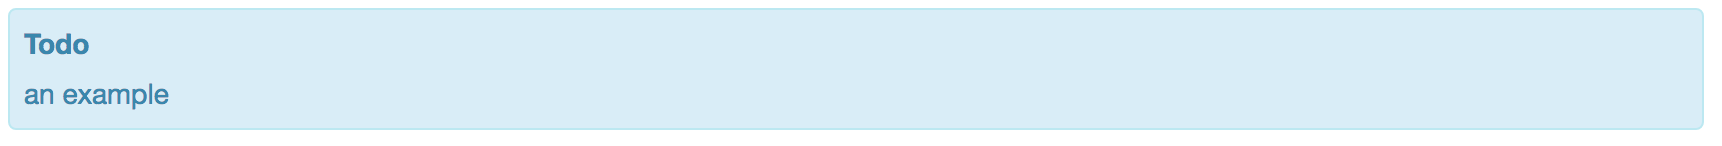
\includegraphics[width=\columnwidth]{../../images/todo.png}

\FILENAME

\section{Markdown}\label{markdown}

The content form this section originates from see:
\url{https://en.wikipedia.org/wiki/Markdown}.

Markdown is a simple markup language, however there is no precise
standard defined for it and implementations may have features not
supported by other implementations. Nevertheless, it provieds as imple
and easy way to quicly develop clean looking documents.

There are severla tools that make markdown attractive allowing to
write the text in one window while at the same time seeing the
rendered out put in another.

This includes

\begin{description}

\item[Macdown] An editor for mardown targeted on OSX

\end{description}

To convert the markdown to other formats with \verb|pandoc|

\begin{verbatim}
# Heading

## Sub-heading

### Another deeper heading
 
Paragraphs are separated
by a blank line.

Two spaces at the end of a line leave a  
line break.

Text attributes _italic_, *italic*, __bold__, **bold**, `monospace`.

Horizontal rule:

---

Bullet list:

  * apples
  * oranges
  * pears

Numbered list:

  1. apples
  2. oranges
  3. pears

A [link](http://example.com).

\end{verbatim}

\subsection{Tools}

\begin{description}
\item [Dilinger] \URL{https://dillinger.io/}. A HTML5 based cloud
  enabled editor. It allows to download the created Markdown.
\item[Macdown] \URL{https://macdown.uranusjr.com/} ``MacDown is an
  open source Markdown editor for macOS''
\end{description}
\FILENAME

\section{Communicating Research in Other Ways}\label{communicating-research}

Naturally, writing papers is not the only way to communicate your
research with others. We find that today we see additional pathways
for cumminication includine blogs, twitter, facebook, e-mail, Web
pages, and electronic notebooks. Let us refisit some of them and
identify when they are helpful.

\subsection{Blogs}\label{blogs}

\begin{description}
\item[blog:]
noun, a regularly updated website or web page, typically one run by an
individual or small group, that is written in an informal or
conversational style.
\end{description}

Advantages:

\begin{itemize}
\tightlist
\item
  encourages spontaneous posts
\item
  encourages small short contributions
\item
  chronologically ordered
\item
  standard software exists to set up blogs
\item
  online services exists to set up blogs
\end{itemize}

Disadvantages:

\begin{itemize}
\tightlist
\item
  structuring data is difficult (some blog software support it)
\item
  not suitable for formal development of a paper
\item
  often lack of sophisticated track change features
\item
  no collaborative editing features
\end{itemize}

\subsection{Sphinx}\label{sphinx}

Sphinx (\url{http://www.sphinx-doc.org/}) is a tool that to create
integrated documentation from a markup language whlie.

Advantages:

\begin{itemize}
\tightlist
\item
  output formats: html, LaTeX, PDF, ePub
\item
  integrates well with directory structure
\item
  powerful markup language (reStructuredText)
\item
  can be hosted on github via github pages
\item
  can integare other renderers such as Markdown
\item
  automatic table of content, tebale of index
\item
  code documentation integration
\item
  search
\item
  written in python and using bash, so extensions and custom automation
  are possible
\end{itemize}

Disadvantage:

\begin{itemize}
\tightlist
\item
  requires compile step
\item
  When using markdown github can render individual page
\end{itemize}

Others:

\begin{itemize}
\tightlist
\item
  Read the Docs (\url{https://readthedocs.org/})
\item
  Doxygen (\url{http://www.stack.nl/~dimitri/doxygen/})
\item
  MkDocs (\url{http://www.mkdocs.org/})
\end{itemize}

\subsection{Notebooks}\label{notebooks}

\subsubsection{Jupyter}\label{jupyter}

The Jupyter Notebook (\url{http://jupyter.org/}) is an open-source web
application allowing users to create and share documents that contain
live code, equations, visualizations and explanatory text. Use cases
include data cleaning and transformation, numerical simulation,
statistical modeling, machine learning.

Advantages:

\begin{itemize}
\tightlist
\item
  Integrates with python
\item
  Recently other programming languages have been integrated
\item
  Allows experimenting with settings
\item
  Allows a form of literate programming while mixing documentation with
  code
\item
  automatically renders on github
\item
  comes with web service that allows hosting
\end{itemize}

Disadvantage:

\begin{itemize}
\tightlist
\item
  mostly encourages short documents
\item
  mark up language is limited
\item
  editing in ASCII is complex and Web editing is prefered
\end{itemize}

\subsubsection{Apache Zeppilin}\label{apache-zeppilin}

A Web-based notebook that enables data-driven, interactive data
analytics and collaborative documents with SQL, Scala and hadoop. It
integrates a web-based notebook with data ingestion, data exploration,
visualization, sharing and collaboration features to Hadoop and Spark.

Advantages:

\begin{itemize}
\tightlist
\item
  integration to various framework
\item
  Web framework
\item
  integration with spark, hadoop
\end{itemize}

Disadvantages:

\begin{itemize}
\tightlist
\item
  larger framework
\item
  must leverages existing deployments of spak, hadoop
\end{itemize}


\begin{comment}
\subsection{References}\label{references}

Collaboratories:

\begin{itemize}
\tightlist
\item
  Myers JD, TC Allison, SJ Bittner, BT Didier, M Frenklach, WH Green, YL
  Ho, J Hewson, WS Koegler, CS Lansing, D Leahy, M Lee, R McCoy, M
  Minkoff, S Nijsure, G von Laszewski, D Montoya, L Oluwole, CM
  Pancerella, R Pinzon, W Pitz, LA Rahn, B Ruscic, KL Schuchardt, EG
  Stephan, A Wagner, TL Windus, and C Yang. 2005. ``A Collaborative
  Informatics Infrastructure for Multi-scale Science.'' Cluster
  Computing 8(4):243-253.
\item
  Metadata in the Collaboratory for Multi-Scale Chemical Science Carmen
  Pancerella, John Hewson, Wendy Koegler, David Leahy, Michael Lee,
  Larry Rahn, Christine Yang, James D. Myers, Brett Didier, Renata
  McCoy, Karen Schuchardt, Eric Stephan, Theresa Windus, Kaizar Amin,
  Sandra Bittner, Carina Lansing, Michael Minkoff, Sandeep Nijsure,
  Gregor von Laszewski, Reinhardt Pinzon, Branko Ruscic, Al Wagner,
  Baoshan Wang, William Pitz, Yen-Ling Ho, David Montoya, Lili Xu,
  Thomas C. Allison, William H. Green, Jr., Michael Frenklach
  \url{http://dcpapers.dublincore.org/pubs/article/view/740/736}
\end{itemize}
\end{comment}



%\part{PI Cluster}

\chapter{TODO: Containers}\label{pi-cluster-form-factor}

\section{Docker Survey}

In 2016 Docker Inc. surveyed over 500 Docker developers and operations
experts in various phases of deploying container-based
technologies. The result is available in the {\em The Docker Survey
  2016}.

\URL{https://www.docker.com/survey-2016}

\begin{figure}[htb]
\centering
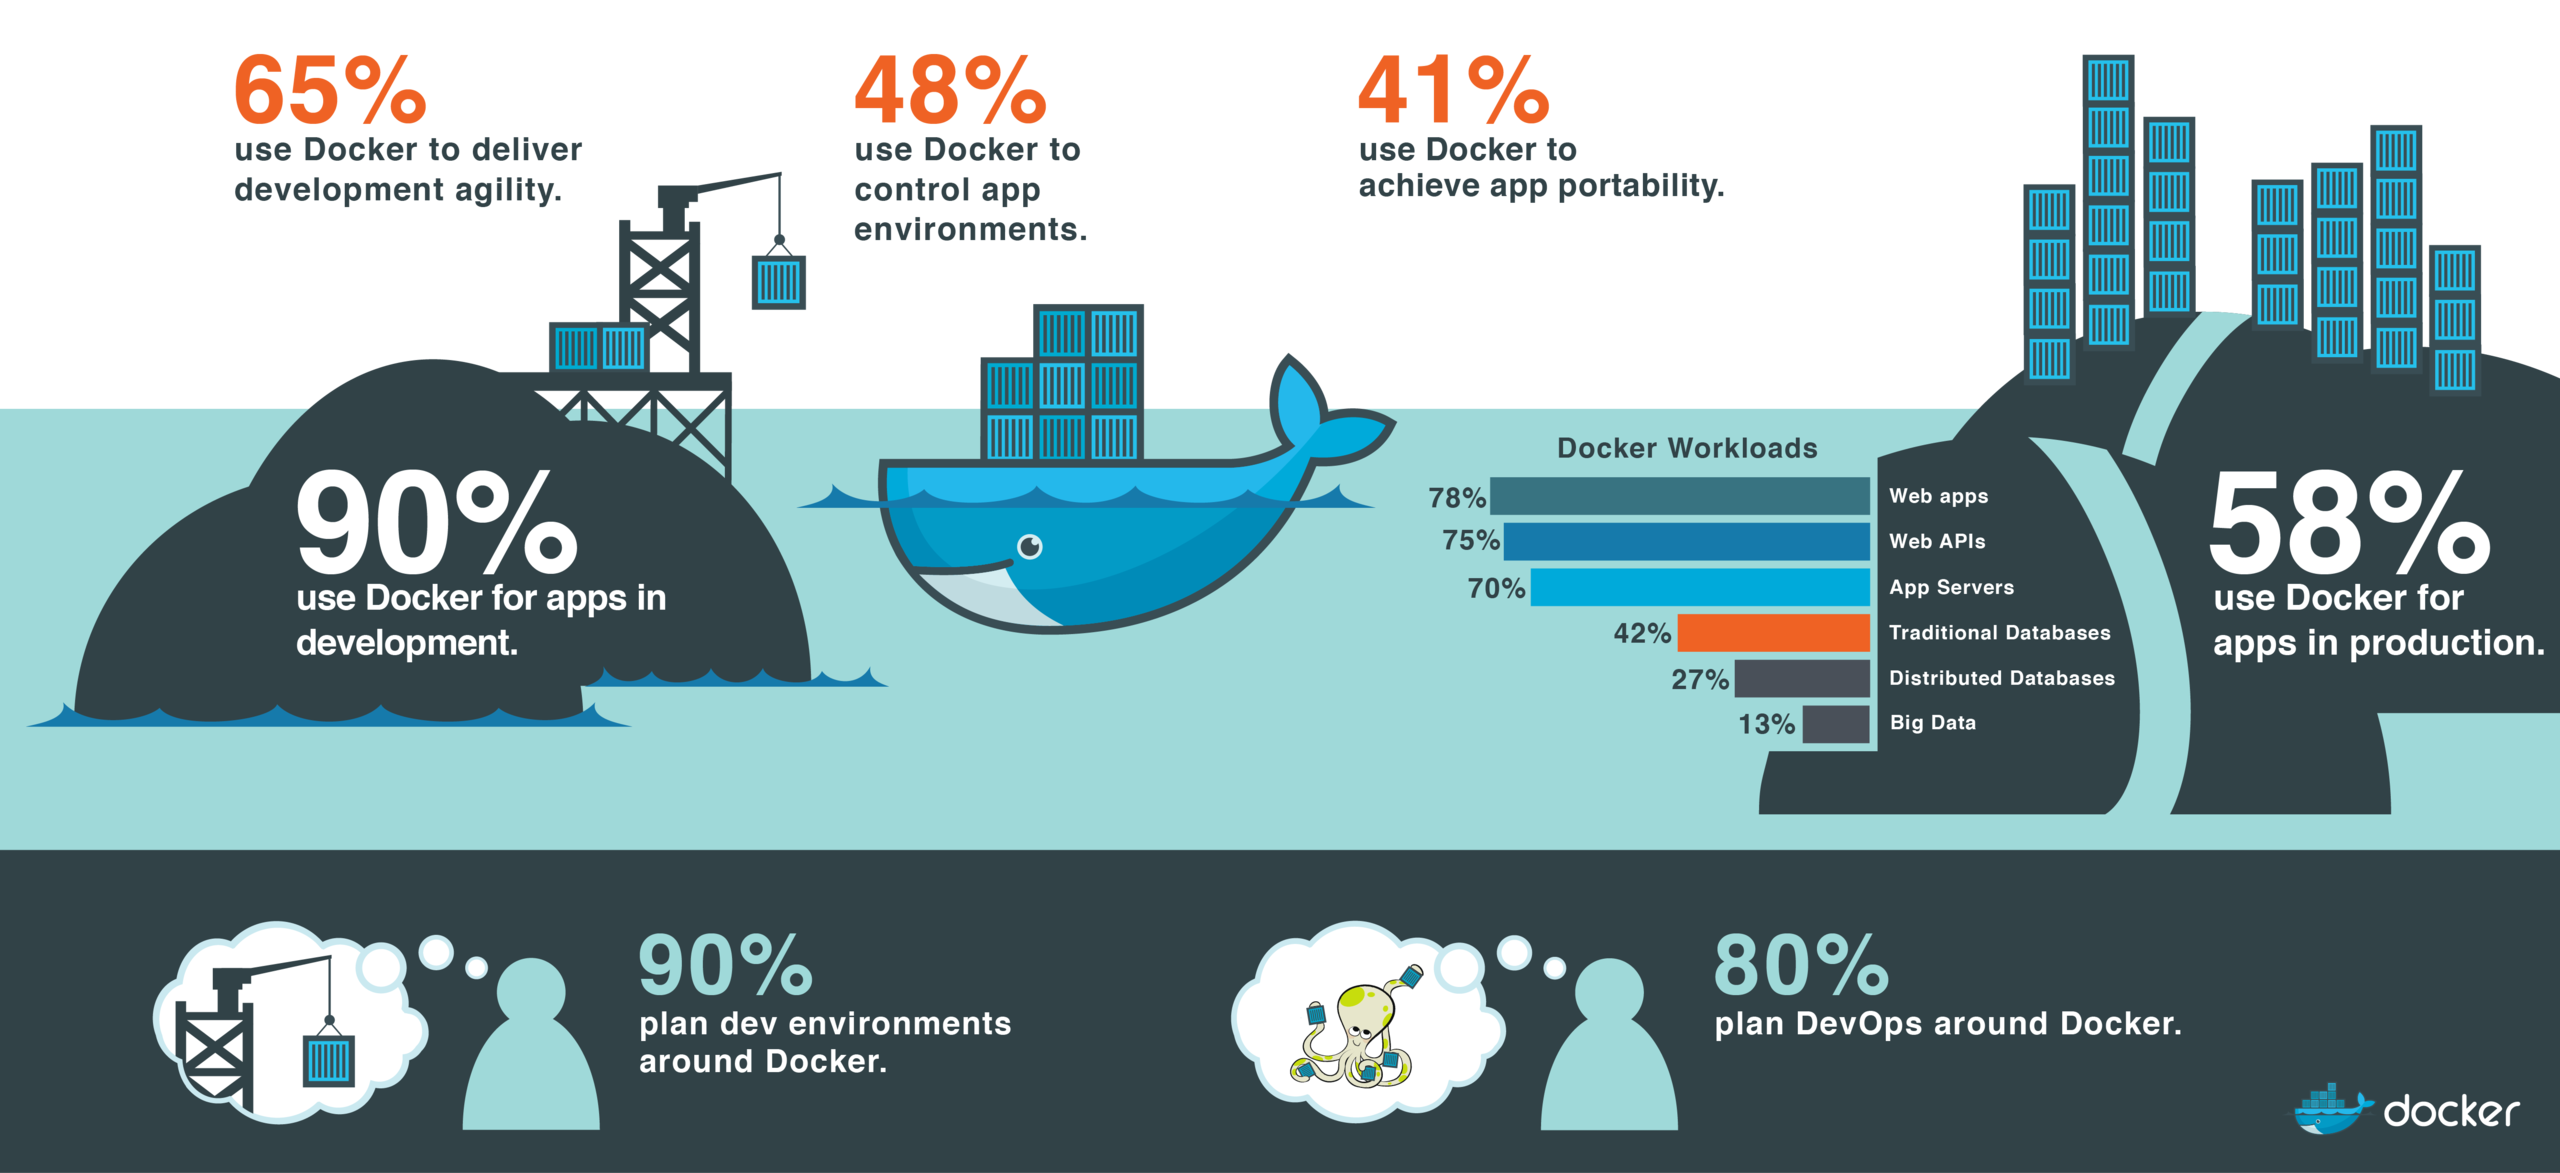
\includegraphics[width=1.0\textwidth]{docker-survey.png}
\caption{Docker Survey Results 2016
}
\end{figure}


\section{Docker Overview}

\URL{https://docs.docker.com/engine/docker-overview/}


\begin{figure}[htb]
\centering
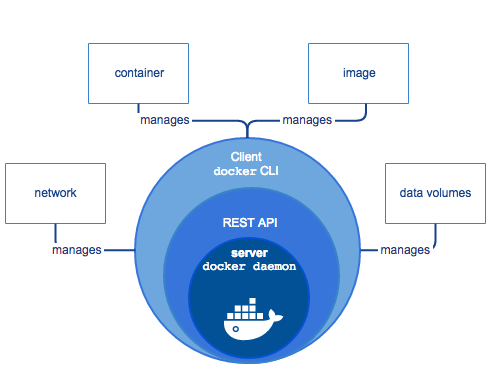
\includegraphics[width=0.5\textwidth]{engine-components-flow.png}
\caption{ Docker Engine Component Flow }
\end{figure}

\begin{figure}[htb]
\centering
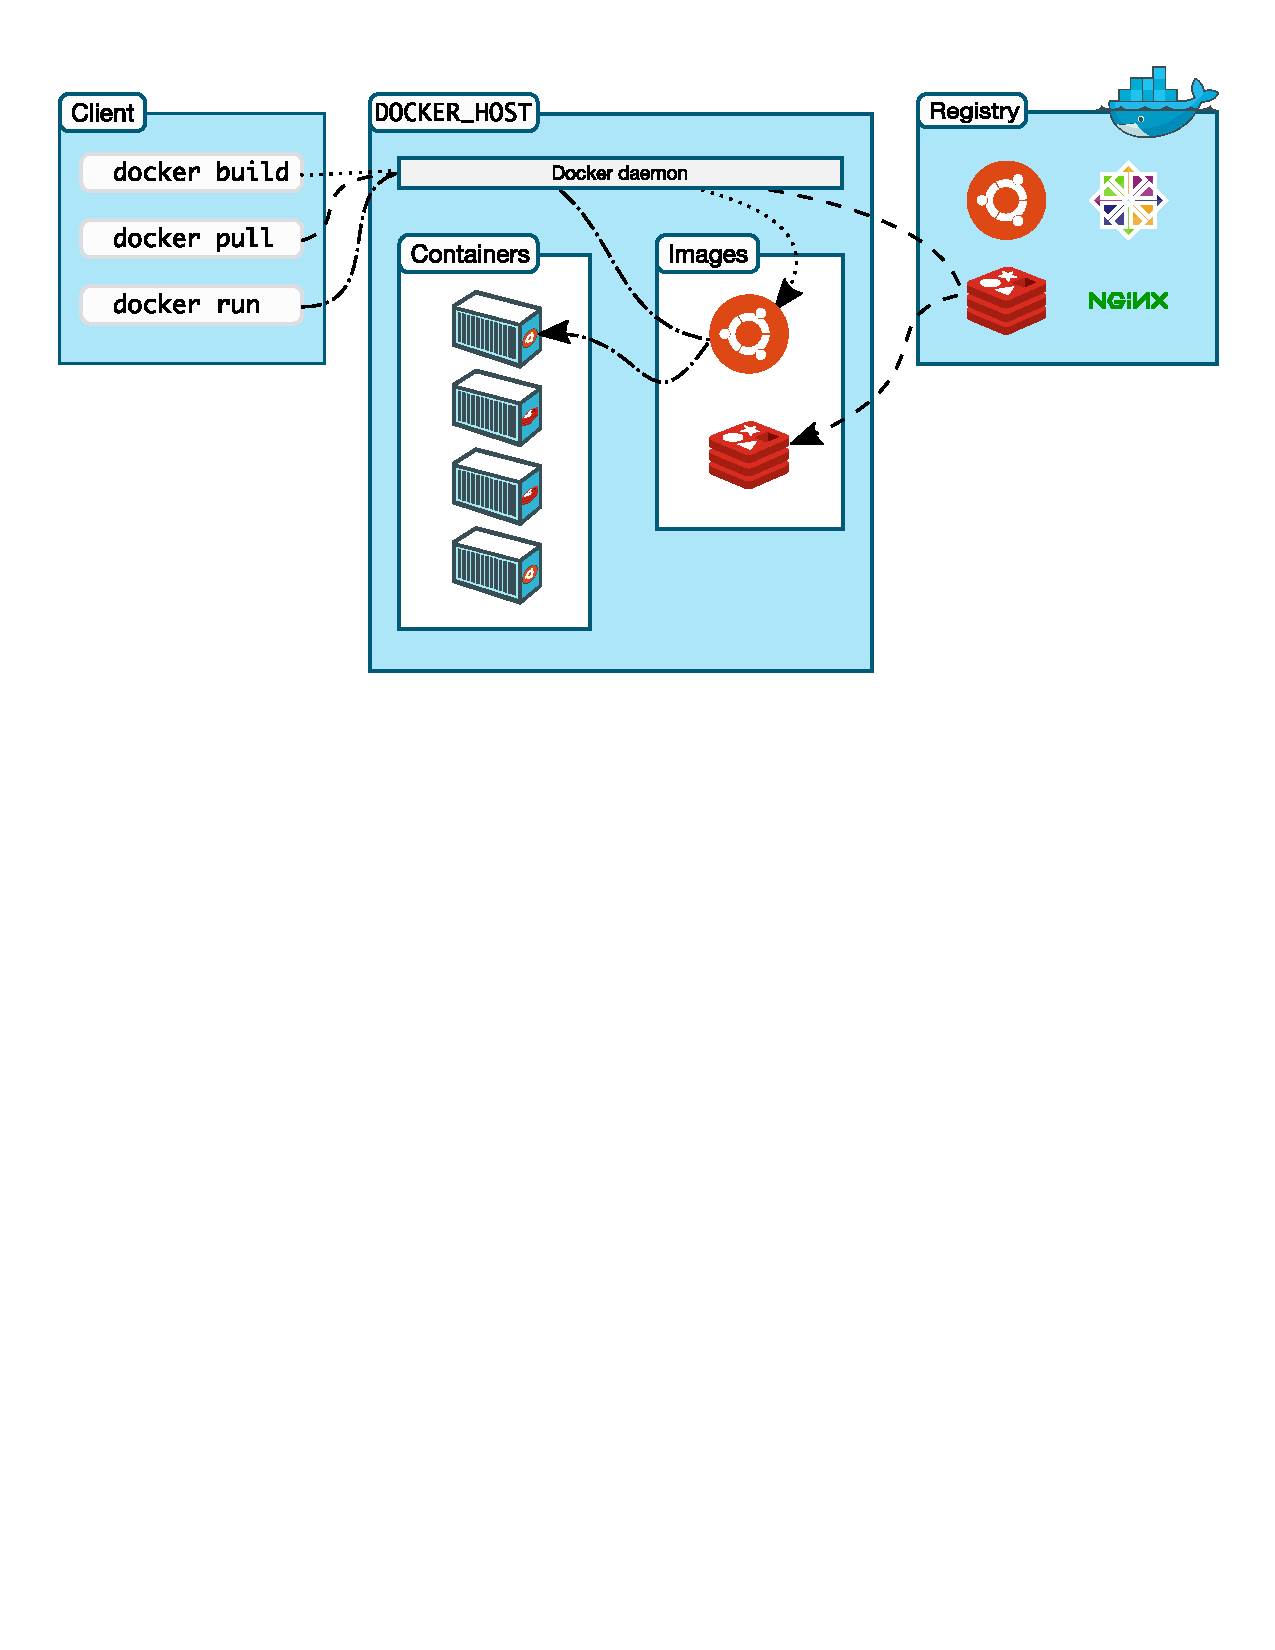
\includegraphics[width=1.0\textwidth]{docker-architecture.pdf}
\caption{ Docker Architecture }
\end{figure}



\section{Container Orchestration Tools: Compare Kubernetes vs Docker Swarm}

\URL{https://platform9.com/blog/compare-kubernetes-vs-docker-swarm/}

\section{Gentle introduction to Containers}

\URL{https://www.slideshare.net/jpetazzo/introduction-docker-linux-containers-lxc}

\section{Tutorialspoint}

\URL{https://www.tutorialspoint.com/docker/index.htm}

\URL{https://www.tutorialspoint.com/docker/docker_tutorial.pdf}

\URL{https://www.tutorialspoint.com/docker/docker_pdf_version.htm}

\section{Tutorial: Docker Swarm on Google Compute Engine}

\URL{https://rominirani.com/docker-swarm-on-google-compute-engine-364765b400ed}

\section{Docker Swarm Tutorial}

https://rominirani.com/docker-swarm-tutorial-b67470cf8872

\section{Spark Cluster}

Scalable Spark Deployment using Kubernetes - Part 8 : Meetup Talk

\URL{http://blog.madhukaraphatak.com/scaling-spark-with-kubernetes-part-1/}
\URL{http://blog.madhukaraphatak.com/scaling-spark-with-kubernetes-part-2/}
\URL{http://blog.madhukaraphatak.com/scaling-spark-with-kubernetes-part-3/}
\URL{http://blog.madhukaraphatak.com/scaling-spark-with-kubernetes-part-4/}
\URL{http://blog.madhukaraphatak.com/scaling-spark-with-kubernetes-part-5/}
\URL{http://blog.madhukaraphatak.com/scaling-spark-with-kubernetes-part-6/}
\URL{http://blog.madhukaraphatak.com/scaling-spark-with-kubernetes-part-7/}
\URL{http://blog.madhukaraphatak.com/scaling-spark-with-kubernetes-part-8/}
\URL{http://blog.madhukaraphatak.com/scaling-spark-with-kubernetes-part-9/}

\chapterimage{pi-cluster.jpg} % Chapter heading image

\chapter{Pi Cluster Form Factor}\label{c:pi-cluster-form-factor}


In this chapter we will discuss a number of opportunities to build
small scale compute and cluster resources using Raspberry Pi's.

This includes the following:

\begin{itemize}

\item a NAS server with one Raspberry Pi 3 (Section~\ref{nas-1-pi})

\item a Cluster using 1 Raspberry Pi as master and 4 Raspberry Zeros
  as workers (Section~\ref{clusterhat-4-zero-1-pi})

\item a Cluster with 5 Raspberry Pi's (Section
 ~\ref{S:cluster-case-with-cooling-5-pi}). A minimum of 3 is needed.

\item a Cluster with 40 Raspberry Pi's (Section
 ~\ref{bitscope-case-40-pi})

\item a Cluster with 144 Raspberry Pi's (Section
 ~\ref{bitscope-cluster-144-pi})

\item our recommended 5 node Raspberry Pi Cluster (Section
 ~\ref{s:pi5}). 3 nodes need to be used at minimum.
 

\end{itemize}

\section{NAS (1 Pi)}\label{nas-1-pi}

Although a NAS is not really a compute cluster the Pi has used many
times to build a Network Attached Storage (NAS) server. In this
configuration a HDD is attached to the Raspberry and the network
features of the Raspberry is used to access the disk drive via
software installed on the PI that make this easily possible. Many
tutorials exists on the Web that help setting op such a device.

We like to hear from you if you have successfully developed such a NAS
and provide us with such links. Links that may help include:

  \URL{https://hackmypi.com/NASpi.php}


\section{ClusterHat (4 Zero + 1 Pi)}\label{clusterhat-4-zero-1-pi}

The smallest cluster we came across is actually a hybrid cluster in
which 4 Pi zeros attached to a Raspberry Pi 3. Thi sis achieved via an
add on board to the Pi 3 allowing to plug in PI=i Zeros:


  \URL{https://clusterhat.com/}


The Cluster HAT (Hardware Attached on Top) allows to attach 4 Raspberry
Pi Zeros via to be attached to a regular Raspberry PI 3 to simulate a
small cluster.

According to the Web Site it supports the following features:



\begin{itemize}
\item
  USB Gadget Mode: Ethernet and Serial Console.
\item
  Onboard 4 port USB 2.0 hub.
\item
  Raspberry Pi Zeros powered via Controller Pi GPIO (USB optional).
\item
  Individual Raspberry Pi Zero power controlled via * Controller Pi GPIO
  (I2C).
\item
  Connector for Controller Serial Console (FTDI Basic).
\item
  Controller Pi can be rebooted without interrupting power to Pi Zeros
  (network recovers on boot).
\end{itemize}

\begin{figure}
\centering
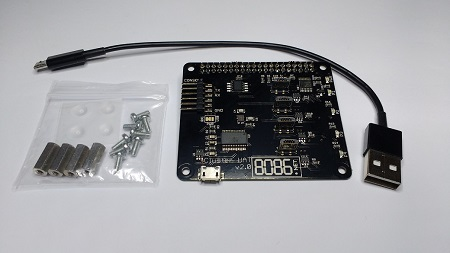
\includegraphics[width=0.5\textwidth]{ClusterHAT-v2-supplied-sm.jpg}
\caption{clusterhat}
\end{figure}



Links:


\URL{https://www.raspberrypi.org/magpi/clusterhat-review-cluster-hat-kit/}{clusterhat
  on raspberrypi.org}


Although this setup seems rather appealing, the issue is with obtaining
Pi Zeros for the regional price of \$5. Typically users can only by one
for that price and must pay shipping. To by more one has to buy a kit
for about \$20. However, for that amount of money it may just be worth
while to get Pi 3's instead of zero's. Nevertheless the formfactor is
rather appealing.

\section{Cluster Case With Cooling (5 Pi)}\label{S:cluster-case-with-cooling-5-pi}

Many instructions on the Web exist describing how to build clusters with
3 or more Pi's. One of the considerations that we have to think about is
that we may run rather demanding applications on such clusters causing
heat issues. To eliminate them we must provide proper cooling. In some
cluster projects cooling is not adequately addressed. Hence we like to
provide an example that discusses in detail how to add a fan and what the
fan has for an impact on the temperature.

\begin{figure}
\centering
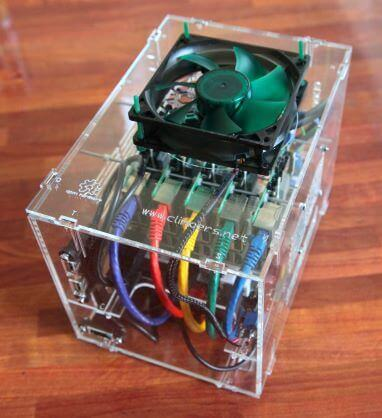
\includegraphics[width=0.5\textwidth]{IMG16_6273_sweb.jpg}
\caption{}
\end{figure}


\URL{http://climbers.net/sbc/add-fan-raspberry-pi/}

\URL{http://climbers.net/sbc/diy-raspberry-pi-3-cluster/}


From the above Web page we find the following information as shown in
Table~\ref{F:pi-fan}. From the data in the table it is clear that we
need to keep the Pi from throttling while being in a case by adding a
fan as obvious from experiment No. 2.



\begin{table}[htb]
\caption{Temperature comparision of fan impact}\label{F:pi-fan}
\bigskip
\begin{center}
\begin{tabular}{llllllll}
\hline
No. & Case & Fan & Direction & RPM & Idle & 100\% Load &
Performance\tabularnewline
\hline
1 & no & no & - & - & 41.0C & 75.5C & OK (barely)\tabularnewline
2 & yes & no & - & - & 45.0C & 82.5C & throttles\tabularnewline
3 & yes & 5V & in & unkown & 37.9C & 74.5C & OK (barely)\tabularnewline
4 & yes & 7V & in & 800 & 35.6C & 69.5C & OK\tabularnewline
5 & yes & 12V & in & 1400 & 32.5C & 61.1C & OK\tabularnewline
6 & yes & 7V & out & 800 & 34.5C & 66.4C & OK\tabularnewline
\hline
\end{tabular}
\end{center}
\end{table}




\section{Bitscope Case (40 Pi)}\label{bitscope-case-40-pi}

A company from Australia called BitScope Designs offers a number of
cases that leverage their Pi Blade boards allowing up to four Pis to be
put together and sharing the same power supply. The blades are shown in
Figure b.1. The rack to place 10 of them is shown in Figure b.2.

\begin{figure}
\centering
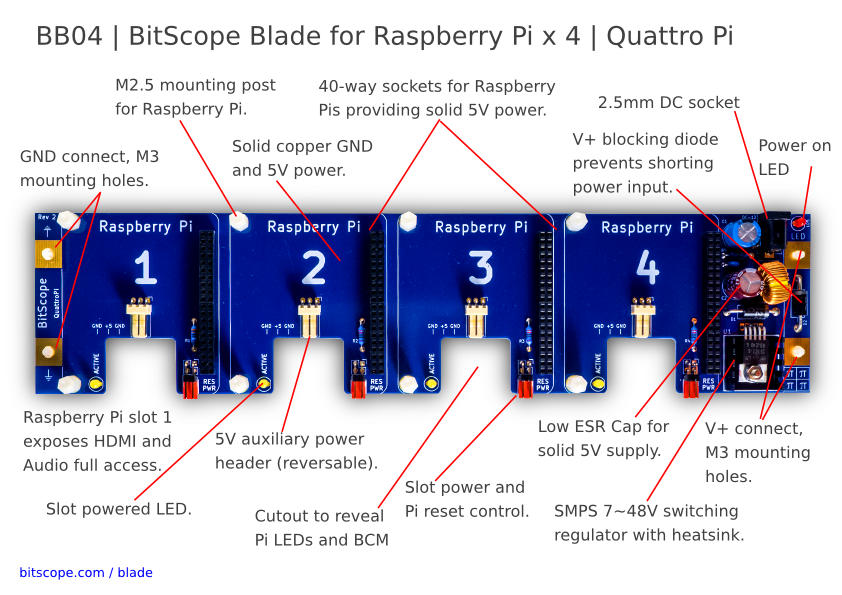
\includegraphics[width=0.3\textwidth]{04.jpg}
\caption{Bitscope blade for 4 Pi's.}
\end{figure}


\begin{figure}
\centering
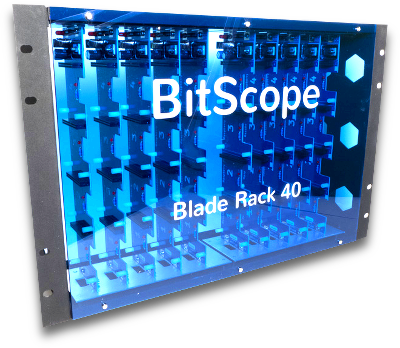
\includegraphics[width=0.3\textwidth]{br40a.png}
\caption{40 Pi Blade rack.}
\end{figure}


The cost of the balde rack is \$ 795.45 + \$60.00 shipping + import tax.
This may originally sound expensive when compared to a single case,
however as we can store 40 Pis in them and they can share the
power-supply and reduce cabeling we think this case is quite interesting
overall due to its price-point of \$20 per Pi.



\section{Bitscope Cluster (144 Pi)}\label{bitscope-cluster-144-pi}

https://www.youtube.com/watch?v=78H-4KqVvrg

Together with LANL a new cluster module that holds 144 Pis is developed.
This sytem is targeted to be placed into a rack to create a large Pi
cluster. The cost for such a module is about \$15K. Figure
\ref{F:pi-mod-1} shows the
module and Figure~\ref{F:pi-mod-2} shows how multiple modules can be placed into a
single rack.

\begin{figure}
\centering
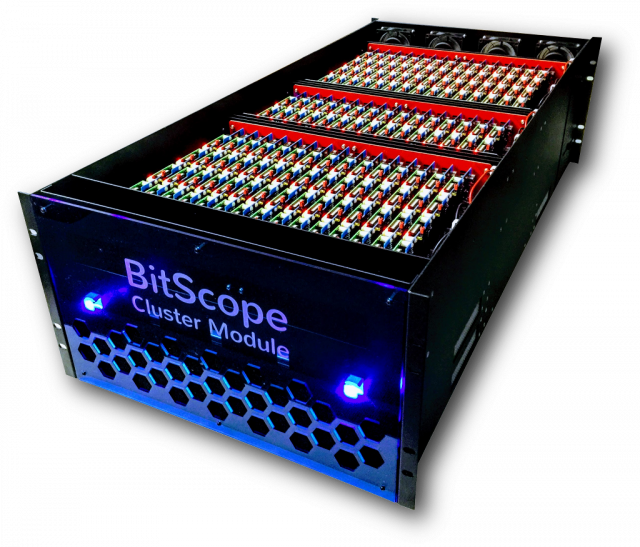
\includegraphics[width=0.5\textwidth]{cluster-module.png}
\caption{Bitscope 144 cluster module.}\label{F:pi-mod-1}
\end{figure}

\begin{figure}
\centering
\includegraphics[width=0.5\textwidth]{rack-overview.png}
\caption{Rack placement of multiple Bitscope 144 cluster modules.}\label{F:pi-mod-2}
\end{figure}




\subsection{Links}\label{links}

Additional information about this form factor can be found at the
following links:

\URL{https://cluster.bitscope.com/solutions}
\URL{https://www.pcper.com/news/General-Tech/BitScope-Unveils-Raspberry-Pi-Cluster-2880-CPU-Cores-LANL-HPC-RD}
\URL{http://my.bitscope.com/store/}
\URL{http://my.bitscope.com/store/?p=view\&i=item+7}
\URL{http://www.newark.com/bitscope/bb04b/quattro-pi-board-raspberry-pi/dp/95Y0643}
\URL{http://linuxgizmos.com/rpi-expansion-boards-support-up-to-40-pi-clusters/}



\section{Build Your Own 5 Node Pi Cluster}\label{s:pi5}

To experiment with building an elementary cluster one does not need to
have a big budget. Such clusters are often dedicated to research tasks
and are bound into security protocols that do not allow direct
access. Instead it is possible to build such a cluster based on
Raspberry PI's yourself if you are willing to spend the money or if
you have access to PI's that you may loan from your department.

Table~\ref{T:picluster-partslist} lists one such possible parts list
that will allow you to build a cluster for up to 5 nodes. However make
sure to buy at least 3 Raspberry PI's with the appropriate memory. At
minimum we recommend you get the 32GB SD card. We do not recommend any
smaller as otherwise you will run out of memory. Additionally, you can
add memory and disks on te USB ports. If you attach a HDD, make sure
it has an external power supply and do not drive it from the USB power
as otherwise the PI becomes unstable.  A fan is at this time not yet
included.

Naturally it is possible to modify the parts list and adapt. If you
find better parts let us know. We have not included any case and you
are welcome to share your suggestions with the class. For a case we
are looking also for a good solution for a fan.

We suggest that when you build the cluster to do it on a table with a
large white paper or board, or a tablecloth and take pictures of the
various stages of the build so we can include it in this document.

Initially we just put rasbian as Operating system on the SD cards and
test out each PI. To do so you will naturally need an SD card writer
that you can hook up to your computer if it does not have one. As you
will have to potentially do this more than once it is not recommended
to buy an SD card with the OS on it. Buy the SD card writer instead so
you can redo the flashing of the card when needed. In addition to the
SD card you need a USB mouse and keyboard and a monitor or TV with
HDMI port.

Locate setup instructions and write  a tutorial in markdown that we
will include here once it is finished. The tutorial is to be managed
on github.

\TODO{Class: check the network hub if it is a good choice as the one we
  originally chose could not be brought in sufficient quantity.}

\begin{table}[htb]

\caption{Parts list for a Pi cluster, remember you need at least 3
  Raspberry Pis}\label{T:picluster-partslist}
\bigskip


\resizebox{\textwidth}{!}{%
\begin{tabular}{rp{13cm}p{1cm}}
  \hline
  Price   &  Description & URL          \\
  \hline
  \hline
  \$29.99 & 
            Anker 60W 6-Port USB Wall Charger, PowerPort 6 for iPhone 7 / 6s /
            Plus, iPad Pro / Air 2 / mini, Galaxy S7 / S6 / Edge /
            Plus, Note 5 / 4, LG, Nexus, HTC and More  
                         & 
                           \href{https://www.amazon.com/Anker-6-Port-Charger-PowerPort-iPhone/dp/B00P933OJC/ref=pd\_sim\_107\_70?\_encoding=UTF8\&psc=1\&refRID=B1S6V5G0CTJ9NH5G0CRT}{link}
  \\

  \$8.90  & 
            Cat 6 Ethernet Cable 1 ft White ( 6 Pack ) – Flat Internet Network
            Cable – Jadaol Cat 6 Computer Cable short - Cat6 Ethernet
            Patch Lan Cable With &
                                   \href{https://www.amazon.com/Cat-Ethernet-Cable-White-Pack/dp/B01IQWGI0O/ref=sr\_1\_1?s=electronics\&ie=UTF8\&qid=1513699717\&sr=1-1\&keywords=Cat+6+Ethernet+Cable+1+ft+White+\%28+6+Pack+\%29+\%E2\%80\%93+Flat+Internet+Network+Cable+\%E2\%80\%93+Jadaol+Cat+6+Computer+Cable+short+-+Cat6+Ethernet+Patch+Lan+Cable+With\%E2\%80\%A6}{link}  \\

  $^{(1)}$ \$19.99 &  D-link 8-Port Unmanaged Gigabit Switch
            (GO-SW-8G)   & 
                           \href{https://www.amazon.com/D-link-8-Port-Unmanaged-Gigabit-GO-SW-8G/dp/B008PC1MSO}{link}      \\


  \$10.49 &  SanDisk Ultra 32GB microSDHC UHS-I Card with
            Adapter, Grey/Red, Standard Packaging
            (SDSQUNC-032G-GN6MA)
                         & 
                           \href{https://www.amazon.com/SanDisk-microSDHC-Standard-Packaging-SDSQUNC-032G-GN6MA/dp/B010Q57T02/ref=sr\_1\_10?s=pc\&rps=1\&ie=UTF8\&qid=1498443283\&sr=1-10\&refinements=p\_85:2470955011,p\_n\_feature\_two\_browse-bin:6518304011,p\_n\_feature\_keywords\_two\_browse-bin:5947557011}{link}       \\

  \$8.59  & Short USB Cable, OKRAY 10 Pack Colorful Micro
            USB 2.0 Charging Data Sync Cable Cord for
            Samsung, Android Phone and Tablet, Nexus, HTC,
            Nokia, LG, Sony, Many Digital Cameras-0.66ft
            (7.87 Inch) & 
                          \href{https://www.amazon.com/OKRAY-Colorful-Charging-Samsung-Cameras-0-66ft/dp/B00R5GZJR6/ref=sr\_1\_6?s=pc\&ie=UTF8\&qid=1498447476\&sr=1-6\&keywords=micro+usb+cable+1ft}{link}         \\


  \$7.69    & 50 Pcs M2 x 20mm + 5mm Hex Hexagonal Threaded
              Spacer Support
                         & 
                           \href{https://www.amazon.com/20mm-Hexagonal-Threaded-Spacer-Support/dp/B00FH8AB8Q/ref=sr\_1\_9?s=industrial\&ie=UTF8\&qid=1513700337\&sr=1-9\&keywords=hex+spacers+m2+20mm}{link}
  \\

  \$7.99  & Easycargo 15 pcs Raspberry Pi Heatsink Aluminum
            + Copper + 3M 8810 thermal conductive adhesive
            tape for cooling cooler Raspberry Pi 3, Pi 2,
            Pi Model B+
                         & 
                           \href{https://www.amazon.com/Easycargo-Raspberry-Heatsink-Aluminum-conductive/dp/B07217N5LS/ref=sr\_1\_3?s=industrial\&ie=UTF8\&qid=1513700498\&sr=1-3\&keywords=raspberry+pi+3}{link}
  \\

  \$34.49 & Raspberry Pi 3 Model B Motherboard  (you need at least 3 of them)   & 
                                                                                  \href{https://www.amazon.com/Raspberry-Pi-RASPBERRYPI3-MODB-1GB-Model-Motherboard/dp/B01CD5VC92}{link}
  \\

 $^{(2)}$ \$59.99 & 1TB drive   & \href{http://wdlabs.wd.com/products/wd-pidrive-berryboot-edition/}{link}    \\

  \$15.19 & 64GB flash  & \href{https://www.wdc.com/products/wdlabs/wd-pidrive-foundation-edition.html\#WD3750LMCW}{link} \\

  \$6.99  & HDMI Cable, Rankie 2-Pack 6FT Latest Standard
            HDMI 2.0 HDTV Cable - Supports Ethernet, 3D, 4K
            and Audio Return (Black) - R1108
                         & 
                           \href{https://www.amazon.com/Cable-Rankie-2-Pack-Latest-Standard/dp/B00Z07XQ4A/ref=sr\_1\_6?s=wireless\&ie=UTF8\&qid=1513782649\&sr=1-6\&keywords=hdmi+cable+6ft}{link}         \\

  \$12.99  & AUKEY USB C Adapter, USB C to USB 3.0 Adapter
             Aluminum 2 Pack for Samsung Note 8 S8 S8+,
             Google Pixel 2 XL, MacBook Pro, Nexus 6P 5X, LG
             G5 V20 (Gray)
                         & 
                           \href{https://www.amazon.com/Cat-Ethernet-Cable-White-Pack/dp/B01IQWGI0O/ref=pd\_sim\_147\_2?\_encoding=UTF8\&psc=1\&refRID=FZZ7E36666EJPDTH7B6A}{link}     \\

\$19.19 & For Raspberry Pi 3 2 TFT LCD Display, kuman 3.5
   Inch 480x320 TFT Touch Screen Monitor for
   Raspberry Pi Model B B+ A+ A Module SPI
   Interface with Touch Pen SC06
     & 
\href{https://www.amazon.com/Raspberry-Display-kuman-480x320-Interface/dp/B01CNJVG8K/ref=sr\_1\_1?s=electronics\&ie=UTF8\&qid=1513783748\&sr=1-1\&keywords=pi+3+lcd+screen+3.5in}{link} \\
\hline
\end{tabular}
}
\smallskip

{\footnotesize (1) items were replaced with similar item}\\
{\footnotesize (2) item was not available}

\end{table}


\begin{exercise}
\label{E:cluster-pi}
In case you do not have access to multiple PIs conduct the Single Pi
experiment.
\end{exercise}

\section{Single Pi}


You have been presented in Section
\ref{S:cluster-case-with-cooling-5-pi} with a table that compares
tempreatures. Your task is to identify issues with the experiment and
the table.  Furthermore we like you to rerun a temperature experiment
in the entire class.

\TODO{Gregor: Add IoT section and PI configuration}

\begin{enumerate}
\item
  Get a PI3 modeL B, an HDMI cable, a power supply, a case. Such a
  configuration is listed in the IoT section. 
\item
  Buy or manufacture a case of your choice. You can use a 3d-printer
  if you have one available.
\item
  Conduct a temperature experiment.
\end{enumerate}

Discussion of these assignment is to be executed openly in
class. Points will be issued only once the class agrees upon an
experiment.

This exercise is not only to learn about the behaviour of the Pi, but
also about how to coordinate experiments with a large number of
students.


\begin{exercise}
  \label{E:Exercise.Pi.Single.1} What temperature measurement is
  missing from the table.
\end{exercise}

\begin{exercise}
\label{E:.Pi.Single.2} How would you create an experiment under \textit{load}.
\end{exercise}

\begin{exercise}
\label{E:.Pi.Single.3} How would you create an experiment to which all
  students in different classes could contribute their values? Can the
  cloud be used?
\end{exercise}

\begin{exercise}
\label{E:.Pi.Single.4} Collect the information from all class members
  using cloud services.
\end{exercise}

\begin{exercise}
  \label{E:.Pi.Single.5} Identify how to use the VPN server so you can
  use your Laptop instead of a TV or computer monitor. Write a
  tutorial.
\end{exercise}



\section{Small Pi Cluster}

In this set of exercises we will be building a small Raspberry Pi
cluster. All of you will have to do Exercise
\ref{Exercise.Pi.Cluster.Build}, as well as one of the tasks related
to Swarm, kubernetes or Spark.

It is important that you write down all steps very carefully as you
are expected to use the steps to develop an automated deployment. For
your cluster. Your tutorial will be tested by other groups and easy of
installation completness, and correctness will be evaluated.  Teams
that find issues and improve deployment tutorials will receive points.
TA's will also replicate these steps to identify a fair evaluation
without bias.


\begin{exercise}

\label{E:.Pi.Cluster.Build} Build groups of up to 5 people. Make a
  plan on what needs to be done to build the cluster and develop a
  schedule. Include in this plan (a) obtaining the material the
  hardware build, (b) the installation of the operating system (c) the
  testing of the system (d) familiarizing with the OS.
\end{exercise}

\begin{exercise}

  \label{E:.Pi.Cluster.DockerSwarm} Install a docker Swarm cluster on
  your PI. Develop a tutorial in markdown and mind
  plagiarism. Contribute your tutorial to this document to get
  acknowledged and credit. Work with others in class to coordinate a
  single tutorial.
\end{exercise}

\begin{exercise}

  \label{E:.Pi.Cluster.Kubernetes} Install a kubernetes cluster on
  your PI. Develop a tutorial in markdown and mind
  plagiarism. Contribute your tutorial to this document to get
  acknowledged and credit. Work with others in class to coordinate a
  single tutorial.
\end{exercise}
  
\begin{exercise}
  \label{E:.Pi.Cluster.Spark} Install a spark cluster on your
  PI. Develop a tutorial in markdown and mind plagiarism. Contribute
  your tutorial to this document to get acknowledged and credit. Work
  with others in class to coordinate a single tutorial.
\end{exercise}


\subsection{Virtual Raspberry Cluster}

It should also be possible to craete a virtual raspberry PI cluster
while for example using virtual box. This requires two steps. First
the deployment of a virtualized Raspberry PI. The following
information may be useful for this

\URL{http://dbakevlar.com/2015/08/emulating-a-raspberry-pi-on-virtualbox/}

The next step includes the deployment of multiple VMs emulating
Raspberrys. Naturally each should have its own name so you can
distinguish them. INstead of just using the GUI, it would be improtant
to find out how to start them from a commandline as a shell script as
well as tear them down.

Next you will need to make sure you can communicate from the PIs to
each other. This is naturally the same as on a real cluster

\begin{exercise}
provide a tutorial 
\end{exercise}

This can be chosen as part of your project, but you need to develop a
cloudmesh command for managing the cluster. THis includes starting and
stoping as well as checkpointing the cluster from a cloudmesh
command. Furthermore you need to benchmark it and identify how to do
this and contrast this to other clusters that you may start or have
access to. Please get in contact with Gregor. THis prject is reserverd
for online students, as residential students will have access to real
Rasperry PI hardware.



%\FILENAME

\section{Plagiarism}\label{S:plagiarism}

We start with the review of a most important topic.

\subsection{Plagiarism Definition}

In academic life it is important to understand and avoid plagiarism.
The dictionary defines plagiarism as follows \url{dictionary.com}:

% \textipa{['pl\=aj@""riz@m]}

\begin{description}
\item[pla·gia·rism] ``the practice of taking someone else's work or ideas and passing them
off as one's own.''
\end{description}



\subsection{Plagiarism Policies}
Organizations and universities will have policies in place do address
plagiarism. An example is provided for Indiana University
\cite{www-iu-plagiarism}. We quote:

\begin{quotation}
``Honesty requires that any ideas or materials taken from
another source for either written or oral use must be fully
acknowledged. Offering the work of someone else as one’s own is
plagiarism. The language or ideas thus taken from another may range
from isolated formulas, sentences, or paragraphs to entire articles
copied from books, periodicals, speeches, or the writings of other
students. The offering of materials assembled or collected by others
in the form of projects or collections without acknowledgment also is
considered plagiarism. Any student who fails to give credit for ideas
or materials taken from another source is guilty of plagiarism. 

(Faculty Council, May 2, 1961; University Faculty Council, March 11,
1975; Board of Trustees, July 11, 1975)''
\end{quotation}

Faculty members at Universitys are also bound by policies that mandate
reporting. At Indiana University the following policy applies (for a
complete policy see the Web page):

\begin{quotation}
``Should
the faculty member detect signs of plagiarism or cheating, it is his
or her most serious obligation to investigate these thoroughly, to
take appropriate action with respect to the grades of students, and
\textit{in any event} to report the matter to the Dean for Student Services [or
equivalent administrator]. The necessity to report every case of
cheating, whether or not further action is desirable, arises
particularly because of the possibility that this is not the student’s
first offense, or that other offenses may follow it. Equity also
demands that a uniform reporting practice be enforced; otherwise, some
students will be penalized while others guilty of the same actions
will go free.

(Faculty Council, May 2, 1961)''
\end{quotation}

Naturally if a student has any questions about understanding
plagiarism the University can provide assistance. If a student is in
doubt and asks for help this is not considered at that time
plagiarism. 

As you can see from the previous policies, the faculty do not have any
choice but reporting real cases of plagiarism to the university
administration.  Thus you must not hold them personally responsible as
this is part of the tasks they are required to do if they like it or
not. Instead, it is {\bf the responsibility of the authors of the
  document} to assure no plagiarism occurs. If you are a student of a
class that writes a paper or project report this naturally also all
applies to you. In addition, if you work in a team you need to assure
the entire team addresses plagiarism appropriately.

In practice this means that the teachers of a course expect yo know
plagiarism and you need to be informed about it. This is typically
done in other courses. However, as it is often overlooked by the
student we are pointing it out here so we can make sure you contribute
to courses that require you to write papers and reports. This also
means you can not claim you did not know what plagiarism is. You are
required to know what it is, know how to detect it and know how to
avoid it. The resources provided next will give you the necessary
tools and background.

\subsection{Plagiarism Resources}

The \href{http://education.indiana.edu/}{School of Education at Indiana
University} has a significant set of resources to get educated about
plagiarism. These resources are intended to ``preparing educators,
advancing knowledge, and improving education'' \cite{}
\url{https://www.indiana.edu/~istd/patterns.html}

The content here is copied from the Web Page

  \URL{https://www.indiana.edu/~istd/patterns.html}

As such we have not included quotes but refer to their Web page for the
original source which may also include updates. Naturally we do not want
to be accused of plagiarize in a chapter about plagiarism.  Thus assume
the content for the rest ov this chapter are copied from that Web page.

\subsection{Pattern}\label{pattern}

\begin{itemize}
\item
  \href{https://www.indiana.edu/~istd/definition.html}{IU Definition} of
  Plagiarism from Student Code of Conduct
\item
  \href{https://www.indiana.edu/~istd/overview.html}{Overview} How to
  give proper credit, steps.
\item
  \href{https://www.indiana.edu/~istd/cases.html}{Cases} of Plagiarism
  in the US, in the news, and elsewhere
\item
  \href{https://www.indiana.edu/~istd/examples.html}{Examples} Word for
  word, paraphrasing
\item
  \href{https://www.indiana.edu/~istd/practice.html}{Practice} with
  feedback on word-for-word and paraphrasing plagiarism
\item
  \href{https://www.indiana.edu/~istd/test.html}{Test} 10 questions on
  recognizing plagiarism
\item
  \href{https://www.indiana.edu/~istd/sitemap.html}{Tutorial Site Map}
  Expanded table of contents
\item
  \href{https://www.indiana.edu/~istd/resources.html}{Resources}
  Websites, books, dictionary links, references for learning more about
  plagiarism
\end{itemize}

\subsection{Tutorials}\label{S:ptutorial}

A number of tutorials are offerd by Indiana University \href{http://education.indiana.edu/graduate/programs/instructional-systems/index.html}{Instructional
  Systems Technology Department}
 Web pages ealing with plagiarism. Thes include:

\begin{itemize}
\item
  \href{https://www.indiana.edu/~academy/firstPrinciples/choice.html}{Plagiarsim
    Tutorial}
\item
  \href{https://www.indiana.edu/~tedfrick/plagiarism/}{Understanding
  Plagiarism}
\end{itemize}

\subsection{How to Recognize Plagiarism}

We are listing fifteen patterns of plagiarism that are defined on the Web
pages itedntified in Section~\ref{S:ptutorial}:

\begin{tabular}{p{4cm}p{3cm}p{8cm}}
Name & Plagiarism Type & Reason \\
\hline
  \href{patternCluelessQuote.html}{Clueless Quote} &  word-for-word & no
  quotes, no citation, no reference 
\\
  \href{patternCraftyCoverUp.html}{Crafty Cover-up} &  proper paraphrase
  but word-for-word  &  also present
\\
  \href{patternCunningCoverUp.html}{Cunning Cover-up} &  paraphrasing & no
  citation, no reference
\\
  \href{patternDeceptiveDupe.html}{Deceptive Dupe} &  word-for-word  &  no
  quotes, no citation, but has reference
\\
  \href{patternDisconnectedDupe.html}{Delinked Dupe} &  word-for-word  &  no
  reference, even though quotes and citation
\\
  \href{patternDeviousDupe.html}{Devious Dupe} &  correct quote but word-for-word  & 
  also present
\\
  \href{patternDippyDupe.html}{Dippy Dupe} &  word-for-word  &  quotes
  missing, even though full citation and reference
\\
  \href{patternDisguisedDupe.html}{Disguised Dupe} &  looks like proper
  para, but actually word-for-word  &  no quotes, no locator
\\
  \href{patternDoubleTrouble.html}{Double Trouble} & word-for-word  and
  paraphrasing  & although has reference
\\
  \href{patternLostLoser.html}{Linkless Loser} &  word-for-word  &  citation
  and reference lacking, although has quotes and locator
\\
  \href{patternLostLocator.html}{Lost Locator} &  word-for-word  &  missing
  locator, although has quotes, citation, and reference
\\
  \href{patternPointlessParaphrase.html}{Placeless Paraphrase} &  paraphrasing  & 
  no reference, although citation present
\\
  \href{patternSeveredCite.html}{Severed Cite} &  paraphrasing  &  reference
  but no citation
\\
  \href{patternShirkingCite.html}{Shirking Cite} &  word-for-word  &  lacks
  locator and reference, although quotes and citation present
\\
  \href{patternTripleD.html}{Triple D--Disguised Disconnected Dupe} & 
  word-for-word  & looks like proper para, but no quotes, no reference, no locator
\end{tabular}

In addition they do specify  three patterns of
non-plagiarism:

\begin{tabular}{p{2cm}p{4cm}p{8cm}}
Name & Type & Description \\
\hline
\\
  \href{patternCorrectQuote.html}{Correct Quote} &  non-plagiarizm & takes another's words
  verbatim and acknowledges with quotation marks, full in-text citation
  with locator, and reference
\\
  \href{patternProperParaphrase.html}{Proper Paraphrase} &  non-plagiarizm & summarizes
  another's words and acknowledges with in-text citation and reference
\\
  \href{patternMindlessParaphrase.html}{Parroted Paraphrase} &  non-plagiarizm & appears to
  be paraphrasing, and technically may not be plagiarism, but \ldots{}
  ???
\end{tabular}

%

\chapter{Sentient Architecture}

\FILENAME

\begin{figure}
\centering
\includegraphics[width=\columnwidth]{images/sentient.jpeg}
\caption{Sentinent Architecture: Source: \url{https://nicolatriscott.files.wordpress.com/2016/03/caaqt-euyam-jpm.jpg}} 
\end{figure}

\section{Introduction}

What is it

\section{Existing Deployments}

list	existing deployments

\section{Impact}

why is it important

not only science, 

\section{Integration into Cloud Computing and Big Data}

how dos it for to cloud computing and big data (Gregor can do that)


\section{Development}
S Architecture in practice


\subsection{Snowwhite and the Seven$^{+1}$ Dwarfs}

The ISE department at Indiana University has obtained eight dendrites
that were assambled by a number of students so they can be used in
class and in research projects. These dendrites can be accessed in
Smith Research Center and allow students and faculty members to
experiment with them. They are bare dendrites and have no
electronics on them. Hence, you will need a hardware device to
interact with.

The reason we named them \textit{Snowwhite and the Seven$^{+1}$ Dwarfs}
is based on the fact that the dendrites are white, and they need to be
interact with  somone. Beacuse of the white color we name the controll
unit snowwhite. The dendrites that are interacting with it are called
dwarfs as this just fits to the name snowwhite. As we actually have 8
and not 7 we added $^{+1}$.


We do not recommend to directly attach the
wires to boards, as they will draw too much power and destroy the
boards. Instead you will need a relay that you controll that itself
controlls the dendrite These can be:

\begin{description}

\item[Arduino:] These boards very simple but provide relative good
  protection of the output links. The disadvantage is that its
  interface is in C.

\item[Teensy] Whatever is now on it TBD

\item[Raspberry Pi] We recommend to use a Raspberry Pi as it has a
  great operating system and is more suited for additional analysis of
  data within an Edge Computing network than the other two choices. It
  also allows you to use python which is clearly a pluss as most of
  the material presented here are in Python.

\end{description}


\begin{figure}
\centering
\includegraphics[width=\columnwidth]{images/snowwhite.jpg}
\caption{Snowwhite and the Seven$^{+1}$  Dwarfs}
\label{F:snowwhite}
\end{figure}


\subsection{Liddy Hall Installation}

architecture drawing


\section{Sentinent Cloudmesh}

	Gregor provides introduction to cloudmesh (probably just pointer to other section)

	Gregor provides introduction to cloudmesh.pi 

	Introduction to parallel programming in python (TBD)

	Towards the Cloudmesh Parallel S development environment


\paragraph{Snowwhite and the Seven$^{+1}$ Dwarfs}

Test environment (8 dendrites)

\paragraph{Liddy Hall}

Andreas dsecribes how we program them 

(Andreas provides)


than we use cloudmesh to interface with them, maybe we need to just
show how we integrate them into mqtt (this is snowhwite) and than we  
can progrem them from another pi

	Test environment Liddy hall 

\section{Alternative Boards}

\subsection{Mega 2560}

``The MEGA 2560 is designed for more complex projects. With 54 digital
I/O pins, 16 analog inputs and a larger space for your sketch it is
the recommended board for 3D printers and robotics projects. This
gives your projects plenty of room and opportunities.'' 
\url{https://store.arduino.cc/usa/arduino-mega-2560-rev3}
A nice case such as the one offered at Amazon will provide good
protection \url{https://www.amazon.com/Eleduino-Arduino-Mega-2560-Enclosure/dp/B016QE46RQ}


\begin{figure}
\centering
\includegraphics[width=0.25\columnwidth]{images/mega2560.jpg}
\caption{MEGA 2560}
\label{F:mega2560}
\end{figure}


\subsection{Programming with Teensy}

``The Teensy is a complete USB-based microcontroller development
system, in a very small footprint, capable of implementing many types
of projects. All programming is done via the USB port.'' Source: \url{https://www.pjrc.com/teensy/}

Current state of programming (whateverthey have)

Which version



\section{Exercises}

\begin{description}

\item[Sentinent.1] Build dendrite. In this excersise you will be
  building a dendrite that you can add to the available pool of dendrites.
\item[Sentinent.2.1] Develop cloudmesh sensor/actuary. In this excersise
  you will be developing an actuator ar sensor interface in object
  oriented programming methodology. You can see many examples in
  cloudmesh.py on github,com. You will pick a sensor you have access
  to and that is not already included in cloudmesh.pi. 
\item[Sentinent.2.2] If you do
  prefer using another board, the option may exist do develp an
  interface for the sensor or actuator for this device. If OO
  programming is not available for that board, a clean design based on
  functions must be provided. However we believe this is mor complex
  than using the Pi. 
\item[Sentinent.3.1] Develop an mqtt based event publisher and
  subscription service. Use first LEDs to test your service before you
  hook up relays and dendrites.
\item[Sentinent.3.2] Hook up the dendrites to mqtt and controll them
\item[Sentinent.4] Develop sensors that interact with the dendrites
\item[Sentient.5] Explore the Page at
  \url{https://www.intorobotics.com/alternative-arduino-boards/} that
  lists a number of PI/Arduino alteranative boards provide a non
  plagiarized table for this chapter and evaluate which could be
  viable alternatives. If you have one of them we like you to provide
  a documentation on how to integrate them with the dendrites.

\end{description}

 


%%----------------------------------------------------------------------------------------
%	PART
%----------------------------------------------------------------------------------------

\part{Developmet Tools}

\FILENAME

\section{Git}\label{git}

This class uses open source technology and we like that you benefit from
material others in the class are developing or have developed. All
assignments are openly submitted to the class github for everyone to
see. As part of the goal of this class is to develop reusable
instructions, deployments, software, and examples. Such reuse is only
possible if the code is publicly available and others can benefit from
it. While using github.com we make sharing of information possible so
every one can benefit and achieve their best.

\subsection{Install}\label{install}

Information on how to install git can be found at

\URL{https://www.atlassian.com/git/tutorials/install-git}

\subsubsection{Config}\label{config}

Once you've got Git installed, several bits of configuration will
enhance your experience with the tool and better tune it to your
operating system. Let us tell you about settings for your username and
email address, line endings, and color, along with the settings'
associated configuration scopes.

\URL{https://www.youtube.com/watch?v=ZChtKFLiaNw}

It is important is that you always want to make sure that you want to
use the git config command to initialize git for the first time you use
it. This will ensure that you use on all resources the same Name and
e-mail so that git history and log will show consistently your checkins.
If you do not do this, your checkins in git do not show up in a
consistent fashion as a single user. This is done with the following
commands:

\begin{verbatim}
$ git config --global user.name "Albert Zweistein"
$ git config --global user.email albert.zweistein@gmail.com
\end{verbatim}

You can set also the editor with:

\begin{verbatim}
$ git config --global core.editor emacs
\end{verbatim}

You will also need to decide if you want to push branches individually
or all branches at the same time. It will be up to you to make what
whill work for you best. We found that the following seems to work best:

\begin{verbatim}
git config --global push.default matching
\end{verbatim}

More information about a first time setup is documented at:

\begin{verbatim}
* http://git-scm.com/book/en/Getting-Started-First-Time-Git-Setup
\end{verbatim}

To check your setup you can say:

\begin{verbatim}
$ git config --list
\end{verbatim}

In addition the tutorials from atlasian are a good source. However
remember that you may not use bitbucket as the repository, so ignore
those tutorials. We found the following useful

\begin{itemize}
\tightlist
\item
  What is git: \url{https://www.atlassian.com/git/tutorials/what-is-git}
\item
  Installing git:
  \url{https://www.atlassian.com/git/tutorials/install-git}
\item
  git config:
  \url{https://www.atlassian.com/git/tutorials/setting-up-a-repository\#git-config}
\item
  git clone:
  \url{https://www.atlassian.com/git/tutorials/setting-up-a-repository\#git-clone}
\item
  saving changes:
  \url{https://www.atlassian.com/git/tutorials/saving-changes}
\item
  collaborating with git:
  \url{https://www.atlassian.com/git/tutorials/syncing}
\end{itemize}

Please read the information on the screen when you set up

\subsection{Merge}\label{merge}

As we are allowing contribution by the community, they are best managed
through a merge with our upstream repository so you can update to the
newest status before you issue a pul request.

Make sure you have upstream repo defined:

\begin{verbatim}
$ git remote add upstream https://github.com/cloudmesh/classes
\end{verbatim}

Backup all your changed files - just in case you need them while merging
the changes back

Get latest from upstream:

\begin{verbatim}
$ git rebase upstream/master
\end{verbatim}

In this step, the conflicting file shows up (in my case it was
refs.bib):

\begin{verbatim}
$ git status
\end{verbatim}

should show the name of the conflicting file:

\begin{verbatim}
$ git diff <file name>
\end{verbatim}

should show the actual differences. May be in some cases, It is easy to
simply take latest version from upstream and reapply your changes.

So you can decide to checkout one version earlier of the specific file.
At this stage, the re-base should be complete. So, you need to commit
and push the changes to your fork:

\begin{verbatim}
$ git commit
$ git rebase origin/master
$ git push
\end{verbatim}

Then reapply your changes to refs.bib - simply use the backedup version
and use the editor to redo the changes.

At this stage, only refs.bib is changed:

\begin{verbatim}
$ git status
\end{verbatim}

should show the changes only in refs.bib. Commit this change using:

\begin{verbatim}
$ git commit -a -m "new:usr: <message>"
\end{verbatim}

And finally push the last commited change:

\begin{verbatim}
$ git push
\end{verbatim}

The changes in the file to resolve merge conflict automatically goes to
the original pull request and the pull request can be merged
automatically.

You still have to issue the pull request from the Github Web page so it
is registered with the upstream repository.


\chapterimage{water.png}
\chapter{Github}
\label{C:github}

\FILENAME

In some classes the material may be openly shared in code
repositories. This includes class material, papers and project.
Hence, we need some mechanism to share content with a large number of
students. For this reason we use \URL{github.com}.

First, we like to introduce you to git and github.com (Section
\ref{s:github}).  Next, we provide you with the basic commands to
interact with git from the commandline (Section
\ref{s:git-commands}). Than we will introduce you how you can
contribute to this set of documentations with pull requests.

\section{Obverview}\label{s:github}

Github is a code repository that allows the development of code and
documents with many contributors in a distributed fashion. There are
many good tutorials about github.  Some of them can be found on the
github Web page. An interactive tutorial is for example available at

\URL{https://try.github.io/}

However, although these tutorials are helpful in many cases they do
not address some cases. For example, you have already a repository set
up by yoru organization and you do not have to completely initialize
it. Thus do not just replicate the commands in the tutorial, or the
once we present here before not evaluating their consequences. In
general make sure you verify if the command does what you expect {\bf
  before} you execute it.

A more extensive list of tutorials can be found at

\URL{https://help.github.com/articles/what-are-other-good-resources-for-learning-git-and-github}

The github foundation has a number of excellent videos about git. If you
are unfamiliar with git and you like to watch videos in addition to
reading the documentation we recommend these videos

\URL{https://www.youtube.com/user/GitHubGuides/videos}

Next, we introduce some important concepts used in github.

\section{Upload Key}\label{upload-key}

Before you can work with a repository in an easy fashion you need to
upload a public key in order to access your repository. Naturally, you
need to generate a key first which is explained in 

\TODO{lessons-ssh-generate-key}

before you upload one. Copy the contents of your
\verb|.ssh/id_rsa.pub| file and add them to
\href{https://github.com/settings/keys}{your github keys}.

More information on this topic can be found on the
\href{https://help.github.com/articles/adding-a-new-ssh-key-to-your-github-account/}{github
  Web page}.

\section{Fork}\label{fork}

Forking is the first step to contributing to projects on GitHub. Forking
allows you to copy a repository and work on it under your own account.
Next, creating a branch, making some changes, and offering a pull
request to the original repository, rounds out your contribution to the
open source project.

\video{Git}{1:41}{Fork}{https://www.youtube.com/watch?v=5oJHRbqEofs}

\section{Rebase}\label{rebase}

When you start editing your project, you diverge from the original
version. During your developing, the original version may be updated, or
other developers may have some of their branches implementing good
features that you would like to include in your current work. That is
when {\em Rebase} becomes useful. When you {\em Rebase} to certain points, could
be a newer Master or other custom branch, consider you graft all your
on-going work right to that point.

Rebase may fail, because some times it is impossible to achieve what we
just described as conflicts may exist. For example, you and the to-be-rebased copy
both edited some common text section. Once this happens, human
intervention needs to take place to resolve the conflict.

\video{Git}{4:20}{Rebase}{https://www.youtube.com/watch?v=SxzjZtJwOgo}

\section{Remote}\label{remote}

Collaborating with others involves managing the remote repositories
and pushing and pulling data to and from them when you need to share
work. Managing remote repositories includes knowing how to add remote
repositories, remove remotes that are no longer valid, manage various
remote branches and define them as being tracked or not, and more.

Though out this semester, you will typically work on two {\em remote} repos.
One is the office class repo, and another is the repo you forked from
the class repo. The class repo is used as the centralized, authority and
final version of all student submissions. The repo under your own Github
account is for your personal storage. To show progress on a weekly
basis you need to commit your changes on a weekly basis. However make
sure that things in the master branch are working. If not, just use
another branch to conduct your changes and merge at a later
time. we like you to call your development branch {\ dev}.

\URL{https://git-scm.com/book/en/v2/Git-Basics-Working-with-Remotes}

\section{Pull Request}\label{pull-request}

Pull requests are a means of starting a conversation about a proposed
change back into a project. We will be taking a look at the strength of
conversation, integration options for fuller information about a change,
and cleanup strategy for when a pull request is finished.

\video{Git}{4:26}{Pull Request}{https://www.youtube.com/watch?v=d5wpJ5VimSU}

\section{Branch}\label{branch}

Branches are an excellent way to not only work safely on features or
experiments, but they are also the key element in creating Pull Requests
on GitHub. Lets take a look at why we want branches, how to create and
delete branches, and how to switch branches in this episode.

\video{Git}{2:25}{Branch}{https://www.youtube.com/watch?v=H5GJfcp3p4Q}

\section{Checkout}\label{checkout}

Change where and what you are working on with the checkout command.
Whether we are switching branches, wanting to look at the working tree at
a specific commit in history, or discarding edits we want to throw away,
all of these can be done with the checkout command.

\video{Git}{3:11}{Checkout}{https://www.youtube.com/watch?v=HwrPhOp6-aM}


\section{Merge}\label{merge}

Once you know branches, merging that work into master is the natural
next step. Find out how to merge branches, identify and clean up merge
conflicts or avoid conflicts until a later date. Lastly, we will look at
combining the merged feature branch into a single commit and cleaning up
your feature branch after merges.

\video{Git}{3:11}{Merge}{https://www.youtube.com/watch?v=yyLiplDQtf0}

\section{GUI}\label{gui}

Using Graphical User Interfaces can supplement your use of the command
line to get the best of both worlds. GitHub for Windows and GitHub for
Mac allow for switching to command line, ease of grabbing repositories
from GitHub, and participating in a particular pull request. We will also
see the auto-updating functionality helps us stay up to date with stable
versions of Git on the command line.

\video{Git}{3:47}{GUI}{https://www.youtube.com/watch?v=BMYOs5jflGE}

There are many other git GUI tools available that directly integrate into your
operating system finders, windows, \ldots{}, or PyCharm. It is up to you
to identify such tools and see if they are useful for you. Most of the
people we work with us git from the command line, even if they use
PyCharm, eclipse, or other tools that have build in git support. You can
identify a tool that works best for you.

\section{Windows}\label{windows}

This is a quick tour of GitHub for Windows. It offers GitHub newcomers a
brief overview of what this feature-loaded version control tool and an
equally powerful web application can do for developers, designers, and
managers using Windows in both the open source and commercial software
worlds. More: \url{http://windows.github.com}

\video{Git}{1:25}{Windows}{https://www.youtube.com/watch?v=YBbkvCrfDSo}


\section{Git from the Commandline}\label{s:git-commands}

Although github.com provides a powerful GUI and other GUI tools are
available to interface with github.com, the use of git from the
commandline can often be faster and in many cases may be simpler. 

Git commandline tools can be easily installed on a variety of
operating systems including Linux, OSX, and Windows. Many great
tutorials exist that will allow you to complete this task easily. We
found the following two tutorials sufficient to get the task
accomplished:

\URL{https://git-scm.com/book/en/v2/Getting-Started-Installing-Git}

\URL{https://www.atlassian.com/git/tutorials/install-git}

Although the later is provided by an alternate repository to
github. The installation instructions are very nice and are not
impacted by it. Once you have installed git you need to configure it.

\section{Configuration}\label{config}

Once you installed Git, you can need to configure it properly.  This
includes setting up your username, email address, line endings, and
color, along with the settings' associated configuration scopes.

\video{Git}{2:47}{Configuration}{https://www.youtube.com/watch?v=ZChtKFLiaNw}

It is important that make sure that use the \verb|git config| command
to initialize git for the first time on each new computer system or
virtual machine you use. This will ensure that you use on all
resources the same name and e-mail so that git history and log will
show consistently your checkins across all devices and computers you
use.  If you do not do this, your checkins in git do not show up in a
consistent fashion as a single user. Thus on each computer execute the
following commands:

\begin{verbatim}
$ git config --global user.name "Albert Zweistein"
$ git config --global user.email albert.zweistein@gmail.com
\end{verbatim}

where you replace the information with the information related to you.
You can set the editor to emacs with:

\begin{verbatim}
$ git config --global core.editor emacs
\end{verbatim}

Naturally if you happen to want to use other editors you can configure
them by specifying the command that starts them up. You will also need
to decide if you want to push branches individually or all branches at
the same time. It will be up to you to make what whill work for you
best. We found that the following seems to work best:

\begin{verbatim}
git config --global push.default matching
\end{verbatim}

More information about a first time setup is documented at:

\begin{verbatim}
* http://git-scm.com/book/en/Getting-Started-First-Time-Git-Setup
\end{verbatim}

To check your setup you can say:

\begin{verbatim}
$ git config --list
\end{verbatim}

One problem we observed is that students often simply copy and paste
instructions, but do not read carefully the error that is reported
back and do not fix it. Overlooking the proper set of the push.default
is often overlooked. Thus we remind you: {\bf Please read the
  information on the screen when you set up}.

\section{Upload your public key}\label{upload-your-public-key}

Please upload your public key to the repository as documented in
github, while going to your account and find it in settings. There you
will find a panel SSH key that you can click on which brings you to
the window allowing you to add a new key. If you have difficulties
with this find a video from the github foundation that explains this.

\section{Working with a directory that was provided for you}

In case your course provided you with a github directory, starting and
working in it is going to be real simple. If you are the only student
working on this you still need to make sure that papers or programs
you manage in the repository work and do not interfere with scripts
that instructors may use to check your assignments. Thus it is god to
still create a branch, work in the branch and than merge the branch
into the master once you verified things work. After you merged you
can push the content to the github repository.

Tip: Please use only \textbf{lowercase} characters in the directory
names and no special characters such as @ ; / \_ and spaces. In general
we recommend that you avoid using directoru names with capital letters
spaces and \_ in them. This will simplify your documentation efforts and
make the URLs from git more readable. Also while on some OS's the
directories {\em MyDirectory} is different from {\em mydirectory} on OSX
it is considered the same and thus renaming from capital to lower case
can not be done without first renaming it to another directory. 


Your homework for submission should be organized according to folders in
your clone repository. To submit a particular assignment, you must first
add it using:

\begin{verbatim}
git add <name of the file you are adding>
\end{verbatim}

Afterwards, commit it using:

\begin{verbatim}
git commit -m "message describing your submission"
\end{verbatim}

Then push it to your remote repository using:

\begin{verbatim}
git push
\end{verbatim}

If you want to modify your submission, you only need to:

\begin{verbatim}
git commit -m "message relating to updated file"
\end{verbatim}

afterwards:

\begin{verbatim}
git push
\end{verbatim}

If you lose any documents locally, you can retrieve them from your
remote repository using:

\begin{verbatim}
git pull
\end{verbatim}

\section{README.yml and notebook.md}

In case you take classes e516 and e616 with us you will have to create
a README.yaml and notebook.md file in the top most directory of your
repository. It serves the purpose of identifying your submission for
homework and information about yourself.

It is important to follow the format precisely. As it is yaml it is an
easy homework to write a 4 line python script that validates if the
README.yaml file is valid. In addition you can use programs such as
\verb|yamllint| which is documented at 

\URL{https://yamllint.readthedocs.io/en/latest/}

This file is used to integrate your assignments into a proceedings. An
example is provided at 

\URL{https://github.com/bigdata-i523/sample-hid000/blob/master/README.yml}

Any derivation from this format will not allow us to see your homework
as our automated scripts will use the README.yml to detect
them. Make sure the file does not
contain ay TABs.  Please also mind that all filenames of all homework
and the main directory must be \textbf{lowercase} and do not include
spaces. This will simplify your task of managing the files across
different operating systems.

In case you work in a team, on a submission, the document will only be
submitted in the author and hid that is listed first. All other
readmes, will have for that particular artifact a
\verb|duplicate: yes| entry to indicate that this submission is
managed elswhere. The team will be responsible to manage their own
pull requests, but if the team desires we can grant access for all
memebers to a repository by a user. Please be aware that you must make
sure you coordinate with your team.

We will not accept submission of homework as pdf documents or tar
files. All assignments must be submitted as code and the reports in
native latex and in github. We have a script that will automatically
create the PDF and include it in a proceedings. There is no exception
from this rule and all reports not compilable will be returned without
review and if not submitted within the deadline receive a panelty.

Please check with your instructor on the format of the README.yaml
file as it could be different for your class. 

\section{Contributing to the Document}

\TODO{This section has to be redone as we use class specific clones
  and not the master}


\subsection{Clone}

\begin{verbatim}
$ git remote add upstream https://github.com/cloudmesh/book
\end{verbatim}


\subsection{Merge}

As we are allowing contribution by the community, they are best managed
through a merge with our upstream repository so you can update to the
newest status before you issue a pul request.

Make sure you have upstream repo defined:

\begin{verbatim}
$ git remote add upstream https://github.com/cloudmesh/book
\end{verbatim}

Now Get latest from upstream:

\begin{verbatim}
$ git rebase upstream/master
\end{verbatim}

In this step, the conflicting file shows up (in my case it was
refs.bib):

\begin{verbatim}
$ git status
\end{verbatim}

should show the name of the conflicting file:

\begin{verbatim}
$ git diff <file name>
\end{verbatim}

should show the actual differences. May be in some cases, It is easy to
simply take latest version from upstream and reapply your changes.

So you can decide to checkout one version earlier of the specific file.
At this stage, the re-base should be complete. So, you need to commit
and push the changes to your fork:

\begin{verbatim}
$ git commit
$ git rebase origin/master
$ git push
\end{verbatim}

Then reapply your changes to refs.bib - simply use the backedup version
and use the editor to redo the changes.

At this stage, only refs.bib is changed:

\begin{verbatim}
$ git status
\end{verbatim}

should show the changes only in refs.bib. Commit this change using:

\begin{verbatim}
$ git commit -a -m "new:usr: <message>"
\end{verbatim}

And finally push the last commited change:

\begin{verbatim}
$ git push
\end{verbatim}

The changes in the file to resolve merge conflict automatically goes to
the original pull request and the pull request can be merged
automatically.

You still have to issue the pull request from the Github Web page so it
is registered with the upstream repository.

\subsection{Resources}

\begin{itemize}
\item
  \href{https://git-scm.com/book/en/v2}{Pro Git book}
\item
  \href{https://git-scm.com/docs/gittutorial}{Official tutorial}
\item
  \href{https://git-scm.com/doc}{Official documentation}
\item
  \href{http://www.tutorialspoint.com/git/}{TutorialsPoint on git}
\item
  \href{https://try.github.io}{Try git online}
\item
  \href{https://help.github.com/articles/good-resources-for-learning-git-and-github/}{GitHub
  resources for learning git} Note: this is for github and not for
  gitlab. However as it is for gt the only thing you have to do is
  replace hihub, for gitlab.
\item
  \href{https://www.atlassian.com/git/tutorials/}{Atlassian tutorials
  for git}
\end{itemize}

In addition the tutorials from atlasian are a good source. However
remember that you may not use bitbucket as the repository, so ignore
those tutorials. We found the following useful

\begin{itemize}
\item
  What is git: \url{https://www.atlassian.com/git/tutorials/what-is-git}
\item
  Installing git:
  \url{https://www.atlassian.com/git/tutorials/install-git}
\item
  git config:
  \url{https://www.atlassian.com/git/tutorials/setting-up-a-repository\#git-config}
\item
  git clone:
  \url{https://www.atlassian.com/git/tutorials/setting-up-a-repository\#git-clone}
\item
  saving changes:
  \url{https://www.atlassian.com/git/tutorials/saving-changes}
\item
  collaborating with git:
  \url{https://www.atlassian.com/git/tutorials/syncing}
\end{itemize}


\section{Exercise}

\begin{description}
\item[Github.1:] How do you set your favorite editor as a default with
  github config
\item[Github.2:] What is the difference between merge and rebase?
\item[Github.3:] Assume you have made a change in your local fork,
  however other users have since committed to the master branch, how
  can you make sure your commit works off from the latest information
  in the master branch?
\item[Github.4:] Find a spelling error in the Web page or a
  contribution and create a pull request for it.
\item[Gitlab.5:] Create a README.yml in your github account directory
  provided for you for class.  information

\end{description}

\begin{comment}

\begin{itemize}
\item Overview and Introduction, Web page \url{../lesson/prg/github.html#video-lectures-on-github}
\item Install Instructions, Web page  \url{https://www.atlassian.com/git/tutorials/install-git}
 
\item config, Video \url{https://www.youtube.com/watch?v=ZChtKFLiaNw}, 2:47
\item fork, Video \url{https://www.youtube.com/watch?v=5oJHRbqEofs}, 1:41
\item checkout, Video \url{https://www.youtube.com/watch?v=HwrPhOp6-aM}, 3:11
\item pull, Video \url{https://www.youtube.com/watch?v=d5wpJ5VimSU}, 4:26
\item branch, Video \url{https://www.youtube.com/watch?v=H5GJfcp3p4Q}, 2:25
\item merge, Video \url{https://www.youtube.com/watch?v=yyLiplDQtf0}, 4:50
\item rebase, Video \url{https://www.youtube.com/watch?v=SxzjZtJwOgo}, 4:20
\item GUI, Video \url{https://www.youtube.com/watch?v=BMYOs5jflGE}, 3:47
\item Windows - unsupported, Video \url{https://www.youtube.com/watch?v=YBbkvCrfDSo}, 1:25
\end{itemize}
\end{comment}
\section{Gitlab}\label{gitlab}

In case your course the use of \href{https://gitlab.com/}{GitLab.com}
for your homework submissions this information will help you to get
stated.

Once you have completed the entry survey you will be granted access to a
gitlab repository in which to develop your homework submissions.

The repository organization is determined by the class and specific
instructions will be given to you. This may include:

\begin{verbatim}
report
proposal
report
code
paper1
paper2
paper3
bib
\end{verbatim}

Important is that the the use of \textbf{lower case} directories, for
the main directories in the reporsitory

\begin{description}
\item[Please use only \textbf{lowercase} characters in the directory]
names and no special characters such as @ ; / \_ and spaces. In general
we recommend that you avoid using directoru names with capital letters
spaces and \_ in them. This will simplify your documentation efforts and
make the URLs from git more readable. Also while on some OS's the
directories ``MyDirectory'' is different from ``mydirectory'' gitlab
considers it teh same. Furthermore our automated scripts that check your
submission are case sensitive. We only will read the lower case
directories. It is in your responsibility to assure proper spelling.
\end{description}

\subsection{Getting an account}\label{getting-an-account}

Please go to gitlab and create an account. Use a nice account name that
only includes characters in {[}a-zA-Z0-9{]}.

  \URL{http://gitlab.com}


\subsection{Getting a repository}\label{getting-a-repository}

Once you submitted the account to us you will recieve within a week an
e-mail with your repository. It will be based on a Homework-ID (HID)
that will be assigned to you by us. The HID will be the name of the
directory in gitlab that you will be using to submit your homework.

\subsection{Upload your public key}\label{upload-your-public-key}

Please upload your public key to the repository as documented in gitlab.

\subsection{How to configure Git and Gitlab for your
computer}\label{how-to-configure-git-and-gitlab-for-your-computer}

The proper way to use git is to install a client on your computer. Once
you have done so, make sure to configure git to use your name and email
address label your commits.:

\begin{verbatim}
$ git config --global user.name "Albert Einstein"
$ git config --global user.email albert@iu.edu
\end{verbatim}

Do this on any computer you want to make direct checkins into gitlab.

Make sure to substitute in your name and email address in the commands
above.

You should also configure the push behavior to push only matching
branches. See the \href{https://git-scm.com/docs/git-config}{git
documentation} for more details on what this means.:

\begin{verbatim}
$ git config --global push.default matching
\end{verbatim}

\subsection{Using Web browsers to
upload}\label{using-web-browsers-to-upload}

Although we do not recommend using the Web browser to add or modify
files, it is possible. This means you could operate it without
installing anything. This will work, but it is not very convenient. To
conduct your project efficiently you certainly wil want to use the git
command line inteface.

\subsection{Using Git GUI tools}\label{using-git-gui-tools}

There are many git GUI tools available that directly integrate into your
operating system finders, windows, \ldots{}, or PyCharm. It is up to you
to identify such tools and see if they are useful for you. Most of the
people we work with us git from the command line, even if they use
PyCharm or other tools that have build in git support. We find the
commandline tools sufficient.

\subsection{Submission of homework}\label{submission-of-homework}

You will have a HID given to you. Let us assume the id is:

\begin{verbatim}
S17-DG-9999
\end{verbatim}

When you log into gitlab, you will find a directory with that name.
Please substitute the HID that we gave above as an example with your
own. We refer to this ID as \textless{}HID\textgreater{} in these
instructions.

THis section will be updated

Now you can go to your web browser and past the following URL into it,
where you replace the \textless{}HID\textgreater{} with your HID that
you can find in Canvas.:

\begin{verbatim}
https://gitlab.com/cloudmesh_spring2017/<HID>
\end{verbatim}

For our example this would result in:

\begin{verbatim}
https://gitlab.com/cloudmesh_spring2017/S16-DG-9999
\end{verbatim}

You will be responsible to create the directory structure in git
following the guidelines of your class.

To submit the homework you need to first clone the repository (read the
git manual about what cloning means):

\begin{verbatim}
git clone https://gitlab.com/cloudmesh/fall2016/HID
\end{verbatim}

Your homework for submission should be organized according to folders in
your clone repository. To submit a particular assignment, you must first
add it using:

\begin{verbatim}
git add <name of the file you are adding>
\end{verbatim}

Afterwards, commit it using:

\begin{verbatim}
git commit -m "message describing your submission"
\end{verbatim}

Then push it to your remote repository using:

\begin{verbatim}
git push
\end{verbatim}

If you want to modify your submission, you only need to:

\begin{verbatim}
git commit -m "message relating to updated file"
\end{verbatim}

afterwards:

\begin{verbatim}
git push
\end{verbatim}

\begin{description}
\item[If you lose any documents locally, you can retrieve them from
your]
remote repository using:

\begin{verbatim}
git pull
\end{verbatim}
\end{description}

If you have any issues, please post your question in the folder gitlab.
Our TAs will answer them.

\subsection{README.md}\label{readme.md}

You will have to create a README.md file in the top most directory of
your repository It serves the purpose of identifying your submission for
homework and information about yourself.

It is important to follow the format precisely. Any derivation from this
format will not allow us to see your homework as our automated scripts
will use the README.rst to detect them. Please also mind that all
filenames of all homework and the main directory must be
\textbf{lowercase} as explained above.

Naturally you \textbf{MUST} use the firstname and lastname that you used
in CANVAS so we can identify you in CANVAS properly. If you use an alias
that is not used in CANVAS we can naturally not identify you. Each
homework will have a single line in the readme. Once you have completed
a homework, please check it of with an {[}x{]}. There is no need to ask
us if your submisison was received, we will delete such request and not
answer them. A program will inspect your submission and a list will be
produced with all submissions included. THis list will be updated on
regular baseis and published for the class. If we require additional
fields we will announce this and you will need to add them. When we
request to update the README.md is a must and can not be delayed.

\begin{verbatim}
- [ ] author: Firtsname, Lastname
- [ ] hid: TBD
- [ ] github: githubusername (if used for class)
- [ ] gitlab: gitlabusername (if used for class)
- [ ] paper1: paper1/paper.pdf, not stated, date of submission
- [ ] paper2: paper2/paper.pdf, not stated, date of submission
- [ ] paper3: paper2/paper.pdf, not stated, date of submission
- [ ] proposal: report/proposal.pdf, not started, date of submission
- [ ] midterm: report/midterm.pdf, not started, date of submission
- [ ] report: report/report.pdf, not started, date of submission
\end{verbatim}

\subsection{Git Resources}\label{git-resources}

If you are unfamiliar with git you may find these resources useful:

\begin{itemize}
\tightlist
\item
  \href{https://git-scm.com/book/en/v2}{Pro Git book}
\item
  \href{https://git-scm.com/docs/gittutorial}{Official tutorial}
\item
  \href{https://git-scm.com/doc}{Official documentation}
\item
  \href{http://www.tutorialspoint.com/git/}{TutorialsPoint on git}
\item
  \href{https://try.github.io}{Try git online}
\item
  \href{https://help.github.com/articles/good-resources-for-learning-git-and-github/}{GitHub
  resources for learning git} Note: this is for github and not for
  gitlab. However as it is for gt the only thing you have to do is
  replace hihub, for gitlab.
\item
  \href{https://www.atlassian.com/git/tutorials/}{Atlassian tutorials
  for git}
\end{itemize}

\subsection{Exercise}\label{exercise}

Gitlab.1: Create a gitlab account

Gitlab.2: Create a README.md in your gitlab account with your
information


%\FILENAME

\section{Cloud Computing (Outdated)}

We describe the central role of Parallel computing in Clouds and Big
Data which is decomposed into lots of `'Little data'`running in
individual cores. Many examples are given and it is stressed that issues
in parallel computing are seen in day to day life for communication,
synchronization, load balancing and decomposition. Cyberinfrastructure
for e-moreorlessanything or moreorlessanything-Informatics and the
basics of cloud computing are introduced. This includes virtualization
and the important'`as a Service'' components and we go through several
different definitions of cloud computing.

Gartner's Technology Landscape includes hype cycle and priority matrix
and covers clouds and Big Data. Two simple examples of the value of
clouds for enterprise applications are given with a review of different
views as to nature of Cloud Computing. This IaaS (Infrastructure as a
Service) discussion is followed by PaaS and SaaS (Platform and Software
as a Service). Features in Grid and cloud computing and data are
treated. We summarize the 21 layers and almost 300 software packages in
the HPC-ABDS Software Stack explaining how they are used.

Cloud (Data Center) Architectures with physical setup, Green Computing
issues and software models are discussed followed by the Cloud Industry
stakeholders with a 2014 Gartner analysis of Cloud computing providers.
This is followed by applications on the cloud including data intensive
problems, comparison with high performance computing, science clouds and
the Internet of Things. Remarks on Security, Fault Tolerance and
Synchronicity issues in cloud follow. We describe the way users and data
interact with a cloud system. The Big Data Processing from an
application perspective with commercial examples including eBay
concludes section after a discussion of data system architectures.

\subsection{Parallel Computing (Outdated)}

We describe the central role of Parallel computing in Clouds and Big
Data which is decomposed into lots of `'Little data'' running in
individual cores. Many examples are given and it is stressed that issues
in parallel computing are seen in day to day life for communication,
synchronization, load balancing and decomposition.

\begin{itemize}
\tightlist
\item
  Slides: (33 Pages)
  \url{https://drive.google.com/file/d/0B8936_ytjfjmZDRqMldzSVhVem8/view?usp=sharing}
\end{itemize}

\subsubsection{Decomposition}\label{decomposition}

We describe why parallel computing is essential with Big Data and
distinguishes parallelism over users to that over the data in problem.
The general ideas behind data decomposition are given followed by a few
often whimsical examples dreamed up 30 years ago in the early heady days
of parallel computing. These include scientific simulations, defense
outside missile attack and computer chess. The basic problem of parallel
computing -- efficient coordination of separate tasks processing
different data parts -- is described with MPI and MapReduce as two
approaches. The challenges of data decomposition in irregular problems
is noted.

\begin{itemize}
\tightlist
\item
  Video 1: 8:51: Decomposition:
  \url{https://drive.google.com/file/d/0B1Of61fJF7WsWXgtNndQN0Jydkk/view?usp=sharing}
\item
  Video 2: 13:22: Examples of Application:
  \url{https://drive.google.com/file/d/0B1Of61fJF7WsQ1pMLWhXQV92OXM/view?usp=sharing}
\item
  Video 3: 9:22: Decomposition Strategies:
  \url{https://drive.google.com/file/d/0B1Of61fJF7WsaVZLOEUzc0VuWjQ/view?usp=sharing}
\end{itemize}

\subsubsection{Parallel Computing in Society}

This lesson from the past notes that one can view society as an approach
to parallel linkage of people. The largest example given is that of the
construction of a long wall such as that (Hadrian's wall) between
England and Scotland. Different approaches to parallelism are given with
formulae for the speed up and efficiency. The concepts of grain size
(size of problem tackled by an individual processor) and coordination
overhead are exemplified. This example also illustrates Amdahl's law and
the relation between data and processor topology. The lesson concludes
with other examples from nature including collections of neurons (the
brain) and ants.

\begin{itemize}
\tightlist
\item
  Video 1: 8:24: Parallel Computing in Society I:
  \url{https://drive.google.com/file/d/0B1Of61fJF7WsY3hEeTJvTFYtN2s/view?usp=sharing}
\item
  Video 2: 8:01: Parallel Computing in Society II:
  \url{https://drive.google.com/file/d/0B1Of61fJF7WsU1ROMmpNNTlUTUU/view?usp=sharing}
\end{itemize}

\subsubsection{Parallel Processing for Hadrian's Wall}

This lesson returns to Hadrian's wall and uses it to illustrate advanced
issues in parallel computing. First We describe the basic SPMD -- Single
Program Multiple Data -- model. Then irregular but homogeneous and
heterogeneous problems are discussed. Static and dynamic load balancing
is needed. Inner parallelism (as in vector instruction or the multiple
fingers of masons) and outer parallelism (typical data parallelism) are
demonstrated. Parallel I/O for Hadrian's wall is followed by a slide
summarizing this quaint comparison between Big data parallelism and the
construction of a large wall.

\begin{itemize}
\tightlist
\item
  Video: 9:24: Processing for Hadrian's Wall:
  \url{https://drive.google.com/file/d/0B1Of61fJF7WsNEtLOTNNN3dlNjQ/view?usp=sharing}
\end{itemize}

\subsubsection{Resources}\label{resources}

\begin{itemize}
\tightlist
\item
  Solving Problems in Concurrent Processors-Volume 1, with M. Johnson,
  G. Lyzenga, S. Otto, J. Salmon, D. Walker, Prentice Hall, March 1988.
\item
  Parallel Computing Works!, with P. Messina, R. Williams, Morgan
  Kaufman (1994). \url{http://www.netlib.org/utk/lsi/pcwLSI/text/}
\item
  The Sourcebook of Parallel Computing book edited by Jack Dongarra, Ian
  Foster, Geoffrey Fox, William Gropp, Ken Kennedy, Linda Torczon, and
  Andy White, Morgan Kaufmann, November 2002.
\item
  Geoffrey Fox Computational Sciences and Parallelism to appear in
  Encyclopedia on Parallel Computing edited by David Padua and published
  by Springer.
  \url{http://grids.ucs.indiana.edu/ptliupages/publications/SpringerEncyclopedia_Fox.pdf}
\end{itemize}

\subsection{Cloud Computing: Introduction}

We discuss Cyberinfrastructure for e-moreorlessanything or
moreorlessanything-Informatics and the basics of cloud computing. This
includes virtualization and the important `as a Service' components and
we go through several different definitions of cloud computing.Gartner's
Technology Landscape includes hype cycle and priority matrix and covers
clouds and Big Data. The unit concludes with two simple examples of the
value of clouds for enterprise applications. Gartner also has specific
predictions for cloud computing growth areas.

\begin{itemize}
\tightlist
\item
  Slides: (45 pages)
  \url{https://drive.google.com/file/d/0B8936_ytjfjmdmF2Uy1vWS0xTFU/view?usp=sharing}
\end{itemize}

\subsubsection{Cyberinfrastructure for E-Applications}

This introduction describes Cyberinfrastructure or e-infrastructure and
its role in solving the electronic implementation of any problem where
e-moreorlessanything is another term for moreorlessanything-Informatics
and generalizes early discussion of e-Science and e-Business.

\begin{itemize}
\tightlist
\item
  Video: 13:34: Cloud Computing Introduction Part1:
  \url{https://drive.google.com/file/d/0B1Of61fJF7WsbXpEdF8zWFh4aXc/view?usp=sharing}
\end{itemize}

\subsubsection{What is Cloud Computing: Introduction}

Cloud Computing is introduced with an operational definition involving
virtualization and efficient large data centers that can rent computers
in an elastic fashion. The role of services is essential -- it underlies
capabilities being offered in the cloud. The four basic aaS's --
Software (SaaS), Platform (Paas), Infrastructure (IaaS) and Network
(NaaS) -- are introduced with Research aaS and other capabilities (for
example Sensors aaS are discussed later) being built on top of these.

\begin{itemize}
\tightlist
\item
  Video: 12:01: What is Cloud Computing Intro:
  \url{https://drive.google.com/file/d/0B1Of61fJF7WsdDdsYkw0dXdHS1U/view?usp=sharing}
\end{itemize}

\subsubsection{What and Why is Cloud Computing: Other Views I}

This lesson contains 5 slides with diverse comments on `'what is cloud
computing'' from the web.

\begin{itemize}
\item
  Video 1: 5:25: Other Views I:
  \url{https://drive.google.com/file/d/0B1Of61fJF7WsNm1jVVJMUVpCUlU/view?usp=sharing}
\item
  Video 2: 6:41: Other Views II:
  \url{https://drive.google.com/file/d/0B1Of61fJF7WsV1RJcldzRlctRlk/view?usp=sharing}
\item
  Video 3: 7:27: Other Views III:
  \url{https://drive.google.com/file/d/0B1Of61fJF7WsOUlxVHZ4MlN0RXc/view?usp=sharing}
\end{itemize}

\subsubsection{Gartner's Emerging Technology Landscape for Clouds and
  Big Data}\label{gartners-emerging-technology-landscape-for-clouds-and-big-data}

This lesson gives Gartner's projections around futures of cloud and Big
data. We start with a review of hype charts and then go into detailed
Gartner analyses of the Cloud and Big data areas. Big data itself is at
the top of the hype and by definition predictions of doom are emerging.
Before too much excitement sets in, note that spinach is above clouds
and Big data in Google trends.

\begin{itemize}
\item
  Video: 11:26: Gartners Emerging Technology Landscape:
  \url{https://drive.google.com/file/d/0B1Of61fJF7WsaTg5aEZ0cHJuM0k/view?usp=sharing}
\end{itemize}

\subsubsection{Simple Examples of use of Cloud Computing}

This short lesson gives two examples of rather straightforward
commercial applications of cloud computing. One is server consolidation
for multiple Microsoft database applications and the second is the
benefits of scale comparing gmail to multiple smaller installations. It
ends with some fiscal comments.

\begin{itemize}
\item
  Video: 3:26: Examples:
  \url{https://drive.google.com/file/d/0B1Of61fJF7WsLTBoM0NpYzVxOHc/view?usp=sharing}
\end{itemize}

\subsubsection{Value of Cloud Computing}\label{value-of-cloud-computing}

Some comments on fiscal value of cloud computing.

\begin{itemize}
\item
  Video: 4:20: Value of Cloud Computing:
  \url{https://drive.google.com/file/d/0B1Of61fJF7WsSFdfZ0hodDlnUGM/view?usp=sharing}
\end{itemize}

\subsubsection{Resources}\label{resources-1}

\begin{itemize}
\tightlist
\item
  \url{http://www.slideshare.net/woorung/trend-and-future-of-cloud-computing}
\item
  \url{http://www.slideshare.net/JensNimis/cloud-computing-tutorial-jens-nimis}
\item
  \url{https://setandbma.wordpress.com/2012/08/10/hype-cycle-2012-emerging-technologies/}
\item
  \url{http://insights.dice.com/2013/01/23/big-data-hype-is-imploding-gartner-analyst-2/}
\item
  \url{http://research.microsoft.com/pubs/78813/AJ18_EN.pdf}
\item
  \url{http://static.googleusercontent.com/media/www.google.com/en//green/pdfs/google-green-computing.pdf}
\end{itemize}

\subsection{Cloud Computing Technology Part II: Software and Systems}

We cover different views as to nature of architecture and application
for Cloud Computing. Then we discuss cloud software for the cloud
starting at virtual machine management (IaaS) and the broad Platform
(middleware) capabilities with examples from Amazon and academic
studies. We summarize the 21 layers and almost 300 software packages in
the HPC-ABDS Software Stack explaining how they are used.

\begin{itemize}
\item
  Slides (32 pages):
  \url{https://drive.google.com/file/d/0B8936_ytjfjmUHlEVG1wSUhDNnM/view?usp=sharing}
\end{itemize}

\subsubsection{What is Cloud Computing}\label{what-is-cloud-computing}

This lesson gives some general remark of cloud systems from an
architecture and application perspective.

\begin{itemize}
\tightlist
\item
  Video: 6:20: What is Cloud Computing:
  \url{https://drive.google.com/file/d/0B1Of61fJF7WsYlRhOHU5ci1seXc/view?usp=sharing}
\end{itemize}

\subsubsection{Introduction to Cloud Software Architecture: IaaS and  PaaS I}

We discuss cloud software for the cloud starting at virtual machine
management (IaaS) and the broad Platform (middleware) capabilities with
examples from Amazon and academic studies. We cover different views as
to nature of architecture and application for Cloud Computing. Then we
discuss cloud software for the cloud starting at virtual machine
management (IaaS) and the broad Platform (middleware) capabilities with
examples from Amazon and academic studies. We summarize the 21 layers
and almost 300 software packages in the HPC-ABDS Software Stack
explaining how they are used.

\begin{itemize}
\item
  Video: 7:42: Intro to IaaS and PaaS I:
  \url{https://drive.google.com/file/d/0B1Of61fJF7WsUm1XanBaaWtpQWM/view?usp=sharing}
\item
  Video: 6:42: Intro to IaaS and PaaS II:
  \url{https://drive.google.com/file/d/0B1Of61fJF7WsMXpfTTlvNDBkbTQ/view?usp=sharing}
\end{itemize}

We discuss cloud software for the cloud starting at virtual machine
management (IaaS) and the broad Platform (middleware) capabilities with
examples from Amazon and academic studies. We cover different views as
to nature of architecture and application for Cloud Computing. Then we
discuss cloud software for the cloud starting at virtual machine
management (IaaS) and the broad Platform (middleware) capabilities with
examples from Amazon and academic studies. We summarize the 21 layers
and almost 300 software packages in the HPC-ABDS Software Stack
explaining how they are used.

\begin{quote}
\begin{itemize}
\item
  Video: 7:42: Software Architecture: \url{https://youtu.be/1AnyJYyh490}
\item
  Video: 6:43: IaaS and PaaS II: \url{https://youtu.be/hVpFAUHcAd4}
\end{itemize}
\end{quote}

\subsubsection{Using the HPC-ABDS Software Stack}

Using the HPC-ABDS Software Stack.

\begin{itemize}
\item
  Video: 27:50: ABDS:
  \url{https://drive.google.com/file/d/0B1Of61fJF7WsUTdlNmlYWDUyTlE/view?usp=sharing}
\end{itemize}

\subsubsection{Resources}\label{resources-2}

\begin{itemize}
\tightlist
\item
  \url{http://www.slideshare.net/JensNimis/cloud-computing-tutorial-jens-nimis}
\item
  \url{http://research.microsoft.com/en-us/people/barga/sc09_cloudcomp_tutorial.pdf}
\item
  \url{http://research.microsoft.com/en-us/um/redmond/events/cloudfutures2012/tuesday/Keynote_OpportunitiesAndChallenges_Yousef_Khalidi.pdf}
\item
  \url{http://cloudonomic.blogspot.com/2009/02/cloud-taxonomy-and-ontology.html}
\end{itemize}

\subsection{Cloud Computing Technology Part III: Architectures,  Applications and Systems}

We start with a discussion of Cloud (Data Center) Architectures with
physical setup, Green Computing issues and software models. We summarize
a 2014 Gartner analysis of Cloud computing providers. This is followed
by applications on the cloud including data intensive problems,
comparison with high performance computing, science clouds and the
Internet of Things. Remarks on Security, Fault Tolerance and
Synchronicity issues in cloud follow.

\begin{itemize}
\item
  Slides (64 pages):
  \url{https://drive.google.com/file/d/0B8936_ytjfjmTHlzcGN3SzFNTTA/view?usp=sharing}
\end{itemize}

\subsubsection{Cloud (Data Center) Architectures}

Some remarks on what it takes to build (in software) a cloud ecosystem,
and why clouds are the data center of the future are followed by
pictures and discussions of several data centers from Microsoft (mainly)
and Google. The role of containers is stressed as part of modular data
centers that trade scalability for fault tolerance. Sizes of cloud
centers and supercomputers are discussed as is ``green'' computing.

\begin{itemize}
\item
  Video 1: 8:38: Coud Architecture:
  \url{https://drive.google.com/file/d/0B1Of61fJF7WsYkxKelV2bTlMZ1k/view?usp=sharing}
\item
  Video 2: 9:59: Cloud Data Center Architecture:
  \url{https://drive.google.com/file/d/0B1Of61fJF7WsRHJhN3VMaDJLTG8/view?usp=sharing}
\end{itemize}

\subsubsection{Analysis of Major Cloud Providers}\label{analysis-of-major-cloud-providers}

Gartner 2014 Analysis of leading cloud providers.

\begin{itemize}
\tightlist
\item
  video: 21:40: Analysis of Major Cloud Providers:
  \url{https://drive.google.com/file/d/0B1Of61fJF7WsUXBjRUJpX1BaSjA/view?usp=sharing}
\end{itemize}

\subsubsection{Commercial Cloud Storage Trends}\label{commercial-cloud-storage-trends}

Use of Dropbox, iCloud, Box etc.

\begin{itemize}
\item
  video: 3:07: Commercial Storage Trends:
  \url{https://drive.google.com/file/d/0B1Of61fJF7WsZjR5VHQ2MXFmbjg/view?usp=sharing}
\end{itemize}

\subsubsection{Cloud Applications I}\label{cloud-applications-i}

This short lesson discusses the need for security and issues in its
implementation. Clouds trade scalability for greater possibility of
faults but here clouds offer good support for recovery from faults. We
discuss both storage and program fault tolerance noting that parallel
computing is especially sensitive to faults as a fault in one task will
impact all other tasks in the parallel job.

\begin{itemize}
\item
  Video 1: 7:57: Cloud Applications I:
  \url{https://drive.google.com/file/d/0B1Of61fJF7WsYXlKVXk0aG8tZFk/view?usp=sharing}
\item
  Video 2: 7:44: Cloud Applications II:
  \url{https://drive.google.com/file/d/0B1Of61fJF7WseGVUNHhGTHpZbVU/view?usp=sharing}
\end{itemize}

\subsubsection{Science Clouds}\label{science-clouds}

Science Applications and Internet of Things.

\begin{itemize}
\tightlist
\item
  video: 19:26: Science Clouds:
  \url{https://drive.google.com/file/d/0B1Of61fJF7Wsd0lZejhPTkItZEE/view?usp=sharing}
\end{itemize}

\subsubsection{Security}\label{security}

This short lesson discusses the need for security and issues in its
implementation.

\begin{itemize}
\item
  video: 2:34: Security:
  \url{https://drive.google.com/file/d/0B1Of61fJF7WsajE4QkljRUExLWM/view?usp=sharing}
\end{itemize}

\subsubsection{Comments on Fault Tolerance and Synchronicity Constraints}\label{comments-on-fault-tolerance-and-synchronicity-constraints}

Clouds trade scalability for greater possibility of faults but here
clouds offer good support for recovery from faults. We discuss both
storage and program fault tolerance noting that parallel computing is
especially sensitive to faults as a fault in one task will impact all
other tasks in the parallel job.

\begin{itemize}
\item
  video: 8:55: Comments on Fault Tolerance and Synchronicity
  Constraints:
  \url{https://drive.google.com/file/d/0B1Of61fJF7WsdHRZV1VrTklWYVE/view?usp=sharing}
\end{itemize}

\subsubsection{Resources}\label{resources-3}

\begin{itemize}
\tightlist
\item
  \url{http://www.slideshare.net/woorung/trend-and-future-of-cloud-computing}
\item
  \url{http://www.eweek.com/c/a/Cloud-Computing/AWS-Innovation-Means-Cloud-Domination-307831}
\item
  CSTI General Assembly 2012, Washington, D.C., USA Technical Activities
  Coordinating Committee (TACC) Meeting, Data Management, Cloud
  Computing and the Long Tail of Science October 2012 Dennis Gannon.
\item
  \url{http://research.microsoft.com/en-us/um/redmond/events/cloudfutures2012/tuesday/Keynote_OpportunitiesAndChallenges_Yousef_Khalidi.pdf}
\item
  \url{http://www.datacenterknowledge.com/archives/2011/05/10/uptime-institute-the-average-pue-is-1-8/}
\item
  \url{https://loosebolts.wordpress.com/2008/12/02/our-vision-for-generation-4-modular-data-centers-one-way-of-getting-it-just-right/}
\item
  \url{http://www.mediafire.com/file/zzqna34282frr2f/koomeydatacenterelectuse2011finalversion.pdf}
\item
  \url{http://www.slideshare.net/JensNimis/cloud-computing-tutorial-jens-nimis}
\item
  \url{http://www.slideshare.net/botchagalupe/introduction-to-clouds-cloud-camp-columbus}
\item
  \url{http://www.venus-c.eu/Pages/Home.aspx}
\item
  Geoffrey Fox and Dennis Gannon Using Clouds for Technical Computing To
  be published in Proceedings of HPC 2012 Conference at Cetraro, Italy
  June 28 2012
  \url{http://grids.ucs.indiana.edu/ptliupages/publications/Clouds_Technical_Computing_FoxGannonv2.pdf}
\item
  \url{https://berkeleydatascience.files.wordpress.com/2012/01/20120119berkeley.pdf}
\item
  Taming The Big Data Tidal Wave: Finding Opportunities in Huge Data
  Streams with Advanced Analytics, Bill Franks Wiley ISBN:
  978-1-118-20878-6
\item
  Anjul Bhambhri, VP of Big Data, IBM
  \url{http://fisheritcenter.haas.berkeley.edu/Big_Data/index.html}
\item
  Conquering Big Data with the Oracle Information Model, Helen Sun,
  Oracle
\item
  Hugh Williams VP Experience, Search \& Platforms, eBay
  \url{http://businessinnovation.berkeley.edu/fisher-cio-leadership-program/}
\item
  Dennis Gannon, Scientific Computing Environments,
  \url{http://www.nitrd.gov/nitrdgroups/images/7/73/D_Gannon_2025_scientific_computing_environments.pdf}
\item
  \url{http://research.microsoft.com/en-us/um/redmond/events/cloudfutures2012/tuesday/Keynote_OpportunitiesAndChallenges_Yousef_Khalidi.pdf}
\item
  \url{http://www.datacenterknowledge.com/archives/2011/05/10/uptime-institute-the-average-pue-is-1-8/}
\item
  \url{https://loosebolts.wordpress.com/2008/12/02/our-vision-for-generation-4-modular-data-centers-one-way-of-getting-it-just-right/}
\item
  \url{http://www.mediafire.com/file/zzqna34282frr2f/koomeydatacenterelectuse2011finalversion.pdf}
\item
  \url{http://searchcloudcomputing.techtarget.com/feature/Cloud-computing-experts-forecast-the-market-climate-in-2014}
\item
  \url{http://www.slideshare.net/botchagalupe/introduction-to-clouds-cloud-camp-columbus}
\item
  \url{http://www.slideshare.net/woorung/trend-and-future-of-cloud-computing}
\item
  \url{http://www.venus-c.eu/Pages/Home.aspx}
\item
  \url{http://www.kpcb.com/internet-trends}
\end{itemize}

\subsection{Cloud Computing Technology Part IV: Data Systems}

We describe the way users and data interact with a cloud system. The
unit concludes with the treatment of data in the cloud from an
architecture perspective and Big Data Processing from an application
perspective with commercial examples including eBay.

\begin{itemize}
\tightlist
\item
  Slides: (49 pages):
  \url{https://drive.google.com/file/d/0B1Of61fJF7WsN1RPVFRLUGJLZGs/view?usp=sharing}
\end{itemize}

\subsubsection{The 10 Interaction scenarios (access patterns)
I}\label{the-10-interaction-scenarios-access-patterns-i}

The next 3 lessons describe the way users and data interact with the
system.

\begin{itemize}
\tightlist
\item
  Video: 10:26: The 10 Interaction scenarios I:
  \url{https://drive.google.com/file/d/0B1Of61fJF7WsWldDNm1oNXdPQmc/view?usp=sharing}
\end{itemize}

\subsubsection{The 10 Interaction scenarios. Science Examples}

This lesson describes the way users and data interact with the system
for some science examples.

\begin{itemize}
\tightlist
\item
  Video: 16:34: The 10 Interaction scenarios. Science Examples:
  \url{https://drive.google.com/file/d/0B1Of61fJF7WsQTlvLWs4cm5NRE0/view?usp=sharing}
\end{itemize}

\subsubsection{Remaining general access patterns}

This lesson describe the way users and data interact with the system for
the final set of examples.

\begin{itemize}
\item
  Video: 11:36: Access Patterns:
  \url{https://drive.google.com/file/d/0B1Of61fJF7WsYVVRWmdpanV4Vlk/view?usp=sharing}
\end{itemize}

\subsubsection{Data in the Cloud}\label{data-in-the-cloud}

Databases, File systems, Object Stores and NOSQL are discussed and
compared. The way to build a modern data repository in the cloud is
introduced.

\begin{itemize}
\tightlist
\item
  Video: 10:24: Data in the Cloud:
  \url{https://drive.google.com/file/d/0B1Of61fJF7WsRzR6eHZwelVuOG8/view?usp=sharing}
\end{itemize}

\subsubsection{Applications Processing Big Data}

This lesson collects remarks on Big data processing from several
sources: Berkeley, Teradata, IBM, Oracle and eBay with architectures and
application opportunities.

\begin{itemize}
\item
  Video: 8:45: Processing Big Data:
  \url{https://drive.google.com/file/d/0B1Of61fJF7WsUG9UVGFOQXNXbnc/view?usp=sharing}
\end{itemize}

\subsubsection{Resources}\label{resources-4}

\begin{itemize}
\item
  \url{http://bigdatawg.nist.gov/_uploadfiles/M0311_v2_2965963213.pdf}
\item
  \url{https://dzone.com/articles/hadoop-t-etl}
\item
  \url{http://venublog.com/2013/07/16/hadoop-summit-2013-hive-authorization/}
\item
  \url{https://indico.cern.ch/event/214784/session/5/contribution/410}
\item
  \url{http://asd.gsfc.nasa.gov/archive/hubble/a_pdf/news/facts/FS14.pdf}
\item
  \url{http://blogs.teradata.com/data-points/announcing-teradata-aster-big-analytics-appliance/}
\item
  \url{http://wikibon.org/w/images/2/20/Cloud-BigData.png}
\item
  \url{http://hortonworks.com/hadoop/yarn/}
\item
  \url{https://berkeleydatascience.files.wordpress.com/2012/01/20120119berkeley.pdf}
\item
  \url{http://fisheritcenter.haas.berkeley.edu/Big_Data/index.html}
\end{itemize}


%\FILENAME


\section{Technology for Big Data Applications and
Analytics}\label{technology-for-big-data-applications-and-analytics}

We use the K-means Python code in SciPy package to show real code for
clustering. After a simple example we generate 4 clusters of distinct
centers and various choice for sizes using Matplotlib tor visualization.
We show results can sometimes be incorrect and sometimes make different
choices among comparable solutions. We discuss the `'hill'' between
different solutions and rationale for running K-means many times and
choosing best answer. Then we introduce MapReduce with the basic
architecture and a homely example. The discussion of advanced topics
includes an extension to Iterative MapReduce from Indiana University
called Twister and a generalized Map Collective model. Some measurements
of parallel performance are given. The SciPy K-means code is modified to
support a MapReduce execution style. This illustrates the key ideas of
mappers and reducers. With appropriate runtime this code would run in
parallel but here the \emph{parallel} maps run sequentially. This simple
2 map version can be generalized to scalable parallelism. Python is used
to Calculate PageRank from Web Linkage Matrix showing several different
formulations of the basic matrix equations to finding leading
eigenvector. The unit is concluded by a calculation of PageRank for
general web pages by extracting the secret from Google.

\subsection{Technologypi: K-means}\label{technologypi-k-means}

We use the K-means Python code in SciPy package to show real code for
clustering. After a simple example we generate 4 clusters of distinct
centers and various choice for sizes using Matplotlib tor visualization.
We show results can sometimes be incorrect and sometimes make different
choices among comparable solutions. We discuss the \emph{hill} between
different solutions and rationale for running K-means many times and
choosing best answer.

Files:

\begin{itemize}
\tightlist
\item
  xmean.py \textless{}/files/python/k\_means/xmean.py\textgreater{}
\item
  sample.csv \textless{}/files/python/k\_means/sample.csv\textgreater{}
\item
  parallel\_kmeans.py \textless{}/files/python/k\_means/parallel\_kmeans.py\textgreater{}
\item
  kmeans\_extra.py \textless{}/files/python/k\_means/kmeans\_extra.py\textgreater{}
\end{itemize}

\subsubsection{K-means in Python}\label{k-means-in-python}

We use the K-means Python code in SciPy package to show real code for
clustering and applies it a set of 85 two dimensional vectors --
officially sets of weights and heights to be clustered to find T-shirt
sizes. We run through Python code with Matplotlib displays to divide
into 2-5 clusters. Then we discuss Python to generate 4 clusters of
varying sizes and centered at corners of a square in two dimensions. We
formally give the K means algorithm better than before and make
definition consistent with code in SciPy.

\subsubsection{Analysis of 4 Artificial
Clusters}\label{analysis-of-4-artificial-clusters}

We present clustering results on the artificial set of 1000 2D points
described in previous lesson for 3 choices of cluster sizes \emph{small}
\emph{large} and \emph{very large}. We emphasize the SciPy always does
20 independent K means and takes the best result -- an approach to
avoiding local minima. We allow this number of independent runs to be
changed and in particular set to 1 to generate more interesting erratic
results. We define changes in our new K means code that also has two
measures of quality allowed. The slides give many results of clustering
into 2 4 6 and 8 clusters (there were only 4 real clusters). We show
that the \emph{very small} case has two very different solutions when
clustered into two clusters and use this to discuss functions with
multiple minima and a hill between them. The lesson has both discussion
of already produced results in slides and interactive use of Python for
new runs.

\subsection{Technology: MapReduce}\label{technology-mapreduce}

We describe the basic architecture of MapReduce and a homely example.
The discussion of advanced topics includes extension to Iterative
MapReduce from Indiana University called Twister and a generalized Map
Collective model. Some measurements of parallel performance are given.

\subsubsection{Introduction}\label{introduction}

This introduction uses an analogy to making fruit punch by slicing and
blending fruit to illustrate MapReduce. The formal structure of
MapReduce and Iterative MapReduce is presented with parallel data
flowing from disks through multiple Map and Reduce phases to be
inspected by the user.

\subsubsection{Advanced Topics}\label{advanced-topics}

This defines 4 types of MapReduce and the Map Collective model of Qiu.
The Iterative MapReduce model from Indiana University called Twister is
described and a few performance measurements on Microsoft Azure are
presented.

\subsection{Technology: Kmeans and MapReduce
Parallelism}\label{technology-kmeans-and-mapreduce-parallelism}

We modify the SciPy K-means code to support a MapReduce execution style
and runs it in this short unit. This illustrates the key ideas of
mappers and reducers. With appropriate runtime this code would run in
parallel but here the \emph{parallel} maps run sequentially. We stress
that this simple 2 map version can be generalized to scalable
parallelism.

Files:

\begin{itemize}
\tightlist
\item
  ParallelKmeans \textless{}/files/python/k\_means/parallel\_kmeans.py\textgreater{}
\end{itemize}

\subsubsection{MapReduce Kmeans in
Python}\label{mapreduce-kmeans-in-python}

We modify the SciPy K-means code to support a MapReduce execution style
and runs it in this short unit. This illustrates the key ideas of
mappers and reducers. With appropriate runtime this code would run in
parallel but here the \emph{parallel} maps run sequentially. We stress
that this simple 2 map version can be generalized to scalable
parallelism.

\subsection{Technology: PageRank}\label{technology-pagerank}

We use Python to Calculate PageRank from Web Linkage Matrix showing
several different formulations of the basic matrix equations to finding
leading eigenvector. The unit is concluded by a calculation of PageRank
for general web pages by extracting the secret from Google.

Files:

\begin{itemize}
\tightlist
\item
  pagerank1.py \textless{}/files/python/page\_rank/pagerank1.py\textgreater{}
\item
  pagerank2.py \textless{}/files/python/page\_rank/pagerank2.py\textgreater{}
\end{itemize}

\subsubsection{Calculate PageRank from Web Linkage
Matrix}\label{calculate-pagerank-from-web-linkage-matrix}

We take two simple matrices for 6 and 8 web sites respectively to
illustrate the calculation of PageRank.

\subsubsection{Calculate PageRank of a Real
Page}\label{calculate-pagerank-of-a-real-page}

This tiny lesson presents a Python code that finds the Page Rank that
Google calculates for any page on the web.



%%----------------------------------------------------------------------------------------
%	PART
%----------------------------------------------------------------------------------------
\chapterimage{cloud.jpeg} % Chapter heading image


\part{Container}

\FILENAME

%----------------------------------------------------------------------------------------
%	CHAPTERS
%----------------------------------------------------------------------------------------



\chapter{REST}

\FILENAME

REST stands for {\bf RE}presentational {\bf S}tate {\bf
  T}ransfer. REST is an architecture style for designing networked
applications. It is based on stateless, client-server, cacheable
communications protocol. Although not based on http, in most cases,
the HTTP protocol is used. In contrast to what some others write or
say, REST is not a \emph{standard}. RESTful applications use HTTP
requests to (a) post data while creating and/or updating it, (b) read
data while making queries, and (c) delete data.

\url{https://www.ics.uci.edu/~fielding/pubs/dissertation/top.htm}

Hence REST uses HTTP for the four CRUD operations:

\begin{itemize}
\item  {\bf C}reate
\item  {\bf R}ead
\item  {\bf U}pdate
\item  {\bf D}elete
\end{itemize}

As part of the HTTP protocol we have methods such as GET, PUT, POST, and
DELETE. These methods can than be used to implement a REST service. As
REST introduces collections and items we need to implement the CRUD
functions for them. The semantics is explained in the Table
illustrating how to implement them with HTTP methods.

\begin{description}

\item[http://.../resources/] ~\\

    \begin{description} 
    \item[GET] List the URIs and perhaps other details of the
      collection’s members
    \item[PUT] Replace the entire collection with another collection.
    \item[POST] Create a new entry in the collection. The new entry’s
      URI is assigned automatically and is usually returned by the
      operation.
    \item[DELETE] Delete the entire collection.
\end{description} 

\item[http://.../resources/item17] ~\\

    \begin{description} 

    \item[GET] Retrieve a representation of the addressed member of
      the collection, expressed in an appropriate Internet media type.

    \item[PUST] Replace the addressed member of the collection, or if
      it does not exist, create it.

    \item[POST] Not generally used. Treat the addressed member as a
      collection in its own right and create a new entry within it
                               
\item[DELETE] Delete the addressed member of the collection. 
\end{description} 
\end{description}

Source:
\url{https://en.wikipedia.org/wiki/Representational_state_transfer}


Du to the structure that REST provides a number of toools have been
created that manage the creation of the specification for rest
services and their programming. We distinguisch several different
categories:

(1) REST programming language support: the tools and services are
targeting a particular programming language.


(3) REST dcumentation based tools that are primarily oriented towards
documenting REST specifications.

(2) REST design support: When abstracting the programming language out
dfine reusable specifications that can be used to to create clients
and servers for particular technology targets.

\section{Swagger}

Swagger \url{https://swagger.io/} is a tool for developing API
specifications based on the OpenAPI Specification (OAS). It allows not
only the specification, but the generation of code based on the
specification in a variety of languages.

Swagger itself has a number of tools which together 


\subsection{Tools}

The major Swagger tools of interest are:

\begin{description}

\item[Swagger Core] includes Java libraries for working with Swagger
 specifications \url{https://github.com/swagger-api/swagger-core}.

\item[Swagger Codegen] allows to generate code from the specifications
 to develop Client SDKs, servers, and documentatio. \url{https://github.com/swagger-api/swagger-codegen}

\item[Swagger UI] is an HTML5 based UI for exploring and interacting
 with the specified APIs \url{https://github.com/swagger-api/swagger-ui}

\item[Swagger Editor] is a Web-browser based editor for composing 
 specifications using YAML \url{https://github.com/swagger-api/swagger-editor}

\end{description}

The developped APIs can be hosted and further developed on an
online repository named SwaggerHub \url{https://app.swaggerhub.com/home}
The convenient online editor is available which also can be installed
locally on a variety of operating systems including OSX, Linux, and
Windows. 



\section{FlaskRESTful}

``Flask-RESTful integrates a framework for craeting 
REST APIs within Flask. The abstraction provided by it work
with your existing ORM/libraries. Thorugh its minimalistic approach It encourages best
practices with minimal setup. If you are familiar with Flask,
Flask-RESTful should be easy to pick up.''
\url{https://flask-restful.readthedocs.io/en/latest/}

\section{Django REST Framework}

\url{http://www.django-rest-framework.org/}

\section{Eve}

\url{http://python-eve.org/}

Eve makes the creation of a REST implemenation in python easy.  We
will provide you with an implementation example that showcases that we
can create REST services without writing a single line of code. The
code for this is located at \url{https://github.com/cloudmesh/rest}

This code will have a master branch but will also have a dev branch in
which we will add gradually more objects. Objects in the dev branch will
include:

\begin{itemize}
\tightlist
\item
 virtual directories
\item
 virtual clusters
\item
 job sequences
\item
 inventories
\end{itemize}

;You may want to check our active development work in the dev branch.
However for the purpose of this class the master branch will be
sufficient.

\subsubsection{Installation}\label{installation}

First we havt to install mongodb. The instalation will depend on your
operating system. For the use of the rest service it is not important to
integrate mongodb into the system upon reboot, which is focus of many
online documents. However, for us it is better if we can start and stop
the services explicitly for now.

On ubuntu, you need to do the following steps:

\begin{verbatim}
TO BE CONTRIBUTED BY THE STUDENTS OF THE CLASS as homework
\end{verbatim}

On windows 10, you need to do the following steps:

\begin{verbatim}
TO BE CONTRIBUTED BY THE STUDENTS OF THE CLASS as homework, if you
elect Windows 10. YOu could be using the online documentation
provided by starting it on Windows, or rinning it in a docker container.
\end{verbatim}

On OSX you can use homebrew and install it with:

\begin{verbatim}
brew update
brew install mongodb
\end{verbatim}

\begin{description}
\item[In future we may want to add ssl authentication in which case you
may]
need to install it as follows:
\end{description}

brew install mongodb --with-openssl

\subsubsection{Starting the service}\label{starting-the-service}

We have provided a convenient Makefile that currently only works for
OSX. It will be easy for you to adapt it to Linux. Certainly you can
look at the targes in the makefile and replicate them one by one.
Improtaht targest are deploy and test.

When using the makefile you can start the services with:

\begin{verbatim}
make deploy
\end{verbatim}

IT will start two terminals. IN one you will see the mongo service, in
the other you will see the eve service. The eve service will take a file
called sample.settings.py that is base on sample.json for the start of
the eve service. The mongo servide is configured in suc a wahy that it
only accepts incimming connections from the local host which will be
suffiicent fpr our case. The mongo data is written into the
\$USER/.cloudmesh directory, so make sure it exists.

To test the services you can say:

\begin{verbatim}
make test
\end{verbatim}

YOu will se a number of json text been written to the screen.

\subsection{Creating your own objects}\label{creating-your-own-objects}

The example demonstrated how easy it is to create a mongodb and an eve
rest service. Now lets use this example to creat your own. FOr this we
have modified a tool called evegenie to install it onto your system.

The original documentation for evegenie is located at:

\begin{itemize}
\tightlist
\item
 \url{http://evegenie.readthedocs.io/en/latest/}
\end{itemize}

However, we have improved evegenie while providing a commandline tool
based on it. The improved code is located at:

\begin{itemize}
\tightlist
\item
 \url{https://github.com/cloudmesh/evegenie}
\end{itemize}

You clone it and install on your system as follows:

\begin{verbatim}
cd ~/github
git clone https://github.com/cloudmesh/evegenie
cd evegenie
python setup.py install
pip install .
\end{verbatim}

This shoudl install in your system evegenie. YOu can verify this by
typing:

\begin{verbatim}
which evegenie
\end{verbatim}

If you see the path evegenie is installed. With evegenie installed its
usaage is simple:

\begin{verbatim}
$ evegenie

Usage:
  evegenie --help
  evegenie FILENAME
\end{verbatim}

It takes a json file as input and writes out a settings file for the use
in eve. Lets assume the file is called sample.json, than the settings
file will be called sample.settings.py. Having the evegenie programm
will allow us to generate the settings files easily. You can include
them into your project and leverage the Makefile targets to start the
services in your project. In case you generate new objects, make sure
you rerun evegenie, kill all previous windows in whcih you run eve and
mongo and restart. In case of changes to objects that you have designed
and run previously, you need to also delete the mongod database.

\subsection{Towards cmd5 extensions to manage eve and
mongo}\label{towards-cmd5-extensions-to-manage-eve-and-mongo}

Naturally it is of advantage to have in cms administration commands to
manage mongo and eve from cmd instead of targets in the Makefile. Hence,
we \textbf{propose} that the class develops such an extension. We will
create in the repository the extension called admin and hobe that
students through collaborative work and pull requests complete such an
admin command.

The proposed command is located at:

\begin{itemize}
\tightlist
\item
 \url{https://github.com/cloudmesh/rest/blob/master/cloudmesh/ext/command/admin.py}
\end{itemize}

It will be up to the class to implement such a command. Please
coordinate with each other.

The implementation based on what we provided in the Make file seems
straight forward. A great extensinion is to load the objects definitions
or eve e.g. settings.py not from the class, but forma place in
.cloudmesh. I propose to place the file at:

\begin{verbatim}
.cloudmesh/db/settings.py
\end{verbatim}

the location of this file is used whne the Service class is initialized
with None. Prior to starting the service the file needs to be copied
there. This could be achived with a set commad.

\chapter{Container}

\FILENAME

\chapter{TODO: Containers}\label{pi-cluster-form-factor}

\section{Docker Survey}

In 2016 Docker Inc. surveyed over 500 Docker developers and operations
experts in various phases of deploying container-based
technologies. The result is available in the {\em The Docker Survey
  2016}.

\URL{https://www.docker.com/survey-2016}

\begin{figure}[htb]
\centering
\includegraphics[width=1.0\textwidth]{docker-survey.png}
\caption{Docker Survey Results 2016
}
\end{figure}


\section{Docker Overview}

\URL{https://docs.docker.com/engine/docker-overview/}


\begin{figure}[htb]
\centering
\includegraphics[width=0.5\textwidth]{engine-components-flow.png}
\caption{ Docker Engine Component Flow }
\end{figure}

\begin{figure}[htb]
\centering
\includegraphics[width=1.0\textwidth]{docker-architecture.pdf}
\caption{ Docker Architecture }
\end{figure}



\section{Container Orchestration Tools: Compare Kubernetes vs Docker Swarm}

\URL{https://platform9.com/blog/compare-kubernetes-vs-docker-swarm/}

\section{Gentle introduction to Containers}

\URL{https://www.slideshare.net/jpetazzo/introduction-docker-linux-containers-lxc}

\section{Tutorialspoint}

\URL{https://www.tutorialspoint.com/docker/index.htm}

\URL{https://www.tutorialspoint.com/docker/docker_tutorial.pdf}

\URL{https://www.tutorialspoint.com/docker/docker_pdf_version.htm}

\section{Tutorial: Docker Swarm on Google Compute Engine}

\URL{https://rominirani.com/docker-swarm-on-google-compute-engine-364765b400ed}

\section{Docker Swarm Tutorial}

\URL{https://rominirani.com/docker-swarm-tutorial-b67470cf8872}

\section{Spark Cluster}

Scalable Spark Deployment using Kubernetes - Part 8 : Meetup Talk

\URL{http://blog.madhukaraphatak.com/scaling-spark-with-kubernetes-part-1/}
\URL{http://blog.madhukaraphatak.com/scaling-spark-with-kubernetes-part-2/}
\URL{http://blog.madhukaraphatak.com/scaling-spark-with-kubernetes-part-3/}
\URL{http://blog.madhukaraphatak.com/scaling-spark-with-kubernetes-part-4/}
\URL{http://blog.madhukaraphatak.com/scaling-spark-with-kubernetes-part-5/}
\URL{http://blog.madhukaraphatak.com/scaling-spark-with-kubernetes-part-6/}
\URL{http://blog.madhukaraphatak.com/scaling-spark-with-kubernetes-part-7/}
\URL{http://blog.madhukaraphatak.com/scaling-spark-with-kubernetes-part-8/}
\URL{http://blog.madhukaraphatak.com/scaling-spark-with-kubernetes-part-9/}

\section{Kubernetes}

\FIGURE{htb} 
    {1.0}
    {images/kubernetes.png}
    {Kubernetes (Source: Google)}
    {F:tas-arch} 



\chapter{Run Docker Locally on your Machine}\label{S:docker-local}

\FILENAME

\section{Installing Docker Community Edition}\label{installing-docker-community-edition}

To install docker on your computer, please visit the page:

\URL{https://www.docker.com/community-edition}{Docker Community Edition}

Here you will find a variety of packages, one of which will hopefully
suitable for your OS. The supported operating systems currently include:

\begin{itemize}
\item  OSX, Windows, Centos, Debian, Fedora, Ubuntu, AWS, Azure
\end{itemize}

Please chose the one most suitable for you.

\subsection{Instalation for OSX}\label{instalation-for-osx}

The docker community edition for OSX can be found at the following link

\href{https://store.docker.com/editions/community/docker-ce-desktop-mac?tab=description}{Information for OSX}

We recommend that at this time you get the version {\em Docker CE for MAC (stable)}

\URL{https://download.docker.com/mac/stable/Docker.dmg}

CLicking on the link will download a dmg file to your machine, that
you than will need to install by double clicking and allowing access
to the dmg file. Upon instalation a \texttt{whale} in the top status
bar shows that Docker is running, and you can acess it via a terminal.

\begin{figure}[htb]
\centering
\includegraphics[width=0.5\textwidth]{whale-in-menu-bar.png}
\caption{Docker integrated in the menu bar on OSX}
\end{figure}

\section{Testing if the install works}\label{testing-if-the-install-works}

To test if it works execute the following commands in a terminal:

\begin{verbatim}
docker version
\end{verbatim}

You should see an output similar to

\begin{verbatim}
docker version

Client:
  Version:      17.03.1-ce
  API version:  1.27
  Go version:   go1.7.5
  Git commit:   c6d412e
  Built:        Tue Mar 28 00:40:02 2017
  OS/Arch:      darwin/amd64

Server:
  Version:      17.03.1-ce
  API version:  1.27 (minimum version 1.12)
  Go version:   go1.7.5
  Git commit:   c6d412e
  Built:        Fri Mar 24 00:00:50 2017
  OS/Arch:      linux/amd64
  Experimental: true
\end{verbatim}

To see if you can run a container use

\begin{verbatim}
docker run hello-world
\end{verbatim}

Once executed you should see an outout similar to

\begin{verbatim}
Unable to find image 'hello-world:latest' locally
latest: Pulling from library/hello-world
78445dd45222: Pull complete 
Digest: sha256:c5515758d4c5e1e838e9cd307f6c6a .....
Status: Downloaded newer image for hello-world:latest

Hello from Docker!
This message shows that your installation appears to 
be working correctly.

To generate this message, Docker took the following steps:
1. The Docker client contacted the Docker daemon.
2. The Docker daemon pulled the "hello-world" image 
   from the Docker Hub.
3. The Docker daemon created a new container from that 
   image which runs the executable that produces the 
   output you are currently reading.
4. The Docker daemon streamed that output to the Docker 
   client, which sent it to your terminal.

To try something more ambitious, you can run an Ubuntu container 
with:

$ docker run -it ubuntu bash

Share images, automate workflows, and more with a free Docker ID:
https://cloud.docker.com/

For more examples and ideas, visit:
https://docs.docker.com/engine/userguide/
\end{verbatim}

\chapter{Running Docker on FutureSystems}\label{S:docker-fg}

\FILENAME

\section{Overview}\label{overview}

This documentation introduces how to run Docker container on
FutureSystems. Currently we have deployed Docker swarm on Echo.

\section{Getting Access}\label{getting-access}

You will need an account on FutureSystems. To verify, try to see if you
can log into india.futuresystems.org. You need to be a member of a valid
FutureSystems project, and had submitted an ssh public key via the
FutureSystems portal.

If your access to the india host has been verified, try to login to the
docker swarm head node with the same username and key:

\textbf{NOTE: If you have access to india but not the docker swarm
system, your project may not have been authorized to access the docker
swarm cluster. Send a ticket to FutureSystems ticket system to request
this.}

Once logged in to the docker swarm head node, try to run:

to verify `docker run' works.

\section{Creating a service and deploy to the swarm
cluster}\label{creating-a-service-and-deploy-to-the-swarm-cluster}

While `docker run' can start a container and you may even attach to its
console, the recommended way to use a docker swarm cluster is to create
a service and have it run on the swarm cluster. The service will be
scheduled to one or many number of the nodes of the swarm cluster, based
on the configuration. It's also easy to scale up the service when more
swarm nodes are available. Docker swarm really makes it easier for
service/application developers to focus on the functionality development
but not worrying about how and where to bind the service to some
resources/server. The deployment, access, and scaling up/down when
necessary, are all managed transparently. Thus achieving the new
paradigm of `serverless computing'.

As an example, the following command creates a service and deploy it to
the swarm cluster:

\begin{quote}
docker service create --name notebook\_test -p 9001:8888
jupyter/datascience-notebook start-notebook.sh
--NotebookApp.password=NOTEBOOK\_PASS
\end{quote}

It pulls a published image from docker cloud, starts a container and
runs a script to start the service inside the container with necessary
parameters. The option ``-p 9001:8888'' maps the service port inside the
container (8888) to an external port of the cluster node (9001) so the
service could be accessed from the Internet. In this example, you can
then visit the URL:

\begin{quote}
\url{http://149.165.150.76:9001}
\end{quote}

to access the Jupyter notebook. Using the specified password when you
create the service to login.

Please note the service will be dynamically deployed to a container
instance, which would be allocated to a swarm node based on the
allocation policy. Docker makes this process transparent to the user and
even created mesh routing so you can access the service using the IP
address of the management head node of the swarm cluster, no matter
which actual physical node the service was deployed to.

This also implies that the external port number used has to be free at
the time when the service was created.

Some useful related commands:


\begin{verbatim}
docker service ls
\end{verbatim}

lists the currently running services.

\begin{verbatim}
docker service ps notebook_test
\end{verbatim}

lists the detailed info of the container where the service is running.

\begin{verbatim}
docker node ps NODE
\end{verbatim}

lists all the running containers of a node.

\begin{verbatim}
docker node ls
\end{verbatim}

lists all the nodes in the swarm cluster.

To stop the service and the container:

\begin{verbatim}
docker service rm noteboot_test
\end{verbatim}


\subsection{Create your own service}\label{create-your-own-service}

You can create your own service and run it. To do so, start from a base
image, e.g., a ubuntu image from the docker cloud. Then you could:

\begin{itemize}

\item Run a container from the image and attach to its console to develop
the service, and create a new image from the changed instance using
command `docker commit'.

\item Create a dockerfile, which has the step by step building process of
the service, and then build an image from it.

\end{itemize}

In reality, the first approach is probably useful when you are in the
phase of develop and debug your application/service. Once you have the
step by step instructions developped the latter approach is the
recommended way.

Publish the image to the docker cloud by following this documentation:

\begin{quote}
\url{https://docs.docker.com/docker-cloud/builds/push-images/}
\end{quote}

Please make sure no sensitive information is included in the image to
be published. Alternatively you could publish the image internally to
the swarm cluster.

\paragraph{Publish an image privately within the swarm cluster}
\label{publish-an-image-privately-within-the-swarm-cluster}

\TODO{Fugang: create image for distribution}

Once the image is published and available to the swarm cluster, you
could start a new service from the image similar to the Jupyter Notebook
example.


%%----------------------------------------------------------------------------------------
%	PART
%----------------------------------------------------------------------------------------
\chapterimage{cloud.jpeg} % Chapter heading image


\part{Cloud Computing}

\FILENAME

%----------------------------------------------------------------------------------------
%	CHAPTER 1
%----------------------------------------------------------------------------------------

\chapter{Cloud Computing Fundamentals}

%  6 Video lectures {48 minutes 20 seconds}

\section{Overview}

\TODO{This section will change}

The information in this section has been collected by Prof. Judy Qiu
and taught at INdiana University. The first lecture introduces you to the
schedule and homework submissions. Key cloud computing topics are
highlighted. A selection of recommended and required textbooks is given,
followed by an overview of the course structure. Please note that this
section will change.

\video{Cloud}{13:13}{Overview}{https://www.youtube.com/watch?v=Kde5YVUwDTQ}

  Slide:
  \href{https://drive.google.com/open?id=0B88HKpainTSfYjU4QzdDSms0Nk0}{PDF}

\section{Introduction}

Changes in computing technology for the past five decades are discussed.
The rise of Big Data is shown in terms of its growth and significance. A
prediction is made that the paradigm which has held `til now of
individual researchers with personal computers will give way to
communities of researchers organizing through clouds. A more in-depth
look at Unit 1 follows, focusing on the chapters from Distributed and
Cloud Computing: From Parallel Processing to the Internet of Things.

\video{Cloud}  {8:31}{Introduction}{https://www.youtube.com/watch?v=5lKj8_nqj9k}


\section{Data Center Model}

A look at what truly defines a `cloud'. Advantages like scalability and
cost-effectiveness have promulgated commercial cloud offerings such as
Amazon EC2. Cloud architecture as divided into three layers:
Infrastructure as a Service, Platform as a Service, and Software as a
Service. AzureBlast is used as an example of how to utilize the cloud
setup. Certain misconceptions about clouds are then presented for
further discussion.

\video{Cloud}  {8:08}{Data Center Model}{https://www.youtube.com/watch?v=6Hq_LuLB-RU}


\section{Data Intensive Sciences}

Some time is spent analyzing the current age of vast data growth, where
business, science, and consumer activity has seen an explosion of stored
data measured in exobytes. In response to this, the way we conduct
scientific research has also undergone an upgrade. However, the average
scientist would rather focus on their own research rather than spend
time trying to learn different methods of cloud and supercomputing.

\video{Cloud}  {2:44}{Data Intensive Sciences}{https://www.youtube.com/watch?v=Ptoj3BME_z4}


\section{IaaS, PaaS and SaaS}

Definitions and examples are given for Infrastructure as a Service,
Platform as a Service, and Software as a Service. A chart is shown
illustrating how use of clouds trades cost and control for efficiency.
Following this is an exploration of the MapReduce program, and an
illustration of its concepts through WordCount. Finally, four distinct
approaches to MapReduce are compared.

\video{Cloud}  {10:17}{IaaS/PaaS/SaaS}{https://www.youtube.com/watch?v=_irz3v1gT-A}


\section{Challenges}

The demands of Big Data calls for advances in areas like distributed
computing, systems management, internet technology, and hardware. Clouds
have become more prominent in the last few decades, so much so that many
people today take advantage of them without even knowing it. Of course,
this has also led to increased concerns about security, price, tech
support, etc. In spite of this, clouds still have clear advantages over
traditional computing models. A quiz is offered at the end asking
students to correctly place software in a hierarchy of computing.

\video{Cloud}  {5:27}{Challenges}{https://www.youtube.com/watch?v=VpDRGcBe4s8}


\chapter{IaaS}

\label{sec:icloud-iaas}

\FILENAME

17 Video lectures (2 hours 7 minutes 9 seconds) 

Examples and definitions are given for SaaS, PaaS, and IaaS.
Computational models must be designed with the problems and effective
resources in mind. A demonstration of cloud use for Bioinformatics on
the FutureSystems educational testbed shows how clouds offer advantages of
provisioning and virtual cluster support. Overhead and performance
issues are touched upon through charts showing the use of three
different virtual clusters.

\video{Cloud}{7:45}{Course Expectations}{https://www.youtube.com/watch?v=j3sUW376pw8}

\slides{Cloud}{Page 1}{Course Expectations}{https://drive.google.com/open?id=0B88HKpainTSfQU1uQmxZWHdWQ1k}

\slides{Cloud}{Page 1}{Course Expectations - pptx}{https://drive.google.com/open?id=0B88HKpainTSfb1ZhWG4zTEg0SVk}

\section{Student Work 1}

The work of previous B649 students is presented, covering a variety of
topics and software: HBase, DryadLINQ, virtualization, commercial cloud
storage, and IU's Twister iterative MapReduce.

\video{Cloud}{8:48}{Student Work 1}{https://www.youtube.com/watch?v=DYG6_bUGsqY}

\slides{Cloud}{Page 7}{Student Work 1}{https://drive.google.com/open?id=0B88HKpainTSfQU1uQmxZWHdWQ1k}

\slides{Cloud}{Page 7}{Student Work 1 - pptx}{https://drive.google.com/open?id=0B88HKpainTSfb1ZhWG4zTEg0SVk}

\section{Student Work 2}

This lecture offers further examples of prior student projects in areas
like cloud storage, infrastructure and platforms, as well as high level
languages like Apache Pig. Other topics cover MapReduce in Single
Program Multiple Data mode, genetic algorithms in MapReduce, Hadoop
supporting recommender systems, K-means clustering, etc. Following this
the benefits/vulnerabilities of clouds and some of their most well-known
programs are showcased in other research assignments.

\video{Cloud}{10:03}{Student Work 2}{https://www.youtube.com/watch?v=DqaQ0kemmaw}

\slides{Cloud}{Page 12}{Student Work 2}{https://drive.google.com/open?id=0B88HKpainTSfQU1uQmxZWHdWQ1k}

\slides{Cloud}{Page 12}{Student Work 2 - pptx}{https://drive.google.com/open?id=0B88HKpainTSfb1ZhWG4zTEg0SVk}

\section{Growth of Virtual Machines}

Importance of virtualization is explored, including cross-platform
applications. Virtualization has seen rapid growth in recent years in
terms of use and services offered. Virtual machines differ from
traditional computers in that software virtualization layer (hypervisor)
runs on hardware, allowing guest OS to run on top of host OS. VMs can
run independent of hardware specifications. Four different types of VM
architecture, defined by the layer which the virtual machine monitor
(VMM) runs on. VM is identical to physical machines and can be saved and
stored, as well as migrated across hardware.

\video{Cloud}{10:16}{Growth of Virtual Machines}{https://www.youtube.com/watch?v=5oKoAPCXLws}

\slides{Cloud}{Page 28}{Growth of Virtual Machines}{https://drive.google.com/open?id=0B88HKpainTSfQU1uQmxZWHdWQ1k}

\slides{Cloud}{Page 28}{Growth of Virtual Machines - pptx}{https://drive.google.com/open?id=0B88HKpainTSfb1ZhWG4zTEg0SVk}

\section{Implementation Levels}

Virtualization can be implemented on five levels: application, library,
OS, hardware, and instruction. Their benefits are compared in terms of
performance, flexibility, complexity, and isolation. A layout is
provided for the Linux virtualization layer, OpenVZ (OS level), which
creates virtual private servers. CUDA is a high performance computing
library, not designed for VMs; vCUDA is a virtual layer that allows
interaction between CUDA and VMs, creating a virtual CUDA library.

\video{Cloud}{7:57}{Implementation Levels}{https://www.youtube.com/watch?v=Le-kv-eAhvg}

\slides{Cloud}{Page 41}{Implementation Levels}{https://drive.google.com/open?id=0B88HKpainTSfQU1uQmxZWHdWQ1k}

\slides{Cloud}{Page 41}{Implementation Levels - pptx}{https://drive.google.com/open?id=0B88HKpainTSfb1ZhWG4zTEg0SVk}

\section{Tools and Mechanisms}

A list of major hypervisors is given. Type 1 hypervisor resides on the
bare metal computer, while Type 2 runs over the host OS. XEN is an open
source hardware level hypervisor: consists of hypervisor, kernel, and
application. Domain0 in XEN is a VM that manages other VMs. Two types of
hardware virtualization: full virtualization and host-based
virtualization. Para-virtualization does not need to modify the guest OS
like full virtualization and works through hypercalls. An example is the
ESX server from VMware.

\video{Cloud}{7:32}{Tools and Mechanisms}{https://www.youtube.com/watch?v=VYz5rp5HDVE}

\slides{Cloud}{Page 47}{Tools and Mechanisms}{https://drive.google.com/open?id=0B88HKpainTSfQU1uQmxZWHdWQ1k}

\slides{Cloud}{Page 47}{Tools and Mechanisms - pptx}{https://drive.google.com/open?id=0B88HKpainTSfb1ZhWG4zTEg0SVk}

\section{CPU, Memory \& I/O Devices}

A hybrid approach to virtualization involves offloading some tasks to
the hardware to reduce overhead. This can be combined with
para-virtualization for even greater effects. In a guest OS, the VMM
provides shadow page tables to transfer virtual memory to machine
memory. An example is shown in the Intel Extended Page Table. A
virtualization layer for an I/O device is possible, allowing it to act
like a physical device and manage host and guest addresses, shown in a
detailed VMware example.

\video{Cloud}{6:41}{CPU, Memory \& I/O Devices}{https://www.youtube.com/watch?v=I_J4eUUavSY}

\slides{Cloud}{Page 58}{CPU, Memory \& I/O Devices}{https://drive.google.com/open?id=0B88HKpainTSfQU1uQmxZWHdWQ1k}

\slides{Cloud}{Page 58}{CPU, Memory \& I/O Devices - pptx}{https://drive.google.com/open?id=0B88HKpainTSfb1ZhWG4zTEg0SVk}

\section{Clusters and Resource Mgmt.}

Characteristics of VM clusters are listed, including the ability to run
multiple VMs on the same node and size alteration. Physical clusters are
linked through nodes, while virtual clusters can be linked through
physical or virtual nodes and can be replicated in virtual servers.
Prepackaged OS can be installed in a virtual cluster. Should a VM fail
for any reason, its image can be migrated to a new host so work is not
lost. An example of this is demonstrated with XEN.

\video{Cloud}{5:07}{Clusters and Resource Management}{https://www.youtube.com/watch?v=Mn9pgGtFy4g}

\slides{Cloud}{Page 66}{Clusters and Resource Management}{https://drive.google.com/open?id=0B88HKpainTSfQU1uQmxZWHdWQ1k}

\slides{Cloud}{Page 66}{Clusters and Resource Management - pptx}{https://drive.google.com/open?id=0B88HKpainTSfb1ZhWG4zTEg0SVk}

\section{Data Center Automation}

Whole data centers can be virtualized, enabling for the construction of
private clouds. Some tools for Infrastructure as a Service clouds are
Nimbus, Eucalyptus, OpenNebula, and vSphere. Eucalyptus is shown in
greater detail. Trust issues in cloud security are answered in virtual
machines. Suggested reading material is provided at the end.

\video{Cloud}{3:30}{Data Center Automation}{https://www.youtube.com/watch?v=mvXBRvTwAVg}

\slides{Cloud}{Page 74}{Data Center Automation}{https://drive.google.com/open?id=0B88HKpainTSfQU1uQmxZWHdWQ1k}

\slides{Cloud}{Page 74}{Data Center Automation - pptx}{https://drive.google.com/open?id=0B88HKpainTSfb1ZhWG4zTEg0SVk}

\section{Clouds in the Workplace}

Clouds run as servers for data storage and sharing on the Internet in an
on-demand capacity. Cloud services are scalable depending on the
client's needs, allowing for a seemingly limitless source of computing
power that can expand or shrink to meet financial demands. Some examples
of cloud services are LinkedIn, Amazon S3, and Google App Engine.
Different variations of clouds like IaaS and PaaS are offered by both
open source and commercial providers. Cloud systems are composed of
separate elements like Eucalyptus, Xen and VMware.

\video{Cloud}{7:13}{Clouds in the Workplace}{https://www.youtube.com/watch?v=Endt6mWUfEo}

\slides{Cloud}{Page 1}{Clouds in the Workplace}{https://drive.google.com/open?id=1kkTi8YXMR7cPR-9nWgnj9UgkXm4rUfHm}

\section{Checklists \& Challenges}

The capabilities of several IaaS cloud structures like Amazon EC2 or
PaaS like Microsoft Azure are listed. Public and private clouds share
certain features; the main difference is public clouds are owned by
service providers while private clouds are offered by individual
corporations. Certain enabling technologies are required for clouds to
provide quick and scalable computing. These include virtual cluster
provisioning and multi-tenant environments. PaaS demands the capability
to process huge amounts of data as in the case of web searches. Some
challenges faced by cloud computing include vendor lock-in owing to lack
of standard APIs and metrics; for scientists, there is uncertainty about
whether experiments can be reproduced effectively in different cloud
environments. However there are distinct advantages clouds potentially
have to offer: standardized APIs can eliminate lock-in, and encryption
offers data confidentiality.

\video{Cloud}{9:08}{Checklists \& Challenges}{https://www.youtube.com/watch?v=cwtWpZcWuQ0}

\slides{Cloud}{Page 11}{Checklists \& Challenges}{https://drive.google.com/open?id=1kkTi8YXMR7cPR-9nWgnj9UgkXm4rUfHm}

\section{Data Center Setup}

Huge data centers enable cloud computing, containing up to a million
servers. Large data centers charge less for their services than small
ones. A diagram illustrates the typical setup of a cloud; rack space on
the bottom, on top of which are load balancers, then excess routers and
border routers. The next figure compares cost effectiveness in a
traditional IT model to a cloud. Other figures display small server
clusters and a typical data center arrangement, including emergency
power supply and cooling system. A chart shows the power consumption
based on CPU, disk, etc. Disks in warehouse servers may be onsite or
attached to outside connections like InfiniBand. Switches can form an
array of racks. The distribution of memory across a local, rack, or
array server in warehouse server setup is listed.

\video{Cloud}{7:49}{Data Center Setup}{https://www.youtube.com/watch?v=zBVtXzqF2ew}

\slides{Cloud}{Page 16}{Data Center Setup}{https://drive.google.com/open?id=1kkTi8YXMR7cPR-9nWgnj9UgkXm4rUfHm}

\section{Cultivating Clouds}

Power utilization effectiveness (PUE) for a warehouse is determined by
comparing it to IT power usage. Racks can contain 40 servers, shipping
containers can have up to 1,000 servers; a data center could take 2
years to construct. Warehouse scale computing has greater economy of
scale than data centers by reducing network and administrative costs.
Individual users can interact with clouds in the SaaS model, while
organizations use PaaS. Clouds generally use VMs to recover from system
failures. It is predicted that the cloud job market and demand for
clouds will experience great growth in the future. Clouds have become
ubiquitous in all aspects of the private and public sector. In the
future clouds must take into account user privacy, data security and
copyright protection.

\video{Cloud}{5:10}{Cultivating Clouds}{https://www.youtube.com/watch?v=zxoqRdvXM28}

\slides{Cloud}{Page 15}{Cultivating Clouds}{https://drive.google.com/open?id=1tTiWbi5_elBXmB--wMiCCB-3KtJa50AP}

\slides{Cloud}{Page 1}{Cultivating Clouds - Conclusions}{https://drive.google.com/open?id=15ofQSh3-BQNzTeycnEgKh5UXqGR3YMiz}

\section{Applying for FutureSystems Account}

\video{Cloud}{5:32}{Applying for FutureSystems Account}{https://www.youtube.com/watch?v=98ERlWi3k3U}

\slides{Cloud}{Page 1}{Cultivating Clouds}{https://drive.google.com/open?id=0B88HKpainTSfZENxeUlOcVFUTkU}

\slides{Cloud}{Page 1}{Cultivating Clouds - pptx}{https://drive.google.com/open?id=0B88HKpainTSfcVNHWUJaUDRoYUk}

\section{FutureSystems India OpenStack}

\video{Cloud}{10:28}{FutureSystems India OpenStack}{https://www.youtube.com/watch?v=hyKYTpNmJZc}

\slides{Cloud}{Page 10}{FutureSystems India OpenStack}{https://drive.google.com/open?id=0B88HKpainTSfZENxeUlOcVFUTkU}

\slides{Cloud}{Page 10}{FutureSystems India OpenStack - pptx}{https://drive.google.com/open?id=0B88HKpainTSfcVNHWUJaUDRoYUk}

\section{Starting VMs on FutureSystems}

\video{Cloud}{6:40}{Starting VMs on FutureSystems}{https://www.youtube.com/watch?v=RPnhJs4IcfQ}

\section{Hadoop WordCount on VMs}

\video{Cloud}{7:30}{Hadoop WordCount on VMs}{https://www.youtube.com/watch?v=1TrjmcPHrRU}

\slides{Cloud}{Page 17}{Hadoop WordCount on VMs}{https://drive.google.com/open?id=0B88HKpainTSfZENxeUlOcVFUTkU}

\slides{Cloud}{Page 17}{Hadoop WordCount on VMs - pptx}{https://drive.google.com/open?id=0B88HKpainTSfcVNHWUJaUDRoYUk}




\chapter{Outdated: IoT}
\label{sec:icloud-iot}

\FILENAME

%  5 Video lectures (46 minutes 21 seconds)

\section{Everyday Data}

Ph.D. candidate Supun Kamburugamuva goes over the so-called Internet of
Things as well as strategies and tools developed for Distributed Stream
Processing.

\video{Cloud}{9:31}{Everday Data}{https://www.youtube.com/watch?v=brv48Tg7Zyw}

\slides{Cloud}{Page 4}{Everyday Data}{https://drive.google.com/open?id=1EDHy5HonB6ZA38qle1sqkCjktFSQqnci}

% another version of slides: https://drive.google.com/open?id=0B88HKpainTSfNm5wR0k3UWlPajg
% Lee's personal comment: It looks like contents are almost identical but background template is re-rendered, I chose to use the original slides

\section{Streaming the Data Ocean}

Ph.D. candidate Supun Kamburugamuva goes over the so-called Internet of
Things as well as strategies and tools developed for Distributed Stream
Processing.

\video{Cloud}{9:38}{Streaming the Data Ocean}{https://www.youtube.com/watch?v=hTbveHCjAo4}

\slides{Cloud}{Page 6}{Streaming the Data Ocean}{https://drive.google.com/open?id=1EDHy5HonB6ZA38qle1sqkCjktFSQqnci}

\section{Streams of Events}

Ph.D. candidate Supun Kamburugamuva goes over the so-called Internet of
Things as well as strategies and tools developed for Distributed Stream
Processing.

\video{Cloud}{10:44}{Streams of Events}{https://www.youtube.com/watch?v=Ok2Bo8D0EkE}

\slides{Cloud}{Page 1}{Streams of Events}{https://drive.google.com/open?id=1i-FiLeaqRXWgWRpLZcnLa8OWgWBmToa0}

\section{Faults \& Frameworks}

Ph.D. candidate Supun Kamburugamuva goes over the so-called Internet of
Things as well as strategies and tools developed for Distributed Stream
Processing.

\video{Cloud}{7:46}{Faults \& Frameworks}{https://www.youtube.com/watch?v=2ip9ttBMTlQ}

\slides{Cloud}{Page 9}{Faults \& Frameworks}{https://drive.google.com/open?id=1i-FiLeaqRXWgWRpLZcnLa8OWgWBmToa0}

\section{Spouts to Bolts}

Ph.D. candidate Supun Kamburugamuva goes over the so-called Internet of
Things as well as strategies and tools developed for Distributed Stream
Processing.

\video{Cloud}{8:42}{Spouts to Bolts}{https://www.youtube.com/watch?v=E9E-ygRXcm8}

\slides{Cloud}{Page 15}{Spouts to Bolts}{https://drive.google.com/open?id=1i-FiLeaqRXWgWRpLZcnLa8OWgWBmToa0}

\part{How to Run Iterative MapReduce (PaaS)}
\label{sec:icloud-iterative-mapreduce}



\chapter{Itterative Map Reduce}

\FILENAME

12 Video lectures (1 hour 37 minutes 32 seconds)

\section{MapReduce Refresher}

A review covers cloud computing levels, MapReduce, the course structure,
etc. This is followed by a look at Google and their initial offering,
Google search engine. Amount of tasks performed on this engine increased
considerably over the course of a single decade.

\video{Cloud}{9:00}{MapReduce Refresher}{https://www.youtube.com/watch?v=0TRTdzgC_N0}

\slides{Cloud}{Page 1}{MapReduce Refresher}{https://drive.google.com/open?id=10IDob_Ytec3pLNFjY-aOLjDaC6owXVYw}

\section{Google Search Engine 1}

The Google web server relies on index and doc servers. Index servers
allow the search engine to not have to depend on manually checking every
document, reducing computing power demands. Index partitioning can be
accomplished either through subsets of documents or words. Basic
differences between index and doc servers are discussed. Cache servers
save previous query results and can bypass index/doc servers for repeat
queries.

\video{Cloud}{8:04}{Google Search Engine 1}{https://www.youtube.com/watch?v=S2oT7uMw5Yg}

\slides{Cloud}{Page 15}{Google Search Engine 1}{https://drive.google.com/open?id=0B88HKpainTSfYWZ0dDlrNThkVms}

\slides{Cloud}{Page 15}{Google Search Engine 1 - pptx}{https://drive.google.com/open?id=0B88HKpainTSfcHg4cV8wRzQwU3M}

\section{Google Search Engine 2}

Cache servers greatly enhance the performance of search engines.
However, this duplication of queries can lead to higher latency.
Crawling in a search engine handles subsets of websites. Batch indexing
is the simplest way to create indexes, although it lacks advanced
features like checkpointing, which could lead to issues down the line.
In-memory index added to Google over a decade ago; increases throughput
and decreases latency. Image-based and video-based searches were added
in 2007, among others. Google File System, MapReduce and BigTable are
key components of Google's current search structure. A discussion of the
initial Google proposal paper follows.

\video{Cloud}{8:32}{Google Search Engine 2}{https://www.youtube.com/watch?v=pxos3Yt6y6I}

\slides{Cloud}{Page 21}{Google Search Engine 2}{https://drive.google.com/open?id=0B88HKpainTSfYWZ0dDlrNThkVms}

\slides{Cloud}{Page 21}{Google Search Engine 2 - pptx}{https://drive.google.com/open?id=0B88HKpainTSfcHg4cV8wRzQwU3M}

\section{Hadoop PageRank}

PageRank algorithm in Google ranks a webpage's popularity and relevance.
The PageRank calculation formula is examined. After this comes an
example of its performance and further mathematical formulae involved in
its application.

\video{Cloud}{7:58}{Hadoop PageRank}{https://www.youtube.com/watch?v=GCp5OLLOrH0}

\slides{Cloud}{Page 1}{Hadoop PageRank}{https://drive.google.com/open?id=0B88HKpainTSfWFpEZGxqSWRTYms}

\slides{Cloud}{Page 1}{Hadoop PageRank - pptx}{https://drive.google.com/open?id=0B88HKpainTSfUXB1Z2JPa2FfOXc}

\section{Discussions and ParallelThinking}

Four types of MapReduce: pleasingly parallel, classic, iterative, and
loosely synchronous. A diagram shows the flow of data in MapReduce.
Specific formulae for PageRank are shown with and without the damping
factor. Key-value pairs can be written in matrix form by defining the
keys as nodes. Map tasks must make sure to handle dangling nodes
(isolated from neighbors), distributed page-rank contribution, and
reducer output being the same format as map input. Reduce input is
key-value pairs. Ideas behind parallel thinking are analyzed, along with
a list of related reading. Seven important questions are asked
concerning parallel computing. 13 `Dwarves' are different methods of
parallel computing, including MapReduce.

\video{Cloud}{11:12}{Discussions and ParallelThinking}{https://www.youtube.com/watch?v=ISJp7TUzo1s}

\slides{Cloud}{Page 10}{Discussions and ParallelThinking}{https://drive.google.com/open?id=0B88HKpainTSfWFpEZGxqSWRTYms}

\slides{Cloud}{Page 10}{Discussions and ParallelThinking - pptx}{https://drive.google.com/open?id=0B88HKpainTSfUXB1Z2JPa2FfOXc}

\section{Hadoop Extensions}

A model of MapReduce shows its structure. Dryad is Microsoft's version
of parallel processing. Twister is an iterative map-reduce framework, as
are Haloop, Spark and Pregel. A comparison of their features and
capabilities is included.

\video{Cloud}{5:37}{Hadoop Extensions}{https://www.youtube.com/watch?v=gS7TImRZZ1g}

\slides{Cloud}{Page 50}{Hadoop Extensions}{https://drive.google.com/open?id=10IDob_Ytec3pLNFjY-aOLjDaC6owXVYw}

\section{Iterative MapReduce Models}

An introduction to the idea of iterative MapReduce. An overview of other
MapReduce models follows. Map Only model has parallel map tasks with no
communication between them. Classic MapReduce involves parallel map
tasks and reduce tasks which aggregate output and allow legacy code.
Loosely Synchronous is an MPI model used in computation and
communication of scientific applications.

\video{Cloud}{6:46}{Iterative MapReduce Models}{https://www.youtube.com/watch?v=CXDdWmAWIvk}

\slides{Cloud}{Page 1}{Iterative MapReduce Models}{https://drive.google.com/open?id=0B88HKpainTSfMFBaNHprbWJwQms}

\slides{Cloud}{Page 1}{Iterative MapReduce Models - pptx}{https://drive.google.com/open?id=0B88HKpainTSfM2FjLXRmRVU0SUU}

\section{Parallel Processes}

CPU performance increases according to Moore's Law can no longer keep up
with the high volume of data being generated. Multi-core architecture is
a response to this issue. It requires runtime approaches supporting
parallelism, either data-centric for higher throughput (MapReduce) or
the traditional HPC approach for optimized computation performance
(MPI). MapReduce allows for moving computation to the data. A diagram
illustrates the base MapReduce process. MapReduce is designed to improve
I/O and handle intermediate data, task scheduling, and fault tolerance.
Versions of MapReduce like Hadoop, Dryad and MPI boast different
features and programming languages.

\video{Cloud}{9:44}{Parallel Processes}{https://www.youtube.com/watch?v=JAYvkIZ8TuE}

\slides{Cloud}{Page 4}{Parallel Processes}{https://drive.google.com/open?id=0B88HKpainTSfMFBaNHprbWJwQms}

\slides{Cloud}{Page 4}{Parallel Processes - pptx}{https://drive.google.com/open?id=0B88HKpainTSfM2FjLXRmRVU0SUU}

\section{Static and Variable Data}

Iterative MapReduce was introduced to support high performance systems.
It runs iterations of the map/reduce cycles. Data mining algorithms like
K-means run numerous iterations. Static data such as data points in
K-means does not change, while variable data can alter between each
iteration. A naïve iterative MapReduce model can generate huge overhead
owing to constantly referencing static data. This can be overcome with
long-running map/reduce tasks that distinguish between static and
variable data. You can also accelerate the intermediate data transfer or
combine the output of all reduce tasks. Iterative MapReduce is shown in
the Twister program, which uses the combine output method and determines
at the end of every iteration whether to stop or continue with further
iterations. The master node in Twister is the Twister Driver, and the
slave nodes are Twister Daemons. Twister stores I/O data in partition
files. Three MapReduce patterns in Twister: 1) Large input data, reduced
in the end; 2) Data size is constant; 3) Data volume increases after
MapReduce execution. Data Manipulation Tool handles data loading and
uses metadata to keep track of data in partitions. Twister employs
static scheduling. Fault tolerance is reserved for failures that
terminate running tasks. Static data can then be used to reassign the
failed iterations. A list of Twister APIs is given.

\video{Cloud}{11:01}{Static and Variable Data}{https://www.youtube.com/watch?v=UJHQ3VvWOTA}

\slides{Cloud}{Page 10}{Static and Variable Data}{https://drive.google.com/open?id=0B88HKpainTSfMFBaNHprbWJwQms}

\slides{Cloud}{Page 10}{Static and Variable Data - pptx}{https://drive.google.com/open?id=0B88HKpainTSfM2FjLXRmRVU0SUU}

\section{MapReduce Model Comparison}

This video showcases examples of work done comparing Twister results
with Hadoop, MPI and DryadLINQ. The first is Map Only with CAP3 DNA
Sequence Assembly, followed by Classic MapReduce with Pair-wise
Sequences and High-Energy Physics, Iterative with K-means clustering,
PageRank and Multi-dimensional Scaling, and finally Loosely Synchronous
with Matrix Multiplication Algorithms. In all cases, Twister outperforms
or is close to the competition.

\video{Cloud}{6:56}{MapReduce Model Comparison}{https://www.youtube.com/watch?v=n7RVGrC-wcs}

\slides{Cloud}{Page 24}{MapReduce Model Comparison}{https://drive.google.com/open?id=0B88HKpainTSfMFBaNHprbWJwQms}

\slides{Cloud}{Page 24}{MapReduce Model Comparison - pptx}{https://drive.google.com/open?id=0B88HKpainTSfM2FjLXRmRVU0SUU}

\section{Twister K-means}

Twister is applied to K-means Clustering. K-means develops a set number
of clusters by creating cluster centers (centroids) that encompass the
data points after successive proximity calculations. Parallelization of
K-means is accomplished in the partitions, and the final centroids are
determined in the Reduce step. A sample of K-means Clustering code
follows, after which Twister is shown being used to determine centroids
on K-means. Several questions are posed pertaining to the features of
Twister. The results of a Twister K-means run are compared with those
from a sequential run. Shown here, as the number of data points
increases, Twister's runtimes get progressively faster. In a final set
of runs against Hadoop, DryadLINQ, and MPI, Twister outperforms all but
MPI.

\video{Cloud}{7:28}{Twister K-means}{https://www.youtube.com/watch?v=-G5jlzABo-Y}

\slides{Cloud}{Page 34}{Twister K-means}{https://drive.google.com/open?id=0B88HKpainTSfMFBaNHprbWJwQms}

\slides{Cloud}{Page 34}{Twister K-means - pptx}{https://drive.google.com/open?id=0B88HKpainTSfM2FjLXRmRVU0SUU}

\section{Coding and Iterative Alternatives}

A more detailed look is taken at the code used to run Twister K-means.
MapReduce has many programs designed around its setup, including other
iterative versions like Haloop, Pregel, and Spark. Twister can extend
the use of traditional MapReduce to more complex applications.

\video{Cloud}{5:14}{Coding and Iterative Alternatives}{https://www.youtube.com/watch?v=QTCpiwnwjvo}

\slides{Cloud}{Page 43}{Coding and Iterative Alternatives}{https://drive.google.com/open?id=0B88HKpainTSfMFBaNHprbWJwQms}

\slides{Cloud}{Page 43}{Coding and Iterative Alternatives - pptx}{https://drive.google.com/open?id=0B88HKpainTSfM2FjLXRmRVU0SUU}

\section{How to Run MapReduce (PaaS)}\label{how-to-run-mapreduce-paas}

\begin{itemize}
\tightlist
\item
  15 Video lectures (1 hour 58 minutes 4 seconds)
\end{itemize}

\subsection{Apache Data Analysis Open
Stack}\label{apache-data-analysis-open-stack}

The buildup of Big Data has seen the development of new data storage
systems like MapReduce and Hadoop. Apache's Big Data Stack houses a host
of programs designed around Google's offerings like MapReduce. The
architecture of Hadoop 1.0 and 2.0 are compared, along with an
examination of the MapReduce concept. A demo video of Twister-MDS
includes a 3-dimensional representation of data cluster sorting through
the PlotViz program. Data analysis tool Twister boasts features like
in-memory support of tasks, data flow separation, and portability.

\begin{itemize}
\tightlist
\item
  Video: \href{https://www.youtube.com/watch?v=6vkgvGtyv4Q}{Youtube}
  (12:01)
\end{itemize}

\begin{itemize}
\tightlist
\item
  Slide:
  \href{https://drive.google.com/open?id=0B88HKpainTSfMnpCelpNQUpNdVE}{PDF}
\end{itemize}

\subsection{MapReduce}\label{mapreduce}

MapReduce was designed by Google to address the problem of large-scale
data processing. A breakdown of basic MapReduce terms and functions
follows. Use of MapReduce has flourished since its premier, as
illustrated by an in-depth example of its use in WordCount. Finally the
basic process of MapReduce is shown.

\begin{itemize}
\tightlist
\item
  Video: \href{https://www.youtube.com/watch?v=sSIGaDaulvA}{Youtube}
  (9:07)
\item
  Slide:
  \href{https://drive.google.com/open?id=0B88HKpainTSfMnpCelpNQUpNdVE}{PDF
  (Page 6-14)}
\end{itemize}

\subsection{Hadoop Framework}\label{hadoop-framework}

Hadoop is an open source version of MapReduce designed for broad
application in terms of code and settings. Storage is done in the Hadoop
Distributed File System through master and slave nodes. Compute is
handled by JobTracker and TaskTracker; the duties of these two
intertwined programs are then explored more fully.

\begin{itemize}
\tightlist
\item
  Video: \href{https://www.youtube.com/watch?v=Vuroqly6FTE}{Youtube}
  (8:32)
\item
  Slide:
  \href{https://drive.google.com/open?id=0B88HKpainTSfMnpCelpNQUpNdVE}{PDF
  (Page 15-23)}
\end{itemize}

\subsection{Hadoop Tasks}\label{hadoop-tasks}

The Map stage of MapReduce is shown in greater detail. This process
starts with Hadoop Distributed File System, which handles the input
data. Key value pairs are assigned to the data blocks. Combiner reduces
data size and Partitioner determines distribution of keys among
reducers. Intermediate data is stored in a circular buffer before being
sent to reduce tasks. Shuffle and Merge are used to order and reduce
size of intermediate data. Reduce tasks take over then to determine the
output data format. A final chart illustrates the concept of parallelism
in MapReduce.

\begin{itemize}
\tightlist
\item
  Video: \href{https://www.youtube.com/watch?v=UN4t3tvdjms}{Youtube}
  (11:01)
\item
  Slide:
  \href{https://drive.google.com/open?id=0B88HKpainTSfMnpCelpNQUpNdVE}{PDF
  (Page 24-35)}
\end{itemize}

\subsection{Fault Tolerance}\label{fault-tolerance}

Fault tolerance is a natural benefit of MapReduce. The master node pings
worker nodes regularly to verify they are working, and acts accordingly
if they do not respond. A diagram illustrates the files which are in
charge of things like number of map and reduce tasks, and what to do
when the limit is reached on the buffer. The lecture ends with a
discussion of class assignments.

\begin{itemize}
\tightlist
\item
  Video: \href{https://www.youtube.com/watch?v=a3AlOTmD42k}{Youtube}
  (2:45)
\item
  Slide:
  \href{https://drive.google.com/open?id=0B88HKpainTSfMnpCelpNQUpNdVE}{PDF
  (Page 36-41)}
\end{itemize}

\subsection{Programming on a Computer
Cluster}\label{programming-on-a-computer-cluster}

Hadoop is now a large part of Yahoo!'s system setup, as well as handling
a tremendous variety of data in other areas like medicine and business.
A list of time spans for actions in system requirements is given. The
original MapReduce was designed to resolve problems like load balancing
and machine failures.

\begin{itemize}
\tightlist
\item
  Video: \href{https://www.youtube.com/watch?v=rRR2ALa5CUA}{Youtube}
  (6:01)
\item
  Slide:
  \href{https://drive.google.com/open?id=0B88HKpainTSfd3hkTG4yY2FYUVE}{PDF
  (Page 1-7)}
\end{itemize}

\subsection{How Hadoop Runs on a MapReduce
Job}\label{how-hadoop-runs-on-a-mapreduce-job}

A detailed diagram of the MapReduce job framework is given. This
includes task status updates, shuffling, and writing data to nodes.
MapReduce is a C++ framework, while Hadoop is written in Java. Shuffling
and sorting occurs in the map phase. Reduce reads and writes files to
HDFS, and the merger generates the final result. The second Quiz is
given at the end.

\begin{itemize}
\tightlist
\item
  Video: \href{https://www.youtube.com/watch?v=KWLY_maNEPA}{Youtube}
  (9:25)
\end{itemize}

\begin{itemize}
\tightlist
\item
  Slide:
  \href{https://drive.google.com/open?id=0B88HKpainTSfd3hkTG4yY2FYUVE}{PDF
  (Page 8-15)}
\end{itemize}

\subsection{Literature Review}\label{literature-review}

This video deals primarily with scientific papers written on the topic
of MapReduce and related programs. There is a certain criteria for
judging scientific submissions. The first paper highlights Google File
System, covering topics like data chunks, metadata, and replicas. This
is followed by MapReduce and BigTable.

\begin{itemize}
\tightlist
\item
  Video: \href{https://www.youtube.com/watch?v=5YmjrhEFQsk}{Youtube}
  (9:43)
\item
  Slide:
  \href{https://drive.google.com/open?id=0B88HKpainTSfd3hkTG4yY2FYUVE}{PDF
  (Page 16-27)}
\end{itemize}

\subsection{Introduction to BLAST}\label{introduction-to-blast}

There are four types of programming model communication patterns:
embarrassingly parallel (only map), classic map/reduce, iterative
map/reduce, and loosely synchronous. The basic bioinformatics BLAST
(Basic Local Alignment Sequence Tool) program data flow is illustrated.
An example of database creation comes from the Seattle Children's
Hospital. BLAST uses scores to find similar sequences in databases.

\begin{itemize}
\tightlist
\item
  Video: \href{https://www.youtube.com/watch?v=i3H9HmUYfq8}{Youtube}
  (8:27)
\item
  Slide:
  \href{https://drive.google.com/open?id=0B88HKpainTSfdnFvY1V3dlFTRlE}{PDF
  (Page 1-12)}
\end{itemize}

\subsection{BLAST Parallelization}\label{blast-parallelization}

The role of master and worker nodes in BLAST multi-thread usage is
discussed. BLAST can be parallelized in several ways: multi-thread,
query segmentation, and database segmentation. BLAST is pleasingly
parallel in application, but many programs are not. Further information
about articles featuring BLAST is provided at the end.

\begin{itemize}
\tightlist
\item
  Video: \href{https://www.youtube.com/watch?v=isc0MjkwTlk}{Youtube}
  (4:44)
\item
  Slide:
  \href{https://drive.google.com/open?id=0B88HKpainTSfdnFvY1V3dlFTRlE}{PDF
  (Page 13-19)}
\end{itemize}

\subsection{SIMD vs MIMD;SPMD vs MPMD}\label{simd-vs-mimdspmd-vs-mpmd}

Four types of parallel models: SISD (traditional PCs), SIMD (GPUs), MISD
(shuttle flight control computer), MIMD (distributed systems).
Point-to-point (P2P) communication in MPI is used as an example of
parallelization. Each successive process adds its own stamp to the data
before passing it on to the next. Matrix multiplication for scientific
applications differs from the norm in that data is sent in a matrix, not
a string. WordCount functions in a map/reduce pattern. These are all
types of SIMD. SPMD and MPMD are two other types of model.

* Video: \href{https://www.youtube.com/watch?v=zHQiR56Zmtc}{Youtube}
(9:42) .. todo:: slide is missing

\subsection{Data Locality}\label{data-locality}

A brief review is given of previous topics. As opposed to MPI and HPC,
MapReduce brings the computation to the data, rather than vice-versa.
This is done to limit energy usage and network congestion. Several
factors such as number of nodes and tasks can impact data locality. An
equation to improve data locality is tested in an experiment, whose
results are given. By default, Hadoop determines scheduling of tasks to
available slots in terms of best local composition, not global.

\begin{itemize}
\tightlist
\item
  Video: \href{https://www.youtube.com/watch?v=RqLA7_asK50}{Youtube}
  (8:36)
\item
  Slide:
  \href{https://drive.google.com/open?id=0B88HKpainTSfT28zLTdKYWhGdGM}{PDF
  (Page 10-16)}
\end{itemize}

\subsection{Optimal Data Locality}\label{optimal-data-locality}

Global data optimization can be achieved through a proposed algorithm
given here. Task, slot, and cost are factors in this algorithm. Network
bandwidth must also be taken into consideration when assigning tasks to
slots. Linear Sum Assignment Problems require greater time to finish
when matrix size is increased. Two different scheduling algorithms were
designed to improve the original one in Hadoop. An experiment was run
comparing all three, with the network topology-aware algorithm clearly
outperforming the others.

\begin{itemize}
\tightlist
\item
  Video: \href{https://www.youtube.com/watch?v=Ok8vdrFXo5w}{Youtube}
  (4:17)
\item
  Slide:
  \href{https://drive.google.com/open?id=0B88HKpainTSfT28zLTdKYWhGdGM}{PDF
  (Page 17-28)}
\end{itemize}

\subsection{Task Granularity}\label{task-granularity}

Size of data blocks affects load balancing and overhead. Using Bag of
Divisible Tasks method, tasks can be split into sub-tasks and
distributed amongst slots to maximize efficiency. When splitting tasks,
one must take into account when and which tasks to split, as well as how
and how many. In our current proposed algorithm, tasks are split until
each slot is occupied. It also uses ASPK (Aggressive Scheduling with
Prior Knowledge) to split larger tasks first and when the performance
gain is deemed optimal. Optimal and Expected Remaining Job Execution
Time can help determine task splitting. Several examples are offered
with either single or multiple jobs.

\begin{itemize}
\tightlist
\item
  Video: \href{https://www.youtube.com/watch?v=u9UpgTnOZz4}{Youtube}
  (9:51)
\item
  Slide:
  \href{https://drive.google.com/open?id=0B88HKpainTSfT28zLTdKYWhGdGM}{PDF
  (Page 29-44)}
\end{itemize}

\subsection{Resource Utilization and Speculative
Execution}\label{resource-utilization-and-speculative-execution}

Resource stealing involves appropriating cores that are kept in reserve
on separate nodes and returning them when the computation is over.
Speculative execution addresses fault tolerance; when the master node
notices a task is running slowly, it will start a speculative task which
can take over if it is determined the original task will not finish in
time. Overuse of speculative tasks can lead to poor data locality and
higher energy demands.

\begin{itemize}
\tightlist
\item
  Video: \href{https://www.youtube.com/watch?v=wWyFiqDIYus}{Youtube}
  (3:52)
\end{itemize}

\begin{itemize}
\tightlist
\item
  Slide:
  \href{https://drive.google.com/open?id=0B88HKpainTSfT28zLTdKYWhGdGM}{PDF
  (Page 46-53)}
\end{itemize}

\chapter{NoSQL}
\label{sec:icloud-nosql}

\FILENAME

  11 Video lectures (1 hour 26 minutes 8 seconds)

\section{RDBMS vs. NoSQL}

\video{Cloud}{9:22}{RDBMS vs. NoSQL}{https://www.youtube.com/watch?v=dJunqER9lb8}

\slides{Cloud}{Page 1}{RDBMS vs. NoSQL}{https://drive.google.com/open?id=0B88HKpainTSfaDFNbjNiMm44bnc}

\slides{Cloud}{Page 1}{RDBMS vs. NoSQL - pptx}{https://drive.google.com/open?id=0B88HKpainTSfNnQ5SEVKTm1tRk0}

\section{NoSQL Characteristics}

Clouds have arisen as an answer to the data demands of social media.
Three major programs for NoSQL are BigTable, Dynamo, and CAP theory.
NoSQL is not meant to replace SQL, but to tackle the large-data problems
SQL is not well equipped to handle. SQL ACID transactions are Atomic,
Consistent, Isolated, and Durable. Consistency can be either strong
(ACID) or weak (BASE). CAP theorem offers Consistency, Availability, and
Partition tolerance, only two of which can coexist for a shared-data
system. NoSQL comes in two varieties, each with pros and cons: Key-Value
or schema-less. Common advantages of NoSQL include their being open
source and fault tolerant.

\video{Cloud}{10:31}{NoSQL Characteristics}{https://www.youtube.com/watch?v=BjtTDiKhqk8}

\slides{Cloud}{Page 11}{NoSQL Characteristics}{https://drive.google.com/open?id=0B88HKpainTSfaDFNbjNiMm44bnc}

\slides{Cloud}{Page 11}{NoSQL Characteristics - pptx}{https://drive.google.com/open?id=0B88HKpainTSfNnQ5SEVKTm1tRk0}

\section{BigTable}

Big Table is a key-value NoSQL model with data arranged in rows and
columns. It is composed of Data File System, Chubby, and SSTable. A
tablet is a range of rows in BigTable. The master node assigns tablets
to tablet servers and manages these servers. Memory is conserved by
making SSTables and memtables compact. BigTable is used in features of
Google like their search engine and Google Earth.

\video{Cloud}{6:55}{BigTable}{https://www.youtube.com/watch?v=JAlz9AI5I-M}

\slides{Cloud}{Page 28}{BigTable}{https://drive.google.com/open?id=0B88HKpainTSfaDFNbjNiMm44bnc}

\slides{Cloud}{Page 28}{BigTable - pptx}{https://drive.google.com/open?id=0B88HKpainTSfNnQ5SEVKTm1tRk0}

\section{HBase}

HBase is a NoSQL core component of the Hadoop Distributed File System.
It is a scalable distributed data store. A timeline of HBase and Hadoop
is shown. BigTable still has its uses but does not scale well to large
amounts of analytic processing. HBase has a row-column structure similar
to BigTable as well as master and slave nodes. Its place in the
architecture of HDFS is shown in a diagram.

\video{Cloud}{7:37}{HBase}{https://www.youtube.com/watch?v=i-ibhuVs-ck}

\slides{Cloud}{Page 44}{HBase}{https://drive.google.com/open?id=0B88HKpainTSfaDFNbjNiMm44bnc}

\slides{Cloud}{Page 44}{HBase - pptx}{https://drive.google.com/open?id=0B88HKpainTSfNnQ5SEVKTm1tRk0}

\section{HBase Coding}

This video gives an overview of the code used in the installation of
HBase and connecting to it.

\video{Cloud}{HBase Coding}{4:30}{https://www.youtube.com/watch?v=KbFMpYRBTtU}

\slides{Cloud}{Page 60}{HBase Coding}{https://drive.google.com/open?id=0B88HKpainTSfaDFNbjNiMm44bnc}

\slides{Cloud}{Page 60}{HBase Coding - pptx}{https://drive.google.com/open?id=0B88HKpainTSfNnQ5SEVKTm1tRk0}

\section{Indexing Applications}

A brief summary of the course up to this point is given, followed by a
diagram showing the setup of a search engine. Google's search engine
contains three key technologies: Google File System, BigTable, and
MapReduce. However, research into big data remains difficult owing to
the scope of its size. Social media data in particular is a huge source
of data with numerous subsets, all of which demands specific approaches
in terms of search queries. There are three stages to this approach:
query, analysis, and visualization.

\video{Cloud}{9:33}{Indexing Applications}{https://www.youtube.com/watch?v=MxgabfoGH-M}

\slides{Cloud}{Page 1}{Indexing Applications}{https://drive.google.com/open?id=0B88HKpainTSfWUh6dVNHcXloSnc}

\slides{Cloud}{Page 1}{Indexing Applications - pptx}{https://drive.google.com/open?id=0B88HKpainTSfZkJpLTNIbDJ1dVU}

\section{Related Work}

Indexing improves efficiency in querying data subsets and analysis.
Indices can be single (B+, Hash) or multi-dimensional (R, Quad). Four
databases which utilize indexing are HBase, Cassandra, Riak, and
MongoDB. Current indexing strategies have limits; for instance, they
cannot support range queries or only retrieve Top `n' most relevant
topics. Customizability of indexing among NoSQL databases is desirable.

\video{Cloud}{5:56}{Related Work}{https://www.youtube.com/watch?v=NDjAdFSVzxo}

\slides{Cloud}{Page 11}{Related Work}{https://drive.google.com/open?id=0B88HKpainTSfWUh6dVNHcXloSnc}

\slides{Cloud}{Page 11}{Related Work - pptx}{https://drive.google.com/open?id=0B88HKpainTSfZkJpLTNIbDJ1dVU}

\section{Indexamples}

Mapping between metadata and raw index data is the essential issue with
indexing. Examples are shown for HBase, Riak, and MongoDB. An abstract
index structure contains index keys, entry IDs among multiple entries,
and additional fields. Index configuration allows for customizability
through choice of fields, which can be anything from timestamps, text,
or retweet status.

\video{Cloud}{8:35}{Indexamples}{https://www.youtube.com/watch?v=Ec3VFeTGuo8}

\slides{Cloud}{Page 15}{Indexamples}{https://drive.google.com/open?id=0B88HKpainTSfWUh6dVNHcXloSnc}

\slides{Cloud}{Page 15}{Indexamples - pptx}{https://drive.google.com/open?id=0B88HKpainTSfZkJpLTNIbDJ1dVU}

\section{Indexing 101}

User-defined index allows a user to select the fields used in their
search. Data records are indexed or un-indexed. Index structure is made
up of key, entry ID, and entry fields. A walk-through customized index
creation is shown on HBase, called IndexedHBase. HBase is suited to
accommodate the creation of index tables. A performance test of
IndexedHBase is done on the Truthy Twitter repository, displaying the
various tables that can be created with different criteria. Loading time
for large-scale historical data can be reduced by adding nodes.
Streaming data can be handled by increasing loaders. A comparison of
query evaluation is made between IndexedHBase and Riak, with Riak being
more efficient with small data loads but IndexedHBase proving superior
for large-scale data.

\video{Cloud}{9:53}{Indexing 101}{https://www.youtube.com/watch?v=eKQaLkw-HBU}

\slides{Cloud}{Page 20}{Indexing 101}{https://drive.google.com/open?id=0B88HKpainTSfWUh6dVNHcXloSnc}

\slides{Cloud}{Page 20}{Indexing 101 - pptx}{https://drive.google.com/open?id=0B88HKpainTSfZkJpLTNIbDJ1dVU}

\section{Social Media Searches}

The Truthy Project archives social media data by way of metadata memes.
Some problems faced in analyzing this data include its large volume,
sparsity of information in tweets, and attempting to arrange streaming
tweets. Apache Open Stack upgrades Hadoop 2.0 with YARN and a new HDFS.
A diagram displays an indexing setup for social media data with YARN.

\video{Cloud}{6:19}{Social Media Searches}{https://www.youtube.com/watch?v=a3tcL-Qw9to}

\slides{Cloud}{Page 28}{Social Media Searches}{https://drive.google.com/open?id=0B88HKpainTSfWUh6dVNHcXloSnc}

\slides{Cloud}{Page 28}{Social Media Searches - pptx}{https://drive.google.com/open?id=0B88HKpainTSfZkJpLTNIbDJ1dVU}

\section{Analysis Algorithms}

Another method of use for inverted indices is in analysis algorithms.
The mathematics involved in this is explored, as well as how it relates
to index data, mapping, and reducing. Rather than scanning all raw data
present, indices allow for searching only the relevant data. An example
is given illustrating how this decreases the time needed to search
hashtags in Twitter.

\video{Cloud}{6:57}{Analysis Algorithms}{https://www.youtube.com/watch?v=MxoMd4mdshE}

\slides{Cloud}{Page 35}{Analysis Algorithms}{https://drive.google.com/open?id=0B88HKpainTSfWUh6dVNHcXloSnc}

\slides{Cloud}{Page 35}{Analysis Algorithms - pptx}{https://drive.google.com/open?id=0B88HKpainTSfZkJpLTNIbDJ1dVU}



\chapter{Outdated: Search Engine}
\label{C:search}


\FILENAME

% 3 Video lectures (26 minutes 18 seconds) 

\section{Google Components}

\video{Cloud}{7:02}{Google Components}{https://www.youtube.com/watch?v=IWMcv7HbbPM}

\slides{Cloud}{Page 1}{Google Components}{https://drive.google.com/open?id=0B88HKpainTSfYWZ0dDlrNThkVms}

\slides{Cloud}{Page 1}{Google Components - pptx}{https://drive.google.com/open?id=0B88HKpainTSfcHg4cV8wRzQwU3M}

\section{Google Architecture}

\video{Cloud}{8:40}{Google Architecture}{https://www.youtube.com/watch?v=syZHezdbdRY}

\slides{Cloud}{Page 6}{Google Architecture}{https://drive.google.com/open?id=0B88HKpainTSfYWZ0dDlrNThkVms}

\slides{Cloud}{Page 6}{Google Architecture - pptx}{https://drive.google.com/open?id=0B88HKpainTSfcHg4cV8wRzQwU3M}

\section{Google History}

  Google History: \url{https://youtu.be/Kg0NK0XUkHw?t=175}  (starting 2:55)

  Google Search Engine 1: \url{https://www.youtube.com/watch?v=S2oT7uMw5Yg}

  Google Search Engine 2: \url{https://www.youtube.com/watch?v=pxos3Yt6y6I}


\video{Cloud}{10:36}{Google History}{https://www.youtube.com/watch?v=Kg0NK0XUkHw}

\slides{Cloud}{Page 14}{Google History}{https://drive.google.com/open?id=0B88HKpainTSfYWZ0dDlrNThkVms}

\slides{Cloud}{Page 14}{Google History - pptx}{https://drive.google.com/open?id=0B88HKpainTSfcHg4cV8wRzQwU3M}

%\chapter{Evaluation}\label{evaluation}

\begin{description}
\item[All files are ONLY readable by instructors who have access to
Google]
Drive B534.
\end{description}

\section{Midterm}\label{midterm}

\begin{itemize}
\tightlist
\item
  Review:
  \href{https://drive.google.com/open?id=0B88HKpainTSfWGM1T1g1Tk1mYmM}{PDF}
\item
  Exam:
  \href{https://drive.google.com/open?id=0B88HKpainTSfS0syc1NEVDJjZDA}{PDF}
\item
  Exam:
  \href{https://drive.google.com/open?id=0B88HKpainTSfbXhROGptVi1iN1k}{MS
  Word}
\end{itemize}

\section{Final}\label{final}

\begin{itemize}
\tightlist
\item
  Review:
  \href{https://drive.google.com/open?id=0B88HKpainTSfRnV2WXZWbTNtLWc}{PDF}
\item
  Exam Set 1:
  \href{https://drive.google.com/open?id=0B88HKpainTSfWnVjVHpJTUFFYlU}{PDF}
\item
  Exam Set 1:
  \href{https://drive.google.com/open?id=0B88HKpainTSfNU1ldmItN3RIcUU}{MS
  Word}
\item
  Exam Set 2:
  \href{https://drive.google.com/open?id=0B88HKpainTSfTVZxMTZ4MC1sNFU}{PDF}
\item
  Exam Set 2:
  \href{https://drive.google.com/open?id=0B88HKpainTSfMGRzWDgtT1VDbEk}{MS
  Word}
\end{itemize}

\section{Quiz 1}\label{quiz-1}

It is a closed book quiz. Duration is 10 minutes with 2 points total.

\begin{itemize}
\tightlist
\item
  Schedule: Week 3 Lab Session
\item
  Duration: 10 Minutes
\item
  Point: 2
\item
  \href{https://drive.google.com/open?id=0B88HKpainTSfTXJBU0RuYkV5c2s}{MS
  Word}
\item
  \href{https://drive.google.com/open?id=0B88HKpainTSfTDNrNjJIZ3VvQUE}{PDF}
\end{itemize}

\section{Quiz 2}\label{quiz-2}

It is a closed book quiz. Duration is 10 minutes with 1 point total.

\begin{itemize}
\tightlist
\item
  Schedule: Week 5 Lab Session
\item
  Duration: 10 minutes
\item
  Point: 1
\end{itemize}

Set 1

\begin{itemize}
\tightlist
\item
  \href{https://drive.google.com/open?id=0B88HKpainTSfRUNCdnVxLXY2Tjg}{MS
  Word}
\item
  \href{https://drive.google.com/open?id=0B88HKpainTSfekJpWTJBZ0J4RFU}{PDF}
\end{itemize}

Set 2

\begin{itemize}
\tightlist
\item
  \href{https://drive.google.com/open?id=0B88HKpainTSfeWpUQUJsTUdFSVE}{MS
  Word}
\item
  \href{https://drive.google.com/open?id=0B88HKpainTSfMjRLTHdmSjJVelE}{PDF}
\end{itemize}

\section{Quiz 3}\label{quiz-3}

\begin{itemize}
\tightlist
\item
  Schedule: Week 9 Lab Session
\item
  Duration: 10 minutes
\item
  Point: 1
\item
  \href{https://drive.google.com/open?id=0B88HKpainTSfejluSnRkQW5Oakk}{MS
  Word}
\item
  \href{https://drive.google.com/open?id=0B88HKpainTSfNmR5b2M0Um1NV28}{PDF}
\end{itemize}

\section{Quiz 4}\label{quiz-4}

\begin{itemize}
\tightlist
\item
  Schedule: Week 12 Lab Session
\item
  Duration: 10 minutes
\item
  Point: 1
\item
  \href{https://drive.google.com/open?id=0B88HKpainTSfYzJuN29pY1JoSFU}{MS
  Word}
\item
  \href{https://drive.google.com/open?id=0B88HKpainTSfNGhPMlBadXJURm8}{PDF}
\end{itemize}

\section{Quiz 5}\label{quiz-5}

\begin{itemize}
\tightlist
\item
  Schedule: Week 13 Lab Session
\item
  Duration: 10 minutes
\item
  Point: 1
\item
  \href{https://drive.google.com/open?id=0B88HKpainTSfdUl5QktlUGx1dFU}{MS
  Word}
\item
  \href{https://drive.google.com/open?id=0B88HKpainTSfZFU4dE9acktNMG8}{PDF}
\end{itemize}

\section{Quiz 6}\label{quiz-6}

In Quiz 6, we ask you to complete IU Online Course Questionnaires (OCQ)
for this course.

You can find the OCQ portal by going to
\url{https://coursequestionnaire.iu.edu/}

Please sign off by turning in a note of Quiz 6 indicating that you have
completed the survey (e.g. ``Complete'').

\begin{itemize}
\tightlist
\item
  Schedule: Week 15 Lab Session
\item
  Point: 1
\end{itemize}

%\chapter{Participation}\label{participation}

All files are ONLY accessible by instructors. Public access
  should be given based on a class schedule.

10\% Participation

\subsection{Lab 0}\label{lab-0}

\begin{itemize}
\item
  Environment Setup: VirtualBox Installation
\item
  \href{https://drive.google.com/open?id=0B88HKpainTSfRFgwX0IxaWM5TFE}{PDF}
\item
  CloudMooc Class Website
\item
  \href{https://drive.google.com/open?id=0B88HKpainTSfS3hNb2tVSW9GcE0}{PDF}
\end{itemize}

\subsection{Lab 1}\label{lab-1}

\begin{itemize}
\item
  Piazza and Hadoop Configuration and Word Count
\item
  \href{https://drive.google.com/open?id=0B88HKpainTSfMzVSa1pYM0tfMzg}{PDF}
\item
  FutureSystems and OpenStack
\item
  \href{https://drive.google.com/open?id=0B88HKpainTSfNEhmeHBveXRSSUk}{PDF}
\end{itemize}

\subsection{Lab 2}\label{lab-2}

\begin{itemize}
\item
  Hadoop PageRank
\item
  \href{https://drive.google.com/open?id=0B88HKpainTSfTWhTaEs0R05RRkE}{PDF}
\end{itemize}

\subsection{Lab 3}\label{lab-3}

\begin{itemize}
\item
  Hadoop BLAST
\item
  \href{https://drive.google.com/open?id=0B88HKpainTSfdUhVOWRyNnZBT0E}{PDF}
\end{itemize}

\subsection{Lab 4}\label{lab-4}

\begin{itemize}
\item
  HBase Word Count
\item
  \href{https://drive.google.com/open?id=0B88HKpainTSfZEE5N2JnN2ZMZGc}{PDF}
\end{itemize}

\subsection{Lab 5}\label{lab-5}

\begin{itemize}
\item
  HBase Inverted Index
\item
  \href{https://drive.google.com/open?id=0B88HKpainTSfM010TVZuTlJnSVE}{PDF}
\item
  Task:
  \href{https://drive.google.com/open?id=0B88HKpainTSfWjEySFdhcjFpZU0}{PDF}
\end{itemize}

\subsection{Lab 6}\label{lab-6}

\begin{itemize}
\item
  Search Engine
\item
  \href{https://drive.google.com/open?id=0B88HKpainTSfWXVuRGlCcFJZSUU}{PDF}
\item
  Task:
  \href{https://drive.google.com/open?id=0B88HKpainTSfLWN1V2Vib19DdTA}{PDF}
\end{itemize}

\subsection{Lab 7}\label{lab-7}

\begin{itemize}
\item
  Harp PageRank
\item
  \href{https://drive.google.com/open?id=0B88HKpainTSfaDNBTzdsTk1PQ1k}{PDF}
\end{itemize}

\subsection{Lab 8}\label{lab-8}

\begin{itemize}
\item
  Web Scale Clustering
\item
  \href{https://drive.google.com/open?id=0B88HKpainTSfaVN6SUxhOGFPQUk}{PDF}
\end{itemize}

\part{Exercises}\label{assignments}

\chapter{Exercise 0 - Identify Technologies}\label{assignment-0}

Exercise 0 will require you to identify the different software
tools/technologies included in the given attachment and then group them
into the correct layer of categories as indicated on the left-hand side
of the slide.

This homework is worth 5 points.

\slides{Assignments}{Exercise 0}{5 points}{https://drive.google.com/open?id=0B88HKpainTSfQ2FrUzdKRkM5X0U}

\chapter{Exercise 1 - Basic Statistics with Hadoop}\label{project-1}

\setboolean{@twoside}{false}
%\includepdf[pages=-,pagecommand={},width=\textwidth]{section/icloud/assignment/files/project1.pdf}


\section*{Basic Statistics with Hadoop}       

\subsection*{Problem statement}
 
The idea of this project is to get you started with Hadoop and the MapReduce concept. You may have already looked at the WordCount example, both serial and Hadoop implementations. This problem is similar to WordCount except that you will be computing the basic statistics such as min, max, average, and standard deviation of a given data set.

The input to the program will be a text file carrying exactly one floating point number per line. The output should include \textbf{min, max, average, and standard deviation} of these numbers.

\begin{figure}[!htbp]
\includegraphics[width=8cm,height=3cm]{section/icloud/assignment/problems/project1/p1example.png}
\centering
\end{figure}

\subsection*{Files}
A test input file is available as a separate attachment.
The statistics values for this input are \textbf{Min: 0.01 Max: 0.99 Avg: 0.50 StdDev: 0.2817}


\subsection*{Deliverables}

You will need to complete the source code and write a report. Zip your work into a file with the name username\_project1.zip (replace 'username' with your own) and submit the following:

\begin{itemize}
\item Complete source code
\item A document with the following details:

  \begin{itemize}
  \item	Transformation of data during the computations, i.e. data type of key, value
  \item	The data structure used to transfer between Map and Reduce phases
  \item	How the data flow happens through disk and memory during the computation
  \end{itemize}

\end{itemize}

\subsection*{Evaluation}

The point total for this project is 5.

\begin{itemize}
\item Correctness of the source code (2 points)
\item	Completeness of the report (3 points)
\end{itemize}



\chapter{Exercise 2 - Page Rank}\label{project-2}

\documentclass{article}
\newtheorem{thm}{Theorem}
\setlength{\oddsidemargin}{0.25in}
\setlength{\textwidth}{6in}
\setlength{\topmargin}{-0.25in}
\setlength{\headheight}{0.3in}
\setlength{\headsep}{0.2in}
\setlength{\textheight}{9in}
\setlength{\footskip}{0.1in}
\usepackage{multirow}
\usepackage{fullpage}
\usepackage{graphicx}
\usepackage{amsthm}
\usepackage{amssymb}
\usepackage{url}
\usepackage{amsfonts}
\usepackage{algpseudocode}
\usepackage{listings}
\usepackage{mathtools}

\usepackage{listings}
\usepackage{color}
 
\definecolor{codegreen}{rgb}{0,0.6,0}
\definecolor{codegray}{rgb}{0.5,0.5,0.5}
\definecolor{codepurple}{rgb}{0.58,0,0.82}
\definecolor{backcolour}{rgb}{0.95,0.95,0.92}
 
\lstdefinestyle{mystyle}{
    backgroundcolor=\color{backcolour},   
    commentstyle=\color{codegreen},
    keywordstyle=\color{magenta},
    numberstyle=\tiny\color{codegray},
    stringstyle=\color{codepurple},
    basicstyle=\footnotesize,
    breakatwhitespace=false,         
    breaklines=true,                 
    captionpos=b,                    
    keepspaces=true,                 
    numbers=left,                    
    numbersep=5pt,                  
    showspaces=false,                
    showstringspaces=false,
    showtabs=false,                  
    tabsize=2
}
 
\lstset{style=mystyle}


\begin{document}\title{Project 2: Hadoop PageRank\\ Cloud Computing\\ Spring 2017}         % Enter your title between curly braces
\author{Professor Judy Qiu }        % Enter your name between curly braces
\date{}          % Enter your date or \today between curly braces
\maketitle
\makeatother     % `@' is restored as a "non-letter" character
\pagestyle{plain}
\section*{Goal}
 
This assignment provides an illustration of PageRank algorithms and Hadoop. You will then blend these applications by implementing a parallel version of PageRank using the programming interfaces of the Hadoop MapReduce framework. 


\section*{Deliverables}
You are required to turn in the following items in a zip file (username\_HadoopPageRank.zip) in this assignment: 
\begin{itemize}
\item The source code of Hadoop PageRank you implemented.
\item Technical report (username\_HadoopPageRank\_report.docx) that contains: 
\item The description of the main steps and data flow in your program. 
\item The output file (username\_HadoopPageRank\_output.txt) which contains the first 10 urls along with their ranks. 
\end{itemize}

\section*{Evaluation}
The point total for this project is 10, where the distribution is as follows:
\begin{itemize}
\item Completeness of your code and output (7 points)
\item Correctness of written report (3 points)
\end{itemize}

\section{What is PageRank?}
The web search engine is a typical distributed system on the Internet. It is designed to search for information on the World Wide Web. The search results are generally presented in a list of results and are often called hits. PageRank is a well-known web graph ranking algorithm that helps Internet users sort hits by their importance. 

PageRank calculates a numerical value for each element of a hyperlinked set of webpages, which reflects the probability that a random surfer will access that page. The process of PageRank can be understood as a Markov Chain which requires iterative calculations to converge. An iteration of PageRank calculates the new access probability for each webpage based on values calculated in the previous iteration. The process will repeat until the number of current iterations is bigger than predefined maximum iterations, or the Euclidian distance between rank values in two subsequent iterations is less than a predefined threshold that controls the accuracy of the output results. 

\begin{figure}[!htbp]
\centering
\includegraphics[width=8cm]{pagerankexample}
\caption{Mathematical PageRank for a simple network in Wikipedia}
\label{fig:pagerankexample}
\end{figure}

Figure~\ref{fig:pagerankexample} shows a web graph consisting of 11 vertices {A, B, C, D, E, F, G1, G2, G3, G4, G5}. Each vertex refers to a unique webpage, and the directed edge means there is one link from the source webpage to the target webpage. The percentage on each vertex represents the rank value of each webpage.

\subsection*{Notes}

You can implement a sequential PageRank that can run on desktops or laptops. But when processing larger input data, like web graphs containing more than a million webpages, you need to run the PageRank application in parallel so that it can aggregate the computing power of multiple compute nodes. Currently, in both industry and academia, the study of large-scale web or social graphs has become increasingly popular. In one published paper, the job execution engines that claim to support large-scale PageRank include: MPI, Hadoop, Dryad, Twister, Pregel. 

\subsection*{Formula}

Equation~\ref{eq:pagerank} is the formula to calculate the rank value for each webpage. We will learn this formula by applying it to the case in Figure~\ref{fig:pagerankexample}. There are 11 webpages in Figure~\ref{fig:pagerankexample}, which include: {A, B, C, D, E, F, G1, G2, G3, G4, G5}. Assuming the probability distribution for a web surfer accessing all these 11 pages in current iteration is \{PR(A), PR(B), PR(C), ... PR(G5)\}, then the probability for the surfer to access Page B in the next iteration is: \\

$PR(B) = PR(D)/2 + PR(E)/3 + PR(F)/2 + PR(C) + PR(G1)/2 + PR(G2)/2 + PR(G3)/2 $\\


In a general case, the PageRank value for any page u can be expressed as:

\begin{equation}\label{eq:pagerank}
PR(u) = \sum_{v \in Set} \frac{PR(V)}{L(v)}
\end{equation}

The vertices seen in the right of the formula contain all the webpages that point to target webpage 'u'. The L(v) refers to the out degree of each webpage in the vertices set. The initial rank values of each webpage, like PR'(u), can be any double value. After several iteration calculations, the rank values converge to the stationary distribution regardless of what their initial values are.

\subsection*{Damping factor}
The PageRank theory holds that even an imaginary surfer who is randomly clicking on links will eventually stop clicking. The probability, at any step, that the person will continue is a damping factor d. Various studies have tested different damping factors, but it is generally assumed that the damping factor will be around 0.85. The formula considering damping factor is shown in Equation~\ref{eq:pagerankwithdf}. N refers to the total number of unique urls. 

\begin{equation}\label{eq:pagerankwithdf}
PR(u) = \frac{1-d}{N} + d * \sum_{v \in Set} \frac{PR(V)}{L(v)}
\end{equation}

\section*{Hadoop PageRank DataFlow}
In this project, we have provided a sketch code which contains three MapReduce jobs for you to implement:
\begin{itemize}
\item CreateGraph (done): add one column, 'initial pagerank value', to the input pagerank adjacency matrix (AM). Then pass it to the PageRank program to calculate the pagerank values. 
\item PageRank (your implementation): take the transformed AM matrix and calculate pagerank values for all pages. 
\item Cleanup Results: remove the targetUrls column and output \textbf{(sourceUrl, pagerank value)} as the final result. 
\end{itemize}

The detail dataflow can be seen in Figure~\ref{fig:hadoopdataflow}. Part 1 and Part 3 are given as full solutions in this pipeline; you will implement the 2nd part of the PageRank program.
\begin{figure}[!htbp]
\centering
\includegraphics[width=10cm]{hadoopdataflow.png}
\caption{Hadoop PageRank dataflow}
\label{fig:hadoopdataflow}
\end{figure}

Normally for any Hadoop MapReduce program, input data is uploaded and stored in the Hadoop Distributed File System (HDFS) before computation in order to generate \textbf{(key, value)} pairs to the mapper. Initially, the PageRank input data is stored in the format of adjacency matrix as a file(s) in the local file system. Then it will be uploaded to the HDFS and distributed across the compute nodes. Hadoop framework reads the application records from HDFS with the InputFormat interface and generates \textbf{(key, value)} pair input streams. Each Map function produces zero or more intermediate \textbf{(key, value)} pairs by consuming one input (key, value) pair. For this PageRank program, the map function applies the calculation $\frac{PR(v)}{L(V)}$ to each \textbf{(key, value)} pair, where the key is the unique id or name of the webpage and the value contains the current rank value of the webpage and its out link information. Map tasks then generate intermediate (key, value) pairs, whose value is the partial rank value of every webpage. Each reduce task aggregates all the partial values of specific webpages by applying the provided Equation~\ref{eq:pagerankwithdf}. The aggregated global rank values are written back to HDFS, which in turn is used as input in the next set of iterations, if any. "Hadoop - PageRank" in Figure~\ref{fig:hadoopdataflow} shows an example for the PageRank data processing.


\section*{Code for Hadoop PageRank}

You need to complete two files in the provided pacakge inside "indiana/cgl/hadoop/pagerank/": PageRankMap.java and PageRankReduce.java. Code snapshots are shown below.

\lstinputlisting[language=Java]{PageRankMap.java}
\lstinputlisting[language=Java]{PageRankReducer.java}

\section*{Edit}
The sketch code is stored within the provided VirtualBox image. Use Eclipse or linux text editor vi/vim to add your code.
\begin{lstlisting}[language=bash]
$ cd /root/MoocHomeworks/HadoopPageRank/
$ vim src/indiana/cgl/hadoop/pagerank/PageRankMap.java
$ vim src/indiana/cgl/hadoop/pagerank/PageRankReduce.java
\end{lstlisting}

\section*{Compile and run your code}
Use the one-click script compileAndExecHadoopPageRank.sh provided below. Standard error messages such as compile errors, execution errors, etc. will be redirected on the screen. Debug them based on the returned messages.
\begin{lstlisting}[language=bash]
$ cd /root/MoocHomeworks/HadoopPageRank/
# usage: ./compileAndExecHadoopPageRank.sh [PageRank Input File][Number of Urls][Number Of Iterations]
$ ./compileAndExecHadoopPageRank.sh PageRankDataGenerator/pagerank5000g50.input.0 5000 1
\end{lstlisting}

\section*{View the result}
The result is generated as /root/hbaseMoocAntProject/output/project2.txt. 
\begin{lstlisting}[language=bash]
$ cd /root/MoocHomeworks/HadoopPageRank/
$ cat output/*
\end{lstlisting}


\bibliographystyle{unsrt} 
\end{document}


\chapter{Exercise 3 - Map Reduce}\label{project-3}

\section*{Hadoop Blast}
 
By this point you should have gone over the sections concerning Hadoop Setup
and a few Hadoop programs. Now you are going to blend these applications by
implementing a parallel version of BLAST (Basic Local Alignment Search Tool:

\URL{http://blast.ncbi.nlm.nih.gov/Blast.cgi} 

using the programming
interfaces of the Hadoop MapReduce framework. Note that this application is
written in "Map-Only" fashion, which means no reduce code is necessary.

\subsection*{Deliverables} 

You are required to turn in the following items in a zip file
(username\_HadoopBlast.zip)

\begin{itemize} 
\item The source code of Hadoop Blast you implemented.
\item	Technical report (username\_HadoopBlast\_report.docx) that answers the
  following questions.

\begin{itemize}
\item What is Hadoop Distributed Cache and how is it used in this program? 
\item Write the two lines that put and get values from Distributed cache. Also
  include the method and class information.

\item In previous exercises we used Hadoop's TextInputFormat to feed in the file
  splits line by line to map tasks. In this program, however, we want to feed
    in a whole file to a single map task. What is the technique used to achieve
    this? Also, briefly explain what are the key and value pairs you receive as
    input to a map task and what methods are responsible for producing these
    pairs?

\item Do you think this particular implementation will work if the input files
  are larger than the default HDFS block size? Briefly explain why. [Hint: you
    can test what will happen by concatenating the same input file multiple
    times to create a larger input file in the resources/blast\_input folder]

\item	If you wanted to extend this program such that all output files will be
  concatenated into a single file, what key and value pairs would you need to
    emit from the map task? Also, how would you use these in the reduce that
    you would need to add?

\end{itemize}
\item	The 4 output FASTA files: celllines\_1.fa to celllines\_4.fa.
\end{itemize}


\subsection*{Evaluation} 

The point total for this exercise is 3, where the distribution is as follows:
\begin{itemize} 
\item	Completeness of your code and output (1 points)
\item	Correctness of written report (2 points)
\end{itemize}

\subsection*{Introduction}   

Hadoop-Blast is an advanced Hadoop program which helps BLAST, a bioinformatics
application, to utilize the computing capability of Hadoop. This exercise shows
the details of its implementation, and provides an example of how to handle
similar approaches in other applications.

BLAST is one of the most widely used bioinformatics applications written in
C++. The version we are using is v2.2.23, which houses new features and better
performance. The database used in the following settings is a subset of a full
8.5GB (nr) database; its full name is Non-redundant protein sequence database.
Optionally, for more details on how to run the BLAST binary, please see Big
Data for Science tutorial page for Blast Installation [NOT required for the
assignment].

In this exercise, we have provided a sketch code which contains just one java
class for you to implement:

\begin{itemize}
\item RunnerMap.java: The pleasingly-parallel/map-only Map class which takes
the prepackaged Blast (v2.2.23) Binary Program and optimized database from
Hadoop's Distributed Cache, then executes BLAST binary as java external process
with the assigned FASTA file. These are passed as key-value pairs of
\textbf{(filename, filepath on HDFS)} handled by a provided customized Hadoop
MapReduce InputFormat DataFileInputFormat.java.  
\end{itemize}

The detail dataflow can be seen in Figure~\ref{fig:blastdataflow}. You will
implement the RunnerMap.java, which copies the distributed cache and assigned
FASTA file to local, then run the BLAST binary with correct parameters.

\begin{figure}[!htbp]
\centering
\includegraphics[width=8cm]{section/icloud/assignment/problems/project3/blastdataflow}
\caption{Hadoop Blast dataflow}
\label{fig:blastdataflow}
\end{figure}

Normally, for any Hadoop MapReduce program, input data is uploaded and stored
in the Hadoop Distributed File System (HDFS) before computation in order to
generate \textbf{(key, value)} pairs to the mapper. Initially, the BLAST input
data is a set of FASTA files located in the local file system. Then it will be
uploaded to the HDFS and distributed across the compute nodes. Hadoop framework
reads the application records from HDFS with the InputFormat interface and
generates \textbf{(key, value)} pair input streams; here, we use a provided
customized Hadoop MapReduce InputFormat DataFileInputFormat.java to generate
key-value pairs of \textbf{(filename, filepath on HDFS)}. For this Hadoop Blast
program, the map function initially sets up the distributed cache and generates
the two absolute location filepaths for Blast binary and Blast Database.
Afterwards it copies the assigned FASTA file to local disk by looking up the
file from HDFS and generating an absolute filepath. Once this is accomplished
and file dependencies are stored in the local disk, we call an external java
process and execute the Blast binary with the correct parameters. Finally, the
output FASTA file of Blast binary will be uploaded back to HDFS.

\subsection*{Sketch for Hadoop Blast}
You need to complete one file in the provided pacakge inside
"cgl/hadoop/apps/runner": RunnerMap.java. Code snapshots are shown below.

\lstinputlisting[language=Java]{section/icloud/assignment/problems/project3/RunnerMap.java}

In addition, if you need to understand the dataflow and main program, please
look into the DataAnalysis.java.

\lstinputlisting[language=Java]{section/icloud/assignment/problems/project3/DataAnalysis.java}


\subsection*{Edit}
The sketch code is stored within the provided VirtualBox image. Use linux text
editor vi/vim to add your code.

\begin{lstlisting}[language=bash]
$ cd /root/MoocHomeworks/HadoopBlast/
$ vim src/cgl/hadoop/apps/runner/RunnerMap.java
\end{lstlisting}

\subsection*{Compile and run your code}
Use the same one-click script compileAndExecHadoopBlast.sh as in prior
homework. Standard error messages such as compile errors, execution errors,
etc. will be redirected on the screen. Follow the same debugging format.

\begin{lstlisting}[language=bash]
$ cd /root/MoocHomeworks/HadoopBlast/
$ ./compileAndExecHadoopBlast.sh 
\end{lstlisting}

\subsection*{View the result} 
The result is generated at
/root/MoocHomeworks/HadoopBlast/output/HDFS\_blast\_output . There should be 4
output FASTA files with .fa extension

\begin{lstlisting}[language=bash]
$ cd /root/MoocHomeworks/HadoopBlast/output/HDFS_blast_output
$ ls
\end{lstlisting}


\chapter{Exercise 4 - HBase Word Count}\label{project-4}

\section*{HBase WordCount}
 
Write an HBase WordCount program to count all unique terms' occurrences from
the clueWeb09 dataset. Each row record of columnfamily "frequencies" is unique;
the rowkey is the unique term stored in byte format, column name is "count" and
value is the term frequency shown in all documents. Load the result to HBase
WordCountTable. Figure~\ref{fig:wordcounttablescheme} shows the schema of
WordCountTable. You will compare the results of your finished run to a correct
version we will supply to you.

\begin{figure}[!htbp]
\centering
\includegraphics {section/icloud/assignment/problems/project4/wordcounttablescheme}
\caption{WordCount table schema for storing unique term's occurrences}
\label{fig:wordcounttablescheme}
\end{figure}


\subsection*{Deliverables}  
Zip your source code and report in a file named username\_exercise4.zip

\subsection*{Evaluation} 

The point total for this exercise is 1.5, where the distribution is as follows:
\begin{itemize} 
\item Correctness of your code and output (1 points)
\item	Completeness of written report (0.5 points)
\item	The report should explain the logic behind your code.
\end{itemize}
 

\subsection*{Prerequisites}
You will need to load data to HBase before trying this assignment. Please follow
\textbf{instructions in HBase} for more information. 


\subsection*{Introduction}

WordCount is a simple program which counts the number of occurrences of each
word in a given text input dataset. It fits very well with the map/reduce
programming model, making WordCount a great example to understand the Hadoop
MapReduce programming style. Instead of loading the data from HDFS, we will
load our data directly from existing HBase records which store the similar
content structures on HBase and HDFS. 

In this homework and the next homework (Building an Inverted Index) we use the
same source code, which can be found in:
\textit{/root/MoocHomeworks/HBaseWordCount}.

\subsubsection*{Clueweb09 dataset}
We are using the ClueWeb09 dataset, which was created to support research on
information retrieval and related human language technologies. It consists of
about 1 billion webpages in ten languages that were collected in January and
February 2009. The dataset is used by several tracks of the TREC
conference (See~\hyperlink{link_project4}{Useful Links}). Since the ClueWeb09
dataset is composed of webpages crawled from the Internet, the uploaded table
schemas are designed as shown in
Figure 2.

\begin{figure}[!htbp]
\centering
\includegraphics {section/icloud/assignment/problems/project4/datatablescheme}
\caption{Data table schema for storing the ClueWeb09 dataset}
\label{fig:datatablescheme}
\end{figure}

So, while similar to Hadoop WordCount (See~\hyperlink{link_project4}{Useful
Links}), the differences are that data is stored on HBase and URI is the
"filename" that contains all
the text content.


\subsubsection*{Mapper, Reducer and Main Program }

Now we are going to implement the HBase WordCount. Our implementation consists
of three main parts:

\begin{itemize}
\item Mapper
\item Reducer
\item Main program
 \end{itemize}
 
 
\subsubsection*{Mapper}
A Mapper overrides the map function from the Class
"org.apache.hadoop.hbase.mapreduce.TableMapper$<$Text, LongWritable$>$" which
provides $<$key, value$>$ pairs as the input. A Mapper implementation may
output $<$key, value$>$ pairs using the provided Context.  $<$key, value$>$ of
this map function is $<$rowkey, content$>$, where the key is the rowkey of an
HBase record related to a specified URI, and the content is the stored text of
that URI. Your Map task should output $<$word, frequency$>$ for each word in
the content of text.

\textit{Pseudocode}
\begin{lstlisting}[language=java] 
void Map (key, value){
    for each word x in the content of a hbase record:
    context.write(x, freq);
}
\end{lstlisting}
 
\textit{Detailed implementation}
\begin{lstlisting}[language=java] 
static class WcMapper extends TableMapper<Text, LongWritable> {
		@Override
		public void map(ImmutableBytesWritable row, Result result, Context context) throws IOException, InterruptedException {
			byte[] contentBytes = result.getValue(Constants.CF_DETAILS_BYTES, Constants.QUAL_CONTENT_BYTES);
			String content = Bytes.toString(contentBytes);
			
			// TODO: write your implementation for counting words in each row, and generating a <word, count> pair
			// Hint: use the "getWordFreq" function to count the frequencies of words in content
 
		}
}
\end{lstlisting}

\subsubsection*{Reducer}
A Reducer collects the intermediate $<$key, value$>$ output from multiple map
tasks and assembles a single result. Here, the reducer function will sum up the
occurrence of each word to pairs as $<$word, occurrenc$e>$, then write it back
to an HBase table with put operations which contain the key-value pair
information of each word.

\textit{Pseudocode}
\begin{lstlisting}[language=java] 
void Reduce (keyword, <list of value>){
    for each x in <list of value>:
        sum+=x;
        context.write(rowkey(x), freq);
}
\end{lstlisting}

\textit{Detailed implementation}
\begin{lstlisting}[language=java] 
public static class WcReducer extends TableReducer<Text, LongWritable, ImmutableBytesWritable> {
    	@Override
    public void reduce(Text word, Iterable<LongWritable> freqs, Context context)
                throws IOException, InterruptedException {
        /*TODO: write your implementation for getting the final count of each word
        and putting it into the word count table 
        Hint -- the schema of the WordCountTable is: 
           rowkey: a word, column family: "frequencies", 
           column name: "count", cell value: count of the word
        Check iu.pti.hbaseapp.Constants for the constant values to use.
	*/
    	long totalFreq = 0;
     }
}
 \end{lstlisting}
\subsubsection*{Main program }
The main function has been provided as standard initialization, although you
can modify it to suit your own style. Hint: the provided code is designed for
using put operations in the reducer content.write() function. Before writing
the codes, please read the HBase MapReduce tutorial first
(See~\hyperlink{link_project4}{Useful Links}).



%\lstinputlisting[language=Java]{RunnerMap.java}

\subsection*{Edit}
 The sketch code is stored within the provided VirtualBox image Environment
 Setup. You may use linux text editor vi/vim to add your code.

\begin{lstlisting}[language=bash] 
$ cd /root/MoocHomeworks/HBaseWordCount/
$ vim src/iu/pti/hbaseapp/clueweb09/WordCountClueWeb09.java
uend{lstlisting}
 
\subsection*{Compile and run your code}
For your convenience, we have provided a one-click script
compileAndExecWordCount.sh for compiling and execution. Standard error messages
such as "compile errors, execution errors, etc." will be redirected on the
screen. You may debug it based on the returned messages.

\begin{lstlisting}[language=bash] 
$ cd /root/MoocHomeworks/HBaseWordCount
$ ./compileAndExecWordCount.sh
\end{lstlisting}
 
\subsection*{View the result}  
The result is generated as
/root/MoocHomeworks/HBaseWordCount/output/project1.txt. 

\begin{lstlisting}[language=bash] 
$ cd /root/MoocHomeworks/HBaseWordCount
$ cat output/project1.txt
\end{lstlisting}

\subsection*{Useful Links}
\begin{itemize}
  \item \href{http://hbase.apache.org/}{HBase official website}\hypertarget{link_project4}
  \item \href{http://lemurproject.org/clueweb09}{Clueweb09 dataset}
  \item \href{http://hbase.apache.org/book/mapreduce.example.html}{HBase MapReduce Examples}
  \item \href{http://salsahpc.indiana.edu/csci-b649-spring-2014/projects/project1.html}{Hadoop WordCount}
\end{itemize} 


\includepdf[pages=-,pagecommand={},width=\textwidth]{section/icloud/assignment/files/project4_pre.pdf}

\chapter{Exercise 5 - HBase Index Builder}\label{project-5}

\section*{HBase FreqIndexBuilder}
\subsection*{Goal}
Write an HBase FreqIndexBuilder program to build an inverted index table which
has the unique term's occurrences in all documents from the clueWeb09 dataset.
Each row record of columnfamily ``frequencies'' is unique, where the rowkey is
the unique term stored in byte format, column name is the documentId that
contains this term, and value is the term frequency shown per document. Note
that each row has multiple columns. The result must be loaded to HBase
clueWeb09IndexTable. Figure 1 shows the schema of clueWeb09IndexTable.

\begin{figure}[!htbp]
\includegraphics[width=8cm,height=1.5cm]{section/icloud/assignment/problems/project5/p5-1}
\centering
\caption{clueWeb09IndexTable table schema for storing term frequencies and their related documentId}
\end{figure}

\subsection*{Deliverables}
Zip your source code, results and report in a file named
username\_exercise5.zip. Submit this file to the Canvas submission page.

\begin{itemize}
\item Complete source code
\item A written report describing the main steps
\end{itemize}

\subsection*{Evaluation}
The point total for this exercise is 3, where the distribution is as follows:
\begin{itemize}
\item Completeness of your code and output (2 points)
\item Correctness of written report (1 points)
\end{itemize}

\subsection*{Introduction}
HBase FreqIndexBuilder is an advanced WordCount program which counts the number
of occurrences of each word in a given text input dataset and also stores the
related document name (identification number) as HBase inverted index records.
These Inverted indices�for text data are built for supporting efficient
searches in a huge set of text data.

\subsection*{What is Inverted Index?}
Figure 2 shows an example of an inverted index. For a given set of documents,
each composed of a series of terms (words), it records the following
information: for each term, which subset of documents contains it in their
texts.

To build these inverted indices, we reuse the ClueWeb09 dataset from before,
which was created to support research on information retrieval and related
human language technologies. The dataset is used by several tracks of the TREC
conference. New inverted index table schemas are designed as shown in Figure 1.

In the clueWeb09IndexTable table each term will have the same structure, with
term as rowkey, values contained in documentId, and the occurrence of the term
within this document shown. Our goal is to write an HBase program which
generates an inverted index table by extracting the information from the
ClueWeb09 dataset.

\begin{figure}[!htbp]
\includegraphics[width=5cm,height=1cm]{section/icloud/assignment/problems/project5/p5-2}
\centering
\caption{A sample inverted index}
\end{figure}

\subsection*{Mapper and Main Program}
Now we are going to implement the HBase FreqIndexBuilder program. As opposed to
WordCount, our implementation only consists of two main parts:

\begin{itemize}
\item Mapper
\item Main program
\end{itemize}
This type of application is called ?Map-Only? parallel application.

\subsubsection*{Mapper}
A Mapper overrides the ``map'' function from the Class ``org.apache.hadoop.hbase.mapreduce.TableMapper\\
\textless Text, LongWritable\textgreater'', which provides \textless key, value\textgreater pairs as the input. A Mapper implementation may output \textless key,value\textgreater pairs using the provided Context.
\textless key, value\textgreater of this map function is \textless rowkey, content\textgreater, �where the key is the rowkey of an HBase record related to a specified URI, and the content is the stored text of that URI. Your Map task should output \textless word, \textless docId, frequency\textgreater\textgreater for each word in the content of text.

\subsubsection*{Pseudocode}
\begin{lstlisting}[language=Java]
void Map(key, value) {
    for each word x in the content of a hbase record:
    context.write(x, );
}
\end{lstlisting}

\subsubsection*{Detailed implementation}
\lstinputlisting[language=Java]{section/icloud/assignment/problems/project5/FibMapper.java}

\subsection*{Main Program}
Again, the main function has been provided as standard initialization, and you
may modify it to fit your own style. See the examples of using
TableMapReduceUtil.initTableMapperJob and
TableMapReduceUtil.initTableReducerJob.

\subsection*{Edit, compile and run your code}
The sketch code is stored within the provided VirtualBox image. You can use
linux text editor vi/vim to add your code.

\begin{lstlisting}[language=bash]
$ cd /root/MoocHomeworks/HBaseInvertedIndexing/
$ vim src/iu/pti/hbaseapp/clueweb09/FreqIndexBuilderClueWeb09.java
$ cd /root/MoocHomeworks/HBaseInvertedIndexing/
$ ./compileAndExecFreqIndexBuilderClueWeb.sh
\end{lstlisting}

\section*{View the result}
The result is generated as /root/hbaseMoocAntProject/output/project2.txt. 
\begin{lstlisting}[language=bash]
$ cd /root/MoocHomeworks/HBaseInvertedIndexing/
$ cat output/project2.txt
\end{lstlisting}



\chapter{Exercise 6 - Search Engine  }\label{project-6}

\section*{Test Search Engine}
\subsection*{Goal}
After having familiarized yourself with the ``HBase Building an Inverted
Index'' homework and ``PageRank algorithms'' homework, you are ready to use
these applications to test the search engine function from the packaged
executable.

\subsection*{Deliverables}
Zip your source code, library, and results in a file named
username@test-search-engine.zip. Please submit this file to the Canvas
Assignments page.

\subsection*{Evaluation}
The point total for this project is 6, where the distribution is as follows:
\begin{itemize}
\item Completeness of your code (5 points)
\item Correct output (1 points)
\end{itemize}

\subsection*{Search Engine Implementation}
Before we test the search engine, we need to write the PageRank output to the
HBase clueWeb09PageRankTable.

\begin{lstlisting}[language=bash]
$ export HADOOP_CLASSPATH=`/root/software/hbase-0.94.7/bin/hbase classpath'
$ hadoop jar /root/software/hadoop-1.1.2/lib/cglHBaseMooc.jar  iu.pti.hbaseapp.clueweb09.PageRankTableLoader  /root/MoocHomeworks/HBaseInvertedIndexing/resources/en0000-01and02.docToNodeIdx.txt  /root/MoocHomeworks/HBaseInvertedIndexing/resources/en0000-01and02_reset_idx_and_square_pagerank.out
\end{lstlisting}

Now, combined with ``Building an Inverted Index'', we have built three database
tables on HBase:

\begin{itemize}
\item clueWeb09DataTable
\item clueWeb09IndexTable
\item clueWeb09PageRankTable
\end{itemize}

The data-flow of the program is shown in Figure 1.

\begin{figure}[!htbp]
\includegraphics[width=8cm,height=6cm]{section/icloud/assignment/problems/project6/p6}
\centering
\caption{Dataflow for searching keyword ``database'' among the constructed databases}
\end{figure}

You need to complete the following code before you can run the search engine:
\begin{lstlisting}[language=bash]
$ vim src/iu/pti/hbaseapp/clueweb09/SearchEngineTester.java
\end{lstlisting}

\lstinputlisting[language=Java]{section/icloud/assignment/problems/project6/SearchEngineTester.java}

\section*{Compile and Run the Program}
\begin{lstlisting}[language=bash]
$ cd /root/MoocHomeworks/HBaseInvertedIndexing/
$ vim src/iu/pti/hbaseapp/clueweb09/SearchEngineTester.java
$ cd /root/MoocHomeworks/HBaseInvertedIndexing/
$ ant
$ cp /root/MoocHomeworks/HBaseInvertedIndexing/dist/lib/cglHBaseMooc.jar /root/software/hadoop-1.1.2/lib/
\end{lstlisting}

Now you can test the functionality of the search engine by running the program
with keywords.

\begin{lstlisting}[language=bash]
$ cd /root/software/hadoop-1.1.2/
$ ./bin/hadoop jar lib/cglHBaseMooc.jar  iu.pti.hbaseapp.clueweb09.SearchEngineTester search-keyword snapshot
$ ./bin/hadoop jar lib/cglHBaseMooc.jar  iu.pti.hbaseapp.clueweb09.SearchEngineTester get-page-snapshot 00000113548 |  grep snapshot
\end{lstlisting}

\subsection*{What is next?}
Congratulations, you have finished the search engine project!


\chapter{Exercise 7 - Harp Page Rank Map Reduce}\label{project-7}

\documentclass{article}
\newtheorem{thm}{Theorem}
\setlength{\oddsidemargin}{0.25in}
\setlength{\textwidth}{6in}
\setlength{\topmargin}{-0.25in}
\setlength{\headheight}{0.3in}
\setlength{\headsep}{0.2in}
\setlength{\textheight}{9in}
\setlength{\footskip}{0.1in}
\usepackage{multirow}
\usepackage{fullpage}
\usepackage{graphicx}
\usepackage{amsthm}
\usepackage{amssymb}
\usepackage{url}
\usepackage{amsfonts}
\usepackage{algpseudocode}
\usepackage{mathtools}

\usepackage{listings}
\usepackage{color}
 
\definecolor{codegreen}{rgb}{0,0.6,0}
\definecolor{codegray}{rgb}{0.5,0.5,0.5}
\definecolor{codepurple}{rgb}{0.58,0,0.82}
\definecolor{backcolour}{rgb}{0.95,0.95,0.92}
 
\lstdefinestyle{mystyle}{
    backgroundcolor=\color{backcolour},   
    commentstyle=\color{codegreen},
    keywordstyle=\color{magenta},
    numberstyle=\tiny\color{codegray},
    stringstyle=\color{codepurple},
    basicstyle=\footnotesize,
    breakatwhitespace=false,         
    breaklines=true,                 
    captionpos=b,                    
    keepspaces=true,                 
    numbers=left,                    
    numbersep=5pt,                  
    showspaces=false,                
    showstringspaces=false,
    showtabs=false,                  
    tabsize=2
}
 
\lstset{style=mystyle}

\begin{document}\title{Project 7: Harp PageRank\\ Cloud Computing\\ Spring 2017}         % Enter your title between curly braces
\author{Professor Judy Qiu }        % Enter your name between curly braces
\date{}
%\date{\today}          % Enter your date or \today between curly braces
\maketitle
\makeatother     % `@' is restored as a "non-letter" character
\pagestyle{plain}
\section*{Goal}
For this project you will implement PageRank on Harp\cite{Harp} framework.

\section*{Deliverables}
Zip your source code and output as username\_harp-pagerank.zip. Please submit this file to the Canvas Assignments page.

\section*{Evaluation}
The point total for this project is 6, where the distribution is as follows:
\begin{itemize}
\item Completeness of your code (5 points)
\item Correct output (1 point)
\end{itemize}

\section*{Prerequisites}
From now on, you don't need the old VM. To avoid any conflict and inconvenience, we have prepared a new VM (ubuntu 16.04) for you. The link will be posted on canvas. All necessary tools/libaries such Maven, JDK, Github, Hadoop 2.6.0, Harp are configured and ready for use. Intellij is installed as well. You can also use your own VM. But you will need to setup those tools/libraries by yourself. Some tutorials are available at the harp website\cite{Harp}. Here this instruction is based on the configurations in this new VM.

\begin{figure}[!htbp]
\includegraphics[width=6cm,height=8cm]{p8}
\centering
\caption{Harp PageRank Architecture}
\end{figure}

\section*{HarpPageRank Implementation}
Most of the code is completed for you and your task will be to perform the \textbf{Compute PR} step in the above diagram. The code for this can be found in \textbf{simplepagerank/PageRankMapper.java}

\lstinputlisting[language=Java]{computePartialPR.java}

\section*{Compilation and Running}
\begin{itemize}
\item To make the modification to the code, you can use Intellij IDE or linux terminal. The source code is located at 
\begin{lstlisting}[language=bash]
/home/cc/Documents/harp/harp-tutorial-app/src/main/java/edu/iu/simplepagerank
\end{lstlisting}
\item To compile the code, type the following commands in terminal
\begin{lstlisting}[language=bash]
$ cd $HARP_ROOT_DIR
$ mvn clean package
\end{lstlisting}

\item If hadoop is not started, start hadoop by:
\begin{lstlisting}[language=bash]
$ $HADOOP_HOME/sbin/start-dfs.sh
$ $HADOOP_HOME/sbin/start-yarn.sh
\end{lstlisting}
Then you can view the web UI at  localhost:50070 and localhost:8088


\item We prepared the input dataset (input5K-2partitions) for you. Use the following command to put it to hdfs. Please note there is a "dot" at the end of the second command.
\begin{lstlisting}[language=bash]
$ cd $HARP_ROOT_DIR/data/tutorial/simplepagerank
$ hdfs dfs -put input5K-2partitions .
\end{lstlisting}
\item Run the program:
\begin{lstlisting}[language=bash]
$ cd $HARP_ROOT_DIR
$ hadoop jar harp-tutorial-app/target/harp-tutorial-app-1.0-SNAPSHOT.jar edu.iu.simplepagerank.HarpPageRank input5K-2partitions output5k 5000 10
\end{lstlisting}
This will run PageRank against input2K-2partitions dataset. It has 5000 URLs in total. The program will run 2 parallel map tasks for 10 iterations.  If you want to launch N map tasks, you need to divide the dataset into N partitions.

\item To get the output, perform the following commands to get the output to the Desktop. Then you can submit it to canvas.
\begin{lstlisting}[language=bash]
$ hdfs dfs -get output5k /home/cc/Desktop
\end{lstlisting}
\end{itemize}
\bibliographystyle{unsrt} 
\bibliography{pagerank} 
\end{document}


\chapter{Exercise 8 - Harp Kmeans}\label{project-8}

\section*{Harp Mini\-Batch Kmeans}

\subsection*{Goal}

The goal for this exercise is to implement Harp Mini-batch Kmeans
from scratch (See~\hyperlink{link_project8}{Useful Links}). 

\subsection*{Deliverables}
Zip your source code and report as username\_mbkmeans.zip. Please submit this
file to the Canvas Assignments page.

\subsection*{Evaluation}

The point total for this exercise is 6, where the distribution is as
follows:

\begin{itemize}
\item Completeness of your code (5 points)
\item In the report, describe your implementation and the output. (1 points)
\end{itemize}

You can get up to 4 bonus points based on your extra efforts.

\section*{Bonus credits}

Some options you may consider to get extra credits: 

\begin{itemize}
\item Perform experiments on various (small, medium, large, etc)
  datasets
\item Test your algorithm on at least 2 nodes on FutureSystem.
\item Implement mini-batch kmeans using other tools/platforms (Spark,
  Flink, etc) and compare the performance between different
  tools/platforms (See~\hyperlink{link_project8}{Useful Links}).
\end{itemize}

You are encouraged to explore other options to get extra
credits. Remember to present all of your extra work in the report.
 
\subsection*{Dataset}

You can implement a script to generate data randomly as your input
datasets.  You are also free to use public datasets such as RCV1-v2
(See~\hyperlink{link_project8}{Useful Links}).
  
\subsection*{Mini-batch Kmeans}

You can refer to the paper for sequential mini-batch kmeans
algorithm. You will need to design how to parallelize the algorithm so
that it can run with large scale datasets on distributed computing
environment.

\begin{figure}[htb]
\includegraphics[width=8cm]{section/icloud/assignment/problems/project8/mbkmeans}
\centering
\caption{Mini-batch Kmeans.}
\end{figure}  

\subsection*{Useful Links}

\begin{itemize}
  \item \href{http://jmlr.csail.mit.edu/papers/volume5/lewis04a/lewis04a.pdf}{RCV1: A New Benchmark Collection for Text Categorization Research} \hypertarget{link_project8}
  \item \href{https://dsc-spidal.github.io/harp}{Harp}
  \item \href{http://spark.apache.org}{Spark}
  \item \href{https://flink.apache.org}{Flink}
  \item \href{https://dl.acm.org/citation.cfm?id=1772862}{Web-scale k-means clustering - D. Sculley}
\end{itemize}



%%\documentclass{article}
%usepackage{hyperref}
%\usepackage{graphicx}
%\usepackage{longtable}
%\newcommand{\toprule}{}
%\newcommand{\bottomrule}{}
%\newcommand{\tightlist}{}

%\begin{document}

\chapterimage{images/chameleon/logo.png} % Chapter heading image

\part{Chameleon}
\label{P:chameleon}

\chapter{Overview}


\FILENAME

This section is copied from the Chameleon Web page. However we have
included where appropriate some updates. We like to mention that we do
not want to plagiarize, but are asking chameleon for permission to
redistribute this.

Chameleon is an experimental testbed for Computer Science funded by the
NSF FutureCloud program. Chameleon is built over two sites, University
of Chicago and TACC, offering a total of over 550 nodes and 5 PB of
space in twelve
\href{https://www.chameleoncloud.org/about/hardware-description/}{Standard
Cloud Unit (SCU) racks}. To effectively support Computer Science
experiments Chameleon offers bare metal reconfigurability on most of the
hardware. To provide easy access to educational users, three SCUs at
TACC (a quarter of the testbed) are configured with OpenStack KVM. You
can read more about
Chameleon~\href{https://www.chameleoncloud.org/about/chameleon/}{here}.

Chameleon is broadly available to members of the US Computer Science
research community and its international collaborators working in the
open community on cloud research. The expectation is that any research
performed on Chameleon will result in publication in a broadly
available journal or conference.

In order to promote fairness to all users, we have~the following set of
Best Practices for using Chameleon~bare metal partitions:

\begin{description}
\item
  \item[Think Small for Development and class use:] If you are just developing or
  prototyping a system, and not yet running experiments at scale, use
  only as many nodes as you actually need (e.g., many projects can be
  developed and tested on 3-4 nodes), and try to take short
  reservations. Start with hours first and do not let your VMs
  unnecessarily run for long unused periods. 
\item
  \item[Automate deployments:] You can always snapshot your work/images
  between sessions using the
  \href{https://www.chameleoncloud.org/docs/user-guides/ironic/\#snapshotting_an_instance}{snapshotting
  instructions} to simplify the redeployment of your environment during
  the next work session. You can also use scripting and environment
  customization to make it easier to redeploy images. An additional
  benefit of automation is that it makes it easier for you to reproduce
  your work and eventually~share it~with colleagues within your lab and
  other collaborators.
\item [Think Big for Experimentation:] Once you are ready to experiment you
  will want to test your experimental setup on increasingly larger
  scales. This is possible by taking an advance reservation for many
  resources for a relatively short time. The more resources you need,
  the more likely it is that you will need to run experiments at a less
  attractive time (e.g., during the weekend) --- here's where automation
  will also help. In justified cases, we will support reserving even the
  whole bare metal testbed.
\end{description}

\section{More Information}

In any case please visit the Chameleon Web page as there is also more
information about other topics that we may not care about. Furthermore
we do not use Advanced Appliences, but use ansible instead as it is
independent from OpenStack and can be used with other frameworks.

If you prefer you can also go to the Chameleon Web site using the
following links. However we have improved some of the documentation
found in this document. We would like to get your feedback in case you
find errors or like to contribute tho this documentation.

The links to Chameleons Documentation 

\FILENAME

\section{Resources}

In any case please visit the Chameleon Web page as there is also more
information about other topics that we may not care about. Furthermore
we do not use Advanced Appliences, but use ansible instead as it is
independent from OpenStack and can be used with other frameworks.

If you prefer you can also go to the Chameleon Web site using the
following links. However we have improved some of the documentation
found in this document. We would like to get your feedback in case you
find errors or like to contribute tho this documentation.

\begin{WARNING}
  Chameleon cloud promotes insecure use of ssh while suggesting
  passphrase less keys. This is {\bf very dangerous} due to the fact
  that somone could gain access to your computer and if a password
  less key is stolen easy access to other systems can be
  achieved. INstead you must use whenever possible passphrases and use
  ssh agend and ssh add!

  Hence do not use their advise that is mantioned multiple times in
  their documentation. Follow ours!
\end{WARNING}

The links to Chameleons Documentation 

\begin{itemize}
\item
  \href{https://www.chameleoncloud.org/}{Home}
\item
  \href{openstack-kvm-user-guide.html\#}{Documentation }

  \begin{itemize}
    \item
    \href{https://www.chameleoncloud.org/docs/getting-started/}{Getting
    Started}
  \item
    \href{https://www.chameleoncloud.org/docs/bare-metal-user-guide/}{Bare
    Metal}
  \item
    \href{https://www.chameleoncloud.org/docs/complex-appliances/}{Complex
    Appliances}
  \item
    \href{https://www.chameleoncloud.org/docs/openstack-kvm-cloud/}{OpenStack
    KVM Cloud}
  \item
    \href{https://www.chameleoncloud.org/docs/user-faq/}{User FAQ}
  \item
    \href{https://www.chameleoncloud.org/docs/community/}{Community}
  \end{itemize}
\item
  \href{https://www.chameleoncloud.org/appliances/}{Appliances}
\item
  \href{https://www.chameleoncloud.org/hardware/}{Hardware}
\item
  \href{https://www.chameleoncloud.org/news/}{News}
\item
  \href{openstack-kvm-user-guide.html\#}{About }

  \begin{itemize}
    \item
    \href{https://www.chameleoncloud.org/about/chameleon/}{About
    Chameleon}
  \item
    \href{https://www.chameleoncloud.org/about/hardware-description/}{Hardware
    Description}
  \item
    \href{https://www.chameleoncloud.org/talks/}{Talks}
  \item
    \href{https://www.chameleoncloud.org/about/newsletter/}{Stay in
    Touch}
  \item
    \href{https://www.chameleoncloud.org/about/media-resources/}{Media
    Resources}
  \end{itemize}
\end{itemize}

\begin{itemize}
\item
  \href{https://www.chameleoncloud.org/login/}{Log in}
\item
  \href{openstack-kvm-user-guide.html\#}{Users}

  \begin{itemize}
    \item
    \href{https://www.chameleoncloud.org/user/register/}{Register}
  \item
    \href{https://www.chameleoncloud.org/docs/getting-started/experiment-quickstart/}{Experiment}
  \item
    \href{https://www.chameleoncloud.org/user/help/ticket/new/guest/}{Help}
  \end{itemize}
\end{itemize}




\FILENAME

\chapter{Hardware}\label{hardware-description}

The Chameleon architecture consists of a set of standard cloud units
(SCUs), each of which is a single rack with 42 compute nodes, 4 storage
nodes attached to 128TB of local storage in configurable arrays, and an
OpenFlow compliant network switch. In addition to the homogeneous SCUs,
a variety of heterogeneous hardware types is available to experiment
with alternative technologies. The testbed also includes a shared
infrastructure with a persistent storage system accessible across the
testbed, a top-level network gateway to allow access to public networks,
and a set of management and provisioning servers to support user access,
control, monitoring and configuration of the testbed. Chameleon is
physically distributed between the Texas Advanced Computing Center
(TACC) and the University of Chicago (UC) through 100Gbps Internet2
links, to allow users to examine the effects of a distributed cloud.

\textbf{Hardware Summary}

\begin{longtable}[]{@{}ll@{}}
\toprule
Standard Cloud Units (SCUs) & Homogeneous Hardware Types\tabularnewline
Number of Nodes per Rack: & \vtop{\hbox{\strut 42 Compute
Nodes}\hbox{\strut 4 Storage Nodes}}\tabularnewline
Local Storage per homogeneous SCU: & 128TB (configurable)\tabularnewline
Network Switch: & OpenFlow Compliant\tabularnewline
TACC/UC Distributed Cloud & 100Gbps Internet2 links\tabularnewline
\bottomrule
\end{longtable}

\href{https://www.chameleoncloud.org/user/discovery/}{\emph{~}
\textbf{Detailed information in our Resource Discovery Portal}}


\paragraph{Standard Cloud Units}\label{standard-cloud-units}

The homogeneous~standard cloud unit is a self-contained rack with all
the components necessary to run a complete cloud infrastructure, and the
capability to combine with other units to form a larger experiment. The
rack consists of 42 Dell R630 servers; each with 24 cores delivered in
dual socket Intel Xeon E5-2670 v3 ``Haswell'' processors (each with 12
cores @ 2.3GHz) and 128 GiB of RAM. In addition to the compute servers,
each unit contains storage hosted in two FX2 chassis, each containing
two Dell FC430 servers attached to two Dell PowerEdge FD332 storage
blocks containing 16 2TB hard drives, for a total of 128TB of raw disk
storage per unit. These FC430 storage nodes contain dual socket Intel
Xeon E5-2650 v3 ``Haswell'' processors (each with 10 cores @ 2.3 GHz),
64 GiB of RAM, and can be combined across SCUs to create a Big Data
infrastructure with more than a PB of storage. Each node in the SCU
connects to a Dell switch at 10Gbps, with 40Gbps of bandwidth to the
core network from each SCU. The total system contains 12 SCUs (10 at
TACC and 2 at UC) for a total of 13,056 cores, 66 TiB of RAM, and 1.5PB
of configurable storage in the SCU subsystem.

\begin{figure}[htb]
\centering \includegraphics[width=0.5\columnwidth]{images/chameleon/Chameleon2.jpeg}
\caption{Chameleon Cloud Racks}
\end{figure}

\paragraph{Network}\label{network}

Networking is changing rapidly, and the network fabric is as much a part
of the research focus of Chameleon as the compute or storage. For the
Chameleon network, every switch in the research network is a fully
OpenFlow compliant programmable Dell S6000-ON switch. Each node connects
to this network at 10 Gbps, and each unit~uplinks with 40Gbps per rack
to the Chameleon core network. The core switches (Dell S6000-ON) are
connected by~40 Gbps Ethernet links, which connect to the backbone
100Gbps services at both UC and TACC.~A Fourteen Data Rate (FDR)
Infiniband network (56Gbps) is also deployed on one SCU to allow
exploration of alternate networks.


\paragraph{Shared Storage}\label{shared-storage}

While storage is dynamically provisioned to researchers to be used as an
experiment needs within the SCUs, Chameleon also provides a shared
storage system. The shared storage provides more than 3.6PB of raw disk
in the initial configuration, which is partitioned between a file system
and an object store that is persistent between experiments. The shared
storage is comprised of four Dell R630 servers with 128 GiB of RAM, four
MD3260 external drive arrays, and six MD3060e drive expansion chassis,
populated by 600 6TB near line SAS drives. The system also includes a
dozen PowerEdge R630 servers as management nodes to provide for login
access to the resource, data staging, system monitoring, and hosting
various OpenStack services.


\paragraph{Heterogeneous Compute
Hardware}\label{heterogeneous-compute-hardware}

The heterogeneous hardware includes various technologies: GPU and FPGA
accelerators, SSD and NVMe storage, low-power ARM, Atom, and Xeon
systems-on-a-chip. With the exception of the low-power
systems-on-a-chip, each of the additional nodes is a Dell PowerEdge R730
server with the same CPUs as the R630 servers in our SCUs.

The two storage hierarchy nodes have been designed to enable experiments
using multiple layers of caching: they are configured with 512 GiB of
memory, two Intel P3700 NVMe of 2~TB each, four Intel S3610 SSDs of 1.6
TB each, and four 15K SAS HDDs of 600 GB each.

The GPU offering consists of two K80 GPU nodes, two M40 GPU nodes,
sixteen P100 GPU nodes. These nodes target experiments using
accelerators to improve the performance of some algorithms, experiments
with new visualization systems, and deep machine learning. Each K80 GPU
node is upgraded with an NVIDIA Tesla K80 accelerator, consisting of two
GK210 chips with 2496 cores each (4992 cores in total) and 24 GiB of
GDDR5 memory. Each M40 node is upgraded with an NVIDIA Tesla M40
accelerator, consisting of a GM200 chip with 3072 cores and 12 GiB of
GDDR5 memory. The P100 nodes have two GPU cards installed each,
providing 32 P100 GPUs in total. The P100 GPUs utilize GP100 chips
providing 3584 cores, with 16 GiB GDDR5 RAM in each card.~In order to
make it easy for users to get started with the GPU nodes, we have
developed a~\href{https://www.chameleoncloud.org/appliances/21/}{CUDA
appliance} that includes NVIDIA drivers as well as the CUDA framework.

\begin{longtable}[]{@{}llllll@{}}
\toprule
GPU & Chip & Cores per GPU & RAM per GPU & GPU per node & \# of
nodes\tabularnewline
Tesla K80 & GK 210 & 2496 x 2 & 24 GiB GDDR5 & 1 & 2\tabularnewline
Tesla M40 & GM 200 & 3072 & 12 GiB GDDR5 & 1 & 2\tabularnewline
Tesla P100 & GP100 & 3584 & 16 GiB GDDR5 & 2 & 16\tabularnewline
\bottomrule
\end{longtable}

The four FPGA nodes have a~Nallatech 385A board with an Altera Arria 10
1150 GX FPGA (up to 1.5 TFlops), 8 GiB DDR3 on-card memory, and dual
QSFP 10/40 GbE support. The Chameleon
\href{https://www.chameleoncloud.org/docs/bare-metal-user-guide/fpga/}{FPGA
User Guide}~provides details for conducting experiments on this
hardware.

The low-power systems are comprised of 8 low power Xeon servers (HP
ProLiant m710p with one 4-core Intel Xeon E3-1284L v4 processor), 8 Atom
servers (HP ProLiant m300 with one 8-core Intel Avoton-based System on a
Chip), and 24 ARM servers (HP ProLiant m400 with one 8-core AppliedMicro
X-gene System on a Chip). These are all delivered in a single HP
Moonshot 1500 chassis.

For more information on how you can reserve these nodes, see the
\href{https://www.chameleoncloud.org/docs/bare-metal-user-guide/\#heterogeneous_hardware}{heterogeneous
hardware section} of the bare metal user's guide.


\paragraph{Live updates}
You can browse detailed information about the resources
offered~for bare metal reconfiguration in our
\href{https://www.chameleoncloud.org/user/discovery/}{Resource Discovery
Portal}.


\chapter{Getting Started}\label{getting-started}

Welcome! We are glad you want to use Chameleon for your Computer Science
experiments. We will get you on your way in these 3 easy steps.~

\section{Step 1: Create~a Chameleon~account}\label{accounts}

To get started using Chameleon you will need
to\textbf{\href{https://www.chameleoncloud.org/register}{~create a
user~account}.}~

You will be asked to agree to the
\href{https://www.chameleoncloud.org/terms/view/chameleon-user-terms/}{Chameleon
terms and conditions}~which, among others, ask you to acknowledge the
use of Chameleon in your publications.~

As part of creating an account you may request~PI status, which means
that you~will be able to create and lead~Chameleon projects (see Step 2
below).~

\section{Step 2: Create or join a project}\label{allocations}

To use Chameleon, you will need to be associated with a
\href{https://www.chameleoncloud.org/docs/user-faq/\#toc-how-do-i-apply-for-a-chameleon-project-}{project}
that is assigned an
\href{https://www.chameleoncloud.org/docs/user-faq/\#toc-what-are-the-project-allocation-sizes-and-limits-}{allocation}.
This means that you either need to
(1)~\textbf{\href{https://www.chameleoncloud.org/user/projects/new/}{apply
for a new project}~}or (2)
\textbf{\href{https://www.chameleoncloud.org/docs/user-faq/\#toc-my-pi-professor-colleague-already-has-a-chameleon-project-how-do-i-get-added-as-a-user-on-the-project-}{ask
the PI of an existing Chameleon project to add you}.}

A project~is headed by a project PI, typically
\href{https://www.chameleoncloud.org/docs/user-faq/\#toc-who-is-eligible-to-be-chameleon-pi-and-how-do-i-make-sure-that-my-pi-status-is-reflected-in-my-profile-}{a
faculty member or researcher scientist at a scientific institution}.~If
you are a student we recommend that you ask your professor to work with
you on creating a project.~

A project application typically consists of about one paragraph
description of the intended research and takes one buisness day to
process.~

\section{Step 3: Start using Chameleon!}\label{using-chameleon}

Congratulations, you are now ready to go!

Chameleon provides two types of resources with links to their respective
users guides below:

\textbf{\href{https://www.chameleoncloud.org/docs/bare-metal-user-guide-old/}{Bare
Metal User Guide}~}will tell you how to use Chameleon bare metal
resources which provide strong isolation and allow you maximum control
(reboot to new operating system, reboot the kernel, etc.)

\textbf{\href{https://www.chameleoncloud.org/docs/user-guides/openstack-kvm-user-guide/}{OpenStack
KVM User Guide}~}will tell you how to get started with~Chamemeleon's
OpenStack KVM cloud which is a multi-tenant environment providing weak
performance isolation.~

If you~have any questions or encounter any problems, you can check out
our \href{https://www.chameleoncloud.org/docs/user-faq/}{User FAQ},
or~\href{https://www.chameleoncloud.org/user/help/}{submit a ticket}.


\FILENAME

\chapter{OpenStack KVM User Guide}\label{alamo-user-guide}

OpenStack is an Infrastructure as a Service (IaaS) platform that allows
you to create and manage virtual environments. Chameleon provides an
installation of OpenStack version 2015.1~(Kilo)~using the~KVM
virtualization technology.

Since the KVM hypervisor is used on this cloud, any virtual machines you
upload must be compatible with KVM.

This tutorial provide basic information about how to use the OpenStack
web interface and provides some information specific to using OpenStack
KVM on Chameleon.

\section{Web Interface (Horizon)}\label{web-interface-horizon}

An easy way to use OpenStack KVM on Chameleon~is via
the~\href{https://openstack.tacc.chameleoncloud.org/dashboard}{OpenStack
web interface}. You log into the web interface using your Chameleon
username and password. If you change your Chameleon password in the
portal, that change will propagate to the OpenStack KVM interface~in
about 5 minutes.

The initial log in page appears as:


\includegraphics[width=0.5\columnwidth]{images/chameleon/chameleon-login.png}

After a successful log in, you will see the Overview page as shown
below. This page provides a summary of your current and recent usage and
provides links to various other pages. Most of the tasks you will
perform are done via the menu on the lower left and will be described
below. One thing to note is that on the left, your current project is
displayed. If you have multiple Chameleon projects, you can change which
of them is your current project. All of the information displayed and
actions that you take apply to your current project. So in the screen
shot below, the quota and usage apply to the current project you have
selected and no information about your other projects is shown.

\includegraphics[width=\columnwidth]{images/chameleon/openstack_alamo_overview.png}

\section{Managing Virtual Machine
Instances}\label{managing-virtual-machine-instances}

One of the main activities you'll be performing in this web interface is
the management of virtual machines, or instances. You do this via the
Instances page that is reachable from the menu in the lower left of the
Overview page. An example Instances page is shown below. For instances
that you have running, you can click on the name of the instance to get
more information about it and to access the VNC interface to the
console. The dropdown menu to the left of the instance lets you perform
a variety of tasks such as suspending, terminating, or rebooting the
instance.

\includegraphics[width=\columnwidth]{images/chameleon/openstack_alamo_instances.png}

The Instances page also lets you create new virtual machines by using
the `Launch Instance' button in the upper-right. When you click this
button, a dialog window pops up. In the first `Details' tab, you select
the `Instance Boot Source' of the instance, which is either an `Image',
a `Snapshot' (an image created from a running virtual machine), or a
`Volume' (a persistent virtual disk that can be attached to a virtual
machine). If you select `Boot from image', the Image Name dropdown
presents a list of virtual machine images that we have provided, that
other Chameleon users have uploaded and made public, or images that you
have uploaded for yourself. If you select `Boot from snapshot', the
Instance Snapshot dropdown presents a list of virtual machine images
that you have created from your running virtual machines.

On the Details tab, you also provide a name for this instance (to help
you identify instances that you are running), and select the amount of
resources (Flavor) to allocate to the instance. If you select different
flavors from the Flavor dropdown, their characteristics are displayed on
the right.

\includegraphics[width=\columnwidth]{images/chameleon/openstack_alamo_launch_details.png}

The next tab is `Access \& Security', where you select an SSH keypair
that will be inserted into your virtual machine. These keypairs can be
uploaded via the main `Access \& Security' section. You will need to
select a keypair here to be able to access an instance created from one
of the public images Chameleon provides. These images are not configured
with a default root password and you will not be able to log in to them
without configuring an SSH key.

\includegraphics[width=\columnwidth]{images/chameleon/openstack_alamo_launch_access.png}

Next is `Networking', where you select which network should be
associated with the instance. Click the + next to your your project's
private network (PROJECT\_NAME-net), not ext-net.

\includegraphics[width=\columnwidth]{images/chameleon/openstack_alamo_networking.png}

Once you do this, you can Launch your instance and the Instances page
will show progress as it starts.

If you would like to assign a public IP address to your VM, you can do
that while it is booting up. Click on the dropdown under \emph{Actions}
and choose \emph{Associate Floating IP}. Choose an IP from the \emph{IP
Address} menu and click \emph{Associate}. If there are no addresses
available, click the + and follow the prompts to add one.

\includegraphics[width=\columnwidth]{images/chameleon/openstack_alamo_floating.png}

OpenStack injects your SSH key into the VM and you can use the
corresponding private SSH key to log in to the VM. You will need to use
the public IP assigned to your VM to connect from outside of Chameleon,
or connect through an existing instance that both a public and private
IP.

\textbf{Note that the images we provide do not allow SSH into the root
account. For root access, SSH into the instance as user `cc' and then
use the \emph{sudo} command to become root.}

We have enabled auto-login for the cc user on the console of our
supported images. This should aid in debugging if you are unable to
reach the instane via ssh for some reason.

\includegraphics[width=\columnwidth]{images/chameleon/openstack_alamo_console.png}

\section{Snapshots}\label{snapshots}

The instance list page shown above has an option `Create Snapshot' that
allows you to save a copy of the disk contents of a running virtual
machine. This allows you to start new virtual machines in the future
that are identical to this one and is an easy way to save any changes
you make to a running virtual machine.

\section{Firewall (Access Security)}\label{firewall-access-security}

Each project has control over their own firewall settings for their
instances. At minimum you'll probably want to allow SSH access so you
can reach your instances.

To enable this traffic, you need to configure the security group used by
your virtual machine. You can see a list of your security groups using
the ``Access \& Security'' link on the left.

\includegraphics[width=\columnwidth]{images/chameleon/openstack_alamo_security_groups.png}

To edit a security group, click on ``Edit Rules''. This opens a page
showing the existing rules in the security group.

\includegraphics[width=\columnwidth]{images/chameleon/openstack_alamo_edit_rules.png}

Click on ``Add Rule'' and choose the \emph{SSH} rule from the list, and
click \emph{Add}. Modifications are automatically propagated to the
OpenStack cloud. Feel free to add other rules as necessary.

\includegraphics[width=\columnwidth]{images/chameleon/openstack_alamo_add_secgroup_rule.png}

\section{OpenStack REST Interfaces}\label{openstack-rest-interfaces}

The OpenStack REST Interfaces are supported on Chameleon over secure
HTTP connections. You can download your OpenStack credentials file from
the web interface via the ``Access \& Security'' link in the left of any
page and then click on the ``API Access'' link on the top.

You can then install the OpenStack command line clients following
\href{http://docs.openstack.org/user-guide/common/cli_install_openstack_command_line_clients.html}{these
instructions}. If using pip, we recommend setting up a virtualenv.

The SSL certificate used by Chameleon~is trusted by most operating
systems, so you shouldn't have to provide any extra options to OpenStack
commands, i.e. ``nova list'' should work.~If your command-line tool
complains about the certificate,
\href{http://curl.haxx.se/docs/caextract.html}{download the Mozilla CA
bundle from the cURL website} and run the OpenStack client tools with
the --os-cacert cacert.pem arguments.

\section{EC2 Interface}\label{ec2-interface}

OpenStack KVM on Chameleon~supports the EC2 interface for programmatic
access. You can download your EC2 credentials from the web interface via
the ``Access \& Security'' link in the left of any page and then click
on the ``API Access'' link on the top. You should see a `Download EC2
Credentials' button on the top-right. Note that you have different EC2
credentials for each Chameleon project you participate in. If you are a
member of multiple Chameleon projects, we request that you use the
corresponding EC2 credentials when starting virtual machines for a
project.

\section{\texorpdfstring{\protect\hypertarget{downloading_and_uploading_data}{}{Downloading
and uploading
data}}{Downloading and uploading data}}\label{downloading-and-uploading-data}

You can use the OpenStack command line clients to download data from and
upload data to Chameleon clouds. Configure your environment by following
the ``OpenStack REST Interfaces'' section above, then use the following
commands:

\begin{itemize}
\item
  \texttt{glance\ image-download} to download images and snapshots from
  Glance
\item
  \texttt{glance\ image-create}~to upload images and snapshots to Glance
\item
  \texttt{cinder~upload-to-image} to convert a Cinder volume to a
  Glance~image
\item
  \texttt{cinder\ create~{[}-\/-image-id\ \textless{}image-id\textgreater{}{]}\ {[}-\/-image\ \textless{}image\textgreater{}{]}}
  to create a Cinder volume from a Glance image
\end{itemize}



\FILENAME

\section{Horizon Graphical User Interface}
\label{C:cc-horizon}

\subsection{Configure resources}

Once your lease is started, you are almost ready to start an instance.
But first, you need to make sure that you will be able to connect to
it by setting up a key pair. This only has to be done once per user
per project.

Go to Project \textgreater{} Compute \textgreater{} Access \& Security,
then select the Key Pairs tab.

\includegraphics[width=0.8\columnwidth]{images/chameleon/Screen-Shot-2016-10-26-at-14-37-00.png}

Here you can either ask OpenStack to create an SSH key pair for you (via
the ``Create Key'' Pair~button), or, if you already have an SSH key pair
on your machine and are happy to use it, click on ``Import Key Pair''.

If you chose to import a key pair, you will be asked to enter a name for
the key pair, for example laptop. In the ``Public Key'' box, copy the
content of your SSH public key. Typically it will be at
\textasciitilde{}/.ssh/id\_rsa.pub. On Mac OS X, you can run in a
terminal:
~\texttt{cat\ \textasciitilde{}/.ssh/id\_rsa.pub\ \textbar{}\ pbcopy}\\
It copies the content of the public key to your copy/paste buffer. Then
you can simply paste in the ``Public Key'' box.

\includegraphics[width=0.8\columnwidth]{images/chameleon/Screen-Shot-2016-10-26-at-14-37-18.png}

Then, click on the blue ``Import Key~Pair'' button. This should show you
the list of key pairs, with the one you just added.

\includegraphics[width=0.8\columnwidth]{images/chameleon/Screen-Shot-2016-10-26-at-14-37-52.png}

For those already familiar with OpenStack, note that Security Groups are
not functional on bare-metal. All instances ports are open to the
Internet and any security group rule you add will not be~respected.

~

Now, go to the ``Instances'' panel.

\includegraphics[width=0.8\columnwidth]{images/chameleon/Screen-Shot-2016-10-26-at-14-39-56.png}

Click on the ``Launch Instance'' button in the top right corner. Select
a reservation in the Reservation box, pick an instance name (in this
example my-first-instance) and in~the Image Name list select our default
environment named CC-CentOS7. If you have multiple key pairs registered,
you need to select one in the ``Access \& Security''~tab. Finally, click
on the blue ``Launch'' button.

\includegraphics[width=0.8\columnwidth]{images/chameleon/Screen-Shot-2016-10-26-at-14-41-08.png}

The instance will show up in the instance list, at first in Build
status. It takes a few minutes to deploy the instance on bare-metal
hardware and reboot the machine.

\includegraphics[width=0.8\columnwidth]{images/chameleon/Screen-Shot-2016-10-26-at-15-53-31.png}

After a few minutes the instance should become in Active status and the
Power State should be Running.

\includegraphics[width=0.8\columnwidth]{images/chameleon/Screen-Shot-2016-10-26-at-16-22-38.png}

At this point the instance might still be booting: it might take a
minute or two to actually be accessible on the network and accept SSH
connections.~In the meantime, you can attach a floating IP to the
instance. Click on the~``Associate Floating IP'' button.~You should get
a screen like the one below:

\includegraphics[width=0.8\columnwidth]{images/chameleon/Screen-Shot-2016-10-26-at-16-25-04.png}

If there are no unused floating IP already allocated to your project,
click on the + button. In the window that opens, select the ext-net pool
if not already selected by default and click on the blue Allocate IP
button.

\includegraphics[width=0.1\columnwidth]{images/chameleon/Screen-Shot-2016-10-26-at-16-33-45-W05kOLQ.png}

You will be returned to the previous window. The correct value for
``Port to be associated'' should already be selected, so you only have
to click on ``Associate''.

\includegraphics[width=0.8\columnwidth]{images/chameleon/Screen-Shot-2016-10-26-at-16-25-10.png}

This should send you back to the instance list, where you can see the
floating IP attached to the instance (you may need to refresh your
browser to see the floating IP).

\includegraphics[width=0.8\columnwidth]{images/chameleon/Screen-Shot-2016-10-26-at-16-26-54.png}

\subsection{Interact with resources}

Now you should be able to connect to the instance via SSH using the cc
account. In a terminal, type ssh
cc@\textless{}floating\_ip\textgreater{}, in our example this would
be~\texttt{ssh\ cc@130.202.88.241}

SSH will probably tell you:

\begin{verbatim}
The authenticity of host \textquotesingle{}130.202.88.241
(130.202.88.241) can't be established. RSA key fingerprint 
is 5b:ca:f0:63:6f:22:c6:96:9f:c0:4a:d8:5e:dd:fd:eb. 
Are you sure you want to continue connecting (yes/no)?

\end{verbatim}

Type yes and press Enter. You should arrive to a prompt like this one:

\texttt{{[}cc@my-first-instance\ \textasciitilde{}{]}\$}

If you notice SSH errors such as connection refused, password requests,
or failures to accept your key, it is likely that the physical node is
still going through the boot process. In that case, please wait before
retrying. Also make sure that you use the~\textbf{cc}~account. If after
10 minutes you still cannot connect to the machine,
please~\href{https://www.chameleoncloud.org/user/help/}{open a ticket
with our help desk}.

You can now check whether the resource matches its known description in
the resource registry. For this, simply
run:~\texttt{sudo\ cc-checks\ -v}

{\centering \includegraphics[width=0.5\columnwidth]{images/chameleon/cc-checks.png}}

The cc-checks program prints the result of each check in green if it is
successful and~red if it failed.

You can now run your experiment directly on the machine via SSH. You can
run commands with root privileges by prefixing them with~\texttt{sudo}.
To completely~switch~user and become root, use
the~\texttt{sudo\ su\ -\ root}~command.

\subsubsection{Snapshot an instance}

All instances in Chameleon, whether KVM or bare-metal, are running off
disk images. The content of these disk images can be snapshotted at any
point in time, which allows you to save your work and launch new
instances from updated images later.

While OpenStack KVM has built-in support for snapshotting in the Horizon
web interface and via the command line, bare-metal instances require a
more complex process. To make this process easier,{ we developed the
\href{https://github.com/ChameleonCloud/ChameleonSnapshotting}{cc-snapshot}
tool, which implements snapshotting a bare-metal instance from command
line and uploads it to Glance, so that it can be immediately used to
boot a new bare-metal instance. The snapshot images created with this
tool are whole disk images.}

{For ease of use, \emph{cc-snapshot} has been installed in all the
appliances supported by the Chameleon project. If you would like to use
it in a different setting, it can be downloaded and installed from the
\href{https://github.com/ChameleonCloud/ChameleonSnapshotting}{github
repository}.}

{Once cc-snapshot is installed, to make a snapshot of a bare-metal
instance, run the following command from inside the instance:}

{\texttt{sudo\ cc-snapshot\ \textless{}snapshot\_name\textgreater{}}}

{You can verify that it has been uploaded to Glance by running the
following command:}

{\texttt{glance\ image-list}}

{If you prefer to use a series of standard Unix commands, or are
generally interested in more detail about image management, please refer
to our
\href{https://www.chameleoncloud.org/docs/user-guides/ironic/\#snapshotting_an_instance}{image
management guide}.}

\subsection{Use FPGAs}

Consult the
\href{https://www.chameleoncloud.org/docs/bare-metal-user-guide/fpga/}{dedicated
page}~if you would like to use the FPGAs available on Chameleon.

\subsection{Next Step}

Now that you have created some resources, it is time to interact with
them! You will find instructions to the next step by visiting the
following link:

\begin{itemize}
\tightlist
\item
  \href{https://www.chameleoncloud.org/monitor-and-collect/}{Monitor
  resources and collect results}
\end{itemize}


\FILENAME

\chapter{Frequently Asked Questions}\label{frequently-asked-questions}

\section{General}\label{general}

\subsection{What is Chameleon?}\label{what-is-chameleon}

Chameleon is an experimental testbed for Computer Science funded by the
NSF FutureCloud program. Chameleon is built over two sites, University
of Chicago and TACC, offering a total of over 550 nodes and 5 PB of
space in twelve
\href{https://www.chameleoncloud.org/about/hardware-description/}{Standard
Cloud Unit (SCU) racks}. To effectively support Computer Science
experiments Chameleon offers bare metal reconfigurability on most of the
hardware. To provide easy access to educational users, three SCUs at
TACC (a quarter of the testbed) are configured with OpenStack KVM. You
can read more about
Chameleon~\href{https://www.chameleoncloud.org/about/chameleon/}{here}.

\subsection{What does CHI mean?}\label{what-does-chi-mean}

CHI stands for Chameleon Infrastructure, and refers to the technology
powering our bare-metal clouds: a combination of software components
from OpenStack, Grid'5000, and our own~developments.

\subsection{Who can use Chameleon?}\label{who-can-use-chameleon}

Chameleon is broadly available to members of the US Computer Science
research community and its international collaborators working in the
open community on cloud research. ~By emphasizing ``open'' we mean that
the expectation is that any research performed on Chameleon will result
in publication in a broadly available journal or conference.~

\subsection{What are the best practices for Chameleon
usage?}\label{what-are-the-best-practices-for-chameleon-usage}

In order to promote fairness to all users, we have~the following set of
Best Practices for using Chameleon~bare metal partitions:

\begin{itemize}
\tightlist
\item
  ~Think Small for Development: If you are just developing or
  prototyping a system, and not yet running experiments at scale, use
  only as many nodes as you actually need (e.g., many projects can be
  developed and tested on 3-4 nodes), and try to take short reservations
  (e.g., for a work day or two when you actually develop). Always
  release the reservation if you will not use the testbed for an
  extended period of time (e.g., when you leave for the weekend or
  holidays).~
\item
  Automation is your Friend: You can always snapshot your work/images
  between sessions using the
  \href{https://www.chameleoncloud.org/docs/user-guides/ironic/\#snapshotting_an_instance}{snapshotting
  instructions}~to simplify the redeployment of your environment during
  the next work session. You can also use scripting and environment
  customization to make it easier to redeploy images. An additional
  benefit of automation is that it makes it easier for you to reproduce
  your work and eventually~share it~with colleagues within your lab and
  other collaborators.
\item
  Think Big for Experimentation: Once you are ready to experiment you
  will want to test your experimental setup on increasingly larger
  scales. This is possible by taking an advance reservation for many
  resources for a relatively short time. The more resources you need,
  the more likely it is that you will need to run experiments at a less
  attractive time (e.g., during the weekend) --- here's where automation
  will also help. In justified cases, we will support reserving even the
  whole bare metal testbed.
\end{itemize}

\subsection{Are there any limitations on Chameleon
usage?}\label{are-there-any-limitations-on-chameleon-usage}

We have two types of limitations, introduced to promote fair resource
usage to all:~

\begin{itemize}
\tightlist
\item
  Allocation:~Chameleon projects are limited to a per-project allocation
  currently set to~20,000 service units for 6 months. Allocations can be
  renewed or extended---see the
  \href{index.html\#toc-project-and-allocation-management}{Project and
  Allocation Management} section for more details on Chameleon
  allocations.
\item
  Lease: To ensure fairness to all users, resource reservations (leases)
  are limited to a duration of 7 days. However, an active lease within
  48 hours of its end time can be prolonged by up to 7 days from the
  moment of request if resources are available. To prolong a lease,
  click on the ``Update Lease'' button in the Reservations panel of the
  CHI OpenStack dashboard, and enter the additional duration requested
  in the ``Prolong for'' box including the unit suffix, e.g. ``5d'' for
  5 days or ``30m'' for 30 minutes. If there is an advance reservation
  blocking your lease prolongation that could potentially be moved, you
  can interact through the users mailing list to coordinate with others
  users.~Additionally, if you know from the start that your lease will
  require longer than a week and can justify it, you can
  \href{https://www.chameleoncloud.org/user/help/ticket/new/}{contact
  Chameleon staff via the ticketing system} to request a one-time
  exception to create a longer lease.
\end{itemize}

\subsection{How should I acknowledge Chameleon in my
publications?}\label{how-should-i-acknowledge-chameleon-in-my-publications}

An acknowledgement of support from the Chameleon project and the
National Science Foundation should appear in any publication of
material, whether copyrighted or not, that describes work which
benefited from access to Chameleon cyberinfrastructure resources. The
suggested acknowledgement is as follows: ``Results presented in this
paper were obtained using the Chameleon testbed supported by the
National Science Foundation''.

\subsection{What infrastructures is Chameleon federated
with?}\label{what-infrastructures-is-chameleon-federated-with}

Chameleon supports identity federation with GENI designed to give GENI
users immediate access to Chameleon without having to create a Chameleon
account or project. GENI users can log in with their GENI credentials
and charge their usage the GENI Federation Project created to provide
startup cycles to researchers evaluating Chameleon. To obtain a larger
allocation focused on their research needs, GENI users can then go on to
create individual Chameleon projects. Chameleon users can also log in to
the GENI Experimenter Portal using their Chameleon credentials. When
selecting the organization with whom to log in to GENI, search for
``Chameleon Cloud'' in the list of Identity Providers. You will be
redirected to the Chameleon Auth Service to log in and then back to the
GENI Experimenter Portal upon successful login.

\section{Project and Allocation
Management}\label{project-and-allocation-management}

\subsection{How do I apply for a Chameleon
project?}\label{how-do-i-apply-for-a-chameleon-project}

Project applications may be filled out
\href{https://www.chameleoncloud.org/user/projects/new/}{here}. If you
want to apply for a project you have to be
\href{https://www.chameleoncloud.org/docs/getting-started/pi-eligibility/}{PI
eligible}; if you fulfill the PI eligibility criteria but did not
request PI eligibility when you applied for a Chameleon account you can
request it by modifying options in your profile. An application for a
project has to include a description of the research or education
project to be performed using the testbed and the type of resources
needed (see below). Each Chameleon project is awarded an allocation of
service units for a specific amount of time.~Users can expect a project
decision within one~business day.

\subsection{Who is eligible to be Chameleon PI and how do I make sure
that my PI status is reflected in my
profile?}\label{who-is-eligible-to-be-chameleon-pi-and-how-do-i-make-sure-that-my-pi-status-is-reflected-in-my-profile}

Chameleon PIs carry significant responsibility for the users on their
projects; we therefore limit PI eligibility to individual from the
following groups:

\begin{itemize}
\tightlist
\item
  Academic institutions: This eligibility criterion coves research
  scientists or faculty members in those institutions
\item
  Federal agencies such as national labs, R\&D centers, and institutes:
  Research staff employed by federal agencies or non-NSF Federally
  Funded R\&D Centers (FFRDCs) are eligible to apply for an allocation.
\item
  Independent museums, observatories, libraries, research laboratories,
  professional societies and similar organizations in the United States
  that are directly associated with educational or research activities
  are eligible.
\item
  International research institutions: to promote intellectual exchange
  and federation with institutions abroad we support a limited number of
  international PIs with ongoing, active collaborations with scientists
  in the US.~
\item
  NSF Graduate Student Fellows: While in most cases, a graduate student
  is ineligible to be PI of an allocation request, an exception is made
  for NSF Graduate Student Fellows. Recipients of these NSF awards can
  submit requests for Startup allocations as long as they include
  supporting documentation (grant number or an award letter) as part of
  the request submission.
\item
  State educational offices or organizations and local school districts
  may submit allocation requests intended to broaden the impact,
  accelerate the pace, and increase the effectiveness of improvements in
  science, mathematics, and engineering education in both K-12 and
  post-secondary levels. A teacher or educator at an accredited public
  or private K-12 school is eligible to apply for an allocation as PI.
\end{itemize}

We do occasionally provide case-by-case exceptions to this guideline in
well-justified cases.~

If are eligible to be PI, in order to apply for a project ~you need to
make sure that your Chameleon profile reflects your status. You can do
so on the~\href{https://www.chameleoncloud.org/user/profile/edit}{Edit
Account Profile page}. Simply check the ``Request PI Eligibility''
checkbox and save you Account Profile.

\subsection{My PI/Professor/Colleague already has a Chameleon Project.
How do I get added as a user on the
project?}\label{my-piprofessorcolleague-already-has-a-chameleon-project.-how-do-i-get-added-as-a-user-on-the-project}

You will need to contact the project PI and request that they add you as
a user. Provide the PI with your Chameleon username. The project PI
should visit
the~\href{https://www.chameleoncloud.org/user/projects}{Chameleon
Project Management page}. From the list of projects, locate the project
to which the user is to be added and click

View Project

. Near the bottom of the page, under the heading~\emph{Project Users},
is a form where the PI can enter the Chameleon username of the user to
add. Clicking

Add user

~will add the user to the project.

\subsection{What are the units of an allocation, and how am I
charged?}\label{what-are-the-units-of-an-allocation-and-how-am-i-charged}

Chameleon allocations can consist of several components of the system.
Users can request allocation of individual compute nodes, storage
servers, or complete Scalable Compute Units (SCUs) which contain compute
servers, storage nodes, and an open flow switch.

Compute servers are allocated in Service Units (SUs), which equates to
one hour of wall clock time on a single server (for virtual machines, an
SU is 24 cores with up to 128GB of RAM). Note this unit differs from
traditional HPC or cloud service units that are charged in core-hours; a
Chameleon SU is a full server, as the type of experiments and
performance measurements users may wish to do may be contaminated by
sharing nodes.

Storage servers are also charged in SUs, at 2x the rate of compute
servers (i.e., 1 hour allocation of 1 storage server == 2 SUs). SCUs are
charged at the rate of 50 SUs per wall clock hour (42 compute servers, 4
storage nodes, plus one OpenFlow switch).

An allocation may make use of multiple SCUs, up to the size of the full
testbed.

For example, a user wishing to provision a 10 node cluster +1 storage
server for a 1 week experiment should budget
\texttt{{[}(10\ +\ 2)\ SUs\ per\ hour{]}\ *\ {[}7\ days\ *\ 24\ hours/day{]}\ =\ 2,016\ SUs}
for that experiment.

SUs are charged the same regardless of use case. Hence, whether asking
for bare metal access, virtual machine access, or use of default images,
the charge is the same --- you are charged for the fraction of the
resource your experiment occupies, regardless of the type of the
experiment.

The basic principle for charging service units for Chameleon resources
is to evaluate the amount of time a fraction of the resource is
unavailable to other users. If a reservation is made through the portal
for a particular date/time in the future, the user will be charged for
this time regardless of whether the reservation is actually used, as the
Chameleon scheduling system will have to drain the appropriate part of
the system to satisfy the reservation, even if the nodes requested are
not actually used. A reservation request may be cancelled in which case
no charges will apply.

\subsection{What are the project allocation sizes and
limits?}\label{what-are-the-project-allocation-sizes-and-limits}

In the initial phase Chameleon is operating on a ``soft allocation
model'' where each project, if approved, will receive a startup
allocation of 20,000 SUs for six months that can be both recharged
(i.e., more SUs can be added) and renewed (i.e., the duration can be
extended) via submitting a renew/recharge request. This startup
allocation value has been designed to respond to both PI needs (i.e.,
cover an amount of experimentation needed to obtain a significant
result) and balance fairness to other users (it represents roughly 1\%
of testbed six months' capacity). Requests for these startup projects
will receive a fast track internal review (i.e., users can expect them
to be approved within a few days).

A PI can apply for multiple projects/allocations; however, the number of
held allocations will be taken into account during review.

As our understanding of user need grows we expect the Chameleon
allocation model to evolve towards closer reflection of those needs in
the form of more differentiated allocations that will allow us to give
larger allocations to users for longer time.

\subsection{What is the format of an allocation
proposal?}\label{what-is-the-format-of-an-allocation-proposal}

A Chameleon Allocation request consists of the following components:

\begin{itemize}
\tightlist
\item
  Project Title
\item
  Project abstract describing the proposed experiments including the
  type of resources needed; this part is required and may be published
  on Chameleon website (\textasciitilde{}200 words)
\item
  Supplemental details; this is an optional extension of the project
  abstract, potentially including details that the PI does not wish to
  publish such as e.g., sources of funding that support the proposed
  research (500 words maximum)
\end{itemize}

\subsection{According to what criteria are project proposals
reviewed?}\label{according-to-what-criteria-are-project-proposals-reviewed}

Requests for projects and allocations are currently reviewed for merit
by project operators with a future move towards review by independent
review board composed of Chameleon Science Advisory Board members. The
following criteria are used:

\begin{itemize}
\tightlist
\item
  PI eligibility
\item
  Relevance of the proposed experiment to cloud computing research;
  scientific merit and significance of the proposed experiments
\item
  Demonstrated need for Chameleon resources, methodology appropriate to
  the use of the Chameleon resource, justification of the requested
  allocation
\item
  Success of prior or other existing allocations (for renewals) in terms
  of published research results and new funding.
\item
  Technical feasibility (i.e, can the project succeed in the Chameleon
  environment?)
\item
  Any funded support for the project (optional, but we want to make
  certain that we give allocations to NSF CISE-supported cloud computing
  research!).
\end{itemize}

\section{Account Management
Troubleshooting}\label{account-management-troubleshooting}

\subsection{When I attempt to create an account it says my email is
already registered; why does it
happen?}\label{when-i-attempt-to-create-an-account-it-says-my-email-is-already-registered-why-does-it-happen}

Chameleon relies on TACC's Identity Service for account management. If
you already have a TACC account, possibly
through~\href{http://www.xsede.org}{XSEDE}~or directly through TACC,
then you should use that account to log in to Chameleon. If you don't
know your TACC password, you
can~\href{https://www.chameleoncloud.org/password-reset}{reset your
password}. After resetting your password you should be able to log in to
Chameleon.

\subsection{I cannot log into the portal after creating an account, what
should I
do?}\label{i-cannot-log-into-the-portal-after-creating-an-account-what-should-i-do}

Please make sure that you have successfully confirmed your email
address. Check your junk folder as the confirmation email might have
been marked as spam.\textbf{~}Double- check that you are using the
password that you provided during the registration. If you are unsure of
the password you used, you
can~\href{https://www.chameleoncloud.org/user/password-reset/}{reset
it}. If you still cannot log in,
please~\href{https://www.chameleoncloud.org/user/help/ticket/new/guest/}{open
a ticket}.

\subsection{I have an account, but when I try to log in to
OpenStack/Experiment it says my username/password is unknown,
why?}\label{i-have-an-account-but-when-i-try-to-log-in-to-openstackexperiment-it-says-my-usernamepassword-is-unknown-why}

You must be a member of~an active project to access the
OpenStack/Experiment interface. If you are PI Eligible, you can request
a new project on
the~\href{https://www.chameleoncloud.org/user/projects}{Chameleon
Project Management page}. If you are not PI Eligible, you will need to
be added to an existing project by the project PI. You can check that a
project has an active Chameleon allocation by clicking on
the~\textbf{View Project}~button. If you are part of a project but the
allocation is~\emph{Pending}, it means your project is under review. If
you still cannot log in,
please~\href{https://www.chameleoncloud.org/user/help/}{open a ticket
with our help desk}.

\section{Appliances}\label{appliances}

\subsection{What is an appliance?}\label{what-is-an-appliance}

An appliance is an application packaged together with the environment
that this application requires. For example, an appliance can consists
of the operating system, libraries and tools used by the application,
configuration features such as environment variable settings, and the
installation of the application itself. Examples of appliances might
include a KVM virtual machine image, a Docker image, or a bare metal
image. Chameleon appliance refers to bare metal images that can be
deployed on the Chameleon testbed. Since an appliance captures the
experimental environment exactly, it is a key element of
reproducibility; publishing an appliance used to obtain experimental
results will go a long way to allowing others to reproduce and build on
your research easily.

To deploy distributed applications on several~Chameleon instances,
complex appliances combine an~image and a~template describing how the
cluster should be configured and contextualized. You can read more about
them in the
\href{https://www.chameleoncloud.org/docs/complex-appliances/}{Complex
Appliances documentation}.

\subsection{What is the Chameleon Appliance
Catalog?}\label{what-is-the-chameleon-appliance-catalog}

\href{https://www.chameleoncloud.org/appliances/}{The Chameleon
Appliance Catalog}~is a repository that allows users to discover,
publish, and share appliances. The appliance catalog contains useful
images of both bare metal and virtual machine appliances supported by
the Chameleon team as well appliances contributed by users.

\subsection{How do I publish an appliance in the Chameleon Appliance
Catalog?}\label{how-do-i-publish-an-appliance-in-the-chameleon-appliance-catalog}

The new Appliance Catalog allows you to easily publish and share your
own appliances so that others can discover them and use them either to
reproduce the research of others or as a basis for their own research.
~Before creating your own appliance it is advisable to review other
appliances on
the~\href{https://www.chameleoncloud.org/appliances/}{Chameleon
Appliance Catalog}~in order to get an idea of the categories you will
want to contribute and what others have done.~

Once you are ready to proceed, an appliance can be contributed to
Chameleon in the following steps:

\begin{enumerate}
\tightlist
\item
  Create the appliance itself. You may want to test it as well as give
  some thought to what support you are willing to provide for the
  appliance (e.g., if your group developed and supports a software
  package, the appliance may be just a new way of packaging the software
  and making it available, in which case your standard support channels
  may be appropriate for the appliance as well).
\item
  Upload the appliance to the Chameleon Image Repository (Glance) and
  make the image public. In order to enter the appliance into the
  Catalog you will be asked to provide the Glance ID for the image.
  These IDs are per-cloud, so that there are three options right now:
  bare metal/CHI at University of Chicago, bare metal/CHI at TACC, and
  OpenStack/KVM at TACC. You will need to provide at least one
  appliance, but may want to provide all three.
\item
  Go to
  the~\href{https://www.chameleoncloud.org/appliances/create/}{Appliance
  Catalog Create Appliance web form}, fill out, and submit the form. Be
  prepared to provide the following information: a descriptive name
  (this sometimes requires some thought!), author and support contact,
  version, and an informative description. The description is a very
  important part of the appliance record; others will use it to evaluate
  if the appliance contains tools they need for their research so it
  makes sense to prepare it carefully. To make your description
  effective you may want to think of the following questions: what does
  the appliance contain? what are the specific packages and their
  versions? what is it useful for? where can it be deployed and/or what
  restrictions/limitations does it have? how should users connect to it
  / what accounts are enabled?
\end{enumerate}

If you are adding a complex appliance, skip the image ID fields and
enter your template instead in the dedicated text box.

As always, if you encounter any problems or want to share with us
additional improvements we should do to the process, please don't
hesitate to~\href{https://www.chameleoncloud.org/help/}{submit a
ticket}.~

\subsection{How can I manage an appliance on Chameleon Appliance
Catalog?}\label{how-can-i-manage-an-appliance-on-chameleon-appliance-catalog}

If you are the owner of the appliance,~you can edit~the appliance
data,~such as the description or the support information. Browse to the
appliance that you want to edit and view its Details page. At the top
right of the page is an Edit button. You will be presented with the same
web form as when creating the appliance, pre-filled with the appliances
current information. Make changes as necessary and click Save at the
bottom of the page.

And finally, you can delete appliances you had made available.~{Browse
to the appliance that you want to delete~and click Edit on the
Appliance~Details page. At the bottom of the page is a Delete button.
You will be asked to confirm once more that you do want to delete this
appliance}. After confirming, the appliance will be removed and no
longer listed on the Appliance Catalog.

\subsection{Why are there different image IDs for KVM@TACC, CHI@TACC, and
CHI@UC for the same
appliance?}\label{why-are-there-different-image-ids-for-kvmtacc-chitacc-and-chiuc-for-the-same-appliance}

The three clouds forming the Chameleon testbed are fully separated, each
having its own Glance image repository. The same appliance
image~uploaded to the three clouds will produce three different image
IDs.

In addition, it is sometimes needed to customize an appliance image for
each site, resulting in slightly different image files.

\subsection{Can I use~Ubuntu,~Debian, or~another operating system rather
than CentOS on
bare-metal?}\label{can-i-useubuntudebian-oranother-operating-system-rather-than-centos-on-bare-metal}

The recommended appliance for Chameleon is CentOS 7~(supported by
Chameleon staff), or appliances built on top of it.\\
These appliances provide~Chameleon-specific customizations, such as
login using the~cc account, the~cc-checks utility to verify hardware
against our resource registry, gathering of metrics, etc.

Since 2016, we also provide and~support Ubuntu 14.04 and
16.04~appliances with the same functionality.

\section{Bare Metal
Troubleshooting}\label{bare-metal-troubleshooting}

\subsection{Why are my Bare Metal instances failing to
launch?}\label{why-are-my-bare-metal-instances-failing-to-launch}

The Chameleon Bare Metal clouds require users to reserve resources
before allowing them to launch instances. Please follow the
\href{https://www.chameleoncloud.org/docs/bare-metal/}{documentation}
and make sure that:

\begin{enumerate}
\tightlist
\item
  You have created a lease and it has started (the associated
  reservation is shown as \textbf{Active})
\item
  You have selected your reservation in the \textbf{Launch Instance}
  panel
\end{enumerate}

If you still cannot start instances, please
\href{https://www.chameleoncloud.org/user/help/}{open a ticket with our
help desk}.

\section{OpenStack KVM
Troubleshooting}\label{openstack-kvm-troubleshooting}

\subsection{Why are my OpenStack KVM instances failing to
launch?}\label{why-are-my-openstack-kvm-instances-failing-to-launch}

If you get an error stating that~\textbf{No valid host was found}, it
might be caused by a lack of resources in the cloud. The Chameleon staff
continuously monitors the utilization of the testbed, but there might be
times when no more resources are available. If the error persists,
please~\href{https://www.chameleoncloud.org/user/help/}{open a ticket
with our help desk}.

\subsection{Why can't I ping or SSH to my
instance?}\label{why-cant-i-ping-or-ssh-to-my-instance}

While the possibility that the system is being taking over by nanites
should not be discounted too easily, it is always prudent to first
check~for the~following issues:

\begin{itemize}
\tightlist
\item
  Do you have a floating IP associated with your instance?~By default,
  instances do not have publicly-accessible IP addresses assigned. See
  the \textbf{Managing Virtual Machine Instances} section in the
  \href{https://www.chameleoncloud.org/docs/user-guides/openstack-kvm-user-guide/}{User
  Guide}.
\item
  Does your security group allow incoming ICMP (e.g. ping) traffic?~By
  default, firewall rules do not allow ping to your instances. If you
  wish to enable it, see the \textbf{Firewall (Access Security)} section
  in the
  \href{https://www.chameleoncloud.org/docs/user-guides/openstack-kvm-user-guide/}{User
  Guide}.
\item
  Does your security group allow incoming SSH (TCP port 22) traffic?~By
  default, firewall rules do not allow SSH to your instances. If you
  wish to enable it, see the \textbf{Firewall (Access Security)} section
  in the
  \href{https://www.chameleoncloud.org/docs/user-guides/openstack-kvm-user-guide/}{User
  Guide}.
\end{itemize}

~If none of these~solve~your problem,
please~\href{https://www.chameleoncloud.org/user/help/}{open a ticket
with our help desk}, and send~us the results of the above (and any
evidence of nanites you find as well).

\section{Create your own SSH key
pairs}\label{create-your-own-ssh-key-pairs}

The following document describes the procedure on how you can create an
SSH key pair on your Unix, Linux or Windows operating system.

\subsection{For Linux / Mac OS X}\label{for-linux-mac-os-x}

Open a terminal window:

\begin{itemize}
\tightlist
\item
  In a Mac OS X system, click on your launchpad and search for terminal
\item
  In an Ubuntu system you can use the keys Ctrl+Alt+T (for desktop
  version)
\end{itemize}

Access the SSH key pairs directory; {i}n your terminal type the command:

\begin{verbatim}
$ cd ~/.ssh
\end{verbatim}

Create your ssh key pair (public and private keys);~~in~the
\texttt{.ssh} directory, type the command:

\begin{verbatim}
$ ssh-keygen
\end{verbatim}

Press the enter key, then~enter a name for your key.

After completing the previous step, a message stating ``Enter file in
which to save the Key'' will be displayed. Enter the name of your
preference. I will use in this example the name ``sample-key''.{~}Then
press the enter key.

{Then,~}you will be requested to enter a passphrase for your
key.~Entering a passphrase is not necessary, so you can proceed to leave
it blank and press enter.{~}You will receive a message ``Enter same
passphrase again:'' so just leave it blank and press enter.

Since we are still in the \texttt{.ssh} directory, now you can see your
newly created key by typing:

\begin{verbatim}
$ ls
\end{verbatim}

You will see two files:

\begin{itemize}
\tightlist
\item
  sample-key (containing the private key)
\item
  sample-key.pub (containing the public key)
\end{itemize}

Then, provide the public key to your cloud system or individual
instance. To add a key pair in Chameleon,~access one of the resource
dashboards and go the following tabs:

~ ~ Compute \textgreater{} Access and Security \textgreater{} Key Pairs
\textgreater{} Import Key Pair

In this window, you only need to provide a name for your key pair and
paste your public key pair in the ``Public Key'' window. To obtain the
contents of your public key, access your local \texttt{.ssh} directory
through your terminal and use the command:

\begin{verbatim}
$ cat sample-key.pub
\end{verbatim}

Select and copy the contents displayed starting ssh-rsa all the way to
the end. Paste these contents into the ``Public Key'' window~mentioned
earlier.

Whenever you are creating an instance in Chameleon, you will have an
option to select the Public Key you just imported. Once selected, this
public key will be inserted into the instance's
\textasciitilde{}/.ssh/known\_hosts file. When a user attempts to
connect to the instance, the private key provided by the user will be
validated against this public key in the known\_hosts file.

\subparagraph{Connect to an instance from your
terminal}\label{connect-to-an-instance-from-your-terminal}

\subparagraph{After you have created a key pair and imported it in
Chameleon, you can connect to~any instance configured with this key
pair. To do so you can use the
command:}\label{after-you-have-created-a-key-pair-and-imported-it-in-chameleon-you-can-connect-toany-instance-configured-with-this-key-pair.-to-do-so-you-can-use-the-command}

\begin{verbatim}
$ ssh -i ~/.ssh/sample-key cc@<instance ip address>
\end{verbatim}

The full process can be viewed in the figure below:

{\includegraphics[width=\columnwidth]{images/chameleon/ssh1.png}}

\subsection{For Windows}\label{for-windows}

First, download and install PuTTY and PuTTYgen
\href{http://www.chiark.greenend.org.uk/~sgtatham/putty/}{from here}.
Once downloaded, opening PuTTYgen will open a key generator window, seen
below.

\includegraphics[width=\columnwidth]{images/chameleon/putty2.png}

Once the program is opened, click the Generate button, seen above in
blue.~PuTTY Key Generator will then ask you to move your mouse around
the program's blank space to generate ``randomness'' for your key.?

You may enter an optional~``Key passphrase'' and then confirm the
passphrase in the required areas but let us keep these~spaces in blank
just to avoid complexity. An example is shown below. Note that the
passphrases are not necessary!

\includegraphics[width=\columnwidth]{images/chameleon/putty3.png}

Save both the public and private keys into a file of your choice using
the ``Save public key'' and ``Save private key'' buttons; name them
something obvious like ``public\_key'' and ``private\_key'' so that you
can distinguish between the two.

Before closing this window, select the entire public key and copy it
with ``Control-C''. Please note that everything should be copied,
including ``ssh-rsa''. This will be used when importing the key pair to
Openstack.

At this time, the public key has been created and copied. Now you can
now follow the steps described above (starting with the line ``Provide
the public key to your cloud system or individual instance'') to import
the generated key pair for use with Chameleon!

\FILENAME

\chapter{Bare Metal}\label{bare-metal-user-guide}

In this page you will find documentation guiding you through the
bare-metal deployment features available in~Chameleon. Chameleon gives
users administrative access to bare-metal compute resources to
run~{cloud computing~}experiments with a high degree of customization
and repeatability. Typically, an experiment will go through several
phases, as illustrated in the figure below:

{
\includegraphics[width=\columnwidth]{images/chameleon/baremetal.png}
}

The bare-metal user guide comes in two editions. The first is how to use
Chameleon resources~via the web interface, the recommended choice for
new users to quickly learn how to use our testbed:

\textbf{\href{https://www.chameleoncloud.org/discover-resources}{Get
started with Chamelon using the web interface}}

\begin{enumerate}
\tightlist
\item
  \href{https://www.chameleoncloud.org/discover-resources/}{Discover
  Resources}
\item
  \href{https://www.chameleoncloud.org/provision-resources/}{Provision
  Resources}~
\item
  \href{https://www.chameleoncloud.org/configure-and-interact/}{Configure
  and Interact}
\item
  \href{https://www.chameleoncloud.org/monitor-and-collect/}{Monitor and
  Collect Results}
\end{enumerate}

The second targets~advanced users who are already familiar with
Chameleon~and would like to learn how to use Chameleon from the~command
line or with scripts.

\href{https://www.chameleoncloud.org/discover-resources-command-lines}{Get
started with Chameleon using the command line~(advanced)}

\begin{enumerate}
\tightlist
\item
  \href{https://www.chameleoncloud.org/discover-resources-command-lines/}{Discover
  Resources}
\item
  \href{https://www.chameleoncloud.org/advanced-provision-resources/}{Provision
  Resources}
\item
  \href{https://www.chameleoncloud.org/advanced-configure-and-interact/}{Configure
  and Interact}
\item
  \href{https://www.chameleoncloud.org/monitor-and-collect/}{Monitor and
  Collect Results}
\end{enumerate}

You do not need to strictly follow the documentation~sequentially.
However, note that some steps assume that~previous ones have been
successfully performed.

You can also consult~documentation~describing how to use advanced
features of Chameleon not covered by the guides above:

\begin{itemize}
\tightlist
\item
  the
  \href{https://www.chameleoncloud.org/docs/bare-metal-user-guide/chameleon-object-store/}{Chameleon
  Object Store},
\item
  \href{https://www.chameleoncloud.org/docs/bare-metal-user-guide/network-isolation-bare-metal/}{network
  isolation for bare metal}.
\end{itemize}



\chapter{HEAT}\label{complex-appliances}

\section{What are complex~appliances?}\label{what-are-complexappliances}

Deploying an MPI cluster, an OpenStack installation, or any other type
of cluster in which nodes can take on multiple roles can be complex: you
have to provision potentially hundreds of nodes, configure them to take
on various roles, and make them share information that is generated or
assigned only at deployment time, such as hostnames, IP addresses, or
security keys. When you want to run a different experiment later you
have to redo all this work. When you want to reproduce the experiment,
or allow somebody else to reproduce it, you have to take very precise
notes and pay great attention to their execution.

To help solve this problem and facilitate reproducibility and sharing,
the Chameleon team configured a tool that allows you to deploy complex
clusters with ``one click''. This tool requires not just a simple image
(i.e., appliance) but also a document, called a template, that contains
the information needed to orchestrate the deployment and configuration
of such clusters. We call this image + template combination
complex~appliance because it consists of more than just the image (i.e.,
appliance).

\section{How are complex appliances
supported?}\label{how-are-complex-appliances-supported}

In a nutshell, complex appliances allow you to specify not only what
image you want to deploy but also on how many nodes you want to deploy
that image, what roles the deployed instances should boot into (such as
e.g., head node and worker node in a cluster), what information from a
specific instance should be passed to another instance in that complex
appliance, and what scripts should be executed on boot so that this
information is properly used for configuring the ``one click'' cluster.
For example, a Network File System (NFS) appliance that we will use as
an example in this guide, might specify deployment on three nodes, out
of which one will be configured as head node and others as worker nodes,
the information passed between the images will be hostname of the head
node, and the scripts executed on the worker nodes on boot will put that
hostname in the fstab file. As you can tell from this description,
images used for complex appliances are typically configured such that
they can be booted into any role required on the one-click cluster we
are booting; in this case the image will have both the software for NFS
server node and client~node.

Since complex appliances in Chameleon are currently implemented using
the \href{https://wiki.openstack.org/wiki/Heat}{OpenStack Heat}
orchestration service, we will be using OpenStack terminology and
features to work with them. The templates described above are YAML files
using the
\href{http://docs.openstack.org/developer/heat/template_guide/hot_spec.html}{Heat
Orchestration Template (HOT) format} (Heat also supports the AWS
CloudFormation template format, but this is not covered here). A
deployed complex appliance is referred to as a ``stack'' -- just as a
deployed single appliance is typically referred to as an ``instance''.
This guide will tell you all you need to know in order to use and
configure complex appliances on Chameleon; if you would like to know
more about Heat, please refer to its
\href{http://docs.openstack.org/developer/heat/}{official
documentation}.

\section{Where can I find Chameleon complex
appliances?}\label{where-can-i-find-chameleon-complex-appliances}

Our \href{https://www.chameleoncloud.org/appliances/}{Appliance Catalog}
has several complex appliances for popular technologies that people want
to deploy such as OpenStack or MPI or even more advanced deployments
such as efficient SR-IOV enabled MPI in KVM virtual machines. We also
provide common building blocks for cluster architectures, such as an NFS
share. Complex appliances are identified by a badge in their top-right
corner representing a group of machines, as in the screenshot below:

\includegraphics[width=\columnwidth]{images/chameleon/NFS.png}

\section{How do I deploy a complex
appliance?}\label{how-do-i-deploy-a-complex-appliance}

We will explain how to launch a complex appliance based on our
\href{https://www.chameleoncloud.org/appliances/25/}{NFS share
appliance}. To launch a complex appliance, you only need to follow these
steps:

\begin{enumerate}
\item
  Create a lease: use the OpenStack web interface (choose between CHI@UC
  or CHI@TACC) to create a lease. To launch our NFS appliance, reserve
  at least three compute nodes (the strict minimum is two nodes but we
  will use three in this example and later ones).
\item
  Go to the \href{https://www.chameleoncloud.org/appliances/}{Appliance
  Catalog} and identify the appliance you want to launch. In our case
  you can go straight to the
  \href{https://www.chameleoncloud.org/appliances/25/}{NFS
  share~appliance}; click on it to open its details page. You will see a
  ``Launch'' button and a ``Get Template'' button. Follow the ``Get
  Template'' link and copy its url to the clipboard --~you will need it
  in the following steps.
\item
  Click on the ``Launch Complex Appliance at CHI@TACC'' or ``Launch
  Complex Appliance at CHI@UC'' button depending on where your
  reservation was created.
\end{enumerate}

This will take you to the Stacks page within the Orchestration menu.
This page will show the current list of stacks, with controls to manage
them and create new ones. Since we haven't launched any yet, this list
will be empty for now.

We will now create a new stack, which corresponds to the launch of a
template. Click on Launch Stack on the top right. A window will pop up
like below:

\includegraphics[width=\columnwidth]{images/chameleon/Launch-Stack.png}

We will deploy the NFS appliance described earlier; it will consist of a
server node and two client nodes. Change the template source field to
URL, and paste the URL of the
\href{https://www.chameleoncloud.org/appliances/api/appliances/25/template}{NFS
share~template} (if you don't have it in your clipboard anymore you will
need to go back to the appliance and get it by clicking on ``Get
template'' again).

Don't change the environment source settings, and click ``Next''.

The next screen allows your to enter input values to your Heat template.
Choose a name for your stack (e.g. my-nfs-cluster). Ignore the
``Creation Timeout'' and ``Rollback On Failure'' settings. You also need
to enter your Chameleon password. Then, you need to select a value for
the three parameters of the template: for key\_name, choose your SSH key
pair (this key pair will authorize access on each deployed instances,
both server and client). For nfs\_client\_count, change the default
value of 1 to 2. For reservation\_id, choose your reservation created
earlier. Finally, click ``Launch''.

\includegraphics[width=\columnwidth]{images/chameleon/Launch-NFS-Stack.png}

Your stack should be in status ``Create In Progress'' for several
minutes while it first launches the NFS server instance, followed by the
NFS client instances.

\includegraphics[width=\columnwidth]{images/chameleon/Create-In-Progress_zPgOjo4.png}

It will then move to the status ``Create Complete''.

\includegraphics[width=\columnwidth]{images/chameleon/Create-Complete_XkoWhlj.png}

You can click on the stack name to get more details, including a
visualization of the deployed resources, as pictured below. The single
machine inside a circle represents the NFS server instance. The rack of
machine represents the group of NFS client instances (in this case, a
group composed of two instances). The server's floating IP (the public
IP assigned to a resource) is represented by an IP in a circle; an~IP in
a circle is also used to represent the association of the IP with~the
NFS server instance (not the greatest idea to use the same symbol for
both the IP and the association -- we agree but can't do much about it
at the moment). Blow off some steam by dragging the visualization across
the screen, it can be rather fun!

\includegraphics[width=\columnwidth]{images/chameleon/Stack-visualization.png}

You can now ssh to the server using the floating IP just as you do with
regular instances (use the cc account). The client does not have a
floating IP attached to it (as per the visualization above) but you can
connect to it via the server node with the client's private IP (connect
to the server with \texttt{ssh\ -A}~to enable the SSH agent forwarding
after loading your key to your SSH agent
with~\texttt{ssh-add\ \textless{}path-to-your-key\textgreater{}}).

You can find out the information about the IPs and other things if you
click the ``Overview'' tab and look in the ``Outputs'' section. Under
the ``Resources'' tab you will see the resources described above (the
server, clients, server's public/floating IP, and its the association)
and information about them. In the ``Events'' tab you will see
information about the history of the deployment so far. In Template you
will see the template that was used to deploy this stack.

\section{What is inside a Heat
template?}\label{what-is-inside-a-heat-template}

The NFS share appliance deploys:

\begin{itemize}
\item
  an NFS server instance, that exports the directory /exports/example to
  any instance running on Chameleon bare-metal,
\item
  one or several NFS client instances, which configure /etc/fstab to
  mount this NFS share to /mnt (and can subsequently read from and write
  to it).
\end{itemize}

This template is reproduced further below, and includes inline comments
starting with the \# character. There are three main sections:

\begin{itemize}
\item
  resources,
\item
  parameters,
\item
  outputs.
\end{itemize}

The resources section is the most important part of the template: it
defines which OpenStack resources to create and configure. Inside this
section you can see four resources defined:

\begin{itemize}
\item
  nfs\_server\_floating\_ip
\item
  nfs\_server~
\item
  nfs\_server\_ip\_association
\item
  nfs\_clients
\end{itemize}

The first resource, nfs\_server\_floating\_ip, creates a floating IP on
the ext-net public network. It is not attached to any instance yet.

The second resource, nfs\_server, creates the NFS server instance (an
instance is defined with the type \texttt{OS::Nova::Server} in Heat). It
is a bare-metal instance (\texttt{flavor:\ baremetal}) using the
CC-CentOS7 image and connected to the private network named sharednet1.
We set the keypair to use the value of the parameter defined earlier,
using the \texttt{get\_param} function. Similarly, the reservation to
use is passed to the scheduler. Finally, a user-data script is given to
the instance, which configures it as an NFS server exporting
/exports/example to Chameleon instances.

The nfs\_server\_ip\_association resource associates the floating IP
created earlier with the NFS server instance.

Finally, the nfs\_clients resource defines a resource group containing
instance configured to be NFS clients and mount the directory exported
by the NFS server defined earlier. The IP of the NFS server is gathered
using the \texttt{get\_attr} function, and placed into user-data using
the \texttt{str\_replace} function.

Parameters all have the same data structure: each one has a name
(\texttt{key\_name} or \texttt{reservation\_id} in this case), a data
type (number or string), a comment field called description, optionally
a default value, and a list of constraints (in this case only one per
parameter). Constraints tell Heat to match a parameter to a specific
type of OpenStack resource. Complex appliances on Chameleon require
users to customize at least the key pair name and reservation ID, and
will generally provide additional parameters to customize other
properties of the cluster, such as its size, as in this example.

Outputs are declared similarly to parameters: they each have a name, an
optional~description, and a value. They allow to return information from
the~stack to the user.

\begin{verbatim}
# This describes what is deployed by this template.
description: NFS server and clients deployed with Heat on Chameleon

# This defines the minimum Heat version required by this template.
heat_template_version: 2015-10-15

# The resources section defines what OpenStack resources are to be deployed and
# how they should be configured.
resources:
  nfs_server_floating_ip:
    type: OS::Nova::FloatingIP
    properties:
      pool: ext-net

  nfs_server:
    type: OS::Nova::Server
    properties:
      flavor: baremetal
      image: CC-CentOS7
      key_name: { get_param: key_name }
      networks:
         - network: sharednet1
      scheduler_hints: { reservation: { get_param: reservation_id } }
      user_data: |
        #!/bin/bash
        yum install -y nfs-utils
        mkdir -p /exports/example
        chown -R cc:cc /exports
        echo '/exports/example 10.140.80.0/22(rw,async) 10.40.0.0/23(rw,async)' >> /etc/exports
        systemctl enable rpcbind && systemctl start rpcbind
        systemctl enable nfs-server && systemctl start nfs-server

  nfs_server_ip_association:
    type: OS::Nova::FloatingIPAssociation
    properties:
      floating_ip: { get_resource: nfs_server_floating_ip }
      server_id: { get_resource: nfs_server }

  nfs_clients:
    type: OS::Heat::ResourceGroup
    properties:
      count: { get_param: nfs_client_count }
      resource_def:
        type: OS::Nova::Server
        properties:
          flavor: baremetal
          image: CC-CentOS7
          key_name: { get_param: key_name }
          networks:
             - network: sharednet1
          scheduler_hints: { reservation: { get_param: reservation_id } }
          user_data:
            str_replace:
              template: |
                #!/bin/bash
                yum install -y nfs-utils
                echo "$nfs_server_ip:/exports/example    /mnt/    nfs" > /etc/fstab
                mount -a
              params:
                $nfs_server_ip: { get_attr: [nfs_server, first_address] }

# The parameters section gathers configuration from the user.
parameters:
  nfs_client_count:
    type: number
    description: Number of NFS client instances
    default: 1
    constraints:
      - range: { min: 1 }
        description: There must be at least one client.
  key_name:
    type: string
    description: Name of a KeyPair to enable SSH access to the instance
    default: default
    constraints:
    - custom_constraint: nova.keypair
  reservation_id:
    type: string
    description: ID of the Blazar reservation to use for launching instances.
    constraints:
    - custom_constraint: blazar.reservation

outputs:
  server_ip:
    description: Public IP address of the NFS server
    value: { get_attr: [nfs_server_floating_ip, ip] }
  client_ips:
    description: Private IP addresses of the NFS clients
    value: { get_attr: [nfs_clients, first_address] }
\end{verbatim}

\section{Customizing an existing
template}\label{customizing-an-existing-template}

Customizing an existing template is a good way to start developing your
own. We will use a simpler template than the previous example to start
with: it is
the~\href{https://www.chameleoncloud.org/appliances/26/}{Hello World
complex appliance}.

First, delete the stack you launched, because we will need all three
nodes to be free. To do this, go back to the Project \textgreater{}
Orchestration \textgreater{} Stacks page, select your stack, and then
click on the red ``Delete Stacks'' button. You will be asked to confirm,
so click on the blue~``Delete Stacks'' button.

\includegraphics[width=\columnwidth]{images/chameleon/Delete-Stacks.png}

The template for the
\href{https://www.chameleoncloud.org/appliances/26/}{Hello World complex
appliance}~is~reproduced below. It is similar to the NFS share
appliance, except that it deploys only a single client. You can see that
it has four resources defined:

\begin{itemize}
\item
  nfs\_server\_floating\_ip
\item
  nfs\_server
\item
  nfs\_server\_ip\_association
\item
  nfs\_client
\end{itemize}

The nfs\_client instance mounts the NFS directory shared by the
nfs\_server instance, just like in our earlier example.

\begin{verbatim}
# This describes what is deployed by this template.
description: NFS server and client deployed with Heat on Chameleon

# This defines the minimum Heat version required by this template.
heat_template_version: 2015-10-15

# The resources section defines what OpenStack resources are to be deployed and
# how they should be configured.
resources:
  nfs_server_floating_ip:
    type: OS::Nova::FloatingIP
    properties:
      pool: ext-net

  nfs_server:
    type: OS::Nova::Server
    properties:
      flavor: baremetal
      image: CC-CentOS7
      key_name: { get_param: key_name }
      networks:
         - network: sharednet1
      scheduler_hints: { reservation: { get_param: reservation_id } }
      user_data: |
        #!/bin/bash
        yum install -y nfs-utils
        mkdir -p /exports/example
        chown -R cc:cc /exports
        echo '/exports/example 10.140.80.0/22(rw,async) 10.40.0.0/23(rw,async)' >> /etc/exports
        systemctl enable rpcbind && systemctl start rpcbind
        systemctl enable nfs-server && systemctl start nfs-server

  nfs_server_ip_association:
    type: OS::Nova::FloatingIPAssociation
    properties:
      floating_ip: { get_resource: nfs_server_floating_ip }
      server_id: { get_resource: nfs_server }

  nfs_client:
    type: OS::Nova::Server
    properties:
      flavor: baremetal
      image: CC-CentOS7
      key_name: { get_param: key_name }
      networks:
         - network: sharednet1
      scheduler_hints: { reservation: { get_param: reservation_id } }
      user_data:
        str_replace:
          template: |
            #!/bin/bash
            yum install -y nfs-utils
            echo "$nfs_server_ip:/exports/example    /mnt/    nfs" > /etc/fstab
            mount -a
          params:
            $nfs_server_ip: { get_attr: [nfs_server, first_address] }

# The parameters section gathers configuration from the user.
parameters:
  key_name:
    type: string
    description: Name of a KeyPair to enable SSH access to the instance
    default: default
    constraints:
    - custom_constraint: nova.keypair
  reservation_id:
    type: string
    description: ID of the Blazar reservation to use for launching instances.
    constraints:
    - custom_constraint: blazar.reservation
\end{verbatim}

Download this template from the
\href{https://www.chameleoncloud.org/appliances/26/}{Hello World complex
appliance details page} to your local machine, and open it in your
favorite text editor.

We will customize~the template to add a second NFS~client by creating a
new resource called another\_nfs\_client. Add the following text to your
template inside the resources section.~Make sure to respect the level of
indentation, which is important in YAML.

\begin{verbatim}
  another_nfs_client:
    type: OS::Nova::Server
    properties:
      flavor: baremetal
      image: CC-CentOS7
      key_name: { get_param: key_name }
      networks:
         - network: sharednet1
      scheduler_hints: { reservation: { get_param: reservation_id } }
      user_data:
        str_replace:
          template: |
            #!/bin/bash
            yum install -y nfs-utils
            echo "$nfs_server_ip:/exports/example    /mnt/    nfs" > /etc/fstab
            mount -a
          params:
            $nfs_server_ip: { get_attr: [nfs_server, first_address] }
\end{verbatim}

Now, launch a new~stack~with this~template. Since the customized
template is only on your computer and cannot be addressed by a URL, use
the ``Direct Input'' method instead and copy/paste the content of the
customized template.~The resulting topology view is shown below:~as you
can see, the two client instances are shown separately since each one is
defined as a separate resource in the template.

\includegraphics[width=\columnwidth]{images/chameleon/NFS-Two-Clients_lFGgizN.png}

You may have realized~already that while adding just one additional
client instance~was easy, launching more of them would require to copy /
paste blocks of YAML many times while ensuring that the total count is
correct. This would be easy to get wrong, especially when dealing with
tens or hundreds of instances.

So instead, we leverage another construct from Heat: resource groups.
Resource groups allow to define one kind of resource and request it to
be created any~number of times.

Remove the nfs\_client and another\_client resources from your
customized template, and replace them with the following:

\begin{verbatim}
  nfs_clients:
    type: OS::Heat::ResourceGroup
    properties:
      count: 2
      resource_def:
        type: OS::Nova::Server
        properties:
          flavor: baremetal
          image: CC-CentOS7
          key_name: { get_param: key_name }
          networks:
             - network: sharednet1
          scheduler_hints: { reservation: { get_param: reservation_id } }
          user_data:
            str_replace:
              template: |
                #!/bin/bash
                yum install -y nfs-utils
                echo "$nfs_server_ip:/exports/example    /mnt/    nfs" > /etc/fstab
                mount -a
              params:
                $nfs_server_ip: { get_attr: [nfs_server, first_address] }
\end{verbatim}

A resource group is configured with a properties field, containing the
definition of the resource to launch (\texttt{resource\_def}) and the
number of resources to launch (\texttt{count}). Once launched, you will
notice that the topology view groups all client instances under a single
Resource Group icon. We use the same \texttt{resource\_def} than when
defining separate instances earlier.

Another way we can customize this template is by adding outputs to the
template. Outputs allow a Heat template to return data to the user. This
can be useful to return values like IP addresses or credentials that the
user must know to use the system.

We will create an output returning the floating IP address used by the
NFS server. We define an outputs section, and one output with the name
\texttt{server\_ip} and a description. The value of the output is
gathered using the \texttt{get\_attr} function which obtains the IP
address of the server instance.

\begin{verbatim}
outputs:
  server_ip:
    description: Public IP address of the NFS server
    value: { get_attr: [nfs_server_floating_ip, ip] }
\end{verbatim}

You can get outputs in the ``Overview'' tab of the Stack~Details page.
If you want to use~the command line, install \texttt{python-heatclient}
and use~the \texttt{heat\ output-list} and \texttt{heat\ output-show}
commands, or get a full list in the information returned by
\texttt{heat\ stack-show}.

Multiple outputs can be defined in the outputs section. Each of them
needs to have a unique name. For example, we can add another output to
list the private IPs assigned to client instances:

\begin{verbatim}
  client_ips:
    description: Private IP addresses of the NFS clients
    value: { get_attr: [nfs_clients, first_address] }
\end{verbatim}

The image below shows the resulting outputs as viewed from the web
interface. Of course IP addresses will be specific to each deployment.

\includegraphics[width=\columnwidth]{images/chameleon/Outputs.png}

Finally, we can add a new parameter to replace the hardcoded number of
client instances by a value passed to the template. Add the following
text to the parameters section:

\begin{verbatim}
  nfs_client_count:
    type: number
    description: Number of NFS client instances
    default: 1
    constraints:
      - range: { min: 1 }
        description: There must be at least one client.
\end{verbatim}

Inside the resource group definition,
change~\texttt{count:\ 2}~to~\texttt{count:\ \{\ get\_param:\ nfs\_client\_count\ \}}~to
retrieve and use the parameter we just defined. When you launch this
template, you will see that an additional parameter allows you to define
the number of client instances, like in the NFS share~appliance.

At this stage, we have fully recreated the NFS share appliance starting
from the Hello World one! The next section will explain how to write a
new template from scratch.

\section{Writing a new template}\label{writing-a-new-template}

You may want to write a whole new template, rather than customizing an
existing one. Each template should follow the same layout and be
composed of the following sections:

\begin{itemize}
\item
  Heat template version
\item
  Description
\item
  Resources
\item
  Parameters
\item
  Outputs
\end{itemize}

\subsection{Heat template version}\label{heat-template-version}

Each Heat template has to include the heat\_template\_version key with a
valid version of HOT (Heat Orchestration Template). Chameleon bare-metal
supports any HOT version up to 2015-10-15, which corresponds to
OpenStack Liberty. The
\href{http://docs.openstack.org/developer/heat/template_guide/hot_spec.html\#hot-spec-template-version}{Heat
documentation}~lists~all available~versions and their features.~We
recommended that you always use the latest supported~version to have
access to all supported features:

\texttt{heat\_template\_version:\ 2015-10-15}

\subsection{Description}\label{description}

While not mandatory, it is good practice to describe what ~is deployed
and configured by your template. It can be on a single line:

\begin{verbatim}
description: This describes what this Heat template deploys on Chameleon.
\end{verbatim}

If a longer description is needed, you can provide multi-line text in
YAML, for example:

\begin{verbatim}
description: >
  This describes what this Heat
  template deploys on Chameleon.
\end{verbatim}

\subsection{Resources}\label{resources}

The resources section is required and must contain at least one resource
definition. A
\href{http://docs.openstack.org/developer/heat/template_guide/openstack.html}{complete
list of resources types known to Heat} is available.

However, only a subset of them are supported by Chameleon, and some are
limited to administrative use. We recommend that you only use:

\begin{itemize}
\item
  OS::Glance::Image
\item
  OS::Heat::ResourceGroup
\item
  OS::Heat::SoftwareConfig
\item
  OS::Heat::SoftwareDeployment
\item
  OS::Heat::SoftwareDeploymentGroup
\item
  OS::Neutron::FloatingIP
\item
  OS::Neutron::FloatingIPAssociation
\item
  OS::Neutron::Port (advanced users only)
\item
  OS::Nova::Keypair
\item
  OS::Nova::Server
\end{itemize}

If you know of another resource that you would like to use and think it
should be supported by the OpenStack services on Chameleon bare-metal,
please let us know via our help desk.

\subsection{Parameters}\label{parameters}

Parameters allow users to customize the template with necessary or
optional values. For example, they can customize which Chameleon
appliance they want to deploy, or which key pair to install. Default
values can be provided with the \texttt{default} key, as well as
constraints to ensure that only valid OpenStack resources can be
selected. For example, \texttt{custom\_constraint:\ glance.image}
restricts the image selection to an available OpenStack image, while
providing a pre-filled selection box in the web interface.
\href{http://docs.openstack.org/developer/heat/template_guide/hot_spec.html\#parameter-constraints}{More
details about constraints}~are available in the Heat documentation.

\subsection{Outputs}\label{outputs}

Outputs allow template to give information from the deployment to users.
This can include usernames, passwords, IP addresses, hostnames, paths,
etc. The outputs declaration is using the following format:

\begin{verbatim}
outputs:
  first_output_name:
    description: Description of the first output
    value: first_output_value
  second_output_name:
    description: Description of the second output
    value: second_output_value
\end{verbatim}

Generally values will be calls to get\_attr, get\_param, or some other
function to get information from parameters or resources deployed by the
template and return them in the proper format to the user.

\section{Sharing new complex
appliances}\label{sharing-new-complex-appliances}

If you have written your own complex appliances
or~substantially~customized an existing one, we would love if you shared
them with our user community!

The process is very similar to regular appliances: log into the
Chameleon portal, go to the
\href{https://www.chameleoncloud.org/appliances/}{appliance catalog},
and click on the button in the top-right corner: ``Add an appliance''
(you need to be logged in to see it).

\includegraphics[width=\columnwidth]{images/chameleon/Add-an-appliance.png}

You will be prompted to enter a name, description, and documentation.
Instead of providing appliance IDs, copy your template to the dedicated
field. Finally, share your contact information and assign a version
string to your appliance. Once submitted, your appliance will be
reviewed. We will get in touch if a change is needed, but if it's all
good we will publish it right away!

\section{Advanced topics}\label{advanced-topics}

\subsection{All-to-all information
exchange}\label{all-to-all-information-exchange}

The previous examples have all used user-data scripts to provide
instances with contextualization information. While it is easy to use,
this contextualization method has a major drawback: because it is given
to the instance as part of its launch request, it cannot use any context
information that is not yet known at this time.

In practice, this means that in a client-server deployment, only one of
these pattern will be possible:

\begin{itemize}
\item
  The server has to be deployed first, and once it is deployed, the
  clients can be launched and contextualized with information from the
  server. The server won't know about the clients unless there is a
  mechanism (not managed by Heat) for the client to contact the server.
\item
  The clients have to be deployed first, and once they are deployed, the
  server can be launched and contextualized with information from the
  clients. The clients won't know about the server unless there is a
  mechanism (not managed by Heat) for the server to contact the clients.
\end{itemize}

This limitation was already apparent in our NFS share~appliance: this is
why the server instance exports the file system to all bare-metal
instances on Chameleon, because it doesn't know which specific IP
addresses are allocated to the clients.

This limitation is even more important if the deployment is not
hierarchical, i.e. all instances need to know about all others. For
example, a cluster with IP and hostnames populated in /etc/hosts
required each instance to be known by every other instance.

This section presents a more advanced form of contextualization that can
perform this kind of information exchange. This is implemented by Heat
agents running inside instances and communicating with the Heat service
to send and receive information. This means you will need to use an
image bundling these agents. Currently, our CC-CentOS7 appliance and its
CUDA version are the only ones supporting this mode of
contextualization. If you build your own images using the
\href{https://github.com/ChameleonCloud/CC-CentOS7}{CC-CentOS7 appliance
builder}, you will automatically have these agents installed.

This contextualization is performed with several Heat resources:

\begin{itemize}
\item
  \texttt{OS::Heat::SoftwareConfig}.~This resource describes code to run
  on an instance. It can be configured with inputs and provide outputs.
\item
  \texttt{OS::Heat::SoftwareDeployment}. This resource applies a
  SoftwareConfig to a specific instance.
\item
  \texttt{OS::Heat::SoftwareDeploymentGroup}. This resource applies a
  SoftwareConfig to a specific group of instances.
\end{itemize}

The template below illustrates how it works. It launches a group of
instances that will automatically populates their /etc/hosts file with
IP and hostnames from other instances in the deployment.

\begin{verbatim}
heat_template_version: 2015-10-15

description: >
  This template demonstrates how to exchange hostnames and IP addresses to populate /etc/hosts.

parameters:
  flavor:
    type: string
    default: baremetal
    constraints:
    - custom_constraint: nova.flavor
  image:
    type: string
    default: CC-CentOS7
    constraints:
    - custom_constraint: glance.image
  key_name:
    type: string
    default: default
    constraints:
    - custom_constraint: nova.keypair
  instance_count:
    type: number
    default: 2
  reservation_id:
    type: string
    description: ID of the Blazar reservation to use for launching instances.
    constraints:
    - custom_constraint: blazar.reservation

resources:
  export_hosts:
    type: OS::Heat::SoftwareConfig
    properties:
      outputs:
        - name: hosts
      group: script
      config: |
        #!/bin/sh
        (echo -n $(facter ipaddress); echo -n ' '; echo $(facter hostname)) > ${heat_outputs_path}.hosts

  export_hosts_sdg:
    type: OS::Heat::SoftwareDeploymentGroup
    properties:
      config: { get_resource: export_hosts }
      servers: { get_attr: [server_group, refs_map] }
      signal_transport: HEAT_SIGNAL

  populate_hosts:
    type: OS::Heat::SoftwareConfig
    properties:
      inputs:
        - name: hosts
      group: script
      config: |
        #!/usr/bin/env python
        import ast
        import os
        import string
        import subprocess
        hosts = os.getenv('hosts')
        if hosts is not None:
            hosts = ast.literal_eval(string.replace(hosts, '\n', '\\n'))
        with open('/etc/hosts', 'a') as hosts_file:
          for ip_host in hosts.values():
              hosts_file.write(ip_host.rstrip() + '\n')

  populate_hosts_sdg:
    type: OS::Heat::SoftwareDeploymentGroup
    depends_on: export_hosts_sdg
    properties:
      config: { get_resource: populate_hosts }
      servers: { get_attr: [server_group, refs_map] }
      signal_transport: HEAT_SIGNAL
      input_values:
        hosts: { get_attr: [ export_hosts_sdg, hosts ] }

  server_group:
    type: OS::Heat::ResourceGroup
    properties:
      count: { get_param: instance_count }
      resource_def:
        type: OS::Nova::Server
        properties:
          flavor: { get_param: flavor }
          image: { get_param: image }
          key_name: { get_param: key_name }
          networks:
             - network: sharednet1
          scheduler_hints: { reservation: { get_param: reservation_id } }
          user_data_format: SOFTWARE_CONFIG
          software_config_transport: POLL_SERVER_HEAT

outputs:
  deployment_results:
    value: { get_attr: [export_hosts_sdg, hosts] }
\end{verbatim}

There are two SoftwareConfig resources.

The first SoftwareConfig, export\_hosts, uses the facter tool to extract
IP address and hostname into a single line (in the format expected for
/etc/hosts) and writes it to a special path
(\$\{heat\_outputs\_path\}.hosts). This prompts Heat to assign the
content of this file to the output with the name hosts.

The second SoftwareConfig, populate\_hosts, takes as input a variable
named hosts, and applies a script that reads the variable from the
environment, parses it with ast.literal\_eval (as it is formatted as a
Python dict), and writes each value of the dictionary to /etc/hosts.

The SoftwareDeploymentGroup resources export\_hosts\_sdg and
populate\_hosts\_sdg apply each SoftwareConfig to the instance
ResourceGroup with the correct configuration.

Finally, the instance ResourceGroup is configured so that each instance
uses the following contextualization method instead of a user-data
script:

\begin{verbatim}
          user_data_format: SOFTWARE_CONFIG
          software_config_transport: POLL_SERVER_HEAT
\end{verbatim}

You can follow the same template pattern to configure your own
deployment requiring all-to-all information exchange.




%\end{document}




%----------------------------------------------------------------------------------------

\end{document}
